\def \rootFolder{.}

% this has all the necessary packages and formatting for the document

%%\documentclass[11pt,a5paper,landscape]{article}
\documentclass[letterpaper]{article}

%packages
%\usepackage[left=2cm,right=1cm,top=1cm,bottom=1cm]{geometry}

\usepackage[chorded]{_include/psalterio} %must check the licence to change the name of the sty file!!!
%\usepackage[chorded]{resources/songs-old} %must check the licence to change the name of the sty file!!!

%\usepackage[utf8]{inputenc}
\usepackage[utf8,latin1]{inputenc}

\usepackage{graphicx}
\usepackage{wrapfig}
\usepackage{wallpaper}
\usepackage{color}
\usepackage{eso-pic} %for background pictures
\usepackage[bookmarks]{hyperref} 
%\usepackage{ifthen} %etoolbox is more up to date
\usepackage{etoolbox}


\setlength{\oddsidemargin}{0in}
\setlength{\evensidemargin}{0in}
\setlength{\textwidth}{6.5in}
\setlength{\topmargin}{0in}
\setlength{\topskip}{0in}
\setlength{\headheight}{0in}
\setlength{\headsep}{0in}
\setlength{\textheight}{9.1in}
\settowidth{\versenumwidth}{1.\ }
\pagestyle{empty}




%\usepackage[xetex]{graphicx}
%\usepackage{fontspec,xunicode}
%\defaultfontfeatures{Mapping=tex-text,Scale=MatchLowercase}
%\setmainfont[Scale=.95]{Times}
%\setmonofont{Lucida Sans Typewriter}

%\usepackage[portuguese]{babel}
%\usepackage[latin1]{inputenc}
%\usepackage[utf8]{inputenc}
%\usepackage[T1]{fontenc}
%\usepackage[scaled]{uarial}
%\usepackage{helvet}
%\renewcommand{\familydefault}{\sfdefault}

%this removes the page number
%\thispagestyle{empty}
%\pagestyle{empty}
%\songcolumns{1}

%\parindent 0pt	


%add background picture
\newcommand\BackgroundPic{
\put(0,0){
\parbox[b][\paperheight]{\paperwidth}{%
\vfill
\centering

\includegraphics[width=\paperwidth,height=\paperheight,
keepaspectratio]{logo.png}%
\vfill
}}}

\newcommand\BottomPic{
\put(0,0){
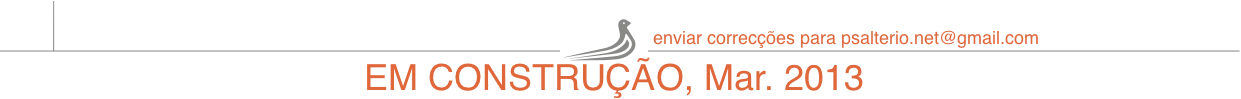
\includegraphics{_images/bkground_page_bottom.png}
}}








%
%Font Sizes
%
%\tiny
%\scriptsize
%\footnotesize
%\small
%\normalsize
%\large
%\Large
%\LARGE
%\huge
%\Huge


%\renewcommand{\thesongnum}{A\arabic{songnum}}
%\renewcommand{\printsongnum}[1]{\sffamily\bfseries\huge\MakeUppercase#1}
%\setlength{\songnumwidth}{2cm} % box width
%\renewcommand{\snumbgcolor}{white}

%change font for Title
%\renewcommand{\stitlefont}{\sffamily\bfseries\huge\MakeUppercase} %song title

%remove verse numbers
%\noversenumbers 
% make left separation
%\setlength{\versenumwidth}{2.0cm}

%verse separations
%\versesep=15pt
%\afterpreludeskip=2pt
%\beforepostludeskip=2pt
%\baselineadj=10pt

% separation between chords and lyrics
%\renewcommand{\clineparams}{ 
%\baselineskip=10pt 
%\lineskiplimit=2pt 
%\lineskip=5pt
%}

% change font for lyrics
%\renewcommand{\lyricfont}{\sffamily}
%\renewcommand{\lyricfont}{\sffamily\small}
%\renewcommand{\lyricfont}{\sffamily\large}
%\renewcommand{\chorusfont}{\sffamily}
%\renewcommand{\chorusfont}{\sffamily\large}

%change the Chords formatting
\renewcommand{\printchord}[1]{\sffamily\color{blue}\it\normalsize#1}

%check http://www.tug.org/pracjourn/2006-1/schmidt/schmidt.pdf


%\renewcommand{\songauthors}[1]{tete #1}


%\renewcommand{\extendpostlude}
%{ \songcopyright\ \songlicense\unskip \ Used with permission.}

\setlength{\cbarwidth}{0pt}
%\setlength{\sbarheight}{0pt}

% music anf lyrics by
\newcommand{\musicLyricsBy}{} 
\newsongkey{mlby}{\def\musicLyricsBy{}}
                 {\def\musicLyricsBy{\sffamily\it\small letra e música por #1\par}}

% music anf lyrics by
\newcommand{\musicby}{} 
\newsongkey{music}{\def\musicby{}}
                 {\def\musicby{\sffamily\it\small música: #1\par}}

% music anf lyrics by
\newcommand{\lyricsby}{} 
\newsongkey{lyrics}{\def\lyricsby{}}
                 {\def\lyricsby{\sffamily\it\small letra: #1\par}}

%\renewcommand{\sharpsymbol}{\ensuremath{^\sharp}}
\renewcommand{\extendprelude}{
  \showrefs\showauthors 
  %{\bfseries\musicLyricsBy}
  {\bfseries\musicby}
  {\bfseries\lyricsby}
}

\def \gtabsOn{1}
\documentclass[10pt,a5paper,landscape]{article}

%packages
\usepackage[left=1cm,right=1cm,top=1cm,bottom=1cm]{geometry}

\usepackage[chorded]{\rootFolder/_include/psalterio} %must check the licence to change the name of the sty file!!!
%\usepackage[chorded]{resources/songs-old} %must check the licence to change the name of the sty file!!!

\usepackage[utf8]{inputenc}
%\usepackage[utf8,latin1]{inputenc}

\usepackage{graphicx}
\usepackage{wrapfig}
\usepackage{wallpaper}
\usepackage{color}
\usepackage{eso-pic} %for background pictures
\usepackage[bookmarks]{hyperref} 
%\usepackage{ifthen} %etoolbox is more up to date
\usepackage{etoolbox}

%\usepackage[xetex]{graphicx}
%\usepackage{fontspec,xunicode}
%\defaultfontfeatures{Mapping=tex-text,Scale=MatchLowercase}
%\setmainfont[Scale=.95]{Times}
%\setmonofont{Lucida Sans Typewriter}

%\usepackage[portuguese]{babel}
%\usepackage[latin1]{inputenc}
%\usepackage[utf8]{inputenc}
%\usepackage[T1]{fontenc}
%\usepackage[scaled]{uarial}
%\usepackage{helvet}
%\renewcommand{\familydefault}{\sfdefault}

%this removes the page number
\thispagestyle{empty}
\pagestyle{empty}
\songcolumns{2}

\parindent 0pt	


%add background picture
\newcommand\BackgroundPic{
\put(0,0){
\parbox[b][\paperheight]{\paperwidth}{%
\vfill
\centering

\includegraphics[width=\paperwidth,height=\paperheight,
keepaspectratio]{logo.png}%
\vfill
}}}

\newcommand\BottomPic{
\put(0,0){
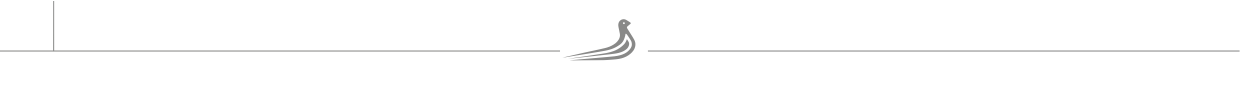
\includegraphics{\rootFolder/_images/bkground_page_bottom.png}
}}




%
%Font Sizes
%
%\tiny
%\scriptsize
%\footnotesize
%\small
%\normalsize
%\large
%\Large
%\LARGE
%\huge
%\Huge

%%% format song number
%\renewcommand{\thesongnum}{A\arabic{songnum}}
\renewcommand{\printsongnum}[1]{\sffamily\bfseries\huge\MakeUppercase#1}
\setlength{\songnumwidth}{1.5cm} % box width
%\renewcommand{\snumbgcolor}{white}

%%% format title
%change font for Title
%\renewcommand{\stitlefont}{\sffamily\bfseries\huge\MakeUppercase} 
\renewcommand{\stitlefont}{\sffamily\bfseries\huge}
%song title

%%% format verse numbers
%remove verse numbers
%\noversenumbers 
% make left separation
\setlength{\versenumwidth}{.5cm}


%verse separations
%\versesep=15pt
%\afterpreludeskip=2pt
%\beforepostludeskip=2pt
%\baselineadj=10pt

% separation between chords and lyrics
\renewcommand{\clineparams}{ 
\baselineskip=11pt 
%\lineskiplimit=2pt 
%\lineskip=5pt
}

%\setlength{\oddsidemargin}{0in}
%\setlength{\evensidemargin}{0in}

% change font for lyrics
%\renewcommand{\lyricfont}{\sffamily}
%\renewcommand{\lyricfont}{\sffamily\small}
\renewcommand{\lyricfont}{\sffamily\large}
%\renewcommand{\chorusfont}{\sffamily}
\renewcommand{\chorusfont}{\sffamily\large}

%change the Chords formatting
\renewcommand{\printchord}[1]{\sffamily\color{red}\it\normalsize#1}

%check http://www.tug.org/pracjourn/2006-1/schmidt/schmidt.pdf


%\renewcommand{\songauthors}[1]{tete #1}


%\renewcommand{\extendpostlude}
%{ \songcopyright\ \songlicense\unskip \ Used with permission.}

% chorus bar width
\setlength{\cbarwidth}{0pt}

%\renewcommand{\chorusjustify}{\justifyleft}


\setlength{\sbarheight}{0pt}

% music anf lyrics by
\newcommand{\musicLyricsBy}{} 
\newsongkey{mlby}{\def\musicLyricsBy{}}
                 {\def\musicLyricsBy{\sffamily\it\small letra e música por #1\par}}

% music by
\newcommand{\musicby}{} 
\newsongkey{musicby}{\def\musicby{}}
                 {\def\musicby{\sffamily\it\small música por #1\par}}

% lyrics by
\newcommand{\lyricsby}{} 
\newsongkey{lyricsby}{\def\lyricsby{}}
                 {\def\lyricsby{\sffamily\it\small letra por #1\par}}

% number
\newcommand{\psalterionumber}{} 
\newsongkey{psalterionumber}{\def\psalterionumber{}}
                 {\def\psalterionumber{\sffamily\it\small Psaltério #1\par}}


%\renewcommand{\sharpsymbol}{\ensuremath{^\sharp}}
\renewcommand{\extendprelude}{
  \showrefs\showauthors 
  {\bfseries\musicLyricsBy}
  {\bfseries\musicby}
  {\bfseries\lyricsby}
}

\def \gtabsOn{1}
%%\documentclass[10pt,a5paper,landscape]{article}
\documentclass[letterpaper]{article}

%packages
%\usepackage[left=1cm,right=1cm,top=1cm,bottom=1cm]{geometry}

%must check the licence to change the name of the sty file!!!
%\usepackage[chorded]{_include/psalterio} 
\usepackage[chorded]{_include/songs} 

%\usepackage[utf8]{inputenc}
\usepackage[utf8,latin1]{inputenc}

\usepackage{graphicx}
\usepackage{wrapfig}
\usepackage{wallpaper}
\usepackage{color}
\usepackage{eso-pic} %for background pictures
\usepackage[bookmarks]{hyperref} 
%\usepackage{ifthen} %etoolbox is more up to date
\usepackage{etoolbox}




\setlength{\oddsidemargin}{0in}
\setlength{\evensidemargin}{0in}
\setlength{\textwidth}{6.5in}
\setlength{\topmargin}{0in}
\setlength{\topskip}{0in}
\setlength{\headheight}{0in}
\setlength{\headsep}{0in}
\setlength{\textheight}{9.1in}
\settowidth{\versenumwidth}{1.\ }
\pagestyle{empty}

% for the index
\newindex{titleidx}{cbtitle}
%\newauthorindex{authidx}{cbauth}
%\newscripindex{scripidx}{cbscrip}



%\usepackage[xetex]{graphicx}
%\usepackage{fontspec,xunicode}
%\defaultfontfeatures{Mapping=tex-text,Scale=MatchLowercase}
%\setmainfont[Scale=.95]{Times}
%\setmonofont{Lucida Sans Typewriter}

%\usepackage[portuguese]{babel}
%\usepackage[latin1]{inputenc}
%\usepackage[utf8]{inputenc}
%\usepackage[T1]{fontenc}
%\usepackage[scaled]{uarial}
%\usepackage{helvet}
%\renewcommand{\familydefault}{\sfdefault}

%this removes the page number
%\thispagestyle{empty}
%\pagestyle{empty}
%\songcolumns{1}

%\parindent 0pt	


%add background picture
\newcommand\BackgroundPic{
\put(0,0){
\parbox[b][\paperheight]{\paperwidth}{%
\vfill
\centering

\includegraphics[width=\paperwidth,height=\paperheight,
keepaspectratio]{logo.png}%
\vfill
}}}

\newcommand\BottomPic{
\put(0,0){
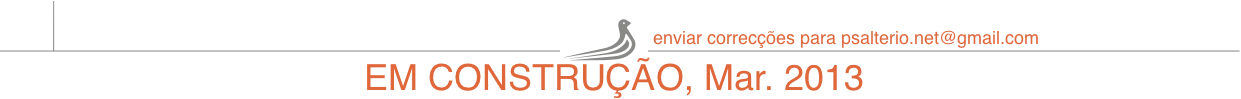
\includegraphics{_images/bkground_page_bottom.png}
}}








%
%Font Sizes
%
%\tiny
%\scriptsize
%\footnotesize
%\small
%\normalsize
%\large
%\Large
%\LARGE
%\huge
%\Huge


%\renewcommand{\thesongnum}{A\arabic{songnum}}
%\renewcommand{\printsongnum}[1]{\sffamily\bfseries\huge\MakeUppercase#1}
%\setlength{\songnumwidth}{2cm} % box width
%\renewcommand{\snumbgcolor}{white}

%change font for Title
%\renewcommand{\stitlefont}{\sffamily\bfseries\huge\MakeUppercase} %song title

%remove verse numbers
%\noversenumbers 
% make left separation
%\setlength{\versenumwidth}{2.0cm}

%verse separations
%\versesep=15pt
%\afterpreludeskip=2pt
%\beforepostludeskip=2pt
%\baselineadj=10pt

% separation between chords and lyrics
%\renewcommand{\clineparams}{ 
%\baselineskip=10pt 
%\lineskiplimit=2pt 
%\lineskip=5pt
%}

% change font for lyrics
%\renewcommand{\lyricfont}{\sffamily}
%\renewcommand{\lyricfont}{\sffamily\small}
%\renewcommand{\lyricfont}{\sffamily\large}
%\renewcommand{\chorusfont}{\sffamily}
%\renewcommand{\chorusfont}{\sffamily\large}

%change the Chords formatting
%\renewcommand{\printchord}[1]{\sffamily\color{red}\it\normalsize#1}

%check http://www.tug.org/pracjourn/2006-1/schmidt/schmidt.pdf


%\renewcommand{\songauthors}[1]{tete #1}


%\renewcommand{\extendpostlude}
%{ \songcopyright\ \songlicense\unskip \ Used with permission.}

%\setlength{\cbarwidth}{0pt}
%\setlength{\sbarheight}{0pt}

% music anf lyrics by
\newcommand{\musicLyricsBy}{} 
\newsongkey{mlby}{\def\musicLyricsBy{}}
                 {\def\musicLyricsBy{\sffamily\it\small letra e música por #1\par}}

% music anf lyrics by
\newcommand{\musicby}{} 
\newsongkey{music}{\def\musicby{}}
                 {\def\musicby{música: #1\par}}

% music anf lyrics by
\newcommand{\lyricsby}{} 
\newsongkey{lyrics}{\def\lyricsby{}}
                 {\def\lyricsby{letra: #1\par}}

%\renewcommand{\sharpsymbol}{\ensuremath{^\sharp}}
\renewcommand{\extendprelude}{
  \showrefs\showauthors 
  %{\bfseries\musicLyricsBy}
  {\bfseries\musicby}
  {\bfseries\lyricsby}
}

\def \gtabsOn{1}

% this includes all the guitar tabs that may be needed
% must complete all the chords used in psalterio

% Cb chords

% C chords
\def \gtabCb{\gtab{Cb}{X32010:X32010}}
\def \gtabC{\gtab{C}{X32010:032010}}
\def \gtabCm{\gtab{Cm}{3:113321:004320}}

\def \gtabCsharpSusFour{\gtab{C\#sus4}{4:XX3341:XX2341}}

% Db chords

% D chords
\def \gtabD{\gtab{D}{X00232:000132}}
\def \gtabDm{\gtab{Dm}{X00231:000231}}
\def \gtabDfour{\gtab{D4}{X00233:000134}}
\def \gtabDseven{\gtab{D7}{X00212:000213}}
\def \gtabDsevenPlus{\gtab{D7+}{X00222:000111}}

% D#/Eb chords
\def \gtabDsharp{\gtab{D\#}{2:XX0232:000132}}

% E chords
\def \gtabE{\gtab{E}{022100:023100}}
\def \gtabEseven{\gtab{E}{020100:020100}}

\def \gtabEm{\gtab{Em}{022000:012000}}
\def \gtabEmSeven{\gtab{Em7}{022030:012040}}

% Gb chords

% F chords
\def \gtabF{\gtab{F}{1:133211:034200}}
\def \gtabFm{\gtab{Fm}{1:133111:034000}}


% F# chords
\def \gtabFsharpMinor{\gtab{F\#m}{2:133111:034000}}
\def \gtabFsharpMinorSeven{\gtab{F\#m7}{2:131131:030040}}

% Gb chords

% G chords
\def \gtabG{\gtab{G}{320033:210034}}
\def \gtabGseven{\gtab{G7}{320001:320001}}
\def \gtabGfret{\gtab{(G)}{3:133211:034200}}
\def \gtabGm{\gtab{Gm}{3:133111:034000}}


% G# / Ab chords

% A chords
\def \gtabA{\gtab{A}{X02220:001230}}
\def \gtabAm{\gtab{Am}{X02210:002310}}
\def \gtabAmSeven{\gtab{Am7}{X02010:002010}}
\def \gtabAfour{\gtab{A4}{X02230:001230}}
\def \gtabAseven{\gtab{A7}{X02020:001030}}

% Bb chords
\def \gtabBb{\gtab{Bb}{X13331}}

% B chords
\def \gtabB{\gtab{B}{X13331:003210}}
\def \gtabBm{\gtab{Bm}{X13321:003420}}
\def \gtabBmSeven{\gtab{Bm7}{X13121:003020}}



% after any { or } at the end of a line inside the macro definition add %, otherwise you'll get an extra space
\newcommand{\guitarTab}[1]{%
\ifstrequal{#1}{Cb}      {\gtab{Cb}{X32010:X32010}      }{}%
\ifstrequal{#1}{C}        { \gtab{C}{X32010:032010}       }{}%
%
%G
%
\ifstrequal{#1}{G}       { \gtab{G}{320033:210034}       }{}%
\ifstrequal{#1}{G7}     { \gtab{G7}{320001:320001}     }{}%
\ifstrequal{#1}{Gfret}  { \gtab{G}{3:133211:034200}    }{}%
\ifstrequal{#1}{Gm}    { \gtab{Gm}{3:133111:034000}  }{}%
} %end \newcommand{\gtab}


\providebool{gchords}
\setbool{gchords}{false}

% set guitar chords vertical space separation with lyrics
%\def \gchordsVspace{5 mm}

\begin{document}

	%\showindex{Complete Index of Songs}{titleidx}
	%\showindex{Index of Authors and Composers}{authidx}
	%\showindex{Index of Scripture}{scripidx}

	%\songsection{Psalterio} % with title
	\songsection{} % no title

	\AddToShipoutPicture{\BottomPic}
	
	\begin{songs}{}
	%\begin{songs}{titleidx,authidx,scripidx}
	%\begin{songs}{titleidx}
	
	%%%%%%%%%%%%%%%%%%%%%%%%%%%%%%%%%%%%%%%%%%%%%%%%%%%%%%%%%%%%%%%%%%%%%%%%%%%%
% include packages and formatting for the document
%%%%%%%%%%%%%%%%%%%%%%%%%%%%%%%%%%%%%%%%%%%%%%%%%%%%%%%%%%%%%%%%%%%%%%%%%%%
%\def \includeFolder{../_include}

% this has all the necessary packages and formatting for the document
\documentclass[10pt,a5paper]{article}

%define include folder
\def \includeFolder{_include}

%packages
\usepackage[left=1cm,right=1cm,top=1cm,bottom=1cm]{geometry}

\usepackage[chorded]{\includeFolder/psalterio} %must check the licence to change the name of the sty file!!!
%\usepackage[chorded]{resources/songs-old} %must check the licence to change the name of the sty file!!!

\usepackage[utf8]{inputenc}

\usepackage{graphicx}
\usepackage{wrapfig}
\usepackage{wallpaper}
\usepackage{color}
\usepackage{eso-pic} %for background pictures
\usepackage[bookmarks]{hyperref} 
%\usepackage{ifthen} %etoolbox is more up to date
\usepackage{etoolbox}


%\usepackage[xetex]{graphicx}
%\usepackage{fontspec,xunicode}
%\defaultfontfeatures{Mapping=tex-text,Scale=MatchLowercase}
%\setmainfont[Scale=.95]{Times}
%\setmonofont{Lucida Sans Typewriter}

%\usepackage[portuguese]{babel}
%\usepackage[latin1]{inputenc}
%\usepackage[utf8]{inputenc}
%\usepackage[T1]{fontenc}
%\usepackage[scaled]{uarial}
%\usepackage{helvet}
%\renewcommand{\familydefault}{\sfdefault}

%this removes the page number
\thispagestyle{empty}
\pagestyle{empty}
\songcolumns{1}

\parindent 0pt

%add background picture
\newcommand\BackgroundPic{
\put(0,0){
\parbox[b][\paperheight]{\paperwidth}{%
\vfill
\centering

\includegraphics[width=\paperwidth,height=\paperheight,
keepaspectratio]{logo.png}%
\vfill
}}}

\newcommand\BottomPic{
\put(0,0){
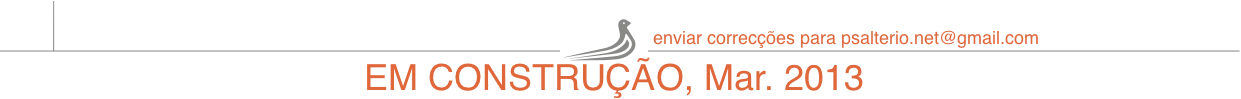
\includegraphics{_images/bkground_page_bottom.png}
}}





% this includes all the guitar tabs that may be needed
% must complete all the chords used in psalterio

% Cb chords

% C chords
\def \gtabCb{\gtab{Cb}{X32010:X32010}}
\def \gtabC{\gtab{C}{X32010:032010}}
\def \gtabCm{\gtab{Cm}{3:113321:004320}}

\def \gtabCsharpSusFour{\gtab{C\#sus4}{4:XX3341:XX2341}}

% Db chords

% D chords
\def \gtabD{\gtab{D}{X00232:000132}}
\def \gtabDm{\gtab{Dm}{X00231:000231}}
\def \gtabDfour{\gtab{D4}{X00233:000134}}
\def \gtabDseven{\gtab{D7}{X00212:000213}}
\def \gtabDsevenPlus{\gtab{D7+}{X00222:000111}}

% D#/Eb chords
\def \gtabDsharp{\gtab{D\#}{2:XX0232:000132}}

% E chords
\def \gtabE{\gtab{E}{022100:023100}}
\def \gtabEseven{\gtab{E}{020100:020100}}

\def \gtabEm{\gtab{Em}{022000:012000}}
\def \gtabEmSeven{\gtab{Em7}{022030:012040}}

% Gb chords

% F chords
\def \gtabF{\gtab{F}{1:133211:034200}}
\def \gtabFm{\gtab{Fm}{1:133111:034000}}


% F# chords
\def \gtabFsharpMinor{\gtab{F\#m}{2:133111:034000}}
\def \gtabFsharpMinorSeven{\gtab{F\#m7}{2:131131:030040}}

% Gb chords

% G chords
\def \gtabG{\gtab{G}{320033:210034}}
\def \gtabGseven{\gtab{G7}{320001:320001}}
\def \gtabGfret{\gtab{(G)}{3:133211:034200}}
\def \gtabGm{\gtab{Gm}{3:133111:034000}}


% G# / Ab chords

% A chords
\def \gtabA{\gtab{A}{X02220:001230}}
\def \gtabAm{\gtab{Am}{X02210:002310}}
\def \gtabAmSeven{\gtab{Am7}{X02010:002010}}
\def \gtabAfour{\gtab{A4}{X02230:001230}}
\def \gtabAseven{\gtab{A7}{X02020:001030}}

% Bb chords
\def \gtabBb{\gtab{Bb}{X13331}}

% B chords
\def \gtabB{\gtab{B}{X13331:003210}}
\def \gtabBm{\gtab{Bm}{X13321:003420}}
\def \gtabBmSeven{\gtab{Bm7}{X13121:003020}}



% after any { or } at the end of a line inside the macro definition add %, otherwise you'll get an extra space
\newcommand{\guitarTab}[1]{%
\ifstrequal{#1}{Cb}      {\gtab{Cb}{X32010:X32010}      }{}%
\ifstrequal{#1}{C}        { \gtab{C}{X32010:032010}       }{}%
%
%G
%
\ifstrequal{#1}{G}       { \gtab{G}{320033:210034}       }{}%
\ifstrequal{#1}{G7}     { \gtab{G7}{320001:320001}     }{}%
\ifstrequal{#1}{Gfret}  { \gtab{G}{3:133211:034200}    }{}%
\ifstrequal{#1}{Gm}    { \gtab{Gm}{3:133111:034000}  }{}%
} %end \newcommand{\gtab}

%muda aqui o numero da musica em que estas a trabalhar
%\def \selectSong{114}

\providebool{gchords}
\setbool{gchords}{true}

% set guitar chords vertical space separation with lyrics
\def \gchordsVspace{5 mm}

\begin{document}
	
	
	\AddToShipoutPicture*{\BottomPic}
	
	\begin{songs}{}
	
	%format file
	%
%Font Sizes
%
%\tiny
%\scriptsize
%\footnotesize
%\small
%\normalsize
%\large
%\Large
%\LARGE
%\huge
%\Huge


%\renewcommand{\thesongnum}{A\arabic{songnum}}
\renewcommand{\printsongnum}[1]{\sffamily\bfseries\huge\MakeUppercase#1}
\setlength{\songnumwidth}{2cm} % box width
%\renewcommand{\snumbgcolor}{white}

%change font for Title
\renewcommand{\stitlefont}{\sffamily\bfseries\huge\MakeUppercase} %song title

%remove verse numbers
%\noversenumbers 
% make left separation
\setlength{\versenumwidth}{2.0cm}

%verse separations
%\versesep=15pt
%\afterpreludeskip=2pt
%\beforepostludeskip=2pt
%\baselineadj=10pt

% separation between chords and lyrics
\renewcommand{\clineparams}{ 
\baselineskip=10pt 
%\lineskiplimit=2pt 
%\lineskip=5pt
}

% change font for lyrics
%\renewcommand{\lyricfont}{\sffamily}
%\renewcommand{\lyricfont}{\sffamily\small}
\renewcommand{\lyricfont}{\sffamily\large}
%\renewcommand{\chorusfont}{\sffamily}
\renewcommand{\chorusfont}{\sffamily\large}

%change the Chords formatting
\renewcommand{\printchord}[1]{\sffamily\color{red}\it\normalsize#1}

%check http://www.tug.org/pracjourn/2006-1/schmidt/schmidt.pdf


%\renewcommand{\songauthors}[1]{tete #1}


%\renewcommand{\extendpostlude}
%{ \songcopyright\ \songlicense\unskip \ Used with permission.}

\setlength{\cbarwidth}{0pt}
\setlength{\sbarheight}{0pt}

% music anf lyrics by
\newcommand{\musicLyricsBy}{} 
\newsongkey{mlby}{\def\musicLyricsBy{}}
                 {\def\musicLyricsBy{\sffamily\it\small letra e música por #1\par}}

% music anf lyrics by
\newcommand{\musicby}{} 
\newsongkey{music}{\def\musicby{}}
                 {\def\musicby{\sffamily\it\small música: #1\par}}

% music anf lyrics by
\newcommand{\lyricsby}{} 
\newsongkey{lyrics}{\def\lyricsby{}}
                 {\def\lyricsby{\sffamily\it\small letra: #1\par}}

%\renewcommand{\sharpsymbol}{\ensuremath{^\sharp}}
\renewcommand{\extendprelude}{
  \showrefs\showauthors 
  %{\bfseries\musicLyricsBy}
  {\bfseries\musicby}
  {\bfseries\lyricsby}
}

\def \gtabsOn{1}
	

%%%%%%%%%%%%%%%%%%%%%%%%%%%%%%%%%%%%%%%%%%%%%%%%%%%%%%%%%%%%%%%%%%%%%%%%%%%
% set song number
%%%%%%%%%%%%%%%%%%%%%%%%%%%%%%%%%%%%%%%%%%%%%%%%%%%%%%%%%%%%%%%%%%%%%%%%%%%
\setcounter{songnum}{0}

%%%%%%%%%%%%%%%%%%%%%%%%%%%%%%%%%%%%%%%%%%%%%%%%%%%%%%%%%%%%%%%%%%%%%%%%%%%
% begin song latex formating, set the title and other info
%%%%%%%%%%%%%%%%%%%%%%%%%%%%%%%%%%%%%%%%%%%%%%%%%%%%%%%%%%%%%%%%%%%%%%%%%%%
\beginsong{Template}[            % song title ...
% music and lyric by
musiclyricsby={Arnaldo Ferreira},     
% music and lyric by
musicby={Joana Lantrinha},    
% music and lyric by
lyricsby={Joana Lantrinha},    
% bible verse                      
bible_verse={Revelation 5:13},%sr
% licence
credits={Public domain.},%cr
% arrangement by
%arrangementby={my},
% index title ...	
index={Template}]              

%%%%%%%%%%%%%%%%%%%%%%%%%%%%%%%%%%%%%%%%%%%%%%%%%%%%%%%%%%%%%%%%%%%%%%%%%%%
% verse #1
%%%%%%%%%%%%%%%%%%%%%%%%%%%%%%%%%%%%%%%%%%%%%%%%%%%%%%%%%%%%%%%%%%%%%%%%%%%
\beginverse                       % start verse
\[D]Lá es\[G]tá o meu tes\[D A]ouro,
\chordsoff                        % turn off chords
Lá onde não há choro.
\chordson                         % turn on chords
Onde \[F#m Bm]{todos cantaremos} \[F#m Bm]juntos
\[G]Hinos de lou\[A]vor... ao Se\[D]nhor\[G D A].
\endverse                         % end verse

%%%%%%%%%%%%%%%%%%%%%%%%%%%%%%%%%%%%%%%%%%%%%%%%%%%%%%%%%%%%%%%%%%%%%%%%%%%
% chorus
%%%%%%%%%%%%%%%%%%%%%%%%%%%%%%%%%%%%%%%%%%%%%%%%%%%%%%%%%%%%%%%%%%%%%%%%%%%
\beginchorus                      % start chorus
\[F#m Bm]Aleluia, \[F#m Bm]Aleluia
\[G]Hinos de lou\[A]vor... ao Se\[D]nhor\[G D A]. 
(canon com a estrofe)
\endchorus                        % end chorus

%%%%%%%%%%%%%%%%%%%%%%%%%%%%%%%%%%%%%%%%%%%%%%%%%%%%%%%%%%%%%%%%%%%%%%%%%%%
% verse #2
%%%%%%%%%%%%%%%%%%%%%%%%%%%%%%%%%%%%%%%%%%%%%%%%%%%%%%%%%%%%%%%%%%%%%%%%%%%
\beginverse                       % start verse
\chordsoff                        % chords formating off
Exemplo.
Exemplo.
Exemplo.
\chordson
\endverse                         % start verse

%%%%%%%%%%%%%%%%%%%%%%%%%%%%%%%%%%%%%%%%%%%%%%%%%%%%%%%%%%%%%%%%%%%%%%%%%%%
% print guitar tabs used in this song
%%%%%%%%%%%%%%%%%%%%%%%%%%%%%%%%%%%%%%%%%%%%%%%%%%%%%%%%%%%%%%%%%%%%%%%%%%%
\ifbool{gchords}{                 % if the guitar chords are to be printed
\vspace{\gchordsVspace}           % set a vertical space of 10 pt 

\gtabD
\gtabG
\gtabA
\gtabFsharpMinor
\gtabBm

}                                 % end if

%%%%%%%%%%%%%%%%%%%%%%%%%%%%%%%%%%%%%%%%%%%%%%%%%%%%%%%%%%%%%%%%%%%%%%%%%%%
% end song latex formating
%%%%%%%%%%%%%%%%%%%%%%%%%%%%%%%%%%%%%%%%%%%%%%%%%%%%%%%%%%%%%%%%%%%%%%%%%%%
\endsong                          % end song
%	 %lilypond-book --output=out --pdf  106single.tex
	 %\lilypondfile[]{E_101.ly}
	
\end{document}
	% numero 1 antigo agora passou ao 4, hino dos companheiros
	% o hino primeiro sera o do psalterio?
	% percentagem é comentário
% 1 - \setcounter{songnum}{0} - numero da musica
% 2 - \beginsong{Hino Ticoes}[ - título da música
% 3 -  index={Hino Ticoes}] - entrada do indice da musica
% 4 - \beginverse , depois desta linha adicionar a letra
%%%%%%%%%%%%%%%%%%%%%%%%%%%%%%%%%%%%%%%%%%%%%%%%%%%%%%%%%%%%%%%%%%%%%%%%%%%
% this has all the necessary packages and formatting for the document
%%%%%%%%%%%%%%%%%%%%%%%%%%%%%%%%%%%%%%%%%%%%%%%%%%%%%%%%%%%%%%%%%%%%%%%%%%%
%\def \includeFolder{../_include}

% this has all the necessary packages and formatting for the document
\documentclass[10pt,a5paper]{article}

%define include folder
\def \includeFolder{_include}

%packages
\usepackage[left=1cm,right=1cm,top=1cm,bottom=1cm]{geometry}

\usepackage[chorded]{\includeFolder/psalterio} %must check the licence to change the name of the sty file!!!
%\usepackage[chorded]{resources/songs-old} %must check the licence to change the name of the sty file!!!

\usepackage[utf8]{inputenc}

\usepackage{graphicx}
\usepackage{wrapfig}
\usepackage{wallpaper}
\usepackage{color}
\usepackage{eso-pic} %for background pictures
\usepackage[bookmarks]{hyperref} 
%\usepackage{ifthen} %etoolbox is more up to date
\usepackage{etoolbox}


%\usepackage[xetex]{graphicx}
%\usepackage{fontspec,xunicode}
%\defaultfontfeatures{Mapping=tex-text,Scale=MatchLowercase}
%\setmainfont[Scale=.95]{Times}
%\setmonofont{Lucida Sans Typewriter}

%\usepackage[portuguese]{babel}
%\usepackage[latin1]{inputenc}
%\usepackage[utf8]{inputenc}
%\usepackage[T1]{fontenc}
%\usepackage[scaled]{uarial}
%\usepackage{helvet}
%\renewcommand{\familydefault}{\sfdefault}

%this removes the page number
\thispagestyle{empty}
\pagestyle{empty}
\songcolumns{1}

\parindent 0pt

%add background picture
\newcommand\BackgroundPic{
\put(0,0){
\parbox[b][\paperheight]{\paperwidth}{%
\vfill
\centering

\includegraphics[width=\paperwidth,height=\paperheight,
keepaspectratio]{logo.png}%
\vfill
}}}

\newcommand\BottomPic{
\put(0,0){
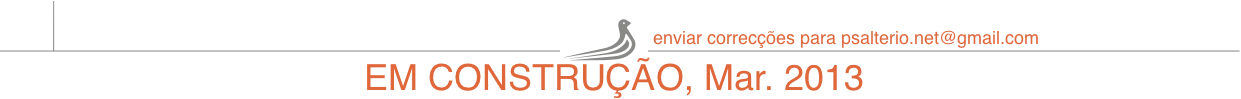
\includegraphics{_images/bkground_page_bottom.png}
}}





% this includes all the guitar tabs that may be needed
% must complete all the chords used in psalterio

% Cb chords

% C chords
\def \gtabCb{\gtab{Cb}{X32010:X32010}}
\def \gtabC{\gtab{C}{X32010:032010}}
\def \gtabCm{\gtab{Cm}{3:113321:004320}}

\def \gtabCsharpSusFour{\gtab{C\#sus4}{4:XX3341:XX2341}}

% Db chords

% D chords
\def \gtabD{\gtab{D}{X00232:000132}}
\def \gtabDm{\gtab{Dm}{X00231:000231}}
\def \gtabDfour{\gtab{D4}{X00233:000134}}
\def \gtabDseven{\gtab{D7}{X00212:000213}}
\def \gtabDsevenPlus{\gtab{D7+}{X00222:000111}}

% D#/Eb chords
\def \gtabDsharp{\gtab{D\#}{2:XX0232:000132}}

% E chords
\def \gtabE{\gtab{E}{022100:023100}}
\def \gtabEseven{\gtab{E}{020100:020100}}

\def \gtabEm{\gtab{Em}{022000:012000}}
\def \gtabEmSeven{\gtab{Em7}{022030:012040}}

% Gb chords

% F chords
\def \gtabF{\gtab{F}{1:133211:034200}}
\def \gtabFm{\gtab{Fm}{1:133111:034000}}


% F# chords
\def \gtabFsharpMinor{\gtab{F\#m}{2:133111:034000}}
\def \gtabFsharpMinorSeven{\gtab{F\#m7}{2:131131:030040}}

% Gb chords

% G chords
\def \gtabG{\gtab{G}{320033:210034}}
\def \gtabGseven{\gtab{G7}{320001:320001}}
\def \gtabGfret{\gtab{(G)}{3:133211:034200}}
\def \gtabGm{\gtab{Gm}{3:133111:034000}}


% G# / Ab chords

% A chords
\def \gtabA{\gtab{A}{X02220:001230}}
\def \gtabAm{\gtab{Am}{X02210:002310}}
\def \gtabAmSeven{\gtab{Am7}{X02010:002010}}
\def \gtabAfour{\gtab{A4}{X02230:001230}}
\def \gtabAseven{\gtab{A7}{X02020:001030}}

% Bb chords
\def \gtabBb{\gtab{Bb}{X13331}}

% B chords
\def \gtabB{\gtab{B}{X13331:003210}}
\def \gtabBm{\gtab{Bm}{X13321:003420}}
\def \gtabBmSeven{\gtab{Bm7}{X13121:003020}}



% after any { or } at the end of a line inside the macro definition add %, otherwise you'll get an extra space
\newcommand{\guitarTab}[1]{%
\ifstrequal{#1}{Cb}      {\gtab{Cb}{X32010:X32010}      }{}%
\ifstrequal{#1}{C}        { \gtab{C}{X32010:032010}       }{}%
%
%G
%
\ifstrequal{#1}{G}       { \gtab{G}{320033:210034}       }{}%
\ifstrequal{#1}{G7}     { \gtab{G7}{320001:320001}     }{}%
\ifstrequal{#1}{Gfret}  { \gtab{G}{3:133211:034200}    }{}%
\ifstrequal{#1}{Gm}    { \gtab{Gm}{3:133111:034000}  }{}%
} %end \newcommand{\gtab}

%muda aqui o numero da musica em que estas a trabalhar
%\def \selectSong{114}

\providebool{gchords}
\setbool{gchords}{true}

% set guitar chords vertical space separation with lyrics
\def \gchordsVspace{5 mm}

\begin{document}
	
	
	\AddToShipoutPicture*{\BottomPic}
	
	\begin{songs}{}
	
	%format file
	%
%Font Sizes
%
%\tiny
%\scriptsize
%\footnotesize
%\small
%\normalsize
%\large
%\Large
%\LARGE
%\huge
%\Huge


%\renewcommand{\thesongnum}{A\arabic{songnum}}
\renewcommand{\printsongnum}[1]{\sffamily\bfseries\huge\MakeUppercase#1}
\setlength{\songnumwidth}{2cm} % box width
%\renewcommand{\snumbgcolor}{white}

%change font for Title
\renewcommand{\stitlefont}{\sffamily\bfseries\huge\MakeUppercase} %song title

%remove verse numbers
%\noversenumbers 
% make left separation
\setlength{\versenumwidth}{2.0cm}

%verse separations
%\versesep=15pt
%\afterpreludeskip=2pt
%\beforepostludeskip=2pt
%\baselineadj=10pt

% separation between chords and lyrics
\renewcommand{\clineparams}{ 
\baselineskip=10pt 
%\lineskiplimit=2pt 
%\lineskip=5pt
}

% change font for lyrics
%\renewcommand{\lyricfont}{\sffamily}
%\renewcommand{\lyricfont}{\sffamily\small}
\renewcommand{\lyricfont}{\sffamily\large}
%\renewcommand{\chorusfont}{\sffamily}
\renewcommand{\chorusfont}{\sffamily\large}

%change the Chords formatting
\renewcommand{\printchord}[1]{\sffamily\color{red}\it\normalsize#1}

%check http://www.tug.org/pracjourn/2006-1/schmidt/schmidt.pdf


%\renewcommand{\songauthors}[1]{tete #1}


%\renewcommand{\extendpostlude}
%{ \songcopyright\ \songlicense\unskip \ Used with permission.}

\setlength{\cbarwidth}{0pt}
\setlength{\sbarheight}{0pt}

% music anf lyrics by
\newcommand{\musicLyricsBy}{} 
\newsongkey{mlby}{\def\musicLyricsBy{}}
                 {\def\musicLyricsBy{\sffamily\it\small letra e música por #1\par}}

% music anf lyrics by
\newcommand{\musicby}{} 
\newsongkey{music}{\def\musicby{}}
                 {\def\musicby{\sffamily\it\small música: #1\par}}

% music anf lyrics by
\newcommand{\lyricsby}{} 
\newsongkey{lyrics}{\def\lyricsby{}}
                 {\def\lyricsby{\sffamily\it\small letra: #1\par}}

%\renewcommand{\sharpsymbol}{\ensuremath{^\sharp}}
\renewcommand{\extendprelude}{
  \showrefs\showauthors 
  %{\bfseries\musicLyricsBy}
  {\bfseries\musicby}
  {\bfseries\lyricsby}
}

\def \gtabsOn{1}
	
%%%%%%%%%%%%%%%%%%%%%%%%%%%%%%%%%%%%%%%%%%%%%%%%%%%%%%%%%%%%%%%%%%%%%%%%%%%
% set song number
%%%%%%%%%%%%%%%%%%%%%%%%%%%%%%%%%%%%%%%%%%%%%%%%%%%%%%%%%%%%%%%%%%%%%%%%%%%
\setcounter{songnum}{2}       % song number
%%%%%%%%%%%%%%%%%%%%%%%%%%%%%%%%%%%%%%%%%%%%%%%%%%%%%%%%%%%%%%%%%%%%%%%%%%%
% begin song latex formating, set the title and other info
%%%%%%%%%%%%%%%%%%%%%%%%%%%%%%%%%%%%%%%%%%%%%%%%%%%%%%%%%%%%%%%%%%%%%%%%%%%
\beginsong{Hino dos Tições}[            % song title ...
    %mlby={},                           % music and lyric by
    %sr={Revelation 5:13},        % bible verse
    %cr={Public domain.},         % licence
    %arr={my},                          % arrangement by
    index={Hino dos Tições}]               % index title ...	
%%%%%%%%%%%%%%%%%%%%%%%%%%%%%%%%%%%%%%%%%%%%%%%%%%%%%%%%%%%%%%%%%%%%%%%%%%%
% verse #1
%%%%%%%%%%%%%%%%%%%%%%%%%%%%%%%%%%%%%%%%%%%%%%%%%%%%%%%%%%%%%%%%%%%%%%%%%%%
\beginverse
\[C]Á fogueira levemos o noss\[G7]o tição
E ou\[C]çamos cantar sua fe\[G7]liz can\[C]ção.
Sobe \[Dm]chama lig\[C]eira, fogo \[G7]bom tão quente e \[C]bom.
No me\[Dm]io des\[Am]ta cla\[C]reira, sobe, p\[G7]ois, sim, sobe \[C]mais,
Sobe e s\[Am]obe e \[F]sobe \[C]mais,
\[F]Fo\[Fm]go b\[C]om, tão qu\[F]ente \[G7]e \[C]bom.
\endverse
%%%%%%%%%%%%%%%%%%%%%%%%%%%%%%%%%%%%%%%%%%%%%%%%%%%%%%%%%%%%%%%%%%%%%%%%%%%
% verse #2
%%%%%%%%%%%%%%%%%%%%%%%%%%%%%%%%%%%%%%%%%%%%%%%%%%%%%%%%%%%%%%%%%%%%%%%%%%%
\beginverse
\[C]Ó Jesus, vem acende em nós\[G7] o Tição.
De um a\[C]mor puro e quente pelo\[G7] nosso ir\[C]mão.
De a\[Dm]mor nos in\[C]flama, ó Je\[G7]sus, sim, ó Je\[C]sus.
E que \[Dm]nós se\[Am]jamos \[C]chama dando \[G7]luz, inda ma\[C]is luz,
Dando \[Am]luz, in\[F]da mais \[C]luz,
\[F]Dan\[Fm]do a\[C]mor, lu\[F]z e \[G7]ca\[C]lor.
\endverse
%%%%%%%%%%%%%%%%%%%%%%%%%%%%%%%%%%%%%%%%%%%%%%%%%%%%%%%%%%%%%%%%%%%%%%%%%%%
% print guitar tabs used in this song
%%%%%%%%%%%%%%%%%%%%%%%%%%%%%%%%%%%%%%%%%%%%%%%%%%%%%%%%%%%%%%%%%%%%%%%%%%%
\ifbool{gchords}{                 % if the guitar chords are to be printed
\vspace{\gchordsVspace}           % set a vertical space of 10 pt 
\gtabC
\gtabF
%\gtabGseven
\gtabFsharpMinor
\gtabBm
}                                 % end if
%%%%%%%%%%%%%%%%%%%%%%%%%%%%%%%%%%%%%%%%%%%%%%%%%%%%%%%%%%%%%%%%%%%%%%%%%%%
% end song latex formating
%%%%%%%%%%%%%%%%%%%%%%%%%%%%%%%%%%%%%%%%%%%%%%%%%%%%%%%%%%%%%%%%%%%%%%%%%%%
\endsong                          % end song
%	 %lilypond-book --output=out --pdf  106single.tex
	 %\lilypondfile[]{E_101.ly}
	
\end{document}
	% percentagem é comentário
% 1 - \setcounter{songnum}{0} - numero da musica
% 2 - \beginsong{Hino Desbravadores}[ - tÌtulo da m˙sica
% 3 -  index={Hino Desbravadores}] - entrada do indice da musica
% 4 - \beginverse , depois desta linha adicionar a letra
%%%%%%%%%%%%%%%%%%%%%%%%%%%%%%%%%%%%%%%%%%%%%%%%%%%%%%%%%%%%%%%%%%%%%%%%%%%
% this has all the necessary packages and formatting for the document
%%%%%%%%%%%%%%%%%%%%%%%%%%%%%%%%%%%%%%%%%%%%%%%%%%%%%%%%%%%%%%%%%%%%%%%%%%%
%\def \includeFolder{../_include}

% this has all the necessary packages and formatting for the document
\documentclass[10pt,a5paper]{article}

%define include folder
\def \includeFolder{_include}

%packages
\usepackage[left=1cm,right=1cm,top=1cm,bottom=1cm]{geometry}

\usepackage[chorded]{\includeFolder/psalterio} %must check the licence to change the name of the sty file!!!
%\usepackage[chorded]{resources/songs-old} %must check the licence to change the name of the sty file!!!

\usepackage[utf8]{inputenc}

\usepackage{graphicx}
\usepackage{wrapfig}
\usepackage{wallpaper}
\usepackage{color}
\usepackage{eso-pic} %for background pictures
\usepackage[bookmarks]{hyperref} 
%\usepackage{ifthen} %etoolbox is more up to date
\usepackage{etoolbox}


%\usepackage[xetex]{graphicx}
%\usepackage{fontspec,xunicode}
%\defaultfontfeatures{Mapping=tex-text,Scale=MatchLowercase}
%\setmainfont[Scale=.95]{Times}
%\setmonofont{Lucida Sans Typewriter}

%\usepackage[portuguese]{babel}
%\usepackage[latin1]{inputenc}
%\usepackage[utf8]{inputenc}
%\usepackage[T1]{fontenc}
%\usepackage[scaled]{uarial}
%\usepackage{helvet}
%\renewcommand{\familydefault}{\sfdefault}

%this removes the page number
\thispagestyle{empty}
\pagestyle{empty}
\songcolumns{1}

\parindent 0pt

%add background picture
\newcommand\BackgroundPic{
\put(0,0){
\parbox[b][\paperheight]{\paperwidth}{%
\vfill
\centering

\includegraphics[width=\paperwidth,height=\paperheight,
keepaspectratio]{logo.png}%
\vfill
}}}

\newcommand\BottomPic{
\put(0,0){
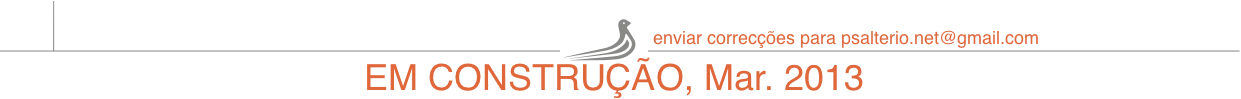
\includegraphics{_images/bkground_page_bottom.png}
}}





% this includes all the guitar tabs that may be needed
% must complete all the chords used in psalterio

% Cb chords

% C chords
\def \gtabCb{\gtab{Cb}{X32010:X32010}}
\def \gtabC{\gtab{C}{X32010:032010}}
\def \gtabCm{\gtab{Cm}{3:113321:004320}}

\def \gtabCsharpSusFour{\gtab{C\#sus4}{4:XX3341:XX2341}}

% Db chords

% D chords
\def \gtabD{\gtab{D}{X00232:000132}}
\def \gtabDm{\gtab{Dm}{X00231:000231}}
\def \gtabDfour{\gtab{D4}{X00233:000134}}
\def \gtabDseven{\gtab{D7}{X00212:000213}}
\def \gtabDsevenPlus{\gtab{D7+}{X00222:000111}}

% D#/Eb chords
\def \gtabDsharp{\gtab{D\#}{2:XX0232:000132}}

% E chords
\def \gtabE{\gtab{E}{022100:023100}}
\def \gtabEseven{\gtab{E}{020100:020100}}

\def \gtabEm{\gtab{Em}{022000:012000}}
\def \gtabEmSeven{\gtab{Em7}{022030:012040}}

% Gb chords

% F chords
\def \gtabF{\gtab{F}{1:133211:034200}}
\def \gtabFm{\gtab{Fm}{1:133111:034000}}


% F# chords
\def \gtabFsharpMinor{\gtab{F\#m}{2:133111:034000}}
\def \gtabFsharpMinorSeven{\gtab{F\#m7}{2:131131:030040}}

% Gb chords

% G chords
\def \gtabG{\gtab{G}{320033:210034}}
\def \gtabGseven{\gtab{G7}{320001:320001}}
\def \gtabGfret{\gtab{(G)}{3:133211:034200}}
\def \gtabGm{\gtab{Gm}{3:133111:034000}}


% G# / Ab chords

% A chords
\def \gtabA{\gtab{A}{X02220:001230}}
\def \gtabAm{\gtab{Am}{X02210:002310}}
\def \gtabAmSeven{\gtab{Am7}{X02010:002010}}
\def \gtabAfour{\gtab{A4}{X02230:001230}}
\def \gtabAseven{\gtab{A7}{X02020:001030}}

% Bb chords
\def \gtabBb{\gtab{Bb}{X13331}}

% B chords
\def \gtabB{\gtab{B}{X13331:003210}}
\def \gtabBm{\gtab{Bm}{X13321:003420}}
\def \gtabBmSeven{\gtab{Bm7}{X13121:003020}}



% after any { or } at the end of a line inside the macro definition add %, otherwise you'll get an extra space
\newcommand{\guitarTab}[1]{%
\ifstrequal{#1}{Cb}      {\gtab{Cb}{X32010:X32010}      }{}%
\ifstrequal{#1}{C}        { \gtab{C}{X32010:032010}       }{}%
%
%G
%
\ifstrequal{#1}{G}       { \gtab{G}{320033:210034}       }{}%
\ifstrequal{#1}{G7}     { \gtab{G7}{320001:320001}     }{}%
\ifstrequal{#1}{Gfret}  { \gtab{G}{3:133211:034200}    }{}%
\ifstrequal{#1}{Gm}    { \gtab{Gm}{3:133111:034000}  }{}%
} %end \newcommand{\gtab}

%muda aqui o numero da musica em que estas a trabalhar
%\def \selectSong{114}

\providebool{gchords}
\setbool{gchords}{true}

% set guitar chords vertical space separation with lyrics
\def \gchordsVspace{5 mm}

\begin{document}
	
	
	\AddToShipoutPicture*{\BottomPic}
	
	\begin{songs}{}
	
	%format file
	%
%Font Sizes
%
%\tiny
%\scriptsize
%\footnotesize
%\small
%\normalsize
%\large
%\Large
%\LARGE
%\huge
%\Huge


%\renewcommand{\thesongnum}{A\arabic{songnum}}
\renewcommand{\printsongnum}[1]{\sffamily\bfseries\huge\MakeUppercase#1}
\setlength{\songnumwidth}{2cm} % box width
%\renewcommand{\snumbgcolor}{white}

%change font for Title
\renewcommand{\stitlefont}{\sffamily\bfseries\huge\MakeUppercase} %song title

%remove verse numbers
%\noversenumbers 
% make left separation
\setlength{\versenumwidth}{2.0cm}

%verse separations
%\versesep=15pt
%\afterpreludeskip=2pt
%\beforepostludeskip=2pt
%\baselineadj=10pt

% separation between chords and lyrics
\renewcommand{\clineparams}{ 
\baselineskip=10pt 
%\lineskiplimit=2pt 
%\lineskip=5pt
}

% change font for lyrics
%\renewcommand{\lyricfont}{\sffamily}
%\renewcommand{\lyricfont}{\sffamily\small}
\renewcommand{\lyricfont}{\sffamily\large}
%\renewcommand{\chorusfont}{\sffamily}
\renewcommand{\chorusfont}{\sffamily\large}

%change the Chords formatting
\renewcommand{\printchord}[1]{\sffamily\color{red}\it\normalsize#1}

%check http://www.tug.org/pracjourn/2006-1/schmidt/schmidt.pdf


%\renewcommand{\songauthors}[1]{tete #1}


%\renewcommand{\extendpostlude}
%{ \songcopyright\ \songlicense\unskip \ Used with permission.}

\setlength{\cbarwidth}{0pt}
\setlength{\sbarheight}{0pt}

% music anf lyrics by
\newcommand{\musicLyricsBy}{} 
\newsongkey{mlby}{\def\musicLyricsBy{}}
                 {\def\musicLyricsBy{\sffamily\it\small letra e música por #1\par}}

% music anf lyrics by
\newcommand{\musicby}{} 
\newsongkey{music}{\def\musicby{}}
                 {\def\musicby{\sffamily\it\small música: #1\par}}

% music anf lyrics by
\newcommand{\lyricsby}{} 
\newsongkey{lyrics}{\def\lyricsby{}}
                 {\def\lyricsby{\sffamily\it\small letra: #1\par}}

%\renewcommand{\sharpsymbol}{\ensuremath{^\sharp}}
\renewcommand{\extendprelude}{
  \showrefs\showauthors 
  %{\bfseries\musicLyricsBy}
  {\bfseries\musicby}
  {\bfseries\lyricsby}
}

\def \gtabsOn{1}
	
%%%%%%%%%%%%%%%%%%%%%%%%%%%%%%%%%%%%%%%%%%%%%%%%%%%%%%%%%%%%%%%%%%%%%%%%%%%
% set song number
%%%%%%%%%%%%%%%%%%%%%%%%%%%%%%%%%%%%%%%%%%%%%%%%%%%%%%%%%%%%%%%%%%%%%%%%%%%
\setcounter{songnum}{3}       % song number
%%%%%%%%%%%%%%%%%%%%%%%%%%%%%%%%%%%%%%%%%%%%%%%%%%%%%%%%%%%%%%%%%%%%%%%%%%%
% begin song latex formating, set the title and other info
%%%%%%%%%%%%%%%%%%%%%%%%%%%%%%%%%%%%%%%%%%%%%%%%%%%%%%%%%%%%%%%%%%%%%%%%%%%
\beginsong{Hino dos Desbravadores}[            % song title ...
    %mlby={},                           % music and lyric by
    %sr={Revelation 5:13},        % bible verse
    %cr={Public domain.},         % licence
    %arr={my},                          % arrangement by
    index={Hino dos Desbravadores}]               % index title ...	
%%%%%%%%%%%%%%%%%%%%%%%%%%%%%%%%%%%%%%%%%%%%%%%%%%%%%%%%%%%%%%%%%%%%%%%%%%%
% verse #1
%%%%%%%%%%%%%%%%%%%%%%%%%%%%%%%%%%%%%%%%%%%%%%%%%%%%%%%%%%%%%%%%%%%%%%%%%%%
\beginverse                       % start verse
\[G]Nos som\[G7+]os os \[G75-]Desbrava\[G7dim]dore\[G]s,
Os servos do \[G95+]Rei do\[G]s re\[C]is\[E7]!\[Am]
Sempre av\[C]ante, as\[D7]sim \[G]mar\[Am7]cham\[D7]os,
\[C/re]Fieis as s\[D7]uas le\[G]is.
Deve\[G]mos \[G7+]ao mu\[G75-]ndo anu\[G7dim]nciar,\[G]
As novas da \[G95+]salvaca\[C]o: 
Que Cristo vi\[Eb7]ra em b\[G]reve d\[C]ar o \[G]gala\[D7]rda\[G]o
\endverse                         % start verse
%%%%%%%%%%%%%%%%%%%%%%%%%%%%%%%%%%%%%%%%%%%%%%%%%%%%%%%%%%%%%%%%%%%%%%%%%%%
% print guitar tabs used in this song
%%%%%%%%%%%%%%%%%%%%%%%%%%%%%%%%%%%%%%%%%%%%%%%%%%%%%%%%%%%%%%%%%%%%%%%%%%%
\ifbool{gchords}{                 % if the guitar chords are to be printed
\vspace{\gchordsVspace}           % set a vertical space of 10 pt 
\gtabC
\gtabF
%\gtabGseven
\gtabFsharpMinor
\gtabBm
}                                 % end if
%%%%%%%%%%%%%%%%%%%%%%%%%%%%%%%%%%%%%%%%%%%%%%%%%%%%%%%%%%%%%%%%%%%%%%%%%%%
% end song latex formating
%%%%%%%%%%%%%%%%%%%%%%%%%%%%%%%%%%%%%%%%%%%%%%%%%%%%%%%%%%%%%%%%%%%%%%%%%%%
\endsong                          % end song
%	 %lilypond-book --output=out --pdf  106single.tex
	 %\lilypondfile[]{E_101.ly}
	
\end{document}
	%%%%%%%%%%%%%%%%%%%%%%%%%%%%%%%%%%%%%%%%%%%%%%%%%%%%%%%%%%%%%%%%%%%%%%%%%%%
% this has all the necessary packages and formatting for the document
%%%%%%%%%%%%%%%%%%%%%%%%%%%%%%%%%%%%%%%%%%%%%%%%%%%%%%%%%%%%%%%%%%%%%%%%%%%
%\def \includeFolder{../_include}

% this has all the necessary packages and formatting for the document
\documentclass[10pt,a5paper]{article}

%define include folder
\def \includeFolder{_include}

%packages
\usepackage[left=1cm,right=1cm,top=1cm,bottom=1cm]{geometry}

\usepackage[chorded]{\includeFolder/psalterio} %must check the licence to change the name of the sty file!!!
%\usepackage[chorded]{resources/songs-old} %must check the licence to change the name of the sty file!!!

\usepackage[utf8]{inputenc}

\usepackage{graphicx}
\usepackage{wrapfig}
\usepackage{wallpaper}
\usepackage{color}
\usepackage{eso-pic} %for background pictures
\usepackage[bookmarks]{hyperref} 
%\usepackage{ifthen} %etoolbox is more up to date
\usepackage{etoolbox}


%\usepackage[xetex]{graphicx}
%\usepackage{fontspec,xunicode}
%\defaultfontfeatures{Mapping=tex-text,Scale=MatchLowercase}
%\setmainfont[Scale=.95]{Times}
%\setmonofont{Lucida Sans Typewriter}

%\usepackage[portuguese]{babel}
%\usepackage[latin1]{inputenc}
%\usepackage[utf8]{inputenc}
%\usepackage[T1]{fontenc}
%\usepackage[scaled]{uarial}
%\usepackage{helvet}
%\renewcommand{\familydefault}{\sfdefault}

%this removes the page number
\thispagestyle{empty}
\pagestyle{empty}
\songcolumns{1}

\parindent 0pt

%add background picture
\newcommand\BackgroundPic{
\put(0,0){
\parbox[b][\paperheight]{\paperwidth}{%
\vfill
\centering

\includegraphics[width=\paperwidth,height=\paperheight,
keepaspectratio]{logo.png}%
\vfill
}}}

\newcommand\BottomPic{
\put(0,0){
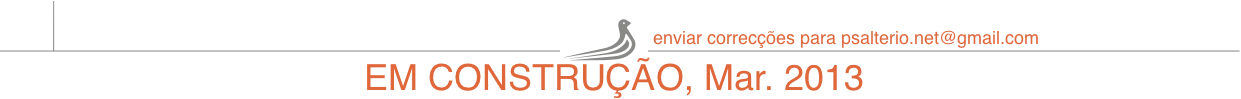
\includegraphics{_images/bkground_page_bottom.png}
}}





% this includes all the guitar tabs that may be needed
% must complete all the chords used in psalterio

% Cb chords

% C chords
\def \gtabCb{\gtab{Cb}{X32010:X32010}}
\def \gtabC{\gtab{C}{X32010:032010}}
\def \gtabCm{\gtab{Cm}{3:113321:004320}}

\def \gtabCsharpSusFour{\gtab{C\#sus4}{4:XX3341:XX2341}}

% Db chords

% D chords
\def \gtabD{\gtab{D}{X00232:000132}}
\def \gtabDm{\gtab{Dm}{X00231:000231}}
\def \gtabDfour{\gtab{D4}{X00233:000134}}
\def \gtabDseven{\gtab{D7}{X00212:000213}}
\def \gtabDsevenPlus{\gtab{D7+}{X00222:000111}}

% D#/Eb chords
\def \gtabDsharp{\gtab{D\#}{2:XX0232:000132}}

% E chords
\def \gtabE{\gtab{E}{022100:023100}}
\def \gtabEseven{\gtab{E}{020100:020100}}

\def \gtabEm{\gtab{Em}{022000:012000}}
\def \gtabEmSeven{\gtab{Em7}{022030:012040}}

% Gb chords

% F chords
\def \gtabF{\gtab{F}{1:133211:034200}}
\def \gtabFm{\gtab{Fm}{1:133111:034000}}


% F# chords
\def \gtabFsharpMinor{\gtab{F\#m}{2:133111:034000}}
\def \gtabFsharpMinorSeven{\gtab{F\#m7}{2:131131:030040}}

% Gb chords

% G chords
\def \gtabG{\gtab{G}{320033:210034}}
\def \gtabGseven{\gtab{G7}{320001:320001}}
\def \gtabGfret{\gtab{(G)}{3:133211:034200}}
\def \gtabGm{\gtab{Gm}{3:133111:034000}}


% G# / Ab chords

% A chords
\def \gtabA{\gtab{A}{X02220:001230}}
\def \gtabAm{\gtab{Am}{X02210:002310}}
\def \gtabAmSeven{\gtab{Am7}{X02010:002010}}
\def \gtabAfour{\gtab{A4}{X02230:001230}}
\def \gtabAseven{\gtab{A7}{X02020:001030}}

% Bb chords
\def \gtabBb{\gtab{Bb}{X13331}}

% B chords
\def \gtabB{\gtab{B}{X13331:003210}}
\def \gtabBm{\gtab{Bm}{X13321:003420}}
\def \gtabBmSeven{\gtab{Bm7}{X13121:003020}}



% after any { or } at the end of a line inside the macro definition add %, otherwise you'll get an extra space
\newcommand{\guitarTab}[1]{%
\ifstrequal{#1}{Cb}      {\gtab{Cb}{X32010:X32010}      }{}%
\ifstrequal{#1}{C}        { \gtab{C}{X32010:032010}       }{}%
%
%G
%
\ifstrequal{#1}{G}       { \gtab{G}{320033:210034}       }{}%
\ifstrequal{#1}{G7}     { \gtab{G7}{320001:320001}     }{}%
\ifstrequal{#1}{Gfret}  { \gtab{G}{3:133211:034200}    }{}%
\ifstrequal{#1}{Gm}    { \gtab{Gm}{3:133111:034000}  }{}%
} %end \newcommand{\gtab}

%muda aqui o numero da musica em que estas a trabalhar
%\def \selectSong{114}

\providebool{gchords}
\setbool{gchords}{true}

% set guitar chords vertical space separation with lyrics
\def \gchordsVspace{5 mm}

\begin{document}
	
	
	\AddToShipoutPicture*{\BottomPic}
	
	\begin{songs}{}
	
	%format file
	%
%Font Sizes
%
%\tiny
%\scriptsize
%\footnotesize
%\small
%\normalsize
%\large
%\Large
%\LARGE
%\huge
%\Huge


%\renewcommand{\thesongnum}{A\arabic{songnum}}
\renewcommand{\printsongnum}[1]{\sffamily\bfseries\huge\MakeUppercase#1}
\setlength{\songnumwidth}{2cm} % box width
%\renewcommand{\snumbgcolor}{white}

%change font for Title
\renewcommand{\stitlefont}{\sffamily\bfseries\huge\MakeUppercase} %song title

%remove verse numbers
%\noversenumbers 
% make left separation
\setlength{\versenumwidth}{2.0cm}

%verse separations
%\versesep=15pt
%\afterpreludeskip=2pt
%\beforepostludeskip=2pt
%\baselineadj=10pt

% separation between chords and lyrics
\renewcommand{\clineparams}{ 
\baselineskip=10pt 
%\lineskiplimit=2pt 
%\lineskip=5pt
}

% change font for lyrics
%\renewcommand{\lyricfont}{\sffamily}
%\renewcommand{\lyricfont}{\sffamily\small}
\renewcommand{\lyricfont}{\sffamily\large}
%\renewcommand{\chorusfont}{\sffamily}
\renewcommand{\chorusfont}{\sffamily\large}

%change the Chords formatting
\renewcommand{\printchord}[1]{\sffamily\color{red}\it\normalsize#1}

%check http://www.tug.org/pracjourn/2006-1/schmidt/schmidt.pdf


%\renewcommand{\songauthors}[1]{tete #1}


%\renewcommand{\extendpostlude}
%{ \songcopyright\ \songlicense\unskip \ Used with permission.}

\setlength{\cbarwidth}{0pt}
\setlength{\sbarheight}{0pt}

% music anf lyrics by
\newcommand{\musicLyricsBy}{} 
\newsongkey{mlby}{\def\musicLyricsBy{}}
                 {\def\musicLyricsBy{\sffamily\it\small letra e música por #1\par}}

% music anf lyrics by
\newcommand{\musicby}{} 
\newsongkey{music}{\def\musicby{}}
                 {\def\musicby{\sffamily\it\small música: #1\par}}

% music anf lyrics by
\newcommand{\lyricsby}{} 
\newsongkey{lyrics}{\def\lyricsby{}}
                 {\def\lyricsby{\sffamily\it\small letra: #1\par}}

%\renewcommand{\sharpsymbol}{\ensuremath{^\sharp}}
\renewcommand{\extendprelude}{
  \showrefs\showauthors 
  %{\bfseries\musicLyricsBy}
  {\bfseries\musicby}
  {\bfseries\lyricsby}
}

\def \gtabsOn{1}
	
%%%%%%%%%%%%%%%%%%%%%%%%%%%%%%%%%%%%%%%%%%%%%%%%%%%%%%%%%%%%%%%%%%%%%%%%%%%
% set song number
%%%%%%%%%%%%%%%%%%%%%%%%%%%%%%%%%%%%%%%%%%%%%%%%%%%%%%%%%%%%%%%%%%%%%%%%%%%
\setcounter{songnum}{4}       % song number
%%%%%%%%%%%%%%%%%%%%%%%%%%%%%%%%%%%%%%%%%%%%%%%%%%%%%%%%%%%%%%%%%%%%%%%%%%%
% begin song latex formating, set the title and other info
%%%%%%%%%%%%%%%%%%%%%%%%%%%%%%%%%%%%%%%%%%%%%%%%%%%%%%%%%%%%%%%%%%%%%%%%%%%
\beginsong{Hino dos Companheiros}[            % song title ...
    %mlby={},                           % music and lyric by
    %sr={Revelation 5:13},        % bible verse
    %cr={Public domain.},         % licence
    %arr={my},                          % arrangement by
    index={Hino dos Companheiros}]               % index title ...	
%%%%%%%%%%%%%%%%%%%%%%%%%%%%%%%%%%%%%%%%%%%%%%%%%%%%%%%%%%%%%%%%%%%%%%%%%%%
% verse #1
%%%%%%%%%%%%%%%%%%%%%%%%%%%%%%%%%%%%%%%%%%%%%%%%%%%%%%%%%%%%%%%%%%%%%%%%%%%
\beginverse                       % start verse
\[A]Vigi\[D]ai, \[A]Jov\[F#m]ens v\[E]enc\[A]ei!
\[D]Do mundo \[A]os v\[F#m]is enga\[Bm]nos\[E].
\[A]Seja a Bi\[D]blia \[E]a \[F#m]voss\[E]a l\[A]ei
\[D]No verd\[A]or dos vo\[F#m]ssos \[E]ano\[A]s.
\endverse                         % end verse
%%%%%%%%%%%%%%%%%%%%%%%%%%%%%%%%%%%%%%%%%%%%%%%%%%%%%%%%%%%%%%%%%%%%%%%%%%%
% verse #2
%%%%%%%%%%%%%%%%%%%%%%%%%%%%%%%%%%%%%%%%%%%%%%%%%%%%%%%%%%%%%%%%%%%%%%%%%%%
\beginverse                       % start verse
\[A]Jovens \[D]cren\[A]tes, \[F#m]des\[E]pert\[A]ai!
\[D]E, enquanto e \[A]tem\[F#m]po ain\[Bm]da\[E],
\[A]Com fe vi\[D]va \[E]proc\[F#m]lam\[A]ai
\[D]De Je\[A]sus a bre\[F#m]ve \[E]vind\[A]a.
\endverse                         % start verse
%%%%%%%%%%%%%%%%%%%%%%%%%%%%%%%%%%%%%%%%%%%%%%%%%%%%%%%%%%%%%%%%%%%%%%%%%%%
% print guitar tabs used in this song
%%%%%%%%%%%%%%%%%%%%%%%%%%%%%%%%%%%%%%%%%%%%%%%%%%%%%%%%%%%%%%%%%%%%%%%%%%%
\ifbool{gchords}{                 % if the guitar chords are to be printed
\vspace{\gchordsVspace}           % set a vertical space of 10 pt 
\gtabC
\gtabF
%\gtabGseven
\gtabFsharpMinor
\gtabBm
}                                 % end if
%%%%%%%%%%%%%%%%%%%%%%%%%%%%%%%%%%%%%%%%%%%%%%%%%%%%%%%%%%%%%%%%%%%%%%%%%%%
% end song latex formating
%%%%%%%%%%%%%%%%%%%%%%%%%%%%%%%%%%%%%%%%%%%%%%%%%%%%%%%%%%%%%%%%%%%%%%%%%%%
\endsong                          % end song
%	 %lilypond-book --output=out --pdf  106single.tex
	 %\lilypondfile[]{E_101.ly}
	
\end{document}
	% percentagem é comentário
% 1 - \setcounter{songnum}{0} - numero da musica
% 2 - \beginsong{Hino Missionario Voluntario}[ - título da música
% 3 -  index={Hino Missionario Voluntario}] - entrada do indice da musica
% 4 - \beginverse , depois desta linha adicionar a letra
%%%%%%%%%%%%%%%%%%%%%%%%%%%%%%%%%%%%%%%%%%%%%%%%%%%%%%%%%%%%%%%%%%%%%%%%%%%
% this has all the necessary packages and formatting for the document
%%%%%%%%%%%%%%%%%%%%%%%%%%%%%%%%%%%%%%%%%%%%%%%%%%%%%%%%%%%%%%%%%%%%%%%%%%%
%\def \includeFolder{../_include}

% this has all the necessary packages and formatting for the document
\documentclass[10pt,a5paper]{article}

%define include folder
\def \includeFolder{_include}

%packages
\usepackage[left=1cm,right=1cm,top=1cm,bottom=1cm]{geometry}

\usepackage[chorded]{\includeFolder/psalterio} %must check the licence to change the name of the sty file!!!
%\usepackage[chorded]{resources/songs-old} %must check the licence to change the name of the sty file!!!

\usepackage[utf8]{inputenc}

\usepackage{graphicx}
\usepackage{wrapfig}
\usepackage{wallpaper}
\usepackage{color}
\usepackage{eso-pic} %for background pictures
\usepackage[bookmarks]{hyperref} 
%\usepackage{ifthen} %etoolbox is more up to date
\usepackage{etoolbox}


%\usepackage[xetex]{graphicx}
%\usepackage{fontspec,xunicode}
%\defaultfontfeatures{Mapping=tex-text,Scale=MatchLowercase}
%\setmainfont[Scale=.95]{Times}
%\setmonofont{Lucida Sans Typewriter}

%\usepackage[portuguese]{babel}
%\usepackage[latin1]{inputenc}
%\usepackage[utf8]{inputenc}
%\usepackage[T1]{fontenc}
%\usepackage[scaled]{uarial}
%\usepackage{helvet}
%\renewcommand{\familydefault}{\sfdefault}

%this removes the page number
\thispagestyle{empty}
\pagestyle{empty}
\songcolumns{1}

\parindent 0pt

%add background picture
\newcommand\BackgroundPic{
\put(0,0){
\parbox[b][\paperheight]{\paperwidth}{%
\vfill
\centering

\includegraphics[width=\paperwidth,height=\paperheight,
keepaspectratio]{logo.png}%
\vfill
}}}

\newcommand\BottomPic{
\put(0,0){
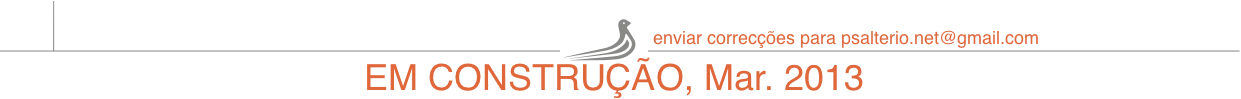
\includegraphics{_images/bkground_page_bottom.png}
}}





% this includes all the guitar tabs that may be needed
% must complete all the chords used in psalterio

% Cb chords

% C chords
\def \gtabCb{\gtab{Cb}{X32010:X32010}}
\def \gtabC{\gtab{C}{X32010:032010}}
\def \gtabCm{\gtab{Cm}{3:113321:004320}}

\def \gtabCsharpSusFour{\gtab{C\#sus4}{4:XX3341:XX2341}}

% Db chords

% D chords
\def \gtabD{\gtab{D}{X00232:000132}}
\def \gtabDm{\gtab{Dm}{X00231:000231}}
\def \gtabDfour{\gtab{D4}{X00233:000134}}
\def \gtabDseven{\gtab{D7}{X00212:000213}}
\def \gtabDsevenPlus{\gtab{D7+}{X00222:000111}}

% D#/Eb chords
\def \gtabDsharp{\gtab{D\#}{2:XX0232:000132}}

% E chords
\def \gtabE{\gtab{E}{022100:023100}}
\def \gtabEseven{\gtab{E}{020100:020100}}

\def \gtabEm{\gtab{Em}{022000:012000}}
\def \gtabEmSeven{\gtab{Em7}{022030:012040}}

% Gb chords

% F chords
\def \gtabF{\gtab{F}{1:133211:034200}}
\def \gtabFm{\gtab{Fm}{1:133111:034000}}


% F# chords
\def \gtabFsharpMinor{\gtab{F\#m}{2:133111:034000}}
\def \gtabFsharpMinorSeven{\gtab{F\#m7}{2:131131:030040}}

% Gb chords

% G chords
\def \gtabG{\gtab{G}{320033:210034}}
\def \gtabGseven{\gtab{G7}{320001:320001}}
\def \gtabGfret{\gtab{(G)}{3:133211:034200}}
\def \gtabGm{\gtab{Gm}{3:133111:034000}}


% G# / Ab chords

% A chords
\def \gtabA{\gtab{A}{X02220:001230}}
\def \gtabAm{\gtab{Am}{X02210:002310}}
\def \gtabAmSeven{\gtab{Am7}{X02010:002010}}
\def \gtabAfour{\gtab{A4}{X02230:001230}}
\def \gtabAseven{\gtab{A7}{X02020:001030}}

% Bb chords
\def \gtabBb{\gtab{Bb}{X13331}}

% B chords
\def \gtabB{\gtab{B}{X13331:003210}}
\def \gtabBm{\gtab{Bm}{X13321:003420}}
\def \gtabBmSeven{\gtab{Bm7}{X13121:003020}}



% after any { or } at the end of a line inside the macro definition add %, otherwise you'll get an extra space
\newcommand{\guitarTab}[1]{%
\ifstrequal{#1}{Cb}      {\gtab{Cb}{X32010:X32010}      }{}%
\ifstrequal{#1}{C}        { \gtab{C}{X32010:032010}       }{}%
%
%G
%
\ifstrequal{#1}{G}       { \gtab{G}{320033:210034}       }{}%
\ifstrequal{#1}{G7}     { \gtab{G7}{320001:320001}     }{}%
\ifstrequal{#1}{Gfret}  { \gtab{G}{3:133211:034200}    }{}%
\ifstrequal{#1}{Gm}    { \gtab{Gm}{3:133111:034000}  }{}%
} %end \newcommand{\gtab}

%muda aqui o numero da musica em que estas a trabalhar
%\def \selectSong{114}

\providebool{gchords}
\setbool{gchords}{true}

% set guitar chords vertical space separation with lyrics
\def \gchordsVspace{5 mm}

\begin{document}
	
	
	\AddToShipoutPicture*{\BottomPic}
	
	\begin{songs}{}
	
	%format file
	%
%Font Sizes
%
%\tiny
%\scriptsize
%\footnotesize
%\small
%\normalsize
%\large
%\Large
%\LARGE
%\huge
%\Huge


%\renewcommand{\thesongnum}{A\arabic{songnum}}
\renewcommand{\printsongnum}[1]{\sffamily\bfseries\huge\MakeUppercase#1}
\setlength{\songnumwidth}{2cm} % box width
%\renewcommand{\snumbgcolor}{white}

%change font for Title
\renewcommand{\stitlefont}{\sffamily\bfseries\huge\MakeUppercase} %song title

%remove verse numbers
%\noversenumbers 
% make left separation
\setlength{\versenumwidth}{2.0cm}

%verse separations
%\versesep=15pt
%\afterpreludeskip=2pt
%\beforepostludeskip=2pt
%\baselineadj=10pt

% separation between chords and lyrics
\renewcommand{\clineparams}{ 
\baselineskip=10pt 
%\lineskiplimit=2pt 
%\lineskip=5pt
}

% change font for lyrics
%\renewcommand{\lyricfont}{\sffamily}
%\renewcommand{\lyricfont}{\sffamily\small}
\renewcommand{\lyricfont}{\sffamily\large}
%\renewcommand{\chorusfont}{\sffamily}
\renewcommand{\chorusfont}{\sffamily\large}

%change the Chords formatting
\renewcommand{\printchord}[1]{\sffamily\color{red}\it\normalsize#1}

%check http://www.tug.org/pracjourn/2006-1/schmidt/schmidt.pdf


%\renewcommand{\songauthors}[1]{tete #1}


%\renewcommand{\extendpostlude}
%{ \songcopyright\ \songlicense\unskip \ Used with permission.}

\setlength{\cbarwidth}{0pt}
\setlength{\sbarheight}{0pt}

% music anf lyrics by
\newcommand{\musicLyricsBy}{} 
\newsongkey{mlby}{\def\musicLyricsBy{}}
                 {\def\musicLyricsBy{\sffamily\it\small letra e música por #1\par}}

% music anf lyrics by
\newcommand{\musicby}{} 
\newsongkey{music}{\def\musicby{}}
                 {\def\musicby{\sffamily\it\small música: #1\par}}

% music anf lyrics by
\newcommand{\lyricsby}{} 
\newsongkey{lyrics}{\def\lyricsby{}}
                 {\def\lyricsby{\sffamily\it\small letra: #1\par}}

%\renewcommand{\sharpsymbol}{\ensuremath{^\sharp}}
\renewcommand{\extendprelude}{
  \showrefs\showauthors 
  %{\bfseries\musicLyricsBy}
  {\bfseries\musicby}
  {\bfseries\lyricsby}
}

\def \gtabsOn{1}
	
%%%%%%%%%%%%%%%%%%%%%%%%%%%%%%%%%%%%%%%%%%%%%%%%%%%%%%%%%%%%%%%%%%%%%%%%%%%
% set song number
%%%%%%%%%%%%%%%%%%%%%%%%%%%%%%%%%%%%%%%%%%%%%%%%%%%%%%%%%%%%%%%%%%%%%%%%%%%
\setcounter{songnum}{5}       % song number
%%%%%%%%%%%%%%%%%%%%%%%%%%%%%%%%%%%%%%%%%%%%%%%%%%%%%%%%%%%%%%%%%%%%%%%%%%%
% begin song latex formating, set the title and other info
%%%%%%%%%%%%%%%%%%%%%%%%%%%%%%%%%%%%%%%%%%%%%%%%%%%%%%%%%%%%%%%%%%%%%%%%%%%
\beginsong{Hino do Missionário Voluntário}[            % song title ...
    %mlby={},                           % music and lyric by
    %sr={Revelation 5:13},        % bible verse
    %cr={Public domain.},         % licence
    %arr={my},                          % arrangement by
    index={Hino do Missionário Voluntário}]               % index title ...	
%%%%%%%%%%%%%%%%%%%%%%%%%%%%%%%%%%%%%%%%%%%%%%%%%%%%%%%%%%%%%%%%%%%%%%%%%%%
% verse #1
%%%%%%%%%%%%%%%%%%%%%%%%%%%%%%%%%%%%%%%%%%%%%%%%%%%%%%%%%%%%%%%%%%%%%%%%%%%
\beginverse                       % start verse
\[C]O Mi\[C69+]ssionari\[C]o voluntário, Cristo ja vos cham\[G7]a a\[D7]o co\[G7]mbate con\[D7]tra \[G7]o \[D7]mal\[G7].
Milh\[C]oes e\[E]m tr\[Am]eva\[C7]s clamam po\[F]r socorro, Ide, o mo\[C]ci\[C69+]dade v\[C]aronil, leal.\[G7] \[C]
\endverse                         % end verse
%%%%%%%%%%%%%%%%%%%%%%%%%%%%%%%%%%%%%%%%%%%%%%%%%%%%%%%%%%%%%%%%%%%%%%%%%%%
% chorus #1
%%%%%%%%%%%%%%%%%%%%%%%%%%%%%%%%%%%%%%%%%%%%%%%%%%%%%%%%%%%%%%%%%%%%%%%%%%%
\beginchorus                       % start verse
\[C]O mocidade adventista! Vamos sair a trabalhar\[G7]
Salvar as almas que estao perdidas, leva-las ao celeste lar.\[C] 
Nao ha tarefa mais gloriosa que este Evangelho anunciar.\[F]
O mocid\[C]ade brava e ditosa! Jesus ord\[F]ena tra\[G7]balhar!\[C]
\endchorus                         % start verse

%%%%%%%%%%%%%%%%%%%%%%%%%%%%%%%%%%%%%%%%%%%%%%%%%%%%%%%%%%%%%%%%%%%%%%%%%%%
% verse #2
%%%%%%%%%%%%%%%%%%%%%%%%%%%%%%%%%%%%%%%%%%%%%%%%%%%%%%%%%%%%%%%%%%%%%%%%%%%
\beginverse                       % start verse
\[C]O mun\[C69+]do inteiro \[C] jaz em densas trevas do peca\[G7]do v\[D7]il, ca\[G7]ido em \[D7]scuri\[G7]d\[D7]ao\[G7].
Aqu\[C]i be\[E]m p\[Am]ert\[C7]o existem pre\[F]ciosas almas es\[C]pera\[C69+]ndo quem lhes d\[C]e a mao.\[G7] \[C]
\endverse                         % end verse

%%%%%%%%%%%%%%%%%%%%%%%%%%%%%%%%%%%%%%%%%%%%%%%%%%%%%%%%%%%%%%%%%%%%%%%%%%%
% verse #3
%%%%%%%%%%%%%%%%%%%%%%%%%%%%%%%%%%%%%%%%%%%%%%%%%%%%%%%%%%%%%%%%%%%%%%%%%%%
\beginverse                       % start verse
\[C]Voan\[C69+]do pelo \[C]espaco esta mensagem de Jesus\[G7] ir\[D7]a a\[G7]s alm\[D7]as conv\[G7]ert\[D7]er\[G7].
O v\[C]al\[E]or\[Am]os\[C7]a mocida\[F]de brava, sem\[C]pre unidos va\[C69+]mos todos comb\[C]ater.\[G7] \[C]
\endverse                         % end verse

%%%%%%%%%%%%%%%%%%%%%%%%%%%%%%%%%%%%%%%%%%%%%%%%%%%%%%%%%%%%%%%%%%%%%%%%%%%
% verse #4
%%%%%%%%%%%%%%%%%%%%%%%%%%%%%%%%%%%%%%%%%%%%%%%%%%%%%%%%%%%%%%%%%%%%%%%%%%%
\beginverse                       % start verse
\[C]Ao to\[C69+]que de cla\[C]rim as multidoes arrependi\[G7]da\[D7]s a Je\[G7]sus hao\[D7] de a\[G7]ceit\[D7]ar\[G7].
Cur\[C]ai\[C6], pregai\[Am] es\[C7]te Evan\[F]gelho eterno, pois\[C], anunciai:\[C69+] que Cristo vai vo\[C]ltar.\[G7] \[C]
\endverse                         % end verse

%%%%%%%%%%%%%%%%%%%%%%%%%%%%%%%%%%%%%%%%%%%%%%%%%%%%%%%%%%%%%%%%%%%%%%%%%%%
% verse #5
%%%%%%%%%%%%%%%%%%%%%%%%%%%%%%%%%%%%%%%%%%%%%%%%%%%%%%%%%%%%%%%%%%%%%%%%%%%
\beginverse                       % start verse
\[C]O valorosa mocidade! Ide, aos vizinhos, de Jesus\[G7]
Pelos caminhos, pelos valados, levar-lhes a celeste luz.\[C]
Nao ha tarefa mais gloriosa que este Evangelho anunciar.\[F]
O mocid\[C]ade brava e ditosa! Unidos \[F]vamos tra\[G7]balhar!\[C]
\endverse                         % end verse

%%%%%%%%%%%%%%%%%%%%%%%%%%%%%%%%%%%%%%%%%%%%%%%%%%%%%%%%%%%%%%%%%%%%%%%%%%%
% print guitar tabs used in this song
%%%%%%%%%%%%%%%%%%%%%%%%%%%%%%%%%%%%%%%%%%%%%%%%%%%%%%%%%%%%%%%%%%%%%%%%%%%
\ifbool{gchords}{                 % if the guitar chords are to be printed
\vspace{\gchordsVspace}           % set a vertical space of 10 pt 

\gtabC
\gtabF
%\gtabGseven
\gtabFsharpMinor
\gtabBm

}                                 % end if

%%%%%%%%%%%%%%%%%%%%%%%%%%%%%%%%%%%%%%%%%%%%%%%%%%%%%%%%%%%%%%%%%%%%%%%%%%%
% end song latex formating
%%%%%%%%%%%%%%%%%%%%%%%%%%%%%%%%%%%%%%%%%%%%%%%%%%%%%%%%%%%%%%%%%%%%%%%%%%%
\endsong                          % end song
%	 %lilypond-book --output=out --pdf  106single.tex
	 %\lilypondfile[]{E_101.ly}
	
\end{document}
	% percentagem é comentário
% 1 - \setcounter{songnum}{0} - numero da musica
% 2 - \beginsong{Hino do Projecto/70}[ - título da música
% 3 -  index={Hino do Projecto/70}] - entrada do indice da musica
% 4 - \beginverse , depois desta linha adicionar a letra
%%%%%%%%%%%%%%%%%%%%%%%%%%%%%%%%%%%%%%%%%%%%%%%%%%%%%%%%%%%%%%%%%%%%%%%%%%%
% this has all the necessary packages and formatting for the document
%%%%%%%%%%%%%%%%%%%%%%%%%%%%%%%%%%%%%%%%%%%%%%%%%%%%%%%%%%%%%%%%%%%%%%%%%%%
%\def \includeFolder{../_include}

% this has all the necessary packages and formatting for the document
\documentclass[10pt,a5paper]{article}

%define include folder
\def \includeFolder{_include}

%packages
\usepackage[left=1cm,right=1cm,top=1cm,bottom=1cm]{geometry}

\usepackage[chorded]{\includeFolder/psalterio} %must check the licence to change the name of the sty file!!!
%\usepackage[chorded]{resources/songs-old} %must check the licence to change the name of the sty file!!!

\usepackage[utf8]{inputenc}

\usepackage{graphicx}
\usepackage{wrapfig}
\usepackage{wallpaper}
\usepackage{color}
\usepackage{eso-pic} %for background pictures
\usepackage[bookmarks]{hyperref} 
%\usepackage{ifthen} %etoolbox is more up to date
\usepackage{etoolbox}


%\usepackage[xetex]{graphicx}
%\usepackage{fontspec,xunicode}
%\defaultfontfeatures{Mapping=tex-text,Scale=MatchLowercase}
%\setmainfont[Scale=.95]{Times}
%\setmonofont{Lucida Sans Typewriter}

%\usepackage[portuguese]{babel}
%\usepackage[latin1]{inputenc}
%\usepackage[utf8]{inputenc}
%\usepackage[T1]{fontenc}
%\usepackage[scaled]{uarial}
%\usepackage{helvet}
%\renewcommand{\familydefault}{\sfdefault}

%this removes the page number
\thispagestyle{empty}
\pagestyle{empty}
\songcolumns{1}

\parindent 0pt

%add background picture
\newcommand\BackgroundPic{
\put(0,0){
\parbox[b][\paperheight]{\paperwidth}{%
\vfill
\centering

\includegraphics[width=\paperwidth,height=\paperheight,
keepaspectratio]{logo.png}%
\vfill
}}}

\newcommand\BottomPic{
\put(0,0){
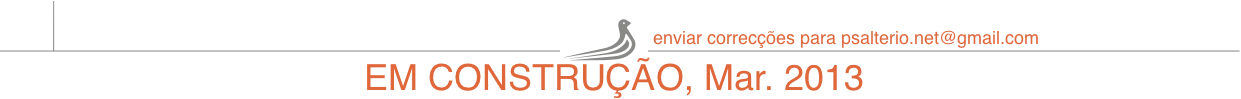
\includegraphics{_images/bkground_page_bottom.png}
}}





% this includes all the guitar tabs that may be needed
% must complete all the chords used in psalterio

% Cb chords

% C chords
\def \gtabCb{\gtab{Cb}{X32010:X32010}}
\def \gtabC{\gtab{C}{X32010:032010}}
\def \gtabCm{\gtab{Cm}{3:113321:004320}}

\def \gtabCsharpSusFour{\gtab{C\#sus4}{4:XX3341:XX2341}}

% Db chords

% D chords
\def \gtabD{\gtab{D}{X00232:000132}}
\def \gtabDm{\gtab{Dm}{X00231:000231}}
\def \gtabDfour{\gtab{D4}{X00233:000134}}
\def \gtabDseven{\gtab{D7}{X00212:000213}}
\def \gtabDsevenPlus{\gtab{D7+}{X00222:000111}}

% D#/Eb chords
\def \gtabDsharp{\gtab{D\#}{2:XX0232:000132}}

% E chords
\def \gtabE{\gtab{E}{022100:023100}}
\def \gtabEseven{\gtab{E}{020100:020100}}

\def \gtabEm{\gtab{Em}{022000:012000}}
\def \gtabEmSeven{\gtab{Em7}{022030:012040}}

% Gb chords

% F chords
\def \gtabF{\gtab{F}{1:133211:034200}}
\def \gtabFm{\gtab{Fm}{1:133111:034000}}


% F# chords
\def \gtabFsharpMinor{\gtab{F\#m}{2:133111:034000}}
\def \gtabFsharpMinorSeven{\gtab{F\#m7}{2:131131:030040}}

% Gb chords

% G chords
\def \gtabG{\gtab{G}{320033:210034}}
\def \gtabGseven{\gtab{G7}{320001:320001}}
\def \gtabGfret{\gtab{(G)}{3:133211:034200}}
\def \gtabGm{\gtab{Gm}{3:133111:034000}}


% G# / Ab chords

% A chords
\def \gtabA{\gtab{A}{X02220:001230}}
\def \gtabAm{\gtab{Am}{X02210:002310}}
\def \gtabAmSeven{\gtab{Am7}{X02010:002010}}
\def \gtabAfour{\gtab{A4}{X02230:001230}}
\def \gtabAseven{\gtab{A7}{X02020:001030}}

% Bb chords
\def \gtabBb{\gtab{Bb}{X13331}}

% B chords
\def \gtabB{\gtab{B}{X13331:003210}}
\def \gtabBm{\gtab{Bm}{X13321:003420}}
\def \gtabBmSeven{\gtab{Bm7}{X13121:003020}}



% after any { or } at the end of a line inside the macro definition add %, otherwise you'll get an extra space
\newcommand{\guitarTab}[1]{%
\ifstrequal{#1}{Cb}      {\gtab{Cb}{X32010:X32010}      }{}%
\ifstrequal{#1}{C}        { \gtab{C}{X32010:032010}       }{}%
%
%G
%
\ifstrequal{#1}{G}       { \gtab{G}{320033:210034}       }{}%
\ifstrequal{#1}{G7}     { \gtab{G7}{320001:320001}     }{}%
\ifstrequal{#1}{Gfret}  { \gtab{G}{3:133211:034200}    }{}%
\ifstrequal{#1}{Gm}    { \gtab{Gm}{3:133111:034000}  }{}%
} %end \newcommand{\gtab}

%muda aqui o numero da musica em que estas a trabalhar
%\def \selectSong{114}

\providebool{gchords}
\setbool{gchords}{true}

% set guitar chords vertical space separation with lyrics
\def \gchordsVspace{5 mm}

\begin{document}
	
	
	\AddToShipoutPicture*{\BottomPic}
	
	\begin{songs}{}
	
	%format file
	%
%Font Sizes
%
%\tiny
%\scriptsize
%\footnotesize
%\small
%\normalsize
%\large
%\Large
%\LARGE
%\huge
%\Huge


%\renewcommand{\thesongnum}{A\arabic{songnum}}
\renewcommand{\printsongnum}[1]{\sffamily\bfseries\huge\MakeUppercase#1}
\setlength{\songnumwidth}{2cm} % box width
%\renewcommand{\snumbgcolor}{white}

%change font for Title
\renewcommand{\stitlefont}{\sffamily\bfseries\huge\MakeUppercase} %song title

%remove verse numbers
%\noversenumbers 
% make left separation
\setlength{\versenumwidth}{2.0cm}

%verse separations
%\versesep=15pt
%\afterpreludeskip=2pt
%\beforepostludeskip=2pt
%\baselineadj=10pt

% separation between chords and lyrics
\renewcommand{\clineparams}{ 
\baselineskip=10pt 
%\lineskiplimit=2pt 
%\lineskip=5pt
}

% change font for lyrics
%\renewcommand{\lyricfont}{\sffamily}
%\renewcommand{\lyricfont}{\sffamily\small}
\renewcommand{\lyricfont}{\sffamily\large}
%\renewcommand{\chorusfont}{\sffamily}
\renewcommand{\chorusfont}{\sffamily\large}

%change the Chords formatting
\renewcommand{\printchord}[1]{\sffamily\color{red}\it\normalsize#1}

%check http://www.tug.org/pracjourn/2006-1/schmidt/schmidt.pdf


%\renewcommand{\songauthors}[1]{tete #1}


%\renewcommand{\extendpostlude}
%{ \songcopyright\ \songlicense\unskip \ Used with permission.}

\setlength{\cbarwidth}{0pt}
\setlength{\sbarheight}{0pt}

% music anf lyrics by
\newcommand{\musicLyricsBy}{} 
\newsongkey{mlby}{\def\musicLyricsBy{}}
                 {\def\musicLyricsBy{\sffamily\it\small letra e música por #1\par}}

% music anf lyrics by
\newcommand{\musicby}{} 
\newsongkey{music}{\def\musicby{}}
                 {\def\musicby{\sffamily\it\small música: #1\par}}

% music anf lyrics by
\newcommand{\lyricsby}{} 
\newsongkey{lyrics}{\def\lyricsby{}}
                 {\def\lyricsby{\sffamily\it\small letra: #1\par}}

%\renewcommand{\sharpsymbol}{\ensuremath{^\sharp}}
\renewcommand{\extendprelude}{
  \showrefs\showauthors 
  %{\bfseries\musicLyricsBy}
  {\bfseries\musicby}
  {\bfseries\lyricsby}
}

\def \gtabsOn{1}
	

%%%%%%%%%%%%%%%%%%%%%%%%%%%%%%%%%%%%%%%%%%%%%%%%%%%%%%%%%%%%%%%%%%%%%%%%%%%
% set song number
%%%%%%%%%%%%%%%%%%%%%%%%%%%%%%%%%%%%%%%%%%%%%%%%%%%%%%%%%%%%%%%%%%%%%%%%%%%
\setcounter{songnum}{6}       % song number

%%%%%%%%%%%%%%%%%%%%%%%%%%%%%%%%%%%%%%%%%%%%%%%%%%%%%%%%%%%%%%%%%%%%%%%%%%%
% begin song latex formating, set the title and other info
%%%%%%%%%%%%%%%%%%%%%%%%%%%%%%%%%%%%%%%%%%%%%%%%%%%%%%%%%%%%%%%%%%%%%%%%%%%
\beginsong{Hino do Projecto 70}[            % song title ...
    %mlby={},                           % music and lyric by
    %sr={Revelation 5:13},        % bible verse
    %cr={Public domain.},         % licence
    %arr={my},                          % arrangement by
    index={Hino do Projecto 70}]               % index title ...	
%%%%%%%%%%%%%%%%%%%%%%%%%%%%%%%%%%%%%%%%%%%%%%%%%%%%%%%%%%%%%%%%%%%%%%%%%%%
% verse #1
%%%%%%%%%%%%%%%%%%%%%%%%%%%%%%%%%%%%%%%%%%%%%%%%%%%%%%%%%%%%%%%%%%%%%%%%%%%
\beginverse                       % start verse
\[F]Olhando a Jesus, sigo passo a pa\[C7]sso,
Vivendo o proje\[C7]cto \[C9]em seu\[C] gran\[G7]de \[C7]amor\[F].
Afastar nao me pode, nem m\[F7]esmo o temo\[Bb]r,
Olha\[Bm6]ndo a Jesu\[F]s, sig\[C7]o passo a pa\[F]sso.
\endverse                         % end verse
%%%%%%%%%%%%%%%%%%%%%%%%%%%%%%%%%%%%%%%%%%%%%%%%%%%%%%%%%%%%%%%%%%%%%%%%%%%
% verse #2
%%%%%%%%%%%%%%%%%%%%%%%%%%%%%%%%%%%%%%%%%%%%%%%%%%%%%%%%%%%%%%%%%%%%%%%%%%%
\beginverse                       % start verse
\[F]Se o caminho e estreito, e duro a meu pa\[C7]sso,
Eu vou caminhan\[C7]do\[C9], na\[C] for\[G7]ca do \[C7]amor\[F].\
Afastar nao me pode, nem m\[F7]esmo o temo\[Bb]r,
Olha\[Bm6]ndo a Jesu\[F]s, sig\[C7]o passo a pa\[F]sso.
\endverse                         % start verse
%%%%%%%%%%%%%%%%%%%%%%%%%%%%%%%%%%%%%%%%%%%%%%%%%%%%%%%%%%%%%%%%%%%%%%%%%%%
% print guitar tabs used in this song
%%%%%%%%%%%%%%%%%%%%%%%%%%%%%%%%%%%%%%%%%%%%%%%%%%%%%%%%%%%%%%%%%%%%%%%%%%%
\ifbool{gchords}{                 % if the guitar chords are to be printed
\vspace{\gchordsVspace}           % set a vertical space of 10 pt 
\gtabC
\gtabF
%\gtabGseven
\gtabFsharpMinor
\gtabBm
}                                 % end if
%%%%%%%%%%%%%%%%%%%%%%%%%%%%%%%%%%%%%%%%%%%%%%%%%%%%%%%%%%%%%%%%%%%%%%%%%%%
% end song latex formating
%%%%%%%%%%%%%%%%%%%%%%%%%%%%%%%%%%%%%%%%%%%%%%%%%%%%%%%%%%%%%%%%%%%%%%%%%%%
\endsong                          % end song
%	 %lilypond-book --output=out --pdf  106single.tex
	 %\lilypondfile[]{E_101.ly}
	
\end{document}
	%%%%%%%%%%%%%%%%%%%%%%%%%%%%%%%%%%%%%%%%%%%%%%%%%%%%%%%%%%%%%%%%%%%%%%%%%%%
% this has all the necessary packages and formatting for the document
%%%%%%%%%%%%%%%%%%%%%%%%%%%%%%%%%%%%%%%%%%%%%%%%%%%%%%%%%%%%%%%%%%%%%%%%%%%
%\def \includeFolder{../_include}

% this has all the necessary packages and formatting for the document
\documentclass[10pt,a5paper]{article}

%define include folder
\def \includeFolder{_include}

%packages
\usepackage[left=1cm,right=1cm,top=1cm,bottom=1cm]{geometry}

\usepackage[chorded]{\includeFolder/psalterio} %must check the licence to change the name of the sty file!!!
%\usepackage[chorded]{resources/songs-old} %must check the licence to change the name of the sty file!!!

\usepackage[utf8]{inputenc}

\usepackage{graphicx}
\usepackage{wrapfig}
\usepackage{wallpaper}
\usepackage{color}
\usepackage{eso-pic} %for background pictures
\usepackage[bookmarks]{hyperref} 
%\usepackage{ifthen} %etoolbox is more up to date
\usepackage{etoolbox}


%\usepackage[xetex]{graphicx}
%\usepackage{fontspec,xunicode}
%\defaultfontfeatures{Mapping=tex-text,Scale=MatchLowercase}
%\setmainfont[Scale=.95]{Times}
%\setmonofont{Lucida Sans Typewriter}

%\usepackage[portuguese]{babel}
%\usepackage[latin1]{inputenc}
%\usepackage[utf8]{inputenc}
%\usepackage[T1]{fontenc}
%\usepackage[scaled]{uarial}
%\usepackage{helvet}
%\renewcommand{\familydefault}{\sfdefault}

%this removes the page number
\thispagestyle{empty}
\pagestyle{empty}
\songcolumns{1}

\parindent 0pt

%add background picture
\newcommand\BackgroundPic{
\put(0,0){
\parbox[b][\paperheight]{\paperwidth}{%
\vfill
\centering

\includegraphics[width=\paperwidth,height=\paperheight,
keepaspectratio]{logo.png}%
\vfill
}}}

\newcommand\BottomPic{
\put(0,0){
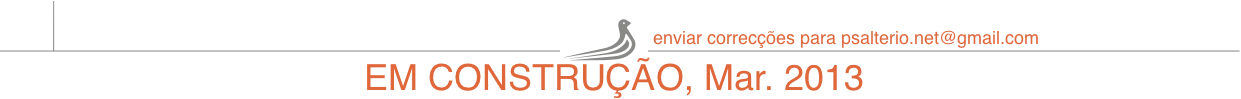
\includegraphics{_images/bkground_page_bottom.png}
}}





% this includes all the guitar tabs that may be needed
% must complete all the chords used in psalterio

% Cb chords

% C chords
\def \gtabCb{\gtab{Cb}{X32010:X32010}}
\def \gtabC{\gtab{C}{X32010:032010}}
\def \gtabCm{\gtab{Cm}{3:113321:004320}}

\def \gtabCsharpSusFour{\gtab{C\#sus4}{4:XX3341:XX2341}}

% Db chords

% D chords
\def \gtabD{\gtab{D}{X00232:000132}}
\def \gtabDm{\gtab{Dm}{X00231:000231}}
\def \gtabDfour{\gtab{D4}{X00233:000134}}
\def \gtabDseven{\gtab{D7}{X00212:000213}}
\def \gtabDsevenPlus{\gtab{D7+}{X00222:000111}}

% D#/Eb chords
\def \gtabDsharp{\gtab{D\#}{2:XX0232:000132}}

% E chords
\def \gtabE{\gtab{E}{022100:023100}}
\def \gtabEseven{\gtab{E}{020100:020100}}

\def \gtabEm{\gtab{Em}{022000:012000}}
\def \gtabEmSeven{\gtab{Em7}{022030:012040}}

% Gb chords

% F chords
\def \gtabF{\gtab{F}{1:133211:034200}}
\def \gtabFm{\gtab{Fm}{1:133111:034000}}


% F# chords
\def \gtabFsharpMinor{\gtab{F\#m}{2:133111:034000}}
\def \gtabFsharpMinorSeven{\gtab{F\#m7}{2:131131:030040}}

% Gb chords

% G chords
\def \gtabG{\gtab{G}{320033:210034}}
\def \gtabGseven{\gtab{G7}{320001:320001}}
\def \gtabGfret{\gtab{(G)}{3:133211:034200}}
\def \gtabGm{\gtab{Gm}{3:133111:034000}}


% G# / Ab chords

% A chords
\def \gtabA{\gtab{A}{X02220:001230}}
\def \gtabAm{\gtab{Am}{X02210:002310}}
\def \gtabAmSeven{\gtab{Am7}{X02010:002010}}
\def \gtabAfour{\gtab{A4}{X02230:001230}}
\def \gtabAseven{\gtab{A7}{X02020:001030}}

% Bb chords
\def \gtabBb{\gtab{Bb}{X13331}}

% B chords
\def \gtabB{\gtab{B}{X13331:003210}}
\def \gtabBm{\gtab{Bm}{X13321:003420}}
\def \gtabBmSeven{\gtab{Bm7}{X13121:003020}}



% after any { or } at the end of a line inside the macro definition add %, otherwise you'll get an extra space
\newcommand{\guitarTab}[1]{%
\ifstrequal{#1}{Cb}      {\gtab{Cb}{X32010:X32010}      }{}%
\ifstrequal{#1}{C}        { \gtab{C}{X32010:032010}       }{}%
%
%G
%
\ifstrequal{#1}{G}       { \gtab{G}{320033:210034}       }{}%
\ifstrequal{#1}{G7}     { \gtab{G7}{320001:320001}     }{}%
\ifstrequal{#1}{Gfret}  { \gtab{G}{3:133211:034200}    }{}%
\ifstrequal{#1}{Gm}    { \gtab{Gm}{3:133111:034000}  }{}%
} %end \newcommand{\gtab}

%muda aqui o numero da musica em que estas a trabalhar
%\def \selectSong{114}

\providebool{gchords}
\setbool{gchords}{true}

% set guitar chords vertical space separation with lyrics
\def \gchordsVspace{5 mm}

\begin{document}
	
	
	\AddToShipoutPicture*{\BottomPic}
	
	\begin{songs}{}
	
	%format file
	%
%Font Sizes
%
%\tiny
%\scriptsize
%\footnotesize
%\small
%\normalsize
%\large
%\Large
%\LARGE
%\huge
%\Huge


%\renewcommand{\thesongnum}{A\arabic{songnum}}
\renewcommand{\printsongnum}[1]{\sffamily\bfseries\huge\MakeUppercase#1}
\setlength{\songnumwidth}{2cm} % box width
%\renewcommand{\snumbgcolor}{white}

%change font for Title
\renewcommand{\stitlefont}{\sffamily\bfseries\huge\MakeUppercase} %song title

%remove verse numbers
%\noversenumbers 
% make left separation
\setlength{\versenumwidth}{2.0cm}

%verse separations
%\versesep=15pt
%\afterpreludeskip=2pt
%\beforepostludeskip=2pt
%\baselineadj=10pt

% separation between chords and lyrics
\renewcommand{\clineparams}{ 
\baselineskip=10pt 
%\lineskiplimit=2pt 
%\lineskip=5pt
}

% change font for lyrics
%\renewcommand{\lyricfont}{\sffamily}
%\renewcommand{\lyricfont}{\sffamily\small}
\renewcommand{\lyricfont}{\sffamily\large}
%\renewcommand{\chorusfont}{\sffamily}
\renewcommand{\chorusfont}{\sffamily\large}

%change the Chords formatting
\renewcommand{\printchord}[1]{\sffamily\color{red}\it\normalsize#1}

%check http://www.tug.org/pracjourn/2006-1/schmidt/schmidt.pdf


%\renewcommand{\songauthors}[1]{tete #1}


%\renewcommand{\extendpostlude}
%{ \songcopyright\ \songlicense\unskip \ Used with permission.}

\setlength{\cbarwidth}{0pt}
\setlength{\sbarheight}{0pt}

% music anf lyrics by
\newcommand{\musicLyricsBy}{} 
\newsongkey{mlby}{\def\musicLyricsBy{}}
                 {\def\musicLyricsBy{\sffamily\it\small letra e música por #1\par}}

% music anf lyrics by
\newcommand{\musicby}{} 
\newsongkey{music}{\def\musicby{}}
                 {\def\musicby{\sffamily\it\small música: #1\par}}

% music anf lyrics by
\newcommand{\lyricsby}{} 
\newsongkey{lyrics}{\def\lyricsby{}}
                 {\def\lyricsby{\sffamily\it\small letra: #1\par}}

%\renewcommand{\sharpsymbol}{\ensuremath{^\sharp}}
\renewcommand{\extendprelude}{
  \showrefs\showauthors 
  %{\bfseries\musicLyricsBy}
  {\bfseries\musicby}
  {\bfseries\lyricsby}
}

\def \gtabsOn{1}
	

%%%%%%%%%%%%%%%%%%%%%%%%%%%%%%%%%%%%%%%%%%%%%%%%%%%%%%%%%%%%%%%%%%%%%%%%%%%
% set song number
%%%%%%%%%%%%%%%%%%%%%%%%%%%%%%%%%%%%%%%%%%%%%%%%%%%%%%%%%%%%%%%%%%%%%%%%%%%
\setcounter{songnum}{7}       % song number

%%%%%%%%%%%%%%%%%%%%%%%%%%%%%%%%%%%%%%%%%%%%%%%%%%%%%%%%%%%%%%%%%%%%%%%%%%%
% begin song latex formating, set the title and other info
%%%%%%%%%%%%%%%%%%%%%%%%%%%%%%%%%%%%%%%%%%%%%%%%%%%%%%%%%%%%%%%%%%%%%%%%%%%
\beginsong{No Espírito Unidos}[            % song title ...
    %mlby={},                           % music and lyric by
    %sr={Revelation 5:13},        % bible verse
    %cr={Public domain.},         % licence
    %arr={my},                          % arrangement by
    index={No Espírito Unidos}]               % index title ...	

%%%%%%%%%%%%%%%%%%%%%%%%%%%%%%%%%%%%%%%%%%%%%%%%%%%%%%%%%%%%%%%%%%%%%%%%%%%
% verse #1
%%%%%%%%%%%%%%%%%%%%%%%%%%%%%%%%%%%%%%%%%%%%%%%%%%%%%%%%%%%%%%%%%%%%%%%%%%%
\beginverse                       % start verse
\[Fm]No Espirito unidos, somos um no Senhor,
No Espi\[Bbm]rito unidos somos \[Fm]um no Senhor,   
E implor\[Bbm]amos que um dia nos u\[Fm]namos no amor.
\endverse                         % end verse

%%%%%%%%%%%%%%%%%%%%%%%%%%%%%%%%%%%%%%%%%%%%%%%%%%%%%%%%%%%%%%%%%%%%%%%%%%%
% verse #2
%%%%%%%%%%%%%%%%%%%%%%%%%%%%%%%%%%%%%%%%%%%%%%%%%%%%%%%%%%%%%%%%%%%%%%%%%%%
\beginverse                       % start verse
Pelo a\[Db]mor conhecido e o cri\[Fm]stao,          
Pelo am\[Bbm]or,         
Pelo a\[Fm]mor conhec\[Bbm]ido e o crist\[Fm]ao.
\endverse                         % start verse

%%%%%%%%%%%%%%%%%%%%%%%%%%%%%%%%%%%%%%%%%%%%%%%%%%%%%%%%%%%%%%%%%%%%%%%%%%%
% verse #3
%%%%%%%%%%%%%%%%%%%%%%%%%%%%%%%%%%%%%%%%%%%%%%%%%%%%%%%%%%%%%%%%%%%%%%%%%%%
\beginverse                       % start verse
\[Fm]De maos dadas iremos, somos todos irmaos,
De maos da\[Bbm]das iremos, somos\[Fm] todos irmaos,
Pregare\[Bbm]mos as novas que Deus guia \[Fm]a nacao.
\endverse                         % end verse

%%%%%%%%%%%%%%%%%%%%%%%%%%%%%%%%%%%%%%%%%%%%%%%%%%%%%%%%%%%%%%%%%%%%%%%%%%%
% verse #4
%%%%%%%%%%%%%%%%%%%%%%%%%%%%%%%%%%%%%%%%%%%%%%%%%%%%%%%%%%%%%%%%%%%%%%%%%%%
\beginverse
\[Fm]Lado a lado haveremos todos de trabalhar,
Lado a la\[Bbm]do haveremos todos \[Fm]de trabalhar,
Uns aos ou\[Bbm]tros honrando vamos \[Fm]nos respeitar.
\endverse

%%%%%%%%%%%%%%%%%%%%%%%%%%%%%%%%%%%%%%%%%%%%%%%%%%%%%%%%%%%%%%%%%%%%%%%%%%%
% verse #5
%%%%%%%%%%%%%%%%%%%%%%%%%%%%%%%%%%%%%%%%%%%%%%%%%%%%%%%%%%%%%%%%%%%%%%%%%%%
\beginverse                       % start verse
\[Fm]Gloria a Deus entoemos nosso Pai, Criador,
E louve\[Bbm]mos a Cristo que nos veio\[Fm] salvar,
E ao Espi\[Bbm]rito Santo que nos vem\[Fm] consagrar.
\endverse                         % end verse

%%%%%%%%%%%%%%%%%%%%%%%%%%%%%%%%%%%%%%%%%%%%%%%%%%%%%%%%%%%%%%%%%%%%%%%%%%%
% print guitar tabs used in this song
%%%%%%%%%%%%%%%%%%%%%%%%%%%%%%%%%%%%%%%%%%%%%%%%%%%%%%%%%%%%%%%%%%%%%%%%%%%
\ifbool{gchords}{                 % if the guitar chords are to be printed
\vspace{\gchordsVspace}           % set a vertical space of 10 pt 

\gtabC
\gtabF
%\gtabGseven
\gtabFsharpMinor
\gtabBm

}                                 % end if

%%%%%%%%%%%%%%%%%%%%%%%%%%%%%%%%%%%%%%%%%%%%%%%%%%%%%%%%%%%%%%%%%%%%%%%%%%%
% end song latex formating
%%%%%%%%%%%%%%%%%%%%%%%%%%%%%%%%%%%%%%%%%%%%%%%%%%%%%%%%%%%%%%%%%%%%%%%%%%%
\endsong                          % end song
%	 %lilypond-book --output=out --pdf  106single.tex
	 %\lilypondfile[]{E_101.ly}
	
\end{document}
	%%%%%%%%%%%%%%%%%%%%%%%%%%%%%%%%%%%%%%%%%%%%%%%%%%%%%%%%%%%%%%%%%%%%%%%%%%%
% set song number
%%%%%%%%%%%%%%%%%%%%%%%%%%%%%%%%%%%%%%%%%%%%%%%%%%%%%%%%%%%%%%%%%%%%%%%%%%%
\setcounter{songnum}{8}       % song number

%%%%%%%%%%%%%%%%%%%%%%%%%%%%%%%%%%%%%%%%%%%%%%%%%%%%%%%%%%%%%%%%%%%%%%%%%%%
% begin song latex formating, set the title and other info
%%%%%%%%%%%%%%%%%%%%%%%%%%%%%%%%%%%%%%%%%%%%%%%%%%%%%%%%%%%%%%%%%%%%%%%%%%%
\beginsong{Liberdade}[            % song title ...
%mlby={},                           % music and lyric by
%sr={Revelation 5:13},        % bible verse
%cr={Public domain.},         % licence
%arr={my},                          % arrangement by
index={Liberdade}]               % index title ...	

%%%%%%%%%%%%%%%%%%%%%%%%%%%%%%%%%%%%%%%%%%%%%%%%%%%%%%%%%%%%%%%%%%%%%%%%%%%
% verse #1
%%%%%%%%%%%%%%%%%%%%%%%%%%%%%%%%%%%%%%%%%%%%%%%%%%%%%%%%%%%%%%%%%%%%%%%%%%%
\beginverse                       % start verse
\[E7]Liberda\[A]de!
\[E7]Liberd\[A]ade!                     
Liberdade para \[F#m]mi\[B]m!
\endverse                         % end verse

%%%%%%%%%%%%%%%%%%%%%%%%%%%%%%%%%%%%%%%%%%%%%%%%%%%%%%%%%%%%%%%%%%%%%%%%%%%
% verse #2
%%%%%%%%%%%%%%%%%%%%%%%%%%%%%%%%%%%%%%%%%%%%%%%%%%%%%%%%%%%%%%%%%%%%%%%%%%%
\beginverse                       % start verse
A\[A]ntes de um es\[F#m]cravo \[A]ser
\[A7]Eu pref\[D]iro aq\[Bm]ui morr\[E7]er
\[E]E no c\[F#m]éu \[D]com Je\[A]sus \[E7]livre es\[A]tar.
\endverse                         % start verse

%%%%%%%%%%%%%%%%%%%%%%%%%%%%%%%%%%%%%%%%%%%%%%%%%%%%%%%%%%%%%%%%%%%%%%%%%%%
% verse #3
%%%%%%%%%%%%%%%%%%%%%%%%%%%%%%%%%%%%%%%%%%%%%%%%%%%%%%%%%%%%%%%%%%%%%%%%%%%
\beginverse                       % start verse
\[E7]Nao mais pran\[A]to!
\[E7]Nao mais pran\[A]to!
Nao mais pranto para \[F#m]mi\[B]m!
\endverse                         % end verse

%%%%%%%%%%%%%%%%%%%%%%%%%%%%%%%%%%%%%%%%%%%%%%%%%%%%%%%%%%%%%%%%%%%%%%%%%%%
% verse #4
%%%%%%%%%%%%%%%%%%%%%%%%%%%%%%%%%%%%%%%%%%%%%%%%%%%%%%%%%%%%%%%%%%%%%%%%%%%
\beginverse                       % start verse
\[E7]Subam pre\[A]ces!
\[E7]Subam pre\[A]ces!
Subam preces para \[F#m]mi\[B]m!
\endverse                         % end verse

%%%%%%%%%%%%%%%%%%%%%%%%%%%%%%%%%%%%%%%%%%%%%%%%%%%%%%%%%%%%%%%%%%%%%%%%%%%
% verse #5
%%%%%%%%%%%%%%%%%%%%%%%%%%%%%%%%%%%%%%%%%%%%%%%%%%%%%%%%%%%%%%%%%%%%%%%%%%%
\beginverse                       % start verse
\[E7]Cantem hi\[A]nos,
\[E7]Cantem hi\[A]nos,
Cantem hinos para \[F#m]mi\[B]m!
\endverse                         % end verse

%%%%%%%%%%%%%%%%%%%%%%%%%%%%%%%%%%%%%%%%%%%%%%%%%%%%%%%%%%%%%%%%%%%%%%%%%%%
% print guitar tabs used in this song
%%%%%%%%%%%%%%%%%%%%%%%%%%%%%%%%%%%%%%%%%%%%%%%%%%%%%%%%%%%%%%%%%%%%%%%%%%%
\ifbool{gchords}{                 % if the guitar chords are to be printed
\vspace{\gchordsVspace}           % set a vertical space of 10 pt 

\gtabC
\gtabF
%\gtabGseven
\gtabFsharpMinor
\gtabBm

}                                 % end if

%%%%%%%%%%%%%%%%%%%%%%%%%%%%%%%%%%%%%%%%%%%%%%%%%%%%%%%%%%%%%%%%%%%%%%%%%%%
% end song latex formating
%%%%%%%%%%%%%%%%%%%%%%%%%%%%%%%%%%%%%%%%%%%%%%%%%%%%%%%%%%%%%%%%%%%%%%%%%%%
\endsong                          % end song
%	 %lilypond-book --output=out --pdf  106single.tex
	 %\lilypondfile[]{E_101.ly}
	
\end{document}
	%%%%%%%%%%%%%%%%%%%%%%%%%%%%%%%%%%%%%%%%%%%%%%%%%%%%%%%%%%%%%%%%%%%%%%%%%%%
% this has all the necessary packages and formatting for the document
%%%%%%%%%%%%%%%%%%%%%%%%%%%%%%%%%%%%%%%%%%%%%%%%%%%%%%%%%%%%%%%%%%%%%%%%%%%
%\def \includeFolder{../_include}

% this has all the necessary packages and formatting for the document
\documentclass[10pt,a5paper]{article}

%define include folder
\def \includeFolder{_include}

%packages
\usepackage[left=1cm,right=1cm,top=1cm,bottom=1cm]{geometry}

\usepackage[chorded]{\includeFolder/psalterio} %must check the licence to change the name of the sty file!!!
%\usepackage[chorded]{resources/songs-old} %must check the licence to change the name of the sty file!!!

\usepackage[utf8]{inputenc}

\usepackage{graphicx}
\usepackage{wrapfig}
\usepackage{wallpaper}
\usepackage{color}
\usepackage{eso-pic} %for background pictures
\usepackage[bookmarks]{hyperref} 
%\usepackage{ifthen} %etoolbox is more up to date
\usepackage{etoolbox}


%\usepackage[xetex]{graphicx}
%\usepackage{fontspec,xunicode}
%\defaultfontfeatures{Mapping=tex-text,Scale=MatchLowercase}
%\setmainfont[Scale=.95]{Times}
%\setmonofont{Lucida Sans Typewriter}

%\usepackage[portuguese]{babel}
%\usepackage[latin1]{inputenc}
%\usepackage[utf8]{inputenc}
%\usepackage[T1]{fontenc}
%\usepackage[scaled]{uarial}
%\usepackage{helvet}
%\renewcommand{\familydefault}{\sfdefault}

%this removes the page number
\thispagestyle{empty}
\pagestyle{empty}
\songcolumns{1}

\parindent 0pt

%add background picture
\newcommand\BackgroundPic{
\put(0,0){
\parbox[b][\paperheight]{\paperwidth}{%
\vfill
\centering

\includegraphics[width=\paperwidth,height=\paperheight,
keepaspectratio]{logo.png}%
\vfill
}}}

\newcommand\BottomPic{
\put(0,0){
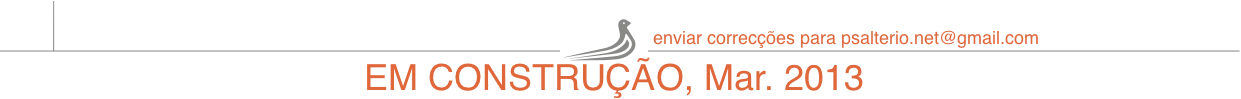
\includegraphics{_images/bkground_page_bottom.png}
}}





% this includes all the guitar tabs that may be needed
% must complete all the chords used in psalterio

% Cb chords

% C chords
\def \gtabCb{\gtab{Cb}{X32010:X32010}}
\def \gtabC{\gtab{C}{X32010:032010}}
\def \gtabCm{\gtab{Cm}{3:113321:004320}}

\def \gtabCsharpSusFour{\gtab{C\#sus4}{4:XX3341:XX2341}}

% Db chords

% D chords
\def \gtabD{\gtab{D}{X00232:000132}}
\def \gtabDm{\gtab{Dm}{X00231:000231}}
\def \gtabDfour{\gtab{D4}{X00233:000134}}
\def \gtabDseven{\gtab{D7}{X00212:000213}}
\def \gtabDsevenPlus{\gtab{D7+}{X00222:000111}}

% D#/Eb chords
\def \gtabDsharp{\gtab{D\#}{2:XX0232:000132}}

% E chords
\def \gtabE{\gtab{E}{022100:023100}}
\def \gtabEseven{\gtab{E}{020100:020100}}

\def \gtabEm{\gtab{Em}{022000:012000}}
\def \gtabEmSeven{\gtab{Em7}{022030:012040}}

% Gb chords

% F chords
\def \gtabF{\gtab{F}{1:133211:034200}}
\def \gtabFm{\gtab{Fm}{1:133111:034000}}


% F# chords
\def \gtabFsharpMinor{\gtab{F\#m}{2:133111:034000}}
\def \gtabFsharpMinorSeven{\gtab{F\#m7}{2:131131:030040}}

% Gb chords

% G chords
\def \gtabG{\gtab{G}{320033:210034}}
\def \gtabGseven{\gtab{G7}{320001:320001}}
\def \gtabGfret{\gtab{(G)}{3:133211:034200}}
\def \gtabGm{\gtab{Gm}{3:133111:034000}}


% G# / Ab chords

% A chords
\def \gtabA{\gtab{A}{X02220:001230}}
\def \gtabAm{\gtab{Am}{X02210:002310}}
\def \gtabAmSeven{\gtab{Am7}{X02010:002010}}
\def \gtabAfour{\gtab{A4}{X02230:001230}}
\def \gtabAseven{\gtab{A7}{X02020:001030}}

% Bb chords
\def \gtabBb{\gtab{Bb}{X13331}}

% B chords
\def \gtabB{\gtab{B}{X13331:003210}}
\def \gtabBm{\gtab{Bm}{X13321:003420}}
\def \gtabBmSeven{\gtab{Bm7}{X13121:003020}}



% after any { or } at the end of a line inside the macro definition add %, otherwise you'll get an extra space
\newcommand{\guitarTab}[1]{%
\ifstrequal{#1}{Cb}      {\gtab{Cb}{X32010:X32010}      }{}%
\ifstrequal{#1}{C}        { \gtab{C}{X32010:032010}       }{}%
%
%G
%
\ifstrequal{#1}{G}       { \gtab{G}{320033:210034}       }{}%
\ifstrequal{#1}{G7}     { \gtab{G7}{320001:320001}     }{}%
\ifstrequal{#1}{Gfret}  { \gtab{G}{3:133211:034200}    }{}%
\ifstrequal{#1}{Gm}    { \gtab{Gm}{3:133111:034000}  }{}%
} %end \newcommand{\gtab}

%muda aqui o numero da musica em que estas a trabalhar
%\def \selectSong{114}

\providebool{gchords}
\setbool{gchords}{true}

% set guitar chords vertical space separation with lyrics
\def \gchordsVspace{5 mm}

\begin{document}
	
	
	\AddToShipoutPicture*{\BottomPic}
	
	\begin{songs}{}
	
	%format file
	%
%Font Sizes
%
%\tiny
%\scriptsize
%\footnotesize
%\small
%\normalsize
%\large
%\Large
%\LARGE
%\huge
%\Huge


%\renewcommand{\thesongnum}{A\arabic{songnum}}
\renewcommand{\printsongnum}[1]{\sffamily\bfseries\huge\MakeUppercase#1}
\setlength{\songnumwidth}{2cm} % box width
%\renewcommand{\snumbgcolor}{white}

%change font for Title
\renewcommand{\stitlefont}{\sffamily\bfseries\huge\MakeUppercase} %song title

%remove verse numbers
%\noversenumbers 
% make left separation
\setlength{\versenumwidth}{2.0cm}

%verse separations
%\versesep=15pt
%\afterpreludeskip=2pt
%\beforepostludeskip=2pt
%\baselineadj=10pt

% separation between chords and lyrics
\renewcommand{\clineparams}{ 
\baselineskip=10pt 
%\lineskiplimit=2pt 
%\lineskip=5pt
}

% change font for lyrics
%\renewcommand{\lyricfont}{\sffamily}
%\renewcommand{\lyricfont}{\sffamily\small}
\renewcommand{\lyricfont}{\sffamily\large}
%\renewcommand{\chorusfont}{\sffamily}
\renewcommand{\chorusfont}{\sffamily\large}

%change the Chords formatting
\renewcommand{\printchord}[1]{\sffamily\color{red}\it\normalsize#1}

%check http://www.tug.org/pracjourn/2006-1/schmidt/schmidt.pdf


%\renewcommand{\songauthors}[1]{tete #1}


%\renewcommand{\extendpostlude}
%{ \songcopyright\ \songlicense\unskip \ Used with permission.}

\setlength{\cbarwidth}{0pt}
\setlength{\sbarheight}{0pt}

% music anf lyrics by
\newcommand{\musicLyricsBy}{} 
\newsongkey{mlby}{\def\musicLyricsBy{}}
                 {\def\musicLyricsBy{\sffamily\it\small letra e música por #1\par}}

% music anf lyrics by
\newcommand{\musicby}{} 
\newsongkey{music}{\def\musicby{}}
                 {\def\musicby{\sffamily\it\small música: #1\par}}

% music anf lyrics by
\newcommand{\lyricsby}{} 
\newsongkey{lyrics}{\def\lyricsby{}}
                 {\def\lyricsby{\sffamily\it\small letra: #1\par}}

%\renewcommand{\sharpsymbol}{\ensuremath{^\sharp}}
\renewcommand{\extendprelude}{
  \showrefs\showauthors 
  %{\bfseries\musicLyricsBy}
  {\bfseries\musicby}
  {\bfseries\lyricsby}
}

\def \gtabsOn{1}
	

%%%%%%%%%%%%%%%%%%%%%%%%%%%%%%%%%%%%%%%%%%%%%%%%%%%%%%%%%%%%%%%%%%%%%%%%%%%
% set song number
%%%%%%%%%%%%%%%%%%%%%%%%%%%%%%%%%%%%%%%%%%%%%%%%%%%%%%%%%%%%%%%%%%%%%%%%%%%
\setcounter{songnum}{9}

%%%%%%%%%%%%%%%%%%%%%%%%%%%%%%%%%%%%%%%%%%%%%%%%%%%%%%%%%%%%%%%%%%%%%%%%%%%
% begin song latex formating, set the title and other info
%%%%%%%%%%%%%%%%%%%%%%%%%%%%%%%%%%%%%%%%%%%%%%%%%%%%%%%%%%%%%%%%%%%%%%%%%%%
% song title
\beginsong{Old time religion}[
% music and lyric by
mlby={},
% lyrics
%lyrics={},
% music by
%music={},
% bible verse
%sr={},
% licence/copyright
%cr={Public domain.},
% arrangement by
%arr={},
% index title
index={Old time religion}]

%%%%%%%%%%%%%%%%%%%%%%%%%%%%%%%%%%%%%%%%%%%%%%%%%%%%%%%%%%%%%%%%%%%%%%%%%%%
% section #1: verse 
%%%%%%%%%%%%%%%%%%%%%%%%%%%%%%%%%%%%%%%%%%%%%%%%%%%%%%%%%%%%%%%%%%%%%%%%%%%
\beginverse
It’s the \[G]old time religion,
It’s the \[D]old time \[G]religion,
It’s the old time \[C]religion
And it’s \[G]good en\[D]ough for \[G]me.
\endverse

%%%%%%%%%%%%%%%%%%%%%%%%%%%%%%%%%%%%%%%%%%%%%%%%%%%%%%%%%%%%%%%%%%%%%%%%%%%
% section #2: verse 
%%%%%%%%%%%%%%%%%%%%%%%%%%%%%%%%%%%%%%%%%%%%%%%%%%%%%%%%%%%%%%%%%%%%%%%%%%%
\beginverse
\chordsoff
It was good for Paul and Silas, (3x)
And it’s good enough for me.
\endverse

%%%%%%%%%%%%%%%%%%%%%%%%%%%%%%%%%%%%%%%%%%%%%%%%%%%%%%%%%%%%%%%%%%%%%%%%%%%
% section #3: verse 
%%%%%%%%%%%%%%%%%%%%%%%%%%%%%%%%%%%%%%%%%%%%%%%%%%%%%%%%%%%%%%%%%%%%%%%%%%%
\beginverse
\chordsoff
It was good for our fathers,
It was good for our mothers,
It was good for our parents,
And it’s good enough for me.
\endverse

%%%%%%%%%%%%%%%%%%%%%%%%%%%%%%%%%%%%%%%%%%%%%%%%%%%%%%%%%%%%%%%%%%%%%%%%%%%
% section #4: verse 
%%%%%%%%%%%%%%%%%%%%%%%%%%%%%%%%%%%%%%%%%%%%%%%%%%%%%%%%%%%%%%%%%%%%%%%%%%%
\beginverse
\chordsoff
It is good for my brother,
It is good for my neighbor,
It is good for my country,
And it’s good enough for me.
\endverse

%%%%%%%%%%%%%%%%%%%%%%%%%%%%%%%%%%%%%%%%%%%%%%%%%%%%%%%%%%%%%%%%%%%%%%%%%%%
% section #5: verse 
%%%%%%%%%%%%%%%%%%%%%%%%%%%%%%%%%%%%%%%%%%%%%%%%%%%%%%%%%%%%%%%%%%%%%%%%%%%
\beginverse
\chordsoff
Makes me love ev’rybody, (3x)
And is good enough for me.
\endverse

%%%%%%%%%%%%%%%%%%%%%%%%%%%%%%%%%%%%%%%%%%%%%%%%%%%%%%%%%%%%%%%%%%%%%%%%%%%
% print guitar tabs used in this song
%%%%%%%%%%%%%%%%%%%%%%%%%%%%%%%%%%%%%%%%%%%%%%%%%%%%%%%%%%%%%%%%%%%%%%%%%%%
% if the guitar chords are to be printed
\ifbool{gchords}{
% set a vertical space of 10 pt 
\vspace{\gchordsVspace}
} % end if

%%%%%%%%%%%%%%%%%%%%%%%%%%%%%%%%%%%%%%%%%%%%%%%%%%%%%%%%%%%%%%%%%%%%%%%%%%%
% end song latex formating
%%%%%%%%%%%%%%%%%%%%%%%%%%%%%%%%%%%%%%%%%%%%%%%%%%%%%%%%%%%%%%%%%%%%%%%%%%%
% end song
\endsong

%include song latex footer
%	 %lilypond-book --output=out --pdf  106single.tex
	 %\lilypondfile[]{E_101.ly}
	
\end{document}
	%%%%%%%%%%%%%%%%%%%%%%%%%%%%%%%%%%%%%%%%%%%%%%%%%%%%%%%%%%%%%%%%%%%%%%%%%%%
% set song number
%%%%%%%%%%%%%%%%%%%%%%%%%%%%%%%%%%%%%%%%%%%%%%%%%%%%%%%%%%%%%%%%%%%%%%%%%%%
\setcounter{songnum}{10}
%%%%%%%%%%%%%%%%%%%%%%%%%%%%%%%%%%%%%%%%%%%%%%%%%%%%%%%%%%%%%%%%%%%%%%%%%%%
% begin song latex formating, set the title and other info
%%%%%%%%%%%%%%%%%%%%%%%%%%%%%%%%%%%%%%%%%%%%%%%%%%%%%%%%%%%%%%%%%%%%%%%%%%%
\beginsong{Vencendo Vem Jesus}[            % song title ...
%mlby={},                           % music and lyric by
%sr={Revelation 5:13},        % bible verse
%cr={Public domain.},         % licence
%arr={my},                          % arrangement by
index={Vencendo Vem Jesus}]               % index title ...	

%%%%%%%%%%%%%%%%%%%%%%%%%%%%%%%%%%%%%%%%%%%%%%%%%%%%%%%%%%%%%%%%%%%%%%%%%%%
% verse #1
%%%%%%%%%%%%%%%%%%%%%%%%%%%%%%%%%%%%%%%%%%%%%%%%%%%%%%%%%%%%%%%%%%%%%%%%%%%
\beginverse                       % start verse
\[C]Já refulge a glória eterna 
de Je\[C7+]sus, o Rei dos reis.
Breve os \[F]reinos deste mundo 
ouv\[C]irão as suas leis!
Os sinais da Sua vinda 
Mais se mostra\[C7+]m cad\[Am]a vez.
Venc\[Dm]endo \[C]vem \[G7]Jes\[C]us!
\endverse                         % end verse

%%%%%%%%%%%%%%%%%%%%%%%%%%%%%%%%%%%%%%%%%%%%%%%%%%%%%%%%%%%%%%%%%%%%%%%%%%%
% verse #2
%%%%%%%%%%%%%%%%%%%%%%%%%%%%%%%%%%%%%%%%%%%%%%%%%%%%%%%%%%%%%%%%%%%%%%%%%%%
\beginverse                       % start verse
\[C]Glória, glória! aleluia! \[F]glória, glória! al\[C]eluia!                           
Glória, glória! ale\[Am]luia! Venc\[Dm]endo \[C]vem \[G7]Jes\[C]us!
\endverse                         % start verse

%%%%%%%%%%%%%%%%%%%%%%%%%%%%%%%%%%%%%%%%%%%%%%%%%%%%%%%%%%%%%%%%%%%%%%%%%%%
% verse #3
%%%%%%%%%%%%%%%%%%%%%%%%%%%%%%%%%%%%%%%%%%%%%%%%%%%%%%%%%%%%%%%%%%%%%%%%%%%
\beginverse                       % start verse
\[C]O clarim que chama aos crentes à ba\[C7+]talha, já soou;
Cristo, à \[F]frente do seu povo, mul\[C]tidões já conquistou.
O inimigo, em retirada, seu furor pa\[C7+]tente\[Am]ou.
Venc\[Dm]endo \[C]vem \[G7]Jes\[C]us!
\endverse                         % start verse

%%%%%%%%%%%%%%%%%%%%%%%%%%%%%%%%%%%%%%%%%%%%%%%%%%%%%%%%%%%%%%%%%%%%%%%%%%%
% verse #4
%%%%%%%%%%%%%%%%%%%%%%%%%%%%%%%%%%%%%%%%%%%%%%%%%%%%%%%%%%%%%%%%%%%%%%%%%%%
\beginverse                       % start verse
\[C]E por fim entronizado as na\[C7+]ões há-de julgar,
Todos, \[F]grandes e pequenos, O \[C]Juiz hão-de encarar.
E os remidos triunfantes, em fulgor\[C7+] hão-de can\[Am]tar.
Venc\[Dm]endo \[C]vem \[G7]Jes\[C]us!
\endverse                         % start verse

%%%%%%%%%%%%%%%%%%%%%%%%%%%%%%%%%%%%%%%%%%%%%%%%%%%%%%%%%%%%%%%%%%%%%%%%%%%
% print guitar tabs used in this song
%%%%%%%%%%%%%%%%%%%%%%%%%%%%%%%%%%%%%%%%%%%%%%%%%%%%%%%%%%%%%%%%%%%%%%%%%%%
\ifbool{gchords}{                 % if the guitar chords are to be printed
\vspace{\gchordsVspace}           % set a vertical space of 10 pt 
\gtabC
\gtabF
%\gtabGseven
\gtabFsharpMinor
\gtabBm
}                                 % end if

%%%%%%%%%%%%%%%%%%%%%%%%%%%%%%%%%%%%%%%%%%%%%%%%%%%%%%%%%%%%%%%%%%%%%%%%%%%
% end song latex formating
%%%%%%%%%%%%%%%%%%%%%%%%%%%%%%%%%%%%%%%%%%%%%%%%%%%%%%%%%%%%%%%%%%%%%%%%%%%
\endsong                          % end song
%	 %lilypond-book --output=out --pdf  106single.tex
	 %\lilypondfile[]{E_101.ly}
	
\end{document}
	% percentagem é comentário
% 1 - \setcounter{songnum}{0} - numero da musica
% 2 - \beginsong{Pescadores de Homens}[ - título da música
% 3 -  index={Pescadores de Homens}] - entrada do indice da musica
% 4 - \beginverse , depois desta linha adicionar a letra
%%%%%%%%%%%%%%%%%%%%%%%%%%%%%%%%%%%%%%%%%%%%%%%%%%%%%%%%%%%%%%%%%%%%%%%%%%%
% this has all the necessary packages and formatting for the document
%%%%%%%%%%%%%%%%%%%%%%%%%%%%%%%%%%%%%%%%%%%%%%%%%%%%%%%%%%%%%%%%%%%%%%%%%%%
%\def \includeFolder{../_include}

% this has all the necessary packages and formatting for the document
\documentclass[10pt,a5paper]{article}

%define include folder
\def \includeFolder{_include}

%packages
\usepackage[left=1cm,right=1cm,top=1cm,bottom=1cm]{geometry}

\usepackage[chorded]{\includeFolder/psalterio} %must check the licence to change the name of the sty file!!!
%\usepackage[chorded]{resources/songs-old} %must check the licence to change the name of the sty file!!!

\usepackage[utf8]{inputenc}

\usepackage{graphicx}
\usepackage{wrapfig}
\usepackage{wallpaper}
\usepackage{color}
\usepackage{eso-pic} %for background pictures
\usepackage[bookmarks]{hyperref} 
%\usepackage{ifthen} %etoolbox is more up to date
\usepackage{etoolbox}


%\usepackage[xetex]{graphicx}
%\usepackage{fontspec,xunicode}
%\defaultfontfeatures{Mapping=tex-text,Scale=MatchLowercase}
%\setmainfont[Scale=.95]{Times}
%\setmonofont{Lucida Sans Typewriter}

%\usepackage[portuguese]{babel}
%\usepackage[latin1]{inputenc}
%\usepackage[utf8]{inputenc}
%\usepackage[T1]{fontenc}
%\usepackage[scaled]{uarial}
%\usepackage{helvet}
%\renewcommand{\familydefault}{\sfdefault}

%this removes the page number
\thispagestyle{empty}
\pagestyle{empty}
\songcolumns{1}

\parindent 0pt

%add background picture
\newcommand\BackgroundPic{
\put(0,0){
\parbox[b][\paperheight]{\paperwidth}{%
\vfill
\centering

\includegraphics[width=\paperwidth,height=\paperheight,
keepaspectratio]{logo.png}%
\vfill
}}}

\newcommand\BottomPic{
\put(0,0){
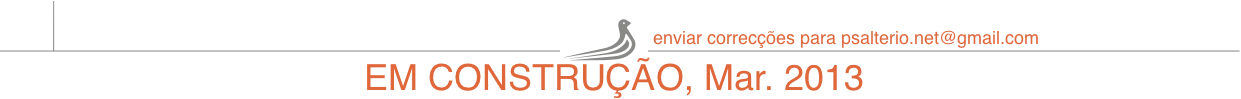
\includegraphics{_images/bkground_page_bottom.png}
}}





% this includes all the guitar tabs that may be needed
% must complete all the chords used in psalterio

% Cb chords

% C chords
\def \gtabCb{\gtab{Cb}{X32010:X32010}}
\def \gtabC{\gtab{C}{X32010:032010}}
\def \gtabCm{\gtab{Cm}{3:113321:004320}}

\def \gtabCsharpSusFour{\gtab{C\#sus4}{4:XX3341:XX2341}}

% Db chords

% D chords
\def \gtabD{\gtab{D}{X00232:000132}}
\def \gtabDm{\gtab{Dm}{X00231:000231}}
\def \gtabDfour{\gtab{D4}{X00233:000134}}
\def \gtabDseven{\gtab{D7}{X00212:000213}}
\def \gtabDsevenPlus{\gtab{D7+}{X00222:000111}}

% D#/Eb chords
\def \gtabDsharp{\gtab{D\#}{2:XX0232:000132}}

% E chords
\def \gtabE{\gtab{E}{022100:023100}}
\def \gtabEseven{\gtab{E}{020100:020100}}

\def \gtabEm{\gtab{Em}{022000:012000}}
\def \gtabEmSeven{\gtab{Em7}{022030:012040}}

% Gb chords

% F chords
\def \gtabF{\gtab{F}{1:133211:034200}}
\def \gtabFm{\gtab{Fm}{1:133111:034000}}


% F# chords
\def \gtabFsharpMinor{\gtab{F\#m}{2:133111:034000}}
\def \gtabFsharpMinorSeven{\gtab{F\#m7}{2:131131:030040}}

% Gb chords

% G chords
\def \gtabG{\gtab{G}{320033:210034}}
\def \gtabGseven{\gtab{G7}{320001:320001}}
\def \gtabGfret{\gtab{(G)}{3:133211:034200}}
\def \gtabGm{\gtab{Gm}{3:133111:034000}}


% G# / Ab chords

% A chords
\def \gtabA{\gtab{A}{X02220:001230}}
\def \gtabAm{\gtab{Am}{X02210:002310}}
\def \gtabAmSeven{\gtab{Am7}{X02010:002010}}
\def \gtabAfour{\gtab{A4}{X02230:001230}}
\def \gtabAseven{\gtab{A7}{X02020:001030}}

% Bb chords
\def \gtabBb{\gtab{Bb}{X13331}}

% B chords
\def \gtabB{\gtab{B}{X13331:003210}}
\def \gtabBm{\gtab{Bm}{X13321:003420}}
\def \gtabBmSeven{\gtab{Bm7}{X13121:003020}}



% after any { or } at the end of a line inside the macro definition add %, otherwise you'll get an extra space
\newcommand{\guitarTab}[1]{%
\ifstrequal{#1}{Cb}      {\gtab{Cb}{X32010:X32010}      }{}%
\ifstrequal{#1}{C}        { \gtab{C}{X32010:032010}       }{}%
%
%G
%
\ifstrequal{#1}{G}       { \gtab{G}{320033:210034}       }{}%
\ifstrequal{#1}{G7}     { \gtab{G7}{320001:320001}     }{}%
\ifstrequal{#1}{Gfret}  { \gtab{G}{3:133211:034200}    }{}%
\ifstrequal{#1}{Gm}    { \gtab{Gm}{3:133111:034000}  }{}%
} %end \newcommand{\gtab}

%muda aqui o numero da musica em que estas a trabalhar
%\def \selectSong{114}

\providebool{gchords}
\setbool{gchords}{true}

% set guitar chords vertical space separation with lyrics
\def \gchordsVspace{5 mm}

\begin{document}
	
	
	\AddToShipoutPicture*{\BottomPic}
	
	\begin{songs}{}
	
	%format file
	%
%Font Sizes
%
%\tiny
%\scriptsize
%\footnotesize
%\small
%\normalsize
%\large
%\Large
%\LARGE
%\huge
%\Huge


%\renewcommand{\thesongnum}{A\arabic{songnum}}
\renewcommand{\printsongnum}[1]{\sffamily\bfseries\huge\MakeUppercase#1}
\setlength{\songnumwidth}{2cm} % box width
%\renewcommand{\snumbgcolor}{white}

%change font for Title
\renewcommand{\stitlefont}{\sffamily\bfseries\huge\MakeUppercase} %song title

%remove verse numbers
%\noversenumbers 
% make left separation
\setlength{\versenumwidth}{2.0cm}

%verse separations
%\versesep=15pt
%\afterpreludeskip=2pt
%\beforepostludeskip=2pt
%\baselineadj=10pt

% separation between chords and lyrics
\renewcommand{\clineparams}{ 
\baselineskip=10pt 
%\lineskiplimit=2pt 
%\lineskip=5pt
}

% change font for lyrics
%\renewcommand{\lyricfont}{\sffamily}
%\renewcommand{\lyricfont}{\sffamily\small}
\renewcommand{\lyricfont}{\sffamily\large}
%\renewcommand{\chorusfont}{\sffamily}
\renewcommand{\chorusfont}{\sffamily\large}

%change the Chords formatting
\renewcommand{\printchord}[1]{\sffamily\color{red}\it\normalsize#1}

%check http://www.tug.org/pracjourn/2006-1/schmidt/schmidt.pdf


%\renewcommand{\songauthors}[1]{tete #1}


%\renewcommand{\extendpostlude}
%{ \songcopyright\ \songlicense\unskip \ Used with permission.}

\setlength{\cbarwidth}{0pt}
\setlength{\sbarheight}{0pt}

% music anf lyrics by
\newcommand{\musicLyricsBy}{} 
\newsongkey{mlby}{\def\musicLyricsBy{}}
                 {\def\musicLyricsBy{\sffamily\it\small letra e música por #1\par}}

% music anf lyrics by
\newcommand{\musicby}{} 
\newsongkey{music}{\def\musicby{}}
                 {\def\musicby{\sffamily\it\small música: #1\par}}

% music anf lyrics by
\newcommand{\lyricsby}{} 
\newsongkey{lyrics}{\def\lyricsby{}}
                 {\def\lyricsby{\sffamily\it\small letra: #1\par}}

%\renewcommand{\sharpsymbol}{\ensuremath{^\sharp}}
\renewcommand{\extendprelude}{
  \showrefs\showauthors 
  %{\bfseries\musicLyricsBy}
  {\bfseries\musicby}
  {\bfseries\lyricsby}
}

\def \gtabsOn{1}
	

%%%%%%%%%%%%%%%%%%%%%%%%%%%%%%%%%%%%%%%%%%%%%%%%%%%%%%%%%%%%%%%%%%%%%%%%%%%
% set song number
%%%%%%%%%%%%%%%%%%%%%%%%%%%%%%%%%%%%%%%%%%%%%%%%%%%%%%%%%%%%%%%%%%%%%%%%%%%
\setcounter{songnum}{11}       % song number

%%%%%%%%%%%%%%%%%%%%%%%%%%%%%%%%%%%%%%%%%%%%%%%%%%%%%%%%%%%%%%%%%%%%%%%%%%%
% begin song latex formating, set the title and other info
%%%%%%%%%%%%%%%%%%%%%%%%%%%%%%%%%%%%%%%%%%%%%%%%%%%%%%%%%%%%%%%%%%%%%%%%%%%
\beginsong{Pescadores de Homens}[            % song title ...
    %mlby={},                           % music and lyric by
    %sr={Revelation 5:13},        % bible verse
    %cr={Public domain.},         % licence
    %arr={my},                          % arrangement by
    index={Pescadores de Homens}]               % index title ...	

%%%%%%%%%%%%%%%%%%%%%%%%%%%%%%%%%%%%%%%%%%%%%%%%%%%%%%%%%%%%%%%%%%%%%%%%%%%
% verse #1
%%%%%%%%%%%%%%%%%%%%%%%%%%%%%%%%%%%%%%%%%%%%%%%%%%%%%%%%%%%%%%%%%%%%%%%%%%%
\beginverse                       % start verse

\[F]Pescadores de homens sereis,
  
De \[C7]homens sereis, d\[Bb]e homens\[F] sereis;
                                                
Pescadores de homens sereis,\[C7] s\[F]eguind\[C7]o a \[F]Mim
                
Seguindo a \[F5-F]Mim, se\[Bb]guindo a \[F]Mim,
                                                 
Pescadores de homens sereis,\[C7] s\[F]eguind\[C7]o a \[F]Mim.

\endverse                         % end verse

%%%%%%%%%%%%%%%%%%%%%%%%%%%%%%%%%%%%%%%%%%%%%%%%%%%%%%%%%%%%%%%%%%%%%%%%%%%
% verse #2
%%%%%%%%%%%%%%%%%%%%%%%%%%%%%%%%%%%%%%%%%%%%%%%%%%%%%%%%%%%%%%%%%%%%%%%%%%%
\beginverse                       % start verse

\[F]Muitas almas tu ganharas,

Tu \[C7]ganharas, tu\[Bb] ga\[F]nharas;

Muitas almas tu ganharas, \[C7] s\[F]eguind\[C7]o a \[F]Mim

Seguindo a \[F5-F]Mim, se\[Bb]guindo a \[F]Mim,

 Muitas almas tu ganharas, \[C7] s\[F]eguind\[C7]o a \[F]Mim.


\endverse                         % start verse

%%%%%%%%%%%%%%%%%%%%%%%%%%%%%%%%%%%%%%%%%%%%%%%%%%%%%%%%%%%%%%%%%%%%%%%%%%%
% verse #3
%%%%%%%%%%%%%%%%%%%%%%%%%%%%%%%%%%%%%%%%%%%%%%%%%%%%%%%%%%%%%%%%%%%%%%%%%%%
\beginverse                       % start verse

\[F]Galardao tu receberas,

Re\[C7]ceberas, re\[Bb]cebe\[F]ras;

Galardao tu receberas, \[C7] s\[F]eguind\[C7]o a \[F]Mim
 
Seguindo a \[F5-F]Mim, se\[Bb]guindo a \[F]Mim,

Galardao tu receberas, \[C7] s\[F]eguind\[C7]o a \[F]Mim.


\endverse                         % start verse

%%%%%%%%%%%%%%%%%%%%%%%%%%%%%%%%%%%%%%%%%%%%%%%%%%%%%%%%%%%%%%%%%%%%%%%%%%%
% print guitar tabs used in this song
%%%%%%%%%%%%%%%%%%%%%%%%%%%%%%%%%%%%%%%%%%%%%%%%%%%%%%%%%%%%%%%%%%%%%%%%%%%
\ifbool{gchords}{                 % if the guitar chords are to be printed
\vspace{\gchordsVspace}           % set a vertical space of 10 pt 

\gtabC
\gtabF
%\gtabGseven
\gtabFsharpMinor
\gtabBm

}                                 % end if

%%%%%%%%%%%%%%%%%%%%%%%%%%%%%%%%%%%%%%%%%%%%%%%%%%%%%%%%%%%%%%%%%%%%%%%%%%%
% end song latex formating
%%%%%%%%%%%%%%%%%%%%%%%%%%%%%%%%%%%%%%%%%%%%%%%%%%%%%%%%%%%%%%%%%%%%%%%%%%%
\endsong                          % end song
%	 %lilypond-book --output=out --pdf  106single.tex
	 %\lilypondfile[]{E_101.ly}
	
\end{document}
	%%%%%%%%%%%%%%%%%%%%%%%%%%%%%%%%%%%%%%%%%%%%%%%%%%%%%%%%%%%%%%%%%%%%%%%%%%%
% this has all the necessary packages and formatting for the document
%%%%%%%%%%%%%%%%%%%%%%%%%%%%%%%%%%%%%%%%%%%%%%%%%%%%%%%%%%%%%%%%%%%%%%%%%%%
%\def \includeFolder{../_include}

% this has all the necessary packages and formatting for the document
\documentclass[10pt,a5paper]{article}

%define include folder
\def \includeFolder{_include}

%packages
\usepackage[left=1cm,right=1cm,top=1cm,bottom=1cm]{geometry}

\usepackage[chorded]{\includeFolder/psalterio} %must check the licence to change the name of the sty file!!!
%\usepackage[chorded]{resources/songs-old} %must check the licence to change the name of the sty file!!!

\usepackage[utf8]{inputenc}

\usepackage{graphicx}
\usepackage{wrapfig}
\usepackage{wallpaper}
\usepackage{color}
\usepackage{eso-pic} %for background pictures
\usepackage[bookmarks]{hyperref} 
%\usepackage{ifthen} %etoolbox is more up to date
\usepackage{etoolbox}


%\usepackage[xetex]{graphicx}
%\usepackage{fontspec,xunicode}
%\defaultfontfeatures{Mapping=tex-text,Scale=MatchLowercase}
%\setmainfont[Scale=.95]{Times}
%\setmonofont{Lucida Sans Typewriter}

%\usepackage[portuguese]{babel}
%\usepackage[latin1]{inputenc}
%\usepackage[utf8]{inputenc}
%\usepackage[T1]{fontenc}
%\usepackage[scaled]{uarial}
%\usepackage{helvet}
%\renewcommand{\familydefault}{\sfdefault}

%this removes the page number
\thispagestyle{empty}
\pagestyle{empty}
\songcolumns{1}

\parindent 0pt

%add background picture
\newcommand\BackgroundPic{
\put(0,0){
\parbox[b][\paperheight]{\paperwidth}{%
\vfill
\centering

\includegraphics[width=\paperwidth,height=\paperheight,
keepaspectratio]{logo.png}%
\vfill
}}}

\newcommand\BottomPic{
\put(0,0){
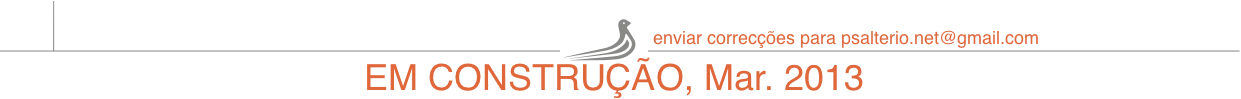
\includegraphics{_images/bkground_page_bottom.png}
}}





% this includes all the guitar tabs that may be needed
% must complete all the chords used in psalterio

% Cb chords

% C chords
\def \gtabCb{\gtab{Cb}{X32010:X32010}}
\def \gtabC{\gtab{C}{X32010:032010}}
\def \gtabCm{\gtab{Cm}{3:113321:004320}}

\def \gtabCsharpSusFour{\gtab{C\#sus4}{4:XX3341:XX2341}}

% Db chords

% D chords
\def \gtabD{\gtab{D}{X00232:000132}}
\def \gtabDm{\gtab{Dm}{X00231:000231}}
\def \gtabDfour{\gtab{D4}{X00233:000134}}
\def \gtabDseven{\gtab{D7}{X00212:000213}}
\def \gtabDsevenPlus{\gtab{D7+}{X00222:000111}}

% D#/Eb chords
\def \gtabDsharp{\gtab{D\#}{2:XX0232:000132}}

% E chords
\def \gtabE{\gtab{E}{022100:023100}}
\def \gtabEseven{\gtab{E}{020100:020100}}

\def \gtabEm{\gtab{Em}{022000:012000}}
\def \gtabEmSeven{\gtab{Em7}{022030:012040}}

% Gb chords

% F chords
\def \gtabF{\gtab{F}{1:133211:034200}}
\def \gtabFm{\gtab{Fm}{1:133111:034000}}


% F# chords
\def \gtabFsharpMinor{\gtab{F\#m}{2:133111:034000}}
\def \gtabFsharpMinorSeven{\gtab{F\#m7}{2:131131:030040}}

% Gb chords

% G chords
\def \gtabG{\gtab{G}{320033:210034}}
\def \gtabGseven{\gtab{G7}{320001:320001}}
\def \gtabGfret{\gtab{(G)}{3:133211:034200}}
\def \gtabGm{\gtab{Gm}{3:133111:034000}}


% G# / Ab chords

% A chords
\def \gtabA{\gtab{A}{X02220:001230}}
\def \gtabAm{\gtab{Am}{X02210:002310}}
\def \gtabAmSeven{\gtab{Am7}{X02010:002010}}
\def \gtabAfour{\gtab{A4}{X02230:001230}}
\def \gtabAseven{\gtab{A7}{X02020:001030}}

% Bb chords
\def \gtabBb{\gtab{Bb}{X13331}}

% B chords
\def \gtabB{\gtab{B}{X13331:003210}}
\def \gtabBm{\gtab{Bm}{X13321:003420}}
\def \gtabBmSeven{\gtab{Bm7}{X13121:003020}}



% after any { or } at the end of a line inside the macro definition add %, otherwise you'll get an extra space
\newcommand{\guitarTab}[1]{%
\ifstrequal{#1}{Cb}      {\gtab{Cb}{X32010:X32010}      }{}%
\ifstrequal{#1}{C}        { \gtab{C}{X32010:032010}       }{}%
%
%G
%
\ifstrequal{#1}{G}       { \gtab{G}{320033:210034}       }{}%
\ifstrequal{#1}{G7}     { \gtab{G7}{320001:320001}     }{}%
\ifstrequal{#1}{Gfret}  { \gtab{G}{3:133211:034200}    }{}%
\ifstrequal{#1}{Gm}    { \gtab{Gm}{3:133111:034000}  }{}%
} %end \newcommand{\gtab}

%muda aqui o numero da musica em que estas a trabalhar
%\def \selectSong{114}

\providebool{gchords}
\setbool{gchords}{true}

% set guitar chords vertical space separation with lyrics
\def \gchordsVspace{5 mm}

\begin{document}
	
	
	\AddToShipoutPicture*{\BottomPic}
	
	\begin{songs}{}
	
	%format file
	%
%Font Sizes
%
%\tiny
%\scriptsize
%\footnotesize
%\small
%\normalsize
%\large
%\Large
%\LARGE
%\huge
%\Huge


%\renewcommand{\thesongnum}{A\arabic{songnum}}
\renewcommand{\printsongnum}[1]{\sffamily\bfseries\huge\MakeUppercase#1}
\setlength{\songnumwidth}{2cm} % box width
%\renewcommand{\snumbgcolor}{white}

%change font for Title
\renewcommand{\stitlefont}{\sffamily\bfseries\huge\MakeUppercase} %song title

%remove verse numbers
%\noversenumbers 
% make left separation
\setlength{\versenumwidth}{2.0cm}

%verse separations
%\versesep=15pt
%\afterpreludeskip=2pt
%\beforepostludeskip=2pt
%\baselineadj=10pt

% separation between chords and lyrics
\renewcommand{\clineparams}{ 
\baselineskip=10pt 
%\lineskiplimit=2pt 
%\lineskip=5pt
}

% change font for lyrics
%\renewcommand{\lyricfont}{\sffamily}
%\renewcommand{\lyricfont}{\sffamily\small}
\renewcommand{\lyricfont}{\sffamily\large}
%\renewcommand{\chorusfont}{\sffamily}
\renewcommand{\chorusfont}{\sffamily\large}

%change the Chords formatting
\renewcommand{\printchord}[1]{\sffamily\color{red}\it\normalsize#1}

%check http://www.tug.org/pracjourn/2006-1/schmidt/schmidt.pdf


%\renewcommand{\songauthors}[1]{tete #1}


%\renewcommand{\extendpostlude}
%{ \songcopyright\ \songlicense\unskip \ Used with permission.}

\setlength{\cbarwidth}{0pt}
\setlength{\sbarheight}{0pt}

% music anf lyrics by
\newcommand{\musicLyricsBy}{} 
\newsongkey{mlby}{\def\musicLyricsBy{}}
                 {\def\musicLyricsBy{\sffamily\it\small letra e música por #1\par}}

% music anf lyrics by
\newcommand{\musicby}{} 
\newsongkey{music}{\def\musicby{}}
                 {\def\musicby{\sffamily\it\small música: #1\par}}

% music anf lyrics by
\newcommand{\lyricsby}{} 
\newsongkey{lyrics}{\def\lyricsby{}}
                 {\def\lyricsby{\sffamily\it\small letra: #1\par}}

%\renewcommand{\sharpsymbol}{\ensuremath{^\sharp}}
\renewcommand{\extendprelude}{
  \showrefs\showauthors 
  %{\bfseries\musicLyricsBy}
  {\bfseries\musicby}
  {\bfseries\lyricsby}
}

\def \gtabsOn{1}
	

%%%%%%%%%%%%%%%%%%%%%%%%%%%%%%%%%%%%%%%%%%%%%%%%%%%%%%%%%%%%%%%%%%%%%%%%%%%
% set song number
%%%%%%%%%%%%%%%%%%%%%%%%%%%%%%%%%%%%%%%%%%%%%%%%%%%%%%%%%%%%%%%%%%%%%%%%%%%
\setcounter{songnum}{12}

%%%%%%%%%%%%%%%%%%%%%%%%%%%%%%%%%%%%%%%%%%%%%%%%%%%%%%%%%%%%%%%%%%%%%%%%%%%
% begin song latex formating, set the title and other info
%%%%%%%%%%%%%%%%%%%%%%%%%%%%%%%%%%%%%%%%%%%%%%%%%%%%%%%%%%%%%%%%%%%%%%%%%%%
% song title
\beginsong{Gozo no coração}[
        % music and lyric by
        % mlby={},
        % lyrics
        lyrics={}, 
        % music by
        music={},
        % bible verse
        %sr={},
        % licence/copyright
        %cr={Public domain.},
        % arrangement by
        %arr={},
        % index title
        index={Gozo no coração}]

%%%%%%%%%%%%%%%%%%%%%%%%%%%%%%%%%%%%%%%%%%%%%%%%%%%%%%%%%%%%%%%%%%%%%%%%%%%
% section #1: verse 
%%%%%%%%%%%%%%%%%%%%%%%%%%%%%%%%%%%%%%%%%%%%%%%%%%%%%%%%%%%%%%%%%%%%%%%%%%%
\beginverse
Eu tenho \[C]gozo, \[G7]gozo em \[C]meu \[G7]coração, \[G7]meu coração, \[C]meu coração,
Eu tenho gozo, gozo em meu coração, sempre em meu coração.
\endverse

%%%%%%%%%%%%%%%%%%%%%%%%%%%%%%%%%%%%%%%%%%%%%%%%%%%%%%%%%%%%%%%%%%%%%%%%%%%
% section #2: verse 
%%%%%%%%%%%%%%%%%%%%%%%%%%%%%%%%%%%%%%%%%%%%%%%%%%%%%%%%%%%%%%%%%%%%%%%%%%%
\beginverse
Eu tenho paz celeste em meu coração, meu coração, meu coração,
Eu tenho paz celeste em emu coração, sempre em meu coração.
\endverse

%%%%%%%%%%%%%%%%%%%%%%%%%%%%%%%%%%%%%%%%%%%%%%%%%%%%%%%%%%%%%%%%%%%%%%%%%%%
% section #3: verse 
%%%%%%%%%%%%%%%%%%%%%%%%%%%%%%%%%%%%%%%%%%%%%%%%%%%%%%%%%%%%%%%%%%%%%%%%%%%
\beginverse
Eu tenho a Cristo, Cristo em meu coração, meu coração, meu coração,
Eu tenho a Cristo, Cristo em meu coração, sempre em meu coração.
\endverse

%%%%%%%%%%%%%%%%%%%%%%%%%%%%%%%%%%%%%%%%%%%%%%%%%%%%%%%%%%%%%%%%%%%%%%%%%%%
% section #4: verse 
%%%%%%%%%%%%%%%%%%%%%%%%%%%%%%%%%%%%%%%%%%%%%%%%%%%%%%%%%%%%%%%%%%%%%%%%%%%
\beginverse
Eu tenho esperança em meu coração, meu coração, meu coração,
Eu tenho esperança em meu coração, sempre em meu coração
\endverse


%%%%%%%%%%%%%%%%%%%%%%%%%%%%%%%%%%%%%%%%%%%%%%%%%%%%%%%%%%%%%%%%%%%%%%%%%%%
% print guitar tabs used in this song
%%%%%%%%%%%%%%%%%%%%%%%%%%%%%%%%%%%%%%%%%%%%%%%%%%%%%%%%%%%%%%%%%%%%%%%%%%%
% if the guitar chords are to be printed
\ifbool{gchords}{
% set a vertical space of 10 pt 
\vspace{\gchordsVspace}
} % end if

%%%%%%%%%%%%%%%%%%%%%%%%%%%%%%%%%%%%%%%%%%%%%%%%%%%%%%%%%%%%%%%%%%%%%%%%%%%
% end song latex formating
%%%%%%%%%%%%%%%%%%%%%%%%%%%%%%%%%%%%%%%%%%%%%%%%%%%%%%%%%%%%%%%%%%%%%%%%%%%
% end song
\endsong

%include song latex footer
%	 %lilypond-book --output=out --pdf  106single.tex
	 %\lilypondfile[]{E_101.ly}
	
\end{document}
	%%%%%%%%%%%%%%%%%%%%%%%%%%%%%%%%%%%%%%%%%%%%%%%%%%%%%%%%%%%%%%%%%%%%%%%%%%%
% this has all the necessary packages and formatting for the document
%%%%%%%%%%%%%%%%%%%%%%%%%%%%%%%%%%%%%%%%%%%%%%%%%%%%%%%%%%%%%%%%%%%%%%%%%%%
%\def \includeFolder{../_include}

% this has all the necessary packages and formatting for the document
\documentclass[10pt,a5paper]{article}

%define include folder
\def \includeFolder{_include}

%packages
\usepackage[left=1cm,right=1cm,top=1cm,bottom=1cm]{geometry}

\usepackage[chorded]{\includeFolder/psalterio} %must check the licence to change the name of the sty file!!!
%\usepackage[chorded]{resources/songs-old} %must check the licence to change the name of the sty file!!!

\usepackage[utf8]{inputenc}

\usepackage{graphicx}
\usepackage{wrapfig}
\usepackage{wallpaper}
\usepackage{color}
\usepackage{eso-pic} %for background pictures
\usepackage[bookmarks]{hyperref} 
%\usepackage{ifthen} %etoolbox is more up to date
\usepackage{etoolbox}


%\usepackage[xetex]{graphicx}
%\usepackage{fontspec,xunicode}
%\defaultfontfeatures{Mapping=tex-text,Scale=MatchLowercase}
%\setmainfont[Scale=.95]{Times}
%\setmonofont{Lucida Sans Typewriter}

%\usepackage[portuguese]{babel}
%\usepackage[latin1]{inputenc}
%\usepackage[utf8]{inputenc}
%\usepackage[T1]{fontenc}
%\usepackage[scaled]{uarial}
%\usepackage{helvet}
%\renewcommand{\familydefault}{\sfdefault}

%this removes the page number
\thispagestyle{empty}
\pagestyle{empty}
\songcolumns{1}

\parindent 0pt

%add background picture
\newcommand\BackgroundPic{
\put(0,0){
\parbox[b][\paperheight]{\paperwidth}{%
\vfill
\centering

\includegraphics[width=\paperwidth,height=\paperheight,
keepaspectratio]{logo.png}%
\vfill
}}}

\newcommand\BottomPic{
\put(0,0){
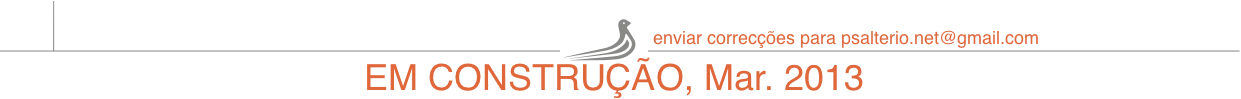
\includegraphics{_images/bkground_page_bottom.png}
}}





% this includes all the guitar tabs that may be needed
% must complete all the chords used in psalterio

% Cb chords

% C chords
\def \gtabCb{\gtab{Cb}{X32010:X32010}}
\def \gtabC{\gtab{C}{X32010:032010}}
\def \gtabCm{\gtab{Cm}{3:113321:004320}}

\def \gtabCsharpSusFour{\gtab{C\#sus4}{4:XX3341:XX2341}}

% Db chords

% D chords
\def \gtabD{\gtab{D}{X00232:000132}}
\def \gtabDm{\gtab{Dm}{X00231:000231}}
\def \gtabDfour{\gtab{D4}{X00233:000134}}
\def \gtabDseven{\gtab{D7}{X00212:000213}}
\def \gtabDsevenPlus{\gtab{D7+}{X00222:000111}}

% D#/Eb chords
\def \gtabDsharp{\gtab{D\#}{2:XX0232:000132}}

% E chords
\def \gtabE{\gtab{E}{022100:023100}}
\def \gtabEseven{\gtab{E}{020100:020100}}

\def \gtabEm{\gtab{Em}{022000:012000}}
\def \gtabEmSeven{\gtab{Em7}{022030:012040}}

% Gb chords

% F chords
\def \gtabF{\gtab{F}{1:133211:034200}}
\def \gtabFm{\gtab{Fm}{1:133111:034000}}


% F# chords
\def \gtabFsharpMinor{\gtab{F\#m}{2:133111:034000}}
\def \gtabFsharpMinorSeven{\gtab{F\#m7}{2:131131:030040}}

% Gb chords

% G chords
\def \gtabG{\gtab{G}{320033:210034}}
\def \gtabGseven{\gtab{G7}{320001:320001}}
\def \gtabGfret{\gtab{(G)}{3:133211:034200}}
\def \gtabGm{\gtab{Gm}{3:133111:034000}}


% G# / Ab chords

% A chords
\def \gtabA{\gtab{A}{X02220:001230}}
\def \gtabAm{\gtab{Am}{X02210:002310}}
\def \gtabAmSeven{\gtab{Am7}{X02010:002010}}
\def \gtabAfour{\gtab{A4}{X02230:001230}}
\def \gtabAseven{\gtab{A7}{X02020:001030}}

% Bb chords
\def \gtabBb{\gtab{Bb}{X13331}}

% B chords
\def \gtabB{\gtab{B}{X13331:003210}}
\def \gtabBm{\gtab{Bm}{X13321:003420}}
\def \gtabBmSeven{\gtab{Bm7}{X13121:003020}}



% after any { or } at the end of a line inside the macro definition add %, otherwise you'll get an extra space
\newcommand{\guitarTab}[1]{%
\ifstrequal{#1}{Cb}      {\gtab{Cb}{X32010:X32010}      }{}%
\ifstrequal{#1}{C}        { \gtab{C}{X32010:032010}       }{}%
%
%G
%
\ifstrequal{#1}{G}       { \gtab{G}{320033:210034}       }{}%
\ifstrequal{#1}{G7}     { \gtab{G7}{320001:320001}     }{}%
\ifstrequal{#1}{Gfret}  { \gtab{G}{3:133211:034200}    }{}%
\ifstrequal{#1}{Gm}    { \gtab{Gm}{3:133111:034000}  }{}%
} %end \newcommand{\gtab}

%muda aqui o numero da musica em que estas a trabalhar
%\def \selectSong{114}

\providebool{gchords}
\setbool{gchords}{true}

% set guitar chords vertical space separation with lyrics
\def \gchordsVspace{5 mm}

\begin{document}
	
	
	\AddToShipoutPicture*{\BottomPic}
	
	\begin{songs}{}
	
	%format file
	%
%Font Sizes
%
%\tiny
%\scriptsize
%\footnotesize
%\small
%\normalsize
%\large
%\Large
%\LARGE
%\huge
%\Huge


%\renewcommand{\thesongnum}{A\arabic{songnum}}
\renewcommand{\printsongnum}[1]{\sffamily\bfseries\huge\MakeUppercase#1}
\setlength{\songnumwidth}{2cm} % box width
%\renewcommand{\snumbgcolor}{white}

%change font for Title
\renewcommand{\stitlefont}{\sffamily\bfseries\huge\MakeUppercase} %song title

%remove verse numbers
%\noversenumbers 
% make left separation
\setlength{\versenumwidth}{2.0cm}

%verse separations
%\versesep=15pt
%\afterpreludeskip=2pt
%\beforepostludeskip=2pt
%\baselineadj=10pt

% separation between chords and lyrics
\renewcommand{\clineparams}{ 
\baselineskip=10pt 
%\lineskiplimit=2pt 
%\lineskip=5pt
}

% change font for lyrics
%\renewcommand{\lyricfont}{\sffamily}
%\renewcommand{\lyricfont}{\sffamily\small}
\renewcommand{\lyricfont}{\sffamily\large}
%\renewcommand{\chorusfont}{\sffamily}
\renewcommand{\chorusfont}{\sffamily\large}

%change the Chords formatting
\renewcommand{\printchord}[1]{\sffamily\color{red}\it\normalsize#1}

%check http://www.tug.org/pracjourn/2006-1/schmidt/schmidt.pdf


%\renewcommand{\songauthors}[1]{tete #1}


%\renewcommand{\extendpostlude}
%{ \songcopyright\ \songlicense\unskip \ Used with permission.}

\setlength{\cbarwidth}{0pt}
\setlength{\sbarheight}{0pt}

% music anf lyrics by
\newcommand{\musicLyricsBy}{} 
\newsongkey{mlby}{\def\musicLyricsBy{}}
                 {\def\musicLyricsBy{\sffamily\it\small letra e música por #1\par}}

% music anf lyrics by
\newcommand{\musicby}{} 
\newsongkey{music}{\def\musicby{}}
                 {\def\musicby{\sffamily\it\small música: #1\par}}

% music anf lyrics by
\newcommand{\lyricsby}{} 
\newsongkey{lyrics}{\def\lyricsby{}}
                 {\def\lyricsby{\sffamily\it\small letra: #1\par}}

%\renewcommand{\sharpsymbol}{\ensuremath{^\sharp}}
\renewcommand{\extendprelude}{
  \showrefs\showauthors 
  %{\bfseries\musicLyricsBy}
  {\bfseries\musicby}
  {\bfseries\lyricsby}
}

\def \gtabsOn{1}
	

%%%%%%%%%%%%%%%%%%%%%%%%%%%%%%%%%%%%%%%%%%%%%%%%%%%%%%%%%%%%%%%%%%%%%%%%%%%
% set song number
%%%%%%%%%%%%%%%%%%%%%%%%%%%%%%%%%%%%%%%%%%%%%%%%%%%%%%%%%%%%%%%%%%%%%%%%%%%
\setcounter{songnum}{13}

%%%%%%%%%%%%%%%%%%%%%%%%%%%%%%%%%%%%%%%%%%%%%%%%%%%%%%%%%%%%%%%%%%%%%%%%%%%
% begin song latex formating, set the title and other info
%%%%%%%%%%%%%%%%%%%%%%%%%%%%%%%%%%%%%%%%%%%%%%%%%%%%%%%%%%%%%%%%%%%%%%%%%%%
% song title
\beginsong{Oh! Prends Mon Âme}[
% music and lyric by
% mlby={},
% lyrics
%lyrics={}, 
% music by
%music={},
% bible verse
%sr={},
% licence/copyright
%cr={Public domain.},
% arrangement by
%arr={},
% index title
index={Oh! Prends Mon Âme}]

%%%%%%%%%%%%%%%%%%%%%%%%%%%%%%%%%%%%%%%%%%%%%%%%%%%%%%%%%%%%%%%%%%%%%%%%%%%
% section #1: verse 
%%%%%%%%%%%%%%%%%%%%%%%%%%%%%%%%%%%%%%%%%%%%%%%%%%%%%%%%%%%%%%%%%%%%%%%%%%%
\beginverse
\[Em]Oh! \[C]prends \[D7]mon \[G]âme, \[Am]prends-\[D7]la, Sei\[G]gneur,
\[Am]Et \[B7]que ta \[Em]flame \[B7]brûle en mon \[Em]coeur.
Que \[C]tout \[D7]mon \[G]être \[Am D7]vibre pour \[G]Toi,
\[Am]Sois \[B7]seul mon \[Em]Maître, \[B7]o divin \[Em]Roi.
\endverse

%%%%%%%%%%%%%%%%%%%%%%%%%%%%%%%%%%%%%%%%%%%%%%%%%%%%%%%%%%%%%%%%%%%%%%%%%%%
% section #2: chorus 
%%%%%%%%%%%%%%%%%%%%%%%%%%%%%%%%%%%%%%%%%%%%%%%%%%%%%%%%%%%%%%%%%%%%%%%%%%%
\beginchorus
Source de \[C]vie, \[D7]de paix d’a\[G]mour,
\[Em]Vers Toi je \[C]crie, \[D7]la nuit, le \[G]jour.
\[D#7dim]Entends \[Em]ma plainte, \[Am]sois mon sou\[G]tien,
\[D#7dmin B7]Calme ma crain\[Em]te, \[B7]Toi, mon seul \[Em]bien!
\endchorus

\chordsoff
%%%%%%%%%%%%%%%%%%%%%%%%%%%%%%%%%%%%%%%%%%%%%%%%%%%%%%%%%%%%%%%%%%%%%%%%%%%
% section #3: verse 
%%%%%%%%%%%%%%%%%%%%%%%%%%%%%%%%%%%%%%%%%%%%%%%%%%%%%%%%%%%%%%%%%%%%%%%%%%%
\beginverse
Du mal perfide, o garde-moi,
Viens, sois mon guide, chef de ma foi.
Quand la nuit voile tout à mes ywux,
Sois mon étoile, brille des cieux.
\endverse

%%%%%%%%%%%%%%%%%%%%%%%%%%%%%%%%%%%%%%%%%%%%%%%%%%%%%%%%%%%%%%%%%%%%%%%%%%%
% section #4: verse 
%%%%%%%%%%%%%%%%%%%%%%%%%%%%%%%%%%%%%%%%%%%%%%%%%%%%%%%%%%%%%%%%%%%%%%%%%%%
\beginverse
Voici l’aurore d’un jour nouveau,
Le ciel se dore de feux plus beaux.
Jésus s’apprête, pourquoi gémir?
Levons nos têtes, il va venir!
\endverse


%%%%%%%%%%%%%%%%%%%%%%%%%%%%%%%%%%%%%%%%%%%%%%%%%%%%%%%%%%%%%%%%%%%%%%%%%%%
% print guitar tabs used in this song
%%%%%%%%%%%%%%%%%%%%%%%%%%%%%%%%%%%%%%%%%%%%%%%%%%%%%%%%%%%%%%%%%%%%%%%%%%%
% if the guitar chords are to be printed
\ifbool{gchords}{
% set a vertical space of 10 pt 
\vspace{\gchordsVspace}
} % end if

%%%%%%%%%%%%%%%%%%%%%%%%%%%%%%%%%%%%%%%%%%%%%%%%%%%%%%%%%%%%%%%%%%%%%%%%%%%
% end song latex formating
%%%%%%%%%%%%%%%%%%%%%%%%%%%%%%%%%%%%%%%%%%%%%%%%%%%%%%%%%%%%%%%%%%%%%%%%%%%
% end song
\endsong

%include song latex footer
%	 %lilypond-book --output=out --pdf  106single.tex
	 %\lilypondfile[]{E_101.ly}
	
\end{document}
	\setcounter{songnum}{14}

\beginsong{Cum ba Yá}[
mlby={},
%sr={Revelation 5:13},
%cr={Public domain.},
%arr={my},
index={Cum ba Yá}]


% verso 1
\beginverse
\[C]Cumbayá, Senhor, \[F]Cumbay\[C]á! 
Cumbayá, Senhor, \[F]Cumbay\[G]á!
\[C]Cumbayá, Senhor, \[F]Cumbay\[C]á, 
\[F]Senho\[C]r, \[G]Cumbay\[C]á!
\endverse
 
% verso 2
\beginverse
\[C]Chora alguém, Senhor, \[F]Cumbay\[C]á!
Chora alguém, Senhor, \[F]Cumbay\[G]á!
\[C]Chora alguém, Senhor, \[F]Cumbay\[C]á!
\[F]Senho\[C]r, \[G]Cumbay\[C]á!
\endverse

\beginverse
\[C]Canta alguém, Senhor, \[F]Cumbay\[C]á!
Canta alguém, Senhor, \[F]Cumbay\[G]á!
\[C]Canta alguém, Senhor, \[F]Cumbay\[C]á!
\[F]Senho\[C]r, \[G]Cumbay\[C]á!
\endverse

%%%%%%%%%%%%%%%%%%%%%%%%%%%%%%%%%%%%%%%%%%%%%%%%%%%%%%%%%%%%%%%%%%%%%%%%%%%
% print guitar tabs used in this song
%%%%%%%%%%%%%%%%%%%%%%%%%%%%%%%%%%%%%%%%%%%%%%%%%%%%%%%%%%%%%%%%%%%%%%%%%%%
\ifbool{gchords}{																	% if the guitar chords are to be printed
\vspace{\gchordsVspace}																		% set a vertical space of 10 pt 

\gtabC
\gtabF
\gtabG

}																							% end if

%%%%%%%%%%%%%%%%%%%%%%%%%%%%%%%%%%%%%%%%%%%%%%%%%%%%%%%%%%%%%%%%%%%%%%%%%%%
% end song latex formating
%%%%%%%%%%%%%%%%%%%%%%%%%%%%%%%%%%%%%%%%%%%%%%%%%%%%%%%%%%%%%%%%%%%%%%%%%%%
\endsong	                                            								% end song	
	% percentagem é comentário
% 1 - \setcounter{songnum}{0} - numero da musica
% 2 - \beginsong{Caminhando}[ - título da música
% 3 -  index={Caminhando}] - entrada do indice da musica
% 4 - \beginverse , depois desta linha adicionar a letra
%%%%%%%%%%%%%%%%%%%%%%%%%%%%%%%%%%%%%%%%%%%%%%%%%%%%%%%%%%%%%%%%%%%%%%%%%%%
% this has all the necessary packages and formatting for the document
%%%%%%%%%%%%%%%%%%%%%%%%%%%%%%%%%%%%%%%%%%%%%%%%%%%%%%%%%%%%%%%%%%%%%%%%%%%
%\def \includeFolder{../_include}

% this has all the necessary packages and formatting for the document
\documentclass[10pt,a5paper]{article}

%define include folder
\def \includeFolder{_include}

%packages
\usepackage[left=1cm,right=1cm,top=1cm,bottom=1cm]{geometry}

\usepackage[chorded]{\includeFolder/psalterio} %must check the licence to change the name of the sty file!!!
%\usepackage[chorded]{resources/songs-old} %must check the licence to change the name of the sty file!!!

\usepackage[utf8]{inputenc}

\usepackage{graphicx}
\usepackage{wrapfig}
\usepackage{wallpaper}
\usepackage{color}
\usepackage{eso-pic} %for background pictures
\usepackage[bookmarks]{hyperref} 
%\usepackage{ifthen} %etoolbox is more up to date
\usepackage{etoolbox}


%\usepackage[xetex]{graphicx}
%\usepackage{fontspec,xunicode}
%\defaultfontfeatures{Mapping=tex-text,Scale=MatchLowercase}
%\setmainfont[Scale=.95]{Times}
%\setmonofont{Lucida Sans Typewriter}

%\usepackage[portuguese]{babel}
%\usepackage[latin1]{inputenc}
%\usepackage[utf8]{inputenc}
%\usepackage[T1]{fontenc}
%\usepackage[scaled]{uarial}
%\usepackage{helvet}
%\renewcommand{\familydefault}{\sfdefault}

%this removes the page number
\thispagestyle{empty}
\pagestyle{empty}
\songcolumns{1}

\parindent 0pt

%add background picture
\newcommand\BackgroundPic{
\put(0,0){
\parbox[b][\paperheight]{\paperwidth}{%
\vfill
\centering

\includegraphics[width=\paperwidth,height=\paperheight,
keepaspectratio]{logo.png}%
\vfill
}}}

\newcommand\BottomPic{
\put(0,0){
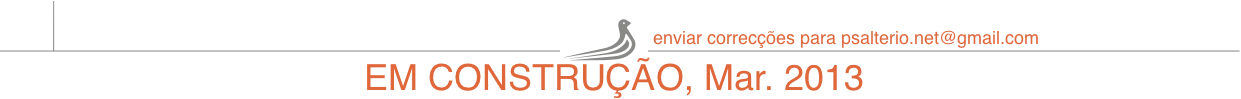
\includegraphics{_images/bkground_page_bottom.png}
}}





% this includes all the guitar tabs that may be needed
% must complete all the chords used in psalterio

% Cb chords

% C chords
\def \gtabCb{\gtab{Cb}{X32010:X32010}}
\def \gtabC{\gtab{C}{X32010:032010}}
\def \gtabCm{\gtab{Cm}{3:113321:004320}}

\def \gtabCsharpSusFour{\gtab{C\#sus4}{4:XX3341:XX2341}}

% Db chords

% D chords
\def \gtabD{\gtab{D}{X00232:000132}}
\def \gtabDm{\gtab{Dm}{X00231:000231}}
\def \gtabDfour{\gtab{D4}{X00233:000134}}
\def \gtabDseven{\gtab{D7}{X00212:000213}}
\def \gtabDsevenPlus{\gtab{D7+}{X00222:000111}}

% D#/Eb chords
\def \gtabDsharp{\gtab{D\#}{2:XX0232:000132}}

% E chords
\def \gtabE{\gtab{E}{022100:023100}}
\def \gtabEseven{\gtab{E}{020100:020100}}

\def \gtabEm{\gtab{Em}{022000:012000}}
\def \gtabEmSeven{\gtab{Em7}{022030:012040}}

% Gb chords

% F chords
\def \gtabF{\gtab{F}{1:133211:034200}}
\def \gtabFm{\gtab{Fm}{1:133111:034000}}


% F# chords
\def \gtabFsharpMinor{\gtab{F\#m}{2:133111:034000}}
\def \gtabFsharpMinorSeven{\gtab{F\#m7}{2:131131:030040}}

% Gb chords

% G chords
\def \gtabG{\gtab{G}{320033:210034}}
\def \gtabGseven{\gtab{G7}{320001:320001}}
\def \gtabGfret{\gtab{(G)}{3:133211:034200}}
\def \gtabGm{\gtab{Gm}{3:133111:034000}}


% G# / Ab chords

% A chords
\def \gtabA{\gtab{A}{X02220:001230}}
\def \gtabAm{\gtab{Am}{X02210:002310}}
\def \gtabAmSeven{\gtab{Am7}{X02010:002010}}
\def \gtabAfour{\gtab{A4}{X02230:001230}}
\def \gtabAseven{\gtab{A7}{X02020:001030}}

% Bb chords
\def \gtabBb{\gtab{Bb}{X13331}}

% B chords
\def \gtabB{\gtab{B}{X13331:003210}}
\def \gtabBm{\gtab{Bm}{X13321:003420}}
\def \gtabBmSeven{\gtab{Bm7}{X13121:003020}}



% after any { or } at the end of a line inside the macro definition add %, otherwise you'll get an extra space
\newcommand{\guitarTab}[1]{%
\ifstrequal{#1}{Cb}      {\gtab{Cb}{X32010:X32010}      }{}%
\ifstrequal{#1}{C}        { \gtab{C}{X32010:032010}       }{}%
%
%G
%
\ifstrequal{#1}{G}       { \gtab{G}{320033:210034}       }{}%
\ifstrequal{#1}{G7}     { \gtab{G7}{320001:320001}     }{}%
\ifstrequal{#1}{Gfret}  { \gtab{G}{3:133211:034200}    }{}%
\ifstrequal{#1}{Gm}    { \gtab{Gm}{3:133111:034000}  }{}%
} %end \newcommand{\gtab}

%muda aqui o numero da musica em que estas a trabalhar
%\def \selectSong{114}

\providebool{gchords}
\setbool{gchords}{true}

% set guitar chords vertical space separation with lyrics
\def \gchordsVspace{5 mm}

\begin{document}
	
	
	\AddToShipoutPicture*{\BottomPic}
	
	\begin{songs}{}
	
	%format file
	%
%Font Sizes
%
%\tiny
%\scriptsize
%\footnotesize
%\small
%\normalsize
%\large
%\Large
%\LARGE
%\huge
%\Huge


%\renewcommand{\thesongnum}{A\arabic{songnum}}
\renewcommand{\printsongnum}[1]{\sffamily\bfseries\huge\MakeUppercase#1}
\setlength{\songnumwidth}{2cm} % box width
%\renewcommand{\snumbgcolor}{white}

%change font for Title
\renewcommand{\stitlefont}{\sffamily\bfseries\huge\MakeUppercase} %song title

%remove verse numbers
%\noversenumbers 
% make left separation
\setlength{\versenumwidth}{2.0cm}

%verse separations
%\versesep=15pt
%\afterpreludeskip=2pt
%\beforepostludeskip=2pt
%\baselineadj=10pt

% separation between chords and lyrics
\renewcommand{\clineparams}{ 
\baselineskip=10pt 
%\lineskiplimit=2pt 
%\lineskip=5pt
}

% change font for lyrics
%\renewcommand{\lyricfont}{\sffamily}
%\renewcommand{\lyricfont}{\sffamily\small}
\renewcommand{\lyricfont}{\sffamily\large}
%\renewcommand{\chorusfont}{\sffamily}
\renewcommand{\chorusfont}{\sffamily\large}

%change the Chords formatting
\renewcommand{\printchord}[1]{\sffamily\color{red}\it\normalsize#1}

%check http://www.tug.org/pracjourn/2006-1/schmidt/schmidt.pdf


%\renewcommand{\songauthors}[1]{tete #1}


%\renewcommand{\extendpostlude}
%{ \songcopyright\ \songlicense\unskip \ Used with permission.}

\setlength{\cbarwidth}{0pt}
\setlength{\sbarheight}{0pt}

% music anf lyrics by
\newcommand{\musicLyricsBy}{} 
\newsongkey{mlby}{\def\musicLyricsBy{}}
                 {\def\musicLyricsBy{\sffamily\it\small letra e música por #1\par}}

% music anf lyrics by
\newcommand{\musicby}{} 
\newsongkey{music}{\def\musicby{}}
                 {\def\musicby{\sffamily\it\small música: #1\par}}

% music anf lyrics by
\newcommand{\lyricsby}{} 
\newsongkey{lyrics}{\def\lyricsby{}}
                 {\def\lyricsby{\sffamily\it\small letra: #1\par}}

%\renewcommand{\sharpsymbol}{\ensuremath{^\sharp}}
\renewcommand{\extendprelude}{
  \showrefs\showauthors 
  %{\bfseries\musicLyricsBy}
  {\bfseries\musicby}
  {\bfseries\lyricsby}
}

\def \gtabsOn{1}
	

%%%%%%%%%%%%%%%%%%%%%%%%%%%%%%%%%%%%%%%%%%%%%%%%%%%%%%%%%%%%%%%%%%%%%%%%%%%
% set song number
%%%%%%%%%%%%%%%%%%%%%%%%%%%%%%%%%%%%%%%%%%%%%%%%%%%%%%%%%%%%%%%%%%%%%%%%%%%
\setcounter{songnum}{15}       % song number

%%%%%%%%%%%%%%%%%%%%%%%%%%%%%%%%%%%%%%%%%%%%%%%%%%%%%%%%%%%%%%%%%%%%%%%%%%%
% begin song latex formating, set the title and other info
%%%%%%%%%%%%%%%%%%%%%%%%%%%%%%%%%%%%%%%%%%%%%%%%%%%%%%%%%%%%%%%%%%%%%%%%%%%
\beginsong{Caminhando}[            % song title ...
    %mlby={},                           % music and lyric by
    %sr={Revelation 5:13},        % bible verse
    %cr={Public domain.},         % licence
    %arr={my},                          % arrangement by
    index={Caminhando}]               % index title ...	

%%%%%%%%%%%%%%%%%%%%%%%%%%%%%%%%%%%%%%%%%%%%%%%%%%%%%%%%%%%%%%%%%%%%%%%%%%%
% verse #1
%%%%%%%%%%%%%%%%%%%%%%%%%%%%%%%%%%%%%%%%%%%%%%%%%%%%%%%%%%%%%%%%%%%%%%%%%%%
\beginverse                       % start verse

\[C]Com gozo eu ja vou para o lar celes\[G7]tial;
                         
Caminhando, ca\[C]minhando.
                                                                
Pois, nao me encanta mais o prazer te\[G7]rrenal,
                                        
Caminhando para aquele\[C] lar.

\endverse                         % end verse

%%%%%%%%%%%%%%%%%%%%%%%%%%%%%%%%%%%%%%%%%%%%%%%%%%%%%%%%%%%%%%%%%%%%%%%%%%%
% verse #2
%%%%%%%%%%%%%%%%%%%%%%%%%%%%%%%%%%%%%%%%%%%%%%%%%%%%%%%%%%%%%%%%%%%%%%%%%%%
\beginverse                       % start verse

Caminhando, cami\[Dm]nhan\[G7]do para aquele lar,
                    
Onde esta Je\[C]sus.
                            
Caminhando, cami\[Dm]nhando,
        
Pela \[G7]mao divina de Je\[C]sus.

\endverse                         % end verse

%%%%%%%%%%%%%%%%%%%%%%%%%%%%%%%%%%%%%%%%%%%%%%%%%%%%%%%%%%%%%%%%%%%%%%%%%%%
% verse #3
%%%%%%%%%%%%%%%%%%%%%%%%%%%%%%%%%%%%%%%%%%%%%%%%%%%%%%%%%%%%%%%%%%%%%%%%%%%
\beginverse                       % start verse

\[C]Eu quero pecadores comigo le\[G7]var;

Caminhando, ca\[C]minhando.

Que em Cristo possam eles saude en\[G7]contrar,

Caminhando para aquele\[C] lar.

\endverse                         % end verse

%%%%%%%%%%%%%%%%%%%%%%%%%%%%%%%%%%%%%%%%%%%%%%%%%%%%%%%%%%%%%%%%%%%%%%%%%%%
% verse #4
%%%%%%%%%%%%%%%%%%%%%%%%%%%%%%%%%%%%%%%%%%%%%%%%%%%%%%%%%%%%%%%%%%%%%%%%%%%
\beginverse                       % start verse

\[C]E entao com meu Jesus para sempre esta\[G7]rei;

Caminhando, ca\[C]minhando.

Seu nome eternamente entao lou\[G7]varei,

Caminhando, sim, naquele\[C] lar.

\endverse                         % start verse

%%%%%%%%%%%%%%%%%%%%%%%%%%%%%%%%%%%%%%%%%%%%%%%%%%%%%%%%%%%%%%%%%%%%%%%%%%%
% print guitar tabs used in this song
%%%%%%%%%%%%%%%%%%%%%%%%%%%%%%%%%%%%%%%%%%%%%%%%%%%%%%%%%%%%%%%%%%%%%%%%%%%
\ifbool{gchords}{                 % if the guitar chords are to be printed
\vspace{\gchordsVspace}           % set a vertical space of 10 pt 

\gtabC
\gtabF
%\gtabGseven
\gtabFsharpMinor
\gtabBm

}                                 % end if

%%%%%%%%%%%%%%%%%%%%%%%%%%%%%%%%%%%%%%%%%%%%%%%%%%%%%%%%%%%%%%%%%%%%%%%%%%%
% end song latex formating
%%%%%%%%%%%%%%%%%%%%%%%%%%%%%%%%%%%%%%%%%%%%%%%%%%%%%%%%%%%%%%%%%%%%%%%%%%%
\endsong                          % end song
%	 %lilypond-book --output=out --pdf  106single.tex
	 %\lilypondfile[]{E_101.ly}
	
\end{document}
	% percentagem é comentário
% 1 - \setcounter{songnum}{0} - numero da musica
% 2 - \beginsong{Viste quando?}[ - título da música
% 3 -  index={Viste quando?}] - entrada do indice da musica
% 4 - \beginverse , depois desta linha adicionar a letra
%%%%%%%%%%%%%%%%%%%%%%%%%%%%%%%%%%%%%%%%%%%%%%%%%%%%%%%%%%%%%%%%%%%%%%%%%%%
% this has all the necessary packages and formatting for the document
%%%%%%%%%%%%%%%%%%%%%%%%%%%%%%%%%%%%%%%%%%%%%%%%%%%%%%%%%%%%%%%%%%%%%%%%%%%
%\def \includeFolder{../_include}

% this has all the necessary packages and formatting for the document
\documentclass[10pt,a5paper]{article}

%define include folder
\def \includeFolder{_include}

%packages
\usepackage[left=1cm,right=1cm,top=1cm,bottom=1cm]{geometry}

\usepackage[chorded]{\includeFolder/psalterio} %must check the licence to change the name of the sty file!!!
%\usepackage[chorded]{resources/songs-old} %must check the licence to change the name of the sty file!!!

\usepackage[utf8]{inputenc}

\usepackage{graphicx}
\usepackage{wrapfig}
\usepackage{wallpaper}
\usepackage{color}
\usepackage{eso-pic} %for background pictures
\usepackage[bookmarks]{hyperref} 
%\usepackage{ifthen} %etoolbox is more up to date
\usepackage{etoolbox}


%\usepackage[xetex]{graphicx}
%\usepackage{fontspec,xunicode}
%\defaultfontfeatures{Mapping=tex-text,Scale=MatchLowercase}
%\setmainfont[Scale=.95]{Times}
%\setmonofont{Lucida Sans Typewriter}

%\usepackage[portuguese]{babel}
%\usepackage[latin1]{inputenc}
%\usepackage[utf8]{inputenc}
%\usepackage[T1]{fontenc}
%\usepackage[scaled]{uarial}
%\usepackage{helvet}
%\renewcommand{\familydefault}{\sfdefault}

%this removes the page number
\thispagestyle{empty}
\pagestyle{empty}
\songcolumns{1}

\parindent 0pt

%add background picture
\newcommand\BackgroundPic{
\put(0,0){
\parbox[b][\paperheight]{\paperwidth}{%
\vfill
\centering

\includegraphics[width=\paperwidth,height=\paperheight,
keepaspectratio]{logo.png}%
\vfill
}}}

\newcommand\BottomPic{
\put(0,0){
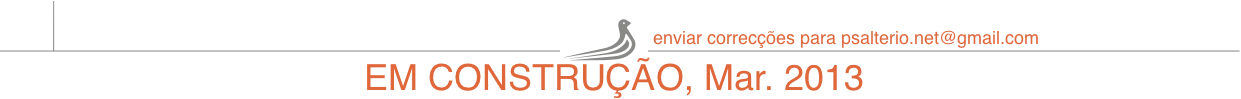
\includegraphics{_images/bkground_page_bottom.png}
}}





% this includes all the guitar tabs that may be needed
% must complete all the chords used in psalterio

% Cb chords

% C chords
\def \gtabCb{\gtab{Cb}{X32010:X32010}}
\def \gtabC{\gtab{C}{X32010:032010}}
\def \gtabCm{\gtab{Cm}{3:113321:004320}}

\def \gtabCsharpSusFour{\gtab{C\#sus4}{4:XX3341:XX2341}}

% Db chords

% D chords
\def \gtabD{\gtab{D}{X00232:000132}}
\def \gtabDm{\gtab{Dm}{X00231:000231}}
\def \gtabDfour{\gtab{D4}{X00233:000134}}
\def \gtabDseven{\gtab{D7}{X00212:000213}}
\def \gtabDsevenPlus{\gtab{D7+}{X00222:000111}}

% D#/Eb chords
\def \gtabDsharp{\gtab{D\#}{2:XX0232:000132}}

% E chords
\def \gtabE{\gtab{E}{022100:023100}}
\def \gtabEseven{\gtab{E}{020100:020100}}

\def \gtabEm{\gtab{Em}{022000:012000}}
\def \gtabEmSeven{\gtab{Em7}{022030:012040}}

% Gb chords

% F chords
\def \gtabF{\gtab{F}{1:133211:034200}}
\def \gtabFm{\gtab{Fm}{1:133111:034000}}


% F# chords
\def \gtabFsharpMinor{\gtab{F\#m}{2:133111:034000}}
\def \gtabFsharpMinorSeven{\gtab{F\#m7}{2:131131:030040}}

% Gb chords

% G chords
\def \gtabG{\gtab{G}{320033:210034}}
\def \gtabGseven{\gtab{G7}{320001:320001}}
\def \gtabGfret{\gtab{(G)}{3:133211:034200}}
\def \gtabGm{\gtab{Gm}{3:133111:034000}}


% G# / Ab chords

% A chords
\def \gtabA{\gtab{A}{X02220:001230}}
\def \gtabAm{\gtab{Am}{X02210:002310}}
\def \gtabAmSeven{\gtab{Am7}{X02010:002010}}
\def \gtabAfour{\gtab{A4}{X02230:001230}}
\def \gtabAseven{\gtab{A7}{X02020:001030}}

% Bb chords
\def \gtabBb{\gtab{Bb}{X13331}}

% B chords
\def \gtabB{\gtab{B}{X13331:003210}}
\def \gtabBm{\gtab{Bm}{X13321:003420}}
\def \gtabBmSeven{\gtab{Bm7}{X13121:003020}}



% after any { or } at the end of a line inside the macro definition add %, otherwise you'll get an extra space
\newcommand{\guitarTab}[1]{%
\ifstrequal{#1}{Cb}      {\gtab{Cb}{X32010:X32010}      }{}%
\ifstrequal{#1}{C}        { \gtab{C}{X32010:032010}       }{}%
%
%G
%
\ifstrequal{#1}{G}       { \gtab{G}{320033:210034}       }{}%
\ifstrequal{#1}{G7}     { \gtab{G7}{320001:320001}     }{}%
\ifstrequal{#1}{Gfret}  { \gtab{G}{3:133211:034200}    }{}%
\ifstrequal{#1}{Gm}    { \gtab{Gm}{3:133111:034000}  }{}%
} %end \newcommand{\gtab}

%muda aqui o numero da musica em que estas a trabalhar
%\def \selectSong{114}

\providebool{gchords}
\setbool{gchords}{true}

% set guitar chords vertical space separation with lyrics
\def \gchordsVspace{5 mm}

\begin{document}
	
	
	\AddToShipoutPicture*{\BottomPic}
	
	\begin{songs}{}
	
	%format file
	%
%Font Sizes
%
%\tiny
%\scriptsize
%\footnotesize
%\small
%\normalsize
%\large
%\Large
%\LARGE
%\huge
%\Huge


%\renewcommand{\thesongnum}{A\arabic{songnum}}
\renewcommand{\printsongnum}[1]{\sffamily\bfseries\huge\MakeUppercase#1}
\setlength{\songnumwidth}{2cm} % box width
%\renewcommand{\snumbgcolor}{white}

%change font for Title
\renewcommand{\stitlefont}{\sffamily\bfseries\huge\MakeUppercase} %song title

%remove verse numbers
%\noversenumbers 
% make left separation
\setlength{\versenumwidth}{2.0cm}

%verse separations
%\versesep=15pt
%\afterpreludeskip=2pt
%\beforepostludeskip=2pt
%\baselineadj=10pt

% separation between chords and lyrics
\renewcommand{\clineparams}{ 
\baselineskip=10pt 
%\lineskiplimit=2pt 
%\lineskip=5pt
}

% change font for lyrics
%\renewcommand{\lyricfont}{\sffamily}
%\renewcommand{\lyricfont}{\sffamily\small}
\renewcommand{\lyricfont}{\sffamily\large}
%\renewcommand{\chorusfont}{\sffamily}
\renewcommand{\chorusfont}{\sffamily\large}

%change the Chords formatting
\renewcommand{\printchord}[1]{\sffamily\color{red}\it\normalsize#1}

%check http://www.tug.org/pracjourn/2006-1/schmidt/schmidt.pdf


%\renewcommand{\songauthors}[1]{tete #1}


%\renewcommand{\extendpostlude}
%{ \songcopyright\ \songlicense\unskip \ Used with permission.}

\setlength{\cbarwidth}{0pt}
\setlength{\sbarheight}{0pt}

% music anf lyrics by
\newcommand{\musicLyricsBy}{} 
\newsongkey{mlby}{\def\musicLyricsBy{}}
                 {\def\musicLyricsBy{\sffamily\it\small letra e música por #1\par}}

% music anf lyrics by
\newcommand{\musicby}{} 
\newsongkey{music}{\def\musicby{}}
                 {\def\musicby{\sffamily\it\small música: #1\par}}

% music anf lyrics by
\newcommand{\lyricsby}{} 
\newsongkey{lyrics}{\def\lyricsby{}}
                 {\def\lyricsby{\sffamily\it\small letra: #1\par}}

%\renewcommand{\sharpsymbol}{\ensuremath{^\sharp}}
\renewcommand{\extendprelude}{
  \showrefs\showauthors 
  %{\bfseries\musicLyricsBy}
  {\bfseries\musicby}
  {\bfseries\lyricsby}
}

\def \gtabsOn{1}
	

%%%%%%%%%%%%%%%%%%%%%%%%%%%%%%%%%%%%%%%%%%%%%%%%%%%%%%%%%%%%%%%%%%%%%%%%%%%
% set song number
%%%%%%%%%%%%%%%%%%%%%%%%%%%%%%%%%%%%%%%%%%%%%%%%%%%%%%%%%%%%%%%%%%%%%%%%%%%
\setcounter{songnum}{16}       % song number

%%%%%%%%%%%%%%%%%%%%%%%%%%%%%%%%%%%%%%%%%%%%%%%%%%%%%%%%%%%%%%%%%%%%%%%%%%%
% begin song latex formating, set the title and other info
%%%%%%%%%%%%%%%%%%%%%%%%%%%%%%%%%%%%%%%%%%%%%%%%%%%%%%%%%%%%%%%%%%%%%%%%%%%
\beginsong{Viste Quando}[            % song title ...
    %mlby={},                           % music and lyric by
    %sr={Revelation 5:13},        % bible verse
    %cr={Public domain.},         % licence
    %arr={my},                          % arrangement by
    index={Viste Quando}]               % index title ...	

%%%%%%%%%%%%%%%%%%%%%%%%%%%%%%%%%%%%%%%%%%%%%%%%%%%%%%%%%%%%%%%%%%%%%%%%%%%
% verse #1
%%%%%%%%%%%%%%%%%%%%%%%%%%%%%%%%%%%%%%%%%%%%%%%%%%%%%%%%%%%%%%%%%%%%%%%%%%%
\beginverse                       % start verse

\[Eb]Viste quando o Se\[Bb]nhor \[Cm]mo\[Gm]rreu \[Bb7]na c\[Eb]ruz?

Viste \[Gm]quan\[Bb]do o Se\[Cm]nhor mo\[Bb]rreu \[Eb]na c\[Bb]ruz?

\[Eb]Oh! \[Ab]As \[Eb]ve\[Ab]zes \[Eb]tenho \[G]pena e\[Cm] tremo,\[Ab] tremo, tr\[Eb]emo,\[Ab]\[Bb]

\[Ab]Viste \[Eb]quando o Se\[Bb]nhor \[Cm]mo\[Gm]rreu n\[Bb7]a cr\[Eb]uz?

\endverse                         % end verse

%%%%%%%%%%%%%%%%%%%%%%%%%%%%%%%%%%%%%%%%%%%%%%%%%%%%%%%%%%%%%%%%%%%%%%%%%%%
% verse #2
%%%%%%%%%%%%%%%%%%%%%%%%%%%%%%%%%%%%%%%%%%%%%%%%%%%%%%%%%%%%%%%%%%%%%%%%%%%
\beginverse                       % start verse

\[Eb]Viste quando O pre\[Bb]ga\[Cm]ram\[Gm] nu\[Bb7]ma c\[Eb]ruz?

Viste \[Gm]quan\[Bb]do O pre\[Cm]garam\[Bb] nu\[Eb]ma c\[Bb]ruz?
 
\[Eb]Oh! \[Ab]As \[Eb]ve\[Ab]zes \[Eb]tenho \[G]pena e\[Cm] tremo,\[Ab] tremo, tr\[Eb]emo,\[Ab]\[Bb]

\[Ab]Viste \[Eb]quando O pre\[Bb]ga\[Cm]ram\[Gm] nu\[Bb7]ma c\[Eb]ruz?

\endverse                         % end verse

%%%%%%%%%%%%%%%%%%%%%%%%%%%%%%%%%%%%%%%%%%%%%%%%%%%%%%%%%%%%%%%%%%%%%%%%%%%
% verse #3
%%%%%%%%%%%%%%%%%%%%%%%%%%%%%%%%%%%%%%%%%%%%%%%%%%%%%%%%%%%%%%%%%%%%%%%%%%%
\beginverse                       % start verse

\[Eb]Viste quando p'ra \[Bb]tum\[Cm]ba \[Gm]foi \[Bb7]Je\[Eb]sus?

Viste \[Gm]quan\[Bb]do p'ra \[Cm]tumba \[Bb]foi \[Eb]Je\[Bb]sus? 

\[Eb]Oh! \[Ab]As \[Eb]ve\[Ab]zes \[Eb]tenho \[G]pena e\[Cm] tremo,\[Ab] tremo, tr\[Eb]emo,\[Ab]\[Bb]

\[Ab]Viste \[Eb]quando p'ra \[Bb]tum\[Cm]ba \[Gm]foi \[Bb7]Je\[Eb]sus?

\endverse                         % end verse

%%%%%%%%%%%%%%%%%%%%%%%%%%%%%%%%%%%%%%%%%%%%%%%%%%%%%%%%%%%%%%%%%%%%%%%%%%%
% verse #4
%%%%%%%%%%%%%%%%%%%%%%%%%%%%%%%%%%%%%%%%%%%%%%%%%%%%%%%%%%%%%%%%%%%%%%%%%%%
\beginverse                       % start verse

\[Eb]Viste quando o Se\[Bb]nhor \[Cm]re\[Gm]ssus\[Bb7]ci\[Eb]tou?

Viste \[Gm]quan\[Bb]do o Se\[Cm]nhor re\[Bb]ssus\[Eb]ci\[Bb]tou?

\[Eb]Oh! \[Ab]As \[Eb]ve\[Ab]zes \[Eb]tenho \[G]pena e\[Cm] tremo,\[Ab] tremo, tr\[Eb]emo,\[Ab]\[Bb]

\[Ab]Viste \[Eb]quando o Se\[Bb]nhor \[Cm]re\[Gm]ssus\[Bb7]ci\[Eb]tou?

\endverse                         % start verse

%%%%%%%%%%%%%%%%%%%%%%%%%%%%%%%%%%%%%%%%%%%%%%%%%%%%%%%%%%%%%%%%%%%%%%%%%%%
% print guitar tabs used in this song
%%%%%%%%%%%%%%%%%%%%%%%%%%%%%%%%%%%%%%%%%%%%%%%%%%%%%%%%%%%%%%%%%%%%%%%%%%%
\ifbool{gchords}{                 % if the guitar chords are to be printed
\vspace{\gchordsVspace}           % set a vertical space of 10 pt 

\gtabC
\gtabF
%\gtabGseven
\gtabFsharpMinor
\gtabBm

}                                 % end if

%%%%%%%%%%%%%%%%%%%%%%%%%%%%%%%%%%%%%%%%%%%%%%%%%%%%%%%%%%%%%%%%%%%%%%%%%%%
% end song latex formating
%%%%%%%%%%%%%%%%%%%%%%%%%%%%%%%%%%%%%%%%%%%%%%%%%%%%%%%%%%%%%%%%%%%%%%%%%%%
\endsong                          % end song
%	 %lilypond-book --output=out --pdf  106single.tex
	 %\lilypondfile[]{E_101.ly}
	
\end{document}
	%%%%%%%%%%%%%%%%%%%%%%%%%%%%%%%%%%%%%%%%%%%%%%%%%%%%%%%%%%%%%%%%%%%%%%%%%%%
% this has all the necessary packages and formatting for the document
%%%%%%%%%%%%%%%%%%%%%%%%%%%%%%%%%%%%%%%%%%%%%%%%%%%%%%%%%%%%%%%%%%%%%%%%%%%
%\def \includeFolder{../_include}

% this has all the necessary packages and formatting for the document
\documentclass[10pt,a5paper]{article}

%define include folder
\def \includeFolder{_include}

%packages
\usepackage[left=1cm,right=1cm,top=1cm,bottom=1cm]{geometry}

\usepackage[chorded]{\includeFolder/psalterio} %must check the licence to change the name of the sty file!!!
%\usepackage[chorded]{resources/songs-old} %must check the licence to change the name of the sty file!!!

\usepackage[utf8]{inputenc}

\usepackage{graphicx}
\usepackage{wrapfig}
\usepackage{wallpaper}
\usepackage{color}
\usepackage{eso-pic} %for background pictures
\usepackage[bookmarks]{hyperref} 
%\usepackage{ifthen} %etoolbox is more up to date
\usepackage{etoolbox}


%\usepackage[xetex]{graphicx}
%\usepackage{fontspec,xunicode}
%\defaultfontfeatures{Mapping=tex-text,Scale=MatchLowercase}
%\setmainfont[Scale=.95]{Times}
%\setmonofont{Lucida Sans Typewriter}

%\usepackage[portuguese]{babel}
%\usepackage[latin1]{inputenc}
%\usepackage[utf8]{inputenc}
%\usepackage[T1]{fontenc}
%\usepackage[scaled]{uarial}
%\usepackage{helvet}
%\renewcommand{\familydefault}{\sfdefault}

%this removes the page number
\thispagestyle{empty}
\pagestyle{empty}
\songcolumns{1}

\parindent 0pt

%add background picture
\newcommand\BackgroundPic{
\put(0,0){
\parbox[b][\paperheight]{\paperwidth}{%
\vfill
\centering

\includegraphics[width=\paperwidth,height=\paperheight,
keepaspectratio]{logo.png}%
\vfill
}}}

\newcommand\BottomPic{
\put(0,0){
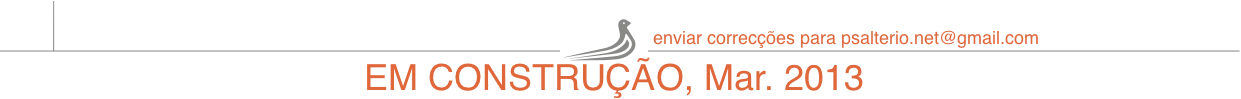
\includegraphics{_images/bkground_page_bottom.png}
}}





% this includes all the guitar tabs that may be needed
% must complete all the chords used in psalterio

% Cb chords

% C chords
\def \gtabCb{\gtab{Cb}{X32010:X32010}}
\def \gtabC{\gtab{C}{X32010:032010}}
\def \gtabCm{\gtab{Cm}{3:113321:004320}}

\def \gtabCsharpSusFour{\gtab{C\#sus4}{4:XX3341:XX2341}}

% Db chords

% D chords
\def \gtabD{\gtab{D}{X00232:000132}}
\def \gtabDm{\gtab{Dm}{X00231:000231}}
\def \gtabDfour{\gtab{D4}{X00233:000134}}
\def \gtabDseven{\gtab{D7}{X00212:000213}}
\def \gtabDsevenPlus{\gtab{D7+}{X00222:000111}}

% D#/Eb chords
\def \gtabDsharp{\gtab{D\#}{2:XX0232:000132}}

% E chords
\def \gtabE{\gtab{E}{022100:023100}}
\def \gtabEseven{\gtab{E}{020100:020100}}

\def \gtabEm{\gtab{Em}{022000:012000}}
\def \gtabEmSeven{\gtab{Em7}{022030:012040}}

% Gb chords

% F chords
\def \gtabF{\gtab{F}{1:133211:034200}}
\def \gtabFm{\gtab{Fm}{1:133111:034000}}


% F# chords
\def \gtabFsharpMinor{\gtab{F\#m}{2:133111:034000}}
\def \gtabFsharpMinorSeven{\gtab{F\#m7}{2:131131:030040}}

% Gb chords

% G chords
\def \gtabG{\gtab{G}{320033:210034}}
\def \gtabGseven{\gtab{G7}{320001:320001}}
\def \gtabGfret{\gtab{(G)}{3:133211:034200}}
\def \gtabGm{\gtab{Gm}{3:133111:034000}}


% G# / Ab chords

% A chords
\def \gtabA{\gtab{A}{X02220:001230}}
\def \gtabAm{\gtab{Am}{X02210:002310}}
\def \gtabAmSeven{\gtab{Am7}{X02010:002010}}
\def \gtabAfour{\gtab{A4}{X02230:001230}}
\def \gtabAseven{\gtab{A7}{X02020:001030}}

% Bb chords
\def \gtabBb{\gtab{Bb}{X13331}}

% B chords
\def \gtabB{\gtab{B}{X13331:003210}}
\def \gtabBm{\gtab{Bm}{X13321:003420}}
\def \gtabBmSeven{\gtab{Bm7}{X13121:003020}}



% after any { or } at the end of a line inside the macro definition add %, otherwise you'll get an extra space
\newcommand{\guitarTab}[1]{%
\ifstrequal{#1}{Cb}      {\gtab{Cb}{X32010:X32010}      }{}%
\ifstrequal{#1}{C}        { \gtab{C}{X32010:032010}       }{}%
%
%G
%
\ifstrequal{#1}{G}       { \gtab{G}{320033:210034}       }{}%
\ifstrequal{#1}{G7}     { \gtab{G7}{320001:320001}     }{}%
\ifstrequal{#1}{Gfret}  { \gtab{G}{3:133211:034200}    }{}%
\ifstrequal{#1}{Gm}    { \gtab{Gm}{3:133111:034000}  }{}%
} %end \newcommand{\gtab}

%muda aqui o numero da musica em que estas a trabalhar
%\def \selectSong{114}

\providebool{gchords}
\setbool{gchords}{true}

% set guitar chords vertical space separation with lyrics
\def \gchordsVspace{5 mm}

\begin{document}
	
	
	\AddToShipoutPicture*{\BottomPic}
	
	\begin{songs}{}
	
	%format file
	%
%Font Sizes
%
%\tiny
%\scriptsize
%\footnotesize
%\small
%\normalsize
%\large
%\Large
%\LARGE
%\huge
%\Huge


%\renewcommand{\thesongnum}{A\arabic{songnum}}
\renewcommand{\printsongnum}[1]{\sffamily\bfseries\huge\MakeUppercase#1}
\setlength{\songnumwidth}{2cm} % box width
%\renewcommand{\snumbgcolor}{white}

%change font for Title
\renewcommand{\stitlefont}{\sffamily\bfseries\huge\MakeUppercase} %song title

%remove verse numbers
%\noversenumbers 
% make left separation
\setlength{\versenumwidth}{2.0cm}

%verse separations
%\versesep=15pt
%\afterpreludeskip=2pt
%\beforepostludeskip=2pt
%\baselineadj=10pt

% separation between chords and lyrics
\renewcommand{\clineparams}{ 
\baselineskip=10pt 
%\lineskiplimit=2pt 
%\lineskip=5pt
}

% change font for lyrics
%\renewcommand{\lyricfont}{\sffamily}
%\renewcommand{\lyricfont}{\sffamily\small}
\renewcommand{\lyricfont}{\sffamily\large}
%\renewcommand{\chorusfont}{\sffamily}
\renewcommand{\chorusfont}{\sffamily\large}

%change the Chords formatting
\renewcommand{\printchord}[1]{\sffamily\color{red}\it\normalsize#1}

%check http://www.tug.org/pracjourn/2006-1/schmidt/schmidt.pdf


%\renewcommand{\songauthors}[1]{tete #1}


%\renewcommand{\extendpostlude}
%{ \songcopyright\ \songlicense\unskip \ Used with permission.}

\setlength{\cbarwidth}{0pt}
\setlength{\sbarheight}{0pt}

% music anf lyrics by
\newcommand{\musicLyricsBy}{} 
\newsongkey{mlby}{\def\musicLyricsBy{}}
                 {\def\musicLyricsBy{\sffamily\it\small letra e música por #1\par}}

% music anf lyrics by
\newcommand{\musicby}{} 
\newsongkey{music}{\def\musicby{}}
                 {\def\musicby{\sffamily\it\small música: #1\par}}

% music anf lyrics by
\newcommand{\lyricsby}{} 
\newsongkey{lyrics}{\def\lyricsby{}}
                 {\def\lyricsby{\sffamily\it\small letra: #1\par}}

%\renewcommand{\sharpsymbol}{\ensuremath{^\sharp}}
\renewcommand{\extendprelude}{
  \showrefs\showauthors 
  %{\bfseries\musicLyricsBy}
  {\bfseries\musicby}
  {\bfseries\lyricsby}
}

\def \gtabsOn{1}
	

%%%%%%%%%%%%%%%%%%%%%%%%%%%%%%%%%%%%%%%%%%%%%%%%%%%%%%%%%%%%%%%%%%%%%%%%%%%
% set song number
%%%%%%%%%%%%%%%%%%%%%%%%%%%%%%%%%%%%%%%%%%%%%%%%%%%%%%%%%%%%%%%%%%%%%%%%%%%
\setcounter{songnum}{17}

%%%%%%%%%%%%%%%%%%%%%%%%%%%%%%%%%%%%%%%%%%%%%%%%%%%%%%%%%%%%%%%%%%%%%%%%%%%
% begin song latex formating, set the title and other info
%%%%%%%%%%%%%%%%%%%%%%%%%%%%%%%%%%%%%%%%%%%%%%%%%%%%%%%%%%%%%%%%%%%%%%%%%%%
% song title
\beginsong{J’ai choisi de suivre Jésus-Christ}[
        % music and lyric by
        % mlby={},
        % lyrics
        lyrics={}, 
        % music by
        music={},
        % bible verse
        %sr={},
        % licence/copyright
        %cr={Public domain.},
        % arrangement by
        %arr={},
        % index title
        index={J’ai choisi de suivre Jésus-Christ}]

%%%%%%%%%%%%%%%%%%%%%%%%%%%%%%%%%%%%%%%%%%%%%%%%%%%%%%%%%%%%%%%%%%%%%%%%%%%
% section #1: verse 
%%%%%%%%%%%%%%%%%%%%%%%%%%%%%%%%%%%%%%%%%%%%%%%%%%%%%%%%%%%%%%%%%%%%%%%%%%%
\beginverse
En \[D]mon coeur, j’ai choisi \[G]de \[A7]suivre \[D]Jésus-Christ,
En \[D]mon coeur, \[G]j’ai choisi de suivre \[G]Jésus,
En mon coeur, j’ai choisi \[G]de \[D]suivre \[F#m]Jésus-\[Bm]Christ,
Oui, \[G]pour \[A7]tou\[Bm]jours, oui, \[Em]pour \[A7]tou\[D]jours.
\endverse

%%%%%%%%%%%%%%%%%%%%%%%%%%%%%%%%%%%%%%%%%%%%%%%%%%%%%%%%%%%%%%%%%%%%%%%%%%%
% section #2: verse 
%%%%%%%%%%%%%%%%%%%%%%%%%%%%%%%%%%%%%%%%%%%%%%%%%%%%%%%%%%%%%%%%%%%%%%%%%%%
\beginverse
Si mes amis s’en vont, qu’importe?Moi, j’irai!
Si mes amis s’en vont, qu’importe?J’irai!
Si mes amis s’en vont, qu’importe?Moi, j’irai!
Oui, pour toujours, oui, pour toujours.
\endverse

%%%%%%%%%%%%%%%%%%%%%%%%%%%%%%%%%%%%%%%%%%%%%%%%%%%%%%%%%%%%%%%%%%%%%%%%%%%
% section #3: verse 
%%%%%%%%%%%%%%%%%%%%%%%%%%%%%%%%%%%%%%%%%%%%%%%%%%%%%%%%%%%%%%%%%%%%%%%%%%%
\beginverse
Au mondeje dis “non”, joyeux je prends ma croix,
Au mondeje dis “non”, joyeux j’accepte la croix,
Au mondeje dis “non”, joyeux je prends ma croix,
Oui, pour toujours, oui, pour toujours.
\endverse


%%%%%%%%%%%%%%%%%%%%%%%%%%%%%%%%%%%%%%%%%%%%%%%%%%%%%%%%%%%%%%%%%%%%%%%%%%%
% print guitar tabs used in this song
%%%%%%%%%%%%%%%%%%%%%%%%%%%%%%%%%%%%%%%%%%%%%%%%%%%%%%%%%%%%%%%%%%%%%%%%%%%
% if the guitar chords are to be printed
\ifbool{gchords}{
% set a vertical space of 10 pt 
\vspace{\gchordsVspace}
} % end if

%%%%%%%%%%%%%%%%%%%%%%%%%%%%%%%%%%%%%%%%%%%%%%%%%%%%%%%%%%%%%%%%%%%%%%%%%%%
% end song latex formating
%%%%%%%%%%%%%%%%%%%%%%%%%%%%%%%%%%%%%%%%%%%%%%%%%%%%%%%%%%%%%%%%%%%%%%%%%%%
% end song
\endsong

%include song latex footer
%	 %lilypond-book --output=out --pdf  106single.tex
	 %\lilypondfile[]{E_101.ly}
	
\end{document}	
	% percentagem � coment�rio
% 1 - \setcounter{songnum}{0} - numero da musica
% 2 - \beginsong{Quando penso na cruz}[ - t�tulo da m�sica
% 3 -  index={Quando penso na cruz}] - entrada do indice da musica
% 4 - \beginverse , depois desta linha adicionar a letra
%%%%%%%%%%%%%%%%%%%%%%%%%%%%%%%%%%%%%%%%%%%%%%%%%%%%%%%%%%%%%%%%%%%%%%%%%%%
% this has all the necessary packages and formatting for the document
%%%%%%%%%%%%%%%%%%%%%%%%%%%%%%%%%%%%%%%%%%%%%%%%%%%%%%%%%%%%%%%%%%%%%%%%%%%
%\def \includeFolder{../_include}

% this has all the necessary packages and formatting for the document
\documentclass[10pt,a5paper]{article}

%define include folder
\def \includeFolder{_include}

%packages
\usepackage[left=1cm,right=1cm,top=1cm,bottom=1cm]{geometry}

\usepackage[chorded]{\includeFolder/psalterio} %must check the licence to change the name of the sty file!!!
%\usepackage[chorded]{resources/songs-old} %must check the licence to change the name of the sty file!!!

\usepackage[utf8]{inputenc}

\usepackage{graphicx}
\usepackage{wrapfig}
\usepackage{wallpaper}
\usepackage{color}
\usepackage{eso-pic} %for background pictures
\usepackage[bookmarks]{hyperref} 
%\usepackage{ifthen} %etoolbox is more up to date
\usepackage{etoolbox}


%\usepackage[xetex]{graphicx}
%\usepackage{fontspec,xunicode}
%\defaultfontfeatures{Mapping=tex-text,Scale=MatchLowercase}
%\setmainfont[Scale=.95]{Times}
%\setmonofont{Lucida Sans Typewriter}

%\usepackage[portuguese]{babel}
%\usepackage[latin1]{inputenc}
%\usepackage[utf8]{inputenc}
%\usepackage[T1]{fontenc}
%\usepackage[scaled]{uarial}
%\usepackage{helvet}
%\renewcommand{\familydefault}{\sfdefault}

%this removes the page number
\thispagestyle{empty}
\pagestyle{empty}
\songcolumns{1}

\parindent 0pt

%add background picture
\newcommand\BackgroundPic{
\put(0,0){
\parbox[b][\paperheight]{\paperwidth}{%
\vfill
\centering

\includegraphics[width=\paperwidth,height=\paperheight,
keepaspectratio]{logo.png}%
\vfill
}}}

\newcommand\BottomPic{
\put(0,0){
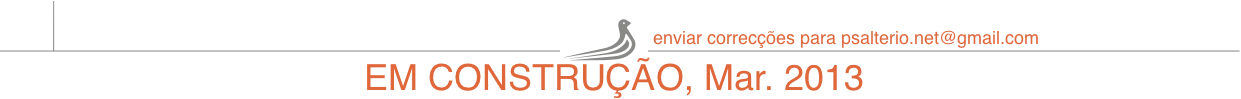
\includegraphics{_images/bkground_page_bottom.png}
}}





% this includes all the guitar tabs that may be needed
% must complete all the chords used in psalterio

% Cb chords

% C chords
\def \gtabCb{\gtab{Cb}{X32010:X32010}}
\def \gtabC{\gtab{C}{X32010:032010}}
\def \gtabCm{\gtab{Cm}{3:113321:004320}}

\def \gtabCsharpSusFour{\gtab{C\#sus4}{4:XX3341:XX2341}}

% Db chords

% D chords
\def \gtabD{\gtab{D}{X00232:000132}}
\def \gtabDm{\gtab{Dm}{X00231:000231}}
\def \gtabDfour{\gtab{D4}{X00233:000134}}
\def \gtabDseven{\gtab{D7}{X00212:000213}}
\def \gtabDsevenPlus{\gtab{D7+}{X00222:000111}}

% D#/Eb chords
\def \gtabDsharp{\gtab{D\#}{2:XX0232:000132}}

% E chords
\def \gtabE{\gtab{E}{022100:023100}}
\def \gtabEseven{\gtab{E}{020100:020100}}

\def \gtabEm{\gtab{Em}{022000:012000}}
\def \gtabEmSeven{\gtab{Em7}{022030:012040}}

% Gb chords

% F chords
\def \gtabF{\gtab{F}{1:133211:034200}}
\def \gtabFm{\gtab{Fm}{1:133111:034000}}


% F# chords
\def \gtabFsharpMinor{\gtab{F\#m}{2:133111:034000}}
\def \gtabFsharpMinorSeven{\gtab{F\#m7}{2:131131:030040}}

% Gb chords

% G chords
\def \gtabG{\gtab{G}{320033:210034}}
\def \gtabGseven{\gtab{G7}{320001:320001}}
\def \gtabGfret{\gtab{(G)}{3:133211:034200}}
\def \gtabGm{\gtab{Gm}{3:133111:034000}}


% G# / Ab chords

% A chords
\def \gtabA{\gtab{A}{X02220:001230}}
\def \gtabAm{\gtab{Am}{X02210:002310}}
\def \gtabAmSeven{\gtab{Am7}{X02010:002010}}
\def \gtabAfour{\gtab{A4}{X02230:001230}}
\def \gtabAseven{\gtab{A7}{X02020:001030}}

% Bb chords
\def \gtabBb{\gtab{Bb}{X13331}}

% B chords
\def \gtabB{\gtab{B}{X13331:003210}}
\def \gtabBm{\gtab{Bm}{X13321:003420}}
\def \gtabBmSeven{\gtab{Bm7}{X13121:003020}}



% after any { or } at the end of a line inside the macro definition add %, otherwise you'll get an extra space
\newcommand{\guitarTab}[1]{%
\ifstrequal{#1}{Cb}      {\gtab{Cb}{X32010:X32010}      }{}%
\ifstrequal{#1}{C}        { \gtab{C}{X32010:032010}       }{}%
%
%G
%
\ifstrequal{#1}{G}       { \gtab{G}{320033:210034}       }{}%
\ifstrequal{#1}{G7}     { \gtab{G7}{320001:320001}     }{}%
\ifstrequal{#1}{Gfret}  { \gtab{G}{3:133211:034200}    }{}%
\ifstrequal{#1}{Gm}    { \gtab{Gm}{3:133111:034000}  }{}%
} %end \newcommand{\gtab}

%muda aqui o numero da musica em que estas a trabalhar
%\def \selectSong{114}

\providebool{gchords}
\setbool{gchords}{true}

% set guitar chords vertical space separation with lyrics
\def \gchordsVspace{5 mm}

\begin{document}
	
	
	\AddToShipoutPicture*{\BottomPic}
	
	\begin{songs}{}
	
	%format file
	%
%Font Sizes
%
%\tiny
%\scriptsize
%\footnotesize
%\small
%\normalsize
%\large
%\Large
%\LARGE
%\huge
%\Huge


%\renewcommand{\thesongnum}{A\arabic{songnum}}
\renewcommand{\printsongnum}[1]{\sffamily\bfseries\huge\MakeUppercase#1}
\setlength{\songnumwidth}{2cm} % box width
%\renewcommand{\snumbgcolor}{white}

%change font for Title
\renewcommand{\stitlefont}{\sffamily\bfseries\huge\MakeUppercase} %song title

%remove verse numbers
%\noversenumbers 
% make left separation
\setlength{\versenumwidth}{2.0cm}

%verse separations
%\versesep=15pt
%\afterpreludeskip=2pt
%\beforepostludeskip=2pt
%\baselineadj=10pt

% separation between chords and lyrics
\renewcommand{\clineparams}{ 
\baselineskip=10pt 
%\lineskiplimit=2pt 
%\lineskip=5pt
}

% change font for lyrics
%\renewcommand{\lyricfont}{\sffamily}
%\renewcommand{\lyricfont}{\sffamily\small}
\renewcommand{\lyricfont}{\sffamily\large}
%\renewcommand{\chorusfont}{\sffamily}
\renewcommand{\chorusfont}{\sffamily\large}

%change the Chords formatting
\renewcommand{\printchord}[1]{\sffamily\color{red}\it\normalsize#1}

%check http://www.tug.org/pracjourn/2006-1/schmidt/schmidt.pdf


%\renewcommand{\songauthors}[1]{tete #1}


%\renewcommand{\extendpostlude}
%{ \songcopyright\ \songlicense\unskip \ Used with permission.}

\setlength{\cbarwidth}{0pt}
\setlength{\sbarheight}{0pt}

% music anf lyrics by
\newcommand{\musicLyricsBy}{} 
\newsongkey{mlby}{\def\musicLyricsBy{}}
                 {\def\musicLyricsBy{\sffamily\it\small letra e música por #1\par}}

% music anf lyrics by
\newcommand{\musicby}{} 
\newsongkey{music}{\def\musicby{}}
                 {\def\musicby{\sffamily\it\small música: #1\par}}

% music anf lyrics by
\newcommand{\lyricsby}{} 
\newsongkey{lyrics}{\def\lyricsby{}}
                 {\def\lyricsby{\sffamily\it\small letra: #1\par}}

%\renewcommand{\sharpsymbol}{\ensuremath{^\sharp}}
\renewcommand{\extendprelude}{
  \showrefs\showauthors 
  %{\bfseries\musicLyricsBy}
  {\bfseries\musicby}
  {\bfseries\lyricsby}
}

\def \gtabsOn{1}
	

%%%%%%%%%%%%%%%%%%%%%%%%%%%%%%%%%%%%%%%%%%%%%%%%%%%%%%%%%%%%%%%%%%%%%%%%%%%
% set song number
%%%%%%%%%%%%%%%%%%%%%%%%%%%%%%%%%%%%%%%%%%%%%%%%%%%%%%%%%%%%%%%%%%%%%%%%%%%
\setcounter{songnum}{18}       % song number

%%%%%%%%%%%%%%%%%%%%%%%%%%%%%%%%%%%%%%%%%%%%%%%%%%%%%%%%%%%%%%%%%%%%%%%%%%%
% begin song latex formating, set the title and other info
%%%%%%%%%%%%%%%%%%%%%%%%%%%%%%%%%%%%%%%%%%%%%%%%%%%%%%%%%%%%%%%%%%%%%%%%%%%
\beginsong{Quando Penso Na Cruz}[            % song title ...
    %mlby={},                           % music and lyric by
    %sr={Revelation 5:13},        % bible verse
    %cr={Public domain.},         % licence
    %arr={my},                          % arrangement by
    index={Quando Penso Na Cruz}]               % index title ...	

%%%%%%%%%%%%%%%%%%%%%%%%%%%%%%%%%%%%%%%%%%%%%%%%%%%%%%%%%%%%%%%%%%%%%%%%%%%
% verse #1
%%%%%%%%%%%%%%%%%%%%%%%%%%%%%%%%%%%%%%%%%%%%%%%%%%%%%%%%%%%%%%%%%%%%%%%%%%%
\beginverse                       % start verse

\[Ab]Foi numa cruz e num \[Bbm]tempo sem fim,

\[Eb7]Sons bem diferentes subiram aos \[Ab]ceus.
                           
Um homem la sus\[Db]penso ficou,
        
Sem \[Eb]culpa, inocente, por\[Db] mim pad\[Ab]eceu.

\endverse                         % end verse

%%%%%%%%%%%%%%%%%%%%%%%%%%%%%%%%%%%%%%%%%%%%%%%%%%%%%%%%%%%%%%%%%%%%%%%%%%%
% verse #2
%%%%%%%%%%%%%%%%%%%%%%%%%%%%%%%%%%%%%%%%%%%%%%%%%%%%%%%%%%%%%%%%%%%%%%%%%%%
\beginverse                       % start verse

\[C]Quando penso na cruz, \[Fm]tao cruel,
      
Seu \[C]sangue a cair, es\[Fm]pinhos fel,
      
Se \[C]penso na cruz, \[Fm]faz-me sentir,
   
O \[Gb]seu grande \[Db]amor em \[Bb]estar junto a \[Eb]mim,
   
As\[Ab]sim livre \[Bb]sou, livre \[Eb]sou, livre sou.

\endverse                         % end verse

%%%%%%%%%%%%%%%%%%%%%%%%%%%%%%%%%%%%%%%%%%%%%%%%%%%%%%%%%%%%%%%%%%%%%%%%%%%
% verse #3
%%%%%%%%%%%%%%%%%%%%%%%%%%%%%%%%%%%%%%%%%%%%%%%%%%%%%%%%%%%%%%%%%%%%%%%%%%%
\beginverse                       % start verse

\[Ab]Ele sarou minha cul\[Bbm]pa e dor,

\[Eb7]Em vez de odio, doce paz e a\[Ab]mor.

Perdao e vida ao ho\[Db]mem quis dar,

A\[Eb]fim de a vida eterna \[Db]encon\[Ab]trar.

\endverse                         % start verse

%%%%%%%%%%%%%%%%%%%%%%%%%%%%%%%%%%%%%%%%%%%%%%%%%%%%%%%%%%%%%%%%%%%%%%%%%%%
% print guitar tabs used in this song
%%%%%%%%%%%%%%%%%%%%%%%%%%%%%%%%%%%%%%%%%%%%%%%%%%%%%%%%%%%%%%%%%%%%%%%%%%%
\ifbool{gchords}{                 % if the guitar chords are to be printed
\vspace{\gchordsVspace}           % set a vertical space of 10 pt 

\gtabC
\gtabF
%\gtabGseven
\gtabFsharpMinor
\gtabBm

}                                 % end if

%%%%%%%%%%%%%%%%%%%%%%%%%%%%%%%%%%%%%%%%%%%%%%%%%%%%%%%%%%%%%%%%%%%%%%%%%%%
% end song latex formating
%%%%%%%%%%%%%%%%%%%%%%%%%%%%%%%%%%%%%%%%%%%%%%%%%%%%%%%%%%%%%%%%%%%%%%%%%%%
\endsong                          % end song
%	 %lilypond-book --output=out --pdf  106single.tex
	 %\lilypondfile[]{E_101.ly}
	
\end{document}
	%%%%%%%%%%%%%%%%%%%%%%%%%%%%%%%%%%%%%%%%%%%%%%%%%%%%%%%%%%%%%%%%%%%%%%%%%%%
% this has all the necessary packages and formatting for the document
%%%%%%%%%%%%%%%%%%%%%%%%%%%%%%%%%%%%%%%%%%%%%%%%%%%%%%%%%%%%%%%%%%%%%%%%%%%
%\def \includeFolder{../_include}

% this has all the necessary packages and formatting for the document
\documentclass[10pt,a5paper]{article}

%define include folder
\def \includeFolder{_include}

%packages
\usepackage[left=1cm,right=1cm,top=1cm,bottom=1cm]{geometry}

\usepackage[chorded]{\includeFolder/psalterio} %must check the licence to change the name of the sty file!!!
%\usepackage[chorded]{resources/songs-old} %must check the licence to change the name of the sty file!!!

\usepackage[utf8]{inputenc}

\usepackage{graphicx}
\usepackage{wrapfig}
\usepackage{wallpaper}
\usepackage{color}
\usepackage{eso-pic} %for background pictures
\usepackage[bookmarks]{hyperref} 
%\usepackage{ifthen} %etoolbox is more up to date
\usepackage{etoolbox}


%\usepackage[xetex]{graphicx}
%\usepackage{fontspec,xunicode}
%\defaultfontfeatures{Mapping=tex-text,Scale=MatchLowercase}
%\setmainfont[Scale=.95]{Times}
%\setmonofont{Lucida Sans Typewriter}

%\usepackage[portuguese]{babel}
%\usepackage[latin1]{inputenc}
%\usepackage[utf8]{inputenc}
%\usepackage[T1]{fontenc}
%\usepackage[scaled]{uarial}
%\usepackage{helvet}
%\renewcommand{\familydefault}{\sfdefault}

%this removes the page number
\thispagestyle{empty}
\pagestyle{empty}
\songcolumns{1}

\parindent 0pt

%add background picture
\newcommand\BackgroundPic{
\put(0,0){
\parbox[b][\paperheight]{\paperwidth}{%
\vfill
\centering

\includegraphics[width=\paperwidth,height=\paperheight,
keepaspectratio]{logo.png}%
\vfill
}}}

\newcommand\BottomPic{
\put(0,0){
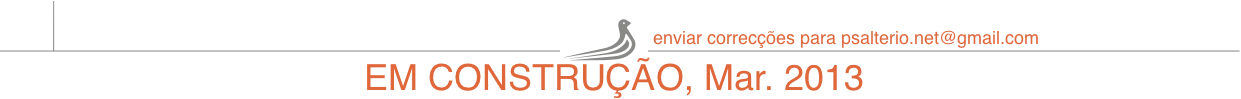
\includegraphics{_images/bkground_page_bottom.png}
}}





% this includes all the guitar tabs that may be needed
% must complete all the chords used in psalterio

% Cb chords

% C chords
\def \gtabCb{\gtab{Cb}{X32010:X32010}}
\def \gtabC{\gtab{C}{X32010:032010}}
\def \gtabCm{\gtab{Cm}{3:113321:004320}}

\def \gtabCsharpSusFour{\gtab{C\#sus4}{4:XX3341:XX2341}}

% Db chords

% D chords
\def \gtabD{\gtab{D}{X00232:000132}}
\def \gtabDm{\gtab{Dm}{X00231:000231}}
\def \gtabDfour{\gtab{D4}{X00233:000134}}
\def \gtabDseven{\gtab{D7}{X00212:000213}}
\def \gtabDsevenPlus{\gtab{D7+}{X00222:000111}}

% D#/Eb chords
\def \gtabDsharp{\gtab{D\#}{2:XX0232:000132}}

% E chords
\def \gtabE{\gtab{E}{022100:023100}}
\def \gtabEseven{\gtab{E}{020100:020100}}

\def \gtabEm{\gtab{Em}{022000:012000}}
\def \gtabEmSeven{\gtab{Em7}{022030:012040}}

% Gb chords

% F chords
\def \gtabF{\gtab{F}{1:133211:034200}}
\def \gtabFm{\gtab{Fm}{1:133111:034000}}


% F# chords
\def \gtabFsharpMinor{\gtab{F\#m}{2:133111:034000}}
\def \gtabFsharpMinorSeven{\gtab{F\#m7}{2:131131:030040}}

% Gb chords

% G chords
\def \gtabG{\gtab{G}{320033:210034}}
\def \gtabGseven{\gtab{G7}{320001:320001}}
\def \gtabGfret{\gtab{(G)}{3:133211:034200}}
\def \gtabGm{\gtab{Gm}{3:133111:034000}}


% G# / Ab chords

% A chords
\def \gtabA{\gtab{A}{X02220:001230}}
\def \gtabAm{\gtab{Am}{X02210:002310}}
\def \gtabAmSeven{\gtab{Am7}{X02010:002010}}
\def \gtabAfour{\gtab{A4}{X02230:001230}}
\def \gtabAseven{\gtab{A7}{X02020:001030}}

% Bb chords
\def \gtabBb{\gtab{Bb}{X13331}}

% B chords
\def \gtabB{\gtab{B}{X13331:003210}}
\def \gtabBm{\gtab{Bm}{X13321:003420}}
\def \gtabBmSeven{\gtab{Bm7}{X13121:003020}}



% after any { or } at the end of a line inside the macro definition add %, otherwise you'll get an extra space
\newcommand{\guitarTab}[1]{%
\ifstrequal{#1}{Cb}      {\gtab{Cb}{X32010:X32010}      }{}%
\ifstrequal{#1}{C}        { \gtab{C}{X32010:032010}       }{}%
%
%G
%
\ifstrequal{#1}{G}       { \gtab{G}{320033:210034}       }{}%
\ifstrequal{#1}{G7}     { \gtab{G7}{320001:320001}     }{}%
\ifstrequal{#1}{Gfret}  { \gtab{G}{3:133211:034200}    }{}%
\ifstrequal{#1}{Gm}    { \gtab{Gm}{3:133111:034000}  }{}%
} %end \newcommand{\gtab}

%muda aqui o numero da musica em que estas a trabalhar
%\def \selectSong{114}

\providebool{gchords}
\setbool{gchords}{true}

% set guitar chords vertical space separation with lyrics
\def \gchordsVspace{5 mm}

\begin{document}
	
	
	\AddToShipoutPicture*{\BottomPic}
	
	\begin{songs}{}
	
	%format file
	%
%Font Sizes
%
%\tiny
%\scriptsize
%\footnotesize
%\small
%\normalsize
%\large
%\Large
%\LARGE
%\huge
%\Huge


%\renewcommand{\thesongnum}{A\arabic{songnum}}
\renewcommand{\printsongnum}[1]{\sffamily\bfseries\huge\MakeUppercase#1}
\setlength{\songnumwidth}{2cm} % box width
%\renewcommand{\snumbgcolor}{white}

%change font for Title
\renewcommand{\stitlefont}{\sffamily\bfseries\huge\MakeUppercase} %song title

%remove verse numbers
%\noversenumbers 
% make left separation
\setlength{\versenumwidth}{2.0cm}

%verse separations
%\versesep=15pt
%\afterpreludeskip=2pt
%\beforepostludeskip=2pt
%\baselineadj=10pt

% separation between chords and lyrics
\renewcommand{\clineparams}{ 
\baselineskip=10pt 
%\lineskiplimit=2pt 
%\lineskip=5pt
}

% change font for lyrics
%\renewcommand{\lyricfont}{\sffamily}
%\renewcommand{\lyricfont}{\sffamily\small}
\renewcommand{\lyricfont}{\sffamily\large}
%\renewcommand{\chorusfont}{\sffamily}
\renewcommand{\chorusfont}{\sffamily\large}

%change the Chords formatting
\renewcommand{\printchord}[1]{\sffamily\color{red}\it\normalsize#1}

%check http://www.tug.org/pracjourn/2006-1/schmidt/schmidt.pdf


%\renewcommand{\songauthors}[1]{tete #1}


%\renewcommand{\extendpostlude}
%{ \songcopyright\ \songlicense\unskip \ Used with permission.}

\setlength{\cbarwidth}{0pt}
\setlength{\sbarheight}{0pt}

% music anf lyrics by
\newcommand{\musicLyricsBy}{} 
\newsongkey{mlby}{\def\musicLyricsBy{}}
                 {\def\musicLyricsBy{\sffamily\it\small letra e música por #1\par}}

% music anf lyrics by
\newcommand{\musicby}{} 
\newsongkey{music}{\def\musicby{}}
                 {\def\musicby{\sffamily\it\small música: #1\par}}

% music anf lyrics by
\newcommand{\lyricsby}{} 
\newsongkey{lyrics}{\def\lyricsby{}}
                 {\def\lyricsby{\sffamily\it\small letra: #1\par}}

%\renewcommand{\sharpsymbol}{\ensuremath{^\sharp}}
\renewcommand{\extendprelude}{
  \showrefs\showauthors 
  %{\bfseries\musicLyricsBy}
  {\bfseries\musicby}
  {\bfseries\lyricsby}
}

\def \gtabsOn{1}
	

%%%%%%%%%%%%%%%%%%%%%%%%%%%%%%%%%%%%%%%%%%%%%%%%%%%%%%%%%%%%%%%%%%%%%%%%%%%
% set song number
%%%%%%%%%%%%%%%%%%%%%%%%%%%%%%%%%%%%%%%%%%%%%%%%%%%%%%%%%%%%%%%%%%%%%%%%%%%
\setcounter{songnum}{19}

%%%%%%%%%%%%%%%%%%%%%%%%%%%%%%%%%%%%%%%%%%%%%%%%%%%%%%%%%%%%%%%%%%%%%%%%%%%
% begin song latex formating, set the title and other info
%%%%%%%%%%%%%%%%%%%%%%%%%%%%%%%%%%%%%%%%%%%%%%%%%%%%%%%%%%%%%%%%%%%%%%%%%%%
% song title
\beginsong{Em nada ponho a minha fé}[
        % music and lyric by
        % mlby={},
        % lyrics
        %lyrics={}, 
        % music by
        %music={},
        % bible verse
        %sr={},
        % licence/copyright
        %cr={Public domain.},
        % arrangement by
        %arr={},
        % index title
        index={Em nada ponho a minha fé}]

%%%%%%%%%%%%%%%%%%%%%%%%%%%%%%%%%%%%%%%%%%%%%%%%%%%%%%%%%%%%%%%%%%%%%%%%%%%
% section #1: verse 
%%%%%%%%%%%%%%%%%%%%%%%%%%%%%%%%%%%%%%%%%%%%%%%%%%%%%%%%%%%%%%%%%%%%%%%%%%%
\beginverse
\[F]Em nada ponho a mi\[C7]nha fé,
Se\[Bb]não na graça\[C7] de Je\[F]sus 
No sacrifício remi\[C7]dor,
No \[Bb]sangue do \[C7]bom Reden\[F]tor.
\endverse

%%%%%%%%%%%%%%%%%%%%%%%%%%%%%%%%%%%%%%%%%%%%%%%%%%%%%%%%%%%%%%%%%%%%%%%%%%%
% section #2: chorus 
%%%%%%%%%%%%%%%%%%%%%%%%%%%%%%%%%%%%%%%%%%%%%%%%%%%%%%%%%%%%%%%%%%%%%%%%%%%
\beginchorus
\[F]A minha fé e o\[Bb] meu amor
Es\[F]tão firmados no Se\[C7]nhor;
Es\[F]tão firmados \[C7]no Se\[F]nhor.
\endchorus

%%%%%%%%%%%%%%%%%%%%%%%%%%%%%%%%%%%%%%%%%%%%%%%%%%%%%%%%%%%%%%%%%%%%%%%%%%%
% section #3: verse 
%%%%%%%%%%%%%%%%%%%%%%%%%%%%%%%%%%%%%%%%%%%%%%%%%%%%%%%%%%%%%%%%%%%%%%%%%%%
\beginverse
Se Lhe não posso a face ver,
Na Sua graça vou viver. 
Em cada transe a suportar,
Sempre hei de n’Ele confiar.
\endverse

%%%%%%%%%%%%%%%%%%%%%%%%%%%%%%%%%%%%%%%%%%%%%%%%%%%%%%%%%%%%%%%%%%%%%%%%%%%
% section #4: verse 
%%%%%%%%%%%%%%%%%%%%%%%%%%%%%%%%%%%%%%%%%%%%%%%%%%%%%%%%%%%%%%%%%%%%%%%%%%%
\beginverse
Seu juramento é mui leal,
Abriga-me no temporal
Ao vir cercar-me a tentação,
É Cristo a minha salvação.
\endverse

%%%%%%%%%%%%%%%%%%%%%%%%%%%%%%%%%%%%%%%%%%%%%%%%%%%%%%%%%%%%%%%%%%%%%%%%%%%
% section #5: verse 
%%%%%%%%%%%%%%%%%%%%%%%%%%%%%%%%%%%%%%%%%%%%%%%%%%%%%%%%%%%%%%%%%%%%%%%%%%%
\beginverse
Quando o clarim aflim soar,
Irei com Ele me encontrar;
E gozarei da redenção,
Com todos que no céu estão.
\endverse


%%%%%%%%%%%%%%%%%%%%%%%%%%%%%%%%%%%%%%%%%%%%%%%%%%%%%%%%%%%%%%%%%%%%%%%%%%%
% print guitar tabs used in this song
%%%%%%%%%%%%%%%%%%%%%%%%%%%%%%%%%%%%%%%%%%%%%%%%%%%%%%%%%%%%%%%%%%%%%%%%%%%
% if the guitar chords are to be printed
\ifbool{gchords}{
% set a vertical space of 10 pt 
\vspace{\gchordsVspace}
} % end if

%%%%%%%%%%%%%%%%%%%%%%%%%%%%%%%%%%%%%%%%%%%%%%%%%%%%%%%%%%%%%%%%%%%%%%%%%%%
% end song latex formating
%%%%%%%%%%%%%%%%%%%%%%%%%%%%%%%%%%%%%%%%%%%%%%%%%%%%%%%%%%%%%%%%%%%%%%%%%%%
% end song
\endsong

%include song latex footer
%	 %lilypond-book --output=out --pdf  106single.tex
	 %\lilypondfile[]{E_101.ly}
	
\end{document}
	%%%%%%%%%%%%%%%%%%%%%%%%%%%%%%%%%%%%%%%%%%%%%%%%%%%%%%%%%%%%%%%%%%%%%%%%%%%
% this has all the necessary packages and formatting for the document
%%%%%%%%%%%%%%%%%%%%%%%%%%%%%%%%%%%%%%%%%%%%%%%%%%%%%%%%%%%%%%%%%%%%%%%%%%%
%\def \includeFolder{../_include}

% this has all the necessary packages and formatting for the document
\documentclass[10pt,a5paper]{article}

%define include folder
\def \includeFolder{_include}

%packages
\usepackage[left=1cm,right=1cm,top=1cm,bottom=1cm]{geometry}

\usepackage[chorded]{\includeFolder/psalterio} %must check the licence to change the name of the sty file!!!
%\usepackage[chorded]{resources/songs-old} %must check the licence to change the name of the sty file!!!

\usepackage[utf8]{inputenc}

\usepackage{graphicx}
\usepackage{wrapfig}
\usepackage{wallpaper}
\usepackage{color}
\usepackage{eso-pic} %for background pictures
\usepackage[bookmarks]{hyperref} 
%\usepackage{ifthen} %etoolbox is more up to date
\usepackage{etoolbox}


%\usepackage[xetex]{graphicx}
%\usepackage{fontspec,xunicode}
%\defaultfontfeatures{Mapping=tex-text,Scale=MatchLowercase}
%\setmainfont[Scale=.95]{Times}
%\setmonofont{Lucida Sans Typewriter}

%\usepackage[portuguese]{babel}
%\usepackage[latin1]{inputenc}
%\usepackage[utf8]{inputenc}
%\usepackage[T1]{fontenc}
%\usepackage[scaled]{uarial}
%\usepackage{helvet}
%\renewcommand{\familydefault}{\sfdefault}

%this removes the page number
\thispagestyle{empty}
\pagestyle{empty}
\songcolumns{1}

\parindent 0pt

%add background picture
\newcommand\BackgroundPic{
\put(0,0){
\parbox[b][\paperheight]{\paperwidth}{%
\vfill
\centering

\includegraphics[width=\paperwidth,height=\paperheight,
keepaspectratio]{logo.png}%
\vfill
}}}

\newcommand\BottomPic{
\put(0,0){
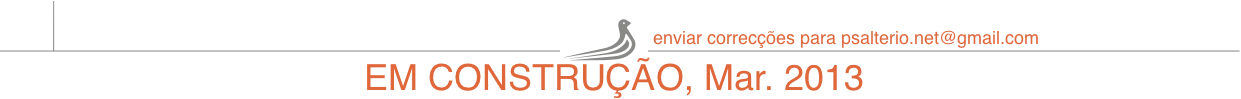
\includegraphics{_images/bkground_page_bottom.png}
}}





% this includes all the guitar tabs that may be needed
% must complete all the chords used in psalterio

% Cb chords

% C chords
\def \gtabCb{\gtab{Cb}{X32010:X32010}}
\def \gtabC{\gtab{C}{X32010:032010}}
\def \gtabCm{\gtab{Cm}{3:113321:004320}}

\def \gtabCsharpSusFour{\gtab{C\#sus4}{4:XX3341:XX2341}}

% Db chords

% D chords
\def \gtabD{\gtab{D}{X00232:000132}}
\def \gtabDm{\gtab{Dm}{X00231:000231}}
\def \gtabDfour{\gtab{D4}{X00233:000134}}
\def \gtabDseven{\gtab{D7}{X00212:000213}}
\def \gtabDsevenPlus{\gtab{D7+}{X00222:000111}}

% D#/Eb chords
\def \gtabDsharp{\gtab{D\#}{2:XX0232:000132}}

% E chords
\def \gtabE{\gtab{E}{022100:023100}}
\def \gtabEseven{\gtab{E}{020100:020100}}

\def \gtabEm{\gtab{Em}{022000:012000}}
\def \gtabEmSeven{\gtab{Em7}{022030:012040}}

% Gb chords

% F chords
\def \gtabF{\gtab{F}{1:133211:034200}}
\def \gtabFm{\gtab{Fm}{1:133111:034000}}


% F# chords
\def \gtabFsharpMinor{\gtab{F\#m}{2:133111:034000}}
\def \gtabFsharpMinorSeven{\gtab{F\#m7}{2:131131:030040}}

% Gb chords

% G chords
\def \gtabG{\gtab{G}{320033:210034}}
\def \gtabGseven{\gtab{G7}{320001:320001}}
\def \gtabGfret{\gtab{(G)}{3:133211:034200}}
\def \gtabGm{\gtab{Gm}{3:133111:034000}}


% G# / Ab chords

% A chords
\def \gtabA{\gtab{A}{X02220:001230}}
\def \gtabAm{\gtab{Am}{X02210:002310}}
\def \gtabAmSeven{\gtab{Am7}{X02010:002010}}
\def \gtabAfour{\gtab{A4}{X02230:001230}}
\def \gtabAseven{\gtab{A7}{X02020:001030}}

% Bb chords
\def \gtabBb{\gtab{Bb}{X13331}}

% B chords
\def \gtabB{\gtab{B}{X13331:003210}}
\def \gtabBm{\gtab{Bm}{X13321:003420}}
\def \gtabBmSeven{\gtab{Bm7}{X13121:003020}}



% after any { or } at the end of a line inside the macro definition add %, otherwise you'll get an extra space
\newcommand{\guitarTab}[1]{%
\ifstrequal{#1}{Cb}      {\gtab{Cb}{X32010:X32010}      }{}%
\ifstrequal{#1}{C}        { \gtab{C}{X32010:032010}       }{}%
%
%G
%
\ifstrequal{#1}{G}       { \gtab{G}{320033:210034}       }{}%
\ifstrequal{#1}{G7}     { \gtab{G7}{320001:320001}     }{}%
\ifstrequal{#1}{Gfret}  { \gtab{G}{3:133211:034200}    }{}%
\ifstrequal{#1}{Gm}    { \gtab{Gm}{3:133111:034000}  }{}%
} %end \newcommand{\gtab}

%muda aqui o numero da musica em que estas a trabalhar
%\def \selectSong{114}

\providebool{gchords}
\setbool{gchords}{true}

% set guitar chords vertical space separation with lyrics
\def \gchordsVspace{5 mm}

\begin{document}
	
	
	\AddToShipoutPicture*{\BottomPic}
	
	\begin{songs}{}
	
	%format file
	%
%Font Sizes
%
%\tiny
%\scriptsize
%\footnotesize
%\small
%\normalsize
%\large
%\Large
%\LARGE
%\huge
%\Huge


%\renewcommand{\thesongnum}{A\arabic{songnum}}
\renewcommand{\printsongnum}[1]{\sffamily\bfseries\huge\MakeUppercase#1}
\setlength{\songnumwidth}{2cm} % box width
%\renewcommand{\snumbgcolor}{white}

%change font for Title
\renewcommand{\stitlefont}{\sffamily\bfseries\huge\MakeUppercase} %song title

%remove verse numbers
%\noversenumbers 
% make left separation
\setlength{\versenumwidth}{2.0cm}

%verse separations
%\versesep=15pt
%\afterpreludeskip=2pt
%\beforepostludeskip=2pt
%\baselineadj=10pt

% separation between chords and lyrics
\renewcommand{\clineparams}{ 
\baselineskip=10pt 
%\lineskiplimit=2pt 
%\lineskip=5pt
}

% change font for lyrics
%\renewcommand{\lyricfont}{\sffamily}
%\renewcommand{\lyricfont}{\sffamily\small}
\renewcommand{\lyricfont}{\sffamily\large}
%\renewcommand{\chorusfont}{\sffamily}
\renewcommand{\chorusfont}{\sffamily\large}

%change the Chords formatting
\renewcommand{\printchord}[1]{\sffamily\color{red}\it\normalsize#1}

%check http://www.tug.org/pracjourn/2006-1/schmidt/schmidt.pdf


%\renewcommand{\songauthors}[1]{tete #1}


%\renewcommand{\extendpostlude}
%{ \songcopyright\ \songlicense\unskip \ Used with permission.}

\setlength{\cbarwidth}{0pt}
\setlength{\sbarheight}{0pt}

% music anf lyrics by
\newcommand{\musicLyricsBy}{} 
\newsongkey{mlby}{\def\musicLyricsBy{}}
                 {\def\musicLyricsBy{\sffamily\it\small letra e música por #1\par}}

% music anf lyrics by
\newcommand{\musicby}{} 
\newsongkey{music}{\def\musicby{}}
                 {\def\musicby{\sffamily\it\small música: #1\par}}

% music anf lyrics by
\newcommand{\lyricsby}{} 
\newsongkey{lyrics}{\def\lyricsby{}}
                 {\def\lyricsby{\sffamily\it\small letra: #1\par}}

%\renewcommand{\sharpsymbol}{\ensuremath{^\sharp}}
\renewcommand{\extendprelude}{
  \showrefs\showauthors 
  %{\bfseries\musicLyricsBy}
  {\bfseries\musicby}
  {\bfseries\lyricsby}
}

\def \gtabsOn{1}
	

%%%%%%%%%%%%%%%%%%%%%%%%%%%%%%%%%%%%%%%%%%%%%%%%%%%%%%%%%%%%%%%%%%%%%%%%%%%
% set song number
%%%%%%%%%%%%%%%%%%%%%%%%%%%%%%%%%%%%%%%%%%%%%%%%%%%%%%%%%%%%%%%%%%%%%%%%%%%
\setcounter{songnum}{20}

%%%%%%%%%%%%%%%%%%%%%%%%%%%%%%%%%%%%%%%%%%%%%%%%%%%%%%%%%%%%%%%%%%%%%%%%%%%
% begin song latex formating, set the title and other info
%%%%%%%%%%%%%%%%%%%%%%%%%%%%%%%%%%%%%%%%%%%%%%%%%%%%%%%%%%%%%%%%%%%%%%%%%%%
% song title
\beginsong{Estranha graça de Jesus}[
        % music and lyric by
        % mlby={},
        % lyrics
        %lyrics={}, 
        % music by
        %music={},
        % bible verse
        %sr={},
        % licence/copyright
        %cr={Public domain.},
        % arrangement by
        %arr={},
        % index title
        index={Estranha graça de Jesus}]

%%%%%%%%%%%%%%%%%%%%%%%%%%%%%%%%%%%%%%%%%%%%%%%%%%%%%%%%%%%%%%%%%%%%%%%%%%%
% section #1: verse 
%%%%%%%%%%%%%%%%%%%%%%%%%%%%%%%%%%%%%%%%%%%%%%%%%%%%%%%%%%%%%%%%%%%%%%%%%%%
\beginverse
A es\[G]tranha \[D7]graça\[Em] de  \[C]Je\[G]sus
Um infe\[D7]liz sal\[G]vou!
Eu cego estava, \[C]deu-me \[G]luz
Per\[Em]dido e \[G]me \[D7]bus\[G]cou!
\endverse

%%%%%%%%%%%%%%%%%%%%%%%%%%%%%%%%%%%%%%%%%%%%%%%%%%%%%%%%%%%%%%%%%%%%%%%%%%%
% section #2: verse 
%%%%%%%%%%%%%%%%%%%%%%%%%%%%%%%%%%%%%%%%%%%%%%%%%%%%%%%%%%%%%%%%%%%%%%%%%%%
\beginverse
A graça então, meu coração,
Do medo libertou;
Oh! Quão preciosa a salvação
Que a graça me ganhou!
\endverse

%%%%%%%%%%%%%%%%%%%%%%%%%%%%%%%%%%%%%%%%%%%%%%%%%%%%%%%%%%%%%%%%%%%%%%%%%%%
% section #3: verse 
%%%%%%%%%%%%%%%%%%%%%%%%%%%%%%%%%%%%%%%%%%%%%%%%%%%%%%%%%%%%%%%%%%%%%%%%%%%
\beginverse
Perigos mil atravessei
E a graça me valeu;
Eu são e salvo agora irei
Ao santo lar do céu.
\endverse

%%%%%%%%%%%%%%%%%%%%%%%%%%%%%%%%%%%%%%%%%%%%%%%%%%%%%%%%%%%%%%%%%%%%%%%%%%%
% section #4: verse 
%%%%%%%%%%%%%%%%%%%%%%%%%%%%%%%%%%%%%%%%%%%%%%%%%%%%%%%%%%%%%%%%%%%%%%%%%%%
\beginverse
Promessas deu-me o Salvador,
E n’Ele eu posso crer,
É meu escudo e protector
Em todo meu viver!
\endverse


%%%%%%%%%%%%%%%%%%%%%%%%%%%%%%%%%%%%%%%%%%%%%%%%%%%%%%%%%%%%%%%%%%%%%%%%%%%
% print guitar tabs used in this song
%%%%%%%%%%%%%%%%%%%%%%%%%%%%%%%%%%%%%%%%%%%%%%%%%%%%%%%%%%%%%%%%%%%%%%%%%%%
% if the guitar chords are to be printed
\ifbool{gchords}{
% set a vertical space of 10 pt 
\vspace{\gchordsVspace}
} % end if

%%%%%%%%%%%%%%%%%%%%%%%%%%%%%%%%%%%%%%%%%%%%%%%%%%%%%%%%%%%%%%%%%%%%%%%%%%%
% end song latex formating
%%%%%%%%%%%%%%%%%%%%%%%%%%%%%%%%%%%%%%%%%%%%%%%%%%%%%%%%%%%%%%%%%%%%%%%%%%%
% end song
\endsong

%include song latex footer
%	 %lilypond-book --output=out --pdf  106single.tex
	 %\lilypondfile[]{E_101.ly}
	
\end{document}
	%%%%%%%%%%%%%%%%%%%%%%%%%%%%%%%%%%%%%%%%%%%%%%%%%%%%%%%%%%%%%%%%%%%%%%%%%%%
% this has all the necessary packages and formatting for the document
%%%%%%%%%%%%%%%%%%%%%%%%%%%%%%%%%%%%%%%%%%%%%%%%%%%%%%%%%%%%%%%%%%%%%%%%%%%
%\def \includeFolder{../_include}

% this has all the necessary packages and formatting for the document
\documentclass[10pt,a5paper]{article}

%define include folder
\def \includeFolder{_include}

%packages
\usepackage[left=1cm,right=1cm,top=1cm,bottom=1cm]{geometry}

\usepackage[chorded]{\includeFolder/psalterio} %must check the licence to change the name of the sty file!!!
%\usepackage[chorded]{resources/songs-old} %must check the licence to change the name of the sty file!!!

\usepackage[utf8]{inputenc}

\usepackage{graphicx}
\usepackage{wrapfig}
\usepackage{wallpaper}
\usepackage{color}
\usepackage{eso-pic} %for background pictures
\usepackage[bookmarks]{hyperref} 
%\usepackage{ifthen} %etoolbox is more up to date
\usepackage{etoolbox}


%\usepackage[xetex]{graphicx}
%\usepackage{fontspec,xunicode}
%\defaultfontfeatures{Mapping=tex-text,Scale=MatchLowercase}
%\setmainfont[Scale=.95]{Times}
%\setmonofont{Lucida Sans Typewriter}

%\usepackage[portuguese]{babel}
%\usepackage[latin1]{inputenc}
%\usepackage[utf8]{inputenc}
%\usepackage[T1]{fontenc}
%\usepackage[scaled]{uarial}
%\usepackage{helvet}
%\renewcommand{\familydefault}{\sfdefault}

%this removes the page number
\thispagestyle{empty}
\pagestyle{empty}
\songcolumns{1}

\parindent 0pt

%add background picture
\newcommand\BackgroundPic{
\put(0,0){
\parbox[b][\paperheight]{\paperwidth}{%
\vfill
\centering

\includegraphics[width=\paperwidth,height=\paperheight,
keepaspectratio]{logo.png}%
\vfill
}}}

\newcommand\BottomPic{
\put(0,0){
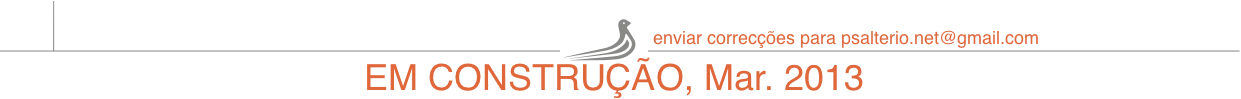
\includegraphics{_images/bkground_page_bottom.png}
}}





% this includes all the guitar tabs that may be needed
% must complete all the chords used in psalterio

% Cb chords

% C chords
\def \gtabCb{\gtab{Cb}{X32010:X32010}}
\def \gtabC{\gtab{C}{X32010:032010}}
\def \gtabCm{\gtab{Cm}{3:113321:004320}}

\def \gtabCsharpSusFour{\gtab{C\#sus4}{4:XX3341:XX2341}}

% Db chords

% D chords
\def \gtabD{\gtab{D}{X00232:000132}}
\def \gtabDm{\gtab{Dm}{X00231:000231}}
\def \gtabDfour{\gtab{D4}{X00233:000134}}
\def \gtabDseven{\gtab{D7}{X00212:000213}}
\def \gtabDsevenPlus{\gtab{D7+}{X00222:000111}}

% D#/Eb chords
\def \gtabDsharp{\gtab{D\#}{2:XX0232:000132}}

% E chords
\def \gtabE{\gtab{E}{022100:023100}}
\def \gtabEseven{\gtab{E}{020100:020100}}

\def \gtabEm{\gtab{Em}{022000:012000}}
\def \gtabEmSeven{\gtab{Em7}{022030:012040}}

% Gb chords

% F chords
\def \gtabF{\gtab{F}{1:133211:034200}}
\def \gtabFm{\gtab{Fm}{1:133111:034000}}


% F# chords
\def \gtabFsharpMinor{\gtab{F\#m}{2:133111:034000}}
\def \gtabFsharpMinorSeven{\gtab{F\#m7}{2:131131:030040}}

% Gb chords

% G chords
\def \gtabG{\gtab{G}{320033:210034}}
\def \gtabGseven{\gtab{G7}{320001:320001}}
\def \gtabGfret{\gtab{(G)}{3:133211:034200}}
\def \gtabGm{\gtab{Gm}{3:133111:034000}}


% G# / Ab chords

% A chords
\def \gtabA{\gtab{A}{X02220:001230}}
\def \gtabAm{\gtab{Am}{X02210:002310}}
\def \gtabAmSeven{\gtab{Am7}{X02010:002010}}
\def \gtabAfour{\gtab{A4}{X02230:001230}}
\def \gtabAseven{\gtab{A7}{X02020:001030}}

% Bb chords
\def \gtabBb{\gtab{Bb}{X13331}}

% B chords
\def \gtabB{\gtab{B}{X13331:003210}}
\def \gtabBm{\gtab{Bm}{X13321:003420}}
\def \gtabBmSeven{\gtab{Bm7}{X13121:003020}}



% after any { or } at the end of a line inside the macro definition add %, otherwise you'll get an extra space
\newcommand{\guitarTab}[1]{%
\ifstrequal{#1}{Cb}      {\gtab{Cb}{X32010:X32010}      }{}%
\ifstrequal{#1}{C}        { \gtab{C}{X32010:032010}       }{}%
%
%G
%
\ifstrequal{#1}{G}       { \gtab{G}{320033:210034}       }{}%
\ifstrequal{#1}{G7}     { \gtab{G7}{320001:320001}     }{}%
\ifstrequal{#1}{Gfret}  { \gtab{G}{3:133211:034200}    }{}%
\ifstrequal{#1}{Gm}    { \gtab{Gm}{3:133111:034000}  }{}%
} %end \newcommand{\gtab}

%muda aqui o numero da musica em que estas a trabalhar
%\def \selectSong{114}

\providebool{gchords}
\setbool{gchords}{true}

% set guitar chords vertical space separation with lyrics
\def \gchordsVspace{5 mm}

\begin{document}
	
	
	\AddToShipoutPicture*{\BottomPic}
	
	\begin{songs}{}
	
	%format file
	%
%Font Sizes
%
%\tiny
%\scriptsize
%\footnotesize
%\small
%\normalsize
%\large
%\Large
%\LARGE
%\huge
%\Huge


%\renewcommand{\thesongnum}{A\arabic{songnum}}
\renewcommand{\printsongnum}[1]{\sffamily\bfseries\huge\MakeUppercase#1}
\setlength{\songnumwidth}{2cm} % box width
%\renewcommand{\snumbgcolor}{white}

%change font for Title
\renewcommand{\stitlefont}{\sffamily\bfseries\huge\MakeUppercase} %song title

%remove verse numbers
%\noversenumbers 
% make left separation
\setlength{\versenumwidth}{2.0cm}

%verse separations
%\versesep=15pt
%\afterpreludeskip=2pt
%\beforepostludeskip=2pt
%\baselineadj=10pt

% separation between chords and lyrics
\renewcommand{\clineparams}{ 
\baselineskip=10pt 
%\lineskiplimit=2pt 
%\lineskip=5pt
}

% change font for lyrics
%\renewcommand{\lyricfont}{\sffamily}
%\renewcommand{\lyricfont}{\sffamily\small}
\renewcommand{\lyricfont}{\sffamily\large}
%\renewcommand{\chorusfont}{\sffamily}
\renewcommand{\chorusfont}{\sffamily\large}

%change the Chords formatting
\renewcommand{\printchord}[1]{\sffamily\color{red}\it\normalsize#1}

%check http://www.tug.org/pracjourn/2006-1/schmidt/schmidt.pdf


%\renewcommand{\songauthors}[1]{tete #1}


%\renewcommand{\extendpostlude}
%{ \songcopyright\ \songlicense\unskip \ Used with permission.}

\setlength{\cbarwidth}{0pt}
\setlength{\sbarheight}{0pt}

% music anf lyrics by
\newcommand{\musicLyricsBy}{} 
\newsongkey{mlby}{\def\musicLyricsBy{}}
                 {\def\musicLyricsBy{\sffamily\it\small letra e música por #1\par}}

% music anf lyrics by
\newcommand{\musicby}{} 
\newsongkey{music}{\def\musicby{}}
                 {\def\musicby{\sffamily\it\small música: #1\par}}

% music anf lyrics by
\newcommand{\lyricsby}{} 
\newsongkey{lyrics}{\def\lyricsby{}}
                 {\def\lyricsby{\sffamily\it\small letra: #1\par}}

%\renewcommand{\sharpsymbol}{\ensuremath{^\sharp}}
\renewcommand{\extendprelude}{
  \showrefs\showauthors 
  %{\bfseries\musicLyricsBy}
  {\bfseries\musicby}
  {\bfseries\lyricsby}
}

\def \gtabsOn{1}
	

%%%%%%%%%%%%%%%%%%%%%%%%%%%%%%%%%%%%%%%%%%%%%%%%%%%%%%%%%%%%%%%%%%%%%%%%%%%
% set song number
%%%%%%%%%%%%%%%%%%%%%%%%%%%%%%%%%%%%%%%%%%%%%%%%%%%%%%%%%%%%%%%%%%%%%%%%%%%
\setcounter{songnum}{21}

%%%%%%%%%%%%%%%%%%%%%%%%%%%%%%%%%%%%%%%%%%%%%%%%%%%%%%%%%%%%%%%%%%%%%%%%%%%
% begin song latex formating, set the title and other info
%%%%%%%%%%%%%%%%%%%%%%%%%%%%%%%%%%%%%%%%%%%%%%%%%%%%%%%%%%%%%%%%%%%%%%%%%%%
% song title
\beginsong{Amen}[
%%% music and lyric by
% mlby={},
%%% lyrics
%lyrics={}, 
%%% music by
%music={},
%%% bible verse
%sr={},
%%% licence/copyright
%cr={Public domain.},
%%% arrangement by
%arr={},
%%% index title
index={Amen}]

%%%%%%%%%%%%%%%%%%%%%%%%%%%%%%%%%%%%%%%%%%%%%%%%%%%%%%%%%%%%%%%%%%%%%%%%%%%
% section #1: verse 
%%%%%%%%%%%%%%%%%%%%%%%%%%%%%%%%%%%%%%%%%%%%%%%%%%%%%%%%%%%%%%%%%%%%%%%%%%%
\beginverse
S\[F]ee \[C7]the ba\[F]by,
Lying in a \[C7]man\[F]ger
\endverse

%%%%%%%%%%%%%%%%%%%%%%%%%%%%%%%%%%%%%%%%%%%%%%%%%%%%%%%%%%%%%%%%%%%%%%%%%%%
% section #2: chorus 
%%%%%%%%%%%%%%%%%%%%%%%%%%%%%%%%%%%%%%%%%%%%%%%%%%%%%%%%%%%%%%%%%%%%%%%%%%%
\beginchorus
A\[F]men, Amen, Amen, \[Gm]Am\[F]en\[C7], Am\[F]en.
Hal\[Bb]leluja\[Dm]h, \[F]in t\[C7]he \[Dm Bb F]kingdom
Wi\[Bb]th my Sa\[F]vior. \[Bb F]Amen, \[C F]Amen.
\endchorus

\chordsoff
%%%%%%%%%%%%%%%%%%%%%%%%%%%%%%%%%%%%%%%%%%%%%%%%%%%%%%%%%%%%%%%%%%%%%%%%%%%
% section #3: verse 
%%%%%%%%%%%%%%%%%%%%%%%%%%%%%%%%%%%%%%%%%%%%%%%%%%%%%%%%%%%%%%%%%%%%%%%%%%%
\beginverse
See Him in the temple, Talking to the elders,
How they marveled at His wisdom!
\endverse

%%%%%%%%%%%%%%%%%%%%%%%%%%%%%%%%%%%%%%%%%%%%%%%%%%%%%%%%%%%%%%%%%%%%%%%%%%%
% section #4: verse 
%%%%%%%%%%%%%%%%%%%%%%%%%%%%%%%%%%%%%%%%%%%%%%%%%%%%%%%%%%%%%%%%%%%%%%%%%%%
\beginverse
See Him at the sea side, Preaching and healing,
To the blind and the feeble.
\endverse

%%%%%%%%%%%%%%%%%%%%%%%%%%%%%%%%%%%%%%%%%%%%%%%%%%%%%%%%%%%%%%%%%%%%%%%%%%%
% section #5: verse 
%%%%%%%%%%%%%%%%%%%%%%%%%%%%%%%%%%%%%%%%%%%%%%%%%%%%%%%%%%%%%%%%%%%%%%%%%%%
\beginverse
See Him in the garden, Praying to His Father,
In the deepest sorrow.
\endverse

%%%%%%%%%%%%%%%%%%%%%%%%%%%%%%%%%%%%%%%%%%%%%%%%%%%%%%%%%%%%%%%%%%%%%%%%%%%
% section #6: verse 
%%%%%%%%%%%%%%%%%%%%%%%%%%%%%%%%%%%%%%%%%%%%%%%%%%%%%%%%%%%%%%%%%%%%%%%%%%%
\beginverse
Yes, He is my Savior, Jesus died to save us,
And He rose on Easter.
\endverse


%%%%%%%%%%%%%%%%%%%%%%%%%%%%%%%%%%%%%%%%%%%%%%%%%%%%%%%%%%%%%%%%%%%%%%%%%%%
% print guitar tabs used in this song
%%%%%%%%%%%%%%%%%%%%%%%%%%%%%%%%%%%%%%%%%%%%%%%%%%%%%%%%%%%%%%%%%%%%%%%%%%%
% if the guitar chords are to be printed
\ifbool{gchords}{
% set a vertical space of 10 pt 
\vspace{\gchordsVspace}
} % end if

%%%%%%%%%%%%%%%%%%%%%%%%%%%%%%%%%%%%%%%%%%%%%%%%%%%%%%%%%%%%%%%%%%%%%%%%%%%
% end song latex formating
%%%%%%%%%%%%%%%%%%%%%%%%%%%%%%%%%%%%%%%%%%%%%%%%%%%%%%%%%%%%%%%%%%%%%%%%%%%
% end song
\endsong

%include song latex footer
%	 %lilypond-book --output=out --pdf  106single.tex
	 %\lilypondfile[]{E_101.ly}
	
\end{document}
	%%%%%%%%%%%%%%%%%%%%%%%%%%%%%%%%%%%%%%%%%%%%%%%%%%%%%%%%%%%%%%%%%%%%%%%%%%%
% this has all the necessary packages and formatting for the document
%%%%%%%%%%%%%%%%%%%%%%%%%%%%%%%%%%%%%%%%%%%%%%%%%%%%%%%%%%%%%%%%%%%%%%%%%%%
%\def \includeFolder{../_include}

% this has all the necessary packages and formatting for the document
\documentclass[10pt,a5paper]{article}

%define include folder
\def \includeFolder{_include}

%packages
\usepackage[left=1cm,right=1cm,top=1cm,bottom=1cm]{geometry}

\usepackage[chorded]{\includeFolder/psalterio} %must check the licence to change the name of the sty file!!!
%\usepackage[chorded]{resources/songs-old} %must check the licence to change the name of the sty file!!!

\usepackage[utf8]{inputenc}

\usepackage{graphicx}
\usepackage{wrapfig}
\usepackage{wallpaper}
\usepackage{color}
\usepackage{eso-pic} %for background pictures
\usepackage[bookmarks]{hyperref} 
%\usepackage{ifthen} %etoolbox is more up to date
\usepackage{etoolbox}


%\usepackage[xetex]{graphicx}
%\usepackage{fontspec,xunicode}
%\defaultfontfeatures{Mapping=tex-text,Scale=MatchLowercase}
%\setmainfont[Scale=.95]{Times}
%\setmonofont{Lucida Sans Typewriter}

%\usepackage[portuguese]{babel}
%\usepackage[latin1]{inputenc}
%\usepackage[utf8]{inputenc}
%\usepackage[T1]{fontenc}
%\usepackage[scaled]{uarial}
%\usepackage{helvet}
%\renewcommand{\familydefault}{\sfdefault}

%this removes the page number
\thispagestyle{empty}
\pagestyle{empty}
\songcolumns{1}

\parindent 0pt

%add background picture
\newcommand\BackgroundPic{
\put(0,0){
\parbox[b][\paperheight]{\paperwidth}{%
\vfill
\centering

\includegraphics[width=\paperwidth,height=\paperheight,
keepaspectratio]{logo.png}%
\vfill
}}}

\newcommand\BottomPic{
\put(0,0){
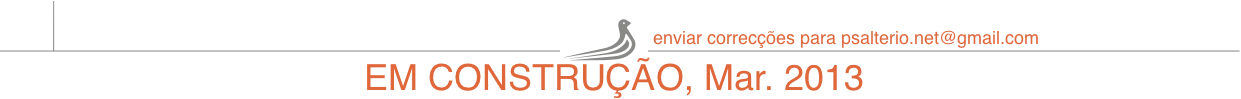
\includegraphics{_images/bkground_page_bottom.png}
}}





% this includes all the guitar tabs that may be needed
% must complete all the chords used in psalterio

% Cb chords

% C chords
\def \gtabCb{\gtab{Cb}{X32010:X32010}}
\def \gtabC{\gtab{C}{X32010:032010}}
\def \gtabCm{\gtab{Cm}{3:113321:004320}}

\def \gtabCsharpSusFour{\gtab{C\#sus4}{4:XX3341:XX2341}}

% Db chords

% D chords
\def \gtabD{\gtab{D}{X00232:000132}}
\def \gtabDm{\gtab{Dm}{X00231:000231}}
\def \gtabDfour{\gtab{D4}{X00233:000134}}
\def \gtabDseven{\gtab{D7}{X00212:000213}}
\def \gtabDsevenPlus{\gtab{D7+}{X00222:000111}}

% D#/Eb chords
\def \gtabDsharp{\gtab{D\#}{2:XX0232:000132}}

% E chords
\def \gtabE{\gtab{E}{022100:023100}}
\def \gtabEseven{\gtab{E}{020100:020100}}

\def \gtabEm{\gtab{Em}{022000:012000}}
\def \gtabEmSeven{\gtab{Em7}{022030:012040}}

% Gb chords

% F chords
\def \gtabF{\gtab{F}{1:133211:034200}}
\def \gtabFm{\gtab{Fm}{1:133111:034000}}


% F# chords
\def \gtabFsharpMinor{\gtab{F\#m}{2:133111:034000}}
\def \gtabFsharpMinorSeven{\gtab{F\#m7}{2:131131:030040}}

% Gb chords

% G chords
\def \gtabG{\gtab{G}{320033:210034}}
\def \gtabGseven{\gtab{G7}{320001:320001}}
\def \gtabGfret{\gtab{(G)}{3:133211:034200}}
\def \gtabGm{\gtab{Gm}{3:133111:034000}}


% G# / Ab chords

% A chords
\def \gtabA{\gtab{A}{X02220:001230}}
\def \gtabAm{\gtab{Am}{X02210:002310}}
\def \gtabAmSeven{\gtab{Am7}{X02010:002010}}
\def \gtabAfour{\gtab{A4}{X02230:001230}}
\def \gtabAseven{\gtab{A7}{X02020:001030}}

% Bb chords
\def \gtabBb{\gtab{Bb}{X13331}}

% B chords
\def \gtabB{\gtab{B}{X13331:003210}}
\def \gtabBm{\gtab{Bm}{X13321:003420}}
\def \gtabBmSeven{\gtab{Bm7}{X13121:003020}}



% after any { or } at the end of a line inside the macro definition add %, otherwise you'll get an extra space
\newcommand{\guitarTab}[1]{%
\ifstrequal{#1}{Cb}      {\gtab{Cb}{X32010:X32010}      }{}%
\ifstrequal{#1}{C}        { \gtab{C}{X32010:032010}       }{}%
%
%G
%
\ifstrequal{#1}{G}       { \gtab{G}{320033:210034}       }{}%
\ifstrequal{#1}{G7}     { \gtab{G7}{320001:320001}     }{}%
\ifstrequal{#1}{Gfret}  { \gtab{G}{3:133211:034200}    }{}%
\ifstrequal{#1}{Gm}    { \gtab{Gm}{3:133111:034000}  }{}%
} %end \newcommand{\gtab}

%muda aqui o numero da musica em que estas a trabalhar
%\def \selectSong{114}

\providebool{gchords}
\setbool{gchords}{true}

% set guitar chords vertical space separation with lyrics
\def \gchordsVspace{5 mm}

\begin{document}
	
	
	\AddToShipoutPicture*{\BottomPic}
	
	\begin{songs}{}
	
	%format file
	%
%Font Sizes
%
%\tiny
%\scriptsize
%\footnotesize
%\small
%\normalsize
%\large
%\Large
%\LARGE
%\huge
%\Huge


%\renewcommand{\thesongnum}{A\arabic{songnum}}
\renewcommand{\printsongnum}[1]{\sffamily\bfseries\huge\MakeUppercase#1}
\setlength{\songnumwidth}{2cm} % box width
%\renewcommand{\snumbgcolor}{white}

%change font for Title
\renewcommand{\stitlefont}{\sffamily\bfseries\huge\MakeUppercase} %song title

%remove verse numbers
%\noversenumbers 
% make left separation
\setlength{\versenumwidth}{2.0cm}

%verse separations
%\versesep=15pt
%\afterpreludeskip=2pt
%\beforepostludeskip=2pt
%\baselineadj=10pt

% separation between chords and lyrics
\renewcommand{\clineparams}{ 
\baselineskip=10pt 
%\lineskiplimit=2pt 
%\lineskip=5pt
}

% change font for lyrics
%\renewcommand{\lyricfont}{\sffamily}
%\renewcommand{\lyricfont}{\sffamily\small}
\renewcommand{\lyricfont}{\sffamily\large}
%\renewcommand{\chorusfont}{\sffamily}
\renewcommand{\chorusfont}{\sffamily\large}

%change the Chords formatting
\renewcommand{\printchord}[1]{\sffamily\color{red}\it\normalsize#1}

%check http://www.tug.org/pracjourn/2006-1/schmidt/schmidt.pdf


%\renewcommand{\songauthors}[1]{tete #1}


%\renewcommand{\extendpostlude}
%{ \songcopyright\ \songlicense\unskip \ Used with permission.}

\setlength{\cbarwidth}{0pt}
\setlength{\sbarheight}{0pt}

% music anf lyrics by
\newcommand{\musicLyricsBy}{} 
\newsongkey{mlby}{\def\musicLyricsBy{}}
                 {\def\musicLyricsBy{\sffamily\it\small letra e música por #1\par}}

% music anf lyrics by
\newcommand{\musicby}{} 
\newsongkey{music}{\def\musicby{}}
                 {\def\musicby{\sffamily\it\small música: #1\par}}

% music anf lyrics by
\newcommand{\lyricsby}{} 
\newsongkey{lyrics}{\def\lyricsby{}}
                 {\def\lyricsby{\sffamily\it\small letra: #1\par}}

%\renewcommand{\sharpsymbol}{\ensuremath{^\sharp}}
\renewcommand{\extendprelude}{
  \showrefs\showauthors 
  %{\bfseries\musicLyricsBy}
  {\bfseries\musicby}
  {\bfseries\lyricsby}
}

\def \gtabsOn{1}
	

%%%%%%%%%%%%%%%%%%%%%%%%%%%%%%%%%%%%%%%%%%%%%%%%%%%%%%%%%%%%%%%%%%%%%%%%%%%
% set song number
%%%%%%%%%%%%%%%%%%%%%%%%%%%%%%%%%%%%%%%%%%%%%%%%%%%%%%%%%%%%%%%%%%%%%%%%%%%
\setcounter{songnum}{22}						% song number

%%%%%%%%%%%%%%%%%%%%%%%%%%%%%%%%%%%%%%%%%%%%%%%%%%%%%%%%%%%%%%%%%%%%%%%%%%%
% begin song latex formating, set the title and other info
%%%%%%%%%%%%%%%%%%%%%%%%%%%%%%%%%%%%%%%%%%%%%%%%%%%%%%%%%%%%%%%%%%%%%%%%%%%
\beginsong{Sal da Terra}[					% song title ...
mlby={},								% music and lyric by
%lyrics={},					% music and lyric by
%music={},						% music and lyric by
%sr={},									% bible verse
%cr={Public domain.},         			% licence
%arr={my},                    			% arrangement by
index={Sal da Terra}]					% index title ...	
%%%%%%%%%%%%%%%%%%%%%%%%%%%%%%%%%%%%%%%%%%%%%%%%%%%%%%%%%%%%%%%%%%%%%%%%%%%
% verse #1
%%%%%%%%%%%%%%%%%%%%%%%%%%%%%%%%%%%%%%%%%%%%%%%%%%%%%%%%%%%%%%%%%%%%%%%%%%%
\beginverse										% start verse
Vós \[Bm]sois o \[A7]sal da \[D]terra, vós \[Bm]sois a \[A7]luz do \[D]mundo.
Ninguém mais \[A7]quer o \[D]sal, quan\[A7]do ele \[D]perde \[A7]o seu sabor.
\[D]Ninguém \[A7]acende a \[D]luz, para \[A7]escon\[D]dê-la \[A7]logo após.
\[D]O sal e a luz sou \[G]eu! Eu \[A7]sou do povo do \[D]Senhor.
\endverse										% end verse
%%%%%%%%%%%%%%%%%%%%%%%%%%%%%%%%%%%%%%%%%%%%%%%%%%%%%%%%%%%%%%%%%%%%%%%%%%%
% chorus #1
%%%%%%%%%%%%%%%%%%%%%%%%%%%%%%%%%%%%%%%%%%%%%%%%%%%%%%%%%%%%%%%%%%%%%%%%%%%
\beginchorus									% start chorus
\chordsoff
Eu quero que esta vida tenha muito mais sabor.
Eu quero que meu povo tenha muito mais amor.
Ninguém acende a luz para escondê-la logo após.
O sal e a luz sou eu! Eu sou do povo do Senhor.
\chordson
\endchorus										% end chorus
%%%%%%%%%%%%%%%%%%%%%%%%%%%%%%%%%%%%%%%%%%%%%%%%%%%%%%%%%%%%%%%%%%%%%%%%%%%
% verse #2
%%%%%%%%%%%%%%%%%%%%%%%%%%%%%%%%%%%%%%%%%%%%%%%%%%%%%%%%%%%%%%%%%%%%%%%%%%%
\beginverse										% start verse
\chordsoff
Vós sois o sal da terra! Vós sois a luz do mundo!
Há muito prato insípido, no mundo sem sabor.
Há muita escuridão, cegando o mundo sem amor.
O sal e a luz sou eu! Eu sou do povo do Senhor.
\chordson
\endverse										% end verse
%%%%%%%%%%%%%%%%%%%%%%%%%%%%%%%%%%%%%%%%%%%%%%%%%%%%%%%%%%%%%%%%%%%%%%%%%%%
% verse #3
%%%%%%%%%%%%%%%%%%%%%%%%%%%%%%%%%%%%%%%%%%%%%%%%%%%%%%%%%%%%%%%%%%%%%%%%%%%
\beginverse										% start verse
\chordsoff
Há vidas sem tempero, muita gente sofre a dor.
Existe escuridão, cegando o mundo sem amor.
Ninguém acende a luz para escondê-la logo após.
O sal e a luz sou eu! Eu sou do povo do Senhor

Vós sois o sal da terra! Vós sois a luz do mundo!
Num mundo que não ama, é preciso ter amor.
“Amai-vos uns aos outros”, é o desejo do Senhor.
O sal e a luz sou eu! Eu sou do povo do Senhor. (repete)
\chordson
\endverse										% end verse
%%%%%%%%%%%%%%%%%%%%%%%%%%%%%%%%%%%%%%%%%%%%%%%%%%%%%%%%%%%%%%%%%%%%%%%%%%%
% print guitar tabs used in this song
%%%%%%%%%%%%%%%%%%%%%%%%%%%%%%%%%%%%%%%%%%%%%%%%%%%%%%%%%%%%%%%%%%%%%%%%%%%
\ifbool{gchords}{					% if the guitar chords are to be printed
space{\gchordsVspace}				% set a vertical space of 10 pt 

}									% end if

%%%%%%%%%%%%%%%%%%%%%%%%%%%%%%%%%%%%%%%%%%%%%%%%%%%%%%%%%%%%%%%%%%%%%%%%%%%
% end song latex formating
%%%%%%%%%%%%%%%%%%%%%%%%%%%%%%%%%%%%%%%%%%%%%%%%%%%%%%%%%%%%%%%%%%%%%%%%%%%
\endsong                          % end song
%	 %lilypond-book --output=out --pdf  106single.tex
	 %\lilypondfile[]{E_101.ly}
	
\end{document}
	%%%%%%%%%%%%%%%%%%%%%%%%%%%%%%%%%%%%%%%%%%%%%%%%%%%%%%%%%%%%%%%%%%%%%%%%%%%
% this has all the necessary packages and formatting for the document
%%%%%%%%%%%%%%%%%%%%%%%%%%%%%%%%%%%%%%%%%%%%%%%%%%%%%%%%%%%%%%%%%%%%%%%%%%%
%\def \includeFolder{../_include}

% this has all the necessary packages and formatting for the document
\documentclass[10pt,a5paper]{article}

%define include folder
\def \includeFolder{_include}

%packages
\usepackage[left=1cm,right=1cm,top=1cm,bottom=1cm]{geometry}

\usepackage[chorded]{\includeFolder/psalterio} %must check the licence to change the name of the sty file!!!
%\usepackage[chorded]{resources/songs-old} %must check the licence to change the name of the sty file!!!

\usepackage[utf8]{inputenc}

\usepackage{graphicx}
\usepackage{wrapfig}
\usepackage{wallpaper}
\usepackage{color}
\usepackage{eso-pic} %for background pictures
\usepackage[bookmarks]{hyperref} 
%\usepackage{ifthen} %etoolbox is more up to date
\usepackage{etoolbox}


%\usepackage[xetex]{graphicx}
%\usepackage{fontspec,xunicode}
%\defaultfontfeatures{Mapping=tex-text,Scale=MatchLowercase}
%\setmainfont[Scale=.95]{Times}
%\setmonofont{Lucida Sans Typewriter}

%\usepackage[portuguese]{babel}
%\usepackage[latin1]{inputenc}
%\usepackage[utf8]{inputenc}
%\usepackage[T1]{fontenc}
%\usepackage[scaled]{uarial}
%\usepackage{helvet}
%\renewcommand{\familydefault}{\sfdefault}

%this removes the page number
\thispagestyle{empty}
\pagestyle{empty}
\songcolumns{1}

\parindent 0pt

%add background picture
\newcommand\BackgroundPic{
\put(0,0){
\parbox[b][\paperheight]{\paperwidth}{%
\vfill
\centering

\includegraphics[width=\paperwidth,height=\paperheight,
keepaspectratio]{logo.png}%
\vfill
}}}

\newcommand\BottomPic{
\put(0,0){
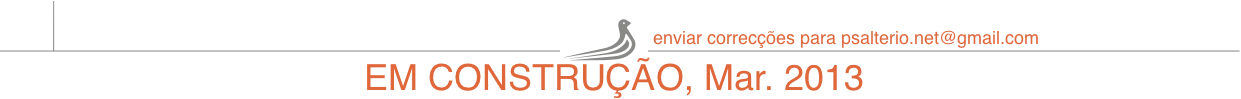
\includegraphics{_images/bkground_page_bottom.png}
}}





% this includes all the guitar tabs that may be needed
% must complete all the chords used in psalterio

% Cb chords

% C chords
\def \gtabCb{\gtab{Cb}{X32010:X32010}}
\def \gtabC{\gtab{C}{X32010:032010}}
\def \gtabCm{\gtab{Cm}{3:113321:004320}}

\def \gtabCsharpSusFour{\gtab{C\#sus4}{4:XX3341:XX2341}}

% Db chords

% D chords
\def \gtabD{\gtab{D}{X00232:000132}}
\def \gtabDm{\gtab{Dm}{X00231:000231}}
\def \gtabDfour{\gtab{D4}{X00233:000134}}
\def \gtabDseven{\gtab{D7}{X00212:000213}}
\def \gtabDsevenPlus{\gtab{D7+}{X00222:000111}}

% D#/Eb chords
\def \gtabDsharp{\gtab{D\#}{2:XX0232:000132}}

% E chords
\def \gtabE{\gtab{E}{022100:023100}}
\def \gtabEseven{\gtab{E}{020100:020100}}

\def \gtabEm{\gtab{Em}{022000:012000}}
\def \gtabEmSeven{\gtab{Em7}{022030:012040}}

% Gb chords

% F chords
\def \gtabF{\gtab{F}{1:133211:034200}}
\def \gtabFm{\gtab{Fm}{1:133111:034000}}


% F# chords
\def \gtabFsharpMinor{\gtab{F\#m}{2:133111:034000}}
\def \gtabFsharpMinorSeven{\gtab{F\#m7}{2:131131:030040}}

% Gb chords

% G chords
\def \gtabG{\gtab{G}{320033:210034}}
\def \gtabGseven{\gtab{G7}{320001:320001}}
\def \gtabGfret{\gtab{(G)}{3:133211:034200}}
\def \gtabGm{\gtab{Gm}{3:133111:034000}}


% G# / Ab chords

% A chords
\def \gtabA{\gtab{A}{X02220:001230}}
\def \gtabAm{\gtab{Am}{X02210:002310}}
\def \gtabAmSeven{\gtab{Am7}{X02010:002010}}
\def \gtabAfour{\gtab{A4}{X02230:001230}}
\def \gtabAseven{\gtab{A7}{X02020:001030}}

% Bb chords
\def \gtabBb{\gtab{Bb}{X13331}}

% B chords
\def \gtabB{\gtab{B}{X13331:003210}}
\def \gtabBm{\gtab{Bm}{X13321:003420}}
\def \gtabBmSeven{\gtab{Bm7}{X13121:003020}}



% after any { or } at the end of a line inside the macro definition add %, otherwise you'll get an extra space
\newcommand{\guitarTab}[1]{%
\ifstrequal{#1}{Cb}      {\gtab{Cb}{X32010:X32010}      }{}%
\ifstrequal{#1}{C}        { \gtab{C}{X32010:032010}       }{}%
%
%G
%
\ifstrequal{#1}{G}       { \gtab{G}{320033:210034}       }{}%
\ifstrequal{#1}{G7}     { \gtab{G7}{320001:320001}     }{}%
\ifstrequal{#1}{Gfret}  { \gtab{G}{3:133211:034200}    }{}%
\ifstrequal{#1}{Gm}    { \gtab{Gm}{3:133111:034000}  }{}%
} %end \newcommand{\gtab}

%muda aqui o numero da musica em que estas a trabalhar
%\def \selectSong{114}

\providebool{gchords}
\setbool{gchords}{true}

% set guitar chords vertical space separation with lyrics
\def \gchordsVspace{5 mm}

\begin{document}
	
	
	\AddToShipoutPicture*{\BottomPic}
	
	\begin{songs}{}
	
	%format file
	%
%Font Sizes
%
%\tiny
%\scriptsize
%\footnotesize
%\small
%\normalsize
%\large
%\Large
%\LARGE
%\huge
%\Huge


%\renewcommand{\thesongnum}{A\arabic{songnum}}
\renewcommand{\printsongnum}[1]{\sffamily\bfseries\huge\MakeUppercase#1}
\setlength{\songnumwidth}{2cm} % box width
%\renewcommand{\snumbgcolor}{white}

%change font for Title
\renewcommand{\stitlefont}{\sffamily\bfseries\huge\MakeUppercase} %song title

%remove verse numbers
%\noversenumbers 
% make left separation
\setlength{\versenumwidth}{2.0cm}

%verse separations
%\versesep=15pt
%\afterpreludeskip=2pt
%\beforepostludeskip=2pt
%\baselineadj=10pt

% separation between chords and lyrics
\renewcommand{\clineparams}{ 
\baselineskip=10pt 
%\lineskiplimit=2pt 
%\lineskip=5pt
}

% change font for lyrics
%\renewcommand{\lyricfont}{\sffamily}
%\renewcommand{\lyricfont}{\sffamily\small}
\renewcommand{\lyricfont}{\sffamily\large}
%\renewcommand{\chorusfont}{\sffamily}
\renewcommand{\chorusfont}{\sffamily\large}

%change the Chords formatting
\renewcommand{\printchord}[1]{\sffamily\color{red}\it\normalsize#1}

%check http://www.tug.org/pracjourn/2006-1/schmidt/schmidt.pdf


%\renewcommand{\songauthors}[1]{tete #1}


%\renewcommand{\extendpostlude}
%{ \songcopyright\ \songlicense\unskip \ Used with permission.}

\setlength{\cbarwidth}{0pt}
\setlength{\sbarheight}{0pt}

% music anf lyrics by
\newcommand{\musicLyricsBy}{} 
\newsongkey{mlby}{\def\musicLyricsBy{}}
                 {\def\musicLyricsBy{\sffamily\it\small letra e música por #1\par}}

% music anf lyrics by
\newcommand{\musicby}{} 
\newsongkey{music}{\def\musicby{}}
                 {\def\musicby{\sffamily\it\small música: #1\par}}

% music anf lyrics by
\newcommand{\lyricsby}{} 
\newsongkey{lyrics}{\def\lyricsby{}}
                 {\def\lyricsby{\sffamily\it\small letra: #1\par}}

%\renewcommand{\sharpsymbol}{\ensuremath{^\sharp}}
\renewcommand{\extendprelude}{
  \showrefs\showauthors 
  %{\bfseries\musicLyricsBy}
  {\bfseries\musicby}
  {\bfseries\lyricsby}
}

\def \gtabsOn{1}
	

%%%%%%%%%%%%%%%%%%%%%%%%%%%%%%%%%%%%%%%%%%%%%%%%%%%%%%%%%%%%%%%%%%%%%%%%%%%
% set song number
%%%%%%%%%%%%%%%%%%%%%%%%%%%%%%%%%%%%%%%%%%%%%%%%%%%%%%%%%%%%%%%%%%%%%%%%%%%
\setcounter{songnum}{23}

%%%%%%%%%%%%%%%%%%%%%%%%%%%%%%%%%%%%%%%%%%%%%%%%%%%%%%%%%%%%%%%%%%%%%%%%%%%
% begin song latex formating, set the title and other info
%%%%%%%%%%%%%%%%%%%%%%%%%%%%%%%%%%%%%%%%%%%%%%%%%%%%%%%%%%%%%%%%%%%%%%%%%%%
% song title
\beginsong{Não Desistir}[
 % music and lyric by
% mlby={},
% lyrics
%lyrics={Autor da Letra}, 
% music by
%music={Autor da Música},
% bible verse
%sr={},
% licence/copyright
%cr={Public domain.},
% arrangement by
%arr={},
% index title
index={Não Desistir}]

%%%%%%%%%%%%%%%%%%%%%%%%%%%%%%%%%%%%%%%%%%%%%%%%%%%%%%%%%%%%%%%%%%%%%%%%%%%
% section #1: verse 
%%%%%%%%%%%%%%%%%%%%%%%%%%%%%%%%%%%%%%%%%%%%%%%%%%%%%%%%%%%%%%%%%%%%%%%%%%%
\beginverse
Dias \[C]há, bem \[G7]sei, em que \[C]triste te \[F]sentes,
Sem \[C]paz, segu\[Am7]rança e \[Ab7G7]fé.
Mas e\[C]xiste al\[G7]guém, que \[C]co\[C7]ragem e \[F]força
Te \[C/G]pode tra\[F/G]zer \[Em]do \[G7 F C]além
\endverse

%%%%%%%%%%%%%%%%%%%%%%%%%%%%%%%%%%%%%%%%%%%%%%%%%%%%%%%%%%%%%%%%%%%%%%%%%%%
% section #2: chorus 
%%%%%%%%%%%%%%%%%%%%%%%%%%%%%%%%%%%%%%%%%%%%%%%%%%%%%%%%%%%%%%%%%%%%%%%%%%%
\beginchorus
Não desis\[C]tir, \[F]Cristo vem \[C G7]logo. \[C]
\[Am/C]Breve \[E/B Am]aurora \[D7]há-\[D11]de ra\[D7]iar.\[F/G G]
Não desis\[C]tir, \[F]Cristo vem \[C G7 F]logo.
Não desis\[C]tir, \[F/G]Ele  \[Em G7 F C Dm7 C]virá
\endchorus

\chordsoff
%%%%%%%%%%%%%%%%%%%%%%%%%%%%%%%%%%%%%%%%%%%%%%%%%%%%%%%%%%%%%%%%%%%%%%%%%%%
% section #3: verse 
%%%%%%%%%%%%%%%%%%%%%%%%%%%%%%%%%%%%%%%%%%%%%%%%%%%%%%%%%%%%%%%%%%%%%%%%%%%
\beginverse
Este mundo, eu sei, não vai muito longe,
E o mal então terá fim.
Minha fé em Deus está bem firmada.
Jesus prometeu, vem óh! sim.
\endverse


%%%%%%%%%%%%%%%%%%%%%%%%%%%%%%%%%%%%%%%%%%%%%%%%%%%%%%%%%%%%%%%%%%%%%%%%%%%
% print guitar tabs used in this song
%%%%%%%%%%%%%%%%%%%%%%%%%%%%%%%%%%%%%%%%%%%%%%%%%%%%%%%%%%%%%%%%%%%%%%%%%%%
% if the guitar chords are to be printed
\ifbool{gchords}{
% set a vertical space of 10 pt 
\vspace{\gchordsVspace}
} % end if

%%%%%%%%%%%%%%%%%%%%%%%%%%%%%%%%%%%%%%%%%%%%%%%%%%%%%%%%%%%%%%%%%%%%%%%%%%%
% end song latex formating
%%%%%%%%%%%%%%%%%%%%%%%%%%%%%%%%%%%%%%%%%%%%%%%%%%%%%%%%%%%%%%%%%%%%%%%%%%%
% end song
\endsong

%include song latex footer
%	 %lilypond-book --output=out --pdf  106single.tex
	 %\lilypondfile[]{E_101.ly}
	
\end{document}	
	%%%%%%%%%%%%%%%%%%%%%%%%%%%%%%%%%%%%%%%%%%%%%%%%%%%%%%%%%%%%%%%%%%%%%%%%%%%
% this has all the necessary packages and formatting for the document
%%%%%%%%%%%%%%%%%%%%%%%%%%%%%%%%%%%%%%%%%%%%%%%%%%%%%%%%%%%%%%%%%%%%%%%%%%%
%\def \includeFolder{../_include}

% this has all the necessary packages and formatting for the document
\documentclass[10pt,a5paper]{article}

%define include folder
\def \includeFolder{_include}

%packages
\usepackage[left=1cm,right=1cm,top=1cm,bottom=1cm]{geometry}

\usepackage[chorded]{\includeFolder/psalterio} %must check the licence to change the name of the sty file!!!
%\usepackage[chorded]{resources/songs-old} %must check the licence to change the name of the sty file!!!

\usepackage[utf8]{inputenc}

\usepackage{graphicx}
\usepackage{wrapfig}
\usepackage{wallpaper}
\usepackage{color}
\usepackage{eso-pic} %for background pictures
\usepackage[bookmarks]{hyperref} 
%\usepackage{ifthen} %etoolbox is more up to date
\usepackage{etoolbox}


%\usepackage[xetex]{graphicx}
%\usepackage{fontspec,xunicode}
%\defaultfontfeatures{Mapping=tex-text,Scale=MatchLowercase}
%\setmainfont[Scale=.95]{Times}
%\setmonofont{Lucida Sans Typewriter}

%\usepackage[portuguese]{babel}
%\usepackage[latin1]{inputenc}
%\usepackage[utf8]{inputenc}
%\usepackage[T1]{fontenc}
%\usepackage[scaled]{uarial}
%\usepackage{helvet}
%\renewcommand{\familydefault}{\sfdefault}

%this removes the page number
\thispagestyle{empty}
\pagestyle{empty}
\songcolumns{1}

\parindent 0pt

%add background picture
\newcommand\BackgroundPic{
\put(0,0){
\parbox[b][\paperheight]{\paperwidth}{%
\vfill
\centering

\includegraphics[width=\paperwidth,height=\paperheight,
keepaspectratio]{logo.png}%
\vfill
}}}

\newcommand\BottomPic{
\put(0,0){
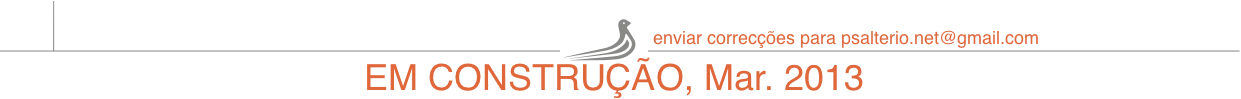
\includegraphics{_images/bkground_page_bottom.png}
}}





% this includes all the guitar tabs that may be needed
% must complete all the chords used in psalterio

% Cb chords

% C chords
\def \gtabCb{\gtab{Cb}{X32010:X32010}}
\def \gtabC{\gtab{C}{X32010:032010}}
\def \gtabCm{\gtab{Cm}{3:113321:004320}}

\def \gtabCsharpSusFour{\gtab{C\#sus4}{4:XX3341:XX2341}}

% Db chords

% D chords
\def \gtabD{\gtab{D}{X00232:000132}}
\def \gtabDm{\gtab{Dm}{X00231:000231}}
\def \gtabDfour{\gtab{D4}{X00233:000134}}
\def \gtabDseven{\gtab{D7}{X00212:000213}}
\def \gtabDsevenPlus{\gtab{D7+}{X00222:000111}}

% D#/Eb chords
\def \gtabDsharp{\gtab{D\#}{2:XX0232:000132}}

% E chords
\def \gtabE{\gtab{E}{022100:023100}}
\def \gtabEseven{\gtab{E}{020100:020100}}

\def \gtabEm{\gtab{Em}{022000:012000}}
\def \gtabEmSeven{\gtab{Em7}{022030:012040}}

% Gb chords

% F chords
\def \gtabF{\gtab{F}{1:133211:034200}}
\def \gtabFm{\gtab{Fm}{1:133111:034000}}


% F# chords
\def \gtabFsharpMinor{\gtab{F\#m}{2:133111:034000}}
\def \gtabFsharpMinorSeven{\gtab{F\#m7}{2:131131:030040}}

% Gb chords

% G chords
\def \gtabG{\gtab{G}{320033:210034}}
\def \gtabGseven{\gtab{G7}{320001:320001}}
\def \gtabGfret{\gtab{(G)}{3:133211:034200}}
\def \gtabGm{\gtab{Gm}{3:133111:034000}}


% G# / Ab chords

% A chords
\def \gtabA{\gtab{A}{X02220:001230}}
\def \gtabAm{\gtab{Am}{X02210:002310}}
\def \gtabAmSeven{\gtab{Am7}{X02010:002010}}
\def \gtabAfour{\gtab{A4}{X02230:001230}}
\def \gtabAseven{\gtab{A7}{X02020:001030}}

% Bb chords
\def \gtabBb{\gtab{Bb}{X13331}}

% B chords
\def \gtabB{\gtab{B}{X13331:003210}}
\def \gtabBm{\gtab{Bm}{X13321:003420}}
\def \gtabBmSeven{\gtab{Bm7}{X13121:003020}}



% after any { or } at the end of a line inside the macro definition add %, otherwise you'll get an extra space
\newcommand{\guitarTab}[1]{%
\ifstrequal{#1}{Cb}      {\gtab{Cb}{X32010:X32010}      }{}%
\ifstrequal{#1}{C}        { \gtab{C}{X32010:032010}       }{}%
%
%G
%
\ifstrequal{#1}{G}       { \gtab{G}{320033:210034}       }{}%
\ifstrequal{#1}{G7}     { \gtab{G7}{320001:320001}     }{}%
\ifstrequal{#1}{Gfret}  { \gtab{G}{3:133211:034200}    }{}%
\ifstrequal{#1}{Gm}    { \gtab{Gm}{3:133111:034000}  }{}%
} %end \newcommand{\gtab}

%muda aqui o numero da musica em que estas a trabalhar
%\def \selectSong{114}

\providebool{gchords}
\setbool{gchords}{true}

% set guitar chords vertical space separation with lyrics
\def \gchordsVspace{5 mm}

\begin{document}
	
	
	\AddToShipoutPicture*{\BottomPic}
	
	\begin{songs}{}
	
	%format file
	%
%Font Sizes
%
%\tiny
%\scriptsize
%\footnotesize
%\small
%\normalsize
%\large
%\Large
%\LARGE
%\huge
%\Huge


%\renewcommand{\thesongnum}{A\arabic{songnum}}
\renewcommand{\printsongnum}[1]{\sffamily\bfseries\huge\MakeUppercase#1}
\setlength{\songnumwidth}{2cm} % box width
%\renewcommand{\snumbgcolor}{white}

%change font for Title
\renewcommand{\stitlefont}{\sffamily\bfseries\huge\MakeUppercase} %song title

%remove verse numbers
%\noversenumbers 
% make left separation
\setlength{\versenumwidth}{2.0cm}

%verse separations
%\versesep=15pt
%\afterpreludeskip=2pt
%\beforepostludeskip=2pt
%\baselineadj=10pt

% separation between chords and lyrics
\renewcommand{\clineparams}{ 
\baselineskip=10pt 
%\lineskiplimit=2pt 
%\lineskip=5pt
}

% change font for lyrics
%\renewcommand{\lyricfont}{\sffamily}
%\renewcommand{\lyricfont}{\sffamily\small}
\renewcommand{\lyricfont}{\sffamily\large}
%\renewcommand{\chorusfont}{\sffamily}
\renewcommand{\chorusfont}{\sffamily\large}

%change the Chords formatting
\renewcommand{\printchord}[1]{\sffamily\color{red}\it\normalsize#1}

%check http://www.tug.org/pracjourn/2006-1/schmidt/schmidt.pdf


%\renewcommand{\songauthors}[1]{tete #1}


%\renewcommand{\extendpostlude}
%{ \songcopyright\ \songlicense\unskip \ Used with permission.}

\setlength{\cbarwidth}{0pt}
\setlength{\sbarheight}{0pt}

% music anf lyrics by
\newcommand{\musicLyricsBy}{} 
\newsongkey{mlby}{\def\musicLyricsBy{}}
                 {\def\musicLyricsBy{\sffamily\it\small letra e música por #1\par}}

% music anf lyrics by
\newcommand{\musicby}{} 
\newsongkey{music}{\def\musicby{}}
                 {\def\musicby{\sffamily\it\small música: #1\par}}

% music anf lyrics by
\newcommand{\lyricsby}{} 
\newsongkey{lyrics}{\def\lyricsby{}}
                 {\def\lyricsby{\sffamily\it\small letra: #1\par}}

%\renewcommand{\sharpsymbol}{\ensuremath{^\sharp}}
\renewcommand{\extendprelude}{
  \showrefs\showauthors 
  %{\bfseries\musicLyricsBy}
  {\bfseries\musicby}
  {\bfseries\lyricsby}
}

\def \gtabsOn{1}
	

%%%%%%%%%%%%%%%%%%%%%%%%%%%%%%%%%%%%%%%%%%%%%%%%%%%%%%%%%%%%%%%%%%%%%%%%%%%
% set song number
%%%%%%%%%%%%%%%%%%%%%%%%%%%%%%%%%%%%%%%%%%%%%%%%%%%%%%%%%%%%%%%%%%%%%%%%%%%
\setcounter{songnum}{24}

%%%%%%%%%%%%%%%%%%%%%%%%%%%%%%%%%%%%%%%%%%%%%%%%%%%%%%%%%%%%%%%%%%%%%%%%%%%
% begin song latex formating, set the title and other info
%%%%%%%%%%%%%%%%%%%%%%%%%%%%%%%%%%%%%%%%%%%%%%%%%%%%%%%%%%%%%%%%%%%%%%%%%%%
% song title
\beginsong{Hoje Sou Feliz}[
        % music and lyric by
        % mlby={},
        % lyrics
        %lyrics={Autor da Letra}, 
        % music by
        %music={Autor da Música},
        % bible verse
        %sr={},
        % licence/copyright
        %cr={Public domain.},
        % arrangement by
        %arr={},
        % index title
        index={Hoje Sou Feliz}]

%%%%%%%%%%%%%%%%%%%%%%%%%%%%%%%%%%%%%%%%%%%%%%%%%%%%%%%%%%%%%%%%%%%%%%%%%%%
% section #1: verse 
%%%%%%%%%%%%%%%%%%%%%%%%%%%%%%%%%%%%%%%%%%%%%%%%%%%%%%%%%%%%%%%%%%%%%%%%%%%
\beginverse
Per\[G]dido \[D7]foi que Ele \[G]me encon\[D7]trou \[G]neste \[G7dim]mundo  \[D7]vil,
To\[D7]mou-me, no seu sangue \[G]me \[D7]la\[Em]vou, \[A7]hoje sou \[D7]feliz!
\endverse

%%%%%%%%%%%%%%%%%%%%%%%%%%%%%%%%%%%%%%%%%%%%%%%%%%%%%%%%%%%%%%%%%%%%%%%%%%%
% section #2: verse 
%%%%%%%%%%%%%%%%%%%%%%%%%%%%%%%%%%%%%%%%%%%%%%%%%%%%%%%%%%%%%%%%%%%%%%%%%%%
\beginverse
Hoje \[G]sou feliz, foi-se meu \[D7]temor,
Vou permanecer \[G]junto \[D7]ao \[G]Sal\[D7]va\[G]dor.
Foi-se a escuridão, \[Em]raia a \[E]luz do \[Am]Céu.
\[C]Pois eu sei que \[G7]sou do meu Senhor,
E \[A7]Ele \[D7]é \[G]meu.
\endverse

\chordsoff
%%%%%%%%%%%%%%%%%%%%%%%%%%%%%%%%%%%%%%%%%%%%%%%%%%%%%%%%%%%%%%%%%%%%%%%%%%%
% section #3: verse 
%%%%%%%%%%%%%%%%%%%%%%%%%%%%%%%%%%%%%%%%%%%%%%%%%%%%%%%%%%%%%%%%%%%%%%%%%%%
\beginverse
Se muitas tentações me sobrevêm, para Ele vou,
Recebo forças que a mim convêm, se com Ele estou!
\endverse

%%%%%%%%%%%%%%%%%%%%%%%%%%%%%%%%%%%%%%%%%%%%%%%%%%%%%%%%%%%%%%%%%%%%%%%%%%%
% section #4: verse 
%%%%%%%%%%%%%%%%%%%%%%%%%%%%%%%%%%%%%%%%%%%%%%%%%%%%%%%%%%%%%%%%%%%%%%%%%%%
\beginverse
Se negra noite assustar-me vem, ouço a Sua voz,
As trevas tornam-se na luz do Sol, com o meu Salvador!
\endverse


%%%%%%%%%%%%%%%%%%%%%%%%%%%%%%%%%%%%%%%%%%%%%%%%%%%%%%%%%%%%%%%%%%%%%%%%%%%
% print guitar tabs used in this song
%%%%%%%%%%%%%%%%%%%%%%%%%%%%%%%%%%%%%%%%%%%%%%%%%%%%%%%%%%%%%%%%%%%%%%%%%%%
% if the guitar chords are to be printed
\ifbool{gchords}{
% set a vertical space of 10 pt 
\vspace{\gchordsVspace}
} % end if

%%%%%%%%%%%%%%%%%%%%%%%%%%%%%%%%%%%%%%%%%%%%%%%%%%%%%%%%%%%%%%%%%%%%%%%%%%%
% end song latex formating
%%%%%%%%%%%%%%%%%%%%%%%%%%%%%%%%%%%%%%%%%%%%%%%%%%%%%%%%%%%%%%%%%%%%%%%%%%%
% end song
\endsong

%include song latex footer
%	 %lilypond-book --output=out --pdf  106single.tex
	 %\lilypondfile[]{E_101.ly}
	
\end{document}
	%%%%%%%%%%%%%%%%%%%%%%%%%%%%%%%%%%%%%%%%%%%%%%%%%%%%%%%%%%%%%%%%%%%%%%%%%%%
% this has all the necessary packages and formatting for the document
%%%%%%%%%%%%%%%%%%%%%%%%%%%%%%%%%%%%%%%%%%%%%%%%%%%%%%%%%%%%%%%%%%%%%%%%%%%
%\def \includeFolder{../_include}

% this has all the necessary packages and formatting for the document
\documentclass[10pt,a5paper]{article}

%define include folder
\def \includeFolder{_include}

%packages
\usepackage[left=1cm,right=1cm,top=1cm,bottom=1cm]{geometry}

\usepackage[chorded]{\includeFolder/psalterio} %must check the licence to change the name of the sty file!!!
%\usepackage[chorded]{resources/songs-old} %must check the licence to change the name of the sty file!!!

\usepackage[utf8]{inputenc}

\usepackage{graphicx}
\usepackage{wrapfig}
\usepackage{wallpaper}
\usepackage{color}
\usepackage{eso-pic} %for background pictures
\usepackage[bookmarks]{hyperref} 
%\usepackage{ifthen} %etoolbox is more up to date
\usepackage{etoolbox}


%\usepackage[xetex]{graphicx}
%\usepackage{fontspec,xunicode}
%\defaultfontfeatures{Mapping=tex-text,Scale=MatchLowercase}
%\setmainfont[Scale=.95]{Times}
%\setmonofont{Lucida Sans Typewriter}

%\usepackage[portuguese]{babel}
%\usepackage[latin1]{inputenc}
%\usepackage[utf8]{inputenc}
%\usepackage[T1]{fontenc}
%\usepackage[scaled]{uarial}
%\usepackage{helvet}
%\renewcommand{\familydefault}{\sfdefault}

%this removes the page number
\thispagestyle{empty}
\pagestyle{empty}
\songcolumns{1}

\parindent 0pt

%add background picture
\newcommand\BackgroundPic{
\put(0,0){
\parbox[b][\paperheight]{\paperwidth}{%
\vfill
\centering

\includegraphics[width=\paperwidth,height=\paperheight,
keepaspectratio]{logo.png}%
\vfill
}}}

\newcommand\BottomPic{
\put(0,0){
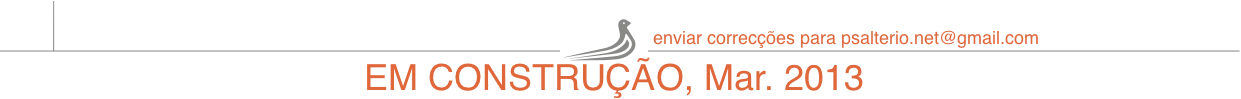
\includegraphics{_images/bkground_page_bottom.png}
}}





% this includes all the guitar tabs that may be needed
% must complete all the chords used in psalterio

% Cb chords

% C chords
\def \gtabCb{\gtab{Cb}{X32010:X32010}}
\def \gtabC{\gtab{C}{X32010:032010}}
\def \gtabCm{\gtab{Cm}{3:113321:004320}}

\def \gtabCsharpSusFour{\gtab{C\#sus4}{4:XX3341:XX2341}}

% Db chords

% D chords
\def \gtabD{\gtab{D}{X00232:000132}}
\def \gtabDm{\gtab{Dm}{X00231:000231}}
\def \gtabDfour{\gtab{D4}{X00233:000134}}
\def \gtabDseven{\gtab{D7}{X00212:000213}}
\def \gtabDsevenPlus{\gtab{D7+}{X00222:000111}}

% D#/Eb chords
\def \gtabDsharp{\gtab{D\#}{2:XX0232:000132}}

% E chords
\def \gtabE{\gtab{E}{022100:023100}}
\def \gtabEseven{\gtab{E}{020100:020100}}

\def \gtabEm{\gtab{Em}{022000:012000}}
\def \gtabEmSeven{\gtab{Em7}{022030:012040}}

% Gb chords

% F chords
\def \gtabF{\gtab{F}{1:133211:034200}}
\def \gtabFm{\gtab{Fm}{1:133111:034000}}


% F# chords
\def \gtabFsharpMinor{\gtab{F\#m}{2:133111:034000}}
\def \gtabFsharpMinorSeven{\gtab{F\#m7}{2:131131:030040}}

% Gb chords

% G chords
\def \gtabG{\gtab{G}{320033:210034}}
\def \gtabGseven{\gtab{G7}{320001:320001}}
\def \gtabGfret{\gtab{(G)}{3:133211:034200}}
\def \gtabGm{\gtab{Gm}{3:133111:034000}}


% G# / Ab chords

% A chords
\def \gtabA{\gtab{A}{X02220:001230}}
\def \gtabAm{\gtab{Am}{X02210:002310}}
\def \gtabAmSeven{\gtab{Am7}{X02010:002010}}
\def \gtabAfour{\gtab{A4}{X02230:001230}}
\def \gtabAseven{\gtab{A7}{X02020:001030}}

% Bb chords
\def \gtabBb{\gtab{Bb}{X13331}}

% B chords
\def \gtabB{\gtab{B}{X13331:003210}}
\def \gtabBm{\gtab{Bm}{X13321:003420}}
\def \gtabBmSeven{\gtab{Bm7}{X13121:003020}}



% after any { or } at the end of a line inside the macro definition add %, otherwise you'll get an extra space
\newcommand{\guitarTab}[1]{%
\ifstrequal{#1}{Cb}      {\gtab{Cb}{X32010:X32010}      }{}%
\ifstrequal{#1}{C}        { \gtab{C}{X32010:032010}       }{}%
%
%G
%
\ifstrequal{#1}{G}       { \gtab{G}{320033:210034}       }{}%
\ifstrequal{#1}{G7}     { \gtab{G7}{320001:320001}     }{}%
\ifstrequal{#1}{Gfret}  { \gtab{G}{3:133211:034200}    }{}%
\ifstrequal{#1}{Gm}    { \gtab{Gm}{3:133111:034000}  }{}%
} %end \newcommand{\gtab}

%muda aqui o numero da musica em que estas a trabalhar
%\def \selectSong{114}

\providebool{gchords}
\setbool{gchords}{true}

% set guitar chords vertical space separation with lyrics
\def \gchordsVspace{5 mm}

\begin{document}
	
	
	\AddToShipoutPicture*{\BottomPic}
	
	\begin{songs}{}
	
	%format file
	%
%Font Sizes
%
%\tiny
%\scriptsize
%\footnotesize
%\small
%\normalsize
%\large
%\Large
%\LARGE
%\huge
%\Huge


%\renewcommand{\thesongnum}{A\arabic{songnum}}
\renewcommand{\printsongnum}[1]{\sffamily\bfseries\huge\MakeUppercase#1}
\setlength{\songnumwidth}{2cm} % box width
%\renewcommand{\snumbgcolor}{white}

%change font for Title
\renewcommand{\stitlefont}{\sffamily\bfseries\huge\MakeUppercase} %song title

%remove verse numbers
%\noversenumbers 
% make left separation
\setlength{\versenumwidth}{2.0cm}

%verse separations
%\versesep=15pt
%\afterpreludeskip=2pt
%\beforepostludeskip=2pt
%\baselineadj=10pt

% separation between chords and lyrics
\renewcommand{\clineparams}{ 
\baselineskip=10pt 
%\lineskiplimit=2pt 
%\lineskip=5pt
}

% change font for lyrics
%\renewcommand{\lyricfont}{\sffamily}
%\renewcommand{\lyricfont}{\sffamily\small}
\renewcommand{\lyricfont}{\sffamily\large}
%\renewcommand{\chorusfont}{\sffamily}
\renewcommand{\chorusfont}{\sffamily\large}

%change the Chords formatting
\renewcommand{\printchord}[1]{\sffamily\color{red}\it\normalsize#1}

%check http://www.tug.org/pracjourn/2006-1/schmidt/schmidt.pdf


%\renewcommand{\songauthors}[1]{tete #1}


%\renewcommand{\extendpostlude}
%{ \songcopyright\ \songlicense\unskip \ Used with permission.}

\setlength{\cbarwidth}{0pt}
\setlength{\sbarheight}{0pt}

% music anf lyrics by
\newcommand{\musicLyricsBy}{} 
\newsongkey{mlby}{\def\musicLyricsBy{}}
                 {\def\musicLyricsBy{\sffamily\it\small letra e música por #1\par}}

% music anf lyrics by
\newcommand{\musicby}{} 
\newsongkey{music}{\def\musicby{}}
                 {\def\musicby{\sffamily\it\small música: #1\par}}

% music anf lyrics by
\newcommand{\lyricsby}{} 
\newsongkey{lyrics}{\def\lyricsby{}}
                 {\def\lyricsby{\sffamily\it\small letra: #1\par}}

%\renewcommand{\sharpsymbol}{\ensuremath{^\sharp}}
\renewcommand{\extendprelude}{
  \showrefs\showauthors 
  %{\bfseries\musicLyricsBy}
  {\bfseries\musicby}
  {\bfseries\lyricsby}
}

\def \gtabsOn{1}
	

%%%%%%%%%%%%%%%%%%%%%%%%%%%%%%%%%%%%%%%%%%%%%%%%%%%%%%%%%%%%%%%%%%%%%%%%%%%
% set song number
%%%%%%%%%%%%%%%%%%%%%%%%%%%%%%%%%%%%%%%%%%%%%%%%%%%%%%%%%%%%%%%%%%%%%%%%%%%
\setcounter{songnum}{25}

%%%%%%%%%%%%%%%%%%%%%%%%%%%%%%%%%%%%%%%%%%%%%%%%%%%%%%%%%%%%%%%%%%%%%%%%%%%
% begin song latex formating, set the title and other info
%%%%%%%%%%%%%%%%%%%%%%%%%%%%%%%%%%%%%%%%%%%%%%%%%%%%%%%%%%%%%%%%%%%%%%%%%%%
% song title
\beginsong{L’amour du Sauveur}[
% music and lyric by
% mlby={},
% lyrics
%lyrics={}, 
% music by
%music={},
% bible verse
%sr={},
% licence/copyright
%cr={Public domain.},
% arrangement by
%arr={},
% index title
index={L’amour du Sauveur}]

%%%%%%%%%%%%%%%%%%%%%%%%%%%%%%%%%%%%%%%%%%%%%%%%%%%%%%%%%%%%%%%%%%%%%%%%%%%
% section #1: verse 
%%%%%%%%%%%%%%%%%%%%%%%%%%%%%%%%%%%%%%%%%%%%%%%%%%%%%%%%%%%%%%%%%%%%%%%%%%%
\beginverse
L’a\[Db]mour du Sauveur, tel un vaste océan,
\[Db7Gb]Inonde mon c\[Db]oeur \[Db7dim]de son flot puiss\[Ab7]ant.
Il \[Db]est doux et t\[Ab]ender, im\[Bbm]mense, infi\[F]ni,
Et p\[Bbm]our \[Gb]toujours \[Db  AbDb]me suffit.
\endverse

%%%%%%%%%%%%%%%%%%%%%%%%%%%%%%%%%%%%%%%%%%%%%%%%%%%%%%%%%%%%%%%%%%%%%%%%%%%
% section #2: verse 
%%%%%%%%%%%%%%%%%%%%%%%%%%%%%%%%%%%%%%%%%%%%%%%%%%%%%%%%%%%%%%%%%%%%%%%%%%%
\beginverse

\endverse


%%%%%%%%%%%%%%%%%%%%%%%%%%%%%%%%%%%%%%%%%%%%%%%%%%%%%%%%%%%%%%%%%%%%%%%%%%%
% print guitar tabs used in this song
%%%%%%%%%%%%%%%%%%%%%%%%%%%%%%%%%%%%%%%%%%%%%%%%%%%%%%%%%%%%%%%%%%%%%%%%%%%
% if the guitar chords are to be printed
\ifbool{gchords}{
% set a vertical space of 10 pt 
\vspace{\gchordsVspace}
} % end if

%%%%%%%%%%%%%%%%%%%%%%%%%%%%%%%%%%%%%%%%%%%%%%%%%%%%%%%%%%%%%%%%%%%%%%%%%%%
% end song latex formating
%%%%%%%%%%%%%%%%%%%%%%%%%%%%%%%%%%%%%%%%%%%%%%%%%%%%%%%%%%%%%%%%%%%%%%%%%%%
% end song
\endsong

%include song latex footer
%	 %lilypond-book --output=out --pdf  106single.tex
	 %\lilypondfile[]{E_101.ly}
	
\end{document}
	%%%%%%%%%%%%%%%%%%%%%%%%%%%%%%%%%%%%%%%%%%%%%%%%%%%%%%%%%%%%%%%%%%%%%%%%%%%
% this has all the necessary packages and formatting for the document
%%%%%%%%%%%%%%%%%%%%%%%%%%%%%%%%%%%%%%%%%%%%%%%%%%%%%%%%%%%%%%%%%%%%%%%%%%%
%\def \includeFolder{../_include}

% this has all the necessary packages and formatting for the document
\documentclass[10pt,a5paper]{article}

%define include folder
\def \includeFolder{_include}

%packages
\usepackage[left=1cm,right=1cm,top=1cm,bottom=1cm]{geometry}

\usepackage[chorded]{\includeFolder/psalterio} %must check the licence to change the name of the sty file!!!
%\usepackage[chorded]{resources/songs-old} %must check the licence to change the name of the sty file!!!

\usepackage[utf8]{inputenc}

\usepackage{graphicx}
\usepackage{wrapfig}
\usepackage{wallpaper}
\usepackage{color}
\usepackage{eso-pic} %for background pictures
\usepackage[bookmarks]{hyperref} 
%\usepackage{ifthen} %etoolbox is more up to date
\usepackage{etoolbox}


%\usepackage[xetex]{graphicx}
%\usepackage{fontspec,xunicode}
%\defaultfontfeatures{Mapping=tex-text,Scale=MatchLowercase}
%\setmainfont[Scale=.95]{Times}
%\setmonofont{Lucida Sans Typewriter}

%\usepackage[portuguese]{babel}
%\usepackage[latin1]{inputenc}
%\usepackage[utf8]{inputenc}
%\usepackage[T1]{fontenc}
%\usepackage[scaled]{uarial}
%\usepackage{helvet}
%\renewcommand{\familydefault}{\sfdefault}

%this removes the page number
\thispagestyle{empty}
\pagestyle{empty}
\songcolumns{1}

\parindent 0pt

%add background picture
\newcommand\BackgroundPic{
\put(0,0){
\parbox[b][\paperheight]{\paperwidth}{%
\vfill
\centering
\includegraphics[width=\paperwidth,height=\paperheight,
keepaspectratio]{logo.png}%
\vfill
}}}

\newcommand\BottomPic{
\put(0,0){
\includegraphics{_images/bkground_page_bottom.png}
}}





% this includes all the guitar tabs that may be needed
% must complete all the chords used in psalterio

% Cb chords

% C chords
\def \gtabCb{\gtab{Cb}{X32010:X32010}}
\def \gtabC{\gtab{C}{X32010:032010}}
\def \gtabCm{\gtab{Cm}{3:113321:004320}}

\def \gtabCsharpSusFour{\gtab{C\#sus4}{4:XX3341:XX2341}}

% Db chords

% D chords
\def \gtabD{\gtab{D}{X00232:000132}}
\def \gtabDm{\gtab{Dm}{X00231:000231}}
\def \gtabDfour{\gtab{D4}{X00233:000134}}
\def \gtabDseven{\gtab{D7}{X00212:000213}}
\def \gtabDsevenPlus{\gtab{D7+}{X00222:000111}}

% D#/Eb chords
\def \gtabDsharp{\gtab{D\#}{2:XX0232:000132}}

% E chords
\def \gtabE{\gtab{E}{022100:023100}}
\def \gtabEseven{\gtab{E}{020100:020100}}

\def \gtabEm{\gtab{Em}{022000:012000}}
\def \gtabEmSeven{\gtab{Em7}{022030:012040}}

% Gb chords

% F chords
\def \gtabF{\gtab{F}{1:133211:034200}}
\def \gtabFm{\gtab{Fm}{1:133111:034000}}


% F# chords
\def \gtabFsharpMinor{\gtab{F\#m}{2:133111:034000}}
\def \gtabFsharpMinorSeven{\gtab{F\#m7}{2:131131:030040}}

% Gb chords

% G chords
\def \gtabG{\gtab{G}{320033:210034}}
\def \gtabGseven{\gtab{G7}{320001:320001}}
\def \gtabGfret{\gtab{(G)}{3:133211:034200}}
\def \gtabGm{\gtab{Gm}{3:133111:034000}}


% G# / Ab chords

% A chords
\def \gtabA{\gtab{A}{X02220:001230}}
\def \gtabAm{\gtab{Am}{X02210:002310}}
\def \gtabAmSeven{\gtab{Am7}{X02010:002010}}
\def \gtabAfour{\gtab{A4}{X02230:001230}}
\def \gtabAseven{\gtab{A7}{X02020:001030}}

% Bb chords
\def \gtabBb{\gtab{Bb}{X13331}}

% B chords
\def \gtabB{\gtab{B}{X13331:003210}}
\def \gtabBm{\gtab{Bm}{X13321:003420}}
\def \gtabBmSeven{\gtab{Bm7}{X13121:003020}}



% after any { or } at the end of a line inside the macro definition add %, otherwise you'll get an extra space
\newcommand{\guitarTab}[1]{%
\ifstrequal{#1}{Cb}      {\gtab{Cb}{X32010:X32010}      }{}%
\ifstrequal{#1}{C}        { \gtab{C}{X32010:032010}       }{}%
%
%G
%
\ifstrequal{#1}{G}       { \gtab{G}{320033:210034}       }{}%
\ifstrequal{#1}{G7}     { \gtab{G7}{320001:320001}     }{}%
\ifstrequal{#1}{Gfret}  { \gtab{G}{3:133211:034200}    }{}%
\ifstrequal{#1}{Gm}    { \gtab{Gm}{3:133111:034000}  }{}%
} %end \newcommand{\gtab}

%muda aqui o numero da musica em que estas a trabalhar
%\def \selectSong{114}

\providebool{gchords}
\setbool{gchords}{true}

% set guitar chords vertical space separation with lyrics
\def \gchordsVspace{5 mm}

\begin{document}
	
	
	\AddToShipoutPicture*{\BottomPic}
	
	\begin{songs}{}
	
	%format file
	%
%Font Sizes
%
%\tiny
%\scriptsize
%\footnotesize
%\small
%\normalsize
%\large
%\Large
%\LARGE
%\huge
%\Huge


%\renewcommand{\thesongnum}{A\arabic{songnum}}
\renewcommand{\printsongnum}[1]{\sffamily\bfseries\huge\MakeUppercase#1}
\setlength{\songnumwidth}{2cm} % box width
%\renewcommand{\snumbgcolor}{white}

%change font for Title
\renewcommand{\stitlefont}{\sffamily\bfseries\huge\MakeUppercase} %song title

%remove verse numbers
%\noversenumbers 
% make left separation
\setlength{\versenumwidth}{2.0cm}

%verse separations
%\versesep=15pt
%\afterpreludeskip=2pt
%\beforepostludeskip=2pt
%\baselineadj=10pt

% separation between chords and lyrics
\renewcommand{\clineparams}{ 
\baselineskip=10pt 
%\lineskiplimit=2pt 
%\lineskip=5pt
}

% change font for lyrics
%\renewcommand{\lyricfont}{\sffamily}
%\renewcommand{\lyricfont}{\sffamily\small}
\renewcommand{\lyricfont}{\sffamily\large}
%\renewcommand{\chorusfont}{\sffamily}
\renewcommand{\chorusfont}{\sffamily\large}

%change the Chords formatting
\renewcommand{\printchord}[1]{\sffamily\color{red}\it\normalsize#1}

%check http://www.tug.org/pracjourn/2006-1/schmidt/schmidt.pdf


%\renewcommand{\songauthors}[1]{tete #1}


%\renewcommand{\extendpostlude}
%{ \songcopyright\ \songlicense\unskip \ Used with permission.}

\setlength{\cbarwidth}{0pt}
\setlength{\sbarheight}{0pt}

% music anf lyrics by
\newcommand{\musicLyricsBy}{} 
\newsongkey{mlby}{\def\musicLyricsBy{}}
                 {\def\musicLyricsBy{\sffamily\it\small letra e música por #1\par}}

% music anf lyrics by
\newcommand{\musicby}{} 
\newsongkey{music}{\def\musicby{}}
                 {\def\musicby{\sffamily\it\small música: #1\par}}

% music anf lyrics by
\newcommand{\lyricsby}{} 
\newsongkey{lyrics}{\def\lyricsby{}}
                 {\def\lyricsby{\sffamily\it\small letra: #1\par}}

%\renewcommand{\sharpsymbol}{\ensuremath{^\sharp}}
\renewcommand{\extendprelude}{
  \showrefs\showauthors 
  %{\bfseries\musicLyricsBy}
  {\bfseries\musicby}
  {\bfseries\lyricsby}
}

\def \gtabsOn{1}
	

%%%%%%%%%%%%%%%%%%%%%%%%%%%%%%%%%%%%%%%%%%%%%%%%%%%%%%%%%%%%%%%%%%%%%%%%%%%
% set song number
%%%%%%%%%%%%%%%%%%%%%%%%%%%%%%%%%%%%%%%%%%%%%%%%%%%%%%%%%%%%%%%%%%%%%%%%%%%
\setcounter{songnum}{26}

%%%%%%%%%%%%%%%%%%%%%%%%%%%%%%%%%%%%%%%%%%%%%%%%%%%%%%%%%%%%%%%%%%%%%%%%%%%
% begin song latex formating, set the title and other info
%%%%%%%%%%%%%%%%%%%%%%%%%%%%%%%%%%%%%%%%%%%%%%%%%%%%%%%%%%%%%%%%%%%%%%%%%%%
% song title
\beginsong{Canta a Alegria}[
        % music and lyric by
        % mlby={},
        % lyrics
        %lyrics={}, 
        % music by
        %music={},
        % bible verse
        %sr={},
        % licence/copyright
        %cr={Public domain.},
        % arrangement by
        %arr={},
        % index title
        index={Canta a Alegria}]

%%%%%%%%%%%%%%%%%%%%%%%%%%%%%%%%%%%%%%%%%%%%%%%%%%%%%%%%%%%%%%%%%%%%%%%%%%%
% section #1: verse 
%%%%%%%%%%%%%%%%%%%%%%%%%%%%%%%%%%%%%%%%%%%%%%%%%%%%%%%%%%%%%%%%%%%%%%%%%%%
\beginverse
Vou \[F]cantando, na \[Bb]alegria \[C7]de \[F]viver,
A canção que toda a \[Bb]gente vai \[C7]apren\[F]der,
A can\[Bb]ção de \[C7]paz \[F]que \[C7]não tem \[F]dor,
A can\[Bb]ção de \[C7]paz, \[F]que \[C7]traz o \[F]amor,  
A canção do \[Bb]amor que \[C7]assim \[F]diz:
“Não há nada que te \[Bb]possa tornar \[C7]in\[F]feliz”.
\endverse

\chordsoff
%%%%%%%%%%%%%%%%%%%%%%%%%%%%%%%%%%%%%%%%%%%%%%%%%%%%%%%%%%%%%%%%%%%%%%%%%%%
% section #2: verse 
%%%%%%%%%%%%%%%%%%%%%%%%%%%%%%%%%%%%%%%%%%%%%%%%%%%%%%%%%%%%%%%%%%%%%%%%%%%
\beginverse
De manhã, eu me levanto com o sol.
Nem a chuva diminui meu arrebol!
Pela tarde, eu canto um hino ao meu Senhor,
Pois eu sei que nunca é tarde para o amor.
Pela noite adentro eu vou cantar:
“Minha vida é um eterno caminhar.
\endverse


%%%%%%%%%%%%%%%%%%%%%%%%%%%%%%%%%%%%%%%%%%%%%%%%%%%%%%%%%%%%%%%%%%%%%%%%%%%
% print guitar tabs used in this song
%%%%%%%%%%%%%%%%%%%%%%%%%%%%%%%%%%%%%%%%%%%%%%%%%%%%%%%%%%%%%%%%%%%%%%%%%%%
% if the guitar chords are to be printed
\ifbool{gchords}{
% set a vertical space of 10 pt 
\vspace{\gchordsVspace}
} % end if

%%%%%%%%%%%%%%%%%%%%%%%%%%%%%%%%%%%%%%%%%%%%%%%%%%%%%%%%%%%%%%%%%%%%%%%%%%%
% end song latex formating
%%%%%%%%%%%%%%%%%%%%%%%%%%%%%%%%%%%%%%%%%%%%%%%%%%%%%%%%%%%%%%%%%%%%%%%%%%%
% end song
\endsong

%include song latex footer
%	 %lilypond-book --output=out --pdf  106single.tex
	 %\lilypondfile[]{E_101.ly}
	
\end{document}
	%%%%%%%%%%%%%%%%%%%%%%%%%%%%%%%%%%%%%%%%%%%%%%%%%%%%%%%%%%%%%%%%%%%%%%%%%%%
% this has all the necessary packages and formatting for the document
%%%%%%%%%%%%%%%%%%%%%%%%%%%%%%%%%%%%%%%%%%%%%%%%%%%%%%%%%%%%%%%%%%%%%%%%%%%
%\def \includeFolder{../_include}

% this has all the necessary packages and formatting for the document
\documentclass[10pt,a5paper]{article}

%define include folder
\def \includeFolder{_include}

%packages
\usepackage[left=1cm,right=1cm,top=1cm,bottom=1cm]{geometry}

\usepackage[chorded]{\includeFolder/psalterio} %must check the licence to change the name of the sty file!!!
%\usepackage[chorded]{resources/songs-old} %must check the licence to change the name of the sty file!!!

\usepackage[utf8]{inputenc}

\usepackage{graphicx}
\usepackage{wrapfig}
\usepackage{wallpaper}
\usepackage{color}
\usepackage{eso-pic} %for background pictures
\usepackage[bookmarks]{hyperref} 
%\usepackage{ifthen} %etoolbox is more up to date
\usepackage{etoolbox}


%\usepackage[xetex]{graphicx}
%\usepackage{fontspec,xunicode}
%\defaultfontfeatures{Mapping=tex-text,Scale=MatchLowercase}
%\setmainfont[Scale=.95]{Times}
%\setmonofont{Lucida Sans Typewriter}

%\usepackage[portuguese]{babel}
%\usepackage[latin1]{inputenc}
%\usepackage[utf8]{inputenc}
%\usepackage[T1]{fontenc}
%\usepackage[scaled]{uarial}
%\usepackage{helvet}
%\renewcommand{\familydefault}{\sfdefault}

%this removes the page number
\thispagestyle{empty}
\pagestyle{empty}
\songcolumns{1}

\parindent 0pt

%add background picture
\newcommand\BackgroundPic{
\put(0,0){
\parbox[b][\paperheight]{\paperwidth}{%
\vfill
\centering
\includegraphics[width=\paperwidth,height=\paperheight,
keepaspectratio]{logo.png}%
\vfill
}}}

\newcommand\BottomPic{
\put(0,0){
\includegraphics{_images/bkground_page_bottom.png}
}}





% this includes all the guitar tabs that may be needed
% must complete all the chords used in psalterio

% Cb chords

% C chords
\def \gtabCb{\gtab{Cb}{X32010:X32010}}
\def \gtabC{\gtab{C}{X32010:032010}}
\def \gtabCm{\gtab{Cm}{3:113321:004320}}

\def \gtabCsharpSusFour{\gtab{C\#sus4}{4:XX3341:XX2341}}

% Db chords

% D chords
\def \gtabD{\gtab{D}{X00232:000132}}
\def \gtabDm{\gtab{Dm}{X00231:000231}}
\def \gtabDfour{\gtab{D4}{X00233:000134}}
\def \gtabDseven{\gtab{D7}{X00212:000213}}
\def \gtabDsevenPlus{\gtab{D7+}{X00222:000111}}

% D#/Eb chords
\def \gtabDsharp{\gtab{D\#}{2:XX0232:000132}}

% E chords
\def \gtabE{\gtab{E}{022100:023100}}
\def \gtabEseven{\gtab{E}{020100:020100}}

\def \gtabEm{\gtab{Em}{022000:012000}}
\def \gtabEmSeven{\gtab{Em7}{022030:012040}}

% Gb chords

% F chords
\def \gtabF{\gtab{F}{1:133211:034200}}
\def \gtabFm{\gtab{Fm}{1:133111:034000}}


% F# chords
\def \gtabFsharpMinor{\gtab{F\#m}{2:133111:034000}}
\def \gtabFsharpMinorSeven{\gtab{F\#m7}{2:131131:030040}}

% Gb chords

% G chords
\def \gtabG{\gtab{G}{320033:210034}}
\def \gtabGseven{\gtab{G7}{320001:320001}}
\def \gtabGfret{\gtab{(G)}{3:133211:034200}}
\def \gtabGm{\gtab{Gm}{3:133111:034000}}


% G# / Ab chords

% A chords
\def \gtabA{\gtab{A}{X02220:001230}}
\def \gtabAm{\gtab{Am}{X02210:002310}}
\def \gtabAmSeven{\gtab{Am7}{X02010:002010}}
\def \gtabAfour{\gtab{A4}{X02230:001230}}
\def \gtabAseven{\gtab{A7}{X02020:001030}}

% Bb chords
\def \gtabBb{\gtab{Bb}{X13331}}

% B chords
\def \gtabB{\gtab{B}{X13331:003210}}
\def \gtabBm{\gtab{Bm}{X13321:003420}}
\def \gtabBmSeven{\gtab{Bm7}{X13121:003020}}



% after any { or } at the end of a line inside the macro definition add %, otherwise you'll get an extra space
\newcommand{\guitarTab}[1]{%
\ifstrequal{#1}{Cb}      {\gtab{Cb}{X32010:X32010}      }{}%
\ifstrequal{#1}{C}        { \gtab{C}{X32010:032010}       }{}%
%
%G
%
\ifstrequal{#1}{G}       { \gtab{G}{320033:210034}       }{}%
\ifstrequal{#1}{G7}     { \gtab{G7}{320001:320001}     }{}%
\ifstrequal{#1}{Gfret}  { \gtab{G}{3:133211:034200}    }{}%
\ifstrequal{#1}{Gm}    { \gtab{Gm}{3:133111:034000}  }{}%
} %end \newcommand{\gtab}

%muda aqui o numero da musica em que estas a trabalhar
%\def \selectSong{114}

\providebool{gchords}
\setbool{gchords}{true}

% set guitar chords vertical space separation with lyrics
\def \gchordsVspace{5 mm}

\begin{document}
	
	
	\AddToShipoutPicture*{\BottomPic}
	
	\begin{songs}{}
	
	%format file
	%
%Font Sizes
%
%\tiny
%\scriptsize
%\footnotesize
%\small
%\normalsize
%\large
%\Large
%\LARGE
%\huge
%\Huge


%\renewcommand{\thesongnum}{A\arabic{songnum}}
\renewcommand{\printsongnum}[1]{\sffamily\bfseries\huge\MakeUppercase#1}
\setlength{\songnumwidth}{2cm} % box width
%\renewcommand{\snumbgcolor}{white}

%change font for Title
\renewcommand{\stitlefont}{\sffamily\bfseries\huge\MakeUppercase} %song title

%remove verse numbers
%\noversenumbers 
% make left separation
\setlength{\versenumwidth}{2.0cm}

%verse separations
%\versesep=15pt
%\afterpreludeskip=2pt
%\beforepostludeskip=2pt
%\baselineadj=10pt

% separation between chords and lyrics
\renewcommand{\clineparams}{ 
\baselineskip=10pt 
%\lineskiplimit=2pt 
%\lineskip=5pt
}

% change font for lyrics
%\renewcommand{\lyricfont}{\sffamily}
%\renewcommand{\lyricfont}{\sffamily\small}
\renewcommand{\lyricfont}{\sffamily\large}
%\renewcommand{\chorusfont}{\sffamily}
\renewcommand{\chorusfont}{\sffamily\large}

%change the Chords formatting
\renewcommand{\printchord}[1]{\sffamily\color{red}\it\normalsize#1}

%check http://www.tug.org/pracjourn/2006-1/schmidt/schmidt.pdf


%\renewcommand{\songauthors}[1]{tete #1}


%\renewcommand{\extendpostlude}
%{ \songcopyright\ \songlicense\unskip \ Used with permission.}

\setlength{\cbarwidth}{0pt}
\setlength{\sbarheight}{0pt}

% music anf lyrics by
\newcommand{\musicLyricsBy}{} 
\newsongkey{mlby}{\def\musicLyricsBy{}}
                 {\def\musicLyricsBy{\sffamily\it\small letra e música por #1\par}}

% music anf lyrics by
\newcommand{\musicby}{} 
\newsongkey{music}{\def\musicby{}}
                 {\def\musicby{\sffamily\it\small música: #1\par}}

% music anf lyrics by
\newcommand{\lyricsby}{} 
\newsongkey{lyrics}{\def\lyricsby{}}
                 {\def\lyricsby{\sffamily\it\small letra: #1\par}}

%\renewcommand{\sharpsymbol}{\ensuremath{^\sharp}}
\renewcommand{\extendprelude}{
  \showrefs\showauthors 
  %{\bfseries\musicLyricsBy}
  {\bfseries\musicby}
  {\bfseries\lyricsby}
}

\def \gtabsOn{1}
	

%%%%%%%%%%%%%%%%%%%%%%%%%%%%%%%%%%%%%%%%%%%%%%%%%%%%%%%%%%%%%%%%%%%%%%%%%%%
% set song number
%%%%%%%%%%%%%%%%%%%%%%%%%%%%%%%%%%%%%%%%%%%%%%%%%%%%%%%%%%%%%%%%%%%%%%%%%%%
\setcounter{songnum}{27}

%%%%%%%%%%%%%%%%%%%%%%%%%%%%%%%%%%%%%%%%%%%%%%%%%%%%%%%%%%%%%%%%%%%%%%%%%%%
% begin song latex formating, set the title and other info
%%%%%%%%%%%%%%%%%%%%%%%%%%%%%%%%%%%%%%%%%%%%%%%%%%%%%%%%%%%%%%%%%%%%%%%%%%%
% song title
\beginsong{Oh! Sorri sempre!}[
        % music and lyric by
        % mlby={},
        % lyrics
        lyrics={A. H. Ackley}, 
        % music by
        music={A. H. Ackley},
        % bible verse
        %sr={},
        % licence/copyright
        %cr={Public domain.},
        % arrangement by
        %arr={},
        % index title
        index={Oh! Sorri sempre!}]

%%%%%%%%%%%%%%%%%%%%%%%%%%%%%%%%%%%%%%%%%%%%%%%%%%%%%%%%%%%%%%%%%%%%%%%%%%%
% section #1: verse 
%%%%%%%%%%%%%%%%%%%%%%%%%%%%%%%%%%%%%%%%%%%%%%%%%%%%%%%%%%%%%%%%%%%%%%%%%%%
\beginverse
Tens \[F]alguns \[C7]te\[F]mores, muitos \[C7]di\[F]ssabores,
Mas \[C7]os \[F]nevo\[Bb]eiros se hão-de \[G G7 C7]dissipar.
Quando \[F]ao sorrires, \[C]confiante \[C7]vi\[F]res,
\[C]Que \[F]so\[G]rrir é a arma que \[C7]faz triunfar.
\endverse

%%%%%%%%%%%%%%%%%%%%%%%%%%%%%%%%%%%%%%%%%%%%%%%%%%%%%%%%%%%%%%%%%%%%%%%%%%%
% section #2: chorus 
%%%%%%%%%%%%%%%%%%%%%%%%%%%%%%%%%%%%%%%%%%%%%%%%%%%%%%%%%%%%%%%%%%%%%%%%%%%
\beginchorus
Oh! So\[F]rri, quando pronto \[Bb]a \[F]chorar,
Oh! So\[G]rri, \[C7]quando \[F]pronto a \[Bb]chorar,
\[C7]Sim, \[F]sorri, se faz sombra ou \[Bb]sol.
\[F]Oh! So\[C7]rri \[Gm]sempre e \[Bb]em \[C7]qualquer \[F]lugar.
\endchorus

%%%%%%%%%%%%%%%%%%%%%%%%%%%%%%%%%%%%%%%%%%%%%%%%%%%%%%%%%%%%%%%%%%%%%%%%%%%
% section #3: verse 
%%%%%%%%%%%%%%%%%%%%%%%%%%%%%%%%%%%%%%%%%%%%%%%%%%%%%%%%%%%%%%%%%%%%%%%%%%%
\beginverse
\chordsoff
Se trouxer-te o mundo um sofrer profundo,
Esperança ainda tens sempre em sorrir.
Teu pesar sofreia e o olhar alteia,
A sorrir contempla além o teu provir.
\chordson
\endverse

%%%%%%%%%%%%%%%%%%%%%%%%%%%%%%%%%%%%%%%%%%%%%%%%%%%%%%%%%%%%%%%%%%%%%%%%%%%
% section #4: verse 
%%%%%%%%%%%%%%%%%%%%%%%%%%%%%%%%%%%%%%%%%%%%%%%%%%%%%%%%%%%%%%%%%%%%%%%%%%%
\beginverse
\chordsoff
Se estás bem triste, hoje não te riste,
Não murmures nunca, seja lá o que fôr;
O queixar rejeita, o sorriso enfeita,
E, sorrindo ajuda o mundo a ser melhor.
\chordson
\endverse


%%%%%%%%%%%%%%%%%%%%%%%%%%%%%%%%%%%%%%%%%%%%%%%%%%%%%%%%%%%%%%%%%%%%%%%%%%%
% print guitar tabs used in this song
%%%%%%%%%%%%%%%%%%%%%%%%%%%%%%%%%%%%%%%%%%%%%%%%%%%%%%%%%%%%%%%%%%%%%%%%%%%
% if the guitar chords are to be printed
\ifbool{gchords}{
% set a vertical space of 10 pt 
\vspace{\gchordsVspace}
} % end if

%%%%%%%%%%%%%%%%%%%%%%%%%%%%%%%%%%%%%%%%%%%%%%%%%%%%%%%%%%%%%%%%%%%%%%%%%%%
% end song latex formating
%%%%%%%%%%%%%%%%%%%%%%%%%%%%%%%%%%%%%%%%%%%%%%%%%%%%%%%%%%%%%%%%%%%%%%%%%%%
% end song
\endsong

%include song latex footer
%	 %lilypond-book --output=out --pdf  106single.tex
	 %\lilypondfile[]{E_101.ly}
	
\end{document}
	%%%%%%%%%%%%%%%%%%%%%%%%%%%%%%%%%%%%%%%%%%%%%%%%%%%%%%%%%%%%%%%%%%%%%%%%%%%
% this has all the necessary packages and formatting for the document
%%%%%%%%%%%%%%%%%%%%%%%%%%%%%%%%%%%%%%%%%%%%%%%%%%%%%%%%%%%%%%%%%%%%%%%%%%%
%\def \includeFolder{../_include}

% this has all the necessary packages and formatting for the document
\documentclass[10pt,a5paper]{article}

%define include folder
\def \includeFolder{_include}

%packages
\usepackage[left=1cm,right=1cm,top=1cm,bottom=1cm]{geometry}

\usepackage[chorded]{\includeFolder/psalterio} %must check the licence to change the name of the sty file!!!
%\usepackage[chorded]{resources/songs-old} %must check the licence to change the name of the sty file!!!

\usepackage[utf8]{inputenc}

\usepackage{graphicx}
\usepackage{wrapfig}
\usepackage{wallpaper}
\usepackage{color}
\usepackage{eso-pic} %for background pictures
\usepackage[bookmarks]{hyperref} 
%\usepackage{ifthen} %etoolbox is more up to date
\usepackage{etoolbox}


%\usepackage[xetex]{graphicx}
%\usepackage{fontspec,xunicode}
%\defaultfontfeatures{Mapping=tex-text,Scale=MatchLowercase}
%\setmainfont[Scale=.95]{Times}
%\setmonofont{Lucida Sans Typewriter}

%\usepackage[portuguese]{babel}
%\usepackage[latin1]{inputenc}
%\usepackage[utf8]{inputenc}
%\usepackage[T1]{fontenc}
%\usepackage[scaled]{uarial}
%\usepackage{helvet}
%\renewcommand{\familydefault}{\sfdefault}

%this removes the page number
\thispagestyle{empty}
\pagestyle{empty}
\songcolumns{1}

\parindent 0pt

%add background picture
\newcommand\BackgroundPic{
\put(0,0){
\parbox[b][\paperheight]{\paperwidth}{%
\vfill
\centering
\includegraphics[width=\paperwidth,height=\paperheight,
keepaspectratio]{logo.png}%
\vfill
}}}

\newcommand\BottomPic{
\put(0,0){
\includegraphics{_images/bkground_page_bottom.png}
}}





% this includes all the guitar tabs that may be needed
% must complete all the chords used in psalterio

% Cb chords

% C chords
\def \gtabCb{\gtab{Cb}{X32010:X32010}}
\def \gtabC{\gtab{C}{X32010:032010}}
\def \gtabCm{\gtab{Cm}{3:113321:004320}}

\def \gtabCsharpSusFour{\gtab{C\#sus4}{4:XX3341:XX2341}}

% Db chords

% D chords
\def \gtabD{\gtab{D}{X00232:000132}}
\def \gtabDm{\gtab{Dm}{X00231:000231}}
\def \gtabDfour{\gtab{D4}{X00233:000134}}
\def \gtabDseven{\gtab{D7}{X00212:000213}}
\def \gtabDsevenPlus{\gtab{D7+}{X00222:000111}}

% D#/Eb chords
\def \gtabDsharp{\gtab{D\#}{2:XX0232:000132}}

% E chords
\def \gtabE{\gtab{E}{022100:023100}}
\def \gtabEseven{\gtab{E}{020100:020100}}

\def \gtabEm{\gtab{Em}{022000:012000}}
\def \gtabEmSeven{\gtab{Em7}{022030:012040}}

% Gb chords

% F chords
\def \gtabF{\gtab{F}{1:133211:034200}}
\def \gtabFm{\gtab{Fm}{1:133111:034000}}


% F# chords
\def \gtabFsharpMinor{\gtab{F\#m}{2:133111:034000}}
\def \gtabFsharpMinorSeven{\gtab{F\#m7}{2:131131:030040}}

% Gb chords

% G chords
\def \gtabG{\gtab{G}{320033:210034}}
\def \gtabGseven{\gtab{G7}{320001:320001}}
\def \gtabGfret{\gtab{(G)}{3:133211:034200}}
\def \gtabGm{\gtab{Gm}{3:133111:034000}}


% G# / Ab chords

% A chords
\def \gtabA{\gtab{A}{X02220:001230}}
\def \gtabAm{\gtab{Am}{X02210:002310}}
\def \gtabAmSeven{\gtab{Am7}{X02010:002010}}
\def \gtabAfour{\gtab{A4}{X02230:001230}}
\def \gtabAseven{\gtab{A7}{X02020:001030}}

% Bb chords
\def \gtabBb{\gtab{Bb}{X13331}}

% B chords
\def \gtabB{\gtab{B}{X13331:003210}}
\def \gtabBm{\gtab{Bm}{X13321:003420}}
\def \gtabBmSeven{\gtab{Bm7}{X13121:003020}}



% after any { or } at the end of a line inside the macro definition add %, otherwise you'll get an extra space
\newcommand{\guitarTab}[1]{%
\ifstrequal{#1}{Cb}      {\gtab{Cb}{X32010:X32010}      }{}%
\ifstrequal{#1}{C}        { \gtab{C}{X32010:032010}       }{}%
%
%G
%
\ifstrequal{#1}{G}       { \gtab{G}{320033:210034}       }{}%
\ifstrequal{#1}{G7}     { \gtab{G7}{320001:320001}     }{}%
\ifstrequal{#1}{Gfret}  { \gtab{G}{3:133211:034200}    }{}%
\ifstrequal{#1}{Gm}    { \gtab{Gm}{3:133111:034000}  }{}%
} %end \newcommand{\gtab}

%muda aqui o numero da musica em que estas a trabalhar
%\def \selectSong{114}

\providebool{gchords}
\setbool{gchords}{true}

% set guitar chords vertical space separation with lyrics
\def \gchordsVspace{5 mm}

\begin{document}
	
	
	\AddToShipoutPicture*{\BottomPic}
	
	\begin{songs}{}
	
	%format file
	%
%Font Sizes
%
%\tiny
%\scriptsize
%\footnotesize
%\small
%\normalsize
%\large
%\Large
%\LARGE
%\huge
%\Huge


%\renewcommand{\thesongnum}{A\arabic{songnum}}
\renewcommand{\printsongnum}[1]{\sffamily\bfseries\huge\MakeUppercase#1}
\setlength{\songnumwidth}{2cm} % box width
%\renewcommand{\snumbgcolor}{white}

%change font for Title
\renewcommand{\stitlefont}{\sffamily\bfseries\huge\MakeUppercase} %song title

%remove verse numbers
%\noversenumbers 
% make left separation
\setlength{\versenumwidth}{2.0cm}

%verse separations
%\versesep=15pt
%\afterpreludeskip=2pt
%\beforepostludeskip=2pt
%\baselineadj=10pt

% separation between chords and lyrics
\renewcommand{\clineparams}{ 
\baselineskip=10pt 
%\lineskiplimit=2pt 
%\lineskip=5pt
}

% change font for lyrics
%\renewcommand{\lyricfont}{\sffamily}
%\renewcommand{\lyricfont}{\sffamily\small}
\renewcommand{\lyricfont}{\sffamily\large}
%\renewcommand{\chorusfont}{\sffamily}
\renewcommand{\chorusfont}{\sffamily\large}

%change the Chords formatting
\renewcommand{\printchord}[1]{\sffamily\color{red}\it\normalsize#1}

%check http://www.tug.org/pracjourn/2006-1/schmidt/schmidt.pdf


%\renewcommand{\songauthors}[1]{tete #1}


%\renewcommand{\extendpostlude}
%{ \songcopyright\ \songlicense\unskip \ Used with permission.}

\setlength{\cbarwidth}{0pt}
\setlength{\sbarheight}{0pt}

% music anf lyrics by
\newcommand{\musicLyricsBy}{} 
\newsongkey{mlby}{\def\musicLyricsBy{}}
                 {\def\musicLyricsBy{\sffamily\it\small letra e música por #1\par}}

% music anf lyrics by
\newcommand{\musicby}{} 
\newsongkey{music}{\def\musicby{}}
                 {\def\musicby{\sffamily\it\small música: #1\par}}

% music anf lyrics by
\newcommand{\lyricsby}{} 
\newsongkey{lyrics}{\def\lyricsby{}}
                 {\def\lyricsby{\sffamily\it\small letra: #1\par}}

%\renewcommand{\sharpsymbol}{\ensuremath{^\sharp}}
\renewcommand{\extendprelude}{
  \showrefs\showauthors 
  %{\bfseries\musicLyricsBy}
  {\bfseries\musicby}
  {\bfseries\lyricsby}
}

\def \gtabsOn{1}
	

%%%%%%%%%%%%%%%%%%%%%%%%%%%%%%%%%%%%%%%%%%%%%%%%%%%%%%%%%%%%%%%%%%%%%%%%%%%
% set song number
%%%%%%%%%%%%%%%%%%%%%%%%%%%%%%%%%%%%%%%%%%%%%%%%%%%%%%%%%%%%%%%%%%%%%%%%%%%
\setcounter{songnum}{28}

%%%%%%%%%%%%%%%%%%%%%%%%%%%%%%%%%%%%%%%%%%%%%%%%%%%%%%%%%%%%%%%%%%%%%%%%%%%
% begin song latex formating, set the title and other info
%%%%%%%%%%%%%%%%%%%%%%%%%%%%%%%%%%%%%%%%%%%%%%%%%%%%%%%%%%%%%%%%%%%%%%%%%%%
% song title
\beginsong{Seguindo a Jesus}[
% music and lyric by
% mlby={},
% lyrics
%lyrics={Autor da Letra}, 
% music by
%music={Autor da Música},
% bible verse
%sr={},
% licence/copyright
%cr={Public domain.},
% arrangement by
%arr={},
% index title
index={Seguindo a Jesus}]

%%%%%%%%%%%%%%%%%%%%%%%%%%%%%%%%%%%%%%%%%%%%%%%%%%%%%%%%%%%%%%%%%%%%%%%%%%%
% section #1: verse 
%%%%%%%%%%%%%%%%%%%%%%%%%%%%%%%%%%%%%%%%%%%%%%%%%%%%%%%%%%%%%%%%%%%%%%%%%%%
\beginverse
Estou se\[C]guindo a Jesus Cristo,
\[C7]Desse ca\[F]minho eu não de\[C]sisto.
Estou seguindo a Jesus \[Am]Cristo,
Atrás não \[Dm7]volto \[G7]nunca \[C]mais.
\endverse

\chordsoff
%%%%%%%%%%%%%%%%%%%%%%%%%%%%%%%%%%%%%%%%%%%%%%%%%%%%%%%%%%%%%%%%%%%%%%%%%%%
% section #2: verse 
%%%%%%%%%%%%%%%%%%%%%%%%%%%%%%%%%%%%%%%%%%%%%%%%%%%%%%%%%%%%%%%%%%%%%%%%%%%
\beginverse
Se me deixarem, os pais e amigos,
Se me cercarem muitos perigos;
Se me deixarem os pais e amigos,
Atrás não volto nunca mais.
\endverse

%%%%%%%%%%%%%%%%%%%%%%%%%%%%%%%%%%%%%%%%%%%%%%%%%%%%%%%%%%%%%%%%%%%%%%%%%%%
% section #3: verse 
%%%%%%%%%%%%%%%%%%%%%%%%%%%%%%%%%%%%%%%%%%%%%%%%%%%%%%%%%%%%%%%%%%%%%%%%%%%
\beginverse
Atrás o mundo, Jesus na frente,
Jesus o guia, omnipotente.
Atrás o mundo, Jesus na frente,
Atrás não volto nunca mais.
\endverse

%%%%%%%%%%%%%%%%%%%%%%%%%%%%%%%%%%%%%%%%%%%%%%%%%%%%%%%%%%%%%%%%%%%%%%%%%%%
% section #4: verse 
%%%%%%%%%%%%%%%%%%%%%%%%%%%%%%%%%%%%%%%%%%%%%%%%%%%%%%%%%%%%%%%%%%%%%%%%%%%
\beginverse
Depois da luta, vem a coroa,
A recompensa é certa e boa.
Depois da luta, vem a coroa,
Atrás não volto nunca mais.
\endverse


%%%%%%%%%%%%%%%%%%%%%%%%%%%%%%%%%%%%%%%%%%%%%%%%%%%%%%%%%%%%%%%%%%%%%%%%%%%
% print guitar tabs used in this song
%%%%%%%%%%%%%%%%%%%%%%%%%%%%%%%%%%%%%%%%%%%%%%%%%%%%%%%%%%%%%%%%%%%%%%%%%%%
% if the guitar chords are to be printed
\ifbool{gchords}{
% set a vertical space of 10 pt 
\vspace{\gchordsVspace}
} % end if

%%%%%%%%%%%%%%%%%%%%%%%%%%%%%%%%%%%%%%%%%%%%%%%%%%%%%%%%%%%%%%%%%%%%%%%%%%%
% end song latex formating
%%%%%%%%%%%%%%%%%%%%%%%%%%%%%%%%%%%%%%%%%%%%%%%%%%%%%%%%%%%%%%%%%%%%%%%%%%%
% end song
\endsong

%include song latex footer
%	 %lilypond-book --output=out --pdf  106single.tex
	 %\lilypondfile[]{E_101.ly}
	
\end{document}
	%%%%%%%%%%%%%%%%%%%%%%%%%%%%%%%%%%%%%%%%%%%%%%%%%%%%%%%%%%%%%%%%%%%%%%%%%%%
% this has all the necessary packages and formatting for the document
%%%%%%%%%%%%%%%%%%%%%%%%%%%%%%%%%%%%%%%%%%%%%%%%%%%%%%%%%%%%%%%%%%%%%%%%%%%
%\def \includeFolder{../_include}

% this has all the necessary packages and formatting for the document
\documentclass[10pt,a5paper]{article}

%define include folder
\def \includeFolder{_include}

%packages
\usepackage[left=1cm,right=1cm,top=1cm,bottom=1cm]{geometry}

\usepackage[chorded]{\includeFolder/psalterio} %must check the licence to change the name of the sty file!!!
%\usepackage[chorded]{resources/songs-old} %must check the licence to change the name of the sty file!!!

\usepackage[utf8]{inputenc}

\usepackage{graphicx}
\usepackage{wrapfig}
\usepackage{wallpaper}
\usepackage{color}
\usepackage{eso-pic} %for background pictures
\usepackage[bookmarks]{hyperref} 
%\usepackage{ifthen} %etoolbox is more up to date
\usepackage{etoolbox}


%\usepackage[xetex]{graphicx}
%\usepackage{fontspec,xunicode}
%\defaultfontfeatures{Mapping=tex-text,Scale=MatchLowercase}
%\setmainfont[Scale=.95]{Times}
%\setmonofont{Lucida Sans Typewriter}

%\usepackage[portuguese]{babel}
%\usepackage[latin1]{inputenc}
%\usepackage[utf8]{inputenc}
%\usepackage[T1]{fontenc}
%\usepackage[scaled]{uarial}
%\usepackage{helvet}
%\renewcommand{\familydefault}{\sfdefault}

%this removes the page number
\thispagestyle{empty}
\pagestyle{empty}
\songcolumns{1}

\parindent 0pt

%add background picture
\newcommand\BackgroundPic{
\put(0,0){
\parbox[b][\paperheight]{\paperwidth}{%
\vfill
\centering
\includegraphics[width=\paperwidth,height=\paperheight,
keepaspectratio]{logo.png}%
\vfill
}}}

\newcommand\BottomPic{
\put(0,0){
\includegraphics{_images/bkground_page_bottom.png}
}}





% this includes all the guitar tabs that may be needed
% must complete all the chords used in psalterio

% Cb chords

% C chords
\def \gtabCb{\gtab{Cb}{X32010:X32010}}
\def \gtabC{\gtab{C}{X32010:032010}}
\def \gtabCm{\gtab{Cm}{3:113321:004320}}

\def \gtabCsharpSusFour{\gtab{C\#sus4}{4:XX3341:XX2341}}

% Db chords

% D chords
\def \gtabD{\gtab{D}{X00232:000132}}
\def \gtabDm{\gtab{Dm}{X00231:000231}}
\def \gtabDfour{\gtab{D4}{X00233:000134}}
\def \gtabDseven{\gtab{D7}{X00212:000213}}
\def \gtabDsevenPlus{\gtab{D7+}{X00222:000111}}

% D#/Eb chords
\def \gtabDsharp{\gtab{D\#}{2:XX0232:000132}}

% E chords
\def \gtabE{\gtab{E}{022100:023100}}
\def \gtabEseven{\gtab{E}{020100:020100}}

\def \gtabEm{\gtab{Em}{022000:012000}}
\def \gtabEmSeven{\gtab{Em7}{022030:012040}}

% Gb chords

% F chords
\def \gtabF{\gtab{F}{1:133211:034200}}
\def \gtabFm{\gtab{Fm}{1:133111:034000}}


% F# chords
\def \gtabFsharpMinor{\gtab{F\#m}{2:133111:034000}}
\def \gtabFsharpMinorSeven{\gtab{F\#m7}{2:131131:030040}}

% Gb chords

% G chords
\def \gtabG{\gtab{G}{320033:210034}}
\def \gtabGseven{\gtab{G7}{320001:320001}}
\def \gtabGfret{\gtab{(G)}{3:133211:034200}}
\def \gtabGm{\gtab{Gm}{3:133111:034000}}


% G# / Ab chords

% A chords
\def \gtabA{\gtab{A}{X02220:001230}}
\def \gtabAm{\gtab{Am}{X02210:002310}}
\def \gtabAmSeven{\gtab{Am7}{X02010:002010}}
\def \gtabAfour{\gtab{A4}{X02230:001230}}
\def \gtabAseven{\gtab{A7}{X02020:001030}}

% Bb chords
\def \gtabBb{\gtab{Bb}{X13331}}

% B chords
\def \gtabB{\gtab{B}{X13331:003210}}
\def \gtabBm{\gtab{Bm}{X13321:003420}}
\def \gtabBmSeven{\gtab{Bm7}{X13121:003020}}



% after any { or } at the end of a line inside the macro definition add %, otherwise you'll get an extra space
\newcommand{\guitarTab}[1]{%
\ifstrequal{#1}{Cb}      {\gtab{Cb}{X32010:X32010}      }{}%
\ifstrequal{#1}{C}        { \gtab{C}{X32010:032010}       }{}%
%
%G
%
\ifstrequal{#1}{G}       { \gtab{G}{320033:210034}       }{}%
\ifstrequal{#1}{G7}     { \gtab{G7}{320001:320001}     }{}%
\ifstrequal{#1}{Gfret}  { \gtab{G}{3:133211:034200}    }{}%
\ifstrequal{#1}{Gm}    { \gtab{Gm}{3:133111:034000}  }{}%
} %end \newcommand{\gtab}

%muda aqui o numero da musica em que estas a trabalhar
%\def \selectSong{114}

\providebool{gchords}
\setbool{gchords}{true}

% set guitar chords vertical space separation with lyrics
\def \gchordsVspace{5 mm}

\begin{document}
	
	
	\AddToShipoutPicture*{\BottomPic}
	
	\begin{songs}{}
	
	%format file
	%
%Font Sizes
%
%\tiny
%\scriptsize
%\footnotesize
%\small
%\normalsize
%\large
%\Large
%\LARGE
%\huge
%\Huge


%\renewcommand{\thesongnum}{A\arabic{songnum}}
\renewcommand{\printsongnum}[1]{\sffamily\bfseries\huge\MakeUppercase#1}
\setlength{\songnumwidth}{2cm} % box width
%\renewcommand{\snumbgcolor}{white}

%change font for Title
\renewcommand{\stitlefont}{\sffamily\bfseries\huge\MakeUppercase} %song title

%remove verse numbers
%\noversenumbers 
% make left separation
\setlength{\versenumwidth}{2.0cm}

%verse separations
%\versesep=15pt
%\afterpreludeskip=2pt
%\beforepostludeskip=2pt
%\baselineadj=10pt

% separation between chords and lyrics
\renewcommand{\clineparams}{ 
\baselineskip=10pt 
%\lineskiplimit=2pt 
%\lineskip=5pt
}

% change font for lyrics
%\renewcommand{\lyricfont}{\sffamily}
%\renewcommand{\lyricfont}{\sffamily\small}
\renewcommand{\lyricfont}{\sffamily\large}
%\renewcommand{\chorusfont}{\sffamily}
\renewcommand{\chorusfont}{\sffamily\large}

%change the Chords formatting
\renewcommand{\printchord}[1]{\sffamily\color{red}\it\normalsize#1}

%check http://www.tug.org/pracjourn/2006-1/schmidt/schmidt.pdf


%\renewcommand{\songauthors}[1]{tete #1}


%\renewcommand{\extendpostlude}
%{ \songcopyright\ \songlicense\unskip \ Used with permission.}

\setlength{\cbarwidth}{0pt}
\setlength{\sbarheight}{0pt}

% music anf lyrics by
\newcommand{\musicLyricsBy}{} 
\newsongkey{mlby}{\def\musicLyricsBy{}}
                 {\def\musicLyricsBy{\sffamily\it\small letra e música por #1\par}}

% music anf lyrics by
\newcommand{\musicby}{} 
\newsongkey{music}{\def\musicby{}}
                 {\def\musicby{\sffamily\it\small música: #1\par}}

% music anf lyrics by
\newcommand{\lyricsby}{} 
\newsongkey{lyrics}{\def\lyricsby{}}
                 {\def\lyricsby{\sffamily\it\small letra: #1\par}}

%\renewcommand{\sharpsymbol}{\ensuremath{^\sharp}}
\renewcommand{\extendprelude}{
  \showrefs\showauthors 
  %{\bfseries\musicLyricsBy}
  {\bfseries\musicby}
  {\bfseries\lyricsby}
}

\def \gtabsOn{1}
	

%%%%%%%%%%%%%%%%%%%%%%%%%%%%%%%%%%%%%%%%%%%%%%%%%%%%%%%%%%%%%%%%%%%%%%%%%%%
% set song number
%%%%%%%%%%%%%%%%%%%%%%%%%%%%%%%%%%%%%%%%%%%%%%%%%%%%%%%%%%%%%%%%%%%%%%%%%%%
\setcounter{songnum}{29}

%%%%%%%%%%%%%%%%%%%%%%%%%%%%%%%%%%%%%%%%%%%%%%%%%%%%%%%%%%%%%%%%%%%%%%%%%%%
% begin song latex formating, set the title and other info
%%%%%%%%%%%%%%%%%%%%%%%%%%%%%%%%%%%%%%%%%%%%%%%%%%%%%%%%%%%%%%%%%%%%%%%%%%%
% song title
\beginsong{Jesus é o caminho}[
% music and lyric by
% mlby={},
% lyrics
%lyrics={Autor da Letra}, 
% music by
%music={Autor da Música},
% bible verse
%sr={},
% licence/copyright
%cr={Public domain.},
% arrangement by
%arr={},
% index title
index={Jesus é o caminho}]

%%%%%%%%%%%%%%%%%%%%%%%%%%%%%%%%%%%%%%%%%%%%%%%%%%%%%%%%%%%%%%%%%%%%%%%%%%%
% section #1: verse 
%%%%%%%%%%%%%%%%%%%%%%%%%%%%%%%%%%%%%%%%%%%%%%%%%%%%%%%%%%%%%%%%%%%%%%%%%%%
\beginverse
Jes\[G]us é o caminho
Eu \[D7]vou p’ro céu com \[G]Ele.
\endverse

%%%%%%%%%%%%%%%%%%%%%%%%%%%%%%%%%%%%%%%%%%%%%%%%%%%%%%%%%%%%%%%%%%%%%%%%%%%
% section #2: chorus 
%%%%%%%%%%%%%%%%%%%%%%%%%%%%%%%%%%%%%%%%%%%%%%%%%%%%%%%%%%%%%%%%%%%%%%%%%%%
\beginchorus
Eu vou, eu vou,
Eu \[D7]vou p’ro céu com \[G]Ele.
\endchorus

\chordsoff
%%%%%%%%%%%%%%%%%%%%%%%%%%%%%%%%%%%%%%%%%%%%%%%%%%%%%%%%%%%%%%%%%%%%%%%%%%%
% section #3: verse 
%%%%%%%%%%%%%%%%%%%%%%%%%%%%%%%%%%%%%%%%%%%%%%%%%%%%%%%%%%%%%%%%%%%%%%%%%%%
\beginverse
Jesus é a verdade
Eu vou p’ro céu com Ele.
\endverse

%%%%%%%%%%%%%%%%%%%%%%%%%%%%%%%%%%%%%%%%%%%%%%%%%%%%%%%%%%%%%%%%%%%%%%%%%%%
% section #4: verse 
%%%%%%%%%%%%%%%%%%%%%%%%%%%%%%%%%%%%%%%%%%%%%%%%%%%%%%%%%%%%%%%%%%%%%%%%%%%
\beginverse
Jesus é a minha vida
Eu vou p’ro céu com Ele.
\endverse


%%%%%%%%%%%%%%%%%%%%%%%%%%%%%%%%%%%%%%%%%%%%%%%%%%%%%%%%%%%%%%%%%%%%%%%%%%%
% print guitar tabs used in this song
%%%%%%%%%%%%%%%%%%%%%%%%%%%%%%%%%%%%%%%%%%%%%%%%%%%%%%%%%%%%%%%%%%%%%%%%%%%
% if the guitar chords are to be printed
\ifbool{gchords}{
% set a vertical space of 10 pt 
\vspace{\gchordsVspace}
} % end if

%%%%%%%%%%%%%%%%%%%%%%%%%%%%%%%%%%%%%%%%%%%%%%%%%%%%%%%%%%%%%%%%%%%%%%%%%%%
% end song latex formating
%%%%%%%%%%%%%%%%%%%%%%%%%%%%%%%%%%%%%%%%%%%%%%%%%%%%%%%%%%%%%%%%%%%%%%%%%%%
% end song
\endsong

%include song latex footer
%	 %lilypond-book --output=out --pdf  106single.tex
	 %\lilypondfile[]{E_101.ly}
	
\end{document}
	%%%%%%%%%%%%%%%%%%%%%%%%%%%%%%%%%%%%%%%%%%%%%%%%%%%%%%%%%%%%%%%%%%%%%%%%%%%
% this has all the necessary packages and formatting for the document
%%%%%%%%%%%%%%%%%%%%%%%%%%%%%%%%%%%%%%%%%%%%%%%%%%%%%%%%%%%%%%%%%%%%%%%%%%%
%\def \includeFolder{../_include}

% this has all the necessary packages and formatting for the document
\documentclass[10pt,a5paper]{article}

%define include folder
\def \includeFolder{_include}

%packages
\usepackage[left=1cm,right=1cm,top=1cm,bottom=1cm]{geometry}

\usepackage[chorded]{\includeFolder/psalterio} %must check the licence to change the name of the sty file!!!
%\usepackage[chorded]{resources/songs-old} %must check the licence to change the name of the sty file!!!

\usepackage[utf8]{inputenc}

\usepackage{graphicx}
\usepackage{wrapfig}
\usepackage{wallpaper}
\usepackage{color}
\usepackage{eso-pic} %for background pictures
\usepackage[bookmarks]{hyperref} 
%\usepackage{ifthen} %etoolbox is more up to date
\usepackage{etoolbox}


%\usepackage[xetex]{graphicx}
%\usepackage{fontspec,xunicode}
%\defaultfontfeatures{Mapping=tex-text,Scale=MatchLowercase}
%\setmainfont[Scale=.95]{Times}
%\setmonofont{Lucida Sans Typewriter}

%\usepackage[portuguese]{babel}
%\usepackage[latin1]{inputenc}
%\usepackage[utf8]{inputenc}
%\usepackage[T1]{fontenc}
%\usepackage[scaled]{uarial}
%\usepackage{helvet}
%\renewcommand{\familydefault}{\sfdefault}

%this removes the page number
\thispagestyle{empty}
\pagestyle{empty}
\songcolumns{1}

\parindent 0pt

%add background picture
\newcommand\BackgroundPic{
\put(0,0){
\parbox[b][\paperheight]{\paperwidth}{%
\vfill
\centering
\includegraphics[width=\paperwidth,height=\paperheight,
keepaspectratio]{logo.png}%
\vfill
}}}

\newcommand\BottomPic{
\put(0,0){
\includegraphics{_images/bkground_page_bottom.png}
}}





% this includes all the guitar tabs that may be needed
% must complete all the chords used in psalterio

% Cb chords

% C chords
\def \gtabCb{\gtab{Cb}{X32010:X32010}}
\def \gtabC{\gtab{C}{X32010:032010}}
\def \gtabCm{\gtab{Cm}{3:113321:004320}}

\def \gtabCsharpSusFour{\gtab{C\#sus4}{4:XX3341:XX2341}}

% Db chords

% D chords
\def \gtabD{\gtab{D}{X00232:000132}}
\def \gtabDm{\gtab{Dm}{X00231:000231}}
\def \gtabDfour{\gtab{D4}{X00233:000134}}
\def \gtabDseven{\gtab{D7}{X00212:000213}}
\def \gtabDsevenPlus{\gtab{D7+}{X00222:000111}}

% D#/Eb chords
\def \gtabDsharp{\gtab{D\#}{2:XX0232:000132}}

% E chords
\def \gtabE{\gtab{E}{022100:023100}}
\def \gtabEseven{\gtab{E}{020100:020100}}

\def \gtabEm{\gtab{Em}{022000:012000}}
\def \gtabEmSeven{\gtab{Em7}{022030:012040}}

% Gb chords

% F chords
\def \gtabF{\gtab{F}{1:133211:034200}}
\def \gtabFm{\gtab{Fm}{1:133111:034000}}


% F# chords
\def \gtabFsharpMinor{\gtab{F\#m}{2:133111:034000}}
\def \gtabFsharpMinorSeven{\gtab{F\#m7}{2:131131:030040}}

% Gb chords

% G chords
\def \gtabG{\gtab{G}{320033:210034}}
\def \gtabGseven{\gtab{G7}{320001:320001}}
\def \gtabGfret{\gtab{(G)}{3:133211:034200}}
\def \gtabGm{\gtab{Gm}{3:133111:034000}}


% G# / Ab chords

% A chords
\def \gtabA{\gtab{A}{X02220:001230}}
\def \gtabAm{\gtab{Am}{X02210:002310}}
\def \gtabAmSeven{\gtab{Am7}{X02010:002010}}
\def \gtabAfour{\gtab{A4}{X02230:001230}}
\def \gtabAseven{\gtab{A7}{X02020:001030}}

% Bb chords
\def \gtabBb{\gtab{Bb}{X13331}}

% B chords
\def \gtabB{\gtab{B}{X13331:003210}}
\def \gtabBm{\gtab{Bm}{X13321:003420}}
\def \gtabBmSeven{\gtab{Bm7}{X13121:003020}}



% after any { or } at the end of a line inside the macro definition add %, otherwise you'll get an extra space
\newcommand{\guitarTab}[1]{%
\ifstrequal{#1}{Cb}      {\gtab{Cb}{X32010:X32010}      }{}%
\ifstrequal{#1}{C}        { \gtab{C}{X32010:032010}       }{}%
%
%G
%
\ifstrequal{#1}{G}       { \gtab{G}{320033:210034}       }{}%
\ifstrequal{#1}{G7}     { \gtab{G7}{320001:320001}     }{}%
\ifstrequal{#1}{Gfret}  { \gtab{G}{3:133211:034200}    }{}%
\ifstrequal{#1}{Gm}    { \gtab{Gm}{3:133111:034000}  }{}%
} %end \newcommand{\gtab}

%muda aqui o numero da musica em que estas a trabalhar
%\def \selectSong{114}

\providebool{gchords}
\setbool{gchords}{true}

% set guitar chords vertical space separation with lyrics
\def \gchordsVspace{5 mm}

\begin{document}
	
	
	\AddToShipoutPicture*{\BottomPic}
	
	\begin{songs}{}
	
	%format file
	%
%Font Sizes
%
%\tiny
%\scriptsize
%\footnotesize
%\small
%\normalsize
%\large
%\Large
%\LARGE
%\huge
%\Huge


%\renewcommand{\thesongnum}{A\arabic{songnum}}
\renewcommand{\printsongnum}[1]{\sffamily\bfseries\huge\MakeUppercase#1}
\setlength{\songnumwidth}{2cm} % box width
%\renewcommand{\snumbgcolor}{white}

%change font for Title
\renewcommand{\stitlefont}{\sffamily\bfseries\huge\MakeUppercase} %song title

%remove verse numbers
%\noversenumbers 
% make left separation
\setlength{\versenumwidth}{2.0cm}

%verse separations
%\versesep=15pt
%\afterpreludeskip=2pt
%\beforepostludeskip=2pt
%\baselineadj=10pt

% separation between chords and lyrics
\renewcommand{\clineparams}{ 
\baselineskip=10pt 
%\lineskiplimit=2pt 
%\lineskip=5pt
}

% change font for lyrics
%\renewcommand{\lyricfont}{\sffamily}
%\renewcommand{\lyricfont}{\sffamily\small}
\renewcommand{\lyricfont}{\sffamily\large}
%\renewcommand{\chorusfont}{\sffamily}
\renewcommand{\chorusfont}{\sffamily\large}

%change the Chords formatting
\renewcommand{\printchord}[1]{\sffamily\color{red}\it\normalsize#1}

%check http://www.tug.org/pracjourn/2006-1/schmidt/schmidt.pdf


%\renewcommand{\songauthors}[1]{tete #1}


%\renewcommand{\extendpostlude}
%{ \songcopyright\ \songlicense\unskip \ Used with permission.}

\setlength{\cbarwidth}{0pt}
\setlength{\sbarheight}{0pt}

% music anf lyrics by
\newcommand{\musicLyricsBy}{} 
\newsongkey{mlby}{\def\musicLyricsBy{}}
                 {\def\musicLyricsBy{\sffamily\it\small letra e música por #1\par}}

% music anf lyrics by
\newcommand{\musicby}{} 
\newsongkey{music}{\def\musicby{}}
                 {\def\musicby{\sffamily\it\small música: #1\par}}

% music anf lyrics by
\newcommand{\lyricsby}{} 
\newsongkey{lyrics}{\def\lyricsby{}}
                 {\def\lyricsby{\sffamily\it\small letra: #1\par}}

%\renewcommand{\sharpsymbol}{\ensuremath{^\sharp}}
\renewcommand{\extendprelude}{
  \showrefs\showauthors 
  %{\bfseries\musicLyricsBy}
  {\bfseries\musicby}
  {\bfseries\lyricsby}
}

\def \gtabsOn{1}
	

%%%%%%%%%%%%%%%%%%%%%%%%%%%%%%%%%%%%%%%%%%%%%%%%%%%%%%%%%%%%%%%%%%%%%%%%%%%
% set song number
%%%%%%%%%%%%%%%%%%%%%%%%%%%%%%%%%%%%%%%%%%%%%%%%%%%%%%%%%%%%%%%%%%%%%%%%%%%
\setcounter{songnum}{32}

%%%%%%%%%%%%%%%%%%%%%%%%%%%%%%%%%%%%%%%%%%%%%%%%%%%%%%%%%%%%%%%%%%%%%%%%%%%
% begin song latex formating, set the title and other info
%%%%%%%%%%%%%%%%%%%%%%%%%%%%%%%%%%%%%%%%%%%%%%%%%%%%%%%%%%%%%%%%%%%%%%%%%%%
% song title
\beginsong{Aleluia!}[
% music and lyric by
% mlby={},
% lyrics
%lyrics={}, 
% music by
%music={},
% bible verse
%sr={},
% licence/copyright
%cr={Public domain.},
% arrangement by
%arr={},
% index title
index={Aleluia!}]

%%%%%%%%%%%%%%%%%%%%%%%%%%%%%%%%%%%%%%%%%%%%%%%%%%%%%%%%%%%%%%%%%%%%%%%%%%%
% section #1: verse 
%%%%%%%%%%%%%%%%%%%%%%%%%%%%%%%%%%%%%%%%%%%%%%%%%%%%%%%%%%%%%%%%%%%%%%%%%%%
\beginverse
Alel\[Ab]uia, Aleluia, Alel\[Db]uia, Aleluia! C\[Eb]antai a D\[Ab]eus!
Aleluia, Aleluia, Alel\[Db]uia, Aleluia! C\[Eb]antai a D\[Ab]eus!
Cantai a \[Eb7]Deus, Aleluia! Cantai a D\[Ab]eus, Aleluia!
Cantai a \[Db]Deus, A\[Fm Bbm]leluia! C\[Ab Eb7    ]antai a D\[Ab]eus.
\endverse

%%%%%%%%%%%%%%%%%%%%%%%%%%%%%%%%%%%%%%%%%%%%%%%%%%%%%%%%%%%%%%%%%%%%%%%%%%%
% section #2: verse 
%%%%%%%%%%%%%%%%%%%%%%%%%%%%%%%%%%%%%%%%%%%%%%%%%%%%%%%%%%%%%%%%%%%%%%%%%%%
\beginverse

\endverse


%%%%%%%%%%%%%%%%%%%%%%%%%%%%%%%%%%%%%%%%%%%%%%%%%%%%%%%%%%%%%%%%%%%%%%%%%%%
% print guitar tabs used in this song
%%%%%%%%%%%%%%%%%%%%%%%%%%%%%%%%%%%%%%%%%%%%%%%%%%%%%%%%%%%%%%%%%%%%%%%%%%%
% if the guitar chords are to be printed
\ifbool{gchords}{
% set a vertical space of 10 pt 
\vspace{\gchordsVspace}
} % end if

%%%%%%%%%%%%%%%%%%%%%%%%%%%%%%%%%%%%%%%%%%%%%%%%%%%%%%%%%%%%%%%%%%%%%%%%%%%
% end song latex formating
%%%%%%%%%%%%%%%%%%%%%%%%%%%%%%%%%%%%%%%%%%%%%%%%%%%%%%%%%%%%%%%%%%%%%%%%%%%
% end song
\endsong

%include song latex footer
%	 %lilypond-book --output=out --pdf  106single.tex
	 %\lilypondfile[]{E_101.ly}
	
\end{document}
	
	%%%%%%%%%%%%%%%%%%%%%%%%%%%%%%%%%%%%%%%%%%%%%%%%%%%%%%%%%%%%%%%%%%%%%%%%%%%
% this has all the necessary packages and formatting for the document
%%%%%%%%%%%%%%%%%%%%%%%%%%%%%%%%%%%%%%%%%%%%%%%%%%%%%%%%%%%%%%%%%%%%%%%%%%%
%\def \includeFolder{../_include}

% this has all the necessary packages and formatting for the document
\documentclass[10pt,a5paper]{article}

%define include folder
\def \includeFolder{_include}

%packages
\usepackage[left=1cm,right=1cm,top=1cm,bottom=1cm]{geometry}

\usepackage[chorded]{\includeFolder/psalterio} %must check the licence to change the name of the sty file!!!
%\usepackage[chorded]{resources/songs-old} %must check the licence to change the name of the sty file!!!

\usepackage[utf8]{inputenc}

\usepackage{graphicx}
\usepackage{wrapfig}
\usepackage{wallpaper}
\usepackage{color}
\usepackage{eso-pic} %for background pictures
\usepackage[bookmarks]{hyperref} 
%\usepackage{ifthen} %etoolbox is more up to date
\usepackage{etoolbox}


%\usepackage[xetex]{graphicx}
%\usepackage{fontspec,xunicode}
%\defaultfontfeatures{Mapping=tex-text,Scale=MatchLowercase}
%\setmainfont[Scale=.95]{Times}
%\setmonofont{Lucida Sans Typewriter}

%\usepackage[portuguese]{babel}
%\usepackage[latin1]{inputenc}
%\usepackage[utf8]{inputenc}
%\usepackage[T1]{fontenc}
%\usepackage[scaled]{uarial}
%\usepackage{helvet}
%\renewcommand{\familydefault}{\sfdefault}

%this removes the page number
\thispagestyle{empty}
\pagestyle{empty}
\songcolumns{1}

\parindent 0pt

%add background picture
\newcommand\BackgroundPic{
\put(0,0){
\parbox[b][\paperheight]{\paperwidth}{%
\vfill
\centering
\includegraphics[width=\paperwidth,height=\paperheight,
keepaspectratio]{logo.png}%
\vfill
}}}

\newcommand\BottomPic{
\put(0,0){
\includegraphics{_images/bkground_page_bottom.png}
}}





% this includes all the guitar tabs that may be needed
% must complete all the chords used in psalterio

% Cb chords

% C chords
\def \gtabCb{\gtab{Cb}{X32010:X32010}}
\def \gtabC{\gtab{C}{X32010:032010}}
\def \gtabCm{\gtab{Cm}{3:113321:004320}}

\def \gtabCsharpSusFour{\gtab{C\#sus4}{4:XX3341:XX2341}}

% Db chords

% D chords
\def \gtabD{\gtab{D}{X00232:000132}}
\def \gtabDm{\gtab{Dm}{X00231:000231}}
\def \gtabDfour{\gtab{D4}{X00233:000134}}
\def \gtabDseven{\gtab{D7}{X00212:000213}}
\def \gtabDsevenPlus{\gtab{D7+}{X00222:000111}}

% D#/Eb chords
\def \gtabDsharp{\gtab{D\#}{2:XX0232:000132}}

% E chords
\def \gtabE{\gtab{E}{022100:023100}}
\def \gtabEseven{\gtab{E}{020100:020100}}

\def \gtabEm{\gtab{Em}{022000:012000}}
\def \gtabEmSeven{\gtab{Em7}{022030:012040}}

% Gb chords

% F chords
\def \gtabF{\gtab{F}{1:133211:034200}}
\def \gtabFm{\gtab{Fm}{1:133111:034000}}


% F# chords
\def \gtabFsharpMinor{\gtab{F\#m}{2:133111:034000}}
\def \gtabFsharpMinorSeven{\gtab{F\#m7}{2:131131:030040}}

% Gb chords

% G chords
\def \gtabG{\gtab{G}{320033:210034}}
\def \gtabGseven{\gtab{G7}{320001:320001}}
\def \gtabGfret{\gtab{(G)}{3:133211:034200}}
\def \gtabGm{\gtab{Gm}{3:133111:034000}}


% G# / Ab chords

% A chords
\def \gtabA{\gtab{A}{X02220:001230}}
\def \gtabAm{\gtab{Am}{X02210:002310}}
\def \gtabAmSeven{\gtab{Am7}{X02010:002010}}
\def \gtabAfour{\gtab{A4}{X02230:001230}}
\def \gtabAseven{\gtab{A7}{X02020:001030}}

% Bb chords
\def \gtabBb{\gtab{Bb}{X13331}}

% B chords
\def \gtabB{\gtab{B}{X13331:003210}}
\def \gtabBm{\gtab{Bm}{X13321:003420}}
\def \gtabBmSeven{\gtab{Bm7}{X13121:003020}}



% after any { or } at the end of a line inside the macro definition add %, otherwise you'll get an extra space
\newcommand{\guitarTab}[1]{%
\ifstrequal{#1}{Cb}      {\gtab{Cb}{X32010:X32010}      }{}%
\ifstrequal{#1}{C}        { \gtab{C}{X32010:032010}       }{}%
%
%G
%
\ifstrequal{#1}{G}       { \gtab{G}{320033:210034}       }{}%
\ifstrequal{#1}{G7}     { \gtab{G7}{320001:320001}     }{}%
\ifstrequal{#1}{Gfret}  { \gtab{G}{3:133211:034200}    }{}%
\ifstrequal{#1}{Gm}    { \gtab{Gm}{3:133111:034000}  }{}%
} %end \newcommand{\gtab}

%muda aqui o numero da musica em que estas a trabalhar
%\def \selectSong{114}

\providebool{gchords}
\setbool{gchords}{true}

% set guitar chords vertical space separation with lyrics
\def \gchordsVspace{5 mm}

\begin{document}
	
	
	\AddToShipoutPicture*{\BottomPic}
	
	\begin{songs}{}
	
	%format file
	%
%Font Sizes
%
%\tiny
%\scriptsize
%\footnotesize
%\small
%\normalsize
%\large
%\Large
%\LARGE
%\huge
%\Huge


%\renewcommand{\thesongnum}{A\arabic{songnum}}
\renewcommand{\printsongnum}[1]{\sffamily\bfseries\huge\MakeUppercase#1}
\setlength{\songnumwidth}{2cm} % box width
%\renewcommand{\snumbgcolor}{white}

%change font for Title
\renewcommand{\stitlefont}{\sffamily\bfseries\huge\MakeUppercase} %song title

%remove verse numbers
%\noversenumbers 
% make left separation
\setlength{\versenumwidth}{2.0cm}

%verse separations
%\versesep=15pt
%\afterpreludeskip=2pt
%\beforepostludeskip=2pt
%\baselineadj=10pt

% separation between chords and lyrics
\renewcommand{\clineparams}{ 
\baselineskip=10pt 
%\lineskiplimit=2pt 
%\lineskip=5pt
}

% change font for lyrics
%\renewcommand{\lyricfont}{\sffamily}
%\renewcommand{\lyricfont}{\sffamily\small}
\renewcommand{\lyricfont}{\sffamily\large}
%\renewcommand{\chorusfont}{\sffamily}
\renewcommand{\chorusfont}{\sffamily\large}

%change the Chords formatting
\renewcommand{\printchord}[1]{\sffamily\color{red}\it\normalsize#1}

%check http://www.tug.org/pracjourn/2006-1/schmidt/schmidt.pdf


%\renewcommand{\songauthors}[1]{tete #1}


%\renewcommand{\extendpostlude}
%{ \songcopyright\ \songlicense\unskip \ Used with permission.}

\setlength{\cbarwidth}{0pt}
\setlength{\sbarheight}{0pt}

% music anf lyrics by
\newcommand{\musicLyricsBy}{} 
\newsongkey{mlby}{\def\musicLyricsBy{}}
                 {\def\musicLyricsBy{\sffamily\it\small letra e música por #1\par}}

% music anf lyrics by
\newcommand{\musicby}{} 
\newsongkey{music}{\def\musicby{}}
                 {\def\musicby{\sffamily\it\small música: #1\par}}

% music anf lyrics by
\newcommand{\lyricsby}{} 
\newsongkey{lyrics}{\def\lyricsby{}}
                 {\def\lyricsby{\sffamily\it\small letra: #1\par}}

%\renewcommand{\sharpsymbol}{\ensuremath{^\sharp}}
\renewcommand{\extendprelude}{
  \showrefs\showauthors 
  %{\bfseries\musicLyricsBy}
  {\bfseries\musicby}
  {\bfseries\lyricsby}
}

\def \gtabsOn{1}
	

%%%%%%%%%%%%%%%%%%%%%%%%%%%%%%%%%%%%%%%%%%%%%%%%%%%%%%%%%%%%%%%%%%%%%%%%%%%
% set song number
%%%%%%%%%%%%%%%%%%%%%%%%%%%%%%%%%%%%%%%%%%%%%%%%%%%%%%%%%%%%%%%%%%%%%%%%%%%
\setcounter{songnum}{50}						% song number

%%%%%%%%%%%%%%%%%%%%%%%%%%%%%%%%%%%%%%%%%%%%%%%%%%%%%%%%%%%%%%%%%%%%%%%%%%%
% begin song latex formating, set the title and other info
%%%%%%%%%%%%%%%%%%%%%%%%%%%%%%%%%%%%%%%%%%%%%%%%%%%%%%%%%%%%%%%%%%%%%%%%%%%
\beginsong{Meu meu meu}[					% song title ...
%mlby={},								% music and lyric by
%lyrics={},					% music and lyric by
%music={},						% music and lyric by
%sr={},									% bible verse
%cr={Public domain.},         			% licence
%arr={my},                    			% arrangement by
index={Meu meu meu}]					% index title ...	
%%%%%%%%%%%%%%%%%%%%%%%%%%%%%%%%%%%%%%%%%%%%%%%%%%%%%%%%%%%%%%%%%%%%%%%%%%%
% verse #1
%%%%%%%%%%%%%%%%%%%%%%%%%%%%%%%%%%%%%%%%%%%%%%%%%%%%%%%%%%%%%%%%%%%%%%%%%%%
\beginverse										% start verse
\[Bb]Meu, meu, meu.
Jesus é meu,
\[F7]Meu quando estou forte,
Meu quando estou \[Bb]fraco.
Meu, meu, meu,
Jesus é meu,
\[F7]Jesus é meu \[Bb]Salvador.
\endverse										% end verse

%%%%%%%%%%%%%%%%%%%%%%%%%%%%%%%%%%%%%%%%%%%%%%%%%%%%%%%%%%%%%%%%%%%%%%%%%%%
% print guitar tabs used in this song
%%%%%%%%%%%%%%%%%%%%%%%%%%%%%%%%%%%%%%%%%%%%%%%%%%%%%%%%%%%%%%%%%%%%%%%%%%%
\ifbool{gchords}{					% if the guitar chords are to be printed
space{\gchordsVspace}				% set a vertical space of 10 pt 

}									% end if

%%%%%%%%%%%%%%%%%%%%%%%%%%%%%%%%%%%%%%%%%%%%%%%%%%%%%%%%%%%%%%%%%%%%%%%%%%%
% end song latex formating
%%%%%%%%%%%%%%%%%%%%%%%%%%%%%%%%%%%%%%%%%%%%%%%%%%%%%%%%%%%%%%%%%%%%%%%%%%%
\endsong                          % end song
%	 %lilypond-book --output=out --pdf  106single.tex
	 %\lilypondfile[]{E_101.ly}
	
\end{document}
	%%%%%%%%%%%%%%%%%%%%%%%%%%%%%%%%%%%%%%%%%%%%%%%%%%%%%%%%%%%%%%%%%%%%%%%%%%%
% this has all the necessary packages and formatting for the document
%%%%%%%%%%%%%%%%%%%%%%%%%%%%%%%%%%%%%%%%%%%%%%%%%%%%%%%%%%%%%%%%%%%%%%%%%%%
%\def \includeFolder{../_include}

% this has all the necessary packages and formatting for the document
\documentclass[10pt,a5paper]{article}

%define include folder
\def \includeFolder{_include}

%packages
\usepackage[left=1cm,right=1cm,top=1cm,bottom=1cm]{geometry}

\usepackage[chorded]{\includeFolder/psalterio} %must check the licence to change the name of the sty file!!!
%\usepackage[chorded]{resources/songs-old} %must check the licence to change the name of the sty file!!!

\usepackage[utf8]{inputenc}

\usepackage{graphicx}
\usepackage{wrapfig}
\usepackage{wallpaper}
\usepackage{color}
\usepackage{eso-pic} %for background pictures
\usepackage[bookmarks]{hyperref} 
%\usepackage{ifthen} %etoolbox is more up to date
\usepackage{etoolbox}


%\usepackage[xetex]{graphicx}
%\usepackage{fontspec,xunicode}
%\defaultfontfeatures{Mapping=tex-text,Scale=MatchLowercase}
%\setmainfont[Scale=.95]{Times}
%\setmonofont{Lucida Sans Typewriter}

%\usepackage[portuguese]{babel}
%\usepackage[latin1]{inputenc}
%\usepackage[utf8]{inputenc}
%\usepackage[T1]{fontenc}
%\usepackage[scaled]{uarial}
%\usepackage{helvet}
%\renewcommand{\familydefault}{\sfdefault}

%this removes the page number
\thispagestyle{empty}
\pagestyle{empty}
\songcolumns{1}

\parindent 0pt

%add background picture
\newcommand\BackgroundPic{
\put(0,0){
\parbox[b][\paperheight]{\paperwidth}{%
\vfill
\centering
\includegraphics[width=\paperwidth,height=\paperheight,
keepaspectratio]{logo.png}%
\vfill
}}}

\newcommand\BottomPic{
\put(0,0){
\includegraphics{_images/bkground_page_bottom.png}
}}





% this includes all the guitar tabs that may be needed
% must complete all the chords used in psalterio

% Cb chords

% C chords
\def \gtabCb{\gtab{Cb}{X32010:X32010}}
\def \gtabC{\gtab{C}{X32010:032010}}
\def \gtabCm{\gtab{Cm}{3:113321:004320}}

\def \gtabCsharpSusFour{\gtab{C\#sus4}{4:XX3341:XX2341}}

% Db chords

% D chords
\def \gtabD{\gtab{D}{X00232:000132}}
\def \gtabDm{\gtab{Dm}{X00231:000231}}
\def \gtabDfour{\gtab{D4}{X00233:000134}}
\def \gtabDseven{\gtab{D7}{X00212:000213}}
\def \gtabDsevenPlus{\gtab{D7+}{X00222:000111}}

% D#/Eb chords
\def \gtabDsharp{\gtab{D\#}{2:XX0232:000132}}

% E chords
\def \gtabE{\gtab{E}{022100:023100}}
\def \gtabEseven{\gtab{E}{020100:020100}}

\def \gtabEm{\gtab{Em}{022000:012000}}
\def \gtabEmSeven{\gtab{Em7}{022030:012040}}

% Gb chords

% F chords
\def \gtabF{\gtab{F}{1:133211:034200}}
\def \gtabFm{\gtab{Fm}{1:133111:034000}}


% F# chords
\def \gtabFsharpMinor{\gtab{F\#m}{2:133111:034000}}
\def \gtabFsharpMinorSeven{\gtab{F\#m7}{2:131131:030040}}

% Gb chords

% G chords
\def \gtabG{\gtab{G}{320033:210034}}
\def \gtabGseven{\gtab{G7}{320001:320001}}
\def \gtabGfret{\gtab{(G)}{3:133211:034200}}
\def \gtabGm{\gtab{Gm}{3:133111:034000}}


% G# / Ab chords

% A chords
\def \gtabA{\gtab{A}{X02220:001230}}
\def \gtabAm{\gtab{Am}{X02210:002310}}
\def \gtabAmSeven{\gtab{Am7}{X02010:002010}}
\def \gtabAfour{\gtab{A4}{X02230:001230}}
\def \gtabAseven{\gtab{A7}{X02020:001030}}

% Bb chords
\def \gtabBb{\gtab{Bb}{X13331}}

% B chords
\def \gtabB{\gtab{B}{X13331:003210}}
\def \gtabBm{\gtab{Bm}{X13321:003420}}
\def \gtabBmSeven{\gtab{Bm7}{X13121:003020}}



% after any { or } at the end of a line inside the macro definition add %, otherwise you'll get an extra space
\newcommand{\guitarTab}[1]{%
\ifstrequal{#1}{Cb}      {\gtab{Cb}{X32010:X32010}      }{}%
\ifstrequal{#1}{C}        { \gtab{C}{X32010:032010}       }{}%
%
%G
%
\ifstrequal{#1}{G}       { \gtab{G}{320033:210034}       }{}%
\ifstrequal{#1}{G7}     { \gtab{G7}{320001:320001}     }{}%
\ifstrequal{#1}{Gfret}  { \gtab{G}{3:133211:034200}    }{}%
\ifstrequal{#1}{Gm}    { \gtab{Gm}{3:133111:034000}  }{}%
} %end \newcommand{\gtab}

%muda aqui o numero da musica em que estas a trabalhar
%\def \selectSong{114}

\providebool{gchords}
\setbool{gchords}{true}

% set guitar chords vertical space separation with lyrics
\def \gchordsVspace{5 mm}

\begin{document}
	
	
	\AddToShipoutPicture*{\BottomPic}
	
	\begin{songs}{}
	
	%format file
	%
%Font Sizes
%
%\tiny
%\scriptsize
%\footnotesize
%\small
%\normalsize
%\large
%\Large
%\LARGE
%\huge
%\Huge


%\renewcommand{\thesongnum}{A\arabic{songnum}}
\renewcommand{\printsongnum}[1]{\sffamily\bfseries\huge\MakeUppercase#1}
\setlength{\songnumwidth}{2cm} % box width
%\renewcommand{\snumbgcolor}{white}

%change font for Title
\renewcommand{\stitlefont}{\sffamily\bfseries\huge\MakeUppercase} %song title

%remove verse numbers
%\noversenumbers 
% make left separation
\setlength{\versenumwidth}{2.0cm}

%verse separations
%\versesep=15pt
%\afterpreludeskip=2pt
%\beforepostludeskip=2pt
%\baselineadj=10pt

% separation between chords and lyrics
\renewcommand{\clineparams}{ 
\baselineskip=10pt 
%\lineskiplimit=2pt 
%\lineskip=5pt
}

% change font for lyrics
%\renewcommand{\lyricfont}{\sffamily}
%\renewcommand{\lyricfont}{\sffamily\small}
\renewcommand{\lyricfont}{\sffamily\large}
%\renewcommand{\chorusfont}{\sffamily}
\renewcommand{\chorusfont}{\sffamily\large}

%change the Chords formatting
\renewcommand{\printchord}[1]{\sffamily\color{red}\it\normalsize#1}

%check http://www.tug.org/pracjourn/2006-1/schmidt/schmidt.pdf


%\renewcommand{\songauthors}[1]{tete #1}


%\renewcommand{\extendpostlude}
%{ \songcopyright\ \songlicense\unskip \ Used with permission.}

\setlength{\cbarwidth}{0pt}
\setlength{\sbarheight}{0pt}

% music anf lyrics by
\newcommand{\musicLyricsBy}{} 
\newsongkey{mlby}{\def\musicLyricsBy{}}
                 {\def\musicLyricsBy{\sffamily\it\small letra e música por #1\par}}

% music anf lyrics by
\newcommand{\musicby}{} 
\newsongkey{music}{\def\musicby{}}
                 {\def\musicby{\sffamily\it\small música: #1\par}}

% music anf lyrics by
\newcommand{\lyricsby}{} 
\newsongkey{lyrics}{\def\lyricsby{}}
                 {\def\lyricsby{\sffamily\it\small letra: #1\par}}

%\renewcommand{\sharpsymbol}{\ensuremath{^\sharp}}
\renewcommand{\extendprelude}{
  \showrefs\showauthors 
  %{\bfseries\musicLyricsBy}
  {\bfseries\musicby}
  {\bfseries\lyricsby}
}

\def \gtabsOn{1}
	

%%%%%%%%%%%%%%%%%%%%%%%%%%%%%%%%%%%%%%%%%%%%%%%%%%%%%%%%%%%%%%%%%%%%%%%%%%%
% set song number
%%%%%%%%%%%%%%%%%%%%%%%%%%%%%%%%%%%%%%%%%%%%%%%%%%%%%%%%%%%%%%%%%%%%%%%%%%%
\setcounter{songnum}{54}

%%%%%%%%%%%%%%%%%%%%%%%%%%%%%%%%%%%%%%%%%%%%%%%%%%%%%%%%%%%%%%%%%%%%%%%%%%%
% begin song latex formating, set the title and other info
%%%%%%%%%%%%%%%%%%%%%%%%%%%%%%%%%%%%%%%%%%%%%%%%%%%%%%%%%%%%%%%%%%%%%%%%%%%
% song title
\beginsong{É Teu Sangue}[
        % music and lyric by
         mlby={Ruben Lima},
        % lyrics
        %lyrics={Ruben Lima}, 
        % music by
        %music={Ruben Lima },
        % bible verse
        %sr={},
        % licence/copyright
        %cr={Public domain.},
        % arrangement by
        %arr={},
        % index title
        index={É Teu Sangue}]

%%%%%%%%%%%%%%%%%%%%%%%%%%%%%%%%%%%%%%%%%%%%%%%%%%%%%%%%%%%%%%%%%%%%%%%%%%%
% section #1: verse 
%%%%%%%%%%%%%%%%%%%%%%%%%%%%%%%%%%%%%%%%%%%%%%%%%%%%%%%%%%%%%%%%%%%%%%%%%%%
\beginverse
É Teu Sangue que brilha em mim.
É Teu S\[F]angue que me dá a vi\[G]da.
É Teu S\[F]angue que tomo\[G]u lugar,
Rem\[C]indo em S\[Em]acrifíc\[Am]io,
E que me t\[F]orn\[Fm]a
Mais branco do que a n\[C]eve, \[G]do que a nev\[Am]e
Je\[F]sus, Prec\[G]ioso Sacrifício de Deus! ( n\[C  Em  Am]o fim repete )
\endverse

%%%%%%%%%%%%%%%%%%%%%%%%%%%%%%%%%%%%%%%%%%%%%%%%%%%%%%%%%%%%%%%%%%%%%%%%%%%
% section #2: verse 
%%%%%%%%%%%%%%%%%%%%%%%%%%%%%%%%%%%%%%%%%%%%%%%%%%%%%%%%%%%%%%%%%%%%%%%%%%%
\beginverse

\endverse


%%%%%%%%%%%%%%%%%%%%%%%%%%%%%%%%%%%%%%%%%%%%%%%%%%%%%%%%%%%%%%%%%%%%%%%%%%%
% print guitar tabs used in this song
%%%%%%%%%%%%%%%%%%%%%%%%%%%%%%%%%%%%%%%%%%%%%%%%%%%%%%%%%%%%%%%%%%%%%%%%%%%
% if the guitar chords are to be printed
\ifbool{gchords}{
% set a vertical space of 10 pt 
\vspace{\gchordsVspace}
} % end if

%%%%%%%%%%%%%%%%%%%%%%%%%%%%%%%%%%%%%%%%%%%%%%%%%%%%%%%%%%%%%%%%%%%%%%%%%%%
% end song latex formating
%%%%%%%%%%%%%%%%%%%%%%%%%%%%%%%%%%%%%%%%%%%%%%%%%%%%%%%%%%%%%%%%%%%%%%%%%%%
% end song
\endsong

%include song latex footer
%	 %lilypond-book --output=out --pdf  106single.tex
	 %\lilypondfile[]{E_101.ly}
	
\end{document}
	
	%%%%%%%%%%%%%%%%%%%%%%%%%%%%%%%%%%%%%%%%%%%%%%%%%%%%%%%%%%%%%%%%%%%%%%%%%%%
% this has all the necessary packages and formatting for the document
%%%%%%%%%%%%%%%%%%%%%%%%%%%%%%%%%%%%%%%%%%%%%%%%%%%%%%%%%%%%%%%%%%%%%%%%%%%
%\def \includeFolder{../_include}

% this has all the necessary packages and formatting for the document
\documentclass[10pt,a5paper]{article}

%define include folder
\def \includeFolder{_include}

%packages
\usepackage[left=1cm,right=1cm,top=1cm,bottom=1cm]{geometry}

\usepackage[chorded]{\includeFolder/psalterio} %must check the licence to change the name of the sty file!!!
%\usepackage[chorded]{resources/songs-old} %must check the licence to change the name of the sty file!!!

\usepackage[utf8]{inputenc}

\usepackage{graphicx}
\usepackage{wrapfig}
\usepackage{wallpaper}
\usepackage{color}
\usepackage{eso-pic} %for background pictures
\usepackage[bookmarks]{hyperref} 
%\usepackage{ifthen} %etoolbox is more up to date
\usepackage{etoolbox}


%\usepackage[xetex]{graphicx}
%\usepackage{fontspec,xunicode}
%\defaultfontfeatures{Mapping=tex-text,Scale=MatchLowercase}
%\setmainfont[Scale=.95]{Times}
%\setmonofont{Lucida Sans Typewriter}

%\usepackage[portuguese]{babel}
%\usepackage[latin1]{inputenc}
%\usepackage[utf8]{inputenc}
%\usepackage[T1]{fontenc}
%\usepackage[scaled]{uarial}
%\usepackage{helvet}
%\renewcommand{\familydefault}{\sfdefault}

%this removes the page number
\thispagestyle{empty}
\pagestyle{empty}
\songcolumns{1}

\parindent 0pt

%add background picture
\newcommand\BackgroundPic{
\put(0,0){
\parbox[b][\paperheight]{\paperwidth}{%
\vfill
\centering
\includegraphics[width=\paperwidth,height=\paperheight,
keepaspectratio]{logo.png}%
\vfill
}}}

\newcommand\BottomPic{
\put(0,0){
\includegraphics{_images/bkground_page_bottom.png}
}}





% this includes all the guitar tabs that may be needed
% must complete all the chords used in psalterio

% Cb chords

% C chords
\def \gtabCb{\gtab{Cb}{X32010:X32010}}
\def \gtabC{\gtab{C}{X32010:032010}}
\def \gtabCm{\gtab{Cm}{3:113321:004320}}

\def \gtabCsharpSusFour{\gtab{C\#sus4}{4:XX3341:XX2341}}

% Db chords

% D chords
\def \gtabD{\gtab{D}{X00232:000132}}
\def \gtabDm{\gtab{Dm}{X00231:000231}}
\def \gtabDfour{\gtab{D4}{X00233:000134}}
\def \gtabDseven{\gtab{D7}{X00212:000213}}
\def \gtabDsevenPlus{\gtab{D7+}{X00222:000111}}

% D#/Eb chords
\def \gtabDsharp{\gtab{D\#}{2:XX0232:000132}}

% E chords
\def \gtabE{\gtab{E}{022100:023100}}
\def \gtabEseven{\gtab{E}{020100:020100}}

\def \gtabEm{\gtab{Em}{022000:012000}}
\def \gtabEmSeven{\gtab{Em7}{022030:012040}}

% Gb chords

% F chords
\def \gtabF{\gtab{F}{1:133211:034200}}
\def \gtabFm{\gtab{Fm}{1:133111:034000}}


% F# chords
\def \gtabFsharpMinor{\gtab{F\#m}{2:133111:034000}}
\def \gtabFsharpMinorSeven{\gtab{F\#m7}{2:131131:030040}}

% Gb chords

% G chords
\def \gtabG{\gtab{G}{320033:210034}}
\def \gtabGseven{\gtab{G7}{320001:320001}}
\def \gtabGfret{\gtab{(G)}{3:133211:034200}}
\def \gtabGm{\gtab{Gm}{3:133111:034000}}


% G# / Ab chords

% A chords
\def \gtabA{\gtab{A}{X02220:001230}}
\def \gtabAm{\gtab{Am}{X02210:002310}}
\def \gtabAmSeven{\gtab{Am7}{X02010:002010}}
\def \gtabAfour{\gtab{A4}{X02230:001230}}
\def \gtabAseven{\gtab{A7}{X02020:001030}}

% Bb chords
\def \gtabBb{\gtab{Bb}{X13331}}

% B chords
\def \gtabB{\gtab{B}{X13331:003210}}
\def \gtabBm{\gtab{Bm}{X13321:003420}}
\def \gtabBmSeven{\gtab{Bm7}{X13121:003020}}



% after any { or } at the end of a line inside the macro definition add %, otherwise you'll get an extra space
\newcommand{\guitarTab}[1]{%
\ifstrequal{#1}{Cb}      {\gtab{Cb}{X32010:X32010}      }{}%
\ifstrequal{#1}{C}        { \gtab{C}{X32010:032010}       }{}%
%
%G
%
\ifstrequal{#1}{G}       { \gtab{G}{320033:210034}       }{}%
\ifstrequal{#1}{G7}     { \gtab{G7}{320001:320001}     }{}%
\ifstrequal{#1}{Gfret}  { \gtab{G}{3:133211:034200}    }{}%
\ifstrequal{#1}{Gm}    { \gtab{Gm}{3:133111:034000}  }{}%
} %end \newcommand{\gtab}

%muda aqui o numero da musica em que estas a trabalhar
%\def \selectSong{114}

\providebool{gchords}
\setbool{gchords}{true}

% set guitar chords vertical space separation with lyrics
\def \gchordsVspace{5 mm}

\begin{document}
	
	
	\AddToShipoutPicture*{\BottomPic}
	
	\begin{songs}{}
	
	%format file
	%
%Font Sizes
%
%\tiny
%\scriptsize
%\footnotesize
%\small
%\normalsize
%\large
%\Large
%\LARGE
%\huge
%\Huge


%\renewcommand{\thesongnum}{A\arabic{songnum}}
\renewcommand{\printsongnum}[1]{\sffamily\bfseries\huge\MakeUppercase#1}
\setlength{\songnumwidth}{2cm} % box width
%\renewcommand{\snumbgcolor}{white}

%change font for Title
\renewcommand{\stitlefont}{\sffamily\bfseries\huge\MakeUppercase} %song title

%remove verse numbers
%\noversenumbers 
% make left separation
\setlength{\versenumwidth}{2.0cm}

%verse separations
%\versesep=15pt
%\afterpreludeskip=2pt
%\beforepostludeskip=2pt
%\baselineadj=10pt

% separation between chords and lyrics
\renewcommand{\clineparams}{ 
\baselineskip=10pt 
%\lineskiplimit=2pt 
%\lineskip=5pt
}

% change font for lyrics
%\renewcommand{\lyricfont}{\sffamily}
%\renewcommand{\lyricfont}{\sffamily\small}
\renewcommand{\lyricfont}{\sffamily\large}
%\renewcommand{\chorusfont}{\sffamily}
\renewcommand{\chorusfont}{\sffamily\large}

%change the Chords formatting
\renewcommand{\printchord}[1]{\sffamily\color{red}\it\normalsize#1}

%check http://www.tug.org/pracjourn/2006-1/schmidt/schmidt.pdf


%\renewcommand{\songauthors}[1]{tete #1}


%\renewcommand{\extendpostlude}
%{ \songcopyright\ \songlicense\unskip \ Used with permission.}

\setlength{\cbarwidth}{0pt}
\setlength{\sbarheight}{0pt}

% music anf lyrics by
\newcommand{\musicLyricsBy}{} 
\newsongkey{mlby}{\def\musicLyricsBy{}}
                 {\def\musicLyricsBy{\sffamily\it\small letra e música por #1\par}}

% music anf lyrics by
\newcommand{\musicby}{} 
\newsongkey{music}{\def\musicby{}}
                 {\def\musicby{\sffamily\it\small música: #1\par}}

% music anf lyrics by
\newcommand{\lyricsby}{} 
\newsongkey{lyrics}{\def\lyricsby{}}
                 {\def\lyricsby{\sffamily\it\small letra: #1\par}}

%\renewcommand{\sharpsymbol}{\ensuremath{^\sharp}}
\renewcommand{\extendprelude}{
  \showrefs\showauthors 
  %{\bfseries\musicLyricsBy}
  {\bfseries\musicby}
  {\bfseries\lyricsby}
}

\def \gtabsOn{1}
	

%%%%%%%%%%%%%%%%%%%%%%%%%%%%%%%%%%%%%%%%%%%%%%%%%%%%%%%%%%%%%%%%%%%%%%%%%%%
% set song number
%%%%%%%%%%%%%%%%%%%%%%%%%%%%%%%%%%%%%%%%%%%%%%%%%%%%%%%%%%%%%%%%%%%%%%%%%%%
\setcounter{songnum}{64}						% song number

%%%%%%%%%%%%%%%%%%%%%%%%%%%%%%%%%%%%%%%%%%%%%%%%%%%%%%%%%%%%%%%%%%%%%%%%%%%
% begin song latex formating, set the title and other info
%%%%%%%%%%%%%%%%%%%%%%%%%%%%%%%%%%%%%%%%%%%%%%%%%%%%%%%%%%%%%%%%%%%%%%%%%%%
\beginsong{Jesus Te Ama}[					% song title ...
	mlby={},									% music and lyric by
	%sr={Revelation 5:13},        				% bible verse
	%cr={Public domain.},         				% licence
	%arr={my},                    				% arrangement by
	index={Jesus Te Ama}]					% index title ...
	

%%%%%%%%%%%%%%%%%%%%%%%%%%%%%%%%%%%%%%%%%%%%%%%%%%%%%%%%%%%%%%%%%%%%%%%%%%%
% verse #1
%%%%%%%%%%%%%%%%%%%%%%%%%%%%%%%%%%%%%%%%%%%%%%%%%%%%%%%%%%%%%%%%%%%%%%%%%%%
\beginverse										% start verse
\[D]Graças Te \[A]dou, por \[Bm]dar-me es\[F#m]perança
\[G]Que em \[Em]breve voltar\[A]ás.
\[D]Graças Te \[A]dou, por \[Bm]Teu sacri\[F#m]fício 
\[G]Que me \[A]deu a salva\[D]ção.\[D7]
\endverse										% end verse

%%%%%%%%%%%%%%%%%%%%%%%%%%%%%%%%%%%%%%%%%%%%%%%%%%%%%%%%%%%%%%%%%%%%%%%%%%%
% chorus #1
%%%%%%%%%%%%%%%%%%%%%%%%%%%%%%%%%%%%%%%%%%%%%%%%%%%%%%%%%%%%%%%%%%%%%%%%%%%
\beginchorus									% start chorus
\[G]Jesus \[A]Te Ama,
\[D]Jesus \[Bm]lá na \[G]cruz \[A7]te demons\[D]trou.\[D7]
\[G]Jesus \[A]hoje con\[D Bm]vida:    
\[G]“Dá-me \[A]o teu cora\[D]ção!
\endchorus										% end chorus

%%%%%%%%%%%%%%%%%%%%%%%%%%%%%%%%%%%%%%%%%%%%%%%%%%%%%%%%%%%%%%%%%%%%%%%%%%%
% print guitar tabs used in this song
%%%%%%%%%%%%%%%%%%%%%%%%%%%%%%%%%%%%%%%%%%%%%%%%%%%%%%%%%%%%%%%%%%%%%%%%%%%
\ifbool{gchords}{					% if the guitar chords are to be printed
space{\gchordsVspace}				% set a vertical space of 10 pt 

}									% end if

%%%%%%%%%%%%%%%%%%%%%%%%%%%%%%%%%%%%%%%%%%%%%%%%%%%%%%%%%%%%%%%%%%%%%%%%%%%
% end song latex formating
%%%%%%%%%%%%%%%%%%%%%%%%%%%%%%%%%%%%%%%%%%%%%%%%%%%%%%%%%%%%%%%%%%%%%%%%%%%
\endsong                          % end song
%	 %lilypond-book --output=out --pdf  106single.tex
	 %\lilypondfile[]{E_101.ly}
	
\end{document}
	
	%%%%%%%%%%%%%%%%%%%%%%%%%%%%%%%%%%%%%%%%%%%%%%%%%%%%%%%%%%%%%%%%%%%%%%%%%%%
% this has all the necessary packages and formatting for the document
%%%%%%%%%%%%%%%%%%%%%%%%%%%%%%%%%%%%%%%%%%%%%%%%%%%%%%%%%%%%%%%%%%%%%%%%%%%
%\def \includeFolder{../_include}

% this has all the necessary packages and formatting for the document
\documentclass[10pt,a5paper]{article}

%define include folder
\def \includeFolder{_include}

%packages
\usepackage[left=1cm,right=1cm,top=1cm,bottom=1cm]{geometry}

\usepackage[chorded]{\includeFolder/psalterio} %must check the licence to change the name of the sty file!!!
%\usepackage[chorded]{resources/songs-old} %must check the licence to change the name of the sty file!!!

\usepackage[utf8]{inputenc}

\usepackage{graphicx}
\usepackage{wrapfig}
\usepackage{wallpaper}
\usepackage{color}
\usepackage{eso-pic} %for background pictures
\usepackage[bookmarks]{hyperref} 
%\usepackage{ifthen} %etoolbox is more up to date
\usepackage{etoolbox}


%\usepackage[xetex]{graphicx}
%\usepackage{fontspec,xunicode}
%\defaultfontfeatures{Mapping=tex-text,Scale=MatchLowercase}
%\setmainfont[Scale=.95]{Times}
%\setmonofont{Lucida Sans Typewriter}

%\usepackage[portuguese]{babel}
%\usepackage[latin1]{inputenc}
%\usepackage[utf8]{inputenc}
%\usepackage[T1]{fontenc}
%\usepackage[scaled]{uarial}
%\usepackage{helvet}
%\renewcommand{\familydefault}{\sfdefault}

%this removes the page number
\thispagestyle{empty}
\pagestyle{empty}
\songcolumns{1}

\parindent 0pt

%add background picture
\newcommand\BackgroundPic{
\put(0,0){
\parbox[b][\paperheight]{\paperwidth}{%
\vfill
\centering
\includegraphics[width=\paperwidth,height=\paperheight,
keepaspectratio]{logo.png}%
\vfill
}}}

\newcommand\BottomPic{
\put(0,0){
\includegraphics{_images/bkground_page_bottom.png}
}}





% this includes all the guitar tabs that may be needed
% must complete all the chords used in psalterio

% Cb chords

% C chords
\def \gtabCb{\gtab{Cb}{X32010:X32010}}
\def \gtabC{\gtab{C}{X32010:032010}}
\def \gtabCm{\gtab{Cm}{3:113321:004320}}

\def \gtabCsharpSusFour{\gtab{C\#sus4}{4:XX3341:XX2341}}

% Db chords

% D chords
\def \gtabD{\gtab{D}{X00232:000132}}
\def \gtabDm{\gtab{Dm}{X00231:000231}}
\def \gtabDfour{\gtab{D4}{X00233:000134}}
\def \gtabDseven{\gtab{D7}{X00212:000213}}
\def \gtabDsevenPlus{\gtab{D7+}{X00222:000111}}

% D#/Eb chords
\def \gtabDsharp{\gtab{D\#}{2:XX0232:000132}}

% E chords
\def \gtabE{\gtab{E}{022100:023100}}
\def \gtabEseven{\gtab{E}{020100:020100}}

\def \gtabEm{\gtab{Em}{022000:012000}}
\def \gtabEmSeven{\gtab{Em7}{022030:012040}}

% Gb chords

% F chords
\def \gtabF{\gtab{F}{1:133211:034200}}
\def \gtabFm{\gtab{Fm}{1:133111:034000}}


% F# chords
\def \gtabFsharpMinor{\gtab{F\#m}{2:133111:034000}}
\def \gtabFsharpMinorSeven{\gtab{F\#m7}{2:131131:030040}}

% Gb chords

% G chords
\def \gtabG{\gtab{G}{320033:210034}}
\def \gtabGseven{\gtab{G7}{320001:320001}}
\def \gtabGfret{\gtab{(G)}{3:133211:034200}}
\def \gtabGm{\gtab{Gm}{3:133111:034000}}


% G# / Ab chords

% A chords
\def \gtabA{\gtab{A}{X02220:001230}}
\def \gtabAm{\gtab{Am}{X02210:002310}}
\def \gtabAmSeven{\gtab{Am7}{X02010:002010}}
\def \gtabAfour{\gtab{A4}{X02230:001230}}
\def \gtabAseven{\gtab{A7}{X02020:001030}}

% Bb chords
\def \gtabBb{\gtab{Bb}{X13331}}

% B chords
\def \gtabB{\gtab{B}{X13331:003210}}
\def \gtabBm{\gtab{Bm}{X13321:003420}}
\def \gtabBmSeven{\gtab{Bm7}{X13121:003020}}



% after any { or } at the end of a line inside the macro definition add %, otherwise you'll get an extra space
\newcommand{\guitarTab}[1]{%
\ifstrequal{#1}{Cb}      {\gtab{Cb}{X32010:X32010}      }{}%
\ifstrequal{#1}{C}        { \gtab{C}{X32010:032010}       }{}%
%
%G
%
\ifstrequal{#1}{G}       { \gtab{G}{320033:210034}       }{}%
\ifstrequal{#1}{G7}     { \gtab{G7}{320001:320001}     }{}%
\ifstrequal{#1}{Gfret}  { \gtab{G}{3:133211:034200}    }{}%
\ifstrequal{#1}{Gm}    { \gtab{Gm}{3:133111:034000}  }{}%
} %end \newcommand{\gtab}

%muda aqui o numero da musica em que estas a trabalhar
%\def \selectSong{114}

\providebool{gchords}
\setbool{gchords}{true}

% set guitar chords vertical space separation with lyrics
\def \gchordsVspace{5 mm}

\begin{document}
	
	
	\AddToShipoutPicture*{\BottomPic}
	
	\begin{songs}{}
	
	%format file
	%
%Font Sizes
%
%\tiny
%\scriptsize
%\footnotesize
%\small
%\normalsize
%\large
%\Large
%\LARGE
%\huge
%\Huge


%\renewcommand{\thesongnum}{A\arabic{songnum}}
\renewcommand{\printsongnum}[1]{\sffamily\bfseries\huge\MakeUppercase#1}
\setlength{\songnumwidth}{2cm} % box width
%\renewcommand{\snumbgcolor}{white}

%change font for Title
\renewcommand{\stitlefont}{\sffamily\bfseries\huge\MakeUppercase} %song title

%remove verse numbers
%\noversenumbers 
% make left separation
\setlength{\versenumwidth}{2.0cm}

%verse separations
%\versesep=15pt
%\afterpreludeskip=2pt
%\beforepostludeskip=2pt
%\baselineadj=10pt

% separation between chords and lyrics
\renewcommand{\clineparams}{ 
\baselineskip=10pt 
%\lineskiplimit=2pt 
%\lineskip=5pt
}

% change font for lyrics
%\renewcommand{\lyricfont}{\sffamily}
%\renewcommand{\lyricfont}{\sffamily\small}
\renewcommand{\lyricfont}{\sffamily\large}
%\renewcommand{\chorusfont}{\sffamily}
\renewcommand{\chorusfont}{\sffamily\large}

%change the Chords formatting
\renewcommand{\printchord}[1]{\sffamily\color{red}\it\normalsize#1}

%check http://www.tug.org/pracjourn/2006-1/schmidt/schmidt.pdf


%\renewcommand{\songauthors}[1]{tete #1}


%\renewcommand{\extendpostlude}
%{ \songcopyright\ \songlicense\unskip \ Used with permission.}

\setlength{\cbarwidth}{0pt}
\setlength{\sbarheight}{0pt}

% music anf lyrics by
\newcommand{\musicLyricsBy}{} 
\newsongkey{mlby}{\def\musicLyricsBy{}}
                 {\def\musicLyricsBy{\sffamily\it\small letra e música por #1\par}}

% music anf lyrics by
\newcommand{\musicby}{} 
\newsongkey{music}{\def\musicby{}}
                 {\def\musicby{\sffamily\it\small música: #1\par}}

% music anf lyrics by
\newcommand{\lyricsby}{} 
\newsongkey{lyrics}{\def\lyricsby{}}
                 {\def\lyricsby{\sffamily\it\small letra: #1\par}}

%\renewcommand{\sharpsymbol}{\ensuremath{^\sharp}}
\renewcommand{\extendprelude}{
  \showrefs\showauthors 
  %{\bfseries\musicLyricsBy}
  {\bfseries\musicby}
  {\bfseries\lyricsby}
}

\def \gtabsOn{1}
	

%%%%%%%%%%%%%%%%%%%%%%%%%%%%%%%%%%%%%%%%%%%%%%%%%%%%%%%%%%%%%%%%%%%%%%%%%%%
% set song number
%%%%%%%%%%%%%%%%%%%%%%%%%%%%%%%%%%%%%%%%%%%%%%%%%%%%%%%%%%%%%%%%%%%%%%%%%%%
\setcounter{songnum}{66}

%%%%%%%%%%%%%%%%%%%%%%%%%%%%%%%%%%%%%%%%%%%%%%%%%%%%%%%%%%%%%%%%%%%%%%%%%%%
% begin song latex formating, set the title and other info
%%%%%%%%%%%%%%%%%%%%%%%%%%%%%%%%%%%%%%%%%%%%%%%%%%%%%%%%%%%%%%%%%%%%%%%%%%%
% song title
\beginsong{Mas que povo é este?}[
        % music and lyric by
        % mlby={},
        % lyrics
        %lyrics={}, 
        % music by
        %music={},
        % bible verse
        %sr={},
        % licence/copyright
        %cr={Public domain.},
        % arrangement by
        %arr={},
        % index title
        index={Mas que povo é este?}]

%%%%%%%%%%%%%%%%%%%%%%%%%%%%%%%%%%%%%%%%%%%%%%%%%%%%%%%%%%%%%%%%%%%%%%%%%%%
% section #1: verse 
%%%%%%%%%%%%%%%%%%%%%%%%%%%%%%%%%%%%%%%%%%%%%%%%%%%%%%%%%%%%%%%%%%%%%%%%%%%
\beginverse
Mas que p\[E]ovo, que povo é este?
Este é o p\[A]ovo que v\[B7]ai morar no cé\[E]u. (repete do início)
Vai mor\[A]ar, vai morar, vai mor\[E]ar, vai morar, vai mor\[B7]ar, vai morar lá no céu\[E].
Vai mor\[A]ar, vai morar, vai mor\[E]ar, vai morar, vai mor\[B7]ar, vai morar lá no céu\[E].*

* “morar” pode ser substituído por cantar e orar
\endverse

%%%%%%%%%%%%%%%%%%%%%%%%%%%%%%%%%%%%%%%%%%%%%%%%%%%%%%%%%%%%%%%%%%%%%%%%%%%
% section #2: verse 
%%%%%%%%%%%%%%%%%%%%%%%%%%%%%%%%%%%%%%%%%%%%%%%%%%%%%%%%%%%%%%%%%%%%%%%%%%%
\beginverse

\endverse


%%%%%%%%%%%%%%%%%%%%%%%%%%%%%%%%%%%%%%%%%%%%%%%%%%%%%%%%%%%%%%%%%%%%%%%%%%%
% print guitar tabs used in this song
%%%%%%%%%%%%%%%%%%%%%%%%%%%%%%%%%%%%%%%%%%%%%%%%%%%%%%%%%%%%%%%%%%%%%%%%%%%
% if the guitar chords are to be printed
\ifbool{gchords}{
% set a vertical space of 10 pt 
\vspace{\gchordsVspace}
} % end if

%%%%%%%%%%%%%%%%%%%%%%%%%%%%%%%%%%%%%%%%%%%%%%%%%%%%%%%%%%%%%%%%%%%%%%%%%%%
% end song latex formating
%%%%%%%%%%%%%%%%%%%%%%%%%%%%%%%%%%%%%%%%%%%%%%%%%%%%%%%%%%%%%%%%%%%%%%%%%%%
% end song
\endsong

%include song latex footer
%	 %lilypond-book --output=out --pdf  106single.tex
	 %\lilypondfile[]{E_101.ly}
	
\end{document}
	
	\setcounter{songnum}{71}

\beginsong{Deus está aqui}[
mlby={},
%sr={Revelation 5:13},
%cr={Public domain.},
%arr={my},
index={Deus está aqui}]


% verso 
\beginverse
\[C]Deus \[G]está aqui! \[Am](Aleluia)
\[F]Tão \[G]certo \[C]como o ar \[C7]que eu respiro,
\[F]Tão \[G]certo \[C]como a \[Em]manhã \[Am]que se levanta,
\[F]Tão \[G]certo \[C]como eu te \[G]falo e posso ouvir! 
\endverse

\beginverse
\chordsoff                                            								% dont print the chords
Deus está aqui!
Tão certo como a chuva cai do céu,
Tão certo como os passarinhos voam pelo ar,
Tão certo como as àguas correm para o mar! ( 2x )
\endverse

%%%%%%%%%%%%%%%%%%%%%%%%%%%%%%%%%%%%%%%%%%%%%%%%%%%%%%%%%%%%%%%%%%%%%%%%%%%
% print guitar tabs used in this song
%%%%%%%%%%%%%%%%%%%%%%%%%%%%%%%%%%%%%%%%%%%%%%%%%%%%%%%%%%%%%%%%%%%%%%%%%%%
\ifbool{gchords}{																	% if the guitar chords are to be printed
\vspace{\gchordsVspace}																		% set a vertical space of 10 pt 

%\gtabC
%\gtabG
%\gtabAm
%\gtabF
%\gtabC7
%\gtabEm
%\gtabAm


}																							% end if

%%%%%%%%%%%%%%%%%%%%%%%%%%%%%%%%%%%%%%%%%%%%%%%%%%%%%%%%%%%%%%%%%%%%%%%%%%%
% end song latex formating
%%%%%%%%%%%%%%%%%%%%%%%%%%%%%%%%%%%%%%%%%%%%%%%%%%%%%%%%%%%%%%%%%%%%%%%%%%%
\endsong	                                            								% end song
	\setcounter{songnum}{72}

\beginsong{Dê Glória}[
mlby={Henry Smith},
%sr={Revelation 5:13},
%cr={Public domain.},
%arr={my},
index={Dê Glória}]


% verso #1
\beginverse
\[F]Dê \[C/E]Glória ao \[Am7]Senhor Jesus
\[Dm7]Dê Glória \[Am]ao Santo Deus,
\[Bb2]Porque Seu \[F/A]Filho Amado,
\[Eb2]Enviou \[Eb]aqui! \[Gm7/C]\[C](repete)
\endverse

%%%%%%%%%%%%%%%%%%%%%%%%%%%%%%%%%%%%%%%%%%%%%%%%%%%%%%%%%%%%%%%%%%%%%%%%%%%
% chorus
%%%%%%%%%%%%%%%%%%%%%%%%%%%%%%%%%%%%%%%%%%%%%%%%%%%%%%%%%%%%%%%%%%%%%%%%%%%
\beginchorus                                          							% start chorus
\[Am7]E agora \[Dm7]o fraco \[Gm7]há-de dizer:
\[Bb]Eu \[C]sou \[Bb]forte \[C]no \[F7+]Senhor,
\[Dm]Porque \[C]Jesus \[Dm]em Seu \[Eb]Amor,
\[C4]Me \[C]Salvou!
\endchorus	                                          								% end chorus

%%%%%%%%%%%%%%%%%%%%%%%%%%%%%%%%%%%%%%%%%%%%%%%%%%%%%%%%%%%%%%%%%%%%%%%%%%%
% chorus
%%%%%%%%%%%%%%%%%%%%%%%%%%%%%%%%%%%%%%%%%%%%%%%%%%%%%%%%%%%%%%%%%%%%%%%%%%%
\beginchorus                                          							% start chorus
E agora o pobre há-de dizer:
Eu sou rico no Senhor,
Porque Jesus em Seu Amor,
Me Salvou!
Fim:
\[F]Louvai, \[Bb]Louvai, (repete)
\[F]A DEUS! (repete tudo )
\endchorus	                                          								% end chorus

%%%%%%%%%%%%%%%%%%%%%%%%%%%%%%%%%%%%%%%%%%%%%%%%%%%%%%%%%%%%%%%%%%%%%%%%%%%
% print guitar tabs used in this song
%%%%%%%%%%%%%%%%%%%%%%%%%%%%%%%%%%%%%%%%%%%%%%%%%%%%%%%%%%%%%%%%%%%%%%%%%%%
\ifbool{gchords}{																	% if the guitar chords are to be printed
\vspace{\gchordsVspace}																		% set a vertical space of 10 pt 

%\gtabF
%\gtabC
%\gtabE
%\gtabAm7
%\gtabDm7
%\gtabAm
%\gtabBb2
%\gtabA
%\gtabEb2
%\gtabEb
%\gtabGm7
%\gtabF7+
%\gtabDm
%\gtabC4
%\gtabBb

}																							% end if

%%%%%%%%%%%%%%%%%%%%%%%%%%%%%%%%%%%%%%%%%%%%%%%%%%%%%%%%%%%%%%%%%%%%%%%%%%%
% end song latex formating
%%%%%%%%%%%%%%%%%%%%%%%%%%%%%%%%%%%%%%%%%%%%%%%%%%%%%%%%%%%%%%%%%%%%%%%%%%%
\endsong	                                            								% end song
	%%%%%%%%%%%%%%%%%%%%%%%%%%%%%%%%%%%%%%%%%%%%%%%%%%%%%%%%%%%%%%%%%%%%%%%%%%%
% set song number
%%%%%%%%%%%%%%%%%%%%%%%%%%%%%%%%%%%%%%%%%%%%%%%%%%%%%%%%%%%%%%%%%%%%%%%%%%%
\setcounter{songnum}{73}

%%%%%%%%%%%%%%%%%%%%%%%%%%%%%%%%%%%%%%%%%%%%%%%%%%%%%%%%%%%%%%%%%%%%%%%%%%%
% begin song latex formating, set the title and other info
%%%%%%%%%%%%%%%%%%%%%%%%%%%%%%%%%%%%%%%%%%%%%%%%%%%%%%%%%%%%%%%%%%%%%%%%%%%
\beginsong{Cristo é Rei}[	                               						% song title ...
%mlby={},                                            							% music and lyric by ...	
%sr={Revelation 5:13},                               						% bible verse  ...	
%cr={Public domain.},                               						% licence  ...	
%arr={my},                                          							% arrangement by  ...	
index={Cristo é Rei}]                                   						% index title ...	
            
%%%%%%%%%%%%%%%%%%%%%%%%%%%%%%%%%%%%%%%%%%%%%%%%%%%%%%%%%%%%%%%%%%%%%%%%%%%            
% verse #1
%%%%%%%%%%%%%%%%%%%%%%%%%%%%%%%%%%%%%%%%%%%%%%%%%%%%%%%%%%%%%%%%%%%%%%%%%%%
\beginverse                                           								% start verse
Com \[Dm]Deus faremos mil\[A7] proezas,
Só Ele faz recuar o \[Dm]inimigo,
Assim alcemos \[A7]nossa voz:
"Cristo é \[Dm]Rei!"
Pois \[C]Ele a luta a\[F]qui venceu, 
\[Gm]E libertou Seu \[F]povo.
Sua Pa\[C]lavra tem um \[F]tal poder,
Que a \[Gm]Terra inteira \[A7]vai ver que...
\endverse	                                           								% end verse

%%%%%%%%%%%%%%%%%%%%%%%%%%%%%%%%%%%%%%%%%%%%%%%%%%%%%%%%%%%%%%%%%%%%%%%%%%%            
% verse #2
%%%%%%%%%%%%%%%%%%%%%%%%%%%%%%%%%%%%%%%%%%%%%%%%%%%%%%%%%%%%%%%%%%%%%%%%%%%
\beginverse                                           								% start verse
\chordsoff                                           								% chords formating off
Com Deus faremos mil proezas, 
Só Ele faz recuar o inimigo, 
Assim alcemos nossa voz:
" Cristo é Rei! "
" Cristo é Rei! "
" Cristo é Rei! Ei! "
\chordson  
\endverse	                                           								% end verse

%%%%%%%%%%%%%%%%%%%%%%%%%%%%%%%%%%%%%%%%%%%%%%%%%%%%%%%%%%%%%%%%%%%%%%%%%%%
% print guitar tabs used in this song
%%%%%%%%%%%%%%%%%%%%%%%%%%%%%%%%%%%%%%%%%%%%%%%%%%%%%%%%%%%%%%%%%%%%%%%%%%%
\ifbool{gchords}{																	% if the guitar chords are to be printed
\vspace{\gchordsVspace}													% set a vertical space of 10 pt 
}																							% end if

%%%%%%%%%%%%%%%%%%%%%%%%%%%%%%%%%%%%%%%%%%%%%%%%%%%%%%%%%%%%%%%%%%%%%%%%%%%
% end song latex formating
%%%%%%%%%%%%%%%%%%%%%%%%%%%%%%%%%%%%%%%%%%%%%%%%%%%%%%%%%%%%%%%%%%%%%%%%%%%
\endsong	                                            								% end song
%	 %lilypond-book --output=out --pdf  106single.tex
	 %\lilypondfile[]{E_101.ly}
	
\end{document}
	%%%%%%%%%%%%%%%%%%%%%%%%%%%%%%%%%%%%%%%%%%%%%%%%%%%%%%%%%%%%%%%%%%%%%%%%%%%
% this has all the necessary packages and formatting for the document
%%%%%%%%%%%%%%%%%%%%%%%%%%%%%%%%%%%%%%%%%%%%%%%%%%%%%%%%%%%%%%%%%%%%%%%%%%%
%\def \includeFolder{../_include}

% this has all the necessary packages and formatting for the document
\documentclass[10pt,a5paper]{article}

%define include folder
\def \includeFolder{_include}

%packages
\usepackage[left=1cm,right=1cm,top=1cm,bottom=1cm]{geometry}

\usepackage[chorded]{\includeFolder/psalterio} %must check the licence to change the name of the sty file!!!
%\usepackage[chorded]{resources/songs-old} %must check the licence to change the name of the sty file!!!

\usepackage[utf8]{inputenc}

\usepackage{graphicx}
\usepackage{wrapfig}
\usepackage{wallpaper}
\usepackage{color}
\usepackage{eso-pic} %for background pictures
\usepackage[bookmarks]{hyperref} 
%\usepackage{ifthen} %etoolbox is more up to date
\usepackage{etoolbox}


%\usepackage[xetex]{graphicx}
%\usepackage{fontspec,xunicode}
%\defaultfontfeatures{Mapping=tex-text,Scale=MatchLowercase}
%\setmainfont[Scale=.95]{Times}
%\setmonofont{Lucida Sans Typewriter}

%\usepackage[portuguese]{babel}
%\usepackage[latin1]{inputenc}
%\usepackage[utf8]{inputenc}
%\usepackage[T1]{fontenc}
%\usepackage[scaled]{uarial}
%\usepackage{helvet}
%\renewcommand{\familydefault}{\sfdefault}

%this removes the page number
\thispagestyle{empty}
\pagestyle{empty}
\songcolumns{1}

\parindent 0pt

%add background picture
\newcommand\BackgroundPic{
\put(0,0){
\parbox[b][\paperheight]{\paperwidth}{%
\vfill
\centering
\includegraphics[width=\paperwidth,height=\paperheight,
keepaspectratio]{logo.png}%
\vfill
}}}

\newcommand\BottomPic{
\put(0,0){
\includegraphics{_images/bkground_page_bottom.png}
}}





% this includes all the guitar tabs that may be needed
% must complete all the chords used in psalterio

% Cb chords

% C chords
\def \gtabCb{\gtab{Cb}{X32010:X32010}}
\def \gtabC{\gtab{C}{X32010:032010}}
\def \gtabCm{\gtab{Cm}{3:113321:004320}}

\def \gtabCsharpSusFour{\gtab{C\#sus4}{4:XX3341:XX2341}}

% Db chords

% D chords
\def \gtabD{\gtab{D}{X00232:000132}}
\def \gtabDm{\gtab{Dm}{X00231:000231}}
\def \gtabDfour{\gtab{D4}{X00233:000134}}
\def \gtabDseven{\gtab{D7}{X00212:000213}}
\def \gtabDsevenPlus{\gtab{D7+}{X00222:000111}}

% D#/Eb chords
\def \gtabDsharp{\gtab{D\#}{2:XX0232:000132}}

% E chords
\def \gtabE{\gtab{E}{022100:023100}}
\def \gtabEseven{\gtab{E}{020100:020100}}

\def \gtabEm{\gtab{Em}{022000:012000}}
\def \gtabEmSeven{\gtab{Em7}{022030:012040}}

% Gb chords

% F chords
\def \gtabF{\gtab{F}{1:133211:034200}}
\def \gtabFm{\gtab{Fm}{1:133111:034000}}


% F# chords
\def \gtabFsharpMinor{\gtab{F\#m}{2:133111:034000}}
\def \gtabFsharpMinorSeven{\gtab{F\#m7}{2:131131:030040}}

% Gb chords

% G chords
\def \gtabG{\gtab{G}{320033:210034}}
\def \gtabGseven{\gtab{G7}{320001:320001}}
\def \gtabGfret{\gtab{(G)}{3:133211:034200}}
\def \gtabGm{\gtab{Gm}{3:133111:034000}}


% G# / Ab chords

% A chords
\def \gtabA{\gtab{A}{X02220:001230}}
\def \gtabAm{\gtab{Am}{X02210:002310}}
\def \gtabAmSeven{\gtab{Am7}{X02010:002010}}
\def \gtabAfour{\gtab{A4}{X02230:001230}}
\def \gtabAseven{\gtab{A7}{X02020:001030}}

% Bb chords
\def \gtabBb{\gtab{Bb}{X13331}}

% B chords
\def \gtabB{\gtab{B}{X13331:003210}}
\def \gtabBm{\gtab{Bm}{X13321:003420}}
\def \gtabBmSeven{\gtab{Bm7}{X13121:003020}}



% after any { or } at the end of a line inside the macro definition add %, otherwise you'll get an extra space
\newcommand{\guitarTab}[1]{%
\ifstrequal{#1}{Cb}      {\gtab{Cb}{X32010:X32010}      }{}%
\ifstrequal{#1}{C}        { \gtab{C}{X32010:032010}       }{}%
%
%G
%
\ifstrequal{#1}{G}       { \gtab{G}{320033:210034}       }{}%
\ifstrequal{#1}{G7}     { \gtab{G7}{320001:320001}     }{}%
\ifstrequal{#1}{Gfret}  { \gtab{G}{3:133211:034200}    }{}%
\ifstrequal{#1}{Gm}    { \gtab{Gm}{3:133111:034000}  }{}%
} %end \newcommand{\gtab}

%muda aqui o numero da musica em que estas a trabalhar
%\def \selectSong{114}

\providebool{gchords}
\setbool{gchords}{true}

% set guitar chords vertical space separation with lyrics
\def \gchordsVspace{5 mm}

\begin{document}
	
	
	\AddToShipoutPicture*{\BottomPic}
	
	\begin{songs}{}
	
	%format file
	%
%Font Sizes
%
%\tiny
%\scriptsize
%\footnotesize
%\small
%\normalsize
%\large
%\Large
%\LARGE
%\huge
%\Huge


%\renewcommand{\thesongnum}{A\arabic{songnum}}
\renewcommand{\printsongnum}[1]{\sffamily\bfseries\huge\MakeUppercase#1}
\setlength{\songnumwidth}{2cm} % box width
%\renewcommand{\snumbgcolor}{white}

%change font for Title
\renewcommand{\stitlefont}{\sffamily\bfseries\huge\MakeUppercase} %song title

%remove verse numbers
%\noversenumbers 
% make left separation
\setlength{\versenumwidth}{2.0cm}

%verse separations
%\versesep=15pt
%\afterpreludeskip=2pt
%\beforepostludeskip=2pt
%\baselineadj=10pt

% separation between chords and lyrics
\renewcommand{\clineparams}{ 
\baselineskip=10pt 
%\lineskiplimit=2pt 
%\lineskip=5pt
}

% change font for lyrics
%\renewcommand{\lyricfont}{\sffamily}
%\renewcommand{\lyricfont}{\sffamily\small}
\renewcommand{\lyricfont}{\sffamily\large}
%\renewcommand{\chorusfont}{\sffamily}
\renewcommand{\chorusfont}{\sffamily\large}

%change the Chords formatting
\renewcommand{\printchord}[1]{\sffamily\color{red}\it\normalsize#1}

%check http://www.tug.org/pracjourn/2006-1/schmidt/schmidt.pdf


%\renewcommand{\songauthors}[1]{tete #1}


%\renewcommand{\extendpostlude}
%{ \songcopyright\ \songlicense\unskip \ Used with permission.}

\setlength{\cbarwidth}{0pt}
\setlength{\sbarheight}{0pt}

% music anf lyrics by
\newcommand{\musicLyricsBy}{} 
\newsongkey{mlby}{\def\musicLyricsBy{}}
                 {\def\musicLyricsBy{\sffamily\it\small letra e música por #1\par}}

% music anf lyrics by
\newcommand{\musicby}{} 
\newsongkey{music}{\def\musicby{}}
                 {\def\musicby{\sffamily\it\small música: #1\par}}

% music anf lyrics by
\newcommand{\lyricsby}{} 
\newsongkey{lyrics}{\def\lyricsby{}}
                 {\def\lyricsby{\sffamily\it\small letra: #1\par}}

%\renewcommand{\sharpsymbol}{\ensuremath{^\sharp}}
\renewcommand{\extendprelude}{
  \showrefs\showauthors 
  %{\bfseries\musicLyricsBy}
  {\bfseries\musicby}
  {\bfseries\lyricsby}
}

\def \gtabsOn{1}
	

%%%%%%%%%%%%%%%%%%%%%%%%%%%%%%%%%%%%%%%%%%%%%%%%%%%%%%%%%%%%%%%%%%%%%%%%%%%
% set song number
%%%%%%%%%%%%%%%%%%%%%%%%%%%%%%%%%%%%%%%%%%%%%%%%%%%%%%%%%%%%%%%%%%%%%%%%%%%
\setcounter{songnum}{74}

%%%%%%%%%%%%%%%%%%%%%%%%%%%%%%%%%%%%%%%%%%%%%%%%%%%%%%%%%%%%%%%%%%%%%%%%%%%
% begin song latex formating, set the title and other info
%%%%%%%%%%%%%%%%%%%%%%%%%%%%%%%%%%%%%%%%%%%%%%%%%%%%%%%%%%%%%%%%%%%%%%%%%%%
% song title
\beginsong{Amigo Leal}[
        % music and lyric by
        % mlby={},
        % lyrics
        %lyrics={}, 
        % music by
        %music={},
        % bible verse
        %sr={},
        % licence/copyright
        %cr={Public domain.},
        % arrangement by
        %arr={},
        % index title
        index={Amigo Leal}]

%%%%%%%%%%%%%%%%%%%%%%%%%%%%%%%%%%%%%%%%%%%%%%%%%%%%%%%%%%%%%%%%%%%%%%%%%%%
% section #1: verse 
%%%%%%%%%%%%%%%%%%%%%%%%%%%%%%%%%%%%%%%%%%%%%%%%%%%%%%%%%%%%%%%%%%%%%%%%%%%
\beginverse
\[D]Graças Senhor, pela am\[F#m]izade que reina,
Entre n\[G]ós como irm\[A]ãos de Jes\[D]us.
\[D]Graças Senhor, pelo ca\[F#m]rinho que tens,
Ao mo\[G]rreres por n\[A]ós sobre a Cr\[D]uz!

Graças Senhor, pelo Amor que nos dás,
Em nossas vidas, És um Amigo Leal!
Graças Senhor, porque nos fazes herdeiros,
Do Teu reino que em breve virá! D7
\endverse

%%%%%%%%%%%%%%%%%%%%%%%%%%%%%%%%%%%%%%%%%%%%%%%%%%%%%%%%%%%%%%%%%%%%%%%%%%%
% section #2: chorus 
%%%%%%%%%%%%%%%%%%%%%%%%%%%%%%%%%%%%%%%%%%%%%%%%%%%%%%%%%%%%%%%%%%%%%%%%%%%
\beginchorus
Graças ó P\[G]ai pelo bri\[A]lho do lu\[D   D7]ar,
Graças Sem\[G]hor por algu\[A]ém a quem am\[D]ar,
Pel\[F#]a alegria que v\[Bm]em
Do \[G]Teu olhar de \[A4  A]Amor! (repete a estrofe)
Do Teu olhar de Am\[D  G]or! ( 3x no fim )
\endchorus


%%%%%%%%%%%%%%%%%%%%%%%%%%%%%%%%%%%%%%%%%%%%%%%%%%%%%%%%%%%%%%%%%%%%%%%%%%%
% print guitar tabs used in this song
%%%%%%%%%%%%%%%%%%%%%%%%%%%%%%%%%%%%%%%%%%%%%%%%%%%%%%%%%%%%%%%%%%%%%%%%%%%
% if the guitar chords are to be printed
\ifbool{gchords}{
% set a vertical space of 10 pt 
\vspace{\gchordsVspace}
} % end if

%%%%%%%%%%%%%%%%%%%%%%%%%%%%%%%%%%%%%%%%%%%%%%%%%%%%%%%%%%%%%%%%%%%%%%%%%%%
% end song latex formating
%%%%%%%%%%%%%%%%%%%%%%%%%%%%%%%%%%%%%%%%%%%%%%%%%%%%%%%%%%%%%%%%%%%%%%%%%%%
% end song
\endsong

%include song latex footer
%	 %lilypond-book --output=out --pdf  106single.tex
	 %\lilypondfile[]{E_101.ly}
	
\end{document}
	
	%%%%%%%%%%%%%%%%%%%%%%%%%%%%%%%%%%%%%%%%%%%%%%%%%%%%%%%%%%%%%%%%%%%%%%%%%%%
% this has all the necessary packages and formatting for the document
%%%%%%%%%%%%%%%%%%%%%%%%%%%%%%%%%%%%%%%%%%%%%%%%%%%%%%%%%%%%%%%%%%%%%%%%%%%
%\def \includeFolder{../_include}

% this has all the necessary packages and formatting for the document
\documentclass[10pt,a5paper]{article}

%define include folder
\def \includeFolder{_include}

%packages
\usepackage[left=1cm,right=1cm,top=1cm,bottom=1cm]{geometry}

\usepackage[chorded]{\includeFolder/psalterio} %must check the licence to change the name of the sty file!!!
%\usepackage[chorded]{resources/songs-old} %must check the licence to change the name of the sty file!!!

\usepackage[utf8]{inputenc}

\usepackage{graphicx}
\usepackage{wrapfig}
\usepackage{wallpaper}
\usepackage{color}
\usepackage{eso-pic} %for background pictures
\usepackage[bookmarks]{hyperref} 
%\usepackage{ifthen} %etoolbox is more up to date
\usepackage{etoolbox}


%\usepackage[xetex]{graphicx}
%\usepackage{fontspec,xunicode}
%\defaultfontfeatures{Mapping=tex-text,Scale=MatchLowercase}
%\setmainfont[Scale=.95]{Times}
%\setmonofont{Lucida Sans Typewriter}

%\usepackage[portuguese]{babel}
%\usepackage[latin1]{inputenc}
%\usepackage[utf8]{inputenc}
%\usepackage[T1]{fontenc}
%\usepackage[scaled]{uarial}
%\usepackage{helvet}
%\renewcommand{\familydefault}{\sfdefault}

%this removes the page number
\thispagestyle{empty}
\pagestyle{empty}
\songcolumns{1}

\parindent 0pt

%add background picture
\newcommand\BackgroundPic{
\put(0,0){
\parbox[b][\paperheight]{\paperwidth}{%
\vfill
\centering
\includegraphics[width=\paperwidth,height=\paperheight,
keepaspectratio]{logo.png}%
\vfill
}}}

\newcommand\BottomPic{
\put(0,0){
\includegraphics{_images/bkground_page_bottom.png}
}}





% this includes all the guitar tabs that may be needed
% must complete all the chords used in psalterio

% Cb chords

% C chords
\def \gtabCb{\gtab{Cb}{X32010:X32010}}
\def \gtabC{\gtab{C}{X32010:032010}}
\def \gtabCm{\gtab{Cm}{3:113321:004320}}

\def \gtabCsharpSusFour{\gtab{C\#sus4}{4:XX3341:XX2341}}

% Db chords

% D chords
\def \gtabD{\gtab{D}{X00232:000132}}
\def \gtabDm{\gtab{Dm}{X00231:000231}}
\def \gtabDfour{\gtab{D4}{X00233:000134}}
\def \gtabDseven{\gtab{D7}{X00212:000213}}
\def \gtabDsevenPlus{\gtab{D7+}{X00222:000111}}

% D#/Eb chords
\def \gtabDsharp{\gtab{D\#}{2:XX0232:000132}}

% E chords
\def \gtabE{\gtab{E}{022100:023100}}
\def \gtabEseven{\gtab{E}{020100:020100}}

\def \gtabEm{\gtab{Em}{022000:012000}}
\def \gtabEmSeven{\gtab{Em7}{022030:012040}}

% Gb chords

% F chords
\def \gtabF{\gtab{F}{1:133211:034200}}
\def \gtabFm{\gtab{Fm}{1:133111:034000}}


% F# chords
\def \gtabFsharpMinor{\gtab{F\#m}{2:133111:034000}}
\def \gtabFsharpMinorSeven{\gtab{F\#m7}{2:131131:030040}}

% Gb chords

% G chords
\def \gtabG{\gtab{G}{320033:210034}}
\def \gtabGseven{\gtab{G7}{320001:320001}}
\def \gtabGfret{\gtab{(G)}{3:133211:034200}}
\def \gtabGm{\gtab{Gm}{3:133111:034000}}


% G# / Ab chords

% A chords
\def \gtabA{\gtab{A}{X02220:001230}}
\def \gtabAm{\gtab{Am}{X02210:002310}}
\def \gtabAmSeven{\gtab{Am7}{X02010:002010}}
\def \gtabAfour{\gtab{A4}{X02230:001230}}
\def \gtabAseven{\gtab{A7}{X02020:001030}}

% Bb chords
\def \gtabBb{\gtab{Bb}{X13331}}

% B chords
\def \gtabB{\gtab{B}{X13331:003210}}
\def \gtabBm{\gtab{Bm}{X13321:003420}}
\def \gtabBmSeven{\gtab{Bm7}{X13121:003020}}



% after any { or } at the end of a line inside the macro definition add %, otherwise you'll get an extra space
\newcommand{\guitarTab}[1]{%
\ifstrequal{#1}{Cb}      {\gtab{Cb}{X32010:X32010}      }{}%
\ifstrequal{#1}{C}        { \gtab{C}{X32010:032010}       }{}%
%
%G
%
\ifstrequal{#1}{G}       { \gtab{G}{320033:210034}       }{}%
\ifstrequal{#1}{G7}     { \gtab{G7}{320001:320001}     }{}%
\ifstrequal{#1}{Gfret}  { \gtab{G}{3:133211:034200}    }{}%
\ifstrequal{#1}{Gm}    { \gtab{Gm}{3:133111:034000}  }{}%
} %end \newcommand{\gtab}

%muda aqui o numero da musica em que estas a trabalhar
%\def \selectSong{114}

\providebool{gchords}
\setbool{gchords}{true}

% set guitar chords vertical space separation with lyrics
\def \gchordsVspace{5 mm}

\begin{document}
	
	
	\AddToShipoutPicture*{\BottomPic}
	
	\begin{songs}{}
	
	%format file
	%
%Font Sizes
%
%\tiny
%\scriptsize
%\footnotesize
%\small
%\normalsize
%\large
%\Large
%\LARGE
%\huge
%\Huge


%\renewcommand{\thesongnum}{A\arabic{songnum}}
\renewcommand{\printsongnum}[1]{\sffamily\bfseries\huge\MakeUppercase#1}
\setlength{\songnumwidth}{2cm} % box width
%\renewcommand{\snumbgcolor}{white}

%change font for Title
\renewcommand{\stitlefont}{\sffamily\bfseries\huge\MakeUppercase} %song title

%remove verse numbers
%\noversenumbers 
% make left separation
\setlength{\versenumwidth}{2.0cm}

%verse separations
%\versesep=15pt
%\afterpreludeskip=2pt
%\beforepostludeskip=2pt
%\baselineadj=10pt

% separation between chords and lyrics
\renewcommand{\clineparams}{ 
\baselineskip=10pt 
%\lineskiplimit=2pt 
%\lineskip=5pt
}

% change font for lyrics
%\renewcommand{\lyricfont}{\sffamily}
%\renewcommand{\lyricfont}{\sffamily\small}
\renewcommand{\lyricfont}{\sffamily\large}
%\renewcommand{\chorusfont}{\sffamily}
\renewcommand{\chorusfont}{\sffamily\large}

%change the Chords formatting
\renewcommand{\printchord}[1]{\sffamily\color{red}\it\normalsize#1}

%check http://www.tug.org/pracjourn/2006-1/schmidt/schmidt.pdf


%\renewcommand{\songauthors}[1]{tete #1}


%\renewcommand{\extendpostlude}
%{ \songcopyright\ \songlicense\unskip \ Used with permission.}

\setlength{\cbarwidth}{0pt}
\setlength{\sbarheight}{0pt}

% music anf lyrics by
\newcommand{\musicLyricsBy}{} 
\newsongkey{mlby}{\def\musicLyricsBy{}}
                 {\def\musicLyricsBy{\sffamily\it\small letra e música por #1\par}}

% music anf lyrics by
\newcommand{\musicby}{} 
\newsongkey{music}{\def\musicby{}}
                 {\def\musicby{\sffamily\it\small música: #1\par}}

% music anf lyrics by
\newcommand{\lyricsby}{} 
\newsongkey{lyrics}{\def\lyricsby{}}
                 {\def\lyricsby{\sffamily\it\small letra: #1\par}}

%\renewcommand{\sharpsymbol}{\ensuremath{^\sharp}}
\renewcommand{\extendprelude}{
  \showrefs\showauthors 
  %{\bfseries\musicLyricsBy}
  {\bfseries\musicby}
  {\bfseries\lyricsby}
}

\def \gtabsOn{1}
	

%%%%%%%%%%%%%%%%%%%%%%%%%%%%%%%%%%%%%%%%%%%%%%%%%%%%%%%%%%%%%%%%%%%%%%%%%%%
% set song number
%%%%%%%%%%%%%%%%%%%%%%%%%%%%%%%%%%%%%%%%%%%%%%%%%%%%%%%%%%%%%%%%%%%%%%%%%%%
\setcounter{songnum}{80}

%%%%%%%%%%%%%%%%%%%%%%%%%%%%%%%%%%%%%%%%%%%%%%%%%%%%%%%%%%%%%%%%%%%%%%%%%%%
% begin song latex formating, set the title and other info
%%%%%%%%%%%%%%%%%%%%%%%%%%%%%%%%%%%%%%%%%%%%%%%%%%%%%%%%%%%%%%%%%%%%%%%%%%%
% song title
\beginsong{Jesus meu grande amigo}[
        % music and lyric by
        % mlby={},
        % lyrics
        lyrics={Helena Paula S. Luis}, 
        % music by
        music={Helena Paula S. Luis},
        % bible verse
        %sr={},
        % licence/copyright
        %cr={Public domain.},
        % arrangement by
        %arr={},
        % index title
        index={Jesus meu grande amigo}]

%%%%%%%%%%%%%%%%%%%%%%%%%%%%%%%%%%%%%%%%%%%%%%%%%%%%%%%%%%%%%%%%%%%%%%%%%%%
% section #1: verse 
%%%%%%%%%%%%%%%%%%%%%%%%%%%%%%%%%%%%%%%%%%%%%%%%%%%%%%%%%%%%%%%%%%%%%%%%%%%
\beginverse
D\[G]izem que sou jovem e\[C] nada s\[G]ei
Mas sei que se eng\[C]anam porque eu e\[Am]ncontre\[D]i
\[G]Encontrei um \[D]Homem que me f\[C]az renasc\[G]er 
Jesus é a raz\[D]ão do meu viv\[G   C9  D]er.
\endverse

%%%%%%%%%%%%%%%%%%%%%%%%%%%%%%%%%%%%%%%%%%%%%%%%%%%%%%%%%%%%%%%%%%%%%%%%%%%
% section #2: chorus 
%%%%%%%%%%%%%%%%%%%%%%%%%%%%%%%%%%%%%%%%%%%%%%%%%%%%%%%%%%%%%%%%%%%%%%%%%%%
\beginchorus
\[G]Jesus Cristo meu grande Ami\[D4  D]go
\[Em]Como \[D]Tu não há ning\[G]uém \[G7]
\[C]És Quem me \[Am]afasta do \[G]per\[Em7]igo
\[C]E me ilum\[D]inas tam\[G]bém.
\endchorus

\chordsoff
%%%%%%%%%%%%%%%%%%%%%%%%%%%%%%%%%%%%%%%%%%%%%%%%%%%%%%%%%%%%%%%%%%%%%%%%%%%
% section #3: verse 
%%%%%%%%%%%%%%%%%%%%%%%%%%%%%%%%%%%%%%%%%%%%%%%%%%%%%%%%%%%%%%%%%%%%%%%%%%%
\beginverse
Graças ó Jesus por Te ter encontrado 
Em toda a minha vida quero-te ao meu lado
E quando as tentações nos vierem assolar
Contigo nunca iremos vacilar.
\endverse

%%%%%%%%%%%%%%%%%%%%%%%%%%%%%%%%%%%%%%%%%%%%%%%%%%%%%%%%%%%%%%%%%%%%%%%%%%%
% section #4: chorus 
%%%%%%%%%%%%%%%%%%%%%%%%%%%%%%%%%%%%%%%%%%%%%%%%%%%%%%%%%%%%%%%%%%%%%%%%%%%
\beginchorus
(Repete côro)
\endchorus

%%%%%%%%%%%%%%%%%%%%%%%%%%%%%%%%%%%%%%%%%%%%%%%%%%%%%%%%%%%%%%%%%%%%%%%%%%%
% section #5: verse 
%%%%%%%%%%%%%%%%%%%%%%%%%%%%%%%%%%%%%%%%%%%%%%%%%%%%%%%%%%%%%%%%%%%%%%%%%%%
\beginverse
Neste mundo de miséria não existe compaixão 
Crianças abandonadas pedem a tua mão
Vamos todos juntos trabalhar p´ró Senhor
E então nós cantaremos com amor.

\endverse

%%%%%%%%%%%%%%%%%%%%%%%%%%%%%%%%%%%%%%%%%%%%%%%%%%%%%%%%%%%%%%%%%%%%%%%%%%%
% section #6: chorus 
%%%%%%%%%%%%%%%%%%%%%%%%%%%%%%%%%%%%%%%%%%%%%%%%%%%%%%%%%%%%%%%%%%%%%%%%%%%
\beginchorus
(Repete côro)
\endchorus


%%%%%%%%%%%%%%%%%%%%%%%%%%%%%%%%%%%%%%%%%%%%%%%%%%%%%%%%%%%%%%%%%%%%%%%%%%%
% print guitar tabs used in this song
%%%%%%%%%%%%%%%%%%%%%%%%%%%%%%%%%%%%%%%%%%%%%%%%%%%%%%%%%%%%%%%%%%%%%%%%%%%
% if the guitar chords are to be printed
\ifbool{gchords}{
% set a vertical space of 10 pt 
\vspace{\gchordsVspace}
} % end if

%%%%%%%%%%%%%%%%%%%%%%%%%%%%%%%%%%%%%%%%%%%%%%%%%%%%%%%%%%%%%%%%%%%%%%%%%%%
% end song latex formating
%%%%%%%%%%%%%%%%%%%%%%%%%%%%%%%%%%%%%%%%%%%%%%%%%%%%%%%%%%%%%%%%%%%%%%%%%%%
% end song
\endsong

%include song latex footer
%	 %lilypond-book --output=out --pdf  106single.tex
	 %\lilypondfile[]{E_101.ly}
	
\end{document}
	%%%%%%%%%%%%%%%%%%%%%%%%%%%%%%%%%%%%%%%%%%%%%%%%%%%%%%%%%%%%%%%%%%%%%%%%%%%
% this has all the necessary packages and formatting for the document
%%%%%%%%%%%%%%%%%%%%%%%%%%%%%%%%%%%%%%%%%%%%%%%%%%%%%%%%%%%%%%%%%%%%%%%%%%%
%\def \includeFolder{../_include}

% this has all the necessary packages and formatting for the document
\documentclass[10pt,a5paper]{article}

%define include folder
\def \includeFolder{_include}

%packages
\usepackage[left=1cm,right=1cm,top=1cm,bottom=1cm]{geometry}

\usepackage[chorded]{\includeFolder/psalterio} %must check the licence to change the name of the sty file!!!
%\usepackage[chorded]{resources/songs-old} %must check the licence to change the name of the sty file!!!

\usepackage[utf8]{inputenc}

\usepackage{graphicx}
\usepackage{wrapfig}
\usepackage{wallpaper}
\usepackage{color}
\usepackage{eso-pic} %for background pictures
\usepackage[bookmarks]{hyperref} 
%\usepackage{ifthen} %etoolbox is more up to date
\usepackage{etoolbox}


%\usepackage[xetex]{graphicx}
%\usepackage{fontspec,xunicode}
%\defaultfontfeatures{Mapping=tex-text,Scale=MatchLowercase}
%\setmainfont[Scale=.95]{Times}
%\setmonofont{Lucida Sans Typewriter}

%\usepackage[portuguese]{babel}
%\usepackage[latin1]{inputenc}
%\usepackage[utf8]{inputenc}
%\usepackage[T1]{fontenc}
%\usepackage[scaled]{uarial}
%\usepackage{helvet}
%\renewcommand{\familydefault}{\sfdefault}

%this removes the page number
\thispagestyle{empty}
\pagestyle{empty}
\songcolumns{1}

\parindent 0pt

%add background picture
\newcommand\BackgroundPic{
\put(0,0){
\parbox[b][\paperheight]{\paperwidth}{%
\vfill
\centering
\includegraphics[width=\paperwidth,height=\paperheight,
keepaspectratio]{logo.png}%
\vfill
}}}

\newcommand\BottomPic{
\put(0,0){
\includegraphics{_images/bkground_page_bottom.png}
}}





% this includes all the guitar tabs that may be needed
% must complete all the chords used in psalterio

% Cb chords

% C chords
\def \gtabCb{\gtab{Cb}{X32010:X32010}}
\def \gtabC{\gtab{C}{X32010:032010}}
\def \gtabCm{\gtab{Cm}{3:113321:004320}}

\def \gtabCsharpSusFour{\gtab{C\#sus4}{4:XX3341:XX2341}}

% Db chords

% D chords
\def \gtabD{\gtab{D}{X00232:000132}}
\def \gtabDm{\gtab{Dm}{X00231:000231}}
\def \gtabDfour{\gtab{D4}{X00233:000134}}
\def \gtabDseven{\gtab{D7}{X00212:000213}}
\def \gtabDsevenPlus{\gtab{D7+}{X00222:000111}}

% D#/Eb chords
\def \gtabDsharp{\gtab{D\#}{2:XX0232:000132}}

% E chords
\def \gtabE{\gtab{E}{022100:023100}}
\def \gtabEseven{\gtab{E}{020100:020100}}

\def \gtabEm{\gtab{Em}{022000:012000}}
\def \gtabEmSeven{\gtab{Em7}{022030:012040}}

% Gb chords

% F chords
\def \gtabF{\gtab{F}{1:133211:034200}}
\def \gtabFm{\gtab{Fm}{1:133111:034000}}


% F# chords
\def \gtabFsharpMinor{\gtab{F\#m}{2:133111:034000}}
\def \gtabFsharpMinorSeven{\gtab{F\#m7}{2:131131:030040}}

% Gb chords

% G chords
\def \gtabG{\gtab{G}{320033:210034}}
\def \gtabGseven{\gtab{G7}{320001:320001}}
\def \gtabGfret{\gtab{(G)}{3:133211:034200}}
\def \gtabGm{\gtab{Gm}{3:133111:034000}}


% G# / Ab chords

% A chords
\def \gtabA{\gtab{A}{X02220:001230}}
\def \gtabAm{\gtab{Am}{X02210:002310}}
\def \gtabAmSeven{\gtab{Am7}{X02010:002010}}
\def \gtabAfour{\gtab{A4}{X02230:001230}}
\def \gtabAseven{\gtab{A7}{X02020:001030}}

% Bb chords
\def \gtabBb{\gtab{Bb}{X13331}}

% B chords
\def \gtabB{\gtab{B}{X13331:003210}}
\def \gtabBm{\gtab{Bm}{X13321:003420}}
\def \gtabBmSeven{\gtab{Bm7}{X13121:003020}}



% after any { or } at the end of a line inside the macro definition add %, otherwise you'll get an extra space
\newcommand{\guitarTab}[1]{%
\ifstrequal{#1}{Cb}      {\gtab{Cb}{X32010:X32010}      }{}%
\ifstrequal{#1}{C}        { \gtab{C}{X32010:032010}       }{}%
%
%G
%
\ifstrequal{#1}{G}       { \gtab{G}{320033:210034}       }{}%
\ifstrequal{#1}{G7}     { \gtab{G7}{320001:320001}     }{}%
\ifstrequal{#1}{Gfret}  { \gtab{G}{3:133211:034200}    }{}%
\ifstrequal{#1}{Gm}    { \gtab{Gm}{3:133111:034000}  }{}%
} %end \newcommand{\gtab}

%muda aqui o numero da musica em que estas a trabalhar
%\def \selectSong{114}

\providebool{gchords}
\setbool{gchords}{true}

% set guitar chords vertical space separation with lyrics
\def \gchordsVspace{5 mm}

\begin{document}
	
	
	\AddToShipoutPicture*{\BottomPic}
	
	\begin{songs}{}
	
	%format file
	%
%Font Sizes
%
%\tiny
%\scriptsize
%\footnotesize
%\small
%\normalsize
%\large
%\Large
%\LARGE
%\huge
%\Huge


%\renewcommand{\thesongnum}{A\arabic{songnum}}
\renewcommand{\printsongnum}[1]{\sffamily\bfseries\huge\MakeUppercase#1}
\setlength{\songnumwidth}{2cm} % box width
%\renewcommand{\snumbgcolor}{white}

%change font for Title
\renewcommand{\stitlefont}{\sffamily\bfseries\huge\MakeUppercase} %song title

%remove verse numbers
%\noversenumbers 
% make left separation
\setlength{\versenumwidth}{2.0cm}

%verse separations
%\versesep=15pt
%\afterpreludeskip=2pt
%\beforepostludeskip=2pt
%\baselineadj=10pt

% separation between chords and lyrics
\renewcommand{\clineparams}{ 
\baselineskip=10pt 
%\lineskiplimit=2pt 
%\lineskip=5pt
}

% change font for lyrics
%\renewcommand{\lyricfont}{\sffamily}
%\renewcommand{\lyricfont}{\sffamily\small}
\renewcommand{\lyricfont}{\sffamily\large}
%\renewcommand{\chorusfont}{\sffamily}
\renewcommand{\chorusfont}{\sffamily\large}

%change the Chords formatting
\renewcommand{\printchord}[1]{\sffamily\color{red}\it\normalsize#1}

%check http://www.tug.org/pracjourn/2006-1/schmidt/schmidt.pdf


%\renewcommand{\songauthors}[1]{tete #1}


%\renewcommand{\extendpostlude}
%{ \songcopyright\ \songlicense\unskip \ Used with permission.}

\setlength{\cbarwidth}{0pt}
\setlength{\sbarheight}{0pt}

% music anf lyrics by
\newcommand{\musicLyricsBy}{} 
\newsongkey{mlby}{\def\musicLyricsBy{}}
                 {\def\musicLyricsBy{\sffamily\it\small letra e música por #1\par}}

% music anf lyrics by
\newcommand{\musicby}{} 
\newsongkey{music}{\def\musicby{}}
                 {\def\musicby{\sffamily\it\small música: #1\par}}

% music anf lyrics by
\newcommand{\lyricsby}{} 
\newsongkey{lyrics}{\def\lyricsby{}}
                 {\def\lyricsby{\sffamily\it\small letra: #1\par}}

%\renewcommand{\sharpsymbol}{\ensuremath{^\sharp}}
\renewcommand{\extendprelude}{
  \showrefs\showauthors 
  %{\bfseries\musicLyricsBy}
  {\bfseries\musicby}
  {\bfseries\lyricsby}
}

\def \gtabsOn{1}
	

%%%%%%%%%%%%%%%%%%%%%%%%%%%%%%%%%%%%%%%%%%%%%%%%%%%%%%%%%%%%%%%%%%%%%%%%%%%
% set song number
%%%%%%%%%%%%%%%%%%%%%%%%%%%%%%%%%%%%%%%%%%%%%%%%%%%%%%%%%%%%%%%%%%%%%%%%%%%
\setcounter{songnum}{82}

%%%%%%%%%%%%%%%%%%%%%%%%%%%%%%%%%%%%%%%%%%%%%%%%%%%%%%%%%%%%%%%%%%%%%%%%%%%
% begin song latex formating, set the title and other info
%%%%%%%%%%%%%%%%%%%%%%%%%%%%%%%%%%%%%%%%%%%%%%%%%%%%%%%%%%%%%%%%%%%%%%%%%%%
% song title
\beginsong{É Tempo de Louvar}[
% music and lyric by
mlby={},
% lyrics
%lyrics={},
% music by
%music={},
% bible verse
%sr={},
% licence/copyright
%cr={Public domain.},
% arrangement by
%arr={},
% index title
index={É Tempo de Louvar}]

%%%%%%%%%%%%%%%%%%%%%%%%%%%%%%%%%%%%%%%%%%%%%%%%%%%%%%%%%%%%%%%%%%%%%%%%%%%
% section #1: verse 
%%%%%%%%%%%%%%%%%%%%%%%%%%%%%%%%%%%%%%%%%%%%%%%%%%%%%%%%%%%%%%%%%%%%%%%%%%%
\beginverse
É \[D]tempo de cele\[A]lbrar, é \[Bm7]tempo de agra\[F#m]decer,
O se\[G]nhor tem \[A]feito \[D]grandes coisas entre \[Em D A7 ou (A4-A)]nós.
É \[D]tempo de então \[A]cantar, \[Bm7]louvores ao nosso \[F#m]Deus
Pela \[G]voz, \[A]pela \[D]vida e por \[A4]bençãos \[A]que \[D]nos \[D7]deu
\endverse

%%%%%%%%%%%%%%%%%%%%%%%%%%%%%%%%%%%%%%%%%%%%%%%%%%%%%%%%%%%%%%%%%%%%%%%%%%%
% section #2: chorus 
%%%%%%%%%%%%%%%%%%%%%%%%%%%%%%%%%%%%%%%%%%%%%%%%%%%%%%%%%%%%%%%%%%%%%%%%%%%
\beginchorus
Por \[G]terra por \[A]céu e \[D]mar, a \[G]ordem é \[A]procla\[D]mar,
Que \[Em]Jesus está vol\[D]tando, vem nos \[C]bus\[A7]car.
Vem cum\[G]prir o \[A]que prome\[D]teu vem \[G]buscar os \[A]que já \[D]são Seus;
Vem nas \[Em]nuvens com \[D]poder, sua \[A7]glória vamos \[D]ver.
\endchorus

%%%%%%%%%%%%%%%%%%%%%%%%%%%%%%%%%%%%%%%%%%%%%%%%%%%%%%%%%%%%%%%%%%%%%%%%%%%
% section #3: verse 
%%%%%%%%%%%%%%%%%%%%%%%%%%%%%%%%%%%%%%%%%%%%%%%%%%%%%%%%%%%%%%%%%%%%%%%%%%%
\beginverse
\chordsoff
É tempo de decidir, viver ao lado de Deus,
E buscar a fé bendita que nos prometeu.
É tempo de dedicar, mais tempo ao Salvador,
Encontrar alegria que existe no louvor.
\endverse


%%%%%%%%%%%%%%%%%%%%%%%%%%%%%%%%%%%%%%%%%%%%%%%%%%%%%%%%%%%%%%%%%%%%%%%%%%%
% print guitar tabs used in this song
%%%%%%%%%%%%%%%%%%%%%%%%%%%%%%%%%%%%%%%%%%%%%%%%%%%%%%%%%%%%%%%%%%%%%%%%%%%
% if the guitar chords are to be printed
\ifbool{gchords}{
% set a vertical space of 10 pt 
\vspace{\gchordsVspace}
} % end if

%%%%%%%%%%%%%%%%%%%%%%%%%%%%%%%%%%%%%%%%%%%%%%%%%%%%%%%%%%%%%%%%%%%%%%%%%%%
% end song latex formating
%%%%%%%%%%%%%%%%%%%%%%%%%%%%%%%%%%%%%%%%%%%%%%%%%%%%%%%%%%%%%%%%%%%%%%%%%%%
% end song
\endsong

%include song latex footer
%	 %lilypond-book --output=out --pdf  106single.tex
	 %\lilypondfile[]{E_101.ly}
	
\end{document}
	%%%%%%%%%%%%%%%%%%%%%%%%%%%%%%%%%%%%%%%%%%%%%%%%%%%%%%%%%%%%%%%%%%%%%%%%%%%
% this has all the necessary packages and formatting for the document
%%%%%%%%%%%%%%%%%%%%%%%%%%%%%%%%%%%%%%%%%%%%%%%%%%%%%%%%%%%%%%%%%%%%%%%%%%%
%\def \includeFolder{../_include}

% this has all the necessary packages and formatting for the document
\documentclass[10pt,a5paper]{article}

%define include folder
\def \includeFolder{_include}

%packages
\usepackage[left=1cm,right=1cm,top=1cm,bottom=1cm]{geometry}

\usepackage[chorded]{\includeFolder/psalterio} %must check the licence to change the name of the sty file!!!
%\usepackage[chorded]{resources/songs-old} %must check the licence to change the name of the sty file!!!

\usepackage[utf8]{inputenc}

\usepackage{graphicx}
\usepackage{wrapfig}
\usepackage{wallpaper}
\usepackage{color}
\usepackage{eso-pic} %for background pictures
\usepackage[bookmarks]{hyperref} 
%\usepackage{ifthen} %etoolbox is more up to date
\usepackage{etoolbox}


%\usepackage[xetex]{graphicx}
%\usepackage{fontspec,xunicode}
%\defaultfontfeatures{Mapping=tex-text,Scale=MatchLowercase}
%\setmainfont[Scale=.95]{Times}
%\setmonofont{Lucida Sans Typewriter}

%\usepackage[portuguese]{babel}
%\usepackage[latin1]{inputenc}
%\usepackage[utf8]{inputenc}
%\usepackage[T1]{fontenc}
%\usepackage[scaled]{uarial}
%\usepackage{helvet}
%\renewcommand{\familydefault}{\sfdefault}

%this removes the page number
\thispagestyle{empty}
\pagestyle{empty}
\songcolumns{1}

\parindent 0pt

%add background picture
\newcommand\BackgroundPic{
\put(0,0){
\parbox[b][\paperheight]{\paperwidth}{%
\vfill
\centering
\includegraphics[width=\paperwidth,height=\paperheight,
keepaspectratio]{logo.png}%
\vfill
}}}

\newcommand\BottomPic{
\put(0,0){
\includegraphics{_images/bkground_page_bottom.png}
}}





% this includes all the guitar tabs that may be needed
% must complete all the chords used in psalterio

% Cb chords

% C chords
\def \gtabCb{\gtab{Cb}{X32010:X32010}}
\def \gtabC{\gtab{C}{X32010:032010}}
\def \gtabCm{\gtab{Cm}{3:113321:004320}}

\def \gtabCsharpSusFour{\gtab{C\#sus4}{4:XX3341:XX2341}}

% Db chords

% D chords
\def \gtabD{\gtab{D}{X00232:000132}}
\def \gtabDm{\gtab{Dm}{X00231:000231}}
\def \gtabDfour{\gtab{D4}{X00233:000134}}
\def \gtabDseven{\gtab{D7}{X00212:000213}}
\def \gtabDsevenPlus{\gtab{D7+}{X00222:000111}}

% D#/Eb chords
\def \gtabDsharp{\gtab{D\#}{2:XX0232:000132}}

% E chords
\def \gtabE{\gtab{E}{022100:023100}}
\def \gtabEseven{\gtab{E}{020100:020100}}

\def \gtabEm{\gtab{Em}{022000:012000}}
\def \gtabEmSeven{\gtab{Em7}{022030:012040}}

% Gb chords

% F chords
\def \gtabF{\gtab{F}{1:133211:034200}}
\def \gtabFm{\gtab{Fm}{1:133111:034000}}


% F# chords
\def \gtabFsharpMinor{\gtab{F\#m}{2:133111:034000}}
\def \gtabFsharpMinorSeven{\gtab{F\#m7}{2:131131:030040}}

% Gb chords

% G chords
\def \gtabG{\gtab{G}{320033:210034}}
\def \gtabGseven{\gtab{G7}{320001:320001}}
\def \gtabGfret{\gtab{(G)}{3:133211:034200}}
\def \gtabGm{\gtab{Gm}{3:133111:034000}}


% G# / Ab chords

% A chords
\def \gtabA{\gtab{A}{X02220:001230}}
\def \gtabAm{\gtab{Am}{X02210:002310}}
\def \gtabAmSeven{\gtab{Am7}{X02010:002010}}
\def \gtabAfour{\gtab{A4}{X02230:001230}}
\def \gtabAseven{\gtab{A7}{X02020:001030}}

% Bb chords
\def \gtabBb{\gtab{Bb}{X13331}}

% B chords
\def \gtabB{\gtab{B}{X13331:003210}}
\def \gtabBm{\gtab{Bm}{X13321:003420}}
\def \gtabBmSeven{\gtab{Bm7}{X13121:003020}}



% after any { or } at the end of a line inside the macro definition add %, otherwise you'll get an extra space
\newcommand{\guitarTab}[1]{%
\ifstrequal{#1}{Cb}      {\gtab{Cb}{X32010:X32010}      }{}%
\ifstrequal{#1}{C}        { \gtab{C}{X32010:032010}       }{}%
%
%G
%
\ifstrequal{#1}{G}       { \gtab{G}{320033:210034}       }{}%
\ifstrequal{#1}{G7}     { \gtab{G7}{320001:320001}     }{}%
\ifstrequal{#1}{Gfret}  { \gtab{G}{3:133211:034200}    }{}%
\ifstrequal{#1}{Gm}    { \gtab{Gm}{3:133111:034000}  }{}%
} %end \newcommand{\gtab}

%muda aqui o numero da musica em que estas a trabalhar
%\def \selectSong{114}

\providebool{gchords}
\setbool{gchords}{true}

% set guitar chords vertical space separation with lyrics
\def \gchordsVspace{5 mm}

\begin{document}
	
	
	\AddToShipoutPicture*{\BottomPic}
	
	\begin{songs}{}
	
	%format file
	%
%Font Sizes
%
%\tiny
%\scriptsize
%\footnotesize
%\small
%\normalsize
%\large
%\Large
%\LARGE
%\huge
%\Huge


%\renewcommand{\thesongnum}{A\arabic{songnum}}
\renewcommand{\printsongnum}[1]{\sffamily\bfseries\huge\MakeUppercase#1}
\setlength{\songnumwidth}{2cm} % box width
%\renewcommand{\snumbgcolor}{white}

%change font for Title
\renewcommand{\stitlefont}{\sffamily\bfseries\huge\MakeUppercase} %song title

%remove verse numbers
%\noversenumbers 
% make left separation
\setlength{\versenumwidth}{2.0cm}

%verse separations
%\versesep=15pt
%\afterpreludeskip=2pt
%\beforepostludeskip=2pt
%\baselineadj=10pt

% separation between chords and lyrics
\renewcommand{\clineparams}{ 
\baselineskip=10pt 
%\lineskiplimit=2pt 
%\lineskip=5pt
}

% change font for lyrics
%\renewcommand{\lyricfont}{\sffamily}
%\renewcommand{\lyricfont}{\sffamily\small}
\renewcommand{\lyricfont}{\sffamily\large}
%\renewcommand{\chorusfont}{\sffamily}
\renewcommand{\chorusfont}{\sffamily\large}

%change the Chords formatting
\renewcommand{\printchord}[1]{\sffamily\color{red}\it\normalsize#1}

%check http://www.tug.org/pracjourn/2006-1/schmidt/schmidt.pdf


%\renewcommand{\songauthors}[1]{tete #1}


%\renewcommand{\extendpostlude}
%{ \songcopyright\ \songlicense\unskip \ Used with permission.}

\setlength{\cbarwidth}{0pt}
\setlength{\sbarheight}{0pt}

% music anf lyrics by
\newcommand{\musicLyricsBy}{} 
\newsongkey{mlby}{\def\musicLyricsBy{}}
                 {\def\musicLyricsBy{\sffamily\it\small letra e música por #1\par}}

% music anf lyrics by
\newcommand{\musicby}{} 
\newsongkey{music}{\def\musicby{}}
                 {\def\musicby{\sffamily\it\small música: #1\par}}

% music anf lyrics by
\newcommand{\lyricsby}{} 
\newsongkey{lyrics}{\def\lyricsby{}}
                 {\def\lyricsby{\sffamily\it\small letra: #1\par}}

%\renewcommand{\sharpsymbol}{\ensuremath{^\sharp}}
\renewcommand{\extendprelude}{
  \showrefs\showauthors 
  %{\bfseries\musicLyricsBy}
  {\bfseries\musicby}
  {\bfseries\lyricsby}
}

\def \gtabsOn{1}
	

%%%%%%%%%%%%%%%%%%%%%%%%%%%%%%%%%%%%%%%%%%%%%%%%%%%%%%%%%%%%%%%%%%%%%%%%%%%
% set song number
%%%%%%%%%%%%%%%%%%%%%%%%%%%%%%%%%%%%%%%%%%%%%%%%%%%%%%%%%%%%%%%%%%%%%%%%%%%
\setcounter{songnum}{83}

%%%%%%%%%%%%%%%%%%%%%%%%%%%%%%%%%%%%%%%%%%%%%%%%%%%%%%%%%%%%%%%%%%%%%%%%%%%
% begin song latex formating, set the title and other info
%%%%%%%%%%%%%%%%%%%%%%%%%%%%%%%%%%%%%%%%%%%%%%%%%%%%%%%%%%%%%%%%%%%%%%%%%%%
% song title
\beginsong{Dios es mi esperanza}[
        % music and lyric by
        % mlby={},
        % lyrics
        %lyrics={}, 
        % music by
        %music={},
        % bible verse
        %sr={},
        % licence/copyright
        %cr={Public domain.},
        % arrangement by
        %arr={},
        % index title
        index={Dios es mi esperanza}]

%%%%%%%%%%%%%%%%%%%%%%%%%%%%%%%%%%%%%%%%%%%%%%%%%%%%%%%%%%%%%%%%%%%%%%%%%%%
% section #1: verse 
%%%%%%%%%%%%%%%%%%%%%%%%%%%%%%%%%%%%%%%%%%%%%%%%%%%%%%%%%%%%%%%%%%%%%%%%%%%
\beginverse
Al \[G]cruzar los valles, en el r\[Em]io o en el mar 
\[D]Entre las estrellas y tambi\[C]en en l\[D]a ciuda\[G]d.
Siento Su presencia, a mi lado Cristo está,
El es mi alegria y lo quiero asi cantar.
\endverse

%%%%%%%%%%%%%%%%%%%%%%%%%%%%%%%%%%%%%%%%%%%%%%%%%%%%%%%%%%%%%%%%%%%%%%%%%%%
% section #2: verse 
%%%%%%%%%%%%%%%%%%%%%%%%%%%%%%%%%%%%%%%%%%%%%%%%%%%%%%%%%%%%%%%%%%%%%%%%%%%
\beginverse
\[G]Cristo es mi espera\[C]nza\[D] Y mi\[C] libert\[G]ad
Es mi comp\[C]añ\[Am]ero, Co\[D]n El q\[C]uiero\[D] and\[G]ar.
\endverse

\chordsoff
%%%%%%%%%%%%%%%%%%%%%%%%%%%%%%%%%%%%%%%%%%%%%%%%%%%%%%%%%%%%%%%%%%%%%%%%%%%
% section #3: verse 
%%%%%%%%%%%%%%%%%%%%%%%%%%%%%%%%%%%%%%%%%%%%%%%%%%%%%%%%%%%%%%%%%%%%%%%%%%%
\beginverse
Mi mejor amigo, mi Jesus, mi libertad 
Guia Tu mis pasos en la vida al caminar.
Tendeme la mano, no me dejes resbalar
Llévame contigo donde quiera que Tu vas.
\endverse

%%%%%%%%%%%%%%%%%%%%%%%%%%%%%%%%%%%%%%%%%%%%%%%%%%%%%%%%%%%%%%%%%%%%%%%%%%%
% section #4: verse 
%%%%%%%%%%%%%%%%%%%%%%%%%%%%%%%%%%%%%%%%%%%%%%%%%%%%%%%%%%%%%%%%%%%%%%%%%%%
\beginverse
Gracias por la vida, gracias por lo que me das
Gracias por Tu obra, el amor y la amistad
Gracias por la senda que me acabas de mostrar,
Si Tu estas comigo, no me importa lo demás.
\endverse

%%%%%%%%%%%%%%%%%%%%%%%%%%%%%%%%%%%%%%%%%%%%%%%%%%%%%%%%%%%%%%%%%%%%%%%%%%%
% section #5: verse 
%%%%%%%%%%%%%%%%%%%%%%%%%%%%%%%%%%%%%%%%%%%%%%%%%%%%%%%%%%%%%%%%%%%%%%%%%%%
\beginverse
Aunque el viento ruja no tendré ningún temor
El me dio la vida, me dará Su protección,
Mi vida ha cambiado desde que Lo conoci
Sé que soy Su hijo y El es tudo para mi.


\endverse


%%%%%%%%%%%%%%%%%%%%%%%%%%%%%%%%%%%%%%%%%%%%%%%%%%%%%%%%%%%%%%%%%%%%%%%%%%%
% print guitar tabs used in this song
%%%%%%%%%%%%%%%%%%%%%%%%%%%%%%%%%%%%%%%%%%%%%%%%%%%%%%%%%%%%%%%%%%%%%%%%%%%
% if the guitar chords are to be printed
\ifbool{gchords}{
% set a vertical space of 10 pt 
\vspace{\gchordsVspace}
} % end if

%%%%%%%%%%%%%%%%%%%%%%%%%%%%%%%%%%%%%%%%%%%%%%%%%%%%%%%%%%%%%%%%%%%%%%%%%%%
% end song latex formating
%%%%%%%%%%%%%%%%%%%%%%%%%%%%%%%%%%%%%%%%%%%%%%%%%%%%%%%%%%%%%%%%%%%%%%%%%%%
% end song
\endsong

%include song latex footer
%	 %lilypond-book --output=out --pdf  106single.tex
	 %\lilypondfile[]{E_101.ly}
	
\end{document}
	
	%%%%%%%%%%%%%%%%%%%%%%%%%%%%%%%%%%%%%%%%%%%%%%%%%%%%%%%%%%%%%%%%%%%%%%%%%%%
% this has all the necessary packages and formatting for the document
%%%%%%%%%%%%%%%%%%%%%%%%%%%%%%%%%%%%%%%%%%%%%%%%%%%%%%%%%%%%%%%%%%%%%%%%%%%
%\def \includeFolder{../_include}

% this has all the necessary packages and formatting for the document
\documentclass[10pt,a5paper]{article}

%define include folder
\def \includeFolder{_include}

%packages
\usepackage[left=1cm,right=1cm,top=1cm,bottom=1cm]{geometry}

\usepackage[chorded]{\includeFolder/psalterio} %must check the licence to change the name of the sty file!!!
%\usepackage[chorded]{resources/songs-old} %must check the licence to change the name of the sty file!!!

\usepackage[utf8]{inputenc}

\usepackage{graphicx}
\usepackage{wrapfig}
\usepackage{wallpaper}
\usepackage{color}
\usepackage{eso-pic} %for background pictures
\usepackage[bookmarks]{hyperref} 
%\usepackage{ifthen} %etoolbox is more up to date
\usepackage{etoolbox}


%\usepackage[xetex]{graphicx}
%\usepackage{fontspec,xunicode}
%\defaultfontfeatures{Mapping=tex-text,Scale=MatchLowercase}
%\setmainfont[Scale=.95]{Times}
%\setmonofont{Lucida Sans Typewriter}

%\usepackage[portuguese]{babel}
%\usepackage[latin1]{inputenc}
%\usepackage[utf8]{inputenc}
%\usepackage[T1]{fontenc}
%\usepackage[scaled]{uarial}
%\usepackage{helvet}
%\renewcommand{\familydefault}{\sfdefault}

%this removes the page number
\thispagestyle{empty}
\pagestyle{empty}
\songcolumns{1}

\parindent 0pt

%add background picture
\newcommand\BackgroundPic{
\put(0,0){
\parbox[b][\paperheight]{\paperwidth}{%
\vfill
\centering
\includegraphics[width=\paperwidth,height=\paperheight,
keepaspectratio]{logo.png}%
\vfill
}}}

\newcommand\BottomPic{
\put(0,0){
\includegraphics{_images/bkground_page_bottom.png}
}}





% this includes all the guitar tabs that may be needed
% must complete all the chords used in psalterio

% Cb chords

% C chords
\def \gtabCb{\gtab{Cb}{X32010:X32010}}
\def \gtabC{\gtab{C}{X32010:032010}}
\def \gtabCm{\gtab{Cm}{3:113321:004320}}

\def \gtabCsharpSusFour{\gtab{C\#sus4}{4:XX3341:XX2341}}

% Db chords

% D chords
\def \gtabD{\gtab{D}{X00232:000132}}
\def \gtabDm{\gtab{Dm}{X00231:000231}}
\def \gtabDfour{\gtab{D4}{X00233:000134}}
\def \gtabDseven{\gtab{D7}{X00212:000213}}
\def \gtabDsevenPlus{\gtab{D7+}{X00222:000111}}

% D#/Eb chords
\def \gtabDsharp{\gtab{D\#}{2:XX0232:000132}}

% E chords
\def \gtabE{\gtab{E}{022100:023100}}
\def \gtabEseven{\gtab{E}{020100:020100}}

\def \gtabEm{\gtab{Em}{022000:012000}}
\def \gtabEmSeven{\gtab{Em7}{022030:012040}}

% Gb chords

% F chords
\def \gtabF{\gtab{F}{1:133211:034200}}
\def \gtabFm{\gtab{Fm}{1:133111:034000}}


% F# chords
\def \gtabFsharpMinor{\gtab{F\#m}{2:133111:034000}}
\def \gtabFsharpMinorSeven{\gtab{F\#m7}{2:131131:030040}}

% Gb chords

% G chords
\def \gtabG{\gtab{G}{320033:210034}}
\def \gtabGseven{\gtab{G7}{320001:320001}}
\def \gtabGfret{\gtab{(G)}{3:133211:034200}}
\def \gtabGm{\gtab{Gm}{3:133111:034000}}


% G# / Ab chords

% A chords
\def \gtabA{\gtab{A}{X02220:001230}}
\def \gtabAm{\gtab{Am}{X02210:002310}}
\def \gtabAmSeven{\gtab{Am7}{X02010:002010}}
\def \gtabAfour{\gtab{A4}{X02230:001230}}
\def \gtabAseven{\gtab{A7}{X02020:001030}}

% Bb chords
\def \gtabBb{\gtab{Bb}{X13331}}

% B chords
\def \gtabB{\gtab{B}{X13331:003210}}
\def \gtabBm{\gtab{Bm}{X13321:003420}}
\def \gtabBmSeven{\gtab{Bm7}{X13121:003020}}



% after any { or } at the end of a line inside the macro definition add %, otherwise you'll get an extra space
\newcommand{\guitarTab}[1]{%
\ifstrequal{#1}{Cb}      {\gtab{Cb}{X32010:X32010}      }{}%
\ifstrequal{#1}{C}        { \gtab{C}{X32010:032010}       }{}%
%
%G
%
\ifstrequal{#1}{G}       { \gtab{G}{320033:210034}       }{}%
\ifstrequal{#1}{G7}     { \gtab{G7}{320001:320001}     }{}%
\ifstrequal{#1}{Gfret}  { \gtab{G}{3:133211:034200}    }{}%
\ifstrequal{#1}{Gm}    { \gtab{Gm}{3:133111:034000}  }{}%
} %end \newcommand{\gtab}

%muda aqui o numero da musica em que estas a trabalhar
%\def \selectSong{114}

\providebool{gchords}
\setbool{gchords}{true}

% set guitar chords vertical space separation with lyrics
\def \gchordsVspace{5 mm}

\begin{document}
	
	
	\AddToShipoutPicture*{\BottomPic}
	
	\begin{songs}{}
	
	%format file
	%
%Font Sizes
%
%\tiny
%\scriptsize
%\footnotesize
%\small
%\normalsize
%\large
%\Large
%\LARGE
%\huge
%\Huge


%\renewcommand{\thesongnum}{A\arabic{songnum}}
\renewcommand{\printsongnum}[1]{\sffamily\bfseries\huge\MakeUppercase#1}
\setlength{\songnumwidth}{2cm} % box width
%\renewcommand{\snumbgcolor}{white}

%change font for Title
\renewcommand{\stitlefont}{\sffamily\bfseries\huge\MakeUppercase} %song title

%remove verse numbers
%\noversenumbers 
% make left separation
\setlength{\versenumwidth}{2.0cm}

%verse separations
%\versesep=15pt
%\afterpreludeskip=2pt
%\beforepostludeskip=2pt
%\baselineadj=10pt

% separation between chords and lyrics
\renewcommand{\clineparams}{ 
\baselineskip=10pt 
%\lineskiplimit=2pt 
%\lineskip=5pt
}

% change font for lyrics
%\renewcommand{\lyricfont}{\sffamily}
%\renewcommand{\lyricfont}{\sffamily\small}
\renewcommand{\lyricfont}{\sffamily\large}
%\renewcommand{\chorusfont}{\sffamily}
\renewcommand{\chorusfont}{\sffamily\large}

%change the Chords formatting
\renewcommand{\printchord}[1]{\sffamily\color{red}\it\normalsize#1}

%check http://www.tug.org/pracjourn/2006-1/schmidt/schmidt.pdf


%\renewcommand{\songauthors}[1]{tete #1}


%\renewcommand{\extendpostlude}
%{ \songcopyright\ \songlicense\unskip \ Used with permission.}

\setlength{\cbarwidth}{0pt}
\setlength{\sbarheight}{0pt}

% music anf lyrics by
\newcommand{\musicLyricsBy}{} 
\newsongkey{mlby}{\def\musicLyricsBy{}}
                 {\def\musicLyricsBy{\sffamily\it\small letra e música por #1\par}}

% music anf lyrics by
\newcommand{\musicby}{} 
\newsongkey{music}{\def\musicby{}}
                 {\def\musicby{\sffamily\it\small música: #1\par}}

% music anf lyrics by
\newcommand{\lyricsby}{} 
\newsongkey{lyrics}{\def\lyricsby{}}
                 {\def\lyricsby{\sffamily\it\small letra: #1\par}}

%\renewcommand{\sharpsymbol}{\ensuremath{^\sharp}}
\renewcommand{\extendprelude}{
  \showrefs\showauthors 
  %{\bfseries\musicLyricsBy}
  {\bfseries\musicby}
  {\bfseries\lyricsby}
}

\def \gtabsOn{1}
	

%%%%%%%%%%%%%%%%%%%%%%%%%%%%%%%%%%%%%%%%%%%%%%%%%%%%%%%%%%%%%%%%%%%%%%%%%%%
% set song number
%%%%%%%%%%%%%%%%%%%%%%%%%%%%%%%%%%%%%%%%%%%%%%%%%%%%%%%%%%%%%%%%%%%%%%%%%%%
\setcounter{songnum}{89}

%%%%%%%%%%%%%%%%%%%%%%%%%%%%%%%%%%%%%%%%%%%%%%%%%%%%%%%%%%%%%%%%%%%%%%%%%%%
% begin song latex formating, set the title and other info
%%%%%%%%%%%%%%%%%%%%%%%%%%%%%%%%%%%%%%%%%%%%%%%%%%%%%%%%%%%%%%%%%%%%%%%%%%%
\beginsong{O Senhor Marchando Está}[
%mlby={},          	% music and lyric by ...	
%sr={Revelation 5:13}, % bible verse  ...	
%cr={Public domain.},    % licence  ...	
%arr={my},                     % arrangement by  ...	
psalterionumber=89,
index={O Senhor Marchando Está}
]
            
%%%%%%%%%%%%%%%%%%%%%%%%%%%%%%%%%%%%%%%%%%%%%%%%%%%%%%%%%%%%%%%%%%%%%%%%%%%            
% verse #1
%%%%%%%%%%%%%%%%%%%%%%%%%%%%%%%%%%%%%%%%%%%%%%%%%%%%%%%%%%%%%%%%%%%%%%%%%%%
\beginverse                                           								% start verse
O Se\[Am]nhor mar\[G]chando \[Am]está,
E vem com o Seu e\[G]xérci\[Am]to
Sua \[F]glória será\[G] vista em toda a \[Am]Terra.\[G]\[Am]
Sim can\[Am]tai a \[G]Sua vi\[Am]tória,
Exal\[Am]tai Aquele \[G]que ven\[Am]ceu,
Nada \[F]contra nós po\[G]derá pros\[Am]perar.\[G]\[Am]
\endverse	                                           								% end verse

%%%%%%%%%%%%%%%%%%%%%%%%%%%%%%%%%%%%%%%%%%%%%%%%%%%%%%%%%%%%%%%%%%%%%%%%%%%
% chorus
%%%%%%%%%%%%%%%%%%%%%%%%%%%%%%%%%%%%%%%%%%%%%%%%%%%%%%%%%%%%%%%%%%%%%%%%%%%
\beginchorus                                          							% start chorus
Pois o \[F]nosso capitão  \[C]Jesus,
Se\[F]guimos as Suas pi\[C]sadas,
Na\[F]da nos pode\[G]rá fazer pa\[Am]rar.\[G]\[Am]
\endchorus	                                          								% end chorus

%%%%%%%%%%%%%%%%%%%%%%%%%%%%%%%%%%%%%%%%%%%%%%%%%%%%%%%%%%%%%%%%%%%%%%%%%%%            
% verse #2
%%%%%%%%%%%%%%%%%%%%%%%%%%%%%%%%%%%%%%%%%%%%%%%%%%%%%%%%%%%%%%%%%%%%%%%%%%%
\beginverse                                           								% start verse
\chordsoff                                           								% chords formating off
Nós marchamos com o Messias,
A vitória está em Suas mãos, 
Marchemos possuindo a nossa terra. 
O Senhor marchando está,
E vem com o Seu exército,
Sua glória será vista em toda a Terra
\chordson   																			% chords formating on
\endverse	                                           								% end verse

%%%%%%%%%%%%%%%%%%%%%%%%%%%%%%%%%%%%%%%%%%%%%%%%%%%%%%%%%%%%%%%%%%%%%%%%%%%
% print guitar tabs used in this song
%%%%%%%%%%%%%%%%%%%%%%%%%%%%%%%%%%%%%%%%%%%%%%%%%%%%%%%%%%%%%%%%%%%%%%%%%%%
\ifbool{gchords}{																	% if the guitar chords are to be printed
\vspace{\gchordsVspace}													% set a vertical space of 10 pt 
}																							% end if

%%%%%%%%%%%%%%%%%%%%%%%%%%%%%%%%%%%%%%%%%%%%%%%%%%%%%%%%%%%%%%%%%%%%%%%%%%%
% end song latex formating
%%%%%%%%%%%%%%%%%%%%%%%%%%%%%%%%%%%%%%%%%%%%%%%%%%%%%%%%%%%%%%%%%%%%%%%%%%%
\endsong	                                            								% end song
%	 %lilypond-book --output=out --pdf  106single.tex
	 %\lilypondfile[]{E_101.ly}
	
\end{document}
	%%%%%%%%%%%%%%%%%%%%%%%%%%%%%%%%%%%%%%%%%%%%%%%%%%%%%%%%%%%%%%%%%%%%%%%%%%%
% this has all the necessary packages and formatting for the document
%%%%%%%%%%%%%%%%%%%%%%%%%%%%%%%%%%%%%%%%%%%%%%%%%%%%%%%%%%%%%%%%%%%%%%%%%%%
%\def \includeFolder{../_include}

% this has all the necessary packages and formatting for the document
\documentclass[10pt,a5paper]{article}

%define include folder
\def \includeFolder{_include}

%packages
\usepackage[left=1cm,right=1cm,top=1cm,bottom=1cm]{geometry}

\usepackage[chorded]{\includeFolder/psalterio} %must check the licence to change the name of the sty file!!!
%\usepackage[chorded]{resources/songs-old} %must check the licence to change the name of the sty file!!!

\usepackage[utf8]{inputenc}

\usepackage{graphicx}
\usepackage{wrapfig}
\usepackage{wallpaper}
\usepackage{color}
\usepackage{eso-pic} %for background pictures
\usepackage[bookmarks]{hyperref} 
%\usepackage{ifthen} %etoolbox is more up to date
\usepackage{etoolbox}


%\usepackage[xetex]{graphicx}
%\usepackage{fontspec,xunicode}
%\defaultfontfeatures{Mapping=tex-text,Scale=MatchLowercase}
%\setmainfont[Scale=.95]{Times}
%\setmonofont{Lucida Sans Typewriter}

%\usepackage[portuguese]{babel}
%\usepackage[latin1]{inputenc}
%\usepackage[utf8]{inputenc}
%\usepackage[T1]{fontenc}
%\usepackage[scaled]{uarial}
%\usepackage{helvet}
%\renewcommand{\familydefault}{\sfdefault}

%this removes the page number
\thispagestyle{empty}
\pagestyle{empty}
\songcolumns{1}

\parindent 0pt

%add background picture
\newcommand\BackgroundPic{
\put(0,0){
\parbox[b][\paperheight]{\paperwidth}{%
\vfill
\centering
\includegraphics[width=\paperwidth,height=\paperheight,
keepaspectratio]{logo.png}%
\vfill
}}}

\newcommand\BottomPic{
\put(0,0){
\includegraphics{_images/bkground_page_bottom.png}
}}





% this includes all the guitar tabs that may be needed
% must complete all the chords used in psalterio

% Cb chords

% C chords
\def \gtabCb{\gtab{Cb}{X32010:X32010}}
\def \gtabC{\gtab{C}{X32010:032010}}
\def \gtabCm{\gtab{Cm}{3:113321:004320}}

\def \gtabCsharpSusFour{\gtab{C\#sus4}{4:XX3341:XX2341}}

% Db chords

% D chords
\def \gtabD{\gtab{D}{X00232:000132}}
\def \gtabDm{\gtab{Dm}{X00231:000231}}
\def \gtabDfour{\gtab{D4}{X00233:000134}}
\def \gtabDseven{\gtab{D7}{X00212:000213}}
\def \gtabDsevenPlus{\gtab{D7+}{X00222:000111}}

% D#/Eb chords
\def \gtabDsharp{\gtab{D\#}{2:XX0232:000132}}

% E chords
\def \gtabE{\gtab{E}{022100:023100}}
\def \gtabEseven{\gtab{E}{020100:020100}}

\def \gtabEm{\gtab{Em}{022000:012000}}
\def \gtabEmSeven{\gtab{Em7}{022030:012040}}

% Gb chords

% F chords
\def \gtabF{\gtab{F}{1:133211:034200}}
\def \gtabFm{\gtab{Fm}{1:133111:034000}}


% F# chords
\def \gtabFsharpMinor{\gtab{F\#m}{2:133111:034000}}
\def \gtabFsharpMinorSeven{\gtab{F\#m7}{2:131131:030040}}

% Gb chords

% G chords
\def \gtabG{\gtab{G}{320033:210034}}
\def \gtabGseven{\gtab{G7}{320001:320001}}
\def \gtabGfret{\gtab{(G)}{3:133211:034200}}
\def \gtabGm{\gtab{Gm}{3:133111:034000}}


% G# / Ab chords

% A chords
\def \gtabA{\gtab{A}{X02220:001230}}
\def \gtabAm{\gtab{Am}{X02210:002310}}
\def \gtabAmSeven{\gtab{Am7}{X02010:002010}}
\def \gtabAfour{\gtab{A4}{X02230:001230}}
\def \gtabAseven{\gtab{A7}{X02020:001030}}

% Bb chords
\def \gtabBb{\gtab{Bb}{X13331}}

% B chords
\def \gtabB{\gtab{B}{X13331:003210}}
\def \gtabBm{\gtab{Bm}{X13321:003420}}
\def \gtabBmSeven{\gtab{Bm7}{X13121:003020}}



% after any { or } at the end of a line inside the macro definition add %, otherwise you'll get an extra space
\newcommand{\guitarTab}[1]{%
\ifstrequal{#1}{Cb}      {\gtab{Cb}{X32010:X32010}      }{}%
\ifstrequal{#1}{C}        { \gtab{C}{X32010:032010}       }{}%
%
%G
%
\ifstrequal{#1}{G}       { \gtab{G}{320033:210034}       }{}%
\ifstrequal{#1}{G7}     { \gtab{G7}{320001:320001}     }{}%
\ifstrequal{#1}{Gfret}  { \gtab{G}{3:133211:034200}    }{}%
\ifstrequal{#1}{Gm}    { \gtab{Gm}{3:133111:034000}  }{}%
} %end \newcommand{\gtab}

%muda aqui o numero da musica em que estas a trabalhar
%\def \selectSong{114}

\providebool{gchords}
\setbool{gchords}{true}

% set guitar chords vertical space separation with lyrics
\def \gchordsVspace{5 mm}

\begin{document}
	
	
	\AddToShipoutPicture*{\BottomPic}
	
	\begin{songs}{}
	
	%format file
	%
%Font Sizes
%
%\tiny
%\scriptsize
%\footnotesize
%\small
%\normalsize
%\large
%\Large
%\LARGE
%\huge
%\Huge


%\renewcommand{\thesongnum}{A\arabic{songnum}}
\renewcommand{\printsongnum}[1]{\sffamily\bfseries\huge\MakeUppercase#1}
\setlength{\songnumwidth}{2cm} % box width
%\renewcommand{\snumbgcolor}{white}

%change font for Title
\renewcommand{\stitlefont}{\sffamily\bfseries\huge\MakeUppercase} %song title

%remove verse numbers
%\noversenumbers 
% make left separation
\setlength{\versenumwidth}{2.0cm}

%verse separations
%\versesep=15pt
%\afterpreludeskip=2pt
%\beforepostludeskip=2pt
%\baselineadj=10pt

% separation between chords and lyrics
\renewcommand{\clineparams}{ 
\baselineskip=10pt 
%\lineskiplimit=2pt 
%\lineskip=5pt
}

% change font for lyrics
%\renewcommand{\lyricfont}{\sffamily}
%\renewcommand{\lyricfont}{\sffamily\small}
\renewcommand{\lyricfont}{\sffamily\large}
%\renewcommand{\chorusfont}{\sffamily}
\renewcommand{\chorusfont}{\sffamily\large}

%change the Chords formatting
\renewcommand{\printchord}[1]{\sffamily\color{red}\it\normalsize#1}

%check http://www.tug.org/pracjourn/2006-1/schmidt/schmidt.pdf


%\renewcommand{\songauthors}[1]{tete #1}


%\renewcommand{\extendpostlude}
%{ \songcopyright\ \songlicense\unskip \ Used with permission.}

\setlength{\cbarwidth}{0pt}
\setlength{\sbarheight}{0pt}

% music anf lyrics by
\newcommand{\musicLyricsBy}{} 
\newsongkey{mlby}{\def\musicLyricsBy{}}
                 {\def\musicLyricsBy{\sffamily\it\small letra e música por #1\par}}

% music anf lyrics by
\newcommand{\musicby}{} 
\newsongkey{music}{\def\musicby{}}
                 {\def\musicby{\sffamily\it\small música: #1\par}}

% music anf lyrics by
\newcommand{\lyricsby}{} 
\newsongkey{lyrics}{\def\lyricsby{}}
                 {\def\lyricsby{\sffamily\it\small letra: #1\par}}

%\renewcommand{\sharpsymbol}{\ensuremath{^\sharp}}
\renewcommand{\extendprelude}{
  \showrefs\showauthors 
  %{\bfseries\musicLyricsBy}
  {\bfseries\musicby}
  {\bfseries\lyricsby}
}

\def \gtabsOn{1}
	

%%%%%%%%%%%%%%%%%%%%%%%%%%%%%%%%%%%%%%%%%%%%%%%%%%%%%%%%%%%%%%%%%%%%%%%%%%%
% set song number
%%%%%%%%%%%%%%%%%%%%%%%%%%%%%%%%%%%%%%%%%%%%%%%%%%%%%%%%%%%%%%%%%%%%%%%%%%%
\setcounter{songnum}{90}

%%%%%%%%%%%%%%%%%%%%%%%%%%%%%%%%%%%%%%%%%%%%%%%%%%%%%%%%%%%%%%%%%%%%%%%%%%%
% begin song latex formating, set the title and other info
%%%%%%%%%%%%%%%%%%%%%%%%%%%%%%%%%%%%%%%%%%%%%%%%%%%%%%%%%%%%%%%%%%%%%%%%%%%
% song title
\beginsong{Leão de Judá}[
        % music and lyric by
        % mlby={},
        % lyrics
        lyrics={}, 
        % music by
        music={},
        % bible verse
        %sr={},
        % licence/copyright
        %cr={Public domain.},
        % arrangement by
        %arr={},
        % index title
        index={Leão de Judá}]

%%%%%%%%%%%%%%%%%%%%%%%%%%%%%%%%%%%%%%%%%%%%%%%%%%%%%%%%%%%%%%%%%%%%%%%%%%%
% section #1: verse 
%%%%%%%%%%%%%%%%%%%%%%%%%%%%%%%%%%%%%%%%%%%%%%%%%%%%%%%%%%%%%%%%%%%%%%%%%%%
\beginverse
\[Dm]Ouve-se o júbilo de todos os povos, \[C]os reis se dobram ao Senhor.
\[Bb]Ouve-se brados de vitória: \[A]o dia do Senhor chegou!
Ouve-se de todos os povos, que um novo Rei surgiu!
Impérios reconhecem, sua dextra reinará!
\endverse

%%%%%%%%%%%%%%%%%%%%%%%%%%%%%%%%%%%%%%%%%%%%%%%%%%%%%%%%%%%%%%%%%%%%%%%%%%%
% section #2: chorus 
%%%%%%%%%%%%%%%%%%%%%%%%%%%%%%%%%%%%%%%%%%%%%%%%%%%%%%%%%%%%%%%%%%%%%%%%%%%
\beginchorus
Leão de \[Dm]Judá, Leão de Jud\[C]á, Leão de \[Bb]Judá, Ele ven\[A]ceu! (2X) 
(repete tudo)
\endchorus

%%%%%%%%%%%%%%%%%%%%%%%%%%%%%%%%%%%%%%%%%%%%%%%%%%%%%%%%%%%%%%%%%%%%%%%%%%%
% section #3: intro 
%%%%%%%%%%%%%%%%%%%%%%%%%%%%%%%%%%%%%%%%%%%%%%%%%%%%%%%%%%%%%%%%%%%%%%%%%%%

\beginverse
%\beginintro
(pode-se ler Ap 5:1-5)

E os \[Bb]povos vi\[C]rão e ve\[Dm]rão 
A Si\[Bb]ão apren\[C]der Sua \[Dm]lei
Pois a\[Bb] Sua justiça, governa\[A]rá. 
Leão de Ju\[Dm C Dm]dá.
%\endintro
\endverse



%%%%%%%%%%%%%%%%%%%%%%%%%%%%%%%%%%%%%%%%%%%%%%%%%%%%%%%%%%%%%%%%%%%%%%%%%%%
% print guitar tabs used in this song
%%%%%%%%%%%%%%%%%%%%%%%%%%%%%%%%%%%%%%%%%%%%%%%%%%%%%%%%%%%%%%%%%%%%%%%%%%%
% if the guitar chords are to be printed
\ifbool{gchords}{
% set a vertical space of 10 pt 
\vspace{\gchordsVspace}
} % end if

%%%%%%%%%%%%%%%%%%%%%%%%%%%%%%%%%%%%%%%%%%%%%%%%%%%%%%%%%%%%%%%%%%%%%%%%%%%
% end song latex formating
%%%%%%%%%%%%%%%%%%%%%%%%%%%%%%%%%%%%%%%%%%%%%%%%%%%%%%%%%%%%%%%%%%%%%%%%%%%
% end song
\endsong

%include song latex footer
%	 %lilypond-book --output=out --pdf  106single.tex
	 %\lilypondfile[]{E_101.ly}
	
\end{document}
	%%%%%%%%%%%%%%%%%%%%%%%%%%%%%%%%%%%%%%%%%%%%%%%%%%%%%%%%%%%%%%%%%%%%%%%%%%%
% this has all the necessary packages and formatting for the document
%%%%%%%%%%%%%%%%%%%%%%%%%%%%%%%%%%%%%%%%%%%%%%%%%%%%%%%%%%%%%%%%%%%%%%%%%%%
%\def \includeFolder{../_include}

% this has all the necessary packages and formatting for the document
\documentclass[10pt,a5paper]{article}

%define include folder
\def \includeFolder{_include}

%packages
\usepackage[left=1cm,right=1cm,top=1cm,bottom=1cm]{geometry}

\usepackage[chorded]{\includeFolder/psalterio} %must check the licence to change the name of the sty file!!!
%\usepackage[chorded]{resources/songs-old} %must check the licence to change the name of the sty file!!!

\usepackage[utf8]{inputenc}

\usepackage{graphicx}
\usepackage{wrapfig}
\usepackage{wallpaper}
\usepackage{color}
\usepackage{eso-pic} %for background pictures
\usepackage[bookmarks]{hyperref} 
%\usepackage{ifthen} %etoolbox is more up to date
\usepackage{etoolbox}


%\usepackage[xetex]{graphicx}
%\usepackage{fontspec,xunicode}
%\defaultfontfeatures{Mapping=tex-text,Scale=MatchLowercase}
%\setmainfont[Scale=.95]{Times}
%\setmonofont{Lucida Sans Typewriter}

%\usepackage[portuguese]{babel}
%\usepackage[latin1]{inputenc}
%\usepackage[utf8]{inputenc}
%\usepackage[T1]{fontenc}
%\usepackage[scaled]{uarial}
%\usepackage{helvet}
%\renewcommand{\familydefault}{\sfdefault}

%this removes the page number
\thispagestyle{empty}
\pagestyle{empty}
\songcolumns{1}

\parindent 0pt

%add background picture
\newcommand\BackgroundPic{
\put(0,0){
\parbox[b][\paperheight]{\paperwidth}{%
\vfill
\centering
\includegraphics[width=\paperwidth,height=\paperheight,
keepaspectratio]{logo.png}%
\vfill
}}}

\newcommand\BottomPic{
\put(0,0){
\includegraphics{_images/bkground_page_bottom.png}
}}





% this includes all the guitar tabs that may be needed
% must complete all the chords used in psalterio

% Cb chords

% C chords
\def \gtabCb{\gtab{Cb}{X32010:X32010}}
\def \gtabC{\gtab{C}{X32010:032010}}
\def \gtabCm{\gtab{Cm}{3:113321:004320}}

\def \gtabCsharpSusFour{\gtab{C\#sus4}{4:XX3341:XX2341}}

% Db chords

% D chords
\def \gtabD{\gtab{D}{X00232:000132}}
\def \gtabDm{\gtab{Dm}{X00231:000231}}
\def \gtabDfour{\gtab{D4}{X00233:000134}}
\def \gtabDseven{\gtab{D7}{X00212:000213}}
\def \gtabDsevenPlus{\gtab{D7+}{X00222:000111}}

% D#/Eb chords
\def \gtabDsharp{\gtab{D\#}{2:XX0232:000132}}

% E chords
\def \gtabE{\gtab{E}{022100:023100}}
\def \gtabEseven{\gtab{E}{020100:020100}}

\def \gtabEm{\gtab{Em}{022000:012000}}
\def \gtabEmSeven{\gtab{Em7}{022030:012040}}

% Gb chords

% F chords
\def \gtabF{\gtab{F}{1:133211:034200}}
\def \gtabFm{\gtab{Fm}{1:133111:034000}}


% F# chords
\def \gtabFsharpMinor{\gtab{F\#m}{2:133111:034000}}
\def \gtabFsharpMinorSeven{\gtab{F\#m7}{2:131131:030040}}

% Gb chords

% G chords
\def \gtabG{\gtab{G}{320033:210034}}
\def \gtabGseven{\gtab{G7}{320001:320001}}
\def \gtabGfret{\gtab{(G)}{3:133211:034200}}
\def \gtabGm{\gtab{Gm}{3:133111:034000}}


% G# / Ab chords

% A chords
\def \gtabA{\gtab{A}{X02220:001230}}
\def \gtabAm{\gtab{Am}{X02210:002310}}
\def \gtabAmSeven{\gtab{Am7}{X02010:002010}}
\def \gtabAfour{\gtab{A4}{X02230:001230}}
\def \gtabAseven{\gtab{A7}{X02020:001030}}

% Bb chords
\def \gtabBb{\gtab{Bb}{X13331}}

% B chords
\def \gtabB{\gtab{B}{X13331:003210}}
\def \gtabBm{\gtab{Bm}{X13321:003420}}
\def \gtabBmSeven{\gtab{Bm7}{X13121:003020}}



% after any { or } at the end of a line inside the macro definition add %, otherwise you'll get an extra space
\newcommand{\guitarTab}[1]{%
\ifstrequal{#1}{Cb}      {\gtab{Cb}{X32010:X32010}      }{}%
\ifstrequal{#1}{C}        { \gtab{C}{X32010:032010}       }{}%
%
%G
%
\ifstrequal{#1}{G}       { \gtab{G}{320033:210034}       }{}%
\ifstrequal{#1}{G7}     { \gtab{G7}{320001:320001}     }{}%
\ifstrequal{#1}{Gfret}  { \gtab{G}{3:133211:034200}    }{}%
\ifstrequal{#1}{Gm}    { \gtab{Gm}{3:133111:034000}  }{}%
} %end \newcommand{\gtab}

%muda aqui o numero da musica em que estas a trabalhar
%\def \selectSong{114}

\providebool{gchords}
\setbool{gchords}{true}

% set guitar chords vertical space separation with lyrics
\def \gchordsVspace{5 mm}

\begin{document}
	
	
	\AddToShipoutPicture*{\BottomPic}
	
	\begin{songs}{}
	
	%format file
	%
%Font Sizes
%
%\tiny
%\scriptsize
%\footnotesize
%\small
%\normalsize
%\large
%\Large
%\LARGE
%\huge
%\Huge


%\renewcommand{\thesongnum}{A\arabic{songnum}}
\renewcommand{\printsongnum}[1]{\sffamily\bfseries\huge\MakeUppercase#1}
\setlength{\songnumwidth}{2cm} % box width
%\renewcommand{\snumbgcolor}{white}

%change font for Title
\renewcommand{\stitlefont}{\sffamily\bfseries\huge\MakeUppercase} %song title

%remove verse numbers
%\noversenumbers 
% make left separation
\setlength{\versenumwidth}{2.0cm}

%verse separations
%\versesep=15pt
%\afterpreludeskip=2pt
%\beforepostludeskip=2pt
%\baselineadj=10pt

% separation between chords and lyrics
\renewcommand{\clineparams}{ 
\baselineskip=10pt 
%\lineskiplimit=2pt 
%\lineskip=5pt
}

% change font for lyrics
%\renewcommand{\lyricfont}{\sffamily}
%\renewcommand{\lyricfont}{\sffamily\small}
\renewcommand{\lyricfont}{\sffamily\large}
%\renewcommand{\chorusfont}{\sffamily}
\renewcommand{\chorusfont}{\sffamily\large}

%change the Chords formatting
\renewcommand{\printchord}[1]{\sffamily\color{red}\it\normalsize#1}

%check http://www.tug.org/pracjourn/2006-1/schmidt/schmidt.pdf


%\renewcommand{\songauthors}[1]{tete #1}


%\renewcommand{\extendpostlude}
%{ \songcopyright\ \songlicense\unskip \ Used with permission.}

\setlength{\cbarwidth}{0pt}
\setlength{\sbarheight}{0pt}

% music anf lyrics by
\newcommand{\musicLyricsBy}{} 
\newsongkey{mlby}{\def\musicLyricsBy{}}
                 {\def\musicLyricsBy{\sffamily\it\small letra e música por #1\par}}

% music anf lyrics by
\newcommand{\musicby}{} 
\newsongkey{music}{\def\musicby{}}
                 {\def\musicby{\sffamily\it\small música: #1\par}}

% music anf lyrics by
\newcommand{\lyricsby}{} 
\newsongkey{lyrics}{\def\lyricsby{}}
                 {\def\lyricsby{\sffamily\it\small letra: #1\par}}

%\renewcommand{\sharpsymbol}{\ensuremath{^\sharp}}
\renewcommand{\extendprelude}{
  \showrefs\showauthors 
  %{\bfseries\musicLyricsBy}
  {\bfseries\musicby}
  {\bfseries\lyricsby}
}

\def \gtabsOn{1}
	

%%%%%%%%%%%%%%%%%%%%%%%%%%%%%%%%%%%%%%%%%%%%%%%%%%%%%%%%%%%%%%%%%%%%%%%%%%%
% set song number
%%%%%%%%%%%%%%%%%%%%%%%%%%%%%%%%%%%%%%%%%%%%%%%%%%%%%%%%%%%%%%%%%%%%%%%%%%%
\setcounter{songnum}{91}

%%%%%%%%%%%%%%%%%%%%%%%%%%%%%%%%%%%%%%%%%%%%%%%%%%%%%%%%%%%%%%%%%%%%%%%%%%%
% begin song latex formating, set the title and other info
%%%%%%%%%%%%%%%%%%%%%%%%%%%%%%%%%%%%%%%%%%%%%%%%%%%%%%%%%%%%%%%%%%%%%%%%%%%
% song title
\beginsong{Jesus em breve virá...}[
        % music and lyric by
        % mlby={},
        % lyrics
        %lyrics={}, 
        % music by
        %music={},
        % bible verse
        %sr={},
        % licence/copyright
        %cr={Public domain.},
        % arrangement by
        %arr={},
        % index title
        psalterionumber=91,
        index={Jesus em breve virá...}]

%%%%%%%%%%%%%%%%%%%%%%%%%%%%%%%%%%%%%%%%%%%%%%%%%%%%%%%%%%%%%%%%%%%%%%%%%%%
% section #1: verse 
%%%%%%%%%%%%%%%%%%%%%%%%%%%%%%%%%%%%%%%%%%%%%%%%%%%%%%%%%%%%%%%%%%%%%%%%%%%
\beginverse
\[D]Jesus e\[Bm]m breve\[G] do Céu \[A]virá
Ele afirmou, não tardará.
Que ale\[D]gria, que \[Bm]glória p’ra mim s\[A]erá! 
\[D]Quando Je\[Bm]sus regres\[A]sar. 
\endverse

%%%%%%%%%%%%%%%%%%%%%%%%%%%%%%%%%%%%%%%%%%%%%%%%%%%%%%%%%%%%%%%%%%%%%%%%%%%
% section #2: chorus 
%%%%%%%%%%%%%%%%%%%%%%%%%%%%%%%%%%%%%%%%%%%%%%%%%%%%%%%%%%%%%%%%%%%%%%%%%%%
\beginchorus
Vai-me lev\[D]ar, vai-me le\[Bm]var, vai-me le\[G]var \[A] (repete)
\endchorus

\chordsoff
%%%%%%%%%%%%%%%%%%%%%%%%%%%%%%%%%%%%%%%%%%%%%%%%%%%%%%%%%%%%%%%%%%%%%%%%%%%
% section #3: verse 
%%%%%%%%%%%%%%%%%%%%%%%%%%%%%%%%%%%%%%%%%%%%%%%%%%%%%%%%%%%%%%%%%%%%%%%%%%%
\beginverse
Jesus não tarda, Não tarda em vir. 
Eu estou pronto, para subir. 
E ansioso espero, o Seu chamar,
Quando Jesus regressar! 
\endverse

%%%%%%%%%%%%%%%%%%%%%%%%%%%%%%%%%%%%%%%%%%%%%%%%%%%%%%%%%%%%%%%%%%%%%%%%%%%
% section #4: chorus 
%%%%%%%%%%%%%%%%%%%%%%%%%%%%%%%%%%%%%%%%%%%%%%%%%%%%%%%%%%%%%%%%%%%%%%%%%%%
\beginchorus
Eu su\[D]birei, eu su\[Bm]birei, eu subi\[G]rei\[A] (repete),
Eu s\[D]ubirei.
\endchorus


%%%%%%%%%%%%%%%%%%%%%%%%%%%%%%%%%%%%%%%%%%%%%%%%%%%%%%%%%%%%%%%%%%%%%%%%%%%
% print guitar tabs used in this song
%%%%%%%%%%%%%%%%%%%%%%%%%%%%%%%%%%%%%%%%%%%%%%%%%%%%%%%%%%%%%%%%%%%%%%%%%%%
% if the guitar chords are to be printed
\ifbool{gchords}{
% set a vertical space of 10 pt 
\vspace{\gchordsVspace}
} % end if

%%%%%%%%%%%%%%%%%%%%%%%%%%%%%%%%%%%%%%%%%%%%%%%%%%%%%%%%%%%%%%%%%%%%%%%%%%%
% end song latex formating
%%%%%%%%%%%%%%%%%%%%%%%%%%%%%%%%%%%%%%%%%%%%%%%%%%%%%%%%%%%%%%%%%%%%%%%%%%%
% end song
\endsong

%include song latex footer
%	 %lilypond-book --output=out --pdf  106single.tex
	 %\lilypondfile[]{E_101.ly}
	
\end{document}
	%%%%%%%%%%%%%%%%%%%%%%%%%%%%%%%%%%%%%%%%%%%%%%%%%%%%%%%%%%%%%%%%%%%%%%%%%%%
% this has all the necessary packages and formatting for the document
%%%%%%%%%%%%%%%%%%%%%%%%%%%%%%%%%%%%%%%%%%%%%%%%%%%%%%%%%%%%%%%%%%%%%%%%%%%
%\def \includeFolder{../_include}

% this has all the necessary packages and formatting for the document
\documentclass[10pt,a5paper]{article}

%define include folder
\def \includeFolder{_include}

%packages
\usepackage[left=1cm,right=1cm,top=1cm,bottom=1cm]{geometry}

\usepackage[chorded]{\includeFolder/psalterio} %must check the licence to change the name of the sty file!!!
%\usepackage[chorded]{resources/songs-old} %must check the licence to change the name of the sty file!!!

\usepackage[utf8]{inputenc}

\usepackage{graphicx}
\usepackage{wrapfig}
\usepackage{wallpaper}
\usepackage{color}
\usepackage{eso-pic} %for background pictures
\usepackage[bookmarks]{hyperref} 
%\usepackage{ifthen} %etoolbox is more up to date
\usepackage{etoolbox}


%\usepackage[xetex]{graphicx}
%\usepackage{fontspec,xunicode}
%\defaultfontfeatures{Mapping=tex-text,Scale=MatchLowercase}
%\setmainfont[Scale=.95]{Times}
%\setmonofont{Lucida Sans Typewriter}

%\usepackage[portuguese]{babel}
%\usepackage[latin1]{inputenc}
%\usepackage[utf8]{inputenc}
%\usepackage[T1]{fontenc}
%\usepackage[scaled]{uarial}
%\usepackage{helvet}
%\renewcommand{\familydefault}{\sfdefault}

%this removes the page number
\thispagestyle{empty}
\pagestyle{empty}
\songcolumns{1}

\parindent 0pt

%add background picture
\newcommand\BackgroundPic{
\put(0,0){
\parbox[b][\paperheight]{\paperwidth}{%
\vfill
\centering
\includegraphics[width=\paperwidth,height=\paperheight,
keepaspectratio]{logo.png}%
\vfill
}}}

\newcommand\BottomPic{
\put(0,0){
\includegraphics{_images/bkground_page_bottom.png}
}}





% this includes all the guitar tabs that may be needed
% must complete all the chords used in psalterio

% Cb chords

% C chords
\def \gtabCb{\gtab{Cb}{X32010:X32010}}
\def \gtabC{\gtab{C}{X32010:032010}}
\def \gtabCm{\gtab{Cm}{3:113321:004320}}

\def \gtabCsharpSusFour{\gtab{C\#sus4}{4:XX3341:XX2341}}

% Db chords

% D chords
\def \gtabD{\gtab{D}{X00232:000132}}
\def \gtabDm{\gtab{Dm}{X00231:000231}}
\def \gtabDfour{\gtab{D4}{X00233:000134}}
\def \gtabDseven{\gtab{D7}{X00212:000213}}
\def \gtabDsevenPlus{\gtab{D7+}{X00222:000111}}

% D#/Eb chords
\def \gtabDsharp{\gtab{D\#}{2:XX0232:000132}}

% E chords
\def \gtabE{\gtab{E}{022100:023100}}
\def \gtabEseven{\gtab{E}{020100:020100}}

\def \gtabEm{\gtab{Em}{022000:012000}}
\def \gtabEmSeven{\gtab{Em7}{022030:012040}}

% Gb chords

% F chords
\def \gtabF{\gtab{F}{1:133211:034200}}
\def \gtabFm{\gtab{Fm}{1:133111:034000}}


% F# chords
\def \gtabFsharpMinor{\gtab{F\#m}{2:133111:034000}}
\def \gtabFsharpMinorSeven{\gtab{F\#m7}{2:131131:030040}}

% Gb chords

% G chords
\def \gtabG{\gtab{G}{320033:210034}}
\def \gtabGseven{\gtab{G7}{320001:320001}}
\def \gtabGfret{\gtab{(G)}{3:133211:034200}}
\def \gtabGm{\gtab{Gm}{3:133111:034000}}


% G# / Ab chords

% A chords
\def \gtabA{\gtab{A}{X02220:001230}}
\def \gtabAm{\gtab{Am}{X02210:002310}}
\def \gtabAmSeven{\gtab{Am7}{X02010:002010}}
\def \gtabAfour{\gtab{A4}{X02230:001230}}
\def \gtabAseven{\gtab{A7}{X02020:001030}}

% Bb chords
\def \gtabBb{\gtab{Bb}{X13331}}

% B chords
\def \gtabB{\gtab{B}{X13331:003210}}
\def \gtabBm{\gtab{Bm}{X13321:003420}}
\def \gtabBmSeven{\gtab{Bm7}{X13121:003020}}



% after any { or } at the end of a line inside the macro definition add %, otherwise you'll get an extra space
\newcommand{\guitarTab}[1]{%
\ifstrequal{#1}{Cb}      {\gtab{Cb}{X32010:X32010}      }{}%
\ifstrequal{#1}{C}        { \gtab{C}{X32010:032010}       }{}%
%
%G
%
\ifstrequal{#1}{G}       { \gtab{G}{320033:210034}       }{}%
\ifstrequal{#1}{G7}     { \gtab{G7}{320001:320001}     }{}%
\ifstrequal{#1}{Gfret}  { \gtab{G}{3:133211:034200}    }{}%
\ifstrequal{#1}{Gm}    { \gtab{Gm}{3:133111:034000}  }{}%
} %end \newcommand{\gtab}

%muda aqui o numero da musica em que estas a trabalhar
%\def \selectSong{114}

\providebool{gchords}
\setbool{gchords}{true}

% set guitar chords vertical space separation with lyrics
\def \gchordsVspace{5 mm}

\begin{document}
	
	
	\AddToShipoutPicture*{\BottomPic}
	
	\begin{songs}{}
	
	%format file
	%
%Font Sizes
%
%\tiny
%\scriptsize
%\footnotesize
%\small
%\normalsize
%\large
%\Large
%\LARGE
%\huge
%\Huge


%\renewcommand{\thesongnum}{A\arabic{songnum}}
\renewcommand{\printsongnum}[1]{\sffamily\bfseries\huge\MakeUppercase#1}
\setlength{\songnumwidth}{2cm} % box width
%\renewcommand{\snumbgcolor}{white}

%change font for Title
\renewcommand{\stitlefont}{\sffamily\bfseries\huge\MakeUppercase} %song title

%remove verse numbers
%\noversenumbers 
% make left separation
\setlength{\versenumwidth}{2.0cm}

%verse separations
%\versesep=15pt
%\afterpreludeskip=2pt
%\beforepostludeskip=2pt
%\baselineadj=10pt

% separation between chords and lyrics
\renewcommand{\clineparams}{ 
\baselineskip=10pt 
%\lineskiplimit=2pt 
%\lineskip=5pt
}

% change font for lyrics
%\renewcommand{\lyricfont}{\sffamily}
%\renewcommand{\lyricfont}{\sffamily\small}
\renewcommand{\lyricfont}{\sffamily\large}
%\renewcommand{\chorusfont}{\sffamily}
\renewcommand{\chorusfont}{\sffamily\large}

%change the Chords formatting
\renewcommand{\printchord}[1]{\sffamily\color{red}\it\normalsize#1}

%check http://www.tug.org/pracjourn/2006-1/schmidt/schmidt.pdf


%\renewcommand{\songauthors}[1]{tete #1}


%\renewcommand{\extendpostlude}
%{ \songcopyright\ \songlicense\unskip \ Used with permission.}

\setlength{\cbarwidth}{0pt}
\setlength{\sbarheight}{0pt}

% music anf lyrics by
\newcommand{\musicLyricsBy}{} 
\newsongkey{mlby}{\def\musicLyricsBy{}}
                 {\def\musicLyricsBy{\sffamily\it\small letra e música por #1\par}}

% music anf lyrics by
\newcommand{\musicby}{} 
\newsongkey{music}{\def\musicby{}}
                 {\def\musicby{\sffamily\it\small música: #1\par}}

% music anf lyrics by
\newcommand{\lyricsby}{} 
\newsongkey{lyrics}{\def\lyricsby{}}
                 {\def\lyricsby{\sffamily\it\small letra: #1\par}}

%\renewcommand{\sharpsymbol}{\ensuremath{^\sharp}}
\renewcommand{\extendprelude}{
  \showrefs\showauthors 
  %{\bfseries\musicLyricsBy}
  {\bfseries\musicby}
  {\bfseries\lyricsby}
}

\def \gtabsOn{1}
	

%%%%%%%%%%%%%%%%%%%%%%%%%%%%%%%%%%%%%%%%%%%%%%%%%%%%%%%%%%%%%%%%%%%%%%%%%%%
% set song number
%%%%%%%%%%%%%%%%%%%%%%%%%%%%%%%%%%%%%%%%%%%%%%%%%%%%%%%%%%%%%%%%%%%%%%%%%%%
\setcounter{songnum}{92}         % song number

%%%%%%%%%%%%%%%%%%%%%%%%%%%%%%%%%%%%%%%%%%%%%%%%%%%%%%%%%%%%%%%%%%%%%%%%%%%
% begin song latex formating, set the title and other info
%%%%%%%%%%%%%%%%%%%%%%%%%%%%%%%%%%%%%%%%%%%%%%%%%%%%%%%%%%%%%%%%%%%%%%%%%%%
\beginsong{Vem Connosco para Cantar}[          % song title ...
%mlby={},                     % music and lyric by
%sr={Revelation 5:13},        % bible verse
%cr={Public domain.},         % licence
%arr={my},                    % arrangement by
index={Vem Connosco para Cantar}]          % index title ...	

%%%%%%%%%%%%%%%%%%%%%%%%%%%%%%%%%%%%%%%%%%%%%%%%%%%%%%%%%%%%%%%%%%%%%%%%%%%
% verse #1
%%%%%%%%%%%%%%%%%%%%%%%%%%%%%%%%%%%%%%%%%%%%%%%%%%%%%%%%%%%%%%%%%%%%%%%%%%%
\beginverse                       % start verse
\[Dm]Vem connosco p'ra can\[C]tar diz ALELUIA e a \[Dm]Deus louvai.
Sorri no teu cantar, \[C]sorri no teu falar \[Dm]Lou\[A]va a \[Dm]Deus.
\chordsoff                        % turn off chords
Vem Connosco p'ra orar, entre nós Deus prometeu estar.
Bênçãos a ti virão, bênçãos da Sua mão, Louva a Deus.
\chordson                         % turn on chords
\endverse                         % end verse

%%%%%%%%%%%%%%%%%%%%%%%%%%%%%%%%%%%%%%%%%%%%%%%%%%%%%%%%%%%%%%%%%%%%%%%%%%%
% chorus
%%%%%%%%%%%%%%%%%%%%%%%%%%%%%%%%%%%%%%%%%%%%%%%%%%%%%%%%%%%%%%%%%%%%%%%%%%%
\beginchorus                      % start chorus
\[Dm]Louvai em \[C]tudo o que já fez louvai agora e \[Dm]outra vez.
Louva a Deus eterna\[C]mente Rei, \[Bb]Louva a \[A]Deus!
\endchorus                        % end chorus

%%%%%%%%%%%%%%%%%%%%%%%%%%%%%%%%%%%%%%%%%%%%%%%%%%%%%%%%%%%%%%%%%%%%%%%%%%%
% verse #2
%%%%%%%%%%%%%%%%%%%%%%%%%%%%%%%%%%%%%%%%%%%%%%%%%%%%%%%%%%%%%%%%%%%%%%%%%%%
\beginverse                       % start verse
\chordsoff                        % chords formating off
Vem também regozijar-te
Somos filhos do Supremo Rei
Herdeiros com Jesus, Andando em sua luz, Louva a Deus!
\chordson
\endverse                         % start verse

%%%%%%%%%%%%%%%%%%%%%%%%%%%%%%%%%%%%%%%%%%%%%%%%%%%%%%%%%%%%%%%%%%%%%%%%%%%
% print guitar tabs used in this song
%%%%%%%%%%%%%%%%%%%%%%%%%%%%%%%%%%%%%%%%%%%%%%%%%%%%%%%%%%%%%%%%%%%%%%%%%%%
\ifbool{gchords}{                 % if the guitar chords are to be printed
\vspace{\gchordsVspace}           % set a vertical space of 10 pt 
}                                 % end if

%%%%%%%%%%%%%%%%%%%%%%%%%%%%%%%%%%%%%%%%%%%%%%%%%%%%%%%%%%%%%%%%%%%%%%%%%%%
% end song latex formating
%%%%%%%%%%%%%%%%%%%%%%%%%%%%%%%%%%%%%%%%%%%%%%%%%%%%%%%%%%%%%%%%%%%%%%%%%%%
\endsong                          % end song
%	 %lilypond-book --output=out --pdf  106single.tex
	 %\lilypondfile[]{E_101.ly}
	
\end{document}

	%%%%%%%%%%%%%%%%%%%%%%%%%%%%%%%%%%%%%%%%%%%%%%%%%%%%%%%%%%%%%%%%%%%%%%%%%%%
% this has all the necessary packages and formatting for the document
%%%%%%%%%%%%%%%%%%%%%%%%%%%%%%%%%%%%%%%%%%%%%%%%%%%%%%%%%%%%%%%%%%%%%%%%%%%
%\def \includeFolder{../_include}

% this has all the necessary packages and formatting for the document
\documentclass[10pt,a5paper]{article}

%define include folder
\def \includeFolder{_include}

%packages
\usepackage[left=1cm,right=1cm,top=1cm,bottom=1cm]{geometry}

\usepackage[chorded]{\includeFolder/psalterio} %must check the licence to change the name of the sty file!!!
%\usepackage[chorded]{resources/songs-old} %must check the licence to change the name of the sty file!!!

\usepackage[utf8]{inputenc}

\usepackage{graphicx}
\usepackage{wrapfig}
\usepackage{wallpaper}
\usepackage{color}
\usepackage{eso-pic} %for background pictures
\usepackage[bookmarks]{hyperref} 
%\usepackage{ifthen} %etoolbox is more up to date
\usepackage{etoolbox}


%\usepackage[xetex]{graphicx}
%\usepackage{fontspec,xunicode}
%\defaultfontfeatures{Mapping=tex-text,Scale=MatchLowercase}
%\setmainfont[Scale=.95]{Times}
%\setmonofont{Lucida Sans Typewriter}

%\usepackage[portuguese]{babel}
%\usepackage[latin1]{inputenc}
%\usepackage[utf8]{inputenc}
%\usepackage[T1]{fontenc}
%\usepackage[scaled]{uarial}
%\usepackage{helvet}
%\renewcommand{\familydefault}{\sfdefault}

%this removes the page number
\thispagestyle{empty}
\pagestyle{empty}
\songcolumns{1}

\parindent 0pt

%add background picture
\newcommand\BackgroundPic{
\put(0,0){
\parbox[b][\paperheight]{\paperwidth}{%
\vfill
\centering
\includegraphics[width=\paperwidth,height=\paperheight,
keepaspectratio]{logo.png}%
\vfill
}}}

\newcommand\BottomPic{
\put(0,0){
\includegraphics{_images/bkground_page_bottom.png}
}}





% this includes all the guitar tabs that may be needed
% must complete all the chords used in psalterio

% Cb chords

% C chords
\def \gtabCb{\gtab{Cb}{X32010:X32010}}
\def \gtabC{\gtab{C}{X32010:032010}}
\def \gtabCm{\gtab{Cm}{3:113321:004320}}

\def \gtabCsharpSusFour{\gtab{C\#sus4}{4:XX3341:XX2341}}

% Db chords

% D chords
\def \gtabD{\gtab{D}{X00232:000132}}
\def \gtabDm{\gtab{Dm}{X00231:000231}}
\def \gtabDfour{\gtab{D4}{X00233:000134}}
\def \gtabDseven{\gtab{D7}{X00212:000213}}
\def \gtabDsevenPlus{\gtab{D7+}{X00222:000111}}

% D#/Eb chords
\def \gtabDsharp{\gtab{D\#}{2:XX0232:000132}}

% E chords
\def \gtabE{\gtab{E}{022100:023100}}
\def \gtabEseven{\gtab{E}{020100:020100}}

\def \gtabEm{\gtab{Em}{022000:012000}}
\def \gtabEmSeven{\gtab{Em7}{022030:012040}}

% Gb chords

% F chords
\def \gtabF{\gtab{F}{1:133211:034200}}
\def \gtabFm{\gtab{Fm}{1:133111:034000}}


% F# chords
\def \gtabFsharpMinor{\gtab{F\#m}{2:133111:034000}}
\def \gtabFsharpMinorSeven{\gtab{F\#m7}{2:131131:030040}}

% Gb chords

% G chords
\def \gtabG{\gtab{G}{320033:210034}}
\def \gtabGseven{\gtab{G7}{320001:320001}}
\def \gtabGfret{\gtab{(G)}{3:133211:034200}}
\def \gtabGm{\gtab{Gm}{3:133111:034000}}


% G# / Ab chords

% A chords
\def \gtabA{\gtab{A}{X02220:001230}}
\def \gtabAm{\gtab{Am}{X02210:002310}}
\def \gtabAmSeven{\gtab{Am7}{X02010:002010}}
\def \gtabAfour{\gtab{A4}{X02230:001230}}
\def \gtabAseven{\gtab{A7}{X02020:001030}}

% Bb chords
\def \gtabBb{\gtab{Bb}{X13331}}

% B chords
\def \gtabB{\gtab{B}{X13331:003210}}
\def \gtabBm{\gtab{Bm}{X13321:003420}}
\def \gtabBmSeven{\gtab{Bm7}{X13121:003020}}



% after any { or } at the end of a line inside the macro definition add %, otherwise you'll get an extra space
\newcommand{\guitarTab}[1]{%
\ifstrequal{#1}{Cb}      {\gtab{Cb}{X32010:X32010}      }{}%
\ifstrequal{#1}{C}        { \gtab{C}{X32010:032010}       }{}%
%
%G
%
\ifstrequal{#1}{G}       { \gtab{G}{320033:210034}       }{}%
\ifstrequal{#1}{G7}     { \gtab{G7}{320001:320001}     }{}%
\ifstrequal{#1}{Gfret}  { \gtab{G}{3:133211:034200}    }{}%
\ifstrequal{#1}{Gm}    { \gtab{Gm}{3:133111:034000}  }{}%
} %end \newcommand{\gtab}

%muda aqui o numero da musica em que estas a trabalhar
%\def \selectSong{114}

\providebool{gchords}
\setbool{gchords}{true}

% set guitar chords vertical space separation with lyrics
\def \gchordsVspace{5 mm}

\begin{document}
	
	
	\AddToShipoutPicture*{\BottomPic}
	
	\begin{songs}{}
	
	%format file
	%
%Font Sizes
%
%\tiny
%\scriptsize
%\footnotesize
%\small
%\normalsize
%\large
%\Large
%\LARGE
%\huge
%\Huge


%\renewcommand{\thesongnum}{A\arabic{songnum}}
\renewcommand{\printsongnum}[1]{\sffamily\bfseries\huge\MakeUppercase#1}
\setlength{\songnumwidth}{2cm} % box width
%\renewcommand{\snumbgcolor}{white}

%change font for Title
\renewcommand{\stitlefont}{\sffamily\bfseries\huge\MakeUppercase} %song title

%remove verse numbers
%\noversenumbers 
% make left separation
\setlength{\versenumwidth}{2.0cm}

%verse separations
%\versesep=15pt
%\afterpreludeskip=2pt
%\beforepostludeskip=2pt
%\baselineadj=10pt

% separation between chords and lyrics
\renewcommand{\clineparams}{ 
\baselineskip=10pt 
%\lineskiplimit=2pt 
%\lineskip=5pt
}

% change font for lyrics
%\renewcommand{\lyricfont}{\sffamily}
%\renewcommand{\lyricfont}{\sffamily\small}
\renewcommand{\lyricfont}{\sffamily\large}
%\renewcommand{\chorusfont}{\sffamily}
\renewcommand{\chorusfont}{\sffamily\large}

%change the Chords formatting
\renewcommand{\printchord}[1]{\sffamily\color{red}\it\normalsize#1}

%check http://www.tug.org/pracjourn/2006-1/schmidt/schmidt.pdf


%\renewcommand{\songauthors}[1]{tete #1}


%\renewcommand{\extendpostlude}
%{ \songcopyright\ \songlicense\unskip \ Used with permission.}

\setlength{\cbarwidth}{0pt}
\setlength{\sbarheight}{0pt}

% music anf lyrics by
\newcommand{\musicLyricsBy}{} 
\newsongkey{mlby}{\def\musicLyricsBy{}}
                 {\def\musicLyricsBy{\sffamily\it\small letra e música por #1\par}}

% music anf lyrics by
\newcommand{\musicby}{} 
\newsongkey{music}{\def\musicby{}}
                 {\def\musicby{\sffamily\it\small música: #1\par}}

% music anf lyrics by
\newcommand{\lyricsby}{} 
\newsongkey{lyrics}{\def\lyricsby{}}
                 {\def\lyricsby{\sffamily\it\small letra: #1\par}}

%\renewcommand{\sharpsymbol}{\ensuremath{^\sharp}}
\renewcommand{\extendprelude}{
  \showrefs\showauthors 
  %{\bfseries\musicLyricsBy}
  {\bfseries\musicby}
  {\bfseries\lyricsby}
}

\def \gtabsOn{1}
	

%%%%%%%%%%%%%%%%%%%%%%%%%%%%%%%%%%%%%%%%%%%%%%%%%%%%%%%%%%%%%%%%%%%%%%%%%%%
% set song number
%%%%%%%%%%%%%%%%%%%%%%%%%%%%%%%%%%%%%%%%%%%%%%%%%%%%%%%%%%%%%%%%%%%%%%%%%%%
\setcounter{songnum}{101}													% song number

%%%%%%%%%%%%%%%%%%%%%%%%%%%%%%%%%%%%%%%%%%%%%%%%%%%%%%%%%%%%%%%%%%%%%%%%%%%
% begin song latex formating, set the title and other info
%%%%%%%%%%%%%%%%%%%%%%%%%%%%%%%%%%%%%%%%%%%%%%%%%%%%%%%%%%%%%%%%%%%%%%%%%%%
\beginsong{Jerusalém}[	                     % song title 	%mlby={},                              		% music and lyric by ...	
	%sr={Revelation 5:13},                	% bible verse  ...	
	%cr={Public domain.},                  	% licence  ...	
	%arr={my},                        		% arrangement by  ...	
	index={Jerusalém}]                 		% index title ...	
            
%%%%%%%%%%%%%%%%%%%%%%%%%%%%%%%%%%%%%%%%%%%%%%%%%%%%%%%%%%%%%%%%%%%%%%%%%%%            
% verse #1
%%%%%%%%%%%%%%%%%%%%%%%%%%%%%%%%%%%%%%%%%%%%%%%%%%%%%%%%%%%%%%%%%%%%%%%%%%%
\beginverse                        			% start verse
\[D]Lá es\[G]tá o meu tes\[D A]ouro,
\chordsoff                         			% dont print the chords
Lá onde não há choro.
\chordson                          			% print the chords again
Onde \[F#m Bm]{todos cantaremos} \[F#m Bm]juntos
\[G]Hinos de lou\[A]vor... ao Se\[D]nhor\[G D A].
\endverse	                       			% end verse

%%%%%%%%%%%%%%%%%%%%%%%%%%%%%%%%%%%%%%%%%%%%%%%%%%%%%%%%%%%%%%%%%%%%%%%%%%%
% chorus
%%%%%%%%%%%%%%%%%%%%%%%%%%%%%%%%%%%%%%%%%%%%%%%%%%%%%%%%%%%%%%%%%%%%%%%%%%%
\beginchorus                       			% start chorus
\[F#m Bm]Aleluia, \[F#m Bm]Aleluia
\[G]Hinos de lou\[A]vor... ao Se\[D]nhor\[G D A]. 
(canon com a estrofe)
\endchorus	                  				% end chorus


%%%%%%%%%%%%%%%%%%%%%%%%%%%%%%%%%%%%%%%%%%%%%%%%%%%%%%%%%%%%%%%%%%%%%%%%%%%
% print guitar tabs used in this song
%%%%%%%%%%%%%%%%%%%%%%%%%%%%%%%%%%%%%%%%%%%%%%%%%%%%%%%%%%%%%%%%%%%%%%%%%%%
\ifbool{gchords}{																	% if the guitar chords are to be printed
\vspace{\gchordsVspace}													% set a vertical space of 10 pt 

\gtabD
\gtabG
\gtabA
\gtabFsharpMinor
\gtabBm

}																							% end if

%%%%%%%%%%%%%%%%%%%%%%%%%%%%%%%%%%%%%%%%%%%%%%%%%%%%%%%%%%%%%%%%%%%%%%%%%%%
% end song latex formating
%%%%%%%%%%%%%%%%%%%%%%%%%%%%%%%%%%%%%%%%%%%%%%%%%%%%%%%%%%%%%%%%%%%%%%%%%%%
\endsong	                                            								% end song
%	 %lilypond-book --output=out --pdf  106single.tex
	 %\lilypondfile[]{E_101.ly}
	
\end{document}
	\setcounter{songnum}{102}

	\beginsong{Jerusalém}[mlby={},
	                     %sr={Revelation 5:13},
	                     %cr={Public domain.},
	                     %arr={my},
	                     index={Jerusalém}]



	
	\beginverse
	
	\[D]Lá es\[G]tá o meu tes\[D A]ouro,
	Lá onde não há choro .
	Onde \[F#m Bm]{todos cantaremos} \[F#m Bm]juntos
	\[G]Hinos de louv\[A]or... ao Se\[D]nhor\[G D A].
	\endverse
	
	\beginchorus
	Aleluia, Aleluia, Aleluia, Aleluia. (canon com a estrofe) \\
	\endchorus
	
	\beginverse
	\chordsoff
	O sentimento mais precioso que vem do nosso Senhor, \\
	É o amor, \\
	Que só tem quem já conhece Jesus. (3x)\\
	 \endverse
	
%%%%%%%%%%%%%%%%%%%%%%%%%%%%%%%%%%%%%%%%%%%%%%%%%%%%%%%%%%%%%%%%%%%%%%%%%%%
% print guitar tabs used in this song
%%%%%%%%%%%%%%%%%%%%%%%%%%%%%%%%%%%%%%%%%%%%%%%%%%%%%%%%%%%%%%%%%%%%%%%%%%%
\ifbool{gchords}{																	% if the guitar chords are to be printed
\vspace{\gchordsVspace}													% set a vertical space of 10 pt 



}																							% end if

%%%%%%%%%%%%%%%%%%%%%%%%%%%%%%%%%%%%%%%%%%%%%%%%%%%%%%%%%%%%%%%%%%%%%%%%%%%
% end song latex formating
%%%%%%%%%%%%%%%%%%%%%%%%%%%%%%%%%%%%%%%%%%%%%%%%%%%%%%%%%%%%%%%%%%%%%%%%%%%
\endsong	                                            								% end song
	\setcounter{songnum}{103}


\beginsong{Tu És O Único Senhor da Minha Vida}[
%mlby={},
%sr={Revelation 5:13},
%cr={Public domain.},
%arr={my},
index={Senhor}]


%verso
\beginverse
\[G]Tu és o único \[D]Senhor da \[Em]minha \[C D]vida. (2x)
\[C]Já gastei o \[D]pensamento
\[Bm]Não parei um só \[Em]momento
\[Am]P’ra pensar se havia mais \[C]alguém \[D]aqui (repete)
Ao pé de \[G G7]mim
\endverse

%coro
\beginchorus
\[C]Oh! \[D]Jesus \[G]vou p’ra onde \[Em]fores,
Tua \[Am]força \[D]é minha \[G G7]também
\[C]Oh! \[D]Jesus se eu \[G]estiver por \[Em]baixo,
Dá-me a \[C]tua mão como \[D]ninguém\[G]
\endchorus

% verso
\beginverse
\chordsoff
Tu és o único Senhor da minha vida. (bis)
Consegui ler a palavra entender o que ela grava
Sou feliz e vou contar o que aprendi (repetir)
Falar de ti
\endverse

%%%%%%%%%%%%%%%%%%%%%%%%%%%%%%%%%%%%%%%%%%%%%%%%%%%%%%%%%%%%%%%%%%%%%%%%%%%
% print guitar tabs used in this song
%%%%%%%%%%%%%%%%%%%%%%%%%%%%%%%%%%%%%%%%%%%%%%%%%%%%%%%%%%%%%%%%%%%%%%%%%%%
\ifbool{gchords}{																	% if the guitar chords are to be printed
\vspace{\gchordsVspace}													% set a vertical space of 10 pt 


}																							% end if

%%%%%%%%%%%%%%%%%%%%%%%%%%%%%%%%%%%%%%%%%%%%%%%%%%%%%%%%%%%%%%%%%%%%%%%%%%%
% end song latex formating
%%%%%%%%%%%%%%%%%%%%%%%%%%%%%%%%%%%%%%%%%%%%%%%%%%%%%%%%%%%%%%%%%%%%%%%%%%%
\endsong	                                            								% end song
	\setcounter{songnum}{104}


\beginsong{Em Tuas Mãos}[
%mlby={},
%sr={Revelation 5:13},
%cr={Public domain.},
%arr={my},
index={Maos}]

%verso 1
\beginverse
\[D]Em Tuas \[Em]mãos,\[A$^7$] \[D]em tuas \[D7]mãos
\[Em]Quero ó \[A]Deus me colocar em Tuas \[D]mãos \[D$^7$]
\[G]Vem mostrar-me ó \[A$^7$]Senhor
\[F#m]Teu caminho e Teu \[Bm]amor
\[G]Meus temores vou de\[A$^7$]por em Tuas \[D]mãos

\endverse


% verso 2
\beginverse
\chordsoff
Em tuas mãos, em tuas mãos
Quero ó Deus me colocar em Tuas mãos
Esta é a nossa oração
Ter minha vida em Tuas mãos
Toma pois meu coração em Tuas mãos.
\endverse

%%%%%%%%%%%%%%%%%%%%%%%%%%%%%%%%%%%%%%%%%%%%%%%%%%%%%%%%%%%%%%%%%%%%%%%%%%%
% print guitar tabs used in this song
%%%%%%%%%%%%%%%%%%%%%%%%%%%%%%%%%%%%%%%%%%%%%%%%%%%%%%%%%%%%%%%%%%%%%%%%%%%
\ifbool{gchords}{																	% if the guitar chords are to be printed
\vspace{\gchordsVspace}													% set a vertical space of 10 pt 


}																							% end if

%%%%%%%%%%%%%%%%%%%%%%%%%%%%%%%%%%%%%%%%%%%%%%%%%%%%%%%%%%%%%%%%%%%%%%%%%%%
% end song latex formating
%%%%%%%%%%%%%%%%%%%%%%%%%%%%%%%%%%%%%%%%%%%%%%%%%%%%%%%%%%%%%%%%%%%%%%%%%%%
\endsong	                                            								% end song
	\setcounter{songnum}{105}

\beginsong{Amar é fazer amigos}[
%mlby={},
%sr={Revelation 5:13},
%cr={Public domain.},
%arr={my},
index={Amar é fazer amigos}]


% verso 1
\beginverse
\[D]Amar é fazer amigos, \[G]amigos se devem amar
Uma \[A]sólida ami\[G]zade num \[A]olhar pode come\[D]çar
Se \[D]queres amigos \[D]\[7]ter, alguém para te compreen\[G]der
A \[A]vida oferece ami\[G]gos, quando \[A]amigo se sabe \[D]ser.
\endverse

% coro 1
\beginchorus
\[D]Vem can\[Bm]tar esta can\[G]ção de amigos, \[A]amigo.
\[D]Quero dar-te o meu \[Bm]coração 
\[G]Pois só amigos \[G# A] é que \[G]fazem \[D]amigos
\endchorus

% verso 2
\beginverse
\chordsoff
Que bom é poder ouvir alguém para nos dizer
Que apesar de tudo gosto muito de você
Se queres amigos ter, alguém, para te compreeender
A vida oferece amigos, quando amigo se sabe ser.
\endverse

%%%%%%%%%%%%%%%%%%%%%%%%%%%%%%%%%%%%%%%%%%%%%%%%%%%%%%%%%%%%%%%%%%%%%%%%%%%
% print guitar tabs used in this song
%%%%%%%%%%%%%%%%%%%%%%%%%%%%%%%%%%%%%%%%%%%%%%%%%%%%%%%%%%%%%%%%%%%%%%%%%%%
\ifbool{gchords}{																	% if the guitar chords are to be printed
\vspace{\gchordsVspace}													% set a vertical space of 10 pt 

}																							% end if

%%%%%%%%%%%%%%%%%%%%%%%%%%%%%%%%%%%%%%%%%%%%%%%%%%%%%%%%%%%%%%%%%%%%%%%%%%%
% end song latex formating
%%%%%%%%%%%%%%%%%%%%%%%%%%%%%%%%%%%%%%%%%%%%%%%%%%%%%%%%%%%%%%%%%%%%%%%%%%%
\endsong	                                            								% end song
	% set the song number and formatting
\setcounter{songnum}{106}

%add number image
%\newcommand\NumberPic{
%\put(0,355){
%\includegraphics{\rootFolder/_images/test.png}
%}}

%\AddToShipoutPicture*{\BackgroundPic}
%\AddToShipoutPicture*{\NumberPic}

\beginsong{Alegria}[
mlby={António Cláudio},
%sr={Revelation 5:13},
%cr={Public domain.},
%arr={my},
psalterionumber=106,
index={Alegria}]

\beginverse*
Intro: G, G$^{7}$, C, Cm, G, D, G, D (G)
\endverse


\beginverse
\[G]A alegria \[G$^{7}$]está no coração de \[C]quem já conhece \[G]Jesus,
A verdadeira \[Em]paz só tem aquele que \[A]já conhece \[D]Jesus.
O sen\[G]timento mais pre\[G$^{7}$]cioso que \[C]vem do nosso \[Cm]Senhor,
É o \[G]amor, que só \[D]tem quem já conhece \[G]a Jesus.\[C-D]   (repete tudo)
\endverse

\beginchorus
Aleluia, Aleluia, Aleluia, Aleluia. (canon com a estrofe) \\
\endchorus

\beginverse
\chordsoff
O sentimento mais precioso que vem do nosso Senhor, \\
É o amor, \\
Que só tem quem já conhece Jesus. (3x)\\
\endverse

%\begin{wrapfigure}{R}{0.3\textwidth}
%\includegraphics[width=0.3\textwidth]%{\rootFolder/_images/106_Alegria.jpg}
%\end{wrapfigure}	 


%%%%%%%%%%%%%%%%%%%%%%%%%%%%%%%%%%%%%%%%%%%%%%%%%%%%%%%%%%%%%%%%%%%%%%%%%%%
% print guitar tabs used in this song
%%%%%%%%%%%%%%%%%%%%%%%%%%%%%%%%%%%%%%%%%%%%%%%%%%%%%%%%%%%%%%%%%%%%%%%%%%%
\ifbool{gchords}{					% if the guitar chords are to be printed
\vspace{\gchordsVspace}				% set a vertical space of 10 pt 

\gtabD
\gtabA

}									% end if


%\includegraphics[]{106/106_music.pdf} 
%\begin{figure}[] 
%\begin{minipage}[c][\textheight]{\textwidth}
%\includegraphics[]{\rootFolder/score/106_music.pdf} 
%\end{minipage}
%\end{figure}

%%%%%%%%%%%%%%%%%%%%%%%%%%%%%%%%%%%%%%%%%%%%%%%%%%%%%%%%%%%%%%%%%%%%%%%%%%%
% end song latex formating
%%%%%%%%%%%%%%%%%%%%%%%%%%%%%%%%%%%%%%%%%%%%%%%%%%%%%%%%%%%%%%%%%%%%%%%%%%%
\endsong	                   		% end song

	\setcounter{songnum}{107}

\beginsong{Jesus é o Caminho}[
%mlby={},
%sr={Revelation 5:13},
%cr={Public domain.},
%arr={my},
index={Jesus é o Caminho}]


% verso 1
\beginverse
\[E]Vejo jovens \[A2]como tu, \[B7]a viver a \[A2]vi\[E]da.
\[E]De maneira \[A2]tão diferente,\[F#m] parecendo diver\[B7]tida.
\[E]Não conseguem nem \[B]parar, \[E]p’ra pen\[C#m]sar um \[A]pouquinho.
\[Am]Dizem ter \[E]medo de \[F#m]tudo e preferem \[B4]estar \[B]sozinhos.
\endverse

% coro 1
\beginchorus
\[E]Não fiques \[A2]aí parado, \[F#m]age sem \[B]temer.
\[E]Tenta ser \[A2]alguém na \[F#m]vida \[B4]sem \[B]retroceder.
\[E]Agarra \[E7]Jesus e \[A]vai, pois \[A]Ele é o \[D7]caminho.
\[E]Podes ter \[C#m]sim a \[A]certeza, que \[B]Ele nun\[A]ca te deixa \[E]sozinho.
\endchorus

% verso 2
\beginverse
\chordsoff
Sempre que te encontras só, sempre que tu sofres, 
Pensas que não poderás, ser feliz e ter esperança.
Não és tu que tens a força, fala com o teu Deus,
Pois Ele sempre te ouve e nunca te diz: “Adeus”.
\endverse

%%%%%%%%%%%%%%%%%%%%%%%%%%%%%%%%%%%%%%%%%%%%%%%%%%%%%%%%%%%%%%%%%%%%%%%%%%%
% print guitar tabs used in this song
%%%%%%%%%%%%%%%%%%%%%%%%%%%%%%%%%%%%%%%%%%%%%%%%%%%%%%%%%%%%%%%%%%%%%%%%%%%
\ifbool{gchords}{																	% if the guitar chords are to be printed
\vspace{\gchordsVspace}													% set a vertical space of 10 pt 

}																							% end if

%%%%%%%%%%%%%%%%%%%%%%%%%%%%%%%%%%%%%%%%%%%%%%%%%%%%%%%%%%%%%%%%%%%%%%%%%%%
% end song latex formating
%%%%%%%%%%%%%%%%%%%%%%%%%%%%%%%%%%%%%%%%%%%%%%%%%%%%%%%%%%%%%%%%%%%%%%%%%%%
\endsong	                                            								% end song
	\setcounter{songnum}{108}

\beginsong{Sing Alleluia}[
%mlby={},
%sr={Revelation 5:13},
%cr={Public domain.},
%arr={my},
index={Sing Alleluia}]


% verso 1
\beginverse
\[Am]Sing alle\[Em]luia to the \[Am]Lord. \[Em]
\[Am]Sing alle\[Em]luia to the \[Am]Lord. \[Em]
\[Am]Sing alle\[Em]luia, \[F]Sing alle\[C]luia.
\[Am]Sing alle\[Em]luia to the \[Am]Lord. \[Em]
\endverse

% verso 2
\beginverse
\chordsoff
He puts a new song in my heart.
He puts a new song in my heart.
Sing alleluia, Sing alleluia.
He puts a new song in my heart.
\endverse

% verso 3
\beginverse
\chordsoff
He is the King and Lord of all.
He is the King and Lord of all.
Sing alleluia, Sing alleluia.
He is the King and Lord of all.
\endverse

% verso 4
\beginverse
\chordsoff
He shall reigh forever more.
He shall reigh forever more.
Sing alleluia, sing alleluia.
He shall reigh forever more.
\endverse

%%%%%%%%%%%%%%%%%%%%%%%%%%%%%%%%%%%%%%%%%%%%%%%%%%%%%%%%%%%%%%%%%%%%%%%%%%%
% print guitar tabs used in this song
%%%%%%%%%%%%%%%%%%%%%%%%%%%%%%%%%%%%%%%%%%%%%%%%%%%%%%%%%%%%%%%%%%%%%%%%%%%
\ifbool{gchords}{															   % if the guitar chords are to be printed
\vspace{\gchordsVspace}													% set a vertical space of 10 pt 


}																							% end if

%%%%%%%%%%%%%%%%%%%%%%%%%%%%%%%%%%%%%%%%%%%%%%%%%%%%%%%%%%%%%%%%%%%%%%%%%%%
% end song latex formating
%%%%%%%%%%%%%%%%%%%%%%%%%%%%%%%%%%%%%%%%%%%%%%%%%%%%%%%%%%%%%%%%%%%%%%%%%%%
\endsong	                                            								% end song
	\setcounter{songnum}{109}

\beginsong{Não Me Esqueci de Ti}[
%mlby={},
%sr={Revelation 5:13},
%cr={Public domain.},
%arr={my},
index={Não Me Esqueci de Ti}]


% verso 1
\beginverse
\[C]Se as ondas desta \[Em]vida destru\[F/G]írem tua \[C]fé,
\[E4]E fize\[E]rem que du\[G#7dim]vides \[Am]de que em \[Dm]breve \[G7]voltarei,
\[C]Volve os olhos ao passa\[Em7]do, vê na \[Am]cruz o Meu \[F]sofrer.
\[Dm7]Queres \[F]provas \[Em7]mais do que \[C]esta? \[B&]Tanto \[B&/E]amei que a vida \[G7]dei!
\endverse

\beginchorus
\[C]Mas ainda que demo\[G]re ou \[G7]mesmo que \[F]pare\[C]ça,
\[Dm7]Um dia \[G7]prome\[C]ti \[F]voltar e \[D7]pronto \[G4(7)]estou a \[G7]cumprir.
\[C]Mas ainda que \[G]demore ou \[B&2]mesmo que \[F]pareça,
\[Dm7]Eu não me \[G]esqueci de \[Em7]ti: \[A7]virei \[Dm7]ou\[F]tra \[C]vez.
\endchorus

% verso 2
\beginverse
\chordsoff
Pensas mesmo ser tão fácil, esquecer o que falei,
Se na história deste mundo já Meus pés empoeirei?
Mesmo que uma mãe viesse de seu filho se esquecer,
Inda assim eu não haveria de Me esquecer de ti
\endverse


%%%%%%%%%%%%%%%%%%%%%%%%%%%%%%%%%%%%%%%%%%%%%%%%%%%%%%%%%%%%%%%%%%%%%%%%%%%
% print guitar tabs used in this song
%%%%%%%%%%%%%%%%%%%%%%%%%%%%%%%%%%%%%%%%%%%%%%%%%%%%%%%%%%%%%%%%%%%%%%%%%%%
\ifbool{gchords}{																	% if the guitar chords are to be printed
\vspace{\gchordsVspace}													% set a vertical space of 10 pt 

\gtabC
\gtabD
\gtabA

}																							% end if

%%%%%%%%%%%%%%%%%%%%%%%%%%%%%%%%%%%%%%%%%%%%%%%%%%%%%%%%%%%%%%%%%%%%%%%%%%%
% end song latex formating
%%%%%%%%%%%%%%%%%%%%%%%%%%%%%%%%%%%%%%%%%%%%%%%%%%%%%%%%%%%%%%%%%%%%%%%%%%%
\endsong	                                            								% end song
	\setcounter{songnum}{110}

\beginsong{Cristo Vive em Mim}[
%mlby={},
%sr={Revelation 5:13},
%cr={Public domain.},
%arr={my},
index={Cristo Vive em Mim}]


% verso 1
\beginverse
\[C]Cristo vive em \[G]mim, Aleluia
\[Am]Cristo vive em \[Em]mim, Aleluia
\[F]Oh que \[C]mara\[Am]vilha é Pois \[F]Cristo \[F]vive \[G]em \[C]mim.
\endverse

\beginverse
\chordsoff
Cristo vive em ti, Aleluia (2x)
Oh que maravilha é pois Cristo vive em ti.
\endverse

\beginverse
\chordsoff
Cristo vive em nós, Aleluia (2x)
Oh que maravilha é pois Cristo vive em nós.
\endverse

\beginverse
\chordsoff
Cristo vive em mim, Aleluia. Cristo vive em ti, Aleluia.
Oh que maravilha é Pois Cristo vive em nós.
\endverse

%%%%%%%%%%%%%%%%%%%%%%%%%%%%%%%%%%%%%%%%%%%%%%%%%%%%%%%%%%%%%%%%%%%%%%%%%%%
% print guitar tabs used in this song
%%%%%%%%%%%%%%%%%%%%%%%%%%%%%%%%%%%%%%%%%%%%%%%%%%%%%%%%%%%%%%%%%%%%%%%%%%%
\ifbool{gchords}{																	% if the guitar chords are to be printed
\vspace{\gchordsVspace}													% set a vertical space of 10 pt 

\gtabC
\gtabEm
\gtabF
\gtabG
\gtabAm

}																							% end if

%%%%%%%%%%%%%%%%%%%%%%%%%%%%%%%%%%%%%%%%%%%%%%%%%%%%%%%%%%%%%%%%%%%%%%%%%%%
% end song latex formating
%%%%%%%%%%%%%%%%%%%%%%%%%%%%%%%%%%%%%%%%%%%%%%%%%%%%%%%%%%%%%%%%%%%%%%%%%%%
\endsong	                                            								% end song
	%%%%%%%%%%%%%%%%%%%%%%%%%%%%%%%%%%%%%%%%%%%%%%%%%%%%%%%%%%%%%%%%%%%%%%%%%%%
% set song number
%%%%%%%%%%%%%%%%%%%%%%%%%%%%%%%%%%%%%%%%%%%%%%%%%%%%%%%%%%%%%%%%%%%%%%%%%%%
\setcounter{songnum}{111}

%%%%%%%%%%%%%%%%%%%%%%%%%%%%%%%%%%%%%%%%%%%%%%%%%%%%%%%%%%%%%%%%%%%%%%%%%%%
% begin song latex formating, set the title and other info
%%%%%%%%%%%%%%%%%%%%%%%%%%%%%%%%%%%%%%%%%%%%%%%%%%%%%%%%%%%%%%%%%%%%%%%%%%%
\beginsong{A Minha Esperança}[
mlby={Valdecir Lima e Lineu Soares},
%sr={Revelation 5:13},
%cr={Public domain.},
%arr={my},
index={A Minha Esperança}]


%%%%%%%%%%%%%%%%%%%%%%%%%%%%%%%%%%%%%%%%%%%%%%%%%%%%%%%%%%%%%%%%%%%%%%%%%%%
% verse #1
%%%%%%%%%%%%%%%%%%%%%%%%%%%%%%%%%%%%%%%%%%%%%%%%%%%%%%%%%%%%%%%%%%%%%%%%%%%
\beginverse
\[C]Se a vida \[F]apresenta \[C]motivos \[C]p’ra desanimar, \[F/C]a minha esperança está no \[C]senhor!
\[C]Se as nuvens escuras \[Dm/C]não querem \[C]passar, a \[G]minha \[Am]esperança está no \[G]senhor!
\[Am]Se alguém que eu \[F]amo vier me ferir, a \[C]minha esperança está no \[Dm/C]senhor!\[C]
Se às vezes me esqueço de amar ou sorrir, a minha esperança está no senhor!
\endverse

%%%%%%%%%%%%%%%%%%%%%%%%%%%%%%%%%%%%%%%%%%%%%%%%%%%%%%%%%%%%%%%%%%%%%%%%%%%
% chorus
%%%%%%%%%%%%%%%%%%%%%%%%%%%%%%%%%%%%%%%%%%%%%%%%%%%%%%%%%%%%%%%%%%%%%%%%%%%
\beginchorus                                          											% start chorus
\[G]Se existem motivos p’ra \[Am]desanimar. \[F]Se as nuvens escuras \[F#-G]espalham temor
\[G]Preciso aprender a \[G#-Am]sorrir e cantar: a \[F]minha \[G]esperança está no \[C]Senhor.  \[F-G]
\endchorus	                                          												% end chorus

%%%%%%%%%%%%%%%%%%%%%%%%%%%%%%%%%%%%%%%%%%%%%%%%%%%%%%%%%%%%%%%%%%%%%%%%%%%            
% verse #2
%%%%%%%%%%%%%%%%%%%%%%%%%%%%%%%%%%%%%%%%%%%%%%%%%%%%%%%%%%%%%%%%%%%%%%%%%%%
\beginverse
\chordsoff
Eu quero erguer minha voz em louvor e cantar: a minha esperança está no senhor!
De dia e de noite em qualquer lugar, a minha esperança está no senhor!
Em qualquer caminho por onde eu pasar, a minha esperança está no senhor!
Eu quero dizer: “Vale a pena confiar!”, a minha esperança está no senhor!
\endverse


%%%%%%%%%%%%%%%%%%%%%%%%%%%%%%%%%%%%%%%%%%%%%%%%%%%%%%%%%%%%%%%%%%%%%%%%%%%
% print guitar tabs used in this song
%%%%%%%%%%%%%%%%%%%%%%%%%%%%%%%%%%%%%%%%%%%%%%%%%%%%%%%%%%%%%%%%%%%%%%%%%%%
\ifbool{gchords}{																	% if the guitar chords are to be printed
\vspace{\gchordsVspace}													% set a vertical space of 10 pt 

\gtabC
\gtabEm
\gtabF
\gtabG
\gtabAm

}																							% end if

%%%%%%%%%%%%%%%%%%%%%%%%%%%%%%%%%%%%%%%%%%%%%%%%%%%%%%%%%%%%%%%%%%%%%%%%%%%
% end song latex formating
%%%%%%%%%%%%%%%%%%%%%%%%%%%%%%%%%%%%%%%%%%%%%%%%%%%%%%%%%%%%%%%%%%%%%%%%%%%
\endsong	                                            								% end song
	\setcounter{songnum}{112}

\beginsong{Vou caminhando}[
mlby={Wilson F. Almeida e Alexandre Reichert F.},
%sr={Revelation 5:13},
%cr={Public domain.},
%arr={my},
index={Vou caminhando}]


% verso 1
\beginverse
\[D]Vou \[A]caminhando, \[F#m]sempre \[G]contente \[Em]pela estrada \[A4]rumo ao \[A]céu.
\[D]Não \[A]tenho \[Bm]medo, \[F#m]vou confiante \[G]pois \[Em]Jesus \[A]comigo \[D]está. \[D7](FIM)
\[G]Quando \[A]fraco \[F#m7]estou \[Bm]Cristo \[A]dá-me \[D D7+ D7]Sua mão.
\[G]Juntos \[A]vamos \[F#m7 Bm]assim, \[E]Seu \[E7]amor \[A]cantando...  \[A7](repete)
\endverse

%%%%%%%%%%%%%%%%%%%%%%%%%%%%%%%%%%%%%%%%%%%%%%%%%%%%%%%%%%%%%%%%%%%%%%%%%%%
% print guitar tabs used in this song
%%%%%%%%%%%%%%%%%%%%%%%%%%%%%%%%%%%%%%%%%%%%%%%%%%%%%%%%%%%%%%%%%%%%%%%%%%%
\ifbool{gchords}{																	% if the guitar chords are to be printed
\vspace{\gchordsVspace}													% set a vertical space of 10 pt 

\gtabD
\gtabDsevenPlus
\gtabE
\gtabEseven
\gtabA
\gtabFsharpMinor
\gtabFsharpMinorSeven
\gtabG
\gtabEm
\gtabAfour
\gtabA
\gtabAseven
\gtabBm
\gtabDseven

}																							% end if

%%%%%%%%%%%%%%%%%%%%%%%%%%%%%%%%%%%%%%%%%%%%%%%%%%%%%%%%%%%%%%%%%%%%%%%%%%%
% end song latex formating
%%%%%%%%%%%%%%%%%%%%%%%%%%%%%%%%%%%%%%%%%%%%%%%%%%%%%%%%%%%%%%%%%%%%%%%%%%%
\endsong	                                            								% end song
	%%%%%%%%%%%%%%%%%%%%%%%%%%%%%%%%%%%%%%%%%%%%%%%%%%%%%%%%%%%%%%%%%%%%%%%%%%%
% set song number
%%%%%%%%%%%%%%%%%%%%%%%%%%%%%%%%%%%%%%%%%%%%%%%%%%%%%%%%%%%%%%%%%%%%%%%%%%%
\setcounter{songnum}{113}																	% song number

%%%%%%%%%%%%%%%%%%%%%%%%%%%%%%%%%%%%%%%%%%%%%%%%%%%%%%%%%%%%%%%%%%%%%%%%%%%
% begin song latex formating, set the title and other info
%%%%%%%%%%%%%%%%%%%%%%%%%%%%%%%%%%%%%%%%%%%%%%%%%%%%%%%%%%%%%%%%%%%%%%%%%%%
\beginsong{Reencontro de Gerações}[	                               					% song title ...
	mlby={Jorge Duarte},                             											% music and lyric by ...	
	%sr={Revelation 5:13},                               										% bible verse  ...	
	%cr={Public domain.},                               										% licence  ...	
	%arr={my},                                          											% arrangement by  ...	
	index={Reencontro de Gerações}]                                  					% index title ...	
            
%%%%%%%%%%%%%%%%%%%%%%%%%%%%%%%%%%%%%%%%%%%%%%%%%%%%%%%%%%%%%%%%%%%%%%%%%%%            
% verse #1
%%%%%%%%%%%%%%%%%%%%%%%%%%%%%%%%%%%%%%%%%%%%%%%%%%%%%%%%%%%%%%%%%%%%%%%%%%%
\beginverse                                           												% start verse
\[G]Olhando para o \[Bm7]mundo para qualquer \[Em7]geração
\[Am7]Poucos \[C]são aqueles \[Am7]que nos \[D4]mostram \[D]união.
\chordsoff
Lutamos nesta vida pela paz e o amor
Porém nossa miséria é mais forte que o prazer
\chordson
\[Am7]De ter \[D4]Jesus no \[D]coração!
\endverse	                                           												% end verse

%%%%%%%%%%%%%%%%%%%%%%%%%%%%%%%%%%%%%%%%%%%%%%%%%%%%%%%%%%%%%%%%%%%%%%%%%%%
% chorus
%%%%%%%%%%%%%%%%%%%%%%%%%%%%%%%%%%%%%%%%%%%%%%%%%%%%%%%%%%%%%%%%%%%%%%%%%%%
\beginchorus                                          											% start chorus
\[G]Jovens e \[D]adultos \[G]vamos \[G7]cantar
\[C]Com \[Cm]amor nos \[Am7]nossos \[D4]corações \[D]
\[G]Jesus \[D]virá \[Em]derrubar \[C]muros e \[D# F]gerações 
\[G]Jovens e \[D]adultos ele \[G]unirá.
\endchorus	                                          												% end chorus

%%%%%%%%%%%%%%%%%%%%%%%%%%%%%%%%%%%%%%%%%%%%%%%%%%%%%%%%%%%%%%%%%%%%%%%%%%%
%  verse #2
%%%%%%%%%%%%%%%%%%%%%%%%%%%%%%%%%%%%%%%%%%%%%%%%%%%%%%%%%%%%%%%%%%%%%%%%%%%
\beginverse	                                        												% start verse
\chordsoff                                           												% chords formating off
Jesus é nosso amigo nosso irmão e companheiro
O Seu querer demonstra um encontro com o mundo inteiro.
É tempo de escutar nossas mãos devemos dar
Olhamos para a cruz e entendemos Jesus
Que a gerações quer transformar.
\chordson
\endverse	                                          													% end verse


%%%%%%%%%%%%%%%%%%%%%%%%%%%%%%%%%%%%%%%%%%%%%%%%%%%%%%%%%%%%%%%%%%%%%%%%%%%
% print guitar tabs used in this song
%%%%%%%%%%%%%%%%%%%%%%%%%%%%%%%%%%%%%%%%%%%%%%%%%%%%%%%%%%%%%%%%%%%%%%%%%%%
\ifbool{gchords}{																	% if the guitar chords are to be printed
\vspace{\gchordsVspace}													% set a vertical space of 10 pt 

\gtabC
\gtabCm
\gtabD
\gtabDsharp
\gtabDfour
\gtabEm
\gtabEmSeven
\gtabF
\gtabG
\gtabGseven
\gtabAm
\gtabAmSeven
\gtabFsharpMinor
\gtabBmSeven

}																							% end if

%%%%%%%%%%%%%%%%%%%%%%%%%%%%%%%%%%%%%%%%%%%%%%%%%%%%%%%%%%%%%%%%%%%%%%%%%%%
% end song latex formating
%%%%%%%%%%%%%%%%%%%%%%%%%%%%%%%%%%%%%%%%%%%%%%%%%%%%%%%%%%%%%%%%%%%%%%%%%%%
\endsong	                                            								% end song
	%%%%%%%%%%%%%%%%%%%%%%%%%%%%%%%%%%%%%%%%%%%%%%%%%%%%%%%%%%%%%%%%%%%%%%%%%%%
% set song number
%%%%%%%%%%%%%%%%%%%%%%%%%%%%%%%%%%%%%%%%%%%%%%%%%%%%%%%%%%%%%%%%%%%%%%%%%%%
\setcounter{songnum}{114}													% song number

%%%%%%%%%%%%%%%%%%%%%%%%%%%%%%%%%%%%%%%%%%%%%%%%%%%%%%%%%%%%%%%%%%%%%%%%%%%
% begin song latex formating, set the title and other info
%%%%%%%%%%%%%%%%%%%%%%%%%%%%%%%%%%%%%%%%%%%%%%%%%%%%%%%%%%%%%%%%%%%%%%%%%%%
% song title ...
\beginsong{Influencia}[
% music and lyric by ...		
mlby={João Parreirinha}, 
%music={João Parreirinha}, 
%lyrics={João Parreirinha}, 
%sr={Revelation 5:13},                               						% bible verse  ...	
%cr={Public domain.},                               						% licence  ...	
%arr={my},                                          							% arrangement by  ...	
index={Influencia}]                                   						% index title ...	
            
%%%%%%%%%%%%%%%%%%%%%%%%%%%%%%%%%%%%%%%%%%%%%%%%%%%%%%%%%%%%%%%%%%%%%%%%%%%            
% verse #1
%%%%%%%%%%%%%%%%%%%%%%%%%%%%%%%%%%%%%%%%%%%%%%%%%%%%%%%%%%%%%%%%%%%%%%%%%%%
\beginverse                                           								% start verse
\[G]Já vi \[D]jovens \[C]como tu, \[G]rejeitar a \[Em7]vida
\[Bm7]Não souberam \[C]dizer não \[D4]quando havia \[D]uma saída
\[G]A coragem \[D]foi faltando \[C]para\[G] tomar \[Em7]decisões
\[Bm7]A esperança \[C]foi perdida \[D]em montanhas \[G]de ilusões
\endverse	                                           								% end verse

%%%%%%%%%%%%%%%%%%%%%%%%%%%%%%%%%%%%%%%%%%%%%%%%%%%%%%%%%%%%%%%%%%%%%%%%%%%
%  verse #2
%%%%%%%%%%%%%%%%%%%%%%%%%%%%%%%%%%%%%%%%%%%%%%%%%%%%%%%%%%%%%%%%%%%%%%%%%%%
\beginverse	                                        								% start verse
\chordsoff                                           								% chords formating off
Fizeram mil e uma coisas, quase tudo errado
Experimentaram sensações que ninguém tinha imaginado
A coragem foi faltando para tomar decisões
A esperança foi perdida em montanhas de ilusões
\chordson   
\endverse	                                          									% start verse

%%%%%%%%%%%%%%%%%%%%%%%%%%%%%%%%%%%%%%%%%%%%%%%%%%%%%%%%%%%%%%%%%%%%%%%%%%%
%  verse #3
%%%%%%%%%%%%%%%%%%%%%%%%%%%%%%%%%%%%%%%%%%%%%%%%%%%%%%%%%%%%%%%%%%%%%%%%%%%
\beginverse	                                        								% start verse
\[C]Perderam \[G]amigos \[C]foram ficando \[G]sós, \[C]passaram os \[G]limites \[A]já não sonham \[D]como nós
\[C]Hoje são \[G]destroços \[C]não \[B]querem \[C]saber \[D]estão fartos \[G]de viver
\endverse	                                          									% start verse

%%%%%%%%%%%%%%%%%%%%%%%%%%%%%%%%%%%%%%%%%%%%%%%%%%%%%%%%%%%%%%%%%%%%%%%%%%%
%  verse #4
%%%%%%%%%%%%%%%%%%%%%%%%%%%%%%%%%%%%%%%%%%%%%%%%%%%%%%%%%%%%%%%%%%%%%%%%%%%
\beginverse	                                        								% start verse
\chordsoff                                           								% chords formating off
Já pensaste em ajudar os que estão ao teu lado
Dizem és utopia ou um caso isolado.
Estende a mão sem preconceitos vai espalhando amizade
Dá Jesus com a outra mão e oferece liberdade
\chordson   
\endverse	                                          									% start verse

%%%%%%%%%%%%%%%%%%%%%%%%%%%%%%%%%%%%%%%%%%%%%%%%%%%%%%%%%%%%%%%%%%%%%%%%%%%
%  verse #5
%%%%%%%%%%%%%%%%%%%%%%%%%%%%%%%%%%%%%%%%%%%%%%%%%%%%%%%%%%%%%%%%%%%%%%%%%%%
\beginverse	                                        								% start verse
\chordsoff                                           								% chords formating off
Usa a Sua força para libertar rebentas as amarras se queres continuar
Já tens pouco tempo para conseguir Jesus está quase a vir.
\chordson   
\endverse	                                          									% start verse
%%%%%%%%%%%%%%%%%%%%%%%%%%%%%%%%%%%%%%%%%%%%%%%%%%%%%%%%%%%%%%%%%%%%%%%%%%%
% print guitar tabs used in this song
%%%%%%%%%%%%%%%%%%%%%%%%%%%%%%%%%%%%%%%%%%%%%%%%%%%%%%%%%%%%%%%%%%%%%%%%%%%
\ifbool{gchords}{																	% if the guitar chords are to be printed
\vspace{\gchordsVspace}													% set a vertical space of 10 pt 

\gtabG
\gtabD
\gtabC
\gtabEm7
\gtabBm7
\gtabD4
\gtabA
\gtabB

}																							% end if

%%%%%%%%%%%%%%%%%%%%%%%%%%%%%%%%%%%%%%%%%%%%%%%%%%%%%%%%%%%%%%%%%%%%%%%%%%%
% end song latex formating
%%%%%%%%%%%%%%%%%%%%%%%%%%%%%%%%%%%%%%%%%%%%%%%%%%%%%%%%%%%%%%%%%%%%%%%%%%%
\endsong	                                            								% end song
%	 %lilypond-book --output=out --pdf  106single.tex
	 %\lilypondfile[]{E_101.ly}
	
\end{document}

%video 
% http://www.youtube.com/watch?v=9SxNKSX5kgg&list=FLEhFXqA10FbKHAvvm3aG7eg&index=19
	%%%%%%%%%%%%%%%%%%%%%%%%%%%%%%%%%%%%%%%%%%%%%%%%%%%%%%%%%%%%%%%%%%%%%%%%%%%
% this has all the necessary packages and formatting for the document
%%%%%%%%%%%%%%%%%%%%%%%%%%%%%%%%%%%%%%%%%%%%%%%%%%%%%%%%%%%%%%%%%%%%%%%%%%%
%\def \includeFolder{../_include}

% this has all the necessary packages and formatting for the document
\documentclass[10pt,a5paper]{article}

%define include folder
\def \includeFolder{_include}

%packages
\usepackage[left=1cm,right=1cm,top=1cm,bottom=1cm]{geometry}

\usepackage[chorded]{\includeFolder/psalterio} %must check the licence to change the name of the sty file!!!
%\usepackage[chorded]{resources/songs-old} %must check the licence to change the name of the sty file!!!

\usepackage[utf8]{inputenc}

\usepackage{graphicx}
\usepackage{wrapfig}
\usepackage{wallpaper}
\usepackage{color}
\usepackage{eso-pic} %for background pictures
\usepackage[bookmarks]{hyperref} 
%\usepackage{ifthen} %etoolbox is more up to date
\usepackage{etoolbox}


%\usepackage[xetex]{graphicx}
%\usepackage{fontspec,xunicode}
%\defaultfontfeatures{Mapping=tex-text,Scale=MatchLowercase}
%\setmainfont[Scale=.95]{Times}
%\setmonofont{Lucida Sans Typewriter}

%\usepackage[portuguese]{babel}
%\usepackage[latin1]{inputenc}
%\usepackage[utf8]{inputenc}
%\usepackage[T1]{fontenc}
%\usepackage[scaled]{uarial}
%\usepackage{helvet}
%\renewcommand{\familydefault}{\sfdefault}

%this removes the page number
\thispagestyle{empty}
\pagestyle{empty}
\songcolumns{1}

\parindent 0pt

%add background picture
\newcommand\BackgroundPic{
\put(0,0){
\parbox[b][\paperheight]{\paperwidth}{%
\vfill
\centering
\includegraphics[width=\paperwidth,height=\paperheight,
keepaspectratio]{logo.png}%
\vfill
}}}

\newcommand\BottomPic{
\put(0,0){
\includegraphics{_images/bkground_page_bottom.png}
}}





% this includes all the guitar tabs that may be needed
% must complete all the chords used in psalterio

% Cb chords

% C chords
\def \gtabCb{\gtab{Cb}{X32010:X32010}}
\def \gtabC{\gtab{C}{X32010:032010}}
\def \gtabCm{\gtab{Cm}{3:113321:004320}}

\def \gtabCsharpSusFour{\gtab{C\#sus4}{4:XX3341:XX2341}}

% Db chords

% D chords
\def \gtabD{\gtab{D}{X00232:000132}}
\def \gtabDm{\gtab{Dm}{X00231:000231}}
\def \gtabDfour{\gtab{D4}{X00233:000134}}
\def \gtabDseven{\gtab{D7}{X00212:000213}}
\def \gtabDsevenPlus{\gtab{D7+}{X00222:000111}}

% D#/Eb chords
\def \gtabDsharp{\gtab{D\#}{2:XX0232:000132}}

% E chords
\def \gtabE{\gtab{E}{022100:023100}}
\def \gtabEseven{\gtab{E}{020100:020100}}

\def \gtabEm{\gtab{Em}{022000:012000}}
\def \gtabEmSeven{\gtab{Em7}{022030:012040}}

% Gb chords

% F chords
\def \gtabF{\gtab{F}{1:133211:034200}}
\def \gtabFm{\gtab{Fm}{1:133111:034000}}


% F# chords
\def \gtabFsharpMinor{\gtab{F\#m}{2:133111:034000}}
\def \gtabFsharpMinorSeven{\gtab{F\#m7}{2:131131:030040}}

% Gb chords

% G chords
\def \gtabG{\gtab{G}{320033:210034}}
\def \gtabGseven{\gtab{G7}{320001:320001}}
\def \gtabGfret{\gtab{(G)}{3:133211:034200}}
\def \gtabGm{\gtab{Gm}{3:133111:034000}}


% G# / Ab chords

% A chords
\def \gtabA{\gtab{A}{X02220:001230}}
\def \gtabAm{\gtab{Am}{X02210:002310}}
\def \gtabAmSeven{\gtab{Am7}{X02010:002010}}
\def \gtabAfour{\gtab{A4}{X02230:001230}}
\def \gtabAseven{\gtab{A7}{X02020:001030}}

% Bb chords
\def \gtabBb{\gtab{Bb}{X13331}}

% B chords
\def \gtabB{\gtab{B}{X13331:003210}}
\def \gtabBm{\gtab{Bm}{X13321:003420}}
\def \gtabBmSeven{\gtab{Bm7}{X13121:003020}}



% after any { or } at the end of a line inside the macro definition add %, otherwise you'll get an extra space
\newcommand{\guitarTab}[1]{%
\ifstrequal{#1}{Cb}      {\gtab{Cb}{X32010:X32010}      }{}%
\ifstrequal{#1}{C}        { \gtab{C}{X32010:032010}       }{}%
%
%G
%
\ifstrequal{#1}{G}       { \gtab{G}{320033:210034}       }{}%
\ifstrequal{#1}{G7}     { \gtab{G7}{320001:320001}     }{}%
\ifstrequal{#1}{Gfret}  { \gtab{G}{3:133211:034200}    }{}%
\ifstrequal{#1}{Gm}    { \gtab{Gm}{3:133111:034000}  }{}%
} %end \newcommand{\gtab}

%muda aqui o numero da musica em que estas a trabalhar
%\def \selectSong{114}

\providebool{gchords}
\setbool{gchords}{true}

% set guitar chords vertical space separation with lyrics
\def \gchordsVspace{5 mm}

\begin{document}
	
	
	\AddToShipoutPicture*{\BottomPic}
	
	\begin{songs}{}
	
	%format file
	%
%Font Sizes
%
%\tiny
%\scriptsize
%\footnotesize
%\small
%\normalsize
%\large
%\Large
%\LARGE
%\huge
%\Huge


%\renewcommand{\thesongnum}{A\arabic{songnum}}
\renewcommand{\printsongnum}[1]{\sffamily\bfseries\huge\MakeUppercase#1}
\setlength{\songnumwidth}{2cm} % box width
%\renewcommand{\snumbgcolor}{white}

%change font for Title
\renewcommand{\stitlefont}{\sffamily\bfseries\huge\MakeUppercase} %song title

%remove verse numbers
%\noversenumbers 
% make left separation
\setlength{\versenumwidth}{2.0cm}

%verse separations
%\versesep=15pt
%\afterpreludeskip=2pt
%\beforepostludeskip=2pt
%\baselineadj=10pt

% separation between chords and lyrics
\renewcommand{\clineparams}{ 
\baselineskip=10pt 
%\lineskiplimit=2pt 
%\lineskip=5pt
}

% change font for lyrics
%\renewcommand{\lyricfont}{\sffamily}
%\renewcommand{\lyricfont}{\sffamily\small}
\renewcommand{\lyricfont}{\sffamily\large}
%\renewcommand{\chorusfont}{\sffamily}
\renewcommand{\chorusfont}{\sffamily\large}

%change the Chords formatting
\renewcommand{\printchord}[1]{\sffamily\color{red}\it\normalsize#1}

%check http://www.tug.org/pracjourn/2006-1/schmidt/schmidt.pdf


%\renewcommand{\songauthors}[1]{tete #1}


%\renewcommand{\extendpostlude}
%{ \songcopyright\ \songlicense\unskip \ Used with permission.}

\setlength{\cbarwidth}{0pt}
\setlength{\sbarheight}{0pt}

% music anf lyrics by
\newcommand{\musicLyricsBy}{} 
\newsongkey{mlby}{\def\musicLyricsBy{}}
                 {\def\musicLyricsBy{\sffamily\it\small letra e música por #1\par}}

% music anf lyrics by
\newcommand{\musicby}{} 
\newsongkey{music}{\def\musicby{}}
                 {\def\musicby{\sffamily\it\small música: #1\par}}

% music anf lyrics by
\newcommand{\lyricsby}{} 
\newsongkey{lyrics}{\def\lyricsby{}}
                 {\def\lyricsby{\sffamily\it\small letra: #1\par}}

%\renewcommand{\sharpsymbol}{\ensuremath{^\sharp}}
\renewcommand{\extendprelude}{
  \showrefs\showauthors 
  %{\bfseries\musicLyricsBy}
  {\bfseries\musicby}
  {\bfseries\lyricsby}
}

\def \gtabsOn{1}
	

%%%%%%%%%%%%%%%%%%%%%%%%%%%%%%%%%%%%%%%%%%%%%%%%%%%%%%%%%%%%%%%%%%%%%%%%%%%
% set song number
%%%%%%%%%%%%%%%%%%%%%%%%%%%%%%%%%%%%%%%%%%%%%%%%%%%%%%%%%%%%%%%%%%%%%%%%%%%
%\setcounter{songnum}{115}         % song number

%%%%%%%%%%%%%%%%%%%%%%%%%%%%%%%%%%%%%%%%%%%%%%%%%%%%%%%%%%%%%%%%%%%%%%%%%%%
% begin song latex formating, set the title and other info
%%%%%%%%%%%%%%%%%%%%%%%%%%%%%%%%%%%%%%%%%%%%%%%%%%%%%%%%%%%%%%%%%%%%%%%%%%%
\beginsong{Um Gesto de Amor}[              % song title ...
    mlby={Jorge Duarte},                     % music and lyric by
    %sr={Revelation 5:13},        % bible verse
    %cr={Public domain.},         % licence
    %arr={Lídia Moreira & Joaldi},                    % arrangement by
    index={Um Gesto de Amor}]              % index title ...	

%%%%%%%%%%%%%%%%%%%%%%%%%%%%%%%%%%%%%%%%%%%%%%%%%%%%%%%%%%%%%%%%%%%%%%%%%%%
% verse #1
%%%%%%%%%%%%%%%%%%%%%%%%%%%%%%%%%%%%%%%%%%%%%%%%%%%%%%%%%%%%%%%%%%%%%%%%%%%
\beginverse                       % start verse

Com o e\[A]xemplo de \[Em7/G]Jesus tu \[D2]podes con\[D]quis\[A]tar corações \[D2]parti\[E4]dos \[E]sem luz.
Com um \[A]gesto \[Em7/G]singular com \[D2]um toque de a\[Bm7]mor vais mos\[Bm7/C#]trar ao mundo
A \[D]paz do meu \[E]Senhor.

\endverse                         % end verse

%%%%%%%%%%%%%%%%%%%%%%%%%%%%%%%%%%%%%%%%%%%%%%%%%%%%%%%%%%%%%%%%%%%%%%%%%%%
% verse #2
%%%%%%%%%%%%%%%%%%%%%%%%%%%%%%%%%%%%%%%%%%%%%%%%%%%%%%%%%%%%%%%%%%%%%%%%%%%
\beginverse                       % start verse

Cris\[A]to veio \[D]lá do \[A]céu e trouxe \[E]compai\[F#m7 A]xão com ter\[D2]nura nos ligou ao \[E4]am\[E]or do Pai
\[A]Com ardor \[D2]ele lu\[E]tou venceu\[F#m7] a indife\[D]rença firmou\[E/D] sua\[C#m7-F#m7aug] verdade em mim na cruz
Um \[Bm7]gesto\[D] de\[A] a\[E]mor de \[A (D A E)]Jesus


\endverse                         % end verse

%%%%%%%%%%%%%%%%%%%%%%%%%%%%%%%%%%%%%%%%%%%%%%%%%%%%%%%%%%%%%%%%%%%%%%%%%%%
% verse #3
%%%%%%%%%%%%%%%%%%%%%%%%%%%%%%%%%%%%%%%%%%%%%%%%%%%%%%%%%%%%%%%%%%%%%%%%%%%
\beginverse                       % start verse

Vais poder\[D] então mos\[E/D]tra compai\[D]xão e sim\[E/D]patia \[D]ao cansado e fraco a\[E4]Alegria!
(\[A]Ah \[D2]ah \[A]ah \[E]ah) 

\endverse                         % end verse

%%%%%%%%%%%%%%%%%%%%%%%%%%%%%%%%%%%%%%%%%%%%%%%%%%%%%%%%%%%%%%%%%%%%%%%%%%%
% verse #4
%%%%%%%%%%%%%%%%%%%%%%%%%%%%%%%%%%%%%%%%%%%%%%%%%%%%%%%%%%%%%%%%%%%%%%%%%%%
\beginverse                       % start verse

\[B]Cristo veio lá\[E2] do \[B]céu e trouxe \[F#]compaixão \[G#m7]com ternu\[E2]ra nos ligou a\[F#4]o am\[F#]or do Pai
\[B]Com ardor \[E2]ele lu\[F#]tou venceu a \[G#m7]indife\[E2]rença firmou \[F/E]sua ver\[D#m7]dade em \[G#m]mim na cruz
Um \[C#m7]gesto \[E]de\[F#] amor... \[C#m7]gesto \[E]de\[F#] amor... \[G#m7 A9 B2 (ou G#m A9 G#)]de Jesus. 

\endverse                         % end verse

%%%%%%%%%%%%%%%%%%%%%%%%%%%%%%%%%%%%%%%%%%%%%%%%%%%%%%%%%%%%%%%%%%%%%%%%%%%
% print guitar tabs used in this song
%%%%%%%%%%%%%%%%%%%%%%%%%%%%%%%%%%%%%%%%%%%%%%%%%%%%%%%%%%%%%%%%%%%%%%%%%%%
\ifbool{gchords}{                 % if the guitar chords are to be printed
\vspace{\gchordsVspace}           % set a vertical space of 10 pt 

%\gtabA
%\gtabEm7
%\gtabG
%\gtabD2
%\gtabE4
%\gtabE
%\gtabBm7
%\gtabC#
%\gtabF#
%\gtabD
%\gtabB

}                                 % end if
%%%%%%%%%%%%%%%%%%%%%%%%%%%%%%%%%%%%%%%%%%%%%%%%%%%%%%%%%%%%%%%%%%%%%%%%%%%
% end song latex formating
%%%%%%%%%%%%%%%%%%%%%%%%%%%%%%%%%%%%%%%%%%%%%%%%%%%%%%%%%%%%%%%%%%%%%%%%%%%
\endsong                          % end song
%	 %lilypond-book --output=out --pdf  106single.tex
	 %\lilypondfile[]{E_101.ly}
	
\end{document}
	%%%%%%%%%%%%%%%%%%%%%%%%%%%%%%%%%%%%%%%%%%%%%%%%%%%%%%%%%%%%%%%%%%%%%%%%%%%%
% this has all the necessary packages and formatting for the document
%%%%%%%%%%%%%%%%%%%%%%%%%%%%%%%%%%%%%%%%%%%%%%%%%%%%%%%%%%%%%%%%%%%%%%%%%%%
%\def \includeFolder{../_include}

% this has all the necessary packages and formatting for the document
\documentclass[10pt,a5paper]{article}

%define include folder
\def \includeFolder{_include}

%packages
\usepackage[left=1cm,right=1cm,top=1cm,bottom=1cm]{geometry}

\usepackage[chorded]{\includeFolder/psalterio} %must check the licence to change the name of the sty file!!!
%\usepackage[chorded]{resources/songs-old} %must check the licence to change the name of the sty file!!!

\usepackage[utf8]{inputenc}

\usepackage{graphicx}
\usepackage{wrapfig}
\usepackage{wallpaper}
\usepackage{color}
\usepackage{eso-pic} %for background pictures
\usepackage[bookmarks]{hyperref} 
%\usepackage{ifthen} %etoolbox is more up to date
\usepackage{etoolbox}


%\usepackage[xetex]{graphicx}
%\usepackage{fontspec,xunicode}
%\defaultfontfeatures{Mapping=tex-text,Scale=MatchLowercase}
%\setmainfont[Scale=.95]{Times}
%\setmonofont{Lucida Sans Typewriter}

%\usepackage[portuguese]{babel}
%\usepackage[latin1]{inputenc}
%\usepackage[utf8]{inputenc}
%\usepackage[T1]{fontenc}
%\usepackage[scaled]{uarial}
%\usepackage{helvet}
%\renewcommand{\familydefault}{\sfdefault}

%this removes the page number
\thispagestyle{empty}
\pagestyle{empty}
\songcolumns{1}

\parindent 0pt

%add background picture
\newcommand\BackgroundPic{
\put(0,0){
\parbox[b][\paperheight]{\paperwidth}{%
\vfill
\centering
\includegraphics[width=\paperwidth,height=\paperheight,
keepaspectratio]{logo.png}%
\vfill
}}}

\newcommand\BottomPic{
\put(0,0){
\includegraphics{_images/bkground_page_bottom.png}
}}





% this includes all the guitar tabs that may be needed
% must complete all the chords used in psalterio

% Cb chords

% C chords
\def \gtabCb{\gtab{Cb}{X32010:X32010}}
\def \gtabC{\gtab{C}{X32010:032010}}
\def \gtabCm{\gtab{Cm}{3:113321:004320}}

\def \gtabCsharpSusFour{\gtab{C\#sus4}{4:XX3341:XX2341}}

% Db chords

% D chords
\def \gtabD{\gtab{D}{X00232:000132}}
\def \gtabDm{\gtab{Dm}{X00231:000231}}
\def \gtabDfour{\gtab{D4}{X00233:000134}}
\def \gtabDseven{\gtab{D7}{X00212:000213}}
\def \gtabDsevenPlus{\gtab{D7+}{X00222:000111}}

% D#/Eb chords
\def \gtabDsharp{\gtab{D\#}{2:XX0232:000132}}

% E chords
\def \gtabE{\gtab{E}{022100:023100}}
\def \gtabEseven{\gtab{E}{020100:020100}}

\def \gtabEm{\gtab{Em}{022000:012000}}
\def \gtabEmSeven{\gtab{Em7}{022030:012040}}

% Gb chords

% F chords
\def \gtabF{\gtab{F}{1:133211:034200}}
\def \gtabFm{\gtab{Fm}{1:133111:034000}}


% F# chords
\def \gtabFsharpMinor{\gtab{F\#m}{2:133111:034000}}
\def \gtabFsharpMinorSeven{\gtab{F\#m7}{2:131131:030040}}

% Gb chords

% G chords
\def \gtabG{\gtab{G}{320033:210034}}
\def \gtabGseven{\gtab{G7}{320001:320001}}
\def \gtabGfret{\gtab{(G)}{3:133211:034200}}
\def \gtabGm{\gtab{Gm}{3:133111:034000}}


% G# / Ab chords

% A chords
\def \gtabA{\gtab{A}{X02220:001230}}
\def \gtabAm{\gtab{Am}{X02210:002310}}
\def \gtabAmSeven{\gtab{Am7}{X02010:002010}}
\def \gtabAfour{\gtab{A4}{X02230:001230}}
\def \gtabAseven{\gtab{A7}{X02020:001030}}

% Bb chords
\def \gtabBb{\gtab{Bb}{X13331}}

% B chords
\def \gtabB{\gtab{B}{X13331:003210}}
\def \gtabBm{\gtab{Bm}{X13321:003420}}
\def \gtabBmSeven{\gtab{Bm7}{X13121:003020}}



% after any { or } at the end of a line inside the macro definition add %, otherwise you'll get an extra space
\newcommand{\guitarTab}[1]{%
\ifstrequal{#1}{Cb}      {\gtab{Cb}{X32010:X32010}      }{}%
\ifstrequal{#1}{C}        { \gtab{C}{X32010:032010}       }{}%
%
%G
%
\ifstrequal{#1}{G}       { \gtab{G}{320033:210034}       }{}%
\ifstrequal{#1}{G7}     { \gtab{G7}{320001:320001}     }{}%
\ifstrequal{#1}{Gfret}  { \gtab{G}{3:133211:034200}    }{}%
\ifstrequal{#1}{Gm}    { \gtab{Gm}{3:133111:034000}  }{}%
} %end \newcommand{\gtab}

%muda aqui o numero da musica em que estas a trabalhar
%\def \selectSong{114}

\providebool{gchords}
\setbool{gchords}{true}

% set guitar chords vertical space separation with lyrics
\def \gchordsVspace{5 mm}

\begin{document}
	
	
	\AddToShipoutPicture*{\BottomPic}
	
	\begin{songs}{}
	
	%format file
	%
%Font Sizes
%
%\tiny
%\scriptsize
%\footnotesize
%\small
%\normalsize
%\large
%\Large
%\LARGE
%\huge
%\Huge


%\renewcommand{\thesongnum}{A\arabic{songnum}}
\renewcommand{\printsongnum}[1]{\sffamily\bfseries\huge\MakeUppercase#1}
\setlength{\songnumwidth}{2cm} % box width
%\renewcommand{\snumbgcolor}{white}

%change font for Title
\renewcommand{\stitlefont}{\sffamily\bfseries\huge\MakeUppercase} %song title

%remove verse numbers
%\noversenumbers 
% make left separation
\setlength{\versenumwidth}{2.0cm}

%verse separations
%\versesep=15pt
%\afterpreludeskip=2pt
%\beforepostludeskip=2pt
%\baselineadj=10pt

% separation between chords and lyrics
\renewcommand{\clineparams}{ 
\baselineskip=10pt 
%\lineskiplimit=2pt 
%\lineskip=5pt
}

% change font for lyrics
%\renewcommand{\lyricfont}{\sffamily}
%\renewcommand{\lyricfont}{\sffamily\small}
\renewcommand{\lyricfont}{\sffamily\large}
%\renewcommand{\chorusfont}{\sffamily}
\renewcommand{\chorusfont}{\sffamily\large}

%change the Chords formatting
\renewcommand{\printchord}[1]{\sffamily\color{red}\it\normalsize#1}

%check http://www.tug.org/pracjourn/2006-1/schmidt/schmidt.pdf


%\renewcommand{\songauthors}[1]{tete #1}


%\renewcommand{\extendpostlude}
%{ \songcopyright\ \songlicense\unskip \ Used with permission.}

\setlength{\cbarwidth}{0pt}
\setlength{\sbarheight}{0pt}

% music anf lyrics by
\newcommand{\musicLyricsBy}{} 
\newsongkey{mlby}{\def\musicLyricsBy{}}
                 {\def\musicLyricsBy{\sffamily\it\small letra e música por #1\par}}

% music anf lyrics by
\newcommand{\musicby}{} 
\newsongkey{music}{\def\musicby{}}
                 {\def\musicby{\sffamily\it\small música: #1\par}}

% music anf lyrics by
\newcommand{\lyricsby}{} 
\newsongkey{lyrics}{\def\lyricsby{}}
                 {\def\lyricsby{\sffamily\it\small letra: #1\par}}

%\renewcommand{\sharpsymbol}{\ensuremath{^\sharp}}
\renewcommand{\extendprelude}{
  \showrefs\showauthors 
  %{\bfseries\musicLyricsBy}
  {\bfseries\musicby}
  {\bfseries\lyricsby}
}

\def \gtabsOn{1}
	

%%%%%%%%%%%%%%%%%%%%%%%%%%%%%%%%%%%%%%%%%%%%%%%%%%%%%%%%%%%%%%%%%%%%%%%%%%%
% set song number
%%%%%%%%%%%%%%%%%%%%%%%%%%%%%%%%%%%%%%%%%%%%%%%%%%%%%%%%%%%%%%%%%%%%%%%%%%%
\setcounter{songnum}{116}            % song number

%%%%%%%%%%%%%%%%%%%%%%%%%%%%%%%%%%%%%%%%%%%%%%%%%%%%%%%%%%%%%%%%%%%%%%%%%%%
% begin song latex formating, set the title and other info
%%%%%%%%%%%%%%%%%%%%%%%%%%%%%%%%%%%%%%%%%%%%%%%%%%%%%%%%%%%%%%%%%%%%%%%%%%%
\beginsong{Exemplo}[                  % song title ...
    %mlby={},                                % music and lyric by
    %sr={Revelation 5:13},        % bible verse
    %cr={Public domain.},         % licence
    %arr={my},                    % arrangement by
    index={Exemplo}]              % index title ...	

%%%%%%%%%%%%%%%%%%%%%%%%%%%%%%%%%%%%%%%%%%%%%%%%%%%%%%%%%%%%%%%%%%%%%%%%%%%
% verse #1
%%%%%%%%%%%%%%%%%%%%%%%%%%%%%%%%%%%%%%%%%%%%%%%%%%%%%%%%%%%%%%%%%%%%%%%%%%%
\beginverse                       % start verse

\[D]Lá es\[G]tá o meu tes\[D A]ouro,
\chordsoff                        % turn off chords
Lá onde não há choro.
\chordson                         % turn on chords
Onde \[F#m Bm]{todos cantaremos} \[F#m Bm]juntos
\[G]Hinos de lou\[A]vor... ao Se\[D]nhor\[G D A].

\endverse                         % end verse

%%%%%%%%%%%%%%%%%%%%%%%%%%%%%%%%%%%%%%%%%%%%%%%%%%%%%%%%%%%%%%%%%%%%%%%%%%%
% chorus
%%%%%%%%%%%%%%%%%%%%%%%%%%%%%%%%%%%%%%%%%%%%%%%%%%%%%%%%%%%%%%%%%%%%%%%%%%%
\beginchorus                      % start chorus

\[F#m Bm]Aleluia, \[F#m Bm]Aleluia
\[G]Hinos de lou\[A]vor... ao Se\[D]nhor\[G D A]. 
(canon com a estrofe)

\endchorus                        % end chorus

%%%%%%%%%%%%%%%%%%%%%%%%%%%%%%%%%%%%%%%%%%%%%%%%%%%%%%%%%%%%%%%%%%%%%%%%%%%
% verse #2
%%%%%%%%%%%%%%%%%%%%%%%%%%%%%%%%%%%%%%%%%%%%%%%%%%%%%%%%%%%%%%%%%%%%%%%%%%%
\beginverse                       % start verse

\chordsoff                        % chords formating off

Exemplo.
Exemplo.
Exemplo.

\chordson

\endverse                         % start verse

%%%%%%%%%%%%%%%%%%%%%%%%%%%%%%%%%%%%%%%%%%%%%%%%%%%%%%%%%%%%%%%%%%%%%%%%%%%
% print guitar tabs used in this song
%%%%%%%%%%%%%%%%%%%%%%%%%%%%%%%%%%%%%%%%%%%%%%%%%%%%%%%%%%%%%%%%%%%%%%%%%%%
\ifbool{gchords}{                 % if the guitar chords are to be printed
\vspace{\gchordsVspace}           % set a vertical space of 10 pt 

\gtabD
\gtabG
\gtabA
\gtabFsharpMinor
\gtabBm

}                                 % end if

%%%%%%%%%%%%%%%%%%%%%%%%%%%%%%%%%%%%%%%%%%%%%%%%%%%%%%%%%%%%%%%%%%%%%%%%%%%
% end song latex formating
%%%%%%%%%%%%%%%%%%%%%%%%%%%%%%%%%%%%%%%%%%%%%%%%%%%%%%%%%%%%%%%%%%%%%%%%%%%
\endsong                          % end song
%	 %lilypond-book --output=out --pdf  106single.tex
	 %\lilypondfile[]{E_101.ly}
	
\end{document}
	%%%%%%%%%%%%%%%%%%%%%%%%%%%%%%%%%%%%%%%%%%%%%%%%%%%%%%%%%%%%%%%%%%%%%%%%%%%
% this has all the necessary packages and formatting for the document
%%%%%%%%%%%%%%%%%%%%%%%%%%%%%%%%%%%%%%%%%%%%%%%%%%%%%%%%%%%%%%%%%%%%%%%%%%%
%\def \includeFolder{../_include}

% this has all the necessary packages and formatting for the document
\documentclass[10pt,a5paper]{article}

%define include folder
\def \includeFolder{_include}

%packages
\usepackage[left=1cm,right=1cm,top=1cm,bottom=1cm]{geometry}

\usepackage[chorded]{\includeFolder/psalterio} %must check the licence to change the name of the sty file!!!
%\usepackage[chorded]{resources/songs-old} %must check the licence to change the name of the sty file!!!

\usepackage[utf8]{inputenc}

\usepackage{graphicx}
\usepackage{wrapfig}
\usepackage{wallpaper}
\usepackage{color}
\usepackage{eso-pic} %for background pictures
\usepackage[bookmarks]{hyperref} 
%\usepackage{ifthen} %etoolbox is more up to date
\usepackage{etoolbox}


%\usepackage[xetex]{graphicx}
%\usepackage{fontspec,xunicode}
%\defaultfontfeatures{Mapping=tex-text,Scale=MatchLowercase}
%\setmainfont[Scale=.95]{Times}
%\setmonofont{Lucida Sans Typewriter}

%\usepackage[portuguese]{babel}
%\usepackage[latin1]{inputenc}
%\usepackage[utf8]{inputenc}
%\usepackage[T1]{fontenc}
%\usepackage[scaled]{uarial}
%\usepackage{helvet}
%\renewcommand{\familydefault}{\sfdefault}

%this removes the page number
\thispagestyle{empty}
\pagestyle{empty}
\songcolumns{1}

\parindent 0pt

%add background picture
\newcommand\BackgroundPic{
\put(0,0){
\parbox[b][\paperheight]{\paperwidth}{%
\vfill
\centering
\includegraphics[width=\paperwidth,height=\paperheight,
keepaspectratio]{logo.png}%
\vfill
}}}

\newcommand\BottomPic{
\put(0,0){
\includegraphics{_images/bkground_page_bottom.png}
}}





% this includes all the guitar tabs that may be needed
% must complete all the chords used in psalterio

% Cb chords

% C chords
\def \gtabCb{\gtab{Cb}{X32010:X32010}}
\def \gtabC{\gtab{C}{X32010:032010}}
\def \gtabCm{\gtab{Cm}{3:113321:004320}}

\def \gtabCsharpSusFour{\gtab{C\#sus4}{4:XX3341:XX2341}}

% Db chords

% D chords
\def \gtabD{\gtab{D}{X00232:000132}}
\def \gtabDm{\gtab{Dm}{X00231:000231}}
\def \gtabDfour{\gtab{D4}{X00233:000134}}
\def \gtabDseven{\gtab{D7}{X00212:000213}}
\def \gtabDsevenPlus{\gtab{D7+}{X00222:000111}}

% D#/Eb chords
\def \gtabDsharp{\gtab{D\#}{2:XX0232:000132}}

% E chords
\def \gtabE{\gtab{E}{022100:023100}}
\def \gtabEseven{\gtab{E}{020100:020100}}

\def \gtabEm{\gtab{Em}{022000:012000}}
\def \gtabEmSeven{\gtab{Em7}{022030:012040}}

% Gb chords

% F chords
\def \gtabF{\gtab{F}{1:133211:034200}}
\def \gtabFm{\gtab{Fm}{1:133111:034000}}


% F# chords
\def \gtabFsharpMinor{\gtab{F\#m}{2:133111:034000}}
\def \gtabFsharpMinorSeven{\gtab{F\#m7}{2:131131:030040}}

% Gb chords

% G chords
\def \gtabG{\gtab{G}{320033:210034}}
\def \gtabGseven{\gtab{G7}{320001:320001}}
\def \gtabGfret{\gtab{(G)}{3:133211:034200}}
\def \gtabGm{\gtab{Gm}{3:133111:034000}}


% G# / Ab chords

% A chords
\def \gtabA{\gtab{A}{X02220:001230}}
\def \gtabAm{\gtab{Am}{X02210:002310}}
\def \gtabAmSeven{\gtab{Am7}{X02010:002010}}
\def \gtabAfour{\gtab{A4}{X02230:001230}}
\def \gtabAseven{\gtab{A7}{X02020:001030}}

% Bb chords
\def \gtabBb{\gtab{Bb}{X13331}}

% B chords
\def \gtabB{\gtab{B}{X13331:003210}}
\def \gtabBm{\gtab{Bm}{X13321:003420}}
\def \gtabBmSeven{\gtab{Bm7}{X13121:003020}}



% after any { or } at the end of a line inside the macro definition add %, otherwise you'll get an extra space
\newcommand{\guitarTab}[1]{%
\ifstrequal{#1}{Cb}      {\gtab{Cb}{X32010:X32010}      }{}%
\ifstrequal{#1}{C}        { \gtab{C}{X32010:032010}       }{}%
%
%G
%
\ifstrequal{#1}{G}       { \gtab{G}{320033:210034}       }{}%
\ifstrequal{#1}{G7}     { \gtab{G7}{320001:320001}     }{}%
\ifstrequal{#1}{Gfret}  { \gtab{G}{3:133211:034200}    }{}%
\ifstrequal{#1}{Gm}    { \gtab{Gm}{3:133111:034000}  }{}%
} %end \newcommand{\gtab}

%muda aqui o numero da musica em que estas a trabalhar
%\def \selectSong{114}

\providebool{gchords}
\setbool{gchords}{true}

% set guitar chords vertical space separation with lyrics
\def \gchordsVspace{5 mm}

\begin{document}
	
	
	\AddToShipoutPicture*{\BottomPic}
	
	\begin{songs}{}
	
	%format file
	%
%Font Sizes
%
%\tiny
%\scriptsize
%\footnotesize
%\small
%\normalsize
%\large
%\Large
%\LARGE
%\huge
%\Huge


%\renewcommand{\thesongnum}{A\arabic{songnum}}
\renewcommand{\printsongnum}[1]{\sffamily\bfseries\huge\MakeUppercase#1}
\setlength{\songnumwidth}{2cm} % box width
%\renewcommand{\snumbgcolor}{white}

%change font for Title
\renewcommand{\stitlefont}{\sffamily\bfseries\huge\MakeUppercase} %song title

%remove verse numbers
%\noversenumbers 
% make left separation
\setlength{\versenumwidth}{2.0cm}

%verse separations
%\versesep=15pt
%\afterpreludeskip=2pt
%\beforepostludeskip=2pt
%\baselineadj=10pt

% separation between chords and lyrics
\renewcommand{\clineparams}{ 
\baselineskip=10pt 
%\lineskiplimit=2pt 
%\lineskip=5pt
}

% change font for lyrics
%\renewcommand{\lyricfont}{\sffamily}
%\renewcommand{\lyricfont}{\sffamily\small}
\renewcommand{\lyricfont}{\sffamily\large}
%\renewcommand{\chorusfont}{\sffamily}
\renewcommand{\chorusfont}{\sffamily\large}

%change the Chords formatting
\renewcommand{\printchord}[1]{\sffamily\color{red}\it\normalsize#1}

%check http://www.tug.org/pracjourn/2006-1/schmidt/schmidt.pdf


%\renewcommand{\songauthors}[1]{tete #1}


%\renewcommand{\extendpostlude}
%{ \songcopyright\ \songlicense\unskip \ Used with permission.}

\setlength{\cbarwidth}{0pt}
\setlength{\sbarheight}{0pt}

% music anf lyrics by
\newcommand{\musicLyricsBy}{} 
\newsongkey{mlby}{\def\musicLyricsBy{}}
                 {\def\musicLyricsBy{\sffamily\it\small letra e música por #1\par}}

% music anf lyrics by
\newcommand{\musicby}{} 
\newsongkey{music}{\def\musicby{}}
                 {\def\musicby{\sffamily\it\small música: #1\par}}

% music anf lyrics by
\newcommand{\lyricsby}{} 
\newsongkey{lyrics}{\def\lyricsby{}}
                 {\def\lyricsby{\sffamily\it\small letra: #1\par}}

%\renewcommand{\sharpsymbol}{\ensuremath{^\sharp}}
\renewcommand{\extendprelude}{
  \showrefs\showauthors 
  %{\bfseries\musicLyricsBy}
  {\bfseries\musicby}
  {\bfseries\lyricsby}
}

\def \gtabsOn{1}
	

%%%%%%%%%%%%%%%%%%%%%%%%%%%%%%%%%%%%%%%%%%%%%%%%%%%%%%%%%%%%%%%%%%%%%%%%%%%
% set song number
%%%%%%%%%%%%%%%%%%%%%%%%%%%%%%%%%%%%%%%%%%%%%%%%%%%%%%%%%%%%%%%%%%%%%%%%%%%
%\setcounter{songnum}{101}                                       % song number

%%%%%%%%%%%%%%%%%%%%%%%%%%%%%%%%%%%%%%%%%%%%%%%%%%%%%%%%%%%%%%%%%%%%%%%%%%%
% begin song latex formating, set the title and other info
%%%%%%%%%%%%%%%%%%%%%%%%%%%%%%%%%%%%%%%%%%%%%%%%%%%%%%%%%%%%%%%%%%%%%%%%%%%
\beginsong{Já Falaste}[	                               						% song title ...
	%mlby={},                                            							% music and lyric by ...	
	%sr={Revelation 5:13},                               						% bible verse  ...	
	%cr={Public domain.},                               						% licence  ...	
	%arr={my},                                          							% arrangement by  ...	
	index={Já Falaste}]                                   						% index title ...	
            
%%%%%%%%%%%%%%%%%%%%%%%%%%%%%%%%%%%%%%%%%%%%%%%%%%%%%%%%%%%%%%%%%%%%%%%%%%%            
% verse #1
%%%%%%%%%%%%%%%%%%%%%%%%%%%%%%%%%%%%%%%%%%%%%%%%%%%%%%%%%%%%%%%%%%%%%%%%%%%
\beginverse                                           								% start verse


\[G]Já fa\[G7]laste alguma \[C]vez com \[D]Deus
Confiando-lhe os an\[G]seios \[Em]teus
Se o buscares em nome \[C]de \[D]Jesus
Ele te ouvi\[G]rá.\[G7]
Conta a Deus o que te a\[C]flige \[D]pois
O teu fardo é mais su\[G]ave a \[Em]dois
O melhor amigo é \[C]Cristo
\[D]Ele responde\[G]rá\[G7]
Mesmo ao envolver-te a \[C]multi\[D]dão
Podes segredar em \[G]ora\[Em]ção
Não precisas de cla\[C]mar
\[D]Deus lê teu cora\[G]ção\[G7]

\endverse	                                           								% end verse

%%%%%%%%%%%%%%%%%%%%%%%%%%%%%%%%%%%%%%%%%%%%%%%%%%%%%%%%%%%%%%%%%%%%%%%%%%%            
% verse #2
%%%%%%%%%%%%%%%%%%%%%%%%%%%%%%%%%%%%%%%%%%%%%%%%%%%%%%%%%%%%%%%%%%%%%%%%%%%
\beginverse                                           								% start verse

\chordsoff                                           								% chords formating off

Se subires ao monte, Deus lá está 
Se desceres ao vale, contigo irá 
Onde quer que estejas tu 
Primeiro Deus chegou

\endverse	                                           								% end verse

%%%%%%%%%%%%%%%%%%%%%%%%%%%%%%%%%%%%%%%%%%%%%%%%%%%%%%%%%%%%%%%%%%%%%%%%%%%            
% verse #3
%%%%%%%%%%%%%%%%%%%%%%%%%%%%%%%%%%%%%%%%%%%%%%%%%%%%%%%%%%%%%%%%%%%%%%%%%%%
\beginverse                                           								% start verse

\chordsoff                                           								% chords formating off

Pela Bíblia te responderá
Com doçura de sabor a mel
E as promessas feitas cumprirá Deus é fiel!

\endverse	                                           								% end verse
%%%%%%%%%%%%%%%%%%%%%%%%%%%%%%%%%%%%%%%%%%%%%%%%%%%%%%%%%%%%%%%%%%%%%%%%%%%
% print guitar tabs used in this song
%%%%%%%%%%%%%%%%%%%%%%%%%%%%%%%%%%%%%%%%%%%%%%%%%%%%%%%%%%%%%%%%%%%%%%%%%%%
\ifbool{gchords}{																	% if the guitar chords are to be printed
\vspace{\gchordsVspace}													% set a vertical space of 10 pt 


}																							% end if

%%%%%%%%%%%%%%%%%%%%%%%%%%%%%%%%%%%%%%%%%%%%%%%%%%%%%%%%%%%%%%%%%%%%%%%%%%%
% end song latex formating
%%%%%%%%%%%%%%%%%%%%%%%%%%%%%%%%%%%%%%%%%%%%%%%%%%%%%%%%%%%%%%%%%%%%%%%%%%%
\endsong	                                            								% end song
%	 %lilypond-book --output=out --pdf  106single.tex
	 %\lilypondfile[]{E_101.ly}
	
\end{document}
	%%%%%%%%%%%%%%%%%%%%%%%%%%%%%%%%%%%%%%%%%%%%%%%%%%%%%%%%%%%%%%%%%%%%%%%%%%%
% this has all the necessary packages and formatting for the document
%%%%%%%%%%%%%%%%%%%%%%%%%%%%%%%%%%%%%%%%%%%%%%%%%%%%%%%%%%%%%%%%%%%%%%%%%%%
%\def \includeFolder{../_include}

% this has all the necessary packages and formatting for the document
\documentclass[10pt,a5paper]{article}

%define include folder
\def \includeFolder{_include}

%packages
\usepackage[left=1cm,right=1cm,top=1cm,bottom=1cm]{geometry}

\usepackage[chorded]{\includeFolder/psalterio} %must check the licence to change the name of the sty file!!!
%\usepackage[chorded]{resources/songs-old} %must check the licence to change the name of the sty file!!!

\usepackage[utf8]{inputenc}

\usepackage{graphicx}
\usepackage{wrapfig}
\usepackage{wallpaper}
\usepackage{color}
\usepackage{eso-pic} %for background pictures
\usepackage[bookmarks]{hyperref} 
%\usepackage{ifthen} %etoolbox is more up to date
\usepackage{etoolbox}


%\usepackage[xetex]{graphicx}
%\usepackage{fontspec,xunicode}
%\defaultfontfeatures{Mapping=tex-text,Scale=MatchLowercase}
%\setmainfont[Scale=.95]{Times}
%\setmonofont{Lucida Sans Typewriter}

%\usepackage[portuguese]{babel}
%\usepackage[latin1]{inputenc}
%\usepackage[utf8]{inputenc}
%\usepackage[T1]{fontenc}
%\usepackage[scaled]{uarial}
%\usepackage{helvet}
%\renewcommand{\familydefault}{\sfdefault}

%this removes the page number
\thispagestyle{empty}
\pagestyle{empty}
\songcolumns{1}

\parindent 0pt

%add background picture
\newcommand\BackgroundPic{
\put(0,0){
\parbox[b][\paperheight]{\paperwidth}{%
\vfill
\centering
\includegraphics[width=\paperwidth,height=\paperheight,
keepaspectratio]{logo.png}%
\vfill
}}}

\newcommand\BottomPic{
\put(0,0){
\includegraphics{_images/bkground_page_bottom.png}
}}





% this includes all the guitar tabs that may be needed
% must complete all the chords used in psalterio

% Cb chords

% C chords
\def \gtabCb{\gtab{Cb}{X32010:X32010}}
\def \gtabC{\gtab{C}{X32010:032010}}
\def \gtabCm{\gtab{Cm}{3:113321:004320}}

\def \gtabCsharpSusFour{\gtab{C\#sus4}{4:XX3341:XX2341}}

% Db chords

% D chords
\def \gtabD{\gtab{D}{X00232:000132}}
\def \gtabDm{\gtab{Dm}{X00231:000231}}
\def \gtabDfour{\gtab{D4}{X00233:000134}}
\def \gtabDseven{\gtab{D7}{X00212:000213}}
\def \gtabDsevenPlus{\gtab{D7+}{X00222:000111}}

% D#/Eb chords
\def \gtabDsharp{\gtab{D\#}{2:XX0232:000132}}

% E chords
\def \gtabE{\gtab{E}{022100:023100}}
\def \gtabEseven{\gtab{E}{020100:020100}}

\def \gtabEm{\gtab{Em}{022000:012000}}
\def \gtabEmSeven{\gtab{Em7}{022030:012040}}

% Gb chords

% F chords
\def \gtabF{\gtab{F}{1:133211:034200}}
\def \gtabFm{\gtab{Fm}{1:133111:034000}}


% F# chords
\def \gtabFsharpMinor{\gtab{F\#m}{2:133111:034000}}
\def \gtabFsharpMinorSeven{\gtab{F\#m7}{2:131131:030040}}

% Gb chords

% G chords
\def \gtabG{\gtab{G}{320033:210034}}
\def \gtabGseven{\gtab{G7}{320001:320001}}
\def \gtabGfret{\gtab{(G)}{3:133211:034200}}
\def \gtabGm{\gtab{Gm}{3:133111:034000}}


% G# / Ab chords

% A chords
\def \gtabA{\gtab{A}{X02220:001230}}
\def \gtabAm{\gtab{Am}{X02210:002310}}
\def \gtabAmSeven{\gtab{Am7}{X02010:002010}}
\def \gtabAfour{\gtab{A4}{X02230:001230}}
\def \gtabAseven{\gtab{A7}{X02020:001030}}

% Bb chords
\def \gtabBb{\gtab{Bb}{X13331}}

% B chords
\def \gtabB{\gtab{B}{X13331:003210}}
\def \gtabBm{\gtab{Bm}{X13321:003420}}
\def \gtabBmSeven{\gtab{Bm7}{X13121:003020}}



% after any { or } at the end of a line inside the macro definition add %, otherwise you'll get an extra space
\newcommand{\guitarTab}[1]{%
\ifstrequal{#1}{Cb}      {\gtab{Cb}{X32010:X32010}      }{}%
\ifstrequal{#1}{C}        { \gtab{C}{X32010:032010}       }{}%
%
%G
%
\ifstrequal{#1}{G}       { \gtab{G}{320033:210034}       }{}%
\ifstrequal{#1}{G7}     { \gtab{G7}{320001:320001}     }{}%
\ifstrequal{#1}{Gfret}  { \gtab{G}{3:133211:034200}    }{}%
\ifstrequal{#1}{Gm}    { \gtab{Gm}{3:133111:034000}  }{}%
} %end \newcommand{\gtab}

%muda aqui o numero da musica em que estas a trabalhar
%\def \selectSong{114}

\providebool{gchords}
\setbool{gchords}{true}

% set guitar chords vertical space separation with lyrics
\def \gchordsVspace{5 mm}

\begin{document}
	
	
	\AddToShipoutPicture*{\BottomPic}
	
	\begin{songs}{}
	
	%format file
	%
%Font Sizes
%
%\tiny
%\scriptsize
%\footnotesize
%\small
%\normalsize
%\large
%\Large
%\LARGE
%\huge
%\Huge


%\renewcommand{\thesongnum}{A\arabic{songnum}}
\renewcommand{\printsongnum}[1]{\sffamily\bfseries\huge\MakeUppercase#1}
\setlength{\songnumwidth}{2cm} % box width
%\renewcommand{\snumbgcolor}{white}

%change font for Title
\renewcommand{\stitlefont}{\sffamily\bfseries\huge\MakeUppercase} %song title

%remove verse numbers
%\noversenumbers 
% make left separation
\setlength{\versenumwidth}{2.0cm}

%verse separations
%\versesep=15pt
%\afterpreludeskip=2pt
%\beforepostludeskip=2pt
%\baselineadj=10pt

% separation between chords and lyrics
\renewcommand{\clineparams}{ 
\baselineskip=10pt 
%\lineskiplimit=2pt 
%\lineskip=5pt
}

% change font for lyrics
%\renewcommand{\lyricfont}{\sffamily}
%\renewcommand{\lyricfont}{\sffamily\small}
\renewcommand{\lyricfont}{\sffamily\large}
%\renewcommand{\chorusfont}{\sffamily}
\renewcommand{\chorusfont}{\sffamily\large}

%change the Chords formatting
\renewcommand{\printchord}[1]{\sffamily\color{red}\it\normalsize#1}

%check http://www.tug.org/pracjourn/2006-1/schmidt/schmidt.pdf


%\renewcommand{\songauthors}[1]{tete #1}


%\renewcommand{\extendpostlude}
%{ \songcopyright\ \songlicense\unskip \ Used with permission.}

\setlength{\cbarwidth}{0pt}
\setlength{\sbarheight}{0pt}

% music anf lyrics by
\newcommand{\musicLyricsBy}{} 
\newsongkey{mlby}{\def\musicLyricsBy{}}
                 {\def\musicLyricsBy{\sffamily\it\small letra e música por #1\par}}

% music anf lyrics by
\newcommand{\musicby}{} 
\newsongkey{music}{\def\musicby{}}
                 {\def\musicby{\sffamily\it\small música: #1\par}}

% music anf lyrics by
\newcommand{\lyricsby}{} 
\newsongkey{lyrics}{\def\lyricsby{}}
                 {\def\lyricsby{\sffamily\it\small letra: #1\par}}

%\renewcommand{\sharpsymbol}{\ensuremath{^\sharp}}
\renewcommand{\extendprelude}{
  \showrefs\showauthors 
  %{\bfseries\musicLyricsBy}
  {\bfseries\musicby}
  {\bfseries\lyricsby}
}

\def \gtabsOn{1}
	

%%%%%%%%%%%%%%%%%%%%%%%%%%%%%%%%%%%%%%%%%%%%%%%%%%%%%%%%%%%%%%%%%%%%%%%%%%%
% set song number
%%%%%%%%%%%%%%%%%%%%%%%%%%%%%%%%%%%%%%%%%%%%%%%%%%%%%%%%%%%%%%%%%%%%%%%%%%%
\setcounter{songnum}{118}         % song number

%%%%%%%%%%%%%%%%%%%%%%%%%%%%%%%%%%%%%%%%%%%%%%%%%%%%%%%%%%%%%%%%%%%%%%%%%%%
% begin song latex formating, set the title and other info
%%%%%%%%%%%%%%%%%%%%%%%%%%%%%%%%%%%%%%%%%%%%%%%%%%%%%%%%%%%%%%%%%%%%%%%%%%%
\beginsong{Unidos em Espírito}[              % song title ...
    %mlby={},                     % music and lyric by
    %sr={Revelation 5:13},        % bible verse
    %cr={Public domain.},         % licence
    %arr={my},                    % arrangement by
    index={Exemplo}]              % index title ...	

%%%%%%%%%%%%%%%%%%%%%%%%%%%%%%%%%%%%%%%%%%%%%%%%%%%%%%%%%%%%%%%%%%%%%%%%%%%
% verse #1
%%%%%%%%%%%%%%%%%%%%%%%%%%%%%%%%%%%%%%%%%%%%%%%%%%%%%%%%%%%%%%%%%%%%%%%%%%%
\beginverse                       % start verse

\[E]Unidos em espírito, \[A/mi]unidos na \[E]verdade \[A]nós vimos \[E/sol#]até Ti \[C#m]Senhor
Con\[A]fiando em Tua \[F#m]vonta\[B]de dá-nos \[A]hoje \[E/sol#]a paz e \[A]Teu a\[E/sol#]mor
\[A]Grava Tua \[E/sol#]palavra \[C#m]em \[F#m]nossos \[A/si]corações.\[E] \[Bb/dó]
\[F]Unidos em espírito, \[Bb]unidos na \[F]verdade nos \[Bb]move a \[F/lá]espe\[Dm]rança
De \[Bb]ver-Te \[Gm7]regres\[C4]sar \[C]que a\[Bb2] Tua \[F/lá]voz, \[Bb2]seja a nossa \[F/lá]voz
\[Bb]Para dar a \[F/lá]conhe\[Dm]cer ao \[Gm]mundo o \[C]Teu a\[Dm]mor...\[Dm/dó]
\[Bb]Guia-nos \[F/A]até ao\[Dm] fim \[Gm7]contigo \[Bb/dó]nosso \[C7(b9)]Deus.\[F]

\endverse                         % end verse



%%%%%%%%%%%%%%%%%%%%%%%%%%%%%%%%%%%%%%%%%%%%%%%%%%%%%%%%%%%%%%%%%%%%%%%%%%%
% print guitar tabs used in this song
%%%%%%%%%%%%%%%%%%%%%%%%%%%%%%%%%%%%%%%%%%%%%%%%%%%%%%%%%%%%%%%%%%%%%%%%%%%
\ifbool{gchords}{                 % if the guitar chords are to be printed
\vspace{\gchordsVspace}           % set a vertical space of 10 pt 

\gtabD
\gtabG
\gtabA
\gtabE
\gtabBb
\gtabC#m
\gtabGm7
\gtabF

}                                 % end if

%%%%%%%%%%%%%%%%%%%%%%%%%%%%%%%%%%%%%%%%%%%%%%%%%%%%%%%%%%%%%%%%%%%%%%%%%%%
% end song latex formating
%%%%%%%%%%%%%%%%%%%%%%%%%%%%%%%%%%%%%%%%%%%%%%%%%%%%%%%%%%%%%%%%%%%%%%%%%%%
\endsong                          % end song
%	 %lilypond-book --output=out --pdf  106single.tex
	 %\lilypondfile[]{E_101.ly}
	
\end{document}
	%%%%%%%%%%%%%%%%%%%%%%%%%%%%%%%%%%%%%%%%%%%%%%%%%%%%%%%%%%%%%%%%%%%%%%%%%%%
% this has all the necessary packages and formatting for the document
%%%%%%%%%%%%%%%%%%%%%%%%%%%%%%%%%%%%%%%%%%%%%%%%%%%%%%%%%%%%%%%%%%%%%%%%%%%
%\def \includeFolder{../_include}

% this has all the necessary packages and formatting for the document
\documentclass[10pt,a5paper]{article}

%define include folder
\def \includeFolder{_include}

%packages
\usepackage[left=1cm,right=1cm,top=1cm,bottom=1cm]{geometry}

\usepackage[chorded]{\includeFolder/psalterio} %must check the licence to change the name of the sty file!!!
%\usepackage[chorded]{resources/songs-old} %must check the licence to change the name of the sty file!!!

\usepackage[utf8]{inputenc}

\usepackage{graphicx}
\usepackage{wrapfig}
\usepackage{wallpaper}
\usepackage{color}
\usepackage{eso-pic} %for background pictures
\usepackage[bookmarks]{hyperref} 
%\usepackage{ifthen} %etoolbox is more up to date
\usepackage{etoolbox}


%\usepackage[xetex]{graphicx}
%\usepackage{fontspec,xunicode}
%\defaultfontfeatures{Mapping=tex-text,Scale=MatchLowercase}
%\setmainfont[Scale=.95]{Times}
%\setmonofont{Lucida Sans Typewriter}

%\usepackage[portuguese]{babel}
%\usepackage[latin1]{inputenc}
%\usepackage[utf8]{inputenc}
%\usepackage[T1]{fontenc}
%\usepackage[scaled]{uarial}
%\usepackage{helvet}
%\renewcommand{\familydefault}{\sfdefault}

%this removes the page number
\thispagestyle{empty}
\pagestyle{empty}
\songcolumns{1}

\parindent 0pt

%add background picture
\newcommand\BackgroundPic{
\put(0,0){
\parbox[b][\paperheight]{\paperwidth}{%
\vfill
\centering
\includegraphics[width=\paperwidth,height=\paperheight,
keepaspectratio]{logo.png}%
\vfill
}}}

\newcommand\BottomPic{
\put(0,0){
\includegraphics{_images/bkground_page_bottom.png}
}}





% this includes all the guitar tabs that may be needed
% must complete all the chords used in psalterio

% Cb chords

% C chords
\def \gtabCb{\gtab{Cb}{X32010:X32010}}
\def \gtabC{\gtab{C}{X32010:032010}}
\def \gtabCm{\gtab{Cm}{3:113321:004320}}

\def \gtabCsharpSusFour{\gtab{C\#sus4}{4:XX3341:XX2341}}

% Db chords

% D chords
\def \gtabD{\gtab{D}{X00232:000132}}
\def \gtabDm{\gtab{Dm}{X00231:000231}}
\def \gtabDfour{\gtab{D4}{X00233:000134}}
\def \gtabDseven{\gtab{D7}{X00212:000213}}
\def \gtabDsevenPlus{\gtab{D7+}{X00222:000111}}

% D#/Eb chords
\def \gtabDsharp{\gtab{D\#}{2:XX0232:000132}}

% E chords
\def \gtabE{\gtab{E}{022100:023100}}
\def \gtabEseven{\gtab{E}{020100:020100}}

\def \gtabEm{\gtab{Em}{022000:012000}}
\def \gtabEmSeven{\gtab{Em7}{022030:012040}}

% Gb chords

% F chords
\def \gtabF{\gtab{F}{1:133211:034200}}
\def \gtabFm{\gtab{Fm}{1:133111:034000}}


% F# chords
\def \gtabFsharpMinor{\gtab{F\#m}{2:133111:034000}}
\def \gtabFsharpMinorSeven{\gtab{F\#m7}{2:131131:030040}}

% Gb chords

% G chords
\def \gtabG{\gtab{G}{320033:210034}}
\def \gtabGseven{\gtab{G7}{320001:320001}}
\def \gtabGfret{\gtab{(G)}{3:133211:034200}}
\def \gtabGm{\gtab{Gm}{3:133111:034000}}


% G# / Ab chords

% A chords
\def \gtabA{\gtab{A}{X02220:001230}}
\def \gtabAm{\gtab{Am}{X02210:002310}}
\def \gtabAmSeven{\gtab{Am7}{X02010:002010}}
\def \gtabAfour{\gtab{A4}{X02230:001230}}
\def \gtabAseven{\gtab{A7}{X02020:001030}}

% Bb chords
\def \gtabBb{\gtab{Bb}{X13331}}

% B chords
\def \gtabB{\gtab{B}{X13331:003210}}
\def \gtabBm{\gtab{Bm}{X13321:003420}}
\def \gtabBmSeven{\gtab{Bm7}{X13121:003020}}



% after any { or } at the end of a line inside the macro definition add %, otherwise you'll get an extra space
\newcommand{\guitarTab}[1]{%
\ifstrequal{#1}{Cb}      {\gtab{Cb}{X32010:X32010}      }{}%
\ifstrequal{#1}{C}        { \gtab{C}{X32010:032010}       }{}%
%
%G
%
\ifstrequal{#1}{G}       { \gtab{G}{320033:210034}       }{}%
\ifstrequal{#1}{G7}     { \gtab{G7}{320001:320001}     }{}%
\ifstrequal{#1}{Gfret}  { \gtab{G}{3:133211:034200}    }{}%
\ifstrequal{#1}{Gm}    { \gtab{Gm}{3:133111:034000}  }{}%
} %end \newcommand{\gtab}

%muda aqui o numero da musica em que estas a trabalhar
%\def \selectSong{114}

\providebool{gchords}
\setbool{gchords}{true}

% set guitar chords vertical space separation with lyrics
\def \gchordsVspace{5 mm}

\begin{document}
	
	
	\AddToShipoutPicture*{\BottomPic}
	
	\begin{songs}{}
	
	%format file
	%
%Font Sizes
%
%\tiny
%\scriptsize
%\footnotesize
%\small
%\normalsize
%\large
%\Large
%\LARGE
%\huge
%\Huge


%\renewcommand{\thesongnum}{A\arabic{songnum}}
\renewcommand{\printsongnum}[1]{\sffamily\bfseries\huge\MakeUppercase#1}
\setlength{\songnumwidth}{2cm} % box width
%\renewcommand{\snumbgcolor}{white}

%change font for Title
\renewcommand{\stitlefont}{\sffamily\bfseries\huge\MakeUppercase} %song title

%remove verse numbers
%\noversenumbers 
% make left separation
\setlength{\versenumwidth}{2.0cm}

%verse separations
%\versesep=15pt
%\afterpreludeskip=2pt
%\beforepostludeskip=2pt
%\baselineadj=10pt

% separation between chords and lyrics
\renewcommand{\clineparams}{ 
\baselineskip=10pt 
%\lineskiplimit=2pt 
%\lineskip=5pt
}

% change font for lyrics
%\renewcommand{\lyricfont}{\sffamily}
%\renewcommand{\lyricfont}{\sffamily\small}
\renewcommand{\lyricfont}{\sffamily\large}
%\renewcommand{\chorusfont}{\sffamily}
\renewcommand{\chorusfont}{\sffamily\large}

%change the Chords formatting
\renewcommand{\printchord}[1]{\sffamily\color{red}\it\normalsize#1}

%check http://www.tug.org/pracjourn/2006-1/schmidt/schmidt.pdf


%\renewcommand{\songauthors}[1]{tete #1}


%\renewcommand{\extendpostlude}
%{ \songcopyright\ \songlicense\unskip \ Used with permission.}

\setlength{\cbarwidth}{0pt}
\setlength{\sbarheight}{0pt}

% music anf lyrics by
\newcommand{\musicLyricsBy}{} 
\newsongkey{mlby}{\def\musicLyricsBy{}}
                 {\def\musicLyricsBy{\sffamily\it\small letra e música por #1\par}}

% music anf lyrics by
\newcommand{\musicby}{} 
\newsongkey{music}{\def\musicby{}}
                 {\def\musicby{\sffamily\it\small música: #1\par}}

% music anf lyrics by
\newcommand{\lyricsby}{} 
\newsongkey{lyrics}{\def\lyricsby{}}
                 {\def\lyricsby{\sffamily\it\small letra: #1\par}}

%\renewcommand{\sharpsymbol}{\ensuremath{^\sharp}}
\renewcommand{\extendprelude}{
  \showrefs\showauthors 
  %{\bfseries\musicLyricsBy}
  {\bfseries\musicby}
  {\bfseries\lyricsby}
}

\def \gtabsOn{1}
	

%%%%%%%%%%%%%%%%%%%%%%%%%%%%%%%%%%%%%%%%%%%%%%%%%%%%%%%%%%%%%%%%%%%%%%%%%%%
% set song number
%%%%%%%%%%%%%%%%%%%%%%%%%%%%%%%%%%%%%%%%%%%%%%%%%%%%%%%%%%%%%%%%%%%%%%%%%%%
\setcounter{songnum}{119}         % song number

%%%%%%%%%%%%%%%%%%%%%%%%%%%%%%%%%%%%%%%%%%%%%%%%%%%%%%%%%%%%%%%%%%%%%%%%%%%
% begin song latex formating, set the title and other info
%%%%%%%%%%%%%%%%%%%%%%%%%%%%%%%%%%%%%%%%%%%%%%%%%%%%%%%%%%%%%%%%%%%%%%%%%%%
\beginsong{P'ra Te Adorar}[              % song title ...
    %mlby={},                     % music and lyric by
    %sr={Revelation 5:13},        % bible verse
    %cr={Public domain.},         % licence
    %arr={my},                    % arrangement by
    index={P'ra Te Adorar}]              % index title ...	

%%%%%%%%%%%%%%%%%%%%%%%%%%%%%%%%%%%%%%%%%%%%%%%%%%%%%%%%%%%%%%%%%%%%%%%%%%%
% verse #1
%%%%%%%%%%%%%%%%%%%%%%%%%%%%%%%%%%%%%%%%%%%%%%%%%%%%%%%%%%%%%%%%%%%%%%%%%%%
\beginverse                       % start verse

Em es\[A]pírito e em \[A7+]verdade, Te a\[D]dora\[E]mos, Te a\[A]doramos. (repete)
Reis dos \[F#m]reis e \[F#m7+]Senhor, Te en\[Bm7]tregamos \[Bm7/A]nosso \[E4]viver.\[E] (repete)

\endverse                         % end verse

%%%%%%%%%%%%%%%%%%%%%%%%%%%%%%%%%%%%%%%%%%%%%%%%%%%%%%%%%%%%%%%%%%%%%%%%%%%
% chorus
%%%%%%%%%%%%%%%%%%%%%%%%%%%%%%%%%%%%%%%%%%%%%%%%%%%%%%%%%%%%%%%%%%%%%%%%%%%
\beginchorus                      % start chorus

P’ra Te ado\[D]rar \[F#m]ó Rei dos \[E]reis, é que eu \[D]nasci \[F#m]ó Rei \[E]Jesus
Meu \[C#7]prazer é Te \[F#m]louvar, meu \[E]prazer é \[D]estar, \[E]nos átrios do \[A]Senhor.
Meu \[E/G#]prazer é \[F#m]viver, na \[C#m7]casa de \[D]Deus
(1ª vez) onde \[E]tudo \[A]é bom!\[E] (repete côro)
(no fim) onde reina\[E] o lou\[A]vor

\endchorus                        % end chorus

%%%%%%%%%%%%%%%%%%%%%%%%%%%%%%%%%%%%%%%%%%%%%%%%%%%%%%%%%%%%%%%%%%%%%%%%%%%
% print guitar tabs used in this song
%%%%%%%%%%%%%%%%%%%%%%%%%%%%%%%%%%%%%%%%%%%%%%%%%%%%%%%%%%%%%%%%%%%%%%%%%%%
\ifbool{gchords}{                 % if the guitar chords are to be printed
\vspace{\gchordsVspace}           % set a vertical space of 10 pt 

\gtabD
\gtabG
\gtabA
\gtabFsharpMinor
\gtabGsharp
\gtabE

}                                 % end if

%%%%%%%%%%%%%%%%%%%%%%%%%%%%%%%%%%%%%%%%%%%%%%%%%%%%%%%%%%%%%%%%%%%%%%%%%%%
% end song latex formating
%%%%%%%%%%%%%%%%%%%%%%%%%%%%%%%%%%%%%%%%%%%%%%%%%%%%%%%%%%%%%%%%%%%%%%%%%%%
\endsong                          % end song
%	 %lilypond-book --output=out --pdf  106single.tex
	 %\lilypondfile[]{E_101.ly}
	
\end{document}
	%%%%%%%%%%%%%%%%%%%%%%%%%%%%%%%%%%%%%%%%%%%%%%%%%%%%%%%%%%%%%%%%%%%%%%%%%%%
% this has all the necessary packages and formatting for the document
%%%%%%%%%%%%%%%%%%%%%%%%%%%%%%%%%%%%%%%%%%%%%%%%%%%%%%%%%%%%%%%%%%%%%%%%%%%
%\def \includeFolder{../_include}

% this has all the necessary packages and formatting for the document
\documentclass[10pt,a5paper]{article}

%define include folder
\def \includeFolder{_include}

%packages
\usepackage[left=1cm,right=1cm,top=1cm,bottom=1cm]{geometry}

\usepackage[chorded]{\includeFolder/psalterio} %must check the licence to change the name of the sty file!!!
%\usepackage[chorded]{resources/songs-old} %must check the licence to change the name of the sty file!!!

\usepackage[utf8]{inputenc}

\usepackage{graphicx}
\usepackage{wrapfig}
\usepackage{wallpaper}
\usepackage{color}
\usepackage{eso-pic} %for background pictures
\usepackage[bookmarks]{hyperref} 
%\usepackage{ifthen} %etoolbox is more up to date
\usepackage{etoolbox}


%\usepackage[xetex]{graphicx}
%\usepackage{fontspec,xunicode}
%\defaultfontfeatures{Mapping=tex-text,Scale=MatchLowercase}
%\setmainfont[Scale=.95]{Times}
%\setmonofont{Lucida Sans Typewriter}

%\usepackage[portuguese]{babel}
%\usepackage[latin1]{inputenc}
%\usepackage[utf8]{inputenc}
%\usepackage[T1]{fontenc}
%\usepackage[scaled]{uarial}
%\usepackage{helvet}
%\renewcommand{\familydefault}{\sfdefault}

%this removes the page number
\thispagestyle{empty}
\pagestyle{empty}
\songcolumns{1}

\parindent 0pt

%add background picture
\newcommand\BackgroundPic{
\put(0,0){
\parbox[b][\paperheight]{\paperwidth}{%
\vfill
\centering
\includegraphics[width=\paperwidth,height=\paperheight,
keepaspectratio]{logo.png}%
\vfill
}}}

\newcommand\BottomPic{
\put(0,0){
\includegraphics{_images/bkground_page_bottom.png}
}}





% this includes all the guitar tabs that may be needed
% must complete all the chords used in psalterio

% Cb chords

% C chords
\def \gtabCb{\gtab{Cb}{X32010:X32010}}
\def \gtabC{\gtab{C}{X32010:032010}}
\def \gtabCm{\gtab{Cm}{3:113321:004320}}

\def \gtabCsharpSusFour{\gtab{C\#sus4}{4:XX3341:XX2341}}

% Db chords

% D chords
\def \gtabD{\gtab{D}{X00232:000132}}
\def \gtabDm{\gtab{Dm}{X00231:000231}}
\def \gtabDfour{\gtab{D4}{X00233:000134}}
\def \gtabDseven{\gtab{D7}{X00212:000213}}
\def \gtabDsevenPlus{\gtab{D7+}{X00222:000111}}

% D#/Eb chords
\def \gtabDsharp{\gtab{D\#}{2:XX0232:000132}}

% E chords
\def \gtabE{\gtab{E}{022100:023100}}
\def \gtabEseven{\gtab{E}{020100:020100}}

\def \gtabEm{\gtab{Em}{022000:012000}}
\def \gtabEmSeven{\gtab{Em7}{022030:012040}}

% Gb chords

% F chords
\def \gtabF{\gtab{F}{1:133211:034200}}
\def \gtabFm{\gtab{Fm}{1:133111:034000}}


% F# chords
\def \gtabFsharpMinor{\gtab{F\#m}{2:133111:034000}}
\def \gtabFsharpMinorSeven{\gtab{F\#m7}{2:131131:030040}}

% Gb chords

% G chords
\def \gtabG{\gtab{G}{320033:210034}}
\def \gtabGseven{\gtab{G7}{320001:320001}}
\def \gtabGfret{\gtab{(G)}{3:133211:034200}}
\def \gtabGm{\gtab{Gm}{3:133111:034000}}


% G# / Ab chords

% A chords
\def \gtabA{\gtab{A}{X02220:001230}}
\def \gtabAm{\gtab{Am}{X02210:002310}}
\def \gtabAmSeven{\gtab{Am7}{X02010:002010}}
\def \gtabAfour{\gtab{A4}{X02230:001230}}
\def \gtabAseven{\gtab{A7}{X02020:001030}}

% Bb chords
\def \gtabBb{\gtab{Bb}{X13331}}

% B chords
\def \gtabB{\gtab{B}{X13331:003210}}
\def \gtabBm{\gtab{Bm}{X13321:003420}}
\def \gtabBmSeven{\gtab{Bm7}{X13121:003020}}



% after any { or } at the end of a line inside the macro definition add %, otherwise you'll get an extra space
\newcommand{\guitarTab}[1]{%
\ifstrequal{#1}{Cb}      {\gtab{Cb}{X32010:X32010}      }{}%
\ifstrequal{#1}{C}        { \gtab{C}{X32010:032010}       }{}%
%
%G
%
\ifstrequal{#1}{G}       { \gtab{G}{320033:210034}       }{}%
\ifstrequal{#1}{G7}     { \gtab{G7}{320001:320001}     }{}%
\ifstrequal{#1}{Gfret}  { \gtab{G}{3:133211:034200}    }{}%
\ifstrequal{#1}{Gm}    { \gtab{Gm}{3:133111:034000}  }{}%
} %end \newcommand{\gtab}

%muda aqui o numero da musica em que estas a trabalhar
%\def \selectSong{114}

\providebool{gchords}
\setbool{gchords}{true}

% set guitar chords vertical space separation with lyrics
\def \gchordsVspace{5 mm}

\begin{document}
	
	
	\AddToShipoutPicture*{\BottomPic}
	
	\begin{songs}{}
	
	%format file
	%
%Font Sizes
%
%\tiny
%\scriptsize
%\footnotesize
%\small
%\normalsize
%\large
%\Large
%\LARGE
%\huge
%\Huge


%\renewcommand{\thesongnum}{A\arabic{songnum}}
\renewcommand{\printsongnum}[1]{\sffamily\bfseries\huge\MakeUppercase#1}
\setlength{\songnumwidth}{2cm} % box width
%\renewcommand{\snumbgcolor}{white}

%change font for Title
\renewcommand{\stitlefont}{\sffamily\bfseries\huge\MakeUppercase} %song title

%remove verse numbers
%\noversenumbers 
% make left separation
\setlength{\versenumwidth}{2.0cm}

%verse separations
%\versesep=15pt
%\afterpreludeskip=2pt
%\beforepostludeskip=2pt
%\baselineadj=10pt

% separation between chords and lyrics
\renewcommand{\clineparams}{ 
\baselineskip=10pt 
%\lineskiplimit=2pt 
%\lineskip=5pt
}

% change font for lyrics
%\renewcommand{\lyricfont}{\sffamily}
%\renewcommand{\lyricfont}{\sffamily\small}
\renewcommand{\lyricfont}{\sffamily\large}
%\renewcommand{\chorusfont}{\sffamily}
\renewcommand{\chorusfont}{\sffamily\large}

%change the Chords formatting
\renewcommand{\printchord}[1]{\sffamily\color{red}\it\normalsize#1}

%check http://www.tug.org/pracjourn/2006-1/schmidt/schmidt.pdf


%\renewcommand{\songauthors}[1]{tete #1}


%\renewcommand{\extendpostlude}
%{ \songcopyright\ \songlicense\unskip \ Used with permission.}

\setlength{\cbarwidth}{0pt}
\setlength{\sbarheight}{0pt}

% music anf lyrics by
\newcommand{\musicLyricsBy}{} 
\newsongkey{mlby}{\def\musicLyricsBy{}}
                 {\def\musicLyricsBy{\sffamily\it\small letra e música por #1\par}}

% music anf lyrics by
\newcommand{\musicby}{} 
\newsongkey{music}{\def\musicby{}}
                 {\def\musicby{\sffamily\it\small música: #1\par}}

% music anf lyrics by
\newcommand{\lyricsby}{} 
\newsongkey{lyrics}{\def\lyricsby{}}
                 {\def\lyricsby{\sffamily\it\small letra: #1\par}}

%\renewcommand{\sharpsymbol}{\ensuremath{^\sharp}}
\renewcommand{\extendprelude}{
  \showrefs\showauthors 
  %{\bfseries\musicLyricsBy}
  {\bfseries\musicby}
  {\bfseries\lyricsby}
}

\def \gtabsOn{1}
	

%%%%%%%%%%%%%%%%%%%%%%%%%%%%%%%%%%%%%%%%%%%%%%%%%%%%%%%%%%%%%%%%%%%%%%%%%%%
% set song number
%%%%%%%%%%%%%%%%%%%%%%%%%%%%%%%%%%%%%%%%%%%%%%%%%%%%%%%%%%%%%%%%%%%%%%%%%%%
\setcounter{songnum}{120}         % song number

%%%%%%%%%%%%%%%%%%%%%%%%%%%%%%%%%%%%%%%%%%%%%%%%%%%%%%%%%%%%%%%%%%%%%%%%%%%
% begin song latex formating, set the title and other info
%%%%%%%%%%%%%%%%%%%%%%%%%%%%%%%%%%%%%%%%%%%%%%%%%%%%%%%%%%%%%%%%%%%%%%%%%%%
\beginsong{Vaso de Honra/Renova-me}[              % song title ...
    %mlby={},                     % music and lyric by
    %sr={Revelation 5:13},        % bible verse
    %cr={Public domain.},         % licence
    %arr={my},                    % arrangement by
    index={Vaso de Honra/Renova-me}]              % index title ...	

%%%%%%%%%%%%%%%%%%%%%%%%%%%%%%%%%%%%%%%%%%%%%%%%%%%%%%%%%%%%%%%%%%%%%%%%%%%
% verse #1
%%%%%%%%%%%%%%%%%%%%%%%%%%%%%%%%%%%%%%%%%%%%%%%%%%%%%%%%%%%%%%%%%%%%%%%%%%%
\beginverse                       % start verse

\[C]Eu quero \[G]ser, um \[F]vaso de \[C]hon\[Dm7]ra Molda\[Dm7/C]do pelo \[G4-G]Senhor.
\[C]Com a mensa\[G]gem de a\[F]mor e espe\[C]rança.\[F] Aos homens \[G]por \[C]onde for.
Rea\[F]viva\[Em]-me, \[Dm7]inspira\[G] minh\[C]a\[C7] vida \[F]Prepara\[Em]-me p’\[Dm]ra fa\[D]zer o Teu \[G4]que\[G]rer.
Apro\[F]funda-\[Em]me em \[E]Teu \[E/G#]poder \[Am]e gra\[Am/G]ça. P’ra \[F]honrar o \[F/G]Teu \[F2(b5)]no - me \[C]Se\[F]nhor.\[G]
Re\[C]nova-\[F]me Se\[G]nhor \[C]Jesus.\[F] Já não \[C]quero ser \[Dm7]igual\[G4]\[G]
Re\[C]nova-\[F]me Se\[G]nhor \[Em]Jesus.\[F] Põe em \[C]mim Teu co\[G4]ra\[G]ção
Porque \[C]tudo o que \[Em7]há \[Am]dentro \[Am/G]de mim \[Dm7]Necessita \[Dm7/C]ser muda\[G4]do \[G]Senhor.
Porque \[C]tudo o que \[Em7]há Dentro do \[Am]meu co\[Am/G]ração\[Dm7]
Neces\[G]sita mais \[Am]de \[Am/G]ti. \[Dm7](2x)
Neces\[G]sita mais \[F]de \[F/G]ti.\[F2(b5)]\[C]
\endverse                         % end verse

%%%%%%%%%%%%%%%%%%%%%%%%%%%%%%%%%%%%%%%%%%%%%%%%%%%%%%%%%%%%%%%%%%%%%%%%%%%
% print guitar tabs used in this song
%%%%%%%%%%%%%%%%%%%%%%%%%%%%%%%%%%%%%%%%%%%%%%%%%%%%%%%%%%%%%%%%%%%%%%%%%%%
\ifbool{gchords}{                 % if the guitar chords are to be printed
\vspace{\gchordsVspace}           % set a vertical space of 10 pt 

\gtabD
\gtabDm7
\gtabG
\gtabG4
\gtabGsharp
\gtabF
\gtabA
\gtabAm
\gtabE
\gtabEminor
\gtabC
\gtabDminor

}                                 % end if
%%%%%%%%%%%%%%%%%%%%%%%%%%%%%%%%%%%%%%%%%%%%%%%%%%%%%%%%%%%%%%%%%%%%%%%%%%%
% end song latex formating
%%%%%%%%%%%%%%%%%%%%%%%%%%%%%%%%%%%%%%%%%%%%%%%%%%%%%%%%%%%%%%%%%%%%%%%%%%%
\endsong                          % end song
%	 %lilypond-book --output=out --pdf  106single.tex
	 %\lilypondfile[]{E_101.ly}
	
\end{document}
	%%%%%%%%%%%%%%%%%%%%%%%%%%%%%%%%%%%%%%%%%%%%%%%%%%%%%%%%%%%%%%%%%%%%%%%%%%%
% this has all the necessary packages and formatting for the document
%%%%%%%%%%%%%%%%%%%%%%%%%%%%%%%%%%%%%%%%%%%%%%%%%%%%%%%%%%%%%%%%%%%%%%%%%%%
%\def \includeFolder{../_include}

% this has all the necessary packages and formatting for the document
\documentclass[10pt,a5paper]{article}

%define include folder
\def \includeFolder{_include}

%packages
\usepackage[left=1cm,right=1cm,top=1cm,bottom=1cm]{geometry}

\usepackage[chorded]{\includeFolder/psalterio} %must check the licence to change the name of the sty file!!!
%\usepackage[chorded]{resources/songs-old} %must check the licence to change the name of the sty file!!!

\usepackage[utf8]{inputenc}

\usepackage{graphicx}
\usepackage{wrapfig}
\usepackage{wallpaper}
\usepackage{color}
\usepackage{eso-pic} %for background pictures
\usepackage[bookmarks]{hyperref} 
%\usepackage{ifthen} %etoolbox is more up to date
\usepackage{etoolbox}


%\usepackage[xetex]{graphicx}
%\usepackage{fontspec,xunicode}
%\defaultfontfeatures{Mapping=tex-text,Scale=MatchLowercase}
%\setmainfont[Scale=.95]{Times}
%\setmonofont{Lucida Sans Typewriter}

%\usepackage[portuguese]{babel}
%\usepackage[latin1]{inputenc}
%\usepackage[utf8]{inputenc}
%\usepackage[T1]{fontenc}
%\usepackage[scaled]{uarial}
%\usepackage{helvet}
%\renewcommand{\familydefault}{\sfdefault}

%this removes the page number
\thispagestyle{empty}
\pagestyle{empty}
\songcolumns{1}

\parindent 0pt

%add background picture
\newcommand\BackgroundPic{
\put(0,0){
\parbox[b][\paperheight]{\paperwidth}{%
\vfill
\centering
\includegraphics[width=\paperwidth,height=\paperheight,
keepaspectratio]{logo.png}%
\vfill
}}}

\newcommand\BottomPic{
\put(0,0){
\includegraphics{_images/bkground_page_bottom.png}
}}





% this includes all the guitar tabs that may be needed
% must complete all the chords used in psalterio

% Cb chords

% C chords
\def \gtabCb{\gtab{Cb}{X32010:X32010}}
\def \gtabC{\gtab{C}{X32010:032010}}
\def \gtabCm{\gtab{Cm}{3:113321:004320}}

\def \gtabCsharpSusFour{\gtab{C\#sus4}{4:XX3341:XX2341}}

% Db chords

% D chords
\def \gtabD{\gtab{D}{X00232:000132}}
\def \gtabDm{\gtab{Dm}{X00231:000231}}
\def \gtabDfour{\gtab{D4}{X00233:000134}}
\def \gtabDseven{\gtab{D7}{X00212:000213}}
\def \gtabDsevenPlus{\gtab{D7+}{X00222:000111}}

% D#/Eb chords
\def \gtabDsharp{\gtab{D\#}{2:XX0232:000132}}

% E chords
\def \gtabE{\gtab{E}{022100:023100}}
\def \gtabEseven{\gtab{E}{020100:020100}}

\def \gtabEm{\gtab{Em}{022000:012000}}
\def \gtabEmSeven{\gtab{Em7}{022030:012040}}

% Gb chords

% F chords
\def \gtabF{\gtab{F}{1:133211:034200}}
\def \gtabFm{\gtab{Fm}{1:133111:034000}}


% F# chords
\def \gtabFsharpMinor{\gtab{F\#m}{2:133111:034000}}
\def \gtabFsharpMinorSeven{\gtab{F\#m7}{2:131131:030040}}

% Gb chords

% G chords
\def \gtabG{\gtab{G}{320033:210034}}
\def \gtabGseven{\gtab{G7}{320001:320001}}
\def \gtabGfret{\gtab{(G)}{3:133211:034200}}
\def \gtabGm{\gtab{Gm}{3:133111:034000}}


% G# / Ab chords

% A chords
\def \gtabA{\gtab{A}{X02220:001230}}
\def \gtabAm{\gtab{Am}{X02210:002310}}
\def \gtabAmSeven{\gtab{Am7}{X02010:002010}}
\def \gtabAfour{\gtab{A4}{X02230:001230}}
\def \gtabAseven{\gtab{A7}{X02020:001030}}

% Bb chords
\def \gtabBb{\gtab{Bb}{X13331}}

% B chords
\def \gtabB{\gtab{B}{X13331:003210}}
\def \gtabBm{\gtab{Bm}{X13321:003420}}
\def \gtabBmSeven{\gtab{Bm7}{X13121:003020}}



% after any { or } at the end of a line inside the macro definition add %, otherwise you'll get an extra space
\newcommand{\guitarTab}[1]{%
\ifstrequal{#1}{Cb}      {\gtab{Cb}{X32010:X32010}      }{}%
\ifstrequal{#1}{C}        { \gtab{C}{X32010:032010}       }{}%
%
%G
%
\ifstrequal{#1}{G}       { \gtab{G}{320033:210034}       }{}%
\ifstrequal{#1}{G7}     { \gtab{G7}{320001:320001}     }{}%
\ifstrequal{#1}{Gfret}  { \gtab{G}{3:133211:034200}    }{}%
\ifstrequal{#1}{Gm}    { \gtab{Gm}{3:133111:034000}  }{}%
} %end \newcommand{\gtab}

%muda aqui o numero da musica em que estas a trabalhar
%\def \selectSong{114}

\providebool{gchords}
\setbool{gchords}{true}

% set guitar chords vertical space separation with lyrics
\def \gchordsVspace{5 mm}

\begin{document}
	
	
	\AddToShipoutPicture*{\BottomPic}
	
	\begin{songs}{}
	
	%format file
	%
%Font Sizes
%
%\tiny
%\scriptsize
%\footnotesize
%\small
%\normalsize
%\large
%\Large
%\LARGE
%\huge
%\Huge


%\renewcommand{\thesongnum}{A\arabic{songnum}}
\renewcommand{\printsongnum}[1]{\sffamily\bfseries\huge\MakeUppercase#1}
\setlength{\songnumwidth}{2cm} % box width
%\renewcommand{\snumbgcolor}{white}

%change font for Title
\renewcommand{\stitlefont}{\sffamily\bfseries\huge\MakeUppercase} %song title

%remove verse numbers
%\noversenumbers 
% make left separation
\setlength{\versenumwidth}{2.0cm}

%verse separations
%\versesep=15pt
%\afterpreludeskip=2pt
%\beforepostludeskip=2pt
%\baselineadj=10pt

% separation between chords and lyrics
\renewcommand{\clineparams}{ 
\baselineskip=10pt 
%\lineskiplimit=2pt 
%\lineskip=5pt
}

% change font for lyrics
%\renewcommand{\lyricfont}{\sffamily}
%\renewcommand{\lyricfont}{\sffamily\small}
\renewcommand{\lyricfont}{\sffamily\large}
%\renewcommand{\chorusfont}{\sffamily}
\renewcommand{\chorusfont}{\sffamily\large}

%change the Chords formatting
\renewcommand{\printchord}[1]{\sffamily\color{red}\it\normalsize#1}

%check http://www.tug.org/pracjourn/2006-1/schmidt/schmidt.pdf


%\renewcommand{\songauthors}[1]{tete #1}


%\renewcommand{\extendpostlude}
%{ \songcopyright\ \songlicense\unskip \ Used with permission.}

\setlength{\cbarwidth}{0pt}
\setlength{\sbarheight}{0pt}

% music anf lyrics by
\newcommand{\musicLyricsBy}{} 
\newsongkey{mlby}{\def\musicLyricsBy{}}
                 {\def\musicLyricsBy{\sffamily\it\small letra e música por #1\par}}

% music anf lyrics by
\newcommand{\musicby}{} 
\newsongkey{music}{\def\musicby{}}
                 {\def\musicby{\sffamily\it\small música: #1\par}}

% music anf lyrics by
\newcommand{\lyricsby}{} 
\newsongkey{lyrics}{\def\lyricsby{}}
                 {\def\lyricsby{\sffamily\it\small letra: #1\par}}

%\renewcommand{\sharpsymbol}{\ensuremath{^\sharp}}
\renewcommand{\extendprelude}{
  \showrefs\showauthors 
  %{\bfseries\musicLyricsBy}
  {\bfseries\musicby}
  {\bfseries\lyricsby}
}

\def \gtabsOn{1}
	

%%%%%%%%%%%%%%%%%%%%%%%%%%%%%%%%%%%%%%%%%%%%%%%%%%%%%%%%%%%%%%%%%%%%%%%%%%%
% set song number
%%%%%%%%%%%%%%%%%%%%%%%%%%%%%%%%%%%%%%%%%%%%%%%%%%%%%%%%%%%%%%%%%%%%%%%%%%%
\setcounter{songnum}{121}         % song number

%%%%%%%%%%%%%%%%%%%%%%%%%%%%%%%%%%%%%%%%%%%%%%%%%%%%%%%%%%%%%%%%%%%%%%%%%%%
% begin song latex formating, set the title and other info
%%%%%%%%%%%%%%%%%%%%%%%%%%%%%%%%%%%%%%%%%%%%%%%%%%%%%%%%%%%%%%%%%%%%%%%%%%%
\beginsong{Ligando a Terra ao Céu}[              % song title ...
    %mlby={Gerson Ferreira, Vânia Soares e Filipe Coelho,},                     % music and lyric by
    %sr={Revelation 5:13},        % bible verse
    %cr={Public domain.},         % licence
    %arr={my},                    % arrangement by
    index={Ligando a Terra ao Céu}]              % index title ...	

%%%%%%%%%%%%%%%%%%%%%%%%%%%%%%%%%%%%%%%%%%%%%%%%%%%%%%%%%%%%%%%%%%%%%%%%%%%
% verse #1
%%%%%%%%%%%%%%%%%%%%%%%%%%%%%%%%%%%%%%%%%%%%%%%%%%%%%%%%%%%%%%%%%%%%%%%%%%%
\beginverse                       % start verse

Quando \[F]olho a Na\[Bb]tureza, tão \[F]perfeita e sin\[C/E]gular
\[Dm]Sinto como Deus me \[C]ama, tu\[Bb]do faz p'ra me \[C]alegrar
\[Dm]Posso \[Bb]sorrir, \[Dm]ou até \[Bb]chorar
Mas com \[Gm]Cristo ao meu \[F]lado, juntos \[Bb]vamos ca\[C]minhar.\[Bb]

\endverse                         % end verse

%%%%%%%%%%%%%%%%%%%%%%%%%%%%%%%%%%%%%%%%%%%%%%%%%%%%%%%%%%%%%%%%%%%%%%%%%%%
% chorus
%%%%%%%%%%%%%%%%%%%%%%%%%%%%%%%%%%%%%%%%%%%%%%%%%%%%%%%%%%%%%%%%%%%%%%%%%%%
\beginchorus                      % start chorus

\[F]Cristo é a \[Bb]estrada que \[Dm]te le\[C]va ao \[Bb]Céu
\[F]Cristo é a \[Bb]ponte do a\[C]mor \[Bb]\[F]
\[F]É a es\[Bb]perança que te \[Dm]faz \[C]can\[Bb]tar
\[Gm]Viver \[C]feliz, ven\[F]cedor!

\endchorus                        % end chorus

%%%%%%%%%%%%%%%%%%%%%%%%%%%%%%%%%%%%%%%%%%%%%%%%%%%%%%%%%%%%%%%%%%%%%%%%%%%
% verse #2
%%%%%%%%%%%%%%%%%%%%%%%%%%%%%%%%%%%%%%%%%%%%%%%%%%%%%%%%%%%%%%%%%%%%%%%%%%%
\beginverse                       % start verse

\chordsoff                        % chords formating off

Ao olhares à tua volta podes ver as multidões
Que não tem um sentido p'ra viver e p'ra lutar
Mas há alguém que te estende a mão
E na pureza de uma criança podes ver o Seu olhar

\chordson

\endverse                         % start verse

%%%%%%%%%%%%%%%%%%%%%%%%%%%%%%%%%%%%%%%%%%%%%%%%%%%%%%%%%%%%%%%%%%%%%%%%%%%
% chorus
%%%%%%%%%%%%%%%%%%%%%%%%%%%%%%%%%%%%%%%%%%%%%%%%%%%%%%%%%%%%%%%%%%%%%%%%%%%
\beginchorus                      % start chorus

\[Eb]Cristo é a \[Bb]ponte \[F]do amor. \[Eb]Ele é o \[Bb]teu Sal\[C]vador!
\chordsoff 
Posso sorrir, ou até chorar
Mas com Cristo ao meu lado, juntos vamos caminhar.
\chordson

\endchorus                        % end chorus

%%%%%%%%%%%%%%%%%%%%%%%%%%%%%%%%%%%%%%%%%%%%%%%%%%%%%%%%%%%%%%%%%%%%%%%%%%%
% print guitar tabs used in this song
%%%%%%%%%%%%%%%%%%%%%%%%%%%%%%%%%%%%%%%%%%%%%%%%%%%%%%%%%%%%%%%%%%%%%%%%%%%
\ifbool{gchords}{                 % if the guitar chords are to be printed
\vspace{\gchordsVspace}           % set a vertical space of 10 pt 

\gtabF
\gtabBb
\gtabDm
\gtabC
\gtabE
\gtabEb
\gtabGm
}                                 % end if

%%%%%%%%%%%%%%%%%%%%%%%%%%%%%%%%%%%%%%%%%%%%%%%%%%%%%%%%%%%%%%%%%%%%%%%%%%%
% end song latex formating
%%%%%%%%%%%%%%%%%%%%%%%%%%%%%%%%%%%%%%%%%%%%%%%%%%%%%%%%%%%%%%%%%%%%%%%%%%%
\endsong                          % end song
%	 %lilypond-book --output=out --pdf  106single.tex
	 %\lilypondfile[]{E_101.ly}
	
\end{document}
	%%%%%%%%%%%%%%%%%%%%%%%%%%%%%%%%%%%%%%%%%%%%%%%%%%%%%%%%%%%%%%%%%%%%%%%%%%%
% this has all the necessary packages and formatting for the document
%%%%%%%%%%%%%%%%%%%%%%%%%%%%%%%%%%%%%%%%%%%%%%%%%%%%%%%%%%%%%%%%%%%%%%%%%%%
%\def \includeFolder{../_include}

% this has all the necessary packages and formatting for the document
\documentclass[10pt,a5paper]{article}

%define include folder
\def \includeFolder{_include}

%packages
\usepackage[left=1cm,right=1cm,top=1cm,bottom=1cm]{geometry}

\usepackage[chorded]{\includeFolder/psalterio} %must check the licence to change the name of the sty file!!!
%\usepackage[chorded]{resources/songs-old} %must check the licence to change the name of the sty file!!!

\usepackage[utf8]{inputenc}

\usepackage{graphicx}
\usepackage{wrapfig}
\usepackage{wallpaper}
\usepackage{color}
\usepackage{eso-pic} %for background pictures
\usepackage[bookmarks]{hyperref} 
%\usepackage{ifthen} %etoolbox is more up to date
\usepackage{etoolbox}


%\usepackage[xetex]{graphicx}
%\usepackage{fontspec,xunicode}
%\defaultfontfeatures{Mapping=tex-text,Scale=MatchLowercase}
%\setmainfont[Scale=.95]{Times}
%\setmonofont{Lucida Sans Typewriter}

%\usepackage[portuguese]{babel}
%\usepackage[latin1]{inputenc}
%\usepackage[utf8]{inputenc}
%\usepackage[T1]{fontenc}
%\usepackage[scaled]{uarial}
%\usepackage{helvet}
%\renewcommand{\familydefault}{\sfdefault}

%this removes the page number
\thispagestyle{empty}
\pagestyle{empty}
\songcolumns{1}

\parindent 0pt

%add background picture
\newcommand\BackgroundPic{
\put(0,0){
\parbox[b][\paperheight]{\paperwidth}{%
\vfill
\centering
\includegraphics[width=\paperwidth,height=\paperheight,
keepaspectratio]{logo.png}%
\vfill
}}}

\newcommand\BottomPic{
\put(0,0){
\includegraphics{_images/bkground_page_bottom.png}
}}





% this includes all the guitar tabs that may be needed
% must complete all the chords used in psalterio

% Cb chords

% C chords
\def \gtabCb{\gtab{Cb}{X32010:X32010}}
\def \gtabC{\gtab{C}{X32010:032010}}
\def \gtabCm{\gtab{Cm}{3:113321:004320}}

\def \gtabCsharpSusFour{\gtab{C\#sus4}{4:XX3341:XX2341}}

% Db chords

% D chords
\def \gtabD{\gtab{D}{X00232:000132}}
\def \gtabDm{\gtab{Dm}{X00231:000231}}
\def \gtabDfour{\gtab{D4}{X00233:000134}}
\def \gtabDseven{\gtab{D7}{X00212:000213}}
\def \gtabDsevenPlus{\gtab{D7+}{X00222:000111}}

% D#/Eb chords
\def \gtabDsharp{\gtab{D\#}{2:XX0232:000132}}

% E chords
\def \gtabE{\gtab{E}{022100:023100}}
\def \gtabEseven{\gtab{E}{020100:020100}}

\def \gtabEm{\gtab{Em}{022000:012000}}
\def \gtabEmSeven{\gtab{Em7}{022030:012040}}

% Gb chords

% F chords
\def \gtabF{\gtab{F}{1:133211:034200}}
\def \gtabFm{\gtab{Fm}{1:133111:034000}}


% F# chords
\def \gtabFsharpMinor{\gtab{F\#m}{2:133111:034000}}
\def \gtabFsharpMinorSeven{\gtab{F\#m7}{2:131131:030040}}

% Gb chords

% G chords
\def \gtabG{\gtab{G}{320033:210034}}
\def \gtabGseven{\gtab{G7}{320001:320001}}
\def \gtabGfret{\gtab{(G)}{3:133211:034200}}
\def \gtabGm{\gtab{Gm}{3:133111:034000}}


% G# / Ab chords

% A chords
\def \gtabA{\gtab{A}{X02220:001230}}
\def \gtabAm{\gtab{Am}{X02210:002310}}
\def \gtabAmSeven{\gtab{Am7}{X02010:002010}}
\def \gtabAfour{\gtab{A4}{X02230:001230}}
\def \gtabAseven{\gtab{A7}{X02020:001030}}

% Bb chords
\def \gtabBb{\gtab{Bb}{X13331}}

% B chords
\def \gtabB{\gtab{B}{X13331:003210}}
\def \gtabBm{\gtab{Bm}{X13321:003420}}
\def \gtabBmSeven{\gtab{Bm7}{X13121:003020}}



% after any { or } at the end of a line inside the macro definition add %, otherwise you'll get an extra space
\newcommand{\guitarTab}[1]{%
\ifstrequal{#1}{Cb}      {\gtab{Cb}{X32010:X32010}      }{}%
\ifstrequal{#1}{C}        { \gtab{C}{X32010:032010}       }{}%
%
%G
%
\ifstrequal{#1}{G}       { \gtab{G}{320033:210034}       }{}%
\ifstrequal{#1}{G7}     { \gtab{G7}{320001:320001}     }{}%
\ifstrequal{#1}{Gfret}  { \gtab{G}{3:133211:034200}    }{}%
\ifstrequal{#1}{Gm}    { \gtab{Gm}{3:133111:034000}  }{}%
} %end \newcommand{\gtab}

%muda aqui o numero da musica em que estas a trabalhar
%\def \selectSong{114}

\providebool{gchords}
\setbool{gchords}{true}

% set guitar chords vertical space separation with lyrics
\def \gchordsVspace{5 mm}

\begin{document}
	
	
	\AddToShipoutPicture*{\BottomPic}
	
	\begin{songs}{}
	
	%format file
	%
%Font Sizes
%
%\tiny
%\scriptsize
%\footnotesize
%\small
%\normalsize
%\large
%\Large
%\LARGE
%\huge
%\Huge


%\renewcommand{\thesongnum}{A\arabic{songnum}}
\renewcommand{\printsongnum}[1]{\sffamily\bfseries\huge\MakeUppercase#1}
\setlength{\songnumwidth}{2cm} % box width
%\renewcommand{\snumbgcolor}{white}

%change font for Title
\renewcommand{\stitlefont}{\sffamily\bfseries\huge\MakeUppercase} %song title

%remove verse numbers
%\noversenumbers 
% make left separation
\setlength{\versenumwidth}{2.0cm}

%verse separations
%\versesep=15pt
%\afterpreludeskip=2pt
%\beforepostludeskip=2pt
%\baselineadj=10pt

% separation between chords and lyrics
\renewcommand{\clineparams}{ 
\baselineskip=10pt 
%\lineskiplimit=2pt 
%\lineskip=5pt
}

% change font for lyrics
%\renewcommand{\lyricfont}{\sffamily}
%\renewcommand{\lyricfont}{\sffamily\small}
\renewcommand{\lyricfont}{\sffamily\large}
%\renewcommand{\chorusfont}{\sffamily}
\renewcommand{\chorusfont}{\sffamily\large}

%change the Chords formatting
\renewcommand{\printchord}[1]{\sffamily\color{red}\it\normalsize#1}

%check http://www.tug.org/pracjourn/2006-1/schmidt/schmidt.pdf


%\renewcommand{\songauthors}[1]{tete #1}


%\renewcommand{\extendpostlude}
%{ \songcopyright\ \songlicense\unskip \ Used with permission.}

\setlength{\cbarwidth}{0pt}
\setlength{\sbarheight}{0pt}

% music anf lyrics by
\newcommand{\musicLyricsBy}{} 
\newsongkey{mlby}{\def\musicLyricsBy{}}
                 {\def\musicLyricsBy{\sffamily\it\small letra e música por #1\par}}

% music anf lyrics by
\newcommand{\musicby}{} 
\newsongkey{music}{\def\musicby{}}
                 {\def\musicby{\sffamily\it\small música: #1\par}}

% music anf lyrics by
\newcommand{\lyricsby}{} 
\newsongkey{lyrics}{\def\lyricsby{}}
                 {\def\lyricsby{\sffamily\it\small letra: #1\par}}

%\renewcommand{\sharpsymbol}{\ensuremath{^\sharp}}
\renewcommand{\extendprelude}{
  \showrefs\showauthors 
  %{\bfseries\musicLyricsBy}
  {\bfseries\musicby}
  {\bfseries\lyricsby}
}

\def \gtabsOn{1}
	

%%%%%%%%%%%%%%%%%%%%%%%%%%%%%%%%%%%%%%%%%%%%%%%%%%%%%%%%%%%%%%%%%%%%%%%%%%%
% set song number
%%%%%%%%%%%%%%%%%%%%%%%%%%%%%%%%%%%%%%%%%%%%%%%%%%%%%%%%%%%%%%%%%%%%%%%%%%%
\setcounter{songnum}{122}         % song number

%%%%%%%%%%%%%%%%%%%%%%%%%%%%%%%%%%%%%%%%%%%%%%%%%%%%%%%%%%%%%%%%%%%%%%%%%%%
% begin song latex formating, set the title and other info
%%%%%%%%%%%%%%%%%%%%%%%%%%%%%%%%%%%%%%%%%%%%%%%%%%%%%%%%%%%%%%%%%%%%%%%%%%%
\beginsong{Nuvem Branca}[              % song title ...
    %mlby={},                     % music and lyric by
    %sr={Revelation 5:13},        % bible verse
    %cr={Public domain.},         % licence
    %arr={my},                    % arrangement by
    index={Nuvem Branca}]              % index title ...	

%%%%%%%%%%%%%%%%%%%%%%%%%%%%%%%%%%%%%%%%%%%%%%%%%%%%%%%%%%%%%%%%%%%%%%%%%%%
% verse #1
%%%%%%%%%%%%%%%%%%%%%%%%%%%%%%%%%%%%%%%%%%%%%%%%%%%%%%%%%%%%%%%%%%%%%%%%%%%
\beginverse                       % start verse

\[D]Quando penso que \[A]Tua mão \[Bm]É uma espada de \[F#m]justiça,
\[G]Que re\[A]vela no\[D]vos \[F#m]horizon\[Bm]tes, mais \[A]perfeitos \[A7]do que o mar e os montes.
\chordsoff                        % chords formating off
Não Te cansas de pensar em nós, doce brilho vai na tua voz
E o poema tem um novo olhar que as pessoas sentem ao cantar
\chordson

\endverse                         % end verse

%%%%%%%%%%%%%%%%%%%%%%%%%%%%%%%%%%%%%%%%%%%%%%%%%%%%%%%%%%%%%%%%%%%%%%%%%%%
% chorus
%%%%%%%%%%%%%%%%%%%%%%%%%%%%%%%%%%%%%%%%%%%%%%%%%%%%%%%%%%%%%%%%%%%%%%%%%%%
\beginchorus                      % start chorus

\[D]Quem me \[Bm]dera ser \[G]nuvem \[A4] \[A]branca
\[D]Envol\[Bm]vida na \[G]perfei\[A]ção
\[D]Ensi\[Bm]nando \[G]qualquer \[D]multidão.
\[Em]A imi\[G]tar Je\[A] \[(A7)*]sus*.

\endchorus                        % end chorus

%%%%%%%%%%%%%%%%%%%%%%%%%%%%%%%%%%%%%%%%%%%%%%%%%%%%%%%%%%%%%%%%%%%%%%%%%%%
% verse #2
%%%%%%%%%%%%%%%%%%%%%%%%%%%%%%%%%%%%%%%%%%%%%%%%%%%%%%%%%%%%%%%%%%%%%%%%%%%
\beginverse                       % start verse

\chordsoff                        % chords formating off

Sempre ouvi dizer que és Salvador e que alcanças qualquer interior.
Sob a forma de uma flor pequena o amor a imagem tão serena.

*só na 1ª vez

\chordson

\endverse                         % start verse

%%%%%%%%%%%%%%%%%%%%%%%%%%%%%%%%%%%%%%%%%%%%%%%%%%%%%%%%%%%%%%%%%%%%%%%%%%%
% print guitar tabs used in this song
%%%%%%%%%%%%%%%%%%%%%%%%%%%%%%%%%%%%%%%%%%%%%%%%%%%%%%%%%%%%%%%%%%%%%%%%%%%
\ifbool{gchords}{                 % if the guitar chords are to be printed
\vspace{\gchordsVspace}           % set a vertical space of 10 pt 

\gtabD
\gtabG
\gtabA
\gtabA7
\gtabFsharpMinor
\gtabBm
\gtabEm

}                                 % end if

%%%%%%%%%%%%%%%%%%%%%%%%%%%%%%%%%%%%%%%%%%%%%%%%%%%%%%%%%%%%%%%%%%%%%%%%%%%
% end song latex formating
%%%%%%%%%%%%%%%%%%%%%%%%%%%%%%%%%%%%%%%%%%%%%%%%%%%%%%%%%%%%%%%%%%%%%%%%%%%
\endsong                          % end song
%	 %lilypond-book --output=out --pdf  106single.tex
	 %\lilypondfile[]{E_101.ly}
	
\end{document}
	%%%%%%%%%%%%%%%%%%%%%%%%%%%%%%%%%%%%%%%%%%%%%%%%%%%%%%%%%%%%%%%%%%%%%%%%%%%%
% this has all the necessary packages and formatting for the document
%%%%%%%%%%%%%%%%%%%%%%%%%%%%%%%%%%%%%%%%%%%%%%%%%%%%%%%%%%%%%%%%%%%%%%%%%%%
%\def \includeFolder{../_include}

% this has all the necessary packages and formatting for the document
\documentclass[10pt,a5paper]{article}

%define include folder
\def \includeFolder{_include}

%packages
\usepackage[left=1cm,right=1cm,top=1cm,bottom=1cm]{geometry}

\usepackage[chorded]{\includeFolder/psalterio} %must check the licence to change the name of the sty file!!!
%\usepackage[chorded]{resources/songs-old} %must check the licence to change the name of the sty file!!!

\usepackage[utf8]{inputenc}

\usepackage{graphicx}
\usepackage{wrapfig}
\usepackage{wallpaper}
\usepackage{color}
\usepackage{eso-pic} %for background pictures
\usepackage[bookmarks]{hyperref} 
%\usepackage{ifthen} %etoolbox is more up to date
\usepackage{etoolbox}


%\usepackage[xetex]{graphicx}
%\usepackage{fontspec,xunicode}
%\defaultfontfeatures{Mapping=tex-text,Scale=MatchLowercase}
%\setmainfont[Scale=.95]{Times}
%\setmonofont{Lucida Sans Typewriter}

%\usepackage[portuguese]{babel}
%\usepackage[latin1]{inputenc}
%\usepackage[utf8]{inputenc}
%\usepackage[T1]{fontenc}
%\usepackage[scaled]{uarial}
%\usepackage{helvet}
%\renewcommand{\familydefault}{\sfdefault}

%this removes the page number
\thispagestyle{empty}
\pagestyle{empty}
\songcolumns{1}

\parindent 0pt

%add background picture
\newcommand\BackgroundPic{
\put(0,0){
\parbox[b][\paperheight]{\paperwidth}{%
\vfill
\centering
\includegraphics[width=\paperwidth,height=\paperheight,
keepaspectratio]{logo.png}%
\vfill
}}}

\newcommand\BottomPic{
\put(0,0){
\includegraphics{_images/bkground_page_bottom.png}
}}





% this includes all the guitar tabs that may be needed
% must complete all the chords used in psalterio

% Cb chords

% C chords
\def \gtabCb{\gtab{Cb}{X32010:X32010}}
\def \gtabC{\gtab{C}{X32010:032010}}
\def \gtabCm{\gtab{Cm}{3:113321:004320}}

\def \gtabCsharpSusFour{\gtab{C\#sus4}{4:XX3341:XX2341}}

% Db chords

% D chords
\def \gtabD{\gtab{D}{X00232:000132}}
\def \gtabDm{\gtab{Dm}{X00231:000231}}
\def \gtabDfour{\gtab{D4}{X00233:000134}}
\def \gtabDseven{\gtab{D7}{X00212:000213}}
\def \gtabDsevenPlus{\gtab{D7+}{X00222:000111}}

% D#/Eb chords
\def \gtabDsharp{\gtab{D\#}{2:XX0232:000132}}

% E chords
\def \gtabE{\gtab{E}{022100:023100}}
\def \gtabEseven{\gtab{E}{020100:020100}}

\def \gtabEm{\gtab{Em}{022000:012000}}
\def \gtabEmSeven{\gtab{Em7}{022030:012040}}

% Gb chords

% F chords
\def \gtabF{\gtab{F}{1:133211:034200}}
\def \gtabFm{\gtab{Fm}{1:133111:034000}}


% F# chords
\def \gtabFsharpMinor{\gtab{F\#m}{2:133111:034000}}
\def \gtabFsharpMinorSeven{\gtab{F\#m7}{2:131131:030040}}

% Gb chords

% G chords
\def \gtabG{\gtab{G}{320033:210034}}
\def \gtabGseven{\gtab{G7}{320001:320001}}
\def \gtabGfret{\gtab{(G)}{3:133211:034200}}
\def \gtabGm{\gtab{Gm}{3:133111:034000}}


% G# / Ab chords

% A chords
\def \gtabA{\gtab{A}{X02220:001230}}
\def \gtabAm{\gtab{Am}{X02210:002310}}
\def \gtabAmSeven{\gtab{Am7}{X02010:002010}}
\def \gtabAfour{\gtab{A4}{X02230:001230}}
\def \gtabAseven{\gtab{A7}{X02020:001030}}

% Bb chords
\def \gtabBb{\gtab{Bb}{X13331}}

% B chords
\def \gtabB{\gtab{B}{X13331:003210}}
\def \gtabBm{\gtab{Bm}{X13321:003420}}
\def \gtabBmSeven{\gtab{Bm7}{X13121:003020}}



% after any { or } at the end of a line inside the macro definition add %, otherwise you'll get an extra space
\newcommand{\guitarTab}[1]{%
\ifstrequal{#1}{Cb}      {\gtab{Cb}{X32010:X32010}      }{}%
\ifstrequal{#1}{C}        { \gtab{C}{X32010:032010}       }{}%
%
%G
%
\ifstrequal{#1}{G}       { \gtab{G}{320033:210034}       }{}%
\ifstrequal{#1}{G7}     { \gtab{G7}{320001:320001}     }{}%
\ifstrequal{#1}{Gfret}  { \gtab{G}{3:133211:034200}    }{}%
\ifstrequal{#1}{Gm}    { \gtab{Gm}{3:133111:034000}  }{}%
} %end \newcommand{\gtab}

%muda aqui o numero da musica em que estas a trabalhar
%\def \selectSong{114}

\providebool{gchords}
\setbool{gchords}{true}

% set guitar chords vertical space separation with lyrics
\def \gchordsVspace{5 mm}

\begin{document}
	
	
	\AddToShipoutPicture*{\BottomPic}
	
	\begin{songs}{}
	
	%format file
	%
%Font Sizes
%
%\tiny
%\scriptsize
%\footnotesize
%\small
%\normalsize
%\large
%\Large
%\LARGE
%\huge
%\Huge


%\renewcommand{\thesongnum}{A\arabic{songnum}}
\renewcommand{\printsongnum}[1]{\sffamily\bfseries\huge\MakeUppercase#1}
\setlength{\songnumwidth}{2cm} % box width
%\renewcommand{\snumbgcolor}{white}

%change font for Title
\renewcommand{\stitlefont}{\sffamily\bfseries\huge\MakeUppercase} %song title

%remove verse numbers
%\noversenumbers 
% make left separation
\setlength{\versenumwidth}{2.0cm}

%verse separations
%\versesep=15pt
%\afterpreludeskip=2pt
%\beforepostludeskip=2pt
%\baselineadj=10pt

% separation between chords and lyrics
\renewcommand{\clineparams}{ 
\baselineskip=10pt 
%\lineskiplimit=2pt 
%\lineskip=5pt
}

% change font for lyrics
%\renewcommand{\lyricfont}{\sffamily}
%\renewcommand{\lyricfont}{\sffamily\small}
\renewcommand{\lyricfont}{\sffamily\large}
%\renewcommand{\chorusfont}{\sffamily}
\renewcommand{\chorusfont}{\sffamily\large}

%change the Chords formatting
\renewcommand{\printchord}[1]{\sffamily\color{red}\it\normalsize#1}

%check http://www.tug.org/pracjourn/2006-1/schmidt/schmidt.pdf


%\renewcommand{\songauthors}[1]{tete #1}


%\renewcommand{\extendpostlude}
%{ \songcopyright\ \songlicense\unskip \ Used with permission.}

\setlength{\cbarwidth}{0pt}
\setlength{\sbarheight}{0pt}

% music anf lyrics by
\newcommand{\musicLyricsBy}{} 
\newsongkey{mlby}{\def\musicLyricsBy{}}
                 {\def\musicLyricsBy{\sffamily\it\small letra e música por #1\par}}

% music anf lyrics by
\newcommand{\musicby}{} 
\newsongkey{music}{\def\musicby{}}
                 {\def\musicby{\sffamily\it\small música: #1\par}}

% music anf lyrics by
\newcommand{\lyricsby}{} 
\newsongkey{lyrics}{\def\lyricsby{}}
                 {\def\lyricsby{\sffamily\it\small letra: #1\par}}

%\renewcommand{\sharpsymbol}{\ensuremath{^\sharp}}
\renewcommand{\extendprelude}{
  \showrefs\showauthors 
  %{\bfseries\musicLyricsBy}
  {\bfseries\musicby}
  {\bfseries\lyricsby}
}

\def \gtabsOn{1}
	

%%%%%%%%%%%%%%%%%%%%%%%%%%%%%%%%%%%%%%%%%%%%%%%%%%%%%%%%%%%%%%%%%%%%%%%%%%%
% set song number
%%%%%%%%%%%%%%%%%%%%%%%%%%%%%%%%%%%%%%%%%%%%%%%%%%%%%%%%%%%%%%%%%%%%%%%%%%%
\setcounter{songnum}{123}													% song number

%%%%%%%%%%%%%%%%%%%%%%%%%%%%%%%%%%%%%%%%%%%%%%%%%%%%%%%%%%%%%%%%%%%%%%%%%%%
% begin song latex formating, set the title and other info
%%%%%%%%%%%%%%%%%%%%%%%%%%%%%%%%%%%%%%%%%%%%%%%%%%%%%%%%%%%%%%%%%%%%%%%%%%%
\beginsong{Louvai a Deus}[	                               						% song title ...
%mlby={},                                            							% music and lyric by ...	
%sr={Revelation 5:13},                               						% bible verse  ...	
%cr={Public domain.},                               						% licence  ...	
%arr={my},                                          							% arrangement by  ...	
index={Louvai a Deus}]                                   						% index title ...	
            
%%%%%%%%%%%%%%%%%%%%%%%%%%%%%%%%%%%%%%%%%%%%%%%%%%%%%%%%%%%%%%%%%%%%%%%%%%%            
% verse #1
%%%%%%%%%%%%%%%%%%%%%%%%%%%%%%%%%%%%%%%%%%%%%%%%%%%%%%%%%%%%%%%%%%%%%%%%%%%
\beginverse                                           								% start verse
\[E]Vales, montanhas, pla\[D]nicies louvai,
\[E]Luas, estrelas, pla\[D]netas cantai,
\[C]Lagos e rios, \[D]ondas do mar lou\[E(C,D)]vai!
\[E]Povos, nações, toda a \[D]terra louvai,
\[E]Bosques, campinas, flo\[D]restas cantai,
\[C]Aves do céu, \[D]peixes do mar lou\[E]vai!
\endverse	                                           								% end verse

%%%%%%%%%%%%%%%%%%%%%%%%%%%%%%%%%%%%%%%%%%%%%%%%%%%%%%%%%%%%%%%%%%%%%%%%%%%
% chorus #1
%%%%%%%%%%%%%%%%%%%%%%%%%%%%%%%%%%%%%%%%%%%%%%%%%%%%%%%%%%%%%%%%%%%%%%%%%%%
\beginchorus                                          							% start chorus
\[Am]Deus é o re\[D]gente do \[G]céu e do \[C]mar,
D'\[Am]Ele é a gló\[B7]ia e \[Em]todo o lou\[E7]vor,
\[Am]Com ale\[D]gria, com \[G]fé ado\[C]rai,
Lou\[Am]vai a \[B7]Deus com a\[Em]mor.
\endchorus	                                          								% end chorus

%%%%%%%%%%%%%%%%%%%%%%%%%%%%%%%%%%%%%%%%%%%%%%%%%%%%%%%%%%%%%%%%%%%%%%%%%%%            
% verse #2
%%%%%%%%%%%%%%%%%%%%%%%%%%%%%%%%%%%%%%%%%%%%%%%%%%%%%%%%%%%%%%%%%%%%%%%%%%%
\beginverse                                           								% start verse
\chordsoff                                           								% chords formating off
Com instrumentos de cordas, louvai, 
Flautas, trompetes, teclados, tocai, 
Com emoção, todos a Deus louvai!
\endverse	                                           								% end verse

%%%%%%%%%%%%%%%%%%%%%%%%%%%%%%%%%%%%%%%%%%%%%%%%%%%%%%%%%%%%%%%%%%%%%%%%%%%
% chorus #2
%%%%%%%%%%%%%%%%%%%%%%%%%%%%%%%%%%%%%%%%%%%%%%%%%%%%%%%%%%%%%%%%%%%%%%%%%%%
\beginchorus                                          							% start chorus
Todos os povos na mesma emoção, 
Cantai louvores em seu coração, 
D'Ele é a glória e todo o louvor, 
Louvai a Deus com amor (3x)
\endchorus	                                          								% end chorus
%%%%%%%%%%%%%%%%%%%%%%%%%%%%%%%%%%%%%%%%%%%%%%%%%%%%%%%%%%%%%%%%%%%%%%%%%%%
% print guitar tabs used in this song
%%%%%%%%%%%%%%%%%%%%%%%%%%%%%%%%%%%%%%%%%%%%%%%%%%%%%%%%%%%%%%%%%%%%%%%%%%%
\ifbool{gchords}{																	% if the guitar chords are to be printed
\vspace{\gchordsVspace}													% set a vertical space of 10 pt 
}																							% end if

%%%%%%%%%%%%%%%%%%%%%%%%%%%%%%%%%%%%%%%%%%%%%%%%%%%%%%%%%%%%%%%%%%%%%%%%%%%
% end song latex formating
%%%%%%%%%%%%%%%%%%%%%%%%%%%%%%%%%%%%%%%%%%%%%%%%%%%%%%%%%%%%%%%%%%%%%%%%%%%
\endsong	                                            								% end song
%	 %lilypond-book --output=out --pdf  106single.tex
	 %\lilypondfile[]{E_101.ly}
	
\end{document}
	%%%%%%%%%%%%%%%%%%%%%%%%%%%%%%%%%%%%%%%%%%%%%%%%%%%%%%%%%%%%%%%%%%%%%%%%%%%
% this has all the necessary packages and formatting for the document
%%%%%%%%%%%%%%%%%%%%%%%%%%%%%%%%%%%%%%%%%%%%%%%%%%%%%%%%%%%%%%%%%%%%%%%%%%%
%\def \includeFolder{../_include}

% this has all the necessary packages and formatting for the document
\documentclass[10pt,a5paper]{article}

%define include folder
\def \includeFolder{_include}

%packages
\usepackage[left=1cm,right=1cm,top=1cm,bottom=1cm]{geometry}

\usepackage[chorded]{\includeFolder/psalterio} %must check the licence to change the name of the sty file!!!
%\usepackage[chorded]{resources/songs-old} %must check the licence to change the name of the sty file!!!

\usepackage[utf8]{inputenc}

\usepackage{graphicx}
\usepackage{wrapfig}
\usepackage{wallpaper}
\usepackage{color}
\usepackage{eso-pic} %for background pictures
\usepackage[bookmarks]{hyperref} 
%\usepackage{ifthen} %etoolbox is more up to date
\usepackage{etoolbox}


%\usepackage[xetex]{graphicx}
%\usepackage{fontspec,xunicode}
%\defaultfontfeatures{Mapping=tex-text,Scale=MatchLowercase}
%\setmainfont[Scale=.95]{Times}
%\setmonofont{Lucida Sans Typewriter}

%\usepackage[portuguese]{babel}
%\usepackage[latin1]{inputenc}
%\usepackage[utf8]{inputenc}
%\usepackage[T1]{fontenc}
%\usepackage[scaled]{uarial}
%\usepackage{helvet}
%\renewcommand{\familydefault}{\sfdefault}

%this removes the page number
\thispagestyle{empty}
\pagestyle{empty}
\songcolumns{1}

\parindent 0pt

%add background picture
\newcommand\BackgroundPic{
\put(0,0){
\parbox[b][\paperheight]{\paperwidth}{%
\vfill
\centering
\includegraphics[width=\paperwidth,height=\paperheight,
keepaspectratio]{logo.png}%
\vfill
}}}

\newcommand\BottomPic{
\put(0,0){
\includegraphics{_images/bkground_page_bottom.png}
}}





% this includes all the guitar tabs that may be needed
% must complete all the chords used in psalterio

% Cb chords

% C chords
\def \gtabCb{\gtab{Cb}{X32010:X32010}}
\def \gtabC{\gtab{C}{X32010:032010}}
\def \gtabCm{\gtab{Cm}{3:113321:004320}}

\def \gtabCsharpSusFour{\gtab{C\#sus4}{4:XX3341:XX2341}}

% Db chords

% D chords
\def \gtabD{\gtab{D}{X00232:000132}}
\def \gtabDm{\gtab{Dm}{X00231:000231}}
\def \gtabDfour{\gtab{D4}{X00233:000134}}
\def \gtabDseven{\gtab{D7}{X00212:000213}}
\def \gtabDsevenPlus{\gtab{D7+}{X00222:000111}}

% D#/Eb chords
\def \gtabDsharp{\gtab{D\#}{2:XX0232:000132}}

% E chords
\def \gtabE{\gtab{E}{022100:023100}}
\def \gtabEseven{\gtab{E}{020100:020100}}

\def \gtabEm{\gtab{Em}{022000:012000}}
\def \gtabEmSeven{\gtab{Em7}{022030:012040}}

% Gb chords

% F chords
\def \gtabF{\gtab{F}{1:133211:034200}}
\def \gtabFm{\gtab{Fm}{1:133111:034000}}


% F# chords
\def \gtabFsharpMinor{\gtab{F\#m}{2:133111:034000}}
\def \gtabFsharpMinorSeven{\gtab{F\#m7}{2:131131:030040}}

% Gb chords

% G chords
\def \gtabG{\gtab{G}{320033:210034}}
\def \gtabGseven{\gtab{G7}{320001:320001}}
\def \gtabGfret{\gtab{(G)}{3:133211:034200}}
\def \gtabGm{\gtab{Gm}{3:133111:034000}}


% G# / Ab chords

% A chords
\def \gtabA{\gtab{A}{X02220:001230}}
\def \gtabAm{\gtab{Am}{X02210:002310}}
\def \gtabAmSeven{\gtab{Am7}{X02010:002010}}
\def \gtabAfour{\gtab{A4}{X02230:001230}}
\def \gtabAseven{\gtab{A7}{X02020:001030}}

% Bb chords
\def \gtabBb{\gtab{Bb}{X13331}}

% B chords
\def \gtabB{\gtab{B}{X13331:003210}}
\def \gtabBm{\gtab{Bm}{X13321:003420}}
\def \gtabBmSeven{\gtab{Bm7}{X13121:003020}}



% after any { or } at the end of a line inside the macro definition add %, otherwise you'll get an extra space
\newcommand{\guitarTab}[1]{%
\ifstrequal{#1}{Cb}      {\gtab{Cb}{X32010:X32010}      }{}%
\ifstrequal{#1}{C}        { \gtab{C}{X32010:032010}       }{}%
%
%G
%
\ifstrequal{#1}{G}       { \gtab{G}{320033:210034}       }{}%
\ifstrequal{#1}{G7}     { \gtab{G7}{320001:320001}     }{}%
\ifstrequal{#1}{Gfret}  { \gtab{G}{3:133211:034200}    }{}%
\ifstrequal{#1}{Gm}    { \gtab{Gm}{3:133111:034000}  }{}%
} %end \newcommand{\gtab}

%muda aqui o numero da musica em que estas a trabalhar
%\def \selectSong{114}

\providebool{gchords}
\setbool{gchords}{true}

% set guitar chords vertical space separation with lyrics
\def \gchordsVspace{5 mm}

\begin{document}
	
	
	\AddToShipoutPicture*{\BottomPic}
	
	\begin{songs}{}
	
	%format file
	%
%Font Sizes
%
%\tiny
%\scriptsize
%\footnotesize
%\small
%\normalsize
%\large
%\Large
%\LARGE
%\huge
%\Huge


%\renewcommand{\thesongnum}{A\arabic{songnum}}
\renewcommand{\printsongnum}[1]{\sffamily\bfseries\huge\MakeUppercase#1}
\setlength{\songnumwidth}{2cm} % box width
%\renewcommand{\snumbgcolor}{white}

%change font for Title
\renewcommand{\stitlefont}{\sffamily\bfseries\huge\MakeUppercase} %song title

%remove verse numbers
%\noversenumbers 
% make left separation
\setlength{\versenumwidth}{2.0cm}

%verse separations
%\versesep=15pt
%\afterpreludeskip=2pt
%\beforepostludeskip=2pt
%\baselineadj=10pt

% separation between chords and lyrics
\renewcommand{\clineparams}{ 
\baselineskip=10pt 
%\lineskiplimit=2pt 
%\lineskip=5pt
}

% change font for lyrics
%\renewcommand{\lyricfont}{\sffamily}
%\renewcommand{\lyricfont}{\sffamily\small}
\renewcommand{\lyricfont}{\sffamily\large}
%\renewcommand{\chorusfont}{\sffamily}
\renewcommand{\chorusfont}{\sffamily\large}

%change the Chords formatting
\renewcommand{\printchord}[1]{\sffamily\color{red}\it\normalsize#1}

%check http://www.tug.org/pracjourn/2006-1/schmidt/schmidt.pdf


%\renewcommand{\songauthors}[1]{tete #1}


%\renewcommand{\extendpostlude}
%{ \songcopyright\ \songlicense\unskip \ Used with permission.}

\setlength{\cbarwidth}{0pt}
\setlength{\sbarheight}{0pt}

% music anf lyrics by
\newcommand{\musicLyricsBy}{} 
\newsongkey{mlby}{\def\musicLyricsBy{}}
                 {\def\musicLyricsBy{\sffamily\it\small letra e música por #1\par}}

% music anf lyrics by
\newcommand{\musicby}{} 
\newsongkey{music}{\def\musicby{}}
                 {\def\musicby{\sffamily\it\small música: #1\par}}

% music anf lyrics by
\newcommand{\lyricsby}{} 
\newsongkey{lyrics}{\def\lyricsby{}}
                 {\def\lyricsby{\sffamily\it\small letra: #1\par}}

%\renewcommand{\sharpsymbol}{\ensuremath{^\sharp}}
\renewcommand{\extendprelude}{
  \showrefs\showauthors 
  %{\bfseries\musicLyricsBy}
  {\bfseries\musicby}
  {\bfseries\lyricsby}
}

\def \gtabsOn{1}
	

%%%%%%%%%%%%%%%%%%%%%%%%%%%%%%%%%%%%%%%%%%%%%%%%%%%%%%%%%%%%%%%%%%%%%%%%%%%
% set song number
%%%%%%%%%%%%%%%%%%%%%%%%%%%%%%%%%%%%%%%%%%%%%%%%%%%%%%%%%%%%%%%%%%%%%%%%%%%
%\setcounter{songnum}{101}													% song number

%%%%%%%%%%%%%%%%%%%%%%%%%%%%%%%%%%%%%%%%%%%%%%%%%%%%%%%%%%%%%%%%%%%%%%%%%%%
% begin song latex formating, set the title and other info
%%%%%%%%%%%%%%%%%%%%%%%%%%%%%%%%%%%%%%%%%%%%%%%%%%%%%%%%%%%%%%%%%%%%%%%%%%%
\beginsong{Louvai a Deus}[	                               						% song title ...
	%mlby={},                                            							% music and lyric by ...	
	%sr={Revelation 5:13},                               						% bible verse  ...	
	%cr={Public domain.},                               						% licence  ...	
	%arr={my},                                          							% arrangement by  ...	
	index={Louvai a Deus}]                                   						% index title ...	
            
%%%%%%%%%%%%%%%%%%%%%%%%%%%%%%%%%%%%%%%%%%%%%%%%%%%%%%%%%%%%%%%%%%%%%%%%%%%            
% verse #1
%%%%%%%%%%%%%%%%%%%%%%%%%%%%%%%%%%%%%%%%%%%%%%%%%%%%%%%%%%%%%%%%%%%%%%%%%%%
\beginverse                                           								% start verse

\[E]Vales, montanhas, pla\[D]nicies louvai,
\[E]Luas, estrelas, pla\[D]netas cantai,
\[C]Lagos e rios, \[D]ondas do mar lou\[E(C,D)]vai!
\[E]Povos, nações, toda a \[D]terra louvai,
\[E]Bosques, campinas, flo\[D]restas cantai,
\[C]Aves do céu, \[D]peixes do mar lou\[E]vai!

\endverse	                                           								% end verse

%%%%%%%%%%%%%%%%%%%%%%%%%%%%%%%%%%%%%%%%%%%%%%%%%%%%%%%%%%%%%%%%%%%%%%%%%%%
% chorus #1
%%%%%%%%%%%%%%%%%%%%%%%%%%%%%%%%%%%%%%%%%%%%%%%%%%%%%%%%%%%%%%%%%%%%%%%%%%%
\beginchorus                                          							% start chorus

\[Am]Deus é o re\[D]gente do \[G]céu e do \[C]mar,
D'\[Am]Ele é a gló\[B7]ia e \[Em]todo o lou\[E7]vor,
\[Am]Com ale\[D]gria, com \[G]fé ado\[C]rai,
Lou\[Am]vai a \[B7]Deus com a\[Em]mor.

\endchorus	                                          								% end chorus

%%%%%%%%%%%%%%%%%%%%%%%%%%%%%%%%%%%%%%%%%%%%%%%%%%%%%%%%%%%%%%%%%%%%%%%%%%%            
% verse #2
%%%%%%%%%%%%%%%%%%%%%%%%%%%%%%%%%%%%%%%%%%%%%%%%%%%%%%%%%%%%%%%%%%%%%%%%%%%
\beginverse                                           								% start verse

\chordsoff                                           								% chords formating off

Com instrumentos de cordas, louvai, 
Flautas, trompetes, teclados, tocai, 
Com emoção, todos a Deus louvai!

\endverse	                                           								% end verse

%%%%%%%%%%%%%%%%%%%%%%%%%%%%%%%%%%%%%%%%%%%%%%%%%%%%%%%%%%%%%%%%%%%%%%%%%%%
% chorus #2
%%%%%%%%%%%%%%%%%%%%%%%%%%%%%%%%%%%%%%%%%%%%%%%%%%%%%%%%%%%%%%%%%%%%%%%%%%%
\beginchorus                                          							% start chorus

Todos os povos na mesma emoção, 
Cantai louvores em seu coração, 
D'Ele é a glória e todo o louvor, 
Louvai a Deus com amor (3x)

\endchorus	                                          								% end chorus
%%%%%%%%%%%%%%%%%%%%%%%%%%%%%%%%%%%%%%%%%%%%%%%%%%%%%%%%%%%%%%%%%%%%%%%%%%%
% print guitar tabs used in this song
%%%%%%%%%%%%%%%%%%%%%%%%%%%%%%%%%%%%%%%%%%%%%%%%%%%%%%%%%%%%%%%%%%%%%%%%%%%
\ifbool{gchords}{																	% if the guitar chords are to be printed
\vspace{\gchordsVspace}													% set a vertical space of 10 pt 



}																							% end if

%%%%%%%%%%%%%%%%%%%%%%%%%%%%%%%%%%%%%%%%%%%%%%%%%%%%%%%%%%%%%%%%%%%%%%%%%%%
% end song latex formating
%%%%%%%%%%%%%%%%%%%%%%%%%%%%%%%%%%%%%%%%%%%%%%%%%%%%%%%%%%%%%%%%%%%%%%%%%%%
\endsong	                                            								% end song
%	 %lilypond-book --output=out --pdf  106single.tex
	 %\lilypondfile[]{E_101.ly}
	
\end{document}
	%%%%%%%%%%%%%%%%%%%%%%%%%%%%%%%%%%%%%%%%%%%%%%%%%%%%%%%%%%%%%%%%%%%%%%%%%%%
% this has all the necessary packages and formatting for the document
%%%%%%%%%%%%%%%%%%%%%%%%%%%%%%%%%%%%%%%%%%%%%%%%%%%%%%%%%%%%%%%%%%%%%%%%%%%
%\def \includeFolder{../_include}

% this has all the necessary packages and formatting for the document
\documentclass[10pt,a5paper]{article}

%define include folder
\def \includeFolder{_include}

%packages
\usepackage[left=1cm,right=1cm,top=1cm,bottom=1cm]{geometry}

\usepackage[chorded]{\includeFolder/psalterio} %must check the licence to change the name of the sty file!!!
%\usepackage[chorded]{resources/songs-old} %must check the licence to change the name of the sty file!!!

\usepackage[utf8]{inputenc}

\usepackage{graphicx}
\usepackage{wrapfig}
\usepackage{wallpaper}
\usepackage{color}
\usepackage{eso-pic} %for background pictures
\usepackage[bookmarks]{hyperref} 
%\usepackage{ifthen} %etoolbox is more up to date
\usepackage{etoolbox}


%\usepackage[xetex]{graphicx}
%\usepackage{fontspec,xunicode}
%\defaultfontfeatures{Mapping=tex-text,Scale=MatchLowercase}
%\setmainfont[Scale=.95]{Times}
%\setmonofont{Lucida Sans Typewriter}

%\usepackage[portuguese]{babel}
%\usepackage[latin1]{inputenc}
%\usepackage[utf8]{inputenc}
%\usepackage[T1]{fontenc}
%\usepackage[scaled]{uarial}
%\usepackage{helvet}
%\renewcommand{\familydefault}{\sfdefault}

%this removes the page number
\thispagestyle{empty}
\pagestyle{empty}
\songcolumns{1}

\parindent 0pt

%add background picture
\newcommand\BackgroundPic{
\put(0,0){
\parbox[b][\paperheight]{\paperwidth}{%
\vfill
\centering
\includegraphics[width=\paperwidth,height=\paperheight,
keepaspectratio]{logo.png}%
\vfill
}}}

\newcommand\BottomPic{
\put(0,0){
\includegraphics{_images/bkground_page_bottom.png}
}}





% this includes all the guitar tabs that may be needed
% must complete all the chords used in psalterio

% Cb chords

% C chords
\def \gtabCb{\gtab{Cb}{X32010:X32010}}
\def \gtabC{\gtab{C}{X32010:032010}}
\def \gtabCm{\gtab{Cm}{3:113321:004320}}

\def \gtabCsharpSusFour{\gtab{C\#sus4}{4:XX3341:XX2341}}

% Db chords

% D chords
\def \gtabD{\gtab{D}{X00232:000132}}
\def \gtabDm{\gtab{Dm}{X00231:000231}}
\def \gtabDfour{\gtab{D4}{X00233:000134}}
\def \gtabDseven{\gtab{D7}{X00212:000213}}
\def \gtabDsevenPlus{\gtab{D7+}{X00222:000111}}

% D#/Eb chords
\def \gtabDsharp{\gtab{D\#}{2:XX0232:000132}}

% E chords
\def \gtabE{\gtab{E}{022100:023100}}
\def \gtabEseven{\gtab{E}{020100:020100}}

\def \gtabEm{\gtab{Em}{022000:012000}}
\def \gtabEmSeven{\gtab{Em7}{022030:012040}}

% Gb chords

% F chords
\def \gtabF{\gtab{F}{1:133211:034200}}
\def \gtabFm{\gtab{Fm}{1:133111:034000}}


% F# chords
\def \gtabFsharpMinor{\gtab{F\#m}{2:133111:034000}}
\def \gtabFsharpMinorSeven{\gtab{F\#m7}{2:131131:030040}}

% Gb chords

% G chords
\def \gtabG{\gtab{G}{320033:210034}}
\def \gtabGseven{\gtab{G7}{320001:320001}}
\def \gtabGfret{\gtab{(G)}{3:133211:034200}}
\def \gtabGm{\gtab{Gm}{3:133111:034000}}


% G# / Ab chords

% A chords
\def \gtabA{\gtab{A}{X02220:001230}}
\def \gtabAm{\gtab{Am}{X02210:002310}}
\def \gtabAmSeven{\gtab{Am7}{X02010:002010}}
\def \gtabAfour{\gtab{A4}{X02230:001230}}
\def \gtabAseven{\gtab{A7}{X02020:001030}}

% Bb chords
\def \gtabBb{\gtab{Bb}{X13331}}

% B chords
\def \gtabB{\gtab{B}{X13331:003210}}
\def \gtabBm{\gtab{Bm}{X13321:003420}}
\def \gtabBmSeven{\gtab{Bm7}{X13121:003020}}



% after any { or } at the end of a line inside the macro definition add %, otherwise you'll get an extra space
\newcommand{\guitarTab}[1]{%
\ifstrequal{#1}{Cb}      {\gtab{Cb}{X32010:X32010}      }{}%
\ifstrequal{#1}{C}        { \gtab{C}{X32010:032010}       }{}%
%
%G
%
\ifstrequal{#1}{G}       { \gtab{G}{320033:210034}       }{}%
\ifstrequal{#1}{G7}     { \gtab{G7}{320001:320001}     }{}%
\ifstrequal{#1}{Gfret}  { \gtab{G}{3:133211:034200}    }{}%
\ifstrequal{#1}{Gm}    { \gtab{Gm}{3:133111:034000}  }{}%
} %end \newcommand{\gtab}

%muda aqui o numero da musica em que estas a trabalhar
%\def \selectSong{114}

\providebool{gchords}
\setbool{gchords}{true}

% set guitar chords vertical space separation with lyrics
\def \gchordsVspace{5 mm}

\begin{document}
	
	
	\AddToShipoutPicture*{\BottomPic}
	
	\begin{songs}{}
	
	%format file
	%
%Font Sizes
%
%\tiny
%\scriptsize
%\footnotesize
%\small
%\normalsize
%\large
%\Large
%\LARGE
%\huge
%\Huge


%\renewcommand{\thesongnum}{A\arabic{songnum}}
\renewcommand{\printsongnum}[1]{\sffamily\bfseries\huge\MakeUppercase#1}
\setlength{\songnumwidth}{2cm} % box width
%\renewcommand{\snumbgcolor}{white}

%change font for Title
\renewcommand{\stitlefont}{\sffamily\bfseries\huge\MakeUppercase} %song title

%remove verse numbers
%\noversenumbers 
% make left separation
\setlength{\versenumwidth}{2.0cm}

%verse separations
%\versesep=15pt
%\afterpreludeskip=2pt
%\beforepostludeskip=2pt
%\baselineadj=10pt

% separation between chords and lyrics
\renewcommand{\clineparams}{ 
\baselineskip=10pt 
%\lineskiplimit=2pt 
%\lineskip=5pt
}

% change font for lyrics
%\renewcommand{\lyricfont}{\sffamily}
%\renewcommand{\lyricfont}{\sffamily\small}
\renewcommand{\lyricfont}{\sffamily\large}
%\renewcommand{\chorusfont}{\sffamily}
\renewcommand{\chorusfont}{\sffamily\large}

%change the Chords formatting
\renewcommand{\printchord}[1]{\sffamily\color{red}\it\normalsize#1}

%check http://www.tug.org/pracjourn/2006-1/schmidt/schmidt.pdf


%\renewcommand{\songauthors}[1]{tete #1}


%\renewcommand{\extendpostlude}
%{ \songcopyright\ \songlicense\unskip \ Used with permission.}

\setlength{\cbarwidth}{0pt}
\setlength{\sbarheight}{0pt}

% music anf lyrics by
\newcommand{\musicLyricsBy}{} 
\newsongkey{mlby}{\def\musicLyricsBy{}}
                 {\def\musicLyricsBy{\sffamily\it\small letra e música por #1\par}}

% music anf lyrics by
\newcommand{\musicby}{} 
\newsongkey{music}{\def\musicby{}}
                 {\def\musicby{\sffamily\it\small música: #1\par}}

% music anf lyrics by
\newcommand{\lyricsby}{} 
\newsongkey{lyrics}{\def\lyricsby{}}
                 {\def\lyricsby{\sffamily\it\small letra: #1\par}}

%\renewcommand{\sharpsymbol}{\ensuremath{^\sharp}}
\renewcommand{\extendprelude}{
  \showrefs\showauthors 
  %{\bfseries\musicLyricsBy}
  {\bfseries\musicby}
  {\bfseries\lyricsby}
}

\def \gtabsOn{1}
	

%%%%%%%%%%%%%%%%%%%%%%%%%%%%%%%%%%%%%%%%%%%%%%%%%%%%%%%%%%%%%%%%%%%%%%%%%%%
% set song number
%%%%%%%%%%%%%%%%%%%%%%%%%%%%%%%%%%%%%%%%%%%%%%%%%%%%%%%%%%%%%%%%%%%%%%%%%%%
\setcounter{songnum}{124}         % song number

%%%%%%%%%%%%%%%%%%%%%%%%%%%%%%%%%%%%%%%%%%%%%%%%%%%%%%%%%%%%%%%%%%%%%%%%%%%
% begin song latex formating, set the title and other info
%%%%%%%%%%%%%%%%%%%%%%%%%%%%%%%%%%%%%%%%%%%%%%%%%%%%%%%%%%%%%%%%%%%%%%%%%%%
\beginsong{Renova a Tua Casa}[    % song title ...
    mlby={ Jorge Duarte},                     % music and lyric by
    %sr={Revelation 5:13},        % bible verse
    %cr={Public domain.},         % licence
    %arr={Dale Chapell},                    % arrangement by
    index={Renova a Tua Casa}]              % index title ...	

%%%%%%%%%%%%%%%%%%%%%%%%%%%%%%%%%%%%%%%%%%%%%%%%%%%%%%%%%%%%%%%%%%%%%%%%%%%
% verse #1
%%%%%%%%%%%%%%%%%%%%%%%%%%%%%%%%%%%%%%%%%%%%%%%%%%%%%%%%%%%%%%%%%%%%%%%%%%%
\beginverse                       % start verse

\[A]Há uma mensagem no teu\[D] rosto para o\[A] mundo ver
Falta tão \[F#m]pouco para\[C#m] veres Jesus do \[D]céu descer
Vais re\[F#m]ceber uma \[C7]casa, um nov\[E]o lar
Um \[D]amanhã me\[A]lhor, vais poder\[E7] ter!

\endverse                         % end verse

%%%%%%%%%%%%%%%%%%%%%%%%%%%%%%%%%%%%%%%%%%%%%%%%%%%%%%%%%%%%%%%%%%%%%%%%%%%
% verse #2
%%%%%%%%%%%%%%%%%%%%%%%%%%%%%%%%%%%%%%%%%%%%%%%%%%%%%%%%%%%%%%%%%%%%%%%%%%%
\beginverse                       % start verse

\chordsoff                        % chords formating off

Só falta mesmo o renovar da vida aqui
Compartilha o amor que Cristo tem por ti!
Viveres na esperança de um encontro singular

\chordson

Entre \[Db7]amigos lá no\[F#m] lar vais\[D] poder\[F#m] ouvir Je\[C7]sus dizer: "Farei tudo\[E7] novo!

\endverse                         % end verse
%%%%%%%%%%%%%%%%%%%%%%%%%%%%%%%%%%%%%%%%%%%%%%%%%%%%%%%%%%%%%%%%%%%%%%%%%%%
% chorus
%%%%%%%%%%%%%%%%%%%%%%%%%%%%%%%%%%%%%%%%%%%%%%%%%%%%%%%%%%%%%%%%%%%%%%%%%%%
\beginchorus                      % start chorus

Dá o teu \[D]melhor, par\[E]a construires\[D] um\[A7] ideal
Confia em \[D]Deus, vais\[E] ver que \[A]ele é real
\[A7]Não percas \[D]tempo, é \[C#7]hora de a\[F#m]vançar
\[D]Renova a tua \[A]casa, \[E7]Jesus está \[D]mesmo a \[A]chegar

\endchorus                        % end chorus

%%%%%%%%%%%%%%%%%%%%%%%%%%%%%%%%%%%%%%%%%%%%%%%%%%%%%%%%%%%%%%%%%%%%%%%%%%%
% verse #3
%%%%%%%%%%%%%%%%%%%%%%%%%%%%%%%%%%%%%%%%%%%%%%%%%%%%%%%%%%%%%%%%%%%%%%%%%%%
\beginverse                       % start verse

\chordsoff                        % chords formating off

Em cada dia, deixa Cristo falar-te de amor
Ele refresca, traz alivio e paz no meio da dor
Há quem procure, conhecer a realidae
Na origem da verdade: vai então dizer ao mundo inteiro: "Cristo faz tudo novo!"

\chordson

\endverse                         % start verse

%%%%%%%%%%%%%%%%%%%%%%%%%%%%%%%%%%%%%%%%%%%%%%%%%%%%%%%%%%%%%%%%%%%%%%%%%%%
% print guitar tabs used in this song
%%%%%%%%%%%%%%%%%%%%%%%%%%%%%%%%%%%%%%%%%%%%%%%%%%%%%%%%%%%%%%%%%%%%%%%%%%%
\ifbool{gchords}{                 % if the guitar chords are to be printed
\vspace{\gchordsVspace}           % set a vertical space of 10 pt 

%\gtabD
%\gtabE
%\gtabE7
%\gtabA
%\gtabA7
%\gtabFsharpMinor
%\gtabCsharp7
%\gtabC7
%\gtabDb7
}                                 % end if

%%%%%%%%%%%%%%%%%%%%%%%%%%%%%%%%%%%%%%%%%%%%%%%%%%%%%%%%%%%%%%%%%%%%%%%%%%%
% end song latex formating
%%%%%%%%%%%%%%%%%%%%%%%%%%%%%%%%%%%%%%%%%%%%%%%%%%%%%%%%%%%%%%%%%%%%%%%%%%%
\endsong                          % end song
%	 %lilypond-book --output=out --pdf  106single.tex
	 %\lilypondfile[]{E_101.ly}
	
\end{document}	
	%%%%%%%%%%%%%%%%%%%%%%%%%%%%%%%%%%%%%%%%%%%%%%%%%%%%%%%%%%%%%%%%%%%%%%%%%%%
% this has all the necessary packages and formatting for the document
%%%%%%%%%%%%%%%%%%%%%%%%%%%%%%%%%%%%%%%%%%%%%%%%%%%%%%%%%%%%%%%%%%%%%%%%%%%
%\def \includeFolder{../_include}

% this has all the necessary packages and formatting for the document
\documentclass[10pt,a5paper]{article}

%define include folder
\def \includeFolder{_include}

%packages
\usepackage[left=1cm,right=1cm,top=1cm,bottom=1cm]{geometry}

\usepackage[chorded]{\includeFolder/psalterio} %must check the licence to change the name of the sty file!!!
%\usepackage[chorded]{resources/songs-old} %must check the licence to change the name of the sty file!!!

\usepackage[utf8]{inputenc}

\usepackage{graphicx}
\usepackage{wrapfig}
\usepackage{wallpaper}
\usepackage{color}
\usepackage{eso-pic} %for background pictures
\usepackage[bookmarks]{hyperref} 
%\usepackage{ifthen} %etoolbox is more up to date
\usepackage{etoolbox}


%\usepackage[xetex]{graphicx}
%\usepackage{fontspec,xunicode}
%\defaultfontfeatures{Mapping=tex-text,Scale=MatchLowercase}
%\setmainfont[Scale=.95]{Times}
%\setmonofont{Lucida Sans Typewriter}

%\usepackage[portuguese]{babel}
%\usepackage[latin1]{inputenc}
%\usepackage[utf8]{inputenc}
%\usepackage[T1]{fontenc}
%\usepackage[scaled]{uarial}
%\usepackage{helvet}
%\renewcommand{\familydefault}{\sfdefault}

%this removes the page number
\thispagestyle{empty}
\pagestyle{empty}
\songcolumns{1}

\parindent 0pt

%add background picture
\newcommand\BackgroundPic{
\put(0,0){
\parbox[b][\paperheight]{\paperwidth}{%
\vfill
\centering
\includegraphics[width=\paperwidth,height=\paperheight,
keepaspectratio]{logo.png}%
\vfill
}}}

\newcommand\BottomPic{
\put(0,0){
\includegraphics{_images/bkground_page_bottom.png}
}}





% this includes all the guitar tabs that may be needed
% must complete all the chords used in psalterio

% Cb chords

% C chords
\def \gtabCb{\gtab{Cb}{X32010:X32010}}
\def \gtabC{\gtab{C}{X32010:032010}}
\def \gtabCm{\gtab{Cm}{3:113321:004320}}

\def \gtabCsharpSusFour{\gtab{C\#sus4}{4:XX3341:XX2341}}

% Db chords

% D chords
\def \gtabD{\gtab{D}{X00232:000132}}
\def \gtabDm{\gtab{Dm}{X00231:000231}}
\def \gtabDfour{\gtab{D4}{X00233:000134}}
\def \gtabDseven{\gtab{D7}{X00212:000213}}
\def \gtabDsevenPlus{\gtab{D7+}{X00222:000111}}

% D#/Eb chords
\def \gtabDsharp{\gtab{D\#}{2:XX0232:000132}}

% E chords
\def \gtabE{\gtab{E}{022100:023100}}
\def \gtabEseven{\gtab{E}{020100:020100}}

\def \gtabEm{\gtab{Em}{022000:012000}}
\def \gtabEmSeven{\gtab{Em7}{022030:012040}}

% Gb chords

% F chords
\def \gtabF{\gtab{F}{1:133211:034200}}
\def \gtabFm{\gtab{Fm}{1:133111:034000}}


% F# chords
\def \gtabFsharpMinor{\gtab{F\#m}{2:133111:034000}}
\def \gtabFsharpMinorSeven{\gtab{F\#m7}{2:131131:030040}}

% Gb chords

% G chords
\def \gtabG{\gtab{G}{320033:210034}}
\def \gtabGseven{\gtab{G7}{320001:320001}}
\def \gtabGfret{\gtab{(G)}{3:133211:034200}}
\def \gtabGm{\gtab{Gm}{3:133111:034000}}


% G# / Ab chords

% A chords
\def \gtabA{\gtab{A}{X02220:001230}}
\def \gtabAm{\gtab{Am}{X02210:002310}}
\def \gtabAmSeven{\gtab{Am7}{X02010:002010}}
\def \gtabAfour{\gtab{A4}{X02230:001230}}
\def \gtabAseven{\gtab{A7}{X02020:001030}}

% Bb chords
\def \gtabBb{\gtab{Bb}{X13331}}

% B chords
\def \gtabB{\gtab{B}{X13331:003210}}
\def \gtabBm{\gtab{Bm}{X13321:003420}}
\def \gtabBmSeven{\gtab{Bm7}{X13121:003020}}



% after any { or } at the end of a line inside the macro definition add %, otherwise you'll get an extra space
\newcommand{\guitarTab}[1]{%
\ifstrequal{#1}{Cb}      {\gtab{Cb}{X32010:X32010}      }{}%
\ifstrequal{#1}{C}        { \gtab{C}{X32010:032010}       }{}%
%
%G
%
\ifstrequal{#1}{G}       { \gtab{G}{320033:210034}       }{}%
\ifstrequal{#1}{G7}     { \gtab{G7}{320001:320001}     }{}%
\ifstrequal{#1}{Gfret}  { \gtab{G}{3:133211:034200}    }{}%
\ifstrequal{#1}{Gm}    { \gtab{Gm}{3:133111:034000}  }{}%
} %end \newcommand{\gtab}

%muda aqui o numero da musica em que estas a trabalhar
%\def \selectSong{114}

\providebool{gchords}
\setbool{gchords}{true}

% set guitar chords vertical space separation with lyrics
\def \gchordsVspace{5 mm}

\begin{document}
	
	
	\AddToShipoutPicture*{\BottomPic}
	
	\begin{songs}{}
	
	%format file
	%
%Font Sizes
%
%\tiny
%\scriptsize
%\footnotesize
%\small
%\normalsize
%\large
%\Large
%\LARGE
%\huge
%\Huge


%\renewcommand{\thesongnum}{A\arabic{songnum}}
\renewcommand{\printsongnum}[1]{\sffamily\bfseries\huge\MakeUppercase#1}
\setlength{\songnumwidth}{2cm} % box width
%\renewcommand{\snumbgcolor}{white}

%change font for Title
\renewcommand{\stitlefont}{\sffamily\bfseries\huge\MakeUppercase} %song title

%remove verse numbers
%\noversenumbers 
% make left separation
\setlength{\versenumwidth}{2.0cm}

%verse separations
%\versesep=15pt
%\afterpreludeskip=2pt
%\beforepostludeskip=2pt
%\baselineadj=10pt

% separation between chords and lyrics
\renewcommand{\clineparams}{ 
\baselineskip=10pt 
%\lineskiplimit=2pt 
%\lineskip=5pt
}

% change font for lyrics
%\renewcommand{\lyricfont}{\sffamily}
%\renewcommand{\lyricfont}{\sffamily\small}
\renewcommand{\lyricfont}{\sffamily\large}
%\renewcommand{\chorusfont}{\sffamily}
\renewcommand{\chorusfont}{\sffamily\large}

%change the Chords formatting
\renewcommand{\printchord}[1]{\sffamily\color{red}\it\normalsize#1}

%check http://www.tug.org/pracjourn/2006-1/schmidt/schmidt.pdf


%\renewcommand{\songauthors}[1]{tete #1}


%\renewcommand{\extendpostlude}
%{ \songcopyright\ \songlicense\unskip \ Used with permission.}

\setlength{\cbarwidth}{0pt}
\setlength{\sbarheight}{0pt}

% music anf lyrics by
\newcommand{\musicLyricsBy}{} 
\newsongkey{mlby}{\def\musicLyricsBy{}}
                 {\def\musicLyricsBy{\sffamily\it\small letra e música por #1\par}}

% music anf lyrics by
\newcommand{\musicby}{} 
\newsongkey{music}{\def\musicby{}}
                 {\def\musicby{\sffamily\it\small música: #1\par}}

% music anf lyrics by
\newcommand{\lyricsby}{} 
\newsongkey{lyrics}{\def\lyricsby{}}
                 {\def\lyricsby{\sffamily\it\small letra: #1\par}}

%\renewcommand{\sharpsymbol}{\ensuremath{^\sharp}}
\renewcommand{\extendprelude}{
  \showrefs\showauthors 
  %{\bfseries\musicLyricsBy}
  {\bfseries\musicby}
  {\bfseries\lyricsby}
}

\def \gtabsOn{1}
	

%%%%%%%%%%%%%%%%%%%%%%%%%%%%%%%%%%%%%%%%%%%%%%%%%%%%%%%%%%%%%%%%%%%%%%%%%%%
% set song number
%%%%%%%%%%%%%%%%%%%%%%%%%%%%%%%%%%%%%%%%%%%%%%%%%%%%%%%%%%%%%%%%%%%%%%%%%%%
\setcounter{songnum}{125}         % song number

%%%%%%%%%%%%%%%%%%%%%%%%%%%%%%%%%%%%%%%%%%%%%%%%%%%%%%%%%%%%%%%%%%%%%%%%%%%
% begin song latex formating, set the title and other info
%%%%%%%%%%%%%%%%%%%%%%%%%%%%%%%%%%%%%%%%%%%%%%%%%%%%%%%%%%%%%%%%%%%%%%%%%%%
\beginsong{Escolhido por Deus}[              % song title ...
    mlby={Gerson Ferreira},                     % music and lyric by
    %sr={Revelation 5:13},        % bible verse
    %cr={Public domain.},         % licence
    %arr={my},                    % arrangement by
    index={Escolhido por Deu}]              % index title ...	

%%%%%%%%%%%%%%%%%%%%%%%%%%%%%%%%%%%%%%%%%%%%%%%%%%%%%%%%%%%%%%%%%%%%%%%%%%%
% verse #1
%%%%%%%%%%%%%%%%%%%%%%%%%%%%%%%%%%%%%%%%%%%%%%%%%%%%%%%%%%%%%%%%%%%%%%%%%%%
\beginverse                       % start verse

\[G]Nas histórias do pas\[D]sado, há mo\[C]tivos para me ale\[D]grar.

\chordsoff                        % chords formating off

Vejo jovens derrotar gigantes, outros vejo a aorar.
Pela fé se abriu o Mar Vermelho, com amor tocou-se corações.
Deus escolhe pessoas simples Ele as chama a serem especiais

\chordson

Tu \[Em]também o podes \[C]ser ecuta \[Em]Cristo a te \[C]chamar
Com os \[Am]braços bem \[g]abertos na \[F]cruz se entregou por te \[D]amar!

\endverse                         % end verse

%%%%%%%%%%%%%%%%%%%%%%%%%%%%%%%%%%%%%%%%%%%%%%%%%%%%%%%%%%%%%%%%%%%%%%%%%%%
% chorus
%%%%%%%%%%%%%%%%%%%%%%%%%%%%%%%%%%%%%%%%%%%%%%%%%%%%%%%%%%%%%%%%%%%%%%%%%%%
\beginchorus                      % start chorus

Não foste \[G]tu que o esco\[D]lheste. mas foi \[Em]Ele que te es\[C]colheu!
Vem \[G]tirar-te desta velha \[D]Terra e \[C]levar-\[Am]te até ao \[D]Céu.
Não tenhas \[G]medo, Ele é con\[D]tigo Ele te \[Em]diz: "Eu sou teu \[C]Deus"
Te dá \[G]força e te aju\[D]da /\[Em]foste ec\[C]olhidp \[D]por \[G]Deus! (2x no fim)

\endchorus                        % end chorus

%%%%%%%%%%%%%%%%%%%%%%%%%%%%%%%%%%%%%%%%%%%%%%%%%%%%%%%%%%%%%%%%%%%%%%%%%%%
% verse #2
%%%%%%%%%%%%%%%%%%%%%%%%%%%%%%%%%%%%%%%%%%%%%%%%%%%%%%%%%%%%%%%%%%%%%%%%%%%
\beginverse                       % start verse

\[Em]Mas mesmo \[D]que te sintas ten\[C]tado a desani\[G]mar
\[Em]Recorda a \[D]promessa de \[C]"tudo o que pedires,
Em Seu \[F]nome, O Pai te \[D]dará."


\endverse                         % start verse

%%%%%%%%%%%%%%%%%%%%%%%%%%%%%%%%%%%%%%%%%%%%%%%%%%%%%%%%%%%%%%%%%%%%%%%%%%%
% print guitar tabs used in this song
%%%%%%%%%%%%%%%%%%%%%%%%%%%%%%%%%%%%%%%%%%%%%%%%%%%%%%%%%%%%%%%%%%%%%%%%%%%
\ifbool{gchords}{                 % if the guitar chords are to be printed
\vspace{\gchordsVspace}           % set a vertical space of 10 pt 

\gtabD
\gtabG
\gtabC
\gtabEMinor
\gtabF
\gtabAMinor

}                                 % end if

%%%%%%%%%%%%%%%%%%%%%%%%%%%%%%%%%%%%%%%%%%%%%%%%%%%%%%%%%%%%%%%%%%%%%%%%%%%
% end song latex formating
%%%%%%%%%%%%%%%%%%%%%%%%%%%%%%%%%%%%%%%%%%%%%%%%%%%%%%%%%%%%%%%%%%%%%%%%%%%
\endsong                          % end song
%	 %lilypond-book --output=out --pdf  106single.tex
	 %\lilypondfile[]{E_101.ly}
	
\end{document}
	
	%%%%%%%%%%%%%%%%%%%%%%%%%%%%%%%%%%%%%%%%%%%%%%%%%%%%%%%%%%%%%%%%%%%%%%%%%%%
% this has all the necessary packages and formatting for the document
%%%%%%%%%%%%%%%%%%%%%%%%%%%%%%%%%%%%%%%%%%%%%%%%%%%%%%%%%%%%%%%%%%%%%%%%%%%
%\def \includeFolder{../_include}

% this has all the necessary packages and formatting for the document
\documentclass[10pt,a5paper]{article}

%define include folder
\def \includeFolder{_include}

%packages
\usepackage[left=1cm,right=1cm,top=1cm,bottom=1cm]{geometry}

\usepackage[chorded]{\includeFolder/psalterio} %must check the licence to change the name of the sty file!!!
%\usepackage[chorded]{resources/songs-old} %must check the licence to change the name of the sty file!!!

\usepackage[utf8]{inputenc}

\usepackage{graphicx}
\usepackage{wrapfig}
\usepackage{wallpaper}
\usepackage{color}
\usepackage{eso-pic} %for background pictures
\usepackage[bookmarks]{hyperref} 
%\usepackage{ifthen} %etoolbox is more up to date
\usepackage{etoolbox}


%\usepackage[xetex]{graphicx}
%\usepackage{fontspec,xunicode}
%\defaultfontfeatures{Mapping=tex-text,Scale=MatchLowercase}
%\setmainfont[Scale=.95]{Times}
%\setmonofont{Lucida Sans Typewriter}

%\usepackage[portuguese]{babel}
%\usepackage[latin1]{inputenc}
%\usepackage[utf8]{inputenc}
%\usepackage[T1]{fontenc}
%\usepackage[scaled]{uarial}
%\usepackage{helvet}
%\renewcommand{\familydefault}{\sfdefault}

%this removes the page number
\thispagestyle{empty}
\pagestyle{empty}
\songcolumns{1}

\parindent 0pt

%add background picture
\newcommand\BackgroundPic{
\put(0,0){
\parbox[b][\paperheight]{\paperwidth}{%
\vfill
\centering
\includegraphics[width=\paperwidth,height=\paperheight,
keepaspectratio]{logo.png}%
\vfill
}}}

\newcommand\BottomPic{
\put(0,0){
\includegraphics{_images/bkground_page_bottom.png}
}}





% this includes all the guitar tabs that may be needed
% must complete all the chords used in psalterio

% Cb chords

% C chords
\def \gtabCb{\gtab{Cb}{X32010:X32010}}
\def \gtabC{\gtab{C}{X32010:032010}}
\def \gtabCm{\gtab{Cm}{3:113321:004320}}

\def \gtabCsharpSusFour{\gtab{C\#sus4}{4:XX3341:XX2341}}

% Db chords

% D chords
\def \gtabD{\gtab{D}{X00232:000132}}
\def \gtabDm{\gtab{Dm}{X00231:000231}}
\def \gtabDfour{\gtab{D4}{X00233:000134}}
\def \gtabDseven{\gtab{D7}{X00212:000213}}
\def \gtabDsevenPlus{\gtab{D7+}{X00222:000111}}

% D#/Eb chords
\def \gtabDsharp{\gtab{D\#}{2:XX0232:000132}}

% E chords
\def \gtabE{\gtab{E}{022100:023100}}
\def \gtabEseven{\gtab{E}{020100:020100}}

\def \gtabEm{\gtab{Em}{022000:012000}}
\def \gtabEmSeven{\gtab{Em7}{022030:012040}}

% Gb chords

% F chords
\def \gtabF{\gtab{F}{1:133211:034200}}
\def \gtabFm{\gtab{Fm}{1:133111:034000}}


% F# chords
\def \gtabFsharpMinor{\gtab{F\#m}{2:133111:034000}}
\def \gtabFsharpMinorSeven{\gtab{F\#m7}{2:131131:030040}}

% Gb chords

% G chords
\def \gtabG{\gtab{G}{320033:210034}}
\def \gtabGseven{\gtab{G7}{320001:320001}}
\def \gtabGfret{\gtab{(G)}{3:133211:034200}}
\def \gtabGm{\gtab{Gm}{3:133111:034000}}


% G# / Ab chords

% A chords
\def \gtabA{\gtab{A}{X02220:001230}}
\def \gtabAm{\gtab{Am}{X02210:002310}}
\def \gtabAmSeven{\gtab{Am7}{X02010:002010}}
\def \gtabAfour{\gtab{A4}{X02230:001230}}
\def \gtabAseven{\gtab{A7}{X02020:001030}}

% Bb chords
\def \gtabBb{\gtab{Bb}{X13331}}

% B chords
\def \gtabB{\gtab{B}{X13331:003210}}
\def \gtabBm{\gtab{Bm}{X13321:003420}}
\def \gtabBmSeven{\gtab{Bm7}{X13121:003020}}



% after any { or } at the end of a line inside the macro definition add %, otherwise you'll get an extra space
\newcommand{\guitarTab}[1]{%
\ifstrequal{#1}{Cb}      {\gtab{Cb}{X32010:X32010}      }{}%
\ifstrequal{#1}{C}        { \gtab{C}{X32010:032010}       }{}%
%
%G
%
\ifstrequal{#1}{G}       { \gtab{G}{320033:210034}       }{}%
\ifstrequal{#1}{G7}     { \gtab{G7}{320001:320001}     }{}%
\ifstrequal{#1}{Gfret}  { \gtab{G}{3:133211:034200}    }{}%
\ifstrequal{#1}{Gm}    { \gtab{Gm}{3:133111:034000}  }{}%
} %end \newcommand{\gtab}

%muda aqui o numero da musica em que estas a trabalhar
%\def \selectSong{114}

\providebool{gchords}
\setbool{gchords}{true}

% set guitar chords vertical space separation with lyrics
\def \gchordsVspace{5 mm}

\begin{document}
	
	
	\AddToShipoutPicture*{\BottomPic}
	
	\begin{songs}{}
	
	%format file
	%
%Font Sizes
%
%\tiny
%\scriptsize
%\footnotesize
%\small
%\normalsize
%\large
%\Large
%\LARGE
%\huge
%\Huge


%\renewcommand{\thesongnum}{A\arabic{songnum}}
\renewcommand{\printsongnum}[1]{\sffamily\bfseries\huge\MakeUppercase#1}
\setlength{\songnumwidth}{2cm} % box width
%\renewcommand{\snumbgcolor}{white}

%change font for Title
\renewcommand{\stitlefont}{\sffamily\bfseries\huge\MakeUppercase} %song title

%remove verse numbers
%\noversenumbers 
% make left separation
\setlength{\versenumwidth}{2.0cm}

%verse separations
%\versesep=15pt
%\afterpreludeskip=2pt
%\beforepostludeskip=2pt
%\baselineadj=10pt

% separation between chords and lyrics
\renewcommand{\clineparams}{ 
\baselineskip=10pt 
%\lineskiplimit=2pt 
%\lineskip=5pt
}

% change font for lyrics
%\renewcommand{\lyricfont}{\sffamily}
%\renewcommand{\lyricfont}{\sffamily\small}
\renewcommand{\lyricfont}{\sffamily\large}
%\renewcommand{\chorusfont}{\sffamily}
\renewcommand{\chorusfont}{\sffamily\large}

%change the Chords formatting
\renewcommand{\printchord}[1]{\sffamily\color{red}\it\normalsize#1}

%check http://www.tug.org/pracjourn/2006-1/schmidt/schmidt.pdf


%\renewcommand{\songauthors}[1]{tete #1}


%\renewcommand{\extendpostlude}
%{ \songcopyright\ \songlicense\unskip \ Used with permission.}

\setlength{\cbarwidth}{0pt}
\setlength{\sbarheight}{0pt}

% music anf lyrics by
\newcommand{\musicLyricsBy}{} 
\newsongkey{mlby}{\def\musicLyricsBy{}}
                 {\def\musicLyricsBy{\sffamily\it\small letra e música por #1\par}}

% music anf lyrics by
\newcommand{\musicby}{} 
\newsongkey{music}{\def\musicby{}}
                 {\def\musicby{\sffamily\it\small música: #1\par}}

% music anf lyrics by
\newcommand{\lyricsby}{} 
\newsongkey{lyrics}{\def\lyricsby{}}
                 {\def\lyricsby{\sffamily\it\small letra: #1\par}}

%\renewcommand{\sharpsymbol}{\ensuremath{^\sharp}}
\renewcommand{\extendprelude}{
  \showrefs\showauthors 
  %{\bfseries\musicLyricsBy}
  {\bfseries\musicby}
  {\bfseries\lyricsby}
}

\def \gtabsOn{1}
	

%%%%%%%%%%%%%%%%%%%%%%%%%%%%%%%%%%%%%%%%%%%%%%%%%%%%%%%%%%%%%%%%%%%%%%%%%%%
% set song number
%%%%%%%%%%%%%%%%%%%%%%%%%%%%%%%%%%%%%%%%%%%%%%%%%%%%%%%%%%%%%%%%%%%%%%%%%%%
\setcounter{songnum}{129}

%%%%%%%%%%%%%%%%%%%%%%%%%%%%%%%%%%%%%%%%%%%%%%%%%%%%%%%%%%%%%%%%%%%%%%%%%%%
% begin song latex formating, set the title and other info
%%%%%%%%%%%%%%%%%%%%%%%%%%%%%%%%%%%%%%%%%%%%%%%%%%%%%%%%%%%%%%%%%%%%%%%%%%%
% song title
\beginsong{No iniciar da semana}[
        % music and lyric by
        % mlby={},
        % lyrics
        %lyrics={}, 
        % music by
        %music={},
        % bible verse
        %sr={},
        % licence/copyright
        %cr={Public domain.},
        % arrangement by
        %arr={},
        % index title
        index={No iniciar da semana}]

%%%%%%%%%%%%%%%%%%%%%%%%%%%%%%%%%%%%%%%%%%%%%%%%%%%%%%%%%%%%%%%%%%%%%%%%%%%
% section #1: verse 
%%%%%%%%%%%%%%%%%%%%%%%%%%%%%%%%%%%%%%%%%%%%%%%%%%%%%%%%%%%%%%%%%%%%%%%%%%%
\beginverse
\[A]Ao iniciar/findar esta semana
Que \[G#]alegria que \[E7]prazer
Estar aqui reunidos
Neste querido l\[A]ugar
\[E]Enlacemos nossas mãos
\[A7]para \[A#]juntos caminh\[D]ar
\[Dm]No nome de \[A]Jesus Cristo
\[E]Nosso amigo mais l\[A]eal
\[E]Boa sema\[A]na!
\endverse

%%%%%%%%%%%%%%%%%%%%%%%%%%%%%%%%%%%%%%%%%%%%%%%%%%%%%%%%%%%%%%%%%%%%%%%%%%%
% section #2: verse 
%%%%%%%%%%%%%%%%%%%%%%%%%%%%%%%%%%%%%%%%%%%%%%%%%%%%%%%%%%%%%%%%%%%%%%%%%%%
\beginverse

\endverse


%%%%%%%%%%%%%%%%%%%%%%%%%%%%%%%%%%%%%%%%%%%%%%%%%%%%%%%%%%%%%%%%%%%%%%%%%%%
% print guitar tabs used in this song
%%%%%%%%%%%%%%%%%%%%%%%%%%%%%%%%%%%%%%%%%%%%%%%%%%%%%%%%%%%%%%%%%%%%%%%%%%%
% if the guitar chords are to be printed
\ifbool{gchords}{
% set a vertical space of 10 pt 
\vspace{\gchordsVspace}
} % end if

%%%%%%%%%%%%%%%%%%%%%%%%%%%%%%%%%%%%%%%%%%%%%%%%%%%%%%%%%%%%%%%%%%%%%%%%%%%
% end song latex formating
%%%%%%%%%%%%%%%%%%%%%%%%%%%%%%%%%%%%%%%%%%%%%%%%%%%%%%%%%%%%%%%%%%%%%%%%%%%
% end song
\endsong

%include song latex footer
%	 %lilypond-book --output=out --pdf  106single.tex
	 %\lilypondfile[]{E_101.ly}
	
\end{document}
	%%%%%%%%%%%%%%%%%%%%%%%%%%%%%%%%%%%%%%%%%%%%%%%%%%%%%%%%%%%%%%%%%%%%%%%%%%%
% this has all the necessary packages and formatting for the document
%%%%%%%%%%%%%%%%%%%%%%%%%%%%%%%%%%%%%%%%%%%%%%%%%%%%%%%%%%%%%%%%%%%%%%%%%%%
%\def \includeFolder{../_include}

% this has all the necessary packages and formatting for the document
\documentclass[10pt,a5paper]{article}

%define include folder
\def \includeFolder{_include}

%packages
\usepackage[left=1cm,right=1cm,top=1cm,bottom=1cm]{geometry}

\usepackage[chorded]{\includeFolder/psalterio} %must check the licence to change the name of the sty file!!!
%\usepackage[chorded]{resources/songs-old} %must check the licence to change the name of the sty file!!!

\usepackage[utf8]{inputenc}

\usepackage{graphicx}
\usepackage{wrapfig}
\usepackage{wallpaper}
\usepackage{color}
\usepackage{eso-pic} %for background pictures
\usepackage[bookmarks]{hyperref} 
%\usepackage{ifthen} %etoolbox is more up to date
\usepackage{etoolbox}


%\usepackage[xetex]{graphicx}
%\usepackage{fontspec,xunicode}
%\defaultfontfeatures{Mapping=tex-text,Scale=MatchLowercase}
%\setmainfont[Scale=.95]{Times}
%\setmonofont{Lucida Sans Typewriter}

%\usepackage[portuguese]{babel}
%\usepackage[latin1]{inputenc}
%\usepackage[utf8]{inputenc}
%\usepackage[T1]{fontenc}
%\usepackage[scaled]{uarial}
%\usepackage{helvet}
%\renewcommand{\familydefault}{\sfdefault}

%this removes the page number
\thispagestyle{empty}
\pagestyle{empty}
\songcolumns{1}

\parindent 0pt

%add background picture
\newcommand\BackgroundPic{
\put(0,0){
\parbox[b][\paperheight]{\paperwidth}{%
\vfill
\centering
\includegraphics[width=\paperwidth,height=\paperheight,
keepaspectratio]{logo.png}%
\vfill
}}}

\newcommand\BottomPic{
\put(0,0){
\includegraphics{_images/bkground_page_bottom.png}
}}





% this includes all the guitar tabs that may be needed
% must complete all the chords used in psalterio

% Cb chords

% C chords
\def \gtabCb{\gtab{Cb}{X32010:X32010}}
\def \gtabC{\gtab{C}{X32010:032010}}
\def \gtabCm{\gtab{Cm}{3:113321:004320}}

\def \gtabCsharpSusFour{\gtab{C\#sus4}{4:XX3341:XX2341}}

% Db chords

% D chords
\def \gtabD{\gtab{D}{X00232:000132}}
\def \gtabDm{\gtab{Dm}{X00231:000231}}
\def \gtabDfour{\gtab{D4}{X00233:000134}}
\def \gtabDseven{\gtab{D7}{X00212:000213}}
\def \gtabDsevenPlus{\gtab{D7+}{X00222:000111}}

% D#/Eb chords
\def \gtabDsharp{\gtab{D\#}{2:XX0232:000132}}

% E chords
\def \gtabE{\gtab{E}{022100:023100}}
\def \gtabEseven{\gtab{E}{020100:020100}}

\def \gtabEm{\gtab{Em}{022000:012000}}
\def \gtabEmSeven{\gtab{Em7}{022030:012040}}

% Gb chords

% F chords
\def \gtabF{\gtab{F}{1:133211:034200}}
\def \gtabFm{\gtab{Fm}{1:133111:034000}}


% F# chords
\def \gtabFsharpMinor{\gtab{F\#m}{2:133111:034000}}
\def \gtabFsharpMinorSeven{\gtab{F\#m7}{2:131131:030040}}

% Gb chords

% G chords
\def \gtabG{\gtab{G}{320033:210034}}
\def \gtabGseven{\gtab{G7}{320001:320001}}
\def \gtabGfret{\gtab{(G)}{3:133211:034200}}
\def \gtabGm{\gtab{Gm}{3:133111:034000}}


% G# / Ab chords

% A chords
\def \gtabA{\gtab{A}{X02220:001230}}
\def \gtabAm{\gtab{Am}{X02210:002310}}
\def \gtabAmSeven{\gtab{Am7}{X02010:002010}}
\def \gtabAfour{\gtab{A4}{X02230:001230}}
\def \gtabAseven{\gtab{A7}{X02020:001030}}

% Bb chords
\def \gtabBb{\gtab{Bb}{X13331}}

% B chords
\def \gtabB{\gtab{B}{X13331:003210}}
\def \gtabBm{\gtab{Bm}{X13321:003420}}
\def \gtabBmSeven{\gtab{Bm7}{X13121:003020}}



% after any { or } at the end of a line inside the macro definition add %, otherwise you'll get an extra space
\newcommand{\guitarTab}[1]{%
\ifstrequal{#1}{Cb}      {\gtab{Cb}{X32010:X32010}      }{}%
\ifstrequal{#1}{C}        { \gtab{C}{X32010:032010}       }{}%
%
%G
%
\ifstrequal{#1}{G}       { \gtab{G}{320033:210034}       }{}%
\ifstrequal{#1}{G7}     { \gtab{G7}{320001:320001}     }{}%
\ifstrequal{#1}{Gfret}  { \gtab{G}{3:133211:034200}    }{}%
\ifstrequal{#1}{Gm}    { \gtab{Gm}{3:133111:034000}  }{}%
} %end \newcommand{\gtab}

%muda aqui o numero da musica em que estas a trabalhar
%\def \selectSong{114}

\providebool{gchords}
\setbool{gchords}{true}

% set guitar chords vertical space separation with lyrics
\def \gchordsVspace{5 mm}

\begin{document}
	
	
	\AddToShipoutPicture*{\BottomPic}
	
	\begin{songs}{}
	
	%format file
	%
%Font Sizes
%
%\tiny
%\scriptsize
%\footnotesize
%\small
%\normalsize
%\large
%\Large
%\LARGE
%\huge
%\Huge


%\renewcommand{\thesongnum}{A\arabic{songnum}}
\renewcommand{\printsongnum}[1]{\sffamily\bfseries\huge\MakeUppercase#1}
\setlength{\songnumwidth}{2cm} % box width
%\renewcommand{\snumbgcolor}{white}

%change font for Title
\renewcommand{\stitlefont}{\sffamily\bfseries\huge\MakeUppercase} %song title

%remove verse numbers
%\noversenumbers 
% make left separation
\setlength{\versenumwidth}{2.0cm}

%verse separations
%\versesep=15pt
%\afterpreludeskip=2pt
%\beforepostludeskip=2pt
%\baselineadj=10pt

% separation between chords and lyrics
\renewcommand{\clineparams}{ 
\baselineskip=10pt 
%\lineskiplimit=2pt 
%\lineskip=5pt
}

% change font for lyrics
%\renewcommand{\lyricfont}{\sffamily}
%\renewcommand{\lyricfont}{\sffamily\small}
\renewcommand{\lyricfont}{\sffamily\large}
%\renewcommand{\chorusfont}{\sffamily}
\renewcommand{\chorusfont}{\sffamily\large}

%change the Chords formatting
\renewcommand{\printchord}[1]{\sffamily\color{red}\it\normalsize#1}

%check http://www.tug.org/pracjourn/2006-1/schmidt/schmidt.pdf


%\renewcommand{\songauthors}[1]{tete #1}


%\renewcommand{\extendpostlude}
%{ \songcopyright\ \songlicense\unskip \ Used with permission.}

\setlength{\cbarwidth}{0pt}
\setlength{\sbarheight}{0pt}

% music anf lyrics by
\newcommand{\musicLyricsBy}{} 
\newsongkey{mlby}{\def\musicLyricsBy{}}
                 {\def\musicLyricsBy{\sffamily\it\small letra e música por #1\par}}

% music anf lyrics by
\newcommand{\musicby}{} 
\newsongkey{music}{\def\musicby{}}
                 {\def\musicby{\sffamily\it\small música: #1\par}}

% music anf lyrics by
\newcommand{\lyricsby}{} 
\newsongkey{lyrics}{\def\lyricsby{}}
                 {\def\lyricsby{\sffamily\it\small letra: #1\par}}

%\renewcommand{\sharpsymbol}{\ensuremath{^\sharp}}
\renewcommand{\extendprelude}{
  \showrefs\showauthors 
  %{\bfseries\musicLyricsBy}
  {\bfseries\musicby}
  {\bfseries\lyricsby}
}

\def \gtabsOn{1}
	

%%%%%%%%%%%%%%%%%%%%%%%%%%%%%%%%%%%%%%%%%%%%%%%%%%%%%%%%%%%%%%%%%%%%%%%%%%%
% set song number
%%%%%%%%%%%%%%%%%%%%%%%%%%%%%%%%%%%%%%%%%%%%%%%%%%%%%%%%%%%%%%%%%%%%%%%%%%%
\setcounter{songnum}{130}

%%%%%%%%%%%%%%%%%%%%%%%%%%%%%%%%%%%%%%%%%%%%%%%%%%%%%%%%%%%%%%%%%%%%%%%%%%%
% begin song latex formating, set the title and other info
%%%%%%%%%%%%%%%%%%%%%%%%%%%%%%%%%%%%%%%%%%%%%%%%%%%%%%%%%%%%%%%%%%%%%%%%%%%
% song title
\beginsong{Sonhos}[
        % music and lyric by
        % mlby={},
        % lyrics
        %lyrics={}, 
        % music by
        %music={},
        % bible verse
        %sr={},
        % licence/copyright
        %cr={Public domain.},
        % arrangement by
        %arr={},
        % index title
        index={Sonhos}]

%%%%%%%%%%%%%%%%%%%%%%%%%%%%%%%%%%%%%%%%%%%%%%%%%%%%%%%%%%%%%%%%%%%%%%%%%%%
% section #1: verse 
%%%%%%%%%%%%%%%%%%%%%%%%%%%%%%%%%%%%%%%%%%%%%%%%%%%%%%%%%%%%%%%%%%%%%%%%%%%
\beginverse
\[C]Sonhos n\[G]ão se desfar\[Am  F]ão como cast\[C]elos na ar\[G]eia do ma\[C    G]r.
\[C]Se o \[G]teu \[E/G#]caminh\[Am]ar bem f\[F]irme estiv\[C]er no tri\[G]lho de De\[C]us.
\endverse

\beginchorus
As \[G]pedras do caminho não \[E/G#]te farão c\[Am]air e n\[F]ada impedirá\[Dm] teu caminha\[G4  G]r
Se o s\[E]ol se p\[E/G#]õe no al\[Am]ém e a esc\[C]uridã\[Em7]o cheg\[Am]ar
\[Dm7]Sabe que há um \[G]Deus a te gu\[C]iar.
\endchorus

\beginverse
\[C]Sonhos n\[G]ão se desfar\[Am  F]ão como cast\[C]elos na ar\[G]eia do ma\[C    G]r.
\[C]Se o \[G]teu \[E/G#]caminh\[Am]ar bem f\[F]irme estiv\[C]er no tri\[G]lho de De\[C]us.
\endverse

%%%%%%%%%%%%%%%%%%%%%%%%%%%%%%%%%%%%%%%%%%%%%%%%%%%%%%%%%%%%%%%%%%%%%%%%%%%
% section #2: verse 
%%%%%%%%%%%%%%%%%%%%%%%%%%%%%%%%%%%%%%%%%%%%%%%%%%%%%%%%%%%%%%%%%%%%%%%%%%%



%%%%%%%%%%%%%%%%%%%%%%%%%%%%%%%%%%%%%%%%%%%%%%%%%%%%%%%%%%%%%%%%%%%%%%%%%%%
% print guitar tabs used in this song
%%%%%%%%%%%%%%%%%%%%%%%%%%%%%%%%%%%%%%%%%%%%%%%%%%%%%%%%%%%%%%%%%%%%%%%%%%%
% if the guitar chords are to be printed
\ifbool{gchords}{
% set a vertical space of 10 pt 
\vspace{\gchordsVspace}
} % end if

%%%%%%%%%%%%%%%%%%%%%%%%%%%%%%%%%%%%%%%%%%%%%%%%%%%%%%%%%%%%%%%%%%%%%%%%%%%
% end song latex formating
%%%%%%%%%%%%%%%%%%%%%%%%%%%%%%%%%%%%%%%%%%%%%%%%%%%%%%%%%%%%%%%%%%%%%%%%%%%
% end song
\endsong

%include song latex footer
%	 %lilypond-book --output=out --pdf  106single.tex
	 %\lilypondfile[]{E_101.ly}
	
\end{document}
	
	%%%%%%%%%%%%%%%%%%%%%%%%%%%%%%%%%%%%%%%%%%%%%%%%%%%%%%%%%%%%%%%%%%%%%%%%%%%
% this has all the necessary packages and formatting for the document
%%%%%%%%%%%%%%%%%%%%%%%%%%%%%%%%%%%%%%%%%%%%%%%%%%%%%%%%%%%%%%%%%%%%%%%%%%%
%\def \includeFolder{../_include}

% this has all the necessary packages and formatting for the document
\documentclass[10pt,a5paper]{article}

%define include folder
\def \includeFolder{_include}

%packages
\usepackage[left=1cm,right=1cm,top=1cm,bottom=1cm]{geometry}

\usepackage[chorded]{\includeFolder/psalterio} %must check the licence to change the name of the sty file!!!
%\usepackage[chorded]{resources/songs-old} %must check the licence to change the name of the sty file!!!

\usepackage[utf8]{inputenc}

\usepackage{graphicx}
\usepackage{wrapfig}
\usepackage{wallpaper}
\usepackage{color}
\usepackage{eso-pic} %for background pictures
\usepackage[bookmarks]{hyperref} 
%\usepackage{ifthen} %etoolbox is more up to date
\usepackage{etoolbox}


%\usepackage[xetex]{graphicx}
%\usepackage{fontspec,xunicode}
%\defaultfontfeatures{Mapping=tex-text,Scale=MatchLowercase}
%\setmainfont[Scale=.95]{Times}
%\setmonofont{Lucida Sans Typewriter}

%\usepackage[portuguese]{babel}
%\usepackage[latin1]{inputenc}
%\usepackage[utf8]{inputenc}
%\usepackage[T1]{fontenc}
%\usepackage[scaled]{uarial}
%\usepackage{helvet}
%\renewcommand{\familydefault}{\sfdefault}

%this removes the page number
\thispagestyle{empty}
\pagestyle{empty}
\songcolumns{1}

\parindent 0pt

%add background picture
\newcommand\BackgroundPic{
\put(0,0){
\parbox[b][\paperheight]{\paperwidth}{%
\vfill
\centering
\includegraphics[width=\paperwidth,height=\paperheight,
keepaspectratio]{logo.png}%
\vfill
}}}

\newcommand\BottomPic{
\put(0,0){
\includegraphics{_images/bkground_page_bottom.png}
}}





% this includes all the guitar tabs that may be needed
% must complete all the chords used in psalterio

% Cb chords

% C chords
\def \gtabCb{\gtab{Cb}{X32010:X32010}}
\def \gtabC{\gtab{C}{X32010:032010}}
\def \gtabCm{\gtab{Cm}{3:113321:004320}}

\def \gtabCsharpSusFour{\gtab{C\#sus4}{4:XX3341:XX2341}}

% Db chords

% D chords
\def \gtabD{\gtab{D}{X00232:000132}}
\def \gtabDm{\gtab{Dm}{X00231:000231}}
\def \gtabDfour{\gtab{D4}{X00233:000134}}
\def \gtabDseven{\gtab{D7}{X00212:000213}}
\def \gtabDsevenPlus{\gtab{D7+}{X00222:000111}}

% D#/Eb chords
\def \gtabDsharp{\gtab{D\#}{2:XX0232:000132}}

% E chords
\def \gtabE{\gtab{E}{022100:023100}}
\def \gtabEseven{\gtab{E}{020100:020100}}

\def \gtabEm{\gtab{Em}{022000:012000}}
\def \gtabEmSeven{\gtab{Em7}{022030:012040}}

% Gb chords

% F chords
\def \gtabF{\gtab{F}{1:133211:034200}}
\def \gtabFm{\gtab{Fm}{1:133111:034000}}


% F# chords
\def \gtabFsharpMinor{\gtab{F\#m}{2:133111:034000}}
\def \gtabFsharpMinorSeven{\gtab{F\#m7}{2:131131:030040}}

% Gb chords

% G chords
\def \gtabG{\gtab{G}{320033:210034}}
\def \gtabGseven{\gtab{G7}{320001:320001}}
\def \gtabGfret{\gtab{(G)}{3:133211:034200}}
\def \gtabGm{\gtab{Gm}{3:133111:034000}}


% G# / Ab chords

% A chords
\def \gtabA{\gtab{A}{X02220:001230}}
\def \gtabAm{\gtab{Am}{X02210:002310}}
\def \gtabAmSeven{\gtab{Am7}{X02010:002010}}
\def \gtabAfour{\gtab{A4}{X02230:001230}}
\def \gtabAseven{\gtab{A7}{X02020:001030}}

% Bb chords
\def \gtabBb{\gtab{Bb}{X13331}}

% B chords
\def \gtabB{\gtab{B}{X13331:003210}}
\def \gtabBm{\gtab{Bm}{X13321:003420}}
\def \gtabBmSeven{\gtab{Bm7}{X13121:003020}}



% after any { or } at the end of a line inside the macro definition add %, otherwise you'll get an extra space
\newcommand{\guitarTab}[1]{%
\ifstrequal{#1}{Cb}      {\gtab{Cb}{X32010:X32010}      }{}%
\ifstrequal{#1}{C}        { \gtab{C}{X32010:032010}       }{}%
%
%G
%
\ifstrequal{#1}{G}       { \gtab{G}{320033:210034}       }{}%
\ifstrequal{#1}{G7}     { \gtab{G7}{320001:320001}     }{}%
\ifstrequal{#1}{Gfret}  { \gtab{G}{3:133211:034200}    }{}%
\ifstrequal{#1}{Gm}    { \gtab{Gm}{3:133111:034000}  }{}%
} %end \newcommand{\gtab}

%muda aqui o numero da musica em que estas a trabalhar
%\def \selectSong{114}

\providebool{gchords}
\setbool{gchords}{true}

% set guitar chords vertical space separation with lyrics
\def \gchordsVspace{5 mm}

\begin{document}
	
	
	\AddToShipoutPicture*{\BottomPic}
	
	\begin{songs}{}
	
	%format file
	%
%Font Sizes
%
%\tiny
%\scriptsize
%\footnotesize
%\small
%\normalsize
%\large
%\Large
%\LARGE
%\huge
%\Huge


%\renewcommand{\thesongnum}{A\arabic{songnum}}
\renewcommand{\printsongnum}[1]{\sffamily\bfseries\huge\MakeUppercase#1}
\setlength{\songnumwidth}{2cm} % box width
%\renewcommand{\snumbgcolor}{white}

%change font for Title
\renewcommand{\stitlefont}{\sffamily\bfseries\huge\MakeUppercase} %song title

%remove verse numbers
%\noversenumbers 
% make left separation
\setlength{\versenumwidth}{2.0cm}

%verse separations
%\versesep=15pt
%\afterpreludeskip=2pt
%\beforepostludeskip=2pt
%\baselineadj=10pt

% separation between chords and lyrics
\renewcommand{\clineparams}{ 
\baselineskip=10pt 
%\lineskiplimit=2pt 
%\lineskip=5pt
}

% change font for lyrics
%\renewcommand{\lyricfont}{\sffamily}
%\renewcommand{\lyricfont}{\sffamily\small}
\renewcommand{\lyricfont}{\sffamily\large}
%\renewcommand{\chorusfont}{\sffamily}
\renewcommand{\chorusfont}{\sffamily\large}

%change the Chords formatting
\renewcommand{\printchord}[1]{\sffamily\color{red}\it\normalsize#1}

%check http://www.tug.org/pracjourn/2006-1/schmidt/schmidt.pdf


%\renewcommand{\songauthors}[1]{tete #1}


%\renewcommand{\extendpostlude}
%{ \songcopyright\ \songlicense\unskip \ Used with permission.}

\setlength{\cbarwidth}{0pt}
\setlength{\sbarheight}{0pt}

% music anf lyrics by
\newcommand{\musicLyricsBy}{} 
\newsongkey{mlby}{\def\musicLyricsBy{}}
                 {\def\musicLyricsBy{\sffamily\it\small letra e música por #1\par}}

% music anf lyrics by
\newcommand{\musicby}{} 
\newsongkey{music}{\def\musicby{}}
                 {\def\musicby{\sffamily\it\small música: #1\par}}

% music anf lyrics by
\newcommand{\lyricsby}{} 
\newsongkey{lyrics}{\def\lyricsby{}}
                 {\def\lyricsby{\sffamily\it\small letra: #1\par}}

%\renewcommand{\sharpsymbol}{\ensuremath{^\sharp}}
\renewcommand{\extendprelude}{
  \showrefs\showauthors 
  %{\bfseries\musicLyricsBy}
  {\bfseries\musicby}
  {\bfseries\lyricsby}
}

\def \gtabsOn{1}
	

%%%%%%%%%%%%%%%%%%%%%%%%%%%%%%%%%%%%%%%%%%%%%%%%%%%%%%%%%%%%%%%%%%%%%%%%%%%
% set song number
%%%%%%%%%%%%%%%%%%%%%%%%%%%%%%%%%%%%%%%%%%%%%%%%%%%%%%%%%%%%%%%%%%%%%%%%%%%
\setcounter{songnum}{133}        % song number

%%%%%%%%%%%%%%%%%%%%%%%%%%%%%%%%%%%%%%%%%%%%%%%%%%%%%%%%%%%%%%%%%%%%%%%%%%%
% begin song latex formating, set the title and other info
%%%%%%%%%%%%%%%%%%%%%%%%%%%%%%%%%%%%%%%%%%%%%%%%%%%%%%%%%%%%%%%%%%%%%%%%%%%
\beginsong{Quando a Mãe diz ...}[   % song title
%mlby={},                     % music and lyric by
%sr={Revelation 5:13},        % bible verse
%cr={Public domain.},         % licence
%arr={my},                    % arrangement by
index={Quando a Mãe diz ...}]   % index title
%Quando a Mãe Diz
%%%%%%%%%%%%%%%%%%%%%%%%%%%%%%%%%%%%%%%%%%%%%%%%%%%%%%%%%%%%%%%%%%%%%%%%%%%
% verse #1
%%%%%%%%%%%%%%%%%%%%%%%%%%%%%%%%%%%%%%%%%%%%%%%%%%%%%%%%%%%%%%%%%%%%%%%%%%%
\beginverse                                  % start verse
\[G]Quando a mãe diz \[D] ``au, au, au'';
Quem é que corre, quem \[G]é que corre?
Quando a mãe diz \[D] ``au, au, au'';
\[C]Os cãezinhos vão cor\[G]ren\[D]do.\[G]
\endverse	                                  % end verse

%%%%%%%%%%%%%%%%%%%%%%%%%%%%%%%%%%%%%%%%%%%%%%%%%%%%%%%%%%%%%%%%%%%%%%%%%%%
% chorus
%%%%%%%%%%%%%%%%%%%%%%%%%%%%%%%%%%%%%%%%%%%%%%%%%%%%%%%%%%%%%%%%%%%%%%%%%%%
\beginchorus                                % start chorus
\[G]Quem os ensi\[D]nou foi Deus,
A correrem, \[G]a correrem....
Quem os ensi\[D]nou foi Deus,
\[C]A correrem quando a \[G]mãe \[D]cha\[G]mar
\endchorus	                               % end chorus

%%%%%%%%%%%%%%%%%%%%%%%%%%%%%%%%%%%%%%%%%%%%%%%%%%%%%%%%%%%%%%%%%%%%%%%%%%%            
% verse #2
%%%%%%%%%%%%%%%%%%%%%%%%%%%%%%%%%%%%%%%%%%%%%%%%%%%%%%%%%%%%%%%%%%%%%%%%%%%
\beginverse                                           								% start verse
\chordsoff                                           								% chords formating off
Quando a mão diz “quá, quá, quá”,
Quem é que corre, quem é que corre?
Quando a mão diz “quá, quá, quá”,
Os patinhos vão correndo.
\chordson   					% chords formating on
\endverse	                    % end verse

%%%%%%%%%%%%%%%%%%%%%%%%%%%%%%%%%%%%%%%%%%%%%%%%%%%%%%%%%%%%%%%%%%%%%%%%%%%            
% verse #3
%%%%%%%%%%%%%%%%%%%%%%%%%%%%%%%%%%%%%%%%%%%%%%%%%%%%%%%%%%%%%%%%%%%%%%%%%%%
\beginverse                                           								% start verse
\chordsoff                                           								% chords formating off
Quando a mãe diz “venham cá”,
Quem é que corre, quem é que corre?
Quando a mãe diz “venham cá”,
Os meninos vão correndo.
\chordson   					% chords formating on

\endverse	                    % end verse
%%%%%%%%%%%%%%%%%%%%%%%%%%%%%%%%%%%%%%%%%%%%%%%%%%%%%%%%%%%%%%%%%%%%%%%%%%%
% print guitar tabs used in this song
%%%%%%%%%%%%%%%%%%%%%%%%%%%%%%%%%%%%%%%%%%%%%%%%%%%%%%%%%%%%%%%%%%%%%%%%%%%
\ifbool{gchords}{				% if the guitar chords are to be printed
\vspace{\gchordsVspace}			% set a vertical space of 10 pt 

}																							% end if

%%%%%%%%%%%%%%%%%%%%%%%%%%%%%%%%%%%%%%%%%%%%%%%%%%%%%%%%%%%%%%%%%%%%%%%%%%%
% end song latex formating
%%%%%%%%%%%%%%%%%%%%%%%%%%%%%%%%%%%%%%%%%%%%%%%%%%%%%%%%%%%%%%%%%%%%%%%%%%%
\endsong	                    % end song
%	 %lilypond-book --output=out --pdf  106single.tex
	 %\lilypondfile[]{E_101.ly}
	
\end{document}
	
	%%%%%%%%%%%%%%%%%%%%%%%%%%%%%%%%%%%%%%%%%%%%%%%%%%%%%%%%%%%%%%%%%%%%%%%%%%%
% this has all the necessary packages and formatting for the document
%%%%%%%%%%%%%%%%%%%%%%%%%%%%%%%%%%%%%%%%%%%%%%%%%%%%%%%%%%%%%%%%%%%%%%%%%%%
%\def \includeFolder{../_include}

% this has all the necessary packages and formatting for the document
\documentclass[10pt,a5paper]{article}

%define include folder
\def \includeFolder{_include}

%packages
\usepackage[left=1cm,right=1cm,top=1cm,bottom=1cm]{geometry}

\usepackage[chorded]{\includeFolder/psalterio} %must check the licence to change the name of the sty file!!!
%\usepackage[chorded]{resources/songs-old} %must check the licence to change the name of the sty file!!!

\usepackage[utf8]{inputenc}

\usepackage{graphicx}
\usepackage{wrapfig}
\usepackage{wallpaper}
\usepackage{color}
\usepackage{eso-pic} %for background pictures
\usepackage[bookmarks]{hyperref} 
%\usepackage{ifthen} %etoolbox is more up to date
\usepackage{etoolbox}


%\usepackage[xetex]{graphicx}
%\usepackage{fontspec,xunicode}
%\defaultfontfeatures{Mapping=tex-text,Scale=MatchLowercase}
%\setmainfont[Scale=.95]{Times}
%\setmonofont{Lucida Sans Typewriter}

%\usepackage[portuguese]{babel}
%\usepackage[latin1]{inputenc}
%\usepackage[utf8]{inputenc}
%\usepackage[T1]{fontenc}
%\usepackage[scaled]{uarial}
%\usepackage{helvet}
%\renewcommand{\familydefault}{\sfdefault}

%this removes the page number
\thispagestyle{empty}
\pagestyle{empty}
\songcolumns{1}

\parindent 0pt

%add background picture
\newcommand\BackgroundPic{
\put(0,0){
\parbox[b][\paperheight]{\paperwidth}{%
\vfill
\centering
\includegraphics[width=\paperwidth,height=\paperheight,
keepaspectratio]{logo.png}%
\vfill
}}}

\newcommand\BottomPic{
\put(0,0){
\includegraphics{_images/bkground_page_bottom.png}
}}





% this includes all the guitar tabs that may be needed
% must complete all the chords used in psalterio

% Cb chords

% C chords
\def \gtabCb{\gtab{Cb}{X32010:X32010}}
\def \gtabC{\gtab{C}{X32010:032010}}
\def \gtabCm{\gtab{Cm}{3:113321:004320}}

\def \gtabCsharpSusFour{\gtab{C\#sus4}{4:XX3341:XX2341}}

% Db chords

% D chords
\def \gtabD{\gtab{D}{X00232:000132}}
\def \gtabDm{\gtab{Dm}{X00231:000231}}
\def \gtabDfour{\gtab{D4}{X00233:000134}}
\def \gtabDseven{\gtab{D7}{X00212:000213}}
\def \gtabDsevenPlus{\gtab{D7+}{X00222:000111}}

% D#/Eb chords
\def \gtabDsharp{\gtab{D\#}{2:XX0232:000132}}

% E chords
\def \gtabE{\gtab{E}{022100:023100}}
\def \gtabEseven{\gtab{E}{020100:020100}}

\def \gtabEm{\gtab{Em}{022000:012000}}
\def \gtabEmSeven{\gtab{Em7}{022030:012040}}

% Gb chords

% F chords
\def \gtabF{\gtab{F}{1:133211:034200}}
\def \gtabFm{\gtab{Fm}{1:133111:034000}}


% F# chords
\def \gtabFsharpMinor{\gtab{F\#m}{2:133111:034000}}
\def \gtabFsharpMinorSeven{\gtab{F\#m7}{2:131131:030040}}

% Gb chords

% G chords
\def \gtabG{\gtab{G}{320033:210034}}
\def \gtabGseven{\gtab{G7}{320001:320001}}
\def \gtabGfret{\gtab{(G)}{3:133211:034200}}
\def \gtabGm{\gtab{Gm}{3:133111:034000}}


% G# / Ab chords

% A chords
\def \gtabA{\gtab{A}{X02220:001230}}
\def \gtabAm{\gtab{Am}{X02210:002310}}
\def \gtabAmSeven{\gtab{Am7}{X02010:002010}}
\def \gtabAfour{\gtab{A4}{X02230:001230}}
\def \gtabAseven{\gtab{A7}{X02020:001030}}

% Bb chords
\def \gtabBb{\gtab{Bb}{X13331}}

% B chords
\def \gtabB{\gtab{B}{X13331:003210}}
\def \gtabBm{\gtab{Bm}{X13321:003420}}
\def \gtabBmSeven{\gtab{Bm7}{X13121:003020}}



% after any { or } at the end of a line inside the macro definition add %, otherwise you'll get an extra space
\newcommand{\guitarTab}[1]{%
\ifstrequal{#1}{Cb}      {\gtab{Cb}{X32010:X32010}      }{}%
\ifstrequal{#1}{C}        { \gtab{C}{X32010:032010}       }{}%
%
%G
%
\ifstrequal{#1}{G}       { \gtab{G}{320033:210034}       }{}%
\ifstrequal{#1}{G7}     { \gtab{G7}{320001:320001}     }{}%
\ifstrequal{#1}{Gfret}  { \gtab{G}{3:133211:034200}    }{}%
\ifstrequal{#1}{Gm}    { \gtab{Gm}{3:133111:034000}  }{}%
} %end \newcommand{\gtab}

%muda aqui o numero da musica em que estas a trabalhar
%\def \selectSong{114}

\providebool{gchords}
\setbool{gchords}{true}

% set guitar chords vertical space separation with lyrics
\def \gchordsVspace{5 mm}

\begin{document}
	
	
	\AddToShipoutPicture*{\BottomPic}
	
	\begin{songs}{}
	
	%format file
	%
%Font Sizes
%
%\tiny
%\scriptsize
%\footnotesize
%\small
%\normalsize
%\large
%\Large
%\LARGE
%\huge
%\Huge


%\renewcommand{\thesongnum}{A\arabic{songnum}}
\renewcommand{\printsongnum}[1]{\sffamily\bfseries\huge\MakeUppercase#1}
\setlength{\songnumwidth}{2cm} % box width
%\renewcommand{\snumbgcolor}{white}

%change font for Title
\renewcommand{\stitlefont}{\sffamily\bfseries\huge\MakeUppercase} %song title

%remove verse numbers
%\noversenumbers 
% make left separation
\setlength{\versenumwidth}{2.0cm}

%verse separations
%\versesep=15pt
%\afterpreludeskip=2pt
%\beforepostludeskip=2pt
%\baselineadj=10pt

% separation between chords and lyrics
\renewcommand{\clineparams}{ 
\baselineskip=10pt 
%\lineskiplimit=2pt 
%\lineskip=5pt
}

% change font for lyrics
%\renewcommand{\lyricfont}{\sffamily}
%\renewcommand{\lyricfont}{\sffamily\small}
\renewcommand{\lyricfont}{\sffamily\large}
%\renewcommand{\chorusfont}{\sffamily}
\renewcommand{\chorusfont}{\sffamily\large}

%change the Chords formatting
\renewcommand{\printchord}[1]{\sffamily\color{red}\it\normalsize#1}

%check http://www.tug.org/pracjourn/2006-1/schmidt/schmidt.pdf


%\renewcommand{\songauthors}[1]{tete #1}


%\renewcommand{\extendpostlude}
%{ \songcopyright\ \songlicense\unskip \ Used with permission.}

\setlength{\cbarwidth}{0pt}
\setlength{\sbarheight}{0pt}

% music anf lyrics by
\newcommand{\musicLyricsBy}{} 
\newsongkey{mlby}{\def\musicLyricsBy{}}
                 {\def\musicLyricsBy{\sffamily\it\small letra e música por #1\par}}

% music anf lyrics by
\newcommand{\musicby}{} 
\newsongkey{music}{\def\musicby{}}
                 {\def\musicby{\sffamily\it\small música: #1\par}}

% music anf lyrics by
\newcommand{\lyricsby}{} 
\newsongkey{lyrics}{\def\lyricsby{}}
                 {\def\lyricsby{\sffamily\it\small letra: #1\par}}

%\renewcommand{\sharpsymbol}{\ensuremath{^\sharp}}
\renewcommand{\extendprelude}{
  \showrefs\showauthors 
  %{\bfseries\musicLyricsBy}
  {\bfseries\musicby}
  {\bfseries\lyricsby}
}

\def \gtabsOn{1}
	

%%%%%%%%%%%%%%%%%%%%%%%%%%%%%%%%%%%%%%%%%%%%%%%%%%%%%%%%%%%%%%%%%%%%%%%%%%%
% set song number
%%%%%%%%%%%%%%%%%%%%%%%%%%%%%%%%%%%%%%%%%%%%%%%%%%%%%%%%%%%%%%%%%%%%%%%%%%%
\setcounter{songnum}{136}

%%%%%%%%%%%%%%%%%%%%%%%%%%%%%%%%%%%%%%%%%%%%%%%%%%%%%%%%%%%%%%%%%%%%%%%%%%%
% begin song latex formating, set the title and other info
%%%%%%%%%%%%%%%%%%%%%%%%%%%%%%%%%%%%%%%%%%%%%%%%%%%%%%%%%%%%%%%%%%%%%%%%%%%
% song title
\beginsong{Um Gesto de Amor}[
        % music and lyric by
        % mlby={},
        % lyrics
        lyricsby={Jorge Duarte}, 
        % music by
        musicby={Jorge Duarte; arranjo por Lídia Moreira \& Joaldi; baseado em Ellen G. White},
        % bible verse
        %sr={},
        % licence/copyright
        %cr={Public domain.},
        % arrangement by
        %arr={},
        % index title
        index={Um Gesto de Amor}]

%%%%%%%%%%%%%%%%%%%%%%%%%%%%%%%%%%%%%%%%%%%%%%%%%%%%%%%%%%%%%%%%%%%%%%%%%%%
% section #1: verse 
%%%%%%%%%%%%%%%%%%%%%%%%%%%%%%%%%%%%%%%%%%%%%%%%%%%%%%%%%%%%%%%%%%%%%%%%%%%
\beginverse
Intro: A Em7/G D2 (2x)
Com o ex\[A]emplo de Je\[Em7/G]sus tu po\[D2 ]des conquista\[D]r co\[A]rações partid\[D2]os sem\[E4  E] luz. 
Com um g\[A]esto si\[Em7/G   ]ngular com um t\[D2]oque de amor v\[Bm7]ais mostrar a\[Bm7/C#]o mundo 
A p\[D]az do meu Sen\[E]hor.
\endverse

%%%%%%%%%%%%%%%%%%%%%%%%%%%%%%%%%%%%%%%%%%%%%%%%%%%%%%%%%%%%%%%%%%%%%%%%%%%
% section #2: chorus 
%%%%%%%%%%%%%%%%%%%%%%%%%%%%%%%%%%%%%%%%%%%%%%%%%%%%%%%%%%%%%%%%%%%%%%%%%%%
\beginchorus
Cris\[A]to veio l\[D2]á do c\[A]éu e trouxe co\[E]mpaixão c\[F#m7]om ternura n\[D]os ligou ao amor \[E4]do P\[E]ai.
Co\[A]m ardor \[D]Ele luto\[E]u venceu a\[F#m7] indiferença\[D] firmou sua\[E/D] ver\[C#m7-F#74]dade em mim \[F#m7aug]na cruz
Um \[Bm7]gesto \[D]de \[A]am\[E]or de Jes\[A  (D A E)]us
\endchorus

%%%%%%%%%%%%%%%%%%%%%%%%%%%%%%%%%%%%%%%%%%%%%%%%%%%%%%%%%%%%%%%%%%%%%%%%%%%
% section #3: verse 
%%%%%%%%%%%%%%%%%%%%%%%%%%%%%%%%%%%%%%%%%%%%%%%%%%%%%%%%%%%%%%%%%%%%%%%%%%%
\beginverse
Vais poder \[D]então mostar \[E/D]compaixão\[D] e simpatia \[E/D D ]ao cansado e fraco alegria! \[E4  E]
(A\[A]h ah\[D] ah \[A]ah)  \[E]
\endverse

%%%%%%%%%%%%%%%%%%%%%%%%%%%%%%%%%%%%%%%%%%%%%%%%%%%%%%%%%%%%%%%%%%%%%%%%%%%
% section #4: chorus 
%%%%%%%%%%%%%%%%%%%%%%%%%%%%%%%%%%%%%%%%%%%%%%%%%%%%%%%%%%%%%%%%%%%%%%%%%%%
\beginchorus
Cri\[B]sto veio lá \[E]do cé\[B]u e trouxe co\[F#]mpaixão com \[G#m7]ternura no\[E]s ligou ao amor\[F#4 F#] do Pai
Com\[B] ardor e\[E]le lutou \[F#]venceu a in\[G#m7]diferença\[E] firmou sua v\[F#/E]erdade e\[D#m7]m mim n\[G#m]a cruz
Um \[C#m7]gesto \[E]de \[F#]amor... g\[C#m7]esto de\[E] amo\[F#]r... de Je\[G#m  A9  B (ou G#m A9 G#)]sus.
\endchorus


%%%%%%%%%%%%%%%%%%%%%%%%%%%%%%%%%%%%%%%%%%%%%%%%%%%%%%%%%%%%%%%%%%%%%%%%%%%
% print guitar tabs used in this song
%%%%%%%%%%%%%%%%%%%%%%%%%%%%%%%%%%%%%%%%%%%%%%%%%%%%%%%%%%%%%%%%%%%%%%%%%%%
% if the guitar chords are to be printed
\ifbool{gchords}{
% set a vertical space of 10 pt 
\vspace{\gchordsVspace}
} % end if

%%%%%%%%%%%%%%%%%%%%%%%%%%%%%%%%%%%%%%%%%%%%%%%%%%%%%%%%%%%%%%%%%%%%%%%%%%%
% end song latex formating
%%%%%%%%%%%%%%%%%%%%%%%%%%%%%%%%%%%%%%%%%%%%%%%%%%%%%%%%%%%%%%%%%%%%%%%%%%%
% end song
\endsong
%include song latex footer
%	 %lilypond-book --output=out --pdf  106single.tex
	 %\lilypondfile[]{E_101.ly}
	
\end{document}
	
	%%%%%%%%%%%%%%%%%%%%%%%%%%%%%%%%%%%%%%%%%%%%%%%%%%%%%%%%%%%%%%%%%%%%%%%%%%%
% this has all the necessary packages and formatting for the document
%%%%%%%%%%%%%%%%%%%%%%%%%%%%%%%%%%%%%%%%%%%%%%%%%%%%%%%%%%%%%%%%%%%%%%%%%%%
%\def \includeFolder{../_include}

% this has all the necessary packages and formatting for the document
\documentclass[10pt,a5paper]{article}

%define include folder
\def \includeFolder{_include}

%packages
\usepackage[left=1cm,right=1cm,top=1cm,bottom=1cm]{geometry}

\usepackage[chorded]{\includeFolder/psalterio} %must check the licence to change the name of the sty file!!!
%\usepackage[chorded]{resources/songs-old} %must check the licence to change the name of the sty file!!!

\usepackage[utf8]{inputenc}

\usepackage{graphicx}
\usepackage{wrapfig}
\usepackage{wallpaper}
\usepackage{color}
\usepackage{eso-pic} %for background pictures
\usepackage[bookmarks]{hyperref} 
%\usepackage{ifthen} %etoolbox is more up to date
\usepackage{etoolbox}


%\usepackage[xetex]{graphicx}
%\usepackage{fontspec,xunicode}
%\defaultfontfeatures{Mapping=tex-text,Scale=MatchLowercase}
%\setmainfont[Scale=.95]{Times}
%\setmonofont{Lucida Sans Typewriter}

%\usepackage[portuguese]{babel}
%\usepackage[latin1]{inputenc}
%\usepackage[utf8]{inputenc}
%\usepackage[T1]{fontenc}
%\usepackage[scaled]{uarial}
%\usepackage{helvet}
%\renewcommand{\familydefault}{\sfdefault}

%this removes the page number
\thispagestyle{empty}
\pagestyle{empty}
\songcolumns{1}

\parindent 0pt

%add background picture
\newcommand\BackgroundPic{
\put(0,0){
\parbox[b][\paperheight]{\paperwidth}{%
\vfill
\centering
\includegraphics[width=\paperwidth,height=\paperheight,
keepaspectratio]{logo.png}%
\vfill
}}}

\newcommand\BottomPic{
\put(0,0){
\includegraphics{_images/bkground_page_bottom.png}
}}





% this includes all the guitar tabs that may be needed
% must complete all the chords used in psalterio

% Cb chords

% C chords
\def \gtabCb{\gtab{Cb}{X32010:X32010}}
\def \gtabC{\gtab{C}{X32010:032010}}
\def \gtabCm{\gtab{Cm}{3:113321:004320}}

\def \gtabCsharpSusFour{\gtab{C\#sus4}{4:XX3341:XX2341}}

% Db chords

% D chords
\def \gtabD{\gtab{D}{X00232:000132}}
\def \gtabDm{\gtab{Dm}{X00231:000231}}
\def \gtabDfour{\gtab{D4}{X00233:000134}}
\def \gtabDseven{\gtab{D7}{X00212:000213}}
\def \gtabDsevenPlus{\gtab{D7+}{X00222:000111}}

% D#/Eb chords
\def \gtabDsharp{\gtab{D\#}{2:XX0232:000132}}

% E chords
\def \gtabE{\gtab{E}{022100:023100}}
\def \gtabEseven{\gtab{E}{020100:020100}}

\def \gtabEm{\gtab{Em}{022000:012000}}
\def \gtabEmSeven{\gtab{Em7}{022030:012040}}

% Gb chords

% F chords
\def \gtabF{\gtab{F}{1:133211:034200}}
\def \gtabFm{\gtab{Fm}{1:133111:034000}}


% F# chords
\def \gtabFsharpMinor{\gtab{F\#m}{2:133111:034000}}
\def \gtabFsharpMinorSeven{\gtab{F\#m7}{2:131131:030040}}

% Gb chords

% G chords
\def \gtabG{\gtab{G}{320033:210034}}
\def \gtabGseven{\gtab{G7}{320001:320001}}
\def \gtabGfret{\gtab{(G)}{3:133211:034200}}
\def \gtabGm{\gtab{Gm}{3:133111:034000}}


% G# / Ab chords

% A chords
\def \gtabA{\gtab{A}{X02220:001230}}
\def \gtabAm{\gtab{Am}{X02210:002310}}
\def \gtabAmSeven{\gtab{Am7}{X02010:002010}}
\def \gtabAfour{\gtab{A4}{X02230:001230}}
\def \gtabAseven{\gtab{A7}{X02020:001030}}

% Bb chords
\def \gtabBb{\gtab{Bb}{X13331}}

% B chords
\def \gtabB{\gtab{B}{X13331:003210}}
\def \gtabBm{\gtab{Bm}{X13321:003420}}
\def \gtabBmSeven{\gtab{Bm7}{X13121:003020}}



% after any { or } at the end of a line inside the macro definition add %, otherwise you'll get an extra space
\newcommand{\guitarTab}[1]{%
\ifstrequal{#1}{Cb}      {\gtab{Cb}{X32010:X32010}      }{}%
\ifstrequal{#1}{C}        { \gtab{C}{X32010:032010}       }{}%
%
%G
%
\ifstrequal{#1}{G}       { \gtab{G}{320033:210034}       }{}%
\ifstrequal{#1}{G7}     { \gtab{G7}{320001:320001}     }{}%
\ifstrequal{#1}{Gfret}  { \gtab{G}{3:133211:034200}    }{}%
\ifstrequal{#1}{Gm}    { \gtab{Gm}{3:133111:034000}  }{}%
} %end \newcommand{\gtab}

%muda aqui o numero da musica em que estas a trabalhar
%\def \selectSong{114}

\providebool{gchords}
\setbool{gchords}{true}

% set guitar chords vertical space separation with lyrics
\def \gchordsVspace{5 mm}

\begin{document}
	
	
	\AddToShipoutPicture*{\BottomPic}
	
	\begin{songs}{}
	
	%format file
	%
%Font Sizes
%
%\tiny
%\scriptsize
%\footnotesize
%\small
%\normalsize
%\large
%\Large
%\LARGE
%\huge
%\Huge


%\renewcommand{\thesongnum}{A\arabic{songnum}}
\renewcommand{\printsongnum}[1]{\sffamily\bfseries\huge\MakeUppercase#1}
\setlength{\songnumwidth}{2cm} % box width
%\renewcommand{\snumbgcolor}{white}

%change font for Title
\renewcommand{\stitlefont}{\sffamily\bfseries\huge\MakeUppercase} %song title

%remove verse numbers
%\noversenumbers 
% make left separation
\setlength{\versenumwidth}{2.0cm}

%verse separations
%\versesep=15pt
%\afterpreludeskip=2pt
%\beforepostludeskip=2pt
%\baselineadj=10pt

% separation between chords and lyrics
\renewcommand{\clineparams}{ 
\baselineskip=10pt 
%\lineskiplimit=2pt 
%\lineskip=5pt
}

% change font for lyrics
%\renewcommand{\lyricfont}{\sffamily}
%\renewcommand{\lyricfont}{\sffamily\small}
\renewcommand{\lyricfont}{\sffamily\large}
%\renewcommand{\chorusfont}{\sffamily}
\renewcommand{\chorusfont}{\sffamily\large}

%change the Chords formatting
\renewcommand{\printchord}[1]{\sffamily\color{red}\it\normalsize#1}

%check http://www.tug.org/pracjourn/2006-1/schmidt/schmidt.pdf


%\renewcommand{\songauthors}[1]{tete #1}


%\renewcommand{\extendpostlude}
%{ \songcopyright\ \songlicense\unskip \ Used with permission.}

\setlength{\cbarwidth}{0pt}
\setlength{\sbarheight}{0pt}

% music anf lyrics by
\newcommand{\musicLyricsBy}{} 
\newsongkey{mlby}{\def\musicLyricsBy{}}
                 {\def\musicLyricsBy{\sffamily\it\small letra e música por #1\par}}

% music anf lyrics by
\newcommand{\musicby}{} 
\newsongkey{music}{\def\musicby{}}
                 {\def\musicby{\sffamily\it\small música: #1\par}}

% music anf lyrics by
\newcommand{\lyricsby}{} 
\newsongkey{lyrics}{\def\lyricsby{}}
                 {\def\lyricsby{\sffamily\it\small letra: #1\par}}

%\renewcommand{\sharpsymbol}{\ensuremath{^\sharp}}
\renewcommand{\extendprelude}{
  \showrefs\showauthors 
  %{\bfseries\musicLyricsBy}
  {\bfseries\musicby}
  {\bfseries\lyricsby}
}

\def \gtabsOn{1}
	

%%%%%%%%%%%%%%%%%%%%%%%%%%%%%%%%%%%%%%%%%%%%%%%%%%%%%%%%%%%%%%%%%%%%%%%%%%%
% set song number
%%%%%%%%%%%%%%%%%%%%%%%%%%%%%%%%%%%%%%%%%%%%%%%%%%%%%%%%%%%%%%%%%%%%%%%%%%%
%\setcounter{songnum}{101}													% song number

%%%%%%%%%%%%%%%%%%%%%%%%%%%%%%%%%%%%%%%%%%%%%%%%%%%%%%%%%%%%%%%%%%%%%%%%%%%
% begin song latex formating, set the title and other info
%%%%%%%%%%%%%%%%%%%%%%%%%%%%%%%%%%%%%%%%%%%%%%%%%%%%%%%%%%%%%%%%%%%%%%%%%%%
\beginsong{Não Tenho Mais Que Temer}[	                               						% song title ...
	%mlby={},                                            							% music and lyric by ...	
	%sr={Revelation 5:13},                               						% bible verse  ...	
	%cr={Public domain.},                               						% licence  ...	
	%arr={my},                                          							% arrangement by  ...	
	index={Não Tenho Mais Que Temer}]                                   						% index title ...	

%%%%%%%%%%%%%%%%%%%%%%%%%%%%%%%%%%%%%%%%%%%%%%%%%%%%%%%%%%%%%%%%%%%%%%%%%%%
% chorus
%%%%%%%%%%%%%%%%%%%%%%%%%%%%%%%%%%%%%%%%%%%%%%%%%%%%%%%%%%%%%%%%%%%%%%%%%%%
\beginchorus                                          							% start chorus

\[D]Não tenho \[A]mais que \[Bm/Fm#]temer
A \[G]paz a\[D]chei \[Em]olhando \[A]p'rã Cristo,
\[D]Há muito \[A]que a\[Bm/Fm#]prender
\[G]Mas Ele vai ensi\[A]nar.
\[G]Encon\[A]trei a me\[D]lhor so\[Bm]lução
Pr'a \[G]aquele i\[A]menso va\[D]zio,\[D7]
\[G]Paz en\[A]cheu todo o \[D]meu cora\[Bm]ção
Sua \[G]graça me transfor\[A]mou.

\endchorus	                                          								% end chorus

%%%%%%%%%%%%%%%%%%%%%%%%%%%%%%%%%%%%%%%%%%%%%%%%%%%%%%%%%%%%%%%%%%%%%%%%%%%            
% verse #1
%%%%%%%%%%%%%%%%%%%%%%%%%%%%%%%%%%%%%%%%%%%%%%%%%%%%%%%%%%%%%%%%%%%%%%%%%%%
\beginverse                                           								% start verse

\chordsoff                                           								% chords formating off

Se você quer também encontrar 
A paz e a felicidade
Ponha Cristo em primeiro lugar
Na vida e no coração.

\chordson                                         								% chords formating on


\endverse	                                           								% end verse

%%%%%%%%%%%%%%%%%%%%%%%%%%%%%%%%%%%%%%%%%%%%%%%%%%%%%%%%%%%%%%%%%%%%%%%%%%%
% chorus
%%%%%%%%%%%%%%%%%%%%%%%%%%%%%%%%%%%%%%%%%%%%%%%%%%%%%%%%%%%%%%%%%%%%%%%%%%%
\beginchorus                                          							% start chorus

Repete Refrão,
\[B7]Ensinar!!!
\[emE]Repete Refrão

\endchorus	                                          								% end chorus

%%%%%%%%%%%%%%%%%%%%%%%%%%%%%%%%%%%%%%%%%%%%%%%%%%%%%%%%%%%%%%%%%%%%%%%%%%%
% print guitar tabs used in this song
%%%%%%%%%%%%%%%%%%%%%%%%%%%%%%%%%%%%%%%%%%%%%%%%%%%%%%%%%%%%%%%%%%%%%%%%%%%
\ifbool{gchords}{																	% if the guitar chords are to be printed
\vspace{\gchordsVspace}													% set a vertical space of 10 pt 


}																							% end if

%%%%%%%%%%%%%%%%%%%%%%%%%%%%%%%%%%%%%%%%%%%%%%%%%%%%%%%%%%%%%%%%%%%%%%%%%%%
% end song latex formating
%%%%%%%%%%%%%%%%%%%%%%%%%%%%%%%%%%%%%%%%%%%%%%%%%%%%%%%%%%%%%%%%%%%%%%%%%%%
\endsong	                                            								% end song
%	 %lilypond-book --output=out --pdf  106single.tex
	 %\lilypondfile[]{E_101.ly}
	
\end{document}
	%%%%%%%%%%%%%%%%%%%%%%%%%%%%%%%%%%%%%%%%%%%%%%%%%%%%%%%%%%%%%%%%%%%%%%%%%%%
% this has all the necessary packages and formatting for the document
%%%%%%%%%%%%%%%%%%%%%%%%%%%%%%%%%%%%%%%%%%%%%%%%%%%%%%%%%%%%%%%%%%%%%%%%%%%
%\def \includeFolder{../_include}

% this has all the necessary packages and formatting for the document
\documentclass[10pt,a5paper]{article}

%define include folder
\def \includeFolder{_include}

%packages
\usepackage[left=1cm,right=1cm,top=1cm,bottom=1cm]{geometry}

\usepackage[chorded]{\includeFolder/psalterio} %must check the licence to change the name of the sty file!!!
%\usepackage[chorded]{resources/songs-old} %must check the licence to change the name of the sty file!!!

\usepackage[utf8]{inputenc}

\usepackage{graphicx}
\usepackage{wrapfig}
\usepackage{wallpaper}
\usepackage{color}
\usepackage{eso-pic} %for background pictures
\usepackage[bookmarks]{hyperref} 
%\usepackage{ifthen} %etoolbox is more up to date
\usepackage{etoolbox}


%\usepackage[xetex]{graphicx}
%\usepackage{fontspec,xunicode}
%\defaultfontfeatures{Mapping=tex-text,Scale=MatchLowercase}
%\setmainfont[Scale=.95]{Times}
%\setmonofont{Lucida Sans Typewriter}

%\usepackage[portuguese]{babel}
%\usepackage[latin1]{inputenc}
%\usepackage[utf8]{inputenc}
%\usepackage[T1]{fontenc}
%\usepackage[scaled]{uarial}
%\usepackage{helvet}
%\renewcommand{\familydefault}{\sfdefault}

%this removes the page number
\thispagestyle{empty}
\pagestyle{empty}
\songcolumns{1}

\parindent 0pt

%add background picture
\newcommand\BackgroundPic{
\put(0,0){
\parbox[b][\paperheight]{\paperwidth}{%
\vfill
\centering
\includegraphics[width=\paperwidth,height=\paperheight,
keepaspectratio]{logo.png}%
\vfill
}}}

\newcommand\BottomPic{
\put(0,0){
\includegraphics{_images/bkground_page_bottom.png}
}}





% this includes all the guitar tabs that may be needed
% must complete all the chords used in psalterio

% Cb chords

% C chords
\def \gtabCb{\gtab{Cb}{X32010:X32010}}
\def \gtabC{\gtab{C}{X32010:032010}}
\def \gtabCm{\gtab{Cm}{3:113321:004320}}

\def \gtabCsharpSusFour{\gtab{C\#sus4}{4:XX3341:XX2341}}

% Db chords

% D chords
\def \gtabD{\gtab{D}{X00232:000132}}
\def \gtabDm{\gtab{Dm}{X00231:000231}}
\def \gtabDfour{\gtab{D4}{X00233:000134}}
\def \gtabDseven{\gtab{D7}{X00212:000213}}
\def \gtabDsevenPlus{\gtab{D7+}{X00222:000111}}

% D#/Eb chords
\def \gtabDsharp{\gtab{D\#}{2:XX0232:000132}}

% E chords
\def \gtabE{\gtab{E}{022100:023100}}
\def \gtabEseven{\gtab{E}{020100:020100}}

\def \gtabEm{\gtab{Em}{022000:012000}}
\def \gtabEmSeven{\gtab{Em7}{022030:012040}}

% Gb chords

% F chords
\def \gtabF{\gtab{F}{1:133211:034200}}
\def \gtabFm{\gtab{Fm}{1:133111:034000}}


% F# chords
\def \gtabFsharpMinor{\gtab{F\#m}{2:133111:034000}}
\def \gtabFsharpMinorSeven{\gtab{F\#m7}{2:131131:030040}}

% Gb chords

% G chords
\def \gtabG{\gtab{G}{320033:210034}}
\def \gtabGseven{\gtab{G7}{320001:320001}}
\def \gtabGfret{\gtab{(G)}{3:133211:034200}}
\def \gtabGm{\gtab{Gm}{3:133111:034000}}


% G# / Ab chords

% A chords
\def \gtabA{\gtab{A}{X02220:001230}}
\def \gtabAm{\gtab{Am}{X02210:002310}}
\def \gtabAmSeven{\gtab{Am7}{X02010:002010}}
\def \gtabAfour{\gtab{A4}{X02230:001230}}
\def \gtabAseven{\gtab{A7}{X02020:001030}}

% Bb chords
\def \gtabBb{\gtab{Bb}{X13331}}

% B chords
\def \gtabB{\gtab{B}{X13331:003210}}
\def \gtabBm{\gtab{Bm}{X13321:003420}}
\def \gtabBmSeven{\gtab{Bm7}{X13121:003020}}



% after any { or } at the end of a line inside the macro definition add %, otherwise you'll get an extra space
\newcommand{\guitarTab}[1]{%
\ifstrequal{#1}{Cb}      {\gtab{Cb}{X32010:X32010}      }{}%
\ifstrequal{#1}{C}        { \gtab{C}{X32010:032010}       }{}%
%
%G
%
\ifstrequal{#1}{G}       { \gtab{G}{320033:210034}       }{}%
\ifstrequal{#1}{G7}     { \gtab{G7}{320001:320001}     }{}%
\ifstrequal{#1}{Gfret}  { \gtab{G}{3:133211:034200}    }{}%
\ifstrequal{#1}{Gm}    { \gtab{Gm}{3:133111:034000}  }{}%
} %end \newcommand{\gtab}

%muda aqui o numero da musica em que estas a trabalhar
%\def \selectSong{114}

\providebool{gchords}
\setbool{gchords}{true}

% set guitar chords vertical space separation with lyrics
\def \gchordsVspace{5 mm}

\begin{document}
	
	
	\AddToShipoutPicture*{\BottomPic}
	
	\begin{songs}{}
	
	%format file
	%
%Font Sizes
%
%\tiny
%\scriptsize
%\footnotesize
%\small
%\normalsize
%\large
%\Large
%\LARGE
%\huge
%\Huge


%\renewcommand{\thesongnum}{A\arabic{songnum}}
\renewcommand{\printsongnum}[1]{\sffamily\bfseries\huge\MakeUppercase#1}
\setlength{\songnumwidth}{2cm} % box width
%\renewcommand{\snumbgcolor}{white}

%change font for Title
\renewcommand{\stitlefont}{\sffamily\bfseries\huge\MakeUppercase} %song title

%remove verse numbers
%\noversenumbers 
% make left separation
\setlength{\versenumwidth}{2.0cm}

%verse separations
%\versesep=15pt
%\afterpreludeskip=2pt
%\beforepostludeskip=2pt
%\baselineadj=10pt

% separation between chords and lyrics
\renewcommand{\clineparams}{ 
\baselineskip=10pt 
%\lineskiplimit=2pt 
%\lineskip=5pt
}

% change font for lyrics
%\renewcommand{\lyricfont}{\sffamily}
%\renewcommand{\lyricfont}{\sffamily\small}
\renewcommand{\lyricfont}{\sffamily\large}
%\renewcommand{\chorusfont}{\sffamily}
\renewcommand{\chorusfont}{\sffamily\large}

%change the Chords formatting
\renewcommand{\printchord}[1]{\sffamily\color{red}\it\normalsize#1}

%check http://www.tug.org/pracjourn/2006-1/schmidt/schmidt.pdf


%\renewcommand{\songauthors}[1]{tete #1}


%\renewcommand{\extendpostlude}
%{ \songcopyright\ \songlicense\unskip \ Used with permission.}

\setlength{\cbarwidth}{0pt}
\setlength{\sbarheight}{0pt}

% music anf lyrics by
\newcommand{\musicLyricsBy}{} 
\newsongkey{mlby}{\def\musicLyricsBy{}}
                 {\def\musicLyricsBy{\sffamily\it\small letra e música por #1\par}}

% music anf lyrics by
\newcommand{\musicby}{} 
\newsongkey{music}{\def\musicby{}}
                 {\def\musicby{\sffamily\it\small música: #1\par}}

% music anf lyrics by
\newcommand{\lyricsby}{} 
\newsongkey{lyrics}{\def\lyricsby{}}
                 {\def\lyricsby{\sffamily\it\small letra: #1\par}}

%\renewcommand{\sharpsymbol}{\ensuremath{^\sharp}}
\renewcommand{\extendprelude}{
  \showrefs\showauthors 
  %{\bfseries\musicLyricsBy}
  {\bfseries\musicby}
  {\bfseries\lyricsby}
}

\def \gtabsOn{1}
	

%%%%%%%%%%%%%%%%%%%%%%%%%%%%%%%%%%%%%%%%%%%%%%%%%%%%%%%%%%%%%%%%%%%%%%%%%%%
% set song number
%%%%%%%%%%%%%%%%%%%%%%%%%%%%%%%%%%%%%%%%%%%%%%%%%%%%%%%%%%%%%%%%%%%%%%%%%%%
\setcounter{songnum}{139}

%%%%%%%%%%%%%%%%%%%%%%%%%%%%%%%%%%%%%%%%%%%%%%%%%%%%%%%%%%%%%%%%%%%%%%%%%%%
% begin song latex formating, set the title and other info
%%%%%%%%%%%%%%%%%%%%%%%%%%%%%%%%%%%%%%%%%%%%%%%%%%%%%%%%%%%%%%%%%%%%%%%%%%%
% song title
\beginsong{O Teu Poder}[
% music and lyric by
% mlby={},
% lyrics
lyrics={Ronaldo Arco}, 
% music by
music={Ronaldo Arco},
% bible verse
%sr={},
% licence/copyright
%cr={Public domain.},
% arrangement by
%arr={},
% index title
index={O Teu Poder}]

\beginverse*
\[F C2 Dm Bb F G Bb C]
\endverse

%%%%%%%%%%%%%%%%%%%%%%%%%%%%%%%%%%%%%%%%%%%%%%%%%%%%%%%%%%%%%%%%%%%%%%%%%%%
% section #1: verse 
%%%%%%%%%%%%%%%%%%%%%%%%%%%%%%%%%%%%%%%%%%%%%%%%%%%%%%%%%%%%%%%%%%%%%%%%%%%
\beginverse
\[F]Queremos \[Am7]te pe\[Bb2]dir Se\[F]nhor, Teu po\[C Bb2]der, Teu po\[F]der
\[F]Só há um \[Am7]meio \[Bb2]de ven\[F]cer, com po\[C Bb2]der, Teu po\[F]der
\endverse

%%%%%%%%%%%%%%%%%%%%%%%%%%%%%%%%%%%%%%%%%%%%%%%%%%%%%%%%%%%%%%%%%%%%%%%%%%%
% section #2: chorus 
%%%%%%%%%%%%%%%%%%%%%%%%%%%%%%%%%%%%%%%%%%%%%%%%%%%%%%%%%%%%%%%%%%%%%%%%%%%
\beginchorus
O Teu po\[C Bb]der, que vem lá do \[F]alto
O Teu po\[C Bb]der, p'ra vencer o \[F]mal
Em Teu po\[C Bb]der, está nossa \[Dm C2 Bb2]esperança,    \[Gm7]
Concede o \[C2]Teu \[C/B F]poder
\endchorus

\chordsoff
%%%%%%%%%%%%%%%%%%%%%%%%%%%%%%%%%%%%%%%%%%%%%%%%%%%%%%%%%%%%%%%%%%%%%%%%%%%
% section #3: verse 
%%%%%%%%%%%%%%%%%%%%%%%%%%%%%%%%%%%%%%%%%%%%%%%%%%%%%%%%%%%%%%%%%%%%%%%%%%%
\beginverse
Estamos tão cansados Pai, dá poder, dá poder.
Revive o nosso coração, dá poder, nos dá poder.
\endverse


%%%%%%%%%%%%%%%%%%%%%%%%%%%%%%%%%%%%%%%%%%%%%%%%%%%%%%%%%%%%%%%%%%%%%%%%%%%
% print guitar tabs used in this song
%%%%%%%%%%%%%%%%%%%%%%%%%%%%%%%%%%%%%%%%%%%%%%%%%%%%%%%%%%%%%%%%%%%%%%%%%%%
% if the guitar chords are to be printed
\ifbool{gchords}{
% set a vertical space of 10 pt 
\vspace{\gchordsVspace}
} % end if

%%%%%%%%%%%%%%%%%%%%%%%%%%%%%%%%%%%%%%%%%%%%%%%%%%%%%%%%%%%%%%%%%%%%%%%%%%%
% end song latex formating
%%%%%%%%%%%%%%%%%%%%%%%%%%%%%%%%%%%%%%%%%%%%%%%%%%%%%%%%%%%%%%%%%%%%%%%%%%%
% end song
\endsong

%include song latex footer
%	 %lilypond-book --output=out --pdf  106single.tex
	 %\lilypondfile[]{E_101.ly}
	
\end{document}
	%%%%%%%%%%%%%%%%%%%%%%%%%%%%%%%%%%%%%%%%%%%%%%%%%%%%%%%%%%%%%%%%%%%%%%%%%%%
% this has all the necessary packages and formatting for the document
%%%%%%%%%%%%%%%%%%%%%%%%%%%%%%%%%%%%%%%%%%%%%%%%%%%%%%%%%%%%%%%%%%%%%%%%%%%
%\def \includeFolder{../_include}

% this has all the necessary packages and formatting for the document
\documentclass[10pt,a5paper]{article}

%define include folder
\def \includeFolder{_include}

%packages
\usepackage[left=1cm,right=1cm,top=1cm,bottom=1cm]{geometry}

\usepackage[chorded]{\includeFolder/psalterio} %must check the licence to change the name of the sty file!!!
%\usepackage[chorded]{resources/songs-old} %must check the licence to change the name of the sty file!!!

\usepackage[utf8]{inputenc}

\usepackage{graphicx}
\usepackage{wrapfig}
\usepackage{wallpaper}
\usepackage{color}
\usepackage{eso-pic} %for background pictures
\usepackage[bookmarks]{hyperref} 
%\usepackage{ifthen} %etoolbox is more up to date
\usepackage{etoolbox}


%\usepackage[xetex]{graphicx}
%\usepackage{fontspec,xunicode}
%\defaultfontfeatures{Mapping=tex-text,Scale=MatchLowercase}
%\setmainfont[Scale=.95]{Times}
%\setmonofont{Lucida Sans Typewriter}

%\usepackage[portuguese]{babel}
%\usepackage[latin1]{inputenc}
%\usepackage[utf8]{inputenc}
%\usepackage[T1]{fontenc}
%\usepackage[scaled]{uarial}
%\usepackage{helvet}
%\renewcommand{\familydefault}{\sfdefault}

%this removes the page number
\thispagestyle{empty}
\pagestyle{empty}
\songcolumns{1}

\parindent 0pt

%add background picture
\newcommand\BackgroundPic{
\put(0,0){
\parbox[b][\paperheight]{\paperwidth}{%
\vfill
\centering
\includegraphics[width=\paperwidth,height=\paperheight,
keepaspectratio]{logo.png}%
\vfill
}}}

\newcommand\BottomPic{
\put(0,0){
\includegraphics{_images/bkground_page_bottom.png}
}}





% this includes all the guitar tabs that may be needed
% must complete all the chords used in psalterio

% Cb chords

% C chords
\def \gtabCb{\gtab{Cb}{X32010:X32010}}
\def \gtabC{\gtab{C}{X32010:032010}}
\def \gtabCm{\gtab{Cm}{3:113321:004320}}

\def \gtabCsharpSusFour{\gtab{C\#sus4}{4:XX3341:XX2341}}

% Db chords

% D chords
\def \gtabD{\gtab{D}{X00232:000132}}
\def \gtabDm{\gtab{Dm}{X00231:000231}}
\def \gtabDfour{\gtab{D4}{X00233:000134}}
\def \gtabDseven{\gtab{D7}{X00212:000213}}
\def \gtabDsevenPlus{\gtab{D7+}{X00222:000111}}

% D#/Eb chords
\def \gtabDsharp{\gtab{D\#}{2:XX0232:000132}}

% E chords
\def \gtabE{\gtab{E}{022100:023100}}
\def \gtabEseven{\gtab{E}{020100:020100}}

\def \gtabEm{\gtab{Em}{022000:012000}}
\def \gtabEmSeven{\gtab{Em7}{022030:012040}}

% Gb chords

% F chords
\def \gtabF{\gtab{F}{1:133211:034200}}
\def \gtabFm{\gtab{Fm}{1:133111:034000}}


% F# chords
\def \gtabFsharpMinor{\gtab{F\#m}{2:133111:034000}}
\def \gtabFsharpMinorSeven{\gtab{F\#m7}{2:131131:030040}}

% Gb chords

% G chords
\def \gtabG{\gtab{G}{320033:210034}}
\def \gtabGseven{\gtab{G7}{320001:320001}}
\def \gtabGfret{\gtab{(G)}{3:133211:034200}}
\def \gtabGm{\gtab{Gm}{3:133111:034000}}


% G# / Ab chords

% A chords
\def \gtabA{\gtab{A}{X02220:001230}}
\def \gtabAm{\gtab{Am}{X02210:002310}}
\def \gtabAmSeven{\gtab{Am7}{X02010:002010}}
\def \gtabAfour{\gtab{A4}{X02230:001230}}
\def \gtabAseven{\gtab{A7}{X02020:001030}}

% Bb chords
\def \gtabBb{\gtab{Bb}{X13331}}

% B chords
\def \gtabB{\gtab{B}{X13331:003210}}
\def \gtabBm{\gtab{Bm}{X13321:003420}}
\def \gtabBmSeven{\gtab{Bm7}{X13121:003020}}



% after any { or } at the end of a line inside the macro definition add %, otherwise you'll get an extra space
\newcommand{\guitarTab}[1]{%
\ifstrequal{#1}{Cb}      {\gtab{Cb}{X32010:X32010}      }{}%
\ifstrequal{#1}{C}        { \gtab{C}{X32010:032010}       }{}%
%
%G
%
\ifstrequal{#1}{G}       { \gtab{G}{320033:210034}       }{}%
\ifstrequal{#1}{G7}     { \gtab{G7}{320001:320001}     }{}%
\ifstrequal{#1}{Gfret}  { \gtab{G}{3:133211:034200}    }{}%
\ifstrequal{#1}{Gm}    { \gtab{Gm}{3:133111:034000}  }{}%
} %end \newcommand{\gtab}

%muda aqui o numero da musica em que estas a trabalhar
%\def \selectSong{114}

\providebool{gchords}
\setbool{gchords}{true}

% set guitar chords vertical space separation with lyrics
\def \gchordsVspace{5 mm}

\begin{document}
	
	
	\AddToShipoutPicture*{\BottomPic}
	
	\begin{songs}{}
	
	%format file
	%
%Font Sizes
%
%\tiny
%\scriptsize
%\footnotesize
%\small
%\normalsize
%\large
%\Large
%\LARGE
%\huge
%\Huge


%\renewcommand{\thesongnum}{A\arabic{songnum}}
\renewcommand{\printsongnum}[1]{\sffamily\bfseries\huge\MakeUppercase#1}
\setlength{\songnumwidth}{2cm} % box width
%\renewcommand{\snumbgcolor}{white}

%change font for Title
\renewcommand{\stitlefont}{\sffamily\bfseries\huge\MakeUppercase} %song title

%remove verse numbers
%\noversenumbers 
% make left separation
\setlength{\versenumwidth}{2.0cm}

%verse separations
%\versesep=15pt
%\afterpreludeskip=2pt
%\beforepostludeskip=2pt
%\baselineadj=10pt

% separation between chords and lyrics
\renewcommand{\clineparams}{ 
\baselineskip=10pt 
%\lineskiplimit=2pt 
%\lineskip=5pt
}

% change font for lyrics
%\renewcommand{\lyricfont}{\sffamily}
%\renewcommand{\lyricfont}{\sffamily\small}
\renewcommand{\lyricfont}{\sffamily\large}
%\renewcommand{\chorusfont}{\sffamily}
\renewcommand{\chorusfont}{\sffamily\large}

%change the Chords formatting
\renewcommand{\printchord}[1]{\sffamily\color{red}\it\normalsize#1}

%check http://www.tug.org/pracjourn/2006-1/schmidt/schmidt.pdf


%\renewcommand{\songauthors}[1]{tete #1}


%\renewcommand{\extendpostlude}
%{ \songcopyright\ \songlicense\unskip \ Used with permission.}

\setlength{\cbarwidth}{0pt}
\setlength{\sbarheight}{0pt}

% music anf lyrics by
\newcommand{\musicLyricsBy}{} 
\newsongkey{mlby}{\def\musicLyricsBy{}}
                 {\def\musicLyricsBy{\sffamily\it\small letra e música por #1\par}}

% music anf lyrics by
\newcommand{\musicby}{} 
\newsongkey{music}{\def\musicby{}}
                 {\def\musicby{\sffamily\it\small música: #1\par}}

% music anf lyrics by
\newcommand{\lyricsby}{} 
\newsongkey{lyrics}{\def\lyricsby{}}
                 {\def\lyricsby{\sffamily\it\small letra: #1\par}}

%\renewcommand{\sharpsymbol}{\ensuremath{^\sharp}}
\renewcommand{\extendprelude}{
  \showrefs\showauthors 
  %{\bfseries\musicLyricsBy}
  {\bfseries\musicby}
  {\bfseries\lyricsby}
}

\def \gtabsOn{1}
	

%%%%%%%%%%%%%%%%%%%%%%%%%%%%%%%%%%%%%%%%%%%%%%%%%%%%%%%%%%%%%%%%%%%%%%%%%%%
% set song number
%%%%%%%%%%%%%%%%%%%%%%%%%%%%%%%%%%%%%%%%%%%%%%%%%%%%%%%%%%%%%%%%%%%%%%%%%%%
\setcounter{songnum}{140}

%%%%%%%%%%%%%%%%%%%%%%%%%%%%%%%%%%%%%%%%%%%%%%%%%%%%%%%%%%%%%%%%%%%%%%%%%%%
% begin song latex formating, set the title and other info
%%%%%%%%%%%%%%%%%%%%%%%%%%%%%%%%%%%%%%%%%%%%%%%%%%%%%%%%%%%%%%%%%%%%%%%%%%%
% song title
\beginsong{Viver é Agir}[
        % music and lyric by
        % mlby={},
        % lyrics
        lyrics={Jorge Duarte}, 
        % music by
        music={Jorge Duarte},
        % bible verse
        %sr={},
        % licence/copyright
        %cr={Public domain.},
        % arrangement by
        %arr={},
        % index title
        index={Viver é Agir}]

\beginverse*
\[D G D G D A]
\endverse

%%%%%%%%%%%%%%%%%%%%%%%%%%%%%%%%%%%%%%%%%%%%%%%%%%%%%%%%%%%%%%%%%%%%%%%%%%%
% section #1: verse 
%%%%%%%%%%%%%%%%%%%%%%%%%%%%%%%%%%%%%%%%%%%%%%%%%%%%%%%%%%%%%%%%%%%%%%%%%%%
\beginverse
Viver é a\[D]gir, é mos\[G]trar a quem estende a \[D]mão, 
que Je\[G]sus é solu\[Em]ção, quando pensas desis\[A4 A]tir!
Viver é di\[D]zer que nem \[G]tudo está per\[D]dido, 
quando \[G]fraco e aba\[Em]tido Jesus pode soco\[A4 A]rrer
\endverse

%%%%%%%%%%%%%%%%%%%%%%%%%%%%%%%%%%%%%%%%%%%%%%%%%%%%%%%%%%%%%%%%%%%%%%%%%%%
% section #2: chorus 
%%%%%%%%%%%%%%%%%%%%%%%%%%%%%%%%%%%%%%%%%%%%%%%%%%%%%%%%%%%%%%%%%%%%%%%%%%%
\beginchorus
Quero vi\[D]ver parti\[G]lhando a minha \[D]fé, 
demons\[G]trar que Cristo \[Bm]é a ra\[E]zão do meu vi\[A4 A]ver! 
Não vou pa\[D]rar estrada \[G]fora vou se\[D]guir com 
Je\[G]sus a gui\[Em]ar pois vi\[G]ver \[A]é a\[D G D G D A]gir
\endchorus

\chordsoff
%%%%%%%%%%%%%%%%%%%%%%%%%%%%%%%%%%%%%%%%%%%%%%%%%%%%%%%%%%%%%%%%%%%%%%%%%%%
% section #3: verse 
%%%%%%%%%%%%%%%%%%%%%%%%%%%%%%%%%%%%%%%%%%%%%%%%%%%%%%%%%%%%%%%%%%%%%%%%%%%
\beginverse
Viver é mostrar, quanto amor Jesus tem para dar,
N´Ele reina doce paz, quando nada satisfaz!
Viver é louvar, é cantar com emoção,
Anunciar que Ele vai voltar, pois Jesus é a salvação!
\endverse


%%%%%%%%%%%%%%%%%%%%%%%%%%%%%%%%%%%%%%%%%%%%%%%%%%%%%%%%%%%%%%%%%%%%%%%%%%%
% print guitar tabs used in this song
%%%%%%%%%%%%%%%%%%%%%%%%%%%%%%%%%%%%%%%%%%%%%%%%%%%%%%%%%%%%%%%%%%%%%%%%%%%
% if the guitar chords are to be printed
\ifbool{gchords}{
% set a vertical space of 10 pt 
\vspace{\gchordsVspace}
} % end if

%%%%%%%%%%%%%%%%%%%%%%%%%%%%%%%%%%%%%%%%%%%%%%%%%%%%%%%%%%%%%%%%%%%%%%%%%%%
% end song latex formating
%%%%%%%%%%%%%%%%%%%%%%%%%%%%%%%%%%%%%%%%%%%%%%%%%%%%%%%%%%%%%%%%%%%%%%%%%%%
% end song
\endsong

%include song latex footer
%	 %lilypond-book --output=out --pdf  106single.tex
	 %\lilypondfile[]{E_101.ly}
	
\end{document}
	%%%%%%%%%%%%%%%%%%%%%%%%%%%%%%%%%%%%%%%%%%%%%%%%%%%%%%%%%%%%%%%%%%%%%%%%%%%
% this has all the necessary packages and formatting for the document
%%%%%%%%%%%%%%%%%%%%%%%%%%%%%%%%%%%%%%%%%%%%%%%%%%%%%%%%%%%%%%%%%%%%%%%%%%%
%\def \includeFolder{../_include}

% this has all the necessary packages and formatting for the document
\documentclass[10pt,a5paper]{article}

%define include folder
\def \includeFolder{_include}

%packages
\usepackage[left=1cm,right=1cm,top=1cm,bottom=1cm]{geometry}

\usepackage[chorded]{\includeFolder/psalterio} %must check the licence to change the name of the sty file!!!
%\usepackage[chorded]{resources/songs-old} %must check the licence to change the name of the sty file!!!

\usepackage[utf8]{inputenc}

\usepackage{graphicx}
\usepackage{wrapfig}
\usepackage{wallpaper}
\usepackage{color}
\usepackage{eso-pic} %for background pictures
\usepackage[bookmarks]{hyperref} 
%\usepackage{ifthen} %etoolbox is more up to date
\usepackage{etoolbox}


%\usepackage[xetex]{graphicx}
%\usepackage{fontspec,xunicode}
%\defaultfontfeatures{Mapping=tex-text,Scale=MatchLowercase}
%\setmainfont[Scale=.95]{Times}
%\setmonofont{Lucida Sans Typewriter}

%\usepackage[portuguese]{babel}
%\usepackage[latin1]{inputenc}
%\usepackage[utf8]{inputenc}
%\usepackage[T1]{fontenc}
%\usepackage[scaled]{uarial}
%\usepackage{helvet}
%\renewcommand{\familydefault}{\sfdefault}

%this removes the page number
\thispagestyle{empty}
\pagestyle{empty}
\songcolumns{1}

\parindent 0pt

%add background picture
\newcommand\BackgroundPic{
\put(0,0){
\parbox[b][\paperheight]{\paperwidth}{%
\vfill
\centering
\includegraphics[width=\paperwidth,height=\paperheight,
keepaspectratio]{logo.png}%
\vfill
}}}

\newcommand\BottomPic{
\put(0,0){
\includegraphics{_images/bkground_page_bottom.png}
}}





% this includes all the guitar tabs that may be needed
% must complete all the chords used in psalterio

% Cb chords

% C chords
\def \gtabCb{\gtab{Cb}{X32010:X32010}}
\def \gtabC{\gtab{C}{X32010:032010}}
\def \gtabCm{\gtab{Cm}{3:113321:004320}}

\def \gtabCsharpSusFour{\gtab{C\#sus4}{4:XX3341:XX2341}}

% Db chords

% D chords
\def \gtabD{\gtab{D}{X00232:000132}}
\def \gtabDm{\gtab{Dm}{X00231:000231}}
\def \gtabDfour{\gtab{D4}{X00233:000134}}
\def \gtabDseven{\gtab{D7}{X00212:000213}}
\def \gtabDsevenPlus{\gtab{D7+}{X00222:000111}}

% D#/Eb chords
\def \gtabDsharp{\gtab{D\#}{2:XX0232:000132}}

% E chords
\def \gtabE{\gtab{E}{022100:023100}}
\def \gtabEseven{\gtab{E}{020100:020100}}

\def \gtabEm{\gtab{Em}{022000:012000}}
\def \gtabEmSeven{\gtab{Em7}{022030:012040}}

% Gb chords

% F chords
\def \gtabF{\gtab{F}{1:133211:034200}}
\def \gtabFm{\gtab{Fm}{1:133111:034000}}


% F# chords
\def \gtabFsharpMinor{\gtab{F\#m}{2:133111:034000}}
\def \gtabFsharpMinorSeven{\gtab{F\#m7}{2:131131:030040}}

% Gb chords

% G chords
\def \gtabG{\gtab{G}{320033:210034}}
\def \gtabGseven{\gtab{G7}{320001:320001}}
\def \gtabGfret{\gtab{(G)}{3:133211:034200}}
\def \gtabGm{\gtab{Gm}{3:133111:034000}}


% G# / Ab chords

% A chords
\def \gtabA{\gtab{A}{X02220:001230}}
\def \gtabAm{\gtab{Am}{X02210:002310}}
\def \gtabAmSeven{\gtab{Am7}{X02010:002010}}
\def \gtabAfour{\gtab{A4}{X02230:001230}}
\def \gtabAseven{\gtab{A7}{X02020:001030}}

% Bb chords
\def \gtabBb{\gtab{Bb}{X13331}}

% B chords
\def \gtabB{\gtab{B}{X13331:003210}}
\def \gtabBm{\gtab{Bm}{X13321:003420}}
\def \gtabBmSeven{\gtab{Bm7}{X13121:003020}}



% after any { or } at the end of a line inside the macro definition add %, otherwise you'll get an extra space
\newcommand{\guitarTab}[1]{%
\ifstrequal{#1}{Cb}      {\gtab{Cb}{X32010:X32010}      }{}%
\ifstrequal{#1}{C}        { \gtab{C}{X32010:032010}       }{}%
%
%G
%
\ifstrequal{#1}{G}       { \gtab{G}{320033:210034}       }{}%
\ifstrequal{#1}{G7}     { \gtab{G7}{320001:320001}     }{}%
\ifstrequal{#1}{Gfret}  { \gtab{G}{3:133211:034200}    }{}%
\ifstrequal{#1}{Gm}    { \gtab{Gm}{3:133111:034000}  }{}%
} %end \newcommand{\gtab}

%muda aqui o numero da musica em que estas a trabalhar
%\def \selectSong{114}

\providebool{gchords}
\setbool{gchords}{true}

% set guitar chords vertical space separation with lyrics
\def \gchordsVspace{5 mm}

\begin{document}
	
	
	\AddToShipoutPicture*{\BottomPic}
	
	\begin{songs}{}
	
	%format file
	%
%Font Sizes
%
%\tiny
%\scriptsize
%\footnotesize
%\small
%\normalsize
%\large
%\Large
%\LARGE
%\huge
%\Huge


%\renewcommand{\thesongnum}{A\arabic{songnum}}
\renewcommand{\printsongnum}[1]{\sffamily\bfseries\huge\MakeUppercase#1}
\setlength{\songnumwidth}{2cm} % box width
%\renewcommand{\snumbgcolor}{white}

%change font for Title
\renewcommand{\stitlefont}{\sffamily\bfseries\huge\MakeUppercase} %song title

%remove verse numbers
%\noversenumbers 
% make left separation
\setlength{\versenumwidth}{2.0cm}

%verse separations
%\versesep=15pt
%\afterpreludeskip=2pt
%\beforepostludeskip=2pt
%\baselineadj=10pt

% separation between chords and lyrics
\renewcommand{\clineparams}{ 
\baselineskip=10pt 
%\lineskiplimit=2pt 
%\lineskip=5pt
}

% change font for lyrics
%\renewcommand{\lyricfont}{\sffamily}
%\renewcommand{\lyricfont}{\sffamily\small}
\renewcommand{\lyricfont}{\sffamily\large}
%\renewcommand{\chorusfont}{\sffamily}
\renewcommand{\chorusfont}{\sffamily\large}

%change the Chords formatting
\renewcommand{\printchord}[1]{\sffamily\color{red}\it\normalsize#1}

%check http://www.tug.org/pracjourn/2006-1/schmidt/schmidt.pdf


%\renewcommand{\songauthors}[1]{tete #1}


%\renewcommand{\extendpostlude}
%{ \songcopyright\ \songlicense\unskip \ Used with permission.}

\setlength{\cbarwidth}{0pt}
\setlength{\sbarheight}{0pt}

% music anf lyrics by
\newcommand{\musicLyricsBy}{} 
\newsongkey{mlby}{\def\musicLyricsBy{}}
                 {\def\musicLyricsBy{\sffamily\it\small letra e música por #1\par}}

% music anf lyrics by
\newcommand{\musicby}{} 
\newsongkey{music}{\def\musicby{}}
                 {\def\musicby{\sffamily\it\small música: #1\par}}

% music anf lyrics by
\newcommand{\lyricsby}{} 
\newsongkey{lyrics}{\def\lyricsby{}}
                 {\def\lyricsby{\sffamily\it\small letra: #1\par}}

%\renewcommand{\sharpsymbol}{\ensuremath{^\sharp}}
\renewcommand{\extendprelude}{
  \showrefs\showauthors 
  %{\bfseries\musicLyricsBy}
  {\bfseries\musicby}
  {\bfseries\lyricsby}
}

\def \gtabsOn{1}
	

%%%%%%%%%%%%%%%%%%%%%%%%%%%%%%%%%%%%%%%%%%%%%%%%%%%%%%%%%%%%%%%%%%%%%%%%%%%
% set song number
%%%%%%%%%%%%%%%%%%%%%%%%%%%%%%%%%%%%%%%%%%%%%%%%%%%%%%%%%%%%%%%%%%%%%%%%%%%
\setcounter{songnum}{141}

%%%%%%%%%%%%%%%%%%%%%%%%%%%%%%%%%%%%%%%%%%%%%%%%%%%%%%%%%%%%%%%%%%%%%%%%%%%
% begin song latex formating, set the title and other info
%%%%%%%%%%%%%%%%%%%%%%%%%%%%%%%%%%%%%%%%%%%%%%%%%%%%%%%%%%%%%%%%%%%%%%%%%%%
% song title
\beginsong{Brilhando Cada Vez Mais}[
% music and lyric by
% mlby={},
% lyrics
%lyrics={}, 
% music by
%music={},
% bible verse
%sr={},
% licence/copyright
%cr={Public domain.},
% arrangement by
%arr={},
psalterionumber=141,
% index title
index={Brilhando Cada Vez Mais}]

%%%%%%%%%%%%%%%%%%%%%%%%%%%%%%%%%%%%%%%%%%%%%%%%%%%%%%%%%%%%%%%%%%%%%%%%%%%
% section #1: verse 
%%%%%%%%%%%%%%%%%%%%%%%%%%%%%%%%%%%%%%%%%%%%%%%%%%%%%%%%%%%%%%%%%%%%%%%%%%%
\beginverse
\[D]O Tição pensa \[A]primeiro em Jesus
\[G]E nos \[A]outros
\[D]O Tição lê a \[A]Bíblia e \[G]ora cada \[A]dia
\[Bm]O Tição é \[F#m]honesto e verdadeiro
\[G]Obediente e \[A]amável
\[A]E o nosso voto é:
\endverse

%%%%%%%%%%%%%%%%%%%%%%%%%%%%%%%%%%%%%%%%%%%%%%%%%%%%%%%%%%%%%%%%%%%%%%%%%%%
% section #2: chorus 
%%%%%%%%%%%%%%%%%%%%%%%%%%%%%%%%%%%%%%%%%%%%%%%%%%%%%%%%%%%%%%%%%%%%%%%%%%%
\beginchorus
Com Jesus e a \[A]ajuda de todos do \[G]clube
Prometo \[A]fazer sempre o meu melhor
\[D]Brilhando \[A]cada vez mais,
\[G]Cada vez \[A4-A]mais
\[D]Brilhando \[A]cada vez mais,
\[G]Cada vez \[A4-A-D]mais
\endchorus


%%%%%%%%%%%%%%%%%%%%%%%%%%%%%%%%%%%%%%%%%%%%%%%%%%%%%%%%%%%%%%%%%%%%%%%%%%%
% print guitar tabs used in this song
%%%%%%%%%%%%%%%%%%%%%%%%%%%%%%%%%%%%%%%%%%%%%%%%%%%%%%%%%%%%%%%%%%%%%%%%%%%
% if the guitar chords are to be printed
\ifbool{gchords}{
% set a vertical space of 10 pt 
\vspace{\gchordsVspace}
} % end if

%%%%%%%%%%%%%%%%%%%%%%%%%%%%%%%%%%%%%%%%%%%%%%%%%%%%%%%%%%%%%%%%%%%%%%%%%%%
% end song latex formating
%%%%%%%%%%%%%%%%%%%%%%%%%%%%%%%%%%%%%%%%%%%%%%%%%%%%%%%%%%%%%%%%%%%%%%%%%%%
% end song
\endsong

%include song latex footer
%	 %lilypond-book --output=out --pdf  106single.tex
	 %\lilypondfile[]{E_101.ly}
	
\end{document}
	%%%%%%%%%%%%%%%%%%%%%%%%%%%%%%%%%%%%%%%%%%%%%%%%%%%%%%%%%%%%%%%%%%%%%%%%%%%
% this has all the necessary packages and formatting for the document
%%%%%%%%%%%%%%%%%%%%%%%%%%%%%%%%%%%%%%%%%%%%%%%%%%%%%%%%%%%%%%%%%%%%%%%%%%%
%\def \includeFolder{../_include}

% this has all the necessary packages and formatting for the document
\documentclass[10pt,a5paper]{article}

%define include folder
\def \includeFolder{_include}

%packages
\usepackage[left=1cm,right=1cm,top=1cm,bottom=1cm]{geometry}

\usepackage[chorded]{\includeFolder/psalterio} %must check the licence to change the name of the sty file!!!
%\usepackage[chorded]{resources/songs-old} %must check the licence to change the name of the sty file!!!

\usepackage[utf8]{inputenc}

\usepackage{graphicx}
\usepackage{wrapfig}
\usepackage{wallpaper}
\usepackage{color}
\usepackage{eso-pic} %for background pictures
\usepackage[bookmarks]{hyperref} 
%\usepackage{ifthen} %etoolbox is more up to date
\usepackage{etoolbox}


%\usepackage[xetex]{graphicx}
%\usepackage{fontspec,xunicode}
%\defaultfontfeatures{Mapping=tex-text,Scale=MatchLowercase}
%\setmainfont[Scale=.95]{Times}
%\setmonofont{Lucida Sans Typewriter}

%\usepackage[portuguese]{babel}
%\usepackage[latin1]{inputenc}
%\usepackage[utf8]{inputenc}
%\usepackage[T1]{fontenc}
%\usepackage[scaled]{uarial}
%\usepackage{helvet}
%\renewcommand{\familydefault}{\sfdefault}

%this removes the page number
\thispagestyle{empty}
\pagestyle{empty}
\songcolumns{1}

\parindent 0pt

%add background picture
\newcommand\BackgroundPic{
\put(0,0){
\parbox[b][\paperheight]{\paperwidth}{%
\vfill
\centering
\includegraphics[width=\paperwidth,height=\paperheight,
keepaspectratio]{logo.png}%
\vfill
}}}

\newcommand\BottomPic{
\put(0,0){
\includegraphics{_images/bkground_page_bottom.png}
}}





% this includes all the guitar tabs that may be needed
% must complete all the chords used in psalterio

% Cb chords

% C chords
\def \gtabCb{\gtab{Cb}{X32010:X32010}}
\def \gtabC{\gtab{C}{X32010:032010}}
\def \gtabCm{\gtab{Cm}{3:113321:004320}}

\def \gtabCsharpSusFour{\gtab{C\#sus4}{4:XX3341:XX2341}}

% Db chords

% D chords
\def \gtabD{\gtab{D}{X00232:000132}}
\def \gtabDm{\gtab{Dm}{X00231:000231}}
\def \gtabDfour{\gtab{D4}{X00233:000134}}
\def \gtabDseven{\gtab{D7}{X00212:000213}}
\def \gtabDsevenPlus{\gtab{D7+}{X00222:000111}}

% D#/Eb chords
\def \gtabDsharp{\gtab{D\#}{2:XX0232:000132}}

% E chords
\def \gtabE{\gtab{E}{022100:023100}}
\def \gtabEseven{\gtab{E}{020100:020100}}

\def \gtabEm{\gtab{Em}{022000:012000}}
\def \gtabEmSeven{\gtab{Em7}{022030:012040}}

% Gb chords

% F chords
\def \gtabF{\gtab{F}{1:133211:034200}}
\def \gtabFm{\gtab{Fm}{1:133111:034000}}


% F# chords
\def \gtabFsharpMinor{\gtab{F\#m}{2:133111:034000}}
\def \gtabFsharpMinorSeven{\gtab{F\#m7}{2:131131:030040}}

% Gb chords

% G chords
\def \gtabG{\gtab{G}{320033:210034}}
\def \gtabGseven{\gtab{G7}{320001:320001}}
\def \gtabGfret{\gtab{(G)}{3:133211:034200}}
\def \gtabGm{\gtab{Gm}{3:133111:034000}}


% G# / Ab chords

% A chords
\def \gtabA{\gtab{A}{X02220:001230}}
\def \gtabAm{\gtab{Am}{X02210:002310}}
\def \gtabAmSeven{\gtab{Am7}{X02010:002010}}
\def \gtabAfour{\gtab{A4}{X02230:001230}}
\def \gtabAseven{\gtab{A7}{X02020:001030}}

% Bb chords
\def \gtabBb{\gtab{Bb}{X13331}}

% B chords
\def \gtabB{\gtab{B}{X13331:003210}}
\def \gtabBm{\gtab{Bm}{X13321:003420}}
\def \gtabBmSeven{\gtab{Bm7}{X13121:003020}}



% after any { or } at the end of a line inside the macro definition add %, otherwise you'll get an extra space
\newcommand{\guitarTab}[1]{%
\ifstrequal{#1}{Cb}      {\gtab{Cb}{X32010:X32010}      }{}%
\ifstrequal{#1}{C}        { \gtab{C}{X32010:032010}       }{}%
%
%G
%
\ifstrequal{#1}{G}       { \gtab{G}{320033:210034}       }{}%
\ifstrequal{#1}{G7}     { \gtab{G7}{320001:320001}     }{}%
\ifstrequal{#1}{Gfret}  { \gtab{G}{3:133211:034200}    }{}%
\ifstrequal{#1}{Gm}    { \gtab{Gm}{3:133111:034000}  }{}%
} %end \newcommand{\gtab}

%muda aqui o numero da musica em que estas a trabalhar
%\def \selectSong{114}

\providebool{gchords}
\setbool{gchords}{true}

% set guitar chords vertical space separation with lyrics
\def \gchordsVspace{5 mm}

\begin{document}
	
	
	\AddToShipoutPicture*{\BottomPic}
	
	\begin{songs}{}
	
	%format file
	%
%Font Sizes
%
%\tiny
%\scriptsize
%\footnotesize
%\small
%\normalsize
%\large
%\Large
%\LARGE
%\huge
%\Huge


%\renewcommand{\thesongnum}{A\arabic{songnum}}
\renewcommand{\printsongnum}[1]{\sffamily\bfseries\huge\MakeUppercase#1}
\setlength{\songnumwidth}{2cm} % box width
%\renewcommand{\snumbgcolor}{white}

%change font for Title
\renewcommand{\stitlefont}{\sffamily\bfseries\huge\MakeUppercase} %song title

%remove verse numbers
%\noversenumbers 
% make left separation
\setlength{\versenumwidth}{2.0cm}

%verse separations
%\versesep=15pt
%\afterpreludeskip=2pt
%\beforepostludeskip=2pt
%\baselineadj=10pt

% separation between chords and lyrics
\renewcommand{\clineparams}{ 
\baselineskip=10pt 
%\lineskiplimit=2pt 
%\lineskip=5pt
}

% change font for lyrics
%\renewcommand{\lyricfont}{\sffamily}
%\renewcommand{\lyricfont}{\sffamily\small}
\renewcommand{\lyricfont}{\sffamily\large}
%\renewcommand{\chorusfont}{\sffamily}
\renewcommand{\chorusfont}{\sffamily\large}

%change the Chords formatting
\renewcommand{\printchord}[1]{\sffamily\color{red}\it\normalsize#1}

%check http://www.tug.org/pracjourn/2006-1/schmidt/schmidt.pdf


%\renewcommand{\songauthors}[1]{tete #1}


%\renewcommand{\extendpostlude}
%{ \songcopyright\ \songlicense\unskip \ Used with permission.}

\setlength{\cbarwidth}{0pt}
\setlength{\sbarheight}{0pt}

% music anf lyrics by
\newcommand{\musicLyricsBy}{} 
\newsongkey{mlby}{\def\musicLyricsBy{}}
                 {\def\musicLyricsBy{\sffamily\it\small letra e música por #1\par}}

% music anf lyrics by
\newcommand{\musicby}{} 
\newsongkey{music}{\def\musicby{}}
                 {\def\musicby{\sffamily\it\small música: #1\par}}

% music anf lyrics by
\newcommand{\lyricsby}{} 
\newsongkey{lyrics}{\def\lyricsby{}}
                 {\def\lyricsby{\sffamily\it\small letra: #1\par}}

%\renewcommand{\sharpsymbol}{\ensuremath{^\sharp}}
\renewcommand{\extendprelude}{
  \showrefs\showauthors 
  %{\bfseries\musicLyricsBy}
  {\bfseries\musicby}
  {\bfseries\lyricsby}
}

\def \gtabsOn{1}
	

%%%%%%%%%%%%%%%%%%%%%%%%%%%%%%%%%%%%%%%%%%%%%%%%%%%%%%%%%%%%%%%%%%%%%%%%%%%
% set song number
%%%%%%%%%%%%%%%%%%%%%%%%%%%%%%%%%%%%%%%%%%%%%%%%%%%%%%%%%%%%%%%%%%%%%%%%%%%
\setcounter{songnum}{142}													% song number

%%%%%%%%%%%%%%%%%%%%%%%%%%%%%%%%%%%%%%%%%%%%%%%%%%%%%%%%%%%%%%%%%%%%%%%%%%%
% begin song latex formating, set the title and other info
%%%%%%%%%%%%%%%%%%%%%%%%%%%%%%%%%%%%%%%%%%%%%%%%%%%%%%%%%%%%%%%%%%%%%%%%%%%
\beginsong{Fé a Arder}[	                               						% song title ...
%mlby={},                                            							% music and lyric by ...	
%sr={Revelation 5:13},                               						% bible verse  ...	
%cr={Public domain.},                               						% licence  ...	
%arr={my},                                          							% arrangement by  ...	
index={Fé a Arder}]                                   						% index title ...	
            
%%%%%%%%%%%%%%%%%%%%%%%%%%%%%%%%%%%%%%%%%%%%%%%%%%%%%%%%%%%%%%%%%%%%%%%%%%%            
% verse #1
%%%%%%%%%%%%%%%%%%%%%%%%%%%%%%%%%%%%%%%%%%%%%%%%%%%%%%%%%%%%%%%%%%%%%%%%%%%
\beginverse                                           								% start verse
Intro / Final
\[D]Na na \[G]na na \[D]na na \[G]na na \[D]\[G]\[D]
\chordsoff
Na na na na na na na na 
\chordson
Há uma \[D]chama, na minha \[G]vida
Mas seu \[D]bri\[Bm]lho é sem vi\[A]gor
Pouco a \[D]pouco ela \[G]cresce
E sei que em \[D]bre\[A]ve, dará ca\[D]lor
\endverse	                                           								% end verse

%%%%%%%%%%%%%%%%%%%%%%%%%%%%%%%%%%%%%%%%%%%%%%%%%%%%%%%%%%%%%%%%%%%%%%%%%%%
% chorus
%%%%%%%%%%%%%%%%%%%%%%%%%%%%%%%%%%%%%%%%%%%%%%%%%%%%%%%%%%%%%%%%%%%%%%%%%%%
\beginchorus                                          							% start chorus
Minha \[A]fé está a ar\[D]der, um fogo \[G]a cres\[D]cer,
Minha \[Bm]vida le\[D]vo até \[A]Ti,
E o mun\[A]do vai \[D]ver que há um \[G]fogo em \[D]mim,
A bri\[Bm]lhar com \[D]todo o Teu po\[A]der,
Vem \[Em]inflama \[D]a minha \[A]fé, fé a ar\[D]der.\[G]\[D]
\endchorus	                                          								% end chorus

%%%%%%%%%%%%%%%%%%%%%%%%%%%%%%%%%%%%%%%%%%%%%%%%%%%%%%%%%%%%%%%%%%%%%%%%%%%            
% verse #2
%%%%%%%%%%%%%%%%%%%%%%%%%%%%%%%%%%%%%%%%%%%%%%%%%%%%%%%%%%%%%%%%%%%%%%%%%%%
\beginverse                                           								% start verse
\chordsoff                                           								% chords formating off
Uma vela acesa, pode acender outra, 
E se essa mesma, o repetir.
Em pouco tempo, o mundo inteiro, 
Em chama unida irá luzir.
\endverse	                                           								% end verse

%%%%%%%%%%%%%%%%%%%%%%%%%%%%%%%%%%%%%%%%%%%%%%%%%%%%%%%%%%%%%%%%%%%%%%%%%%%            
% ponte
%%%%%%%%%%%%%%%%%%%%%%%%%%%%%%%%%%%%%%%%%%%%%%%%%%%%%%%%%%%%%%%%%%%%%%%%%%%
\beginchorus                                          							% start chorus
\[C]Há uma mensagem que é pre\[G]ciso partilhar
\[D]Mostrando que Jesus \[A]em nós pode brilhar
\endchorus	                                          								% end chorus

%%%%%%%%%%%%%%%%%%%%%%%%%%%%%%%%%%%%%%%%%%%%%%%%%%%%%%%%%%%%%%%%%%%%%%%%%%%
% print guitar tabs used in this song
%%%%%%%%%%%%%%%%%%%%%%%%%%%%%%%%%%%%%%%%%%%%%%%%%%%%%%%%%%%%%%%%%%%%%%%%%%%
\ifbool{gchords}{																	% if the guitar chords are to be printed
\vspace{\gchordsVspace}													% set a vertical space of 10 pt 
}																							% end if

%%%%%%%%%%%%%%%%%%%%%%%%%%%%%%%%%%%%%%%%%%%%%%%%%%%%%%%%%%%%%%%%%%%%%%%%%%%
% end song latex formating
%%%%%%%%%%%%%%%%%%%%%%%%%%%%%%%%%%%%%%%%%%%%%%%%%%%%%%%%%%%%%%%%%%%%%%%%%%%
\endsong	                                            								% end song
%	 %lilypond-book --output=out --pdf  106single.tex
	 %\lilypondfile[]{E_101.ly}
	
\end{document}
	
	%%%%%%%%%%%%%%%%%%%%%%%%%%%%%%%%%%%%%%%%%%%%%%%%%%%%%%%%%%%%%%%%%%%%%%%%%%%
% this has all the necessary packages and formatting for the document
%%%%%%%%%%%%%%%%%%%%%%%%%%%%%%%%%%%%%%%%%%%%%%%%%%%%%%%%%%%%%%%%%%%%%%%%%%%
%\def \includeFolder{../_include}

% this has all the necessary packages and formatting for the document
\documentclass[10pt,a5paper]{article}

%define include folder
\def \includeFolder{_include}

%packages
\usepackage[left=1cm,right=1cm,top=1cm,bottom=1cm]{geometry}

\usepackage[chorded]{\includeFolder/psalterio} %must check the licence to change the name of the sty file!!!
%\usepackage[chorded]{resources/songs-old} %must check the licence to change the name of the sty file!!!

\usepackage[utf8]{inputenc}

\usepackage{graphicx}
\usepackage{wrapfig}
\usepackage{wallpaper}
\usepackage{color}
\usepackage{eso-pic} %for background pictures
\usepackage[bookmarks]{hyperref} 
%\usepackage{ifthen} %etoolbox is more up to date
\usepackage{etoolbox}


%\usepackage[xetex]{graphicx}
%\usepackage{fontspec,xunicode}
%\defaultfontfeatures{Mapping=tex-text,Scale=MatchLowercase}
%\setmainfont[Scale=.95]{Times}
%\setmonofont{Lucida Sans Typewriter}

%\usepackage[portuguese]{babel}
%\usepackage[latin1]{inputenc}
%\usepackage[utf8]{inputenc}
%\usepackage[T1]{fontenc}
%\usepackage[scaled]{uarial}
%\usepackage{helvet}
%\renewcommand{\familydefault}{\sfdefault}

%this removes the page number
\thispagestyle{empty}
\pagestyle{empty}
\songcolumns{1}

\parindent 0pt

%add background picture
\newcommand\BackgroundPic{
\put(0,0){
\parbox[b][\paperheight]{\paperwidth}{%
\vfill
\centering
\includegraphics[width=\paperwidth,height=\paperheight,
keepaspectratio]{logo.png}%
\vfill
}}}

\newcommand\BottomPic{
\put(0,0){
\includegraphics{_images/bkground_page_bottom.png}
}}





% this includes all the guitar tabs that may be needed
% must complete all the chords used in psalterio

% Cb chords

% C chords
\def \gtabCb{\gtab{Cb}{X32010:X32010}}
\def \gtabC{\gtab{C}{X32010:032010}}
\def \gtabCm{\gtab{Cm}{3:113321:004320}}

\def \gtabCsharpSusFour{\gtab{C\#sus4}{4:XX3341:XX2341}}

% Db chords

% D chords
\def \gtabD{\gtab{D}{X00232:000132}}
\def \gtabDm{\gtab{Dm}{X00231:000231}}
\def \gtabDfour{\gtab{D4}{X00233:000134}}
\def \gtabDseven{\gtab{D7}{X00212:000213}}
\def \gtabDsevenPlus{\gtab{D7+}{X00222:000111}}

% D#/Eb chords
\def \gtabDsharp{\gtab{D\#}{2:XX0232:000132}}

% E chords
\def \gtabE{\gtab{E}{022100:023100}}
\def \gtabEseven{\gtab{E}{020100:020100}}

\def \gtabEm{\gtab{Em}{022000:012000}}
\def \gtabEmSeven{\gtab{Em7}{022030:012040}}

% Gb chords

% F chords
\def \gtabF{\gtab{F}{1:133211:034200}}
\def \gtabFm{\gtab{Fm}{1:133111:034000}}


% F# chords
\def \gtabFsharpMinor{\gtab{F\#m}{2:133111:034000}}
\def \gtabFsharpMinorSeven{\gtab{F\#m7}{2:131131:030040}}

% Gb chords

% G chords
\def \gtabG{\gtab{G}{320033:210034}}
\def \gtabGseven{\gtab{G7}{320001:320001}}
\def \gtabGfret{\gtab{(G)}{3:133211:034200}}
\def \gtabGm{\gtab{Gm}{3:133111:034000}}


% G# / Ab chords

% A chords
\def \gtabA{\gtab{A}{X02220:001230}}
\def \gtabAm{\gtab{Am}{X02210:002310}}
\def \gtabAmSeven{\gtab{Am7}{X02010:002010}}
\def \gtabAfour{\gtab{A4}{X02230:001230}}
\def \gtabAseven{\gtab{A7}{X02020:001030}}

% Bb chords
\def \gtabBb{\gtab{Bb}{X13331}}

% B chords
\def \gtabB{\gtab{B}{X13331:003210}}
\def \gtabBm{\gtab{Bm}{X13321:003420}}
\def \gtabBmSeven{\gtab{Bm7}{X13121:003020}}



% after any { or } at the end of a line inside the macro definition add %, otherwise you'll get an extra space
\newcommand{\guitarTab}[1]{%
\ifstrequal{#1}{Cb}      {\gtab{Cb}{X32010:X32010}      }{}%
\ifstrequal{#1}{C}        { \gtab{C}{X32010:032010}       }{}%
%
%G
%
\ifstrequal{#1}{G}       { \gtab{G}{320033:210034}       }{}%
\ifstrequal{#1}{G7}     { \gtab{G7}{320001:320001}     }{}%
\ifstrequal{#1}{Gfret}  { \gtab{G}{3:133211:034200}    }{}%
\ifstrequal{#1}{Gm}    { \gtab{Gm}{3:133111:034000}  }{}%
} %end \newcommand{\gtab}

%muda aqui o numero da musica em que estas a trabalhar
%\def \selectSong{114}

\providebool{gchords}
\setbool{gchords}{true}

% set guitar chords vertical space separation with lyrics
\def \gchordsVspace{5 mm}

\begin{document}
	
	
	\AddToShipoutPicture*{\BottomPic}
	
	\begin{songs}{}
	
	%format file
	%
%Font Sizes
%
%\tiny
%\scriptsize
%\footnotesize
%\small
%\normalsize
%\large
%\Large
%\LARGE
%\huge
%\Huge


%\renewcommand{\thesongnum}{A\arabic{songnum}}
\renewcommand{\printsongnum}[1]{\sffamily\bfseries\huge\MakeUppercase#1}
\setlength{\songnumwidth}{2cm} % box width
%\renewcommand{\snumbgcolor}{white}

%change font for Title
\renewcommand{\stitlefont}{\sffamily\bfseries\huge\MakeUppercase} %song title

%remove verse numbers
%\noversenumbers 
% make left separation
\setlength{\versenumwidth}{2.0cm}

%verse separations
%\versesep=15pt
%\afterpreludeskip=2pt
%\beforepostludeskip=2pt
%\baselineadj=10pt

% separation between chords and lyrics
\renewcommand{\clineparams}{ 
\baselineskip=10pt 
%\lineskiplimit=2pt 
%\lineskip=5pt
}

% change font for lyrics
%\renewcommand{\lyricfont}{\sffamily}
%\renewcommand{\lyricfont}{\sffamily\small}
\renewcommand{\lyricfont}{\sffamily\large}
%\renewcommand{\chorusfont}{\sffamily}
\renewcommand{\chorusfont}{\sffamily\large}

%change the Chords formatting
\renewcommand{\printchord}[1]{\sffamily\color{red}\it\normalsize#1}

%check http://www.tug.org/pracjourn/2006-1/schmidt/schmidt.pdf


%\renewcommand{\songauthors}[1]{tete #1}


%\renewcommand{\extendpostlude}
%{ \songcopyright\ \songlicense\unskip \ Used with permission.}

\setlength{\cbarwidth}{0pt}
\setlength{\sbarheight}{0pt}

% music anf lyrics by
\newcommand{\musicLyricsBy}{} 
\newsongkey{mlby}{\def\musicLyricsBy{}}
                 {\def\musicLyricsBy{\sffamily\it\small letra e música por #1\par}}

% music anf lyrics by
\newcommand{\musicby}{} 
\newsongkey{music}{\def\musicby{}}
                 {\def\musicby{\sffamily\it\small música: #1\par}}

% music anf lyrics by
\newcommand{\lyricsby}{} 
\newsongkey{lyrics}{\def\lyricsby{}}
                 {\def\lyricsby{\sffamily\it\small letra: #1\par}}

%\renewcommand{\sharpsymbol}{\ensuremath{^\sharp}}
\renewcommand{\extendprelude}{
  \showrefs\showauthors 
  %{\bfseries\musicLyricsBy}
  {\bfseries\musicby}
  {\bfseries\lyricsby}
}

\def \gtabsOn{1}
	

%%%%%%%%%%%%%%%%%%%%%%%%%%%%%%%%%%%%%%%%%%%%%%%%%%%%%%%%%%%%%%%%%%%%%%%%%%%
% set song number
%%%%%%%%%%%%%%%%%%%%%%%%%%%%%%%%%%%%%%%%%%%%%%%%%%%%%%%%%%%%%%%%%%%%%%%%%%%
\setcounter{songnum}{147}

%%%%%%%%%%%%%%%%%%%%%%%%%%%%%%%%%%%%%%%%%%%%%%%%%%%%%%%%%%%%%%%%%%%%%%%%%%%
% begin song latex formating, set the title and other info
%%%%%%%%%%%%%%%%%%%%%%%%%%%%%%%%%%%%%%%%%%%%%%%%%%%%%%%%%%%%%%%%%%%%%%%%%%%
% song title
\beginsong{Mensageiro}[
% music and lyric by
% mlby={},
% lyrics
lyricsby={Ministério Jovem}, 
% music by
musicby={Ministério Jovem},
% bible verse
%sr={},
% licence/copyright
%cr={Public domain.},
% arrangement by
%arr={},
% index title
psalterionumber=147,
index={Mensageiro}]

%%%%%%%%%%%%%%%%%%%%%%%%%%%%%%%%%%%%%%%%%%%%%%%%%%%%%%%%%%%%%%%%%%%%%%%%%%%
% section #1: intro 
%%%%%%%%%%%%%%%%%%%%%%%%%%%%%%%%%%%%%%%%%%%%%%%%%%%%%%%%%%%%%%%%%%%%%%%%%%%
%\beginintro

\beginverse*
{\nolyrics Intro: \[F#m] \[D]  \[A] \[E] \[D] \[E] \[A]}
%(intro) F\#m D  A   E  D  E  A
\endverse
%\endintro

%%%%%%%%%%%%%%%%%%%%%%%%%%%%%%%%%%%%%%%%%%%%%%%%%%%%%%%%%%%%%%%%%%%%%%%%%%%
% section #2: verse 
%%%%%%%%%%%%%%%%%%%%%%%%%%%%%%%%%%%%%%%%%%%%%%%%%%%%%%%%%%%%%%%%%%%%%%%%%%%
\beginverse
\[A]Tem dias \[D]que... nem sei \[Bm]dizer... não \[E]tenho motivação
\[A]Eu sinto em \[D]mim uma \[Bm]dor sem fim não \[E]sei dizer a razão
\[F#m]Consigo \[D]ainda a \[A]Jesus \[E]buscar
\[F#m]os meus \[D]joelhos \[A]dobrar e \[E]orar
\[F#m]Perante \[D]Deus me \[A]inclinar \[E]chorar
\[D]E abrir o \[E]meu \[A]coração
\[D]E abrir o \[E]meu \[A    F\#m D    A    E]coração
\endverse

%%%%%%%%%%%%%%%%%%%%%%%%%%%%%%%%%%%%%%%%%%%%%%%%%%%%%%%%%%%%%%%%%%%%%%%%%%%
% section #3: verse 
%%%%%%%%%%%%%%%%%%%%%%%%%%%%%%%%%%%%%%%%%%%%%%%%%%%%%%%%%%%%%%%%%%%%%%%%%%%
\beginverse
\[A]Já posso ver\[D]... o sol \[Bm]Brilhar... O vento e a \[E]paz... vem soprar...
\[A]Sem hesitar... \[D]irei sair... \[Bm]de meu \[E]Jesus vou falar
\endverse

%%%%%%%%%%%%%%%%%%%%%%%%%%%%%%%%%%%%%%%%%%%%%%%%%%%%%%%%%%%%%%%%%%%%%%%%%%%
% section #4: chorus 
%%%%%%%%%%%%%%%%%%%%%%%%%%%%%%%%%%%%%%%%%%%%%%%%%%%%%%%%%%%%%%%%%%%%%%%%%%%
\beginchorus
\[F#m]Sou men\[D]sageiro \[A]do \[E]Rei Senhor
\[F#m]Sou teste\[D]munha \[A]do \[E]seu amor
\[F#m]Ao mundo \[D]inteiro \[A]vou \[E]proclamar


\[D]Que jesus \[E]vai \[A]aqui voltar
\[D]Que jesus \[E]vai \[B]aqui voltar

\[F#m]Sou men\[D]sageiro \[A]do \[E]Rei Senhor
\[F#m]Sou teste\[D]munha \[A]do \[E]seu amor
\[F#m]Ao mundo \[D]inteiro \[A]vou \[E]proclamar

\[D]Que jesus \[E]vai \[A]aqui voltar
\[D]Que jesus \[E]vai \[A]aqui voltar
\endchorus


%%%%%%%%%%%%%%%%%%%%%%%%%%%%%%%%%%%%%%%%%%%%%%%%%%%%%%%%%%%%%%%%%%%%%%%%%%%
% print guitar tabs used in this song
%%%%%%%%%%%%%%%%%%%%%%%%%%%%%%%%%%%%%%%%%%%%%%%%%%%%%%%%%%%%%%%%%%%%%%%%%%%
% if the guitar chords are to be printed
\ifbool{gchords}{
% set a vertical space of 10 pt 
\vspace{\gchordsVspace}
} % end if

%%%%%%%%%%%%%%%%%%%%%%%%%%%%%%%%%%%%%%%%%%%%%%%%%%%%%%%%%%%%%%%%%%%%%%%%%%%
% end song latex formating
%%%%%%%%%%%%%%%%%%%%%%%%%%%%%%%%%%%%%%%%%%%%%%%%%%%%%%%%%%%%%%%%%%%%%%%%%%%
% end song
\endsong

%include song latex footer
%	 %lilypond-book --output=out --pdf  106single.tex
	 %\lilypondfile[]{E_101.ly}
	
\end{document}
	
	% confirmar numeros
	%%%%%%%%%%%%%%%%%%%%%%%%%%%%%%%%%%%%%%%%%%%%%%%%%%%%%%%%%%%%%%%%%%%%%%%%%%%%
% this has all the necessary packages and formatting for the document
%%%%%%%%%%%%%%%%%%%%%%%%%%%%%%%%%%%%%%%%%%%%%%%%%%%%%%%%%%%%%%%%%%%%%%%%%%%
%\def \includeFolder{../_include}

% this has all the necessary packages and formatting for the document
\documentclass[10pt,a5paper]{article}

%define include folder
\def \includeFolder{_include}

%packages
\usepackage[left=1cm,right=1cm,top=1cm,bottom=1cm]{geometry}

\usepackage[chorded]{\includeFolder/psalterio} %must check the licence to change the name of the sty file!!!
%\usepackage[chorded]{resources/songs-old} %must check the licence to change the name of the sty file!!!

\usepackage[utf8]{inputenc}

\usepackage{graphicx}
\usepackage{wrapfig}
\usepackage{wallpaper}
\usepackage{color}
\usepackage{eso-pic} %for background pictures
\usepackage[bookmarks]{hyperref} 
%\usepackage{ifthen} %etoolbox is more up to date
\usepackage{etoolbox}


%\usepackage[xetex]{graphicx}
%\usepackage{fontspec,xunicode}
%\defaultfontfeatures{Mapping=tex-text,Scale=MatchLowercase}
%\setmainfont[Scale=.95]{Times}
%\setmonofont{Lucida Sans Typewriter}

%\usepackage[portuguese]{babel}
%\usepackage[latin1]{inputenc}
%\usepackage[utf8]{inputenc}
%\usepackage[T1]{fontenc}
%\usepackage[scaled]{uarial}
%\usepackage{helvet}
%\renewcommand{\familydefault}{\sfdefault}

%this removes the page number
\thispagestyle{empty}
\pagestyle{empty}
\songcolumns{1}

\parindent 0pt

%add background picture
\newcommand\BackgroundPic{
\put(0,0){
\parbox[b][\paperheight]{\paperwidth}{%
\vfill
\centering
\includegraphics[width=\paperwidth,height=\paperheight,
keepaspectratio]{logo.png}%
\vfill
}}}

\newcommand\BottomPic{
\put(0,0){
\includegraphics{_images/bkground_page_bottom.png}
}}





% this includes all the guitar tabs that may be needed
% must complete all the chords used in psalterio

% Cb chords

% C chords
\def \gtabCb{\gtab{Cb}{X32010:X32010}}
\def \gtabC{\gtab{C}{X32010:032010}}
\def \gtabCm{\gtab{Cm}{3:113321:004320}}

\def \gtabCsharpSusFour{\gtab{C\#sus4}{4:XX3341:XX2341}}

% Db chords

% D chords
\def \gtabD{\gtab{D}{X00232:000132}}
\def \gtabDm{\gtab{Dm}{X00231:000231}}
\def \gtabDfour{\gtab{D4}{X00233:000134}}
\def \gtabDseven{\gtab{D7}{X00212:000213}}
\def \gtabDsevenPlus{\gtab{D7+}{X00222:000111}}

% D#/Eb chords
\def \gtabDsharp{\gtab{D\#}{2:XX0232:000132}}

% E chords
\def \gtabE{\gtab{E}{022100:023100}}
\def \gtabEseven{\gtab{E}{020100:020100}}

\def \gtabEm{\gtab{Em}{022000:012000}}
\def \gtabEmSeven{\gtab{Em7}{022030:012040}}

% Gb chords

% F chords
\def \gtabF{\gtab{F}{1:133211:034200}}
\def \gtabFm{\gtab{Fm}{1:133111:034000}}


% F# chords
\def \gtabFsharpMinor{\gtab{F\#m}{2:133111:034000}}
\def \gtabFsharpMinorSeven{\gtab{F\#m7}{2:131131:030040}}

% Gb chords

% G chords
\def \gtabG{\gtab{G}{320033:210034}}
\def \gtabGseven{\gtab{G7}{320001:320001}}
\def \gtabGfret{\gtab{(G)}{3:133211:034200}}
\def \gtabGm{\gtab{Gm}{3:133111:034000}}


% G# / Ab chords

% A chords
\def \gtabA{\gtab{A}{X02220:001230}}
\def \gtabAm{\gtab{Am}{X02210:002310}}
\def \gtabAmSeven{\gtab{Am7}{X02010:002010}}
\def \gtabAfour{\gtab{A4}{X02230:001230}}
\def \gtabAseven{\gtab{A7}{X02020:001030}}

% Bb chords
\def \gtabBb{\gtab{Bb}{X13331}}

% B chords
\def \gtabB{\gtab{B}{X13331:003210}}
\def \gtabBm{\gtab{Bm}{X13321:003420}}
\def \gtabBmSeven{\gtab{Bm7}{X13121:003020}}



% after any { or } at the end of a line inside the macro definition add %, otherwise you'll get an extra space
\newcommand{\guitarTab}[1]{%
\ifstrequal{#1}{Cb}      {\gtab{Cb}{X32010:X32010}      }{}%
\ifstrequal{#1}{C}        { \gtab{C}{X32010:032010}       }{}%
%
%G
%
\ifstrequal{#1}{G}       { \gtab{G}{320033:210034}       }{}%
\ifstrequal{#1}{G7}     { \gtab{G7}{320001:320001}     }{}%
\ifstrequal{#1}{Gfret}  { \gtab{G}{3:133211:034200}    }{}%
\ifstrequal{#1}{Gm}    { \gtab{Gm}{3:133111:034000}  }{}%
} %end \newcommand{\gtab}

%muda aqui o numero da musica em que estas a trabalhar
%\def \selectSong{114}

\providebool{gchords}
\setbool{gchords}{true}

% set guitar chords vertical space separation with lyrics
\def \gchordsVspace{5 mm}

\begin{document}
	
	
	\AddToShipoutPicture*{\BottomPic}
	
	\begin{songs}{}
	
	%format file
	%
%Font Sizes
%
%\tiny
%\scriptsize
%\footnotesize
%\small
%\normalsize
%\large
%\Large
%\LARGE
%\huge
%\Huge


%\renewcommand{\thesongnum}{A\arabic{songnum}}
\renewcommand{\printsongnum}[1]{\sffamily\bfseries\huge\MakeUppercase#1}
\setlength{\songnumwidth}{2cm} % box width
%\renewcommand{\snumbgcolor}{white}

%change font for Title
\renewcommand{\stitlefont}{\sffamily\bfseries\huge\MakeUppercase} %song title

%remove verse numbers
%\noversenumbers 
% make left separation
\setlength{\versenumwidth}{2.0cm}

%verse separations
%\versesep=15pt
%\afterpreludeskip=2pt
%\beforepostludeskip=2pt
%\baselineadj=10pt

% separation between chords and lyrics
\renewcommand{\clineparams}{ 
\baselineskip=10pt 
%\lineskiplimit=2pt 
%\lineskip=5pt
}

% change font for lyrics
%\renewcommand{\lyricfont}{\sffamily}
%\renewcommand{\lyricfont}{\sffamily\small}
\renewcommand{\lyricfont}{\sffamily\large}
%\renewcommand{\chorusfont}{\sffamily}
\renewcommand{\chorusfont}{\sffamily\large}

%change the Chords formatting
\renewcommand{\printchord}[1]{\sffamily\color{red}\it\normalsize#1}

%check http://www.tug.org/pracjourn/2006-1/schmidt/schmidt.pdf


%\renewcommand{\songauthors}[1]{tete #1}


%\renewcommand{\extendpostlude}
%{ \songcopyright\ \songlicense\unskip \ Used with permission.}

\setlength{\cbarwidth}{0pt}
\setlength{\sbarheight}{0pt}

% music anf lyrics by
\newcommand{\musicLyricsBy}{} 
\newsongkey{mlby}{\def\musicLyricsBy{}}
                 {\def\musicLyricsBy{\sffamily\it\small letra e música por #1\par}}

% music anf lyrics by
\newcommand{\musicby}{} 
\newsongkey{music}{\def\musicby{}}
                 {\def\musicby{\sffamily\it\small música: #1\par}}

% music anf lyrics by
\newcommand{\lyricsby}{} 
\newsongkey{lyrics}{\def\lyricsby{}}
                 {\def\lyricsby{\sffamily\it\small letra: #1\par}}

%\renewcommand{\sharpsymbol}{\ensuremath{^\sharp}}
\renewcommand{\extendprelude}{
  \showrefs\showauthors 
  %{\bfseries\musicLyricsBy}
  {\bfseries\musicby}
  {\bfseries\lyricsby}
}

\def \gtabsOn{1}
	

%%%%%%%%%%%%%%%%%%%%%%%%%%%%%%%%%%%%%%%%%%%%%%%%%%%%%%%%%%%%%%%%%%%%%%%%%%%
% set song number
%%%%%%%%%%%%%%%%%%%%%%%%%%%%%%%%%%%%%%%%%%%%%%%%%%%%%%%%%%%%%%%%%%%%%%%%%%%
\setcounter{songnum}{101}													% song number

%%%%%%%%%%%%%%%%%%%%%%%%%%%%%%%%%%%%%%%%%%%%%%%%%%%%%%%%%%%%%%%%%%%%%%%%%%%
% begin song latex formating, set the title and other info
%%%%%%%%%%%%%%%%%%%%%%%%%%%%%%%%%%%%%%%%%%%%%%%%%%%%%%%%%%%%%%%%%%%%%%%%%%%
\beginsong{A Bandeira do Céu}[	                               						% song title ...
	%mlby={},                                            							% music and lyric by ...	
	%sr={Revelation 5:13},                               						% bible verse  ...	
	%cr={Public domain.},                               						% licence  ...	
	%arr={my},                                          							% arrangement by  ...	
	index={A Bandeira do Céu}]                                   						% index title ...	
            
%%%%%%%%%%%%%%%%%%%%%%%%%%%%%%%%%%%%%%%%%%%%%%%%%%%%%%%%%%%%%%%%%%%%%%%%%%%            
% verse #1
%%%%%%%%%%%%%%%%%%%%%%%%%%%%%%%%%%%%%%%%%%%%%%%%%%%%%%%%%%%%%%%%%%%%%%%%%%%
\beginverse                                           								% start verse
\[G]Nós pode\[D]mos anun\[C]ciar ao mundo in\[D]teiro
\[G]Que há vi\[D]da ao la\[C]do de Je\[D]sus
\[G]Nós pode\[D]mos procla\[C]mar o evange\[D]lho da \[D]cruz
\[Em](Je\[C]sus, \[Em]Je\[C]sus)\[D] (repete)
\endverse	                                           								% end verse

%%%%%%%%%%%%%%%%%%%%%%%%%%%%%%%%%%%%%%%%%%%%%%%%%%%%%%%%%%%%%%%%%%%%%%%%%%%
% chorus
%%%%%%%%%%%%%%%%%%%%%%%%%%%%%%%%%%%%%%%%%%%%%%%%%%%%%%%%%%%%%%%%%%%%%%%%%%%
\beginchorus                                          							% start chorus
\[G]Nós pode\[D]mos haste\[Em]ar
A bandei\[G]ra \[D]do \[G]céu
Vamos \[D]todos agit\[Em]ar
A ban\[C]deira \[D]do \[G]céu
Entre to\[D]dos nós po\[Em]demos conse\[C]guir
Levant\[Am]ar no mundo in\[C]teiro
A bandei\[C]ra \[D]do \[G]céu
\[Em]Je\[C]sus
\[Em]Je\[Am]sus

\chordsoff                                           								% chords formating off
A bandeira do céu
Nós podemos hastear Vamos todos agitar
A bandeira do céu
\chordson   																			% chords formating on
\endchorus	                                          								% end chorus

%%%%%%%%%%%%%%%%%%%%%%%%%%%%%%%%%%%%%%%%%%%%%%%%%%%%%%%%%%%%%%%%%%%%%%%%%%%
% print guitar tabs used in this song
%%%%%%%%%%%%%%%%%%%%%%%%%%%%%%%%%%%%%%%%%%%%%%%%%%%%%%%%%%%%%%%%%%%%%%%%%%%
\ifbool{gchords}{																	% if the guitar chords are to be printed
\vspace{\gchordsVspace}													% set a vertical space of 10 pt 

\gtabC
\gtabD
\gtabG
\gtabEm
\gtabAm

}																							% end if

%%%%%%%%%%%%%%%%%%%%%%%%%%%%%%%%%%%%%%%%%%%%%%%%%%%%%%%%%%%%%%%%%%%%%%%%%%%
% end song latex formating
%%%%%%%%%%%%%%%%%%%%%%%%%%%%%%%%%%%%%%%%%%%%%%%%%%%%%%%%%%%%%%%%%%%%%%%%%%%
\endsong	                                            								% end song
%	 %lilypond-book --output=out --pdf  106single.tex
	 %\lilypondfile[]{E_101.ly}
	
\end{document}
	
	 \end{songs}

	 
	
\end{document}